\documentclass[a4paper]{book}
\usepackage{a4wide}
\usepackage{makeidx}
\usepackage{fancyhdr}
\usepackage{graphicx}
\usepackage{multicol}
\usepackage{float}
\usepackage{textcomp}
\usepackage{alltt}
\usepackage{doxygen}
\makeindex
\setcounter{tocdepth}{1}
\renewcommand{\footrulewidth}{0.4pt}
\begin{document}
\begin{titlepage}
\vspace*{7cm}
\begin{center}
{\Large simsite3d Reference Manual\\[1ex]\large 4.6-rc1 }\\
\vspace*{1cm}
{\large Generated by Doxygen 1.4.7}\\
\vspace*{0.5cm}
{\small Tue Apr 3 23:09:17 2012}\\
\end{center}
\end{titlepage}
\clearemptydoublepage
\pagenumbering{roman}
\tableofcontents
\clearemptydoublepage
\pagenumbering{arabic}
\chapter{simsite3d Hierarchical Index}
\section{simsite3d Class Hierarchy}
This inheritance list is sorted roughly, but not completely, alphabetically:\begin{CompactList}
\item \contentsline{section}{SimSite3D::align\_\-impl$<$ align\_\-T $>$}{\pageref{structSimSite3D_1_1align__impl}}{}
\item \contentsline{section}{SimSite3D::Alignments\-From\-Results\-File}{\pageref{classSimSite3D_1_1AlignmentsFromResultsFile}}{}
\item \contentsline{section}{SimSite3D::geometry::arc\_\-t}{\pageref{classSimSite3D_1_1geometry_1_1arc__t}}{}
\item \contentsline{section}{SimSite3D::atom\_\-conv\_\-type}{\pageref{structSimSite3D_1_1atom__conv__type}}{}
\item \contentsline{section}{SimSite3D::atom\_\-info\_\-t}{\pageref{structSimSite3D_1_1atom__info__t}}{}
\item \contentsline{section}{SimSite3D::Atom\-Types}{\pageref{classSimSite3D_1_1AtomTypes}}{}
\item \contentsline{section}{SimSite3D::Base\-Parameters}{\pageref{classSimSite3D_1_1BaseParameters}}{}
\begin{CompactList}
\item \contentsline{section}{SimSite3D::Gen\-Points\-Parameters}{\pageref{classSimSite3D_1_1GenPointsParameters}}{}
\item \contentsline{section}{SimSite3D::Prot\-Lig\-Score\-Parameters}{\pageref{classSimSite3D_1_1ProtLigScoreParameters}}{}
\item \contentsline{section}{SimSite3D::Search\-Parameters}{\pageref{classSimSite3D_1_1SearchParameters}}{}
\end{CompactList}
\item \contentsline{section}{SimSite3D::Bounding\-Volume}{\pageref{classSimSite3D_1_1BoundingVolume}}{}
\begin{CompactList}
\item \contentsline{section}{SimSite3D::Ball}{\pageref{classSimSite3D_1_1Ball}}{}
\item \contentsline{section}{SimSite3D::Rectangular\-Solid}{\pageref{classSimSite3D_1_1RectangularSolid}}{}
\item \contentsline{section}{SimSite3D::Union\-Of\-Balls}{\pageref{classSimSite3D_1_1UnionOfBalls}}{}
\end{CompactList}
\item \contentsline{section}{SimSite3D::Coord\-File}{\pageref{classSimSite3D_1_1CoordFile}}{}
\begin{CompactList}
\item \contentsline{section}{SimSite3D::mol2File}{\pageref{classSimSite3D_1_1mol2File}}{}
\item \contentsline{section}{SimSite3D::PDBBase}{\pageref{classSimSite3D_1_1PDBBase}}{}
\begin{CompactList}
\item \contentsline{section}{SimSite3D::PDBStructure}{\pageref{classSimSite3D_1_1PDBStructure}}{}
\item \contentsline{section}{SimSite3D::Sitemap\-Atoms\-File}{\pageref{classSimSite3D_1_1SitemapAtomsFile}}{}
\item \contentsline{section}{SimSite3D::Sitemap\-Points\-File}{\pageref{classSimSite3D_1_1SitemapPointsFile}}{}
\end{CompactList}
\end{CompactList}
\item \contentsline{section}{SimSite3D::Discrete\-Sphere}{\pageref{classSimSite3D_1_1DiscreteSphere}}{}
\item \contentsline{section}{SimSite3D::geometry::Distance\-Array}{\pageref{classSimSite3D_1_1geometry_1_1DistanceArray}}{}
\item \contentsline{section}{SimSite3D::geometry::Distance\-Array2}{\pageref{classSimSite3D_1_1geometry_1_1DistanceArray2}}{}
\item \contentsline{section}{SimSite3D::External\-Scoring\-Function}{\pageref{classSimSite3D_1_1ExternalScoringFunction}}{}
\begin{CompactList}
\item \contentsline{section}{SimSite3D::Drug\-Score\-Interface}{\pageref{classSimSite3D_1_1DrugScoreInterface}}{}
\item \contentsline{section}{SimSite3D::SFCscore\-Interface}{\pageref{classSimSite3D_1_1SFCscoreInterface}}{}
\end{CompactList}
\item \contentsline{section}{SimSite3D::geometry::Face\-Attrib}{\pageref{classSimSite3D_1_1geometry_1_1FaceAttrib}}{}
\item \contentsline{section}{SimSite3D::geometry::Face\-Bins}{\pageref{classSimSite3D_1_1geometry_1_1FaceBins}}{}
\item \contentsline{section}{SimSite3D::geometry::half\_\-edge\_\-t}{\pageref{structSimSite3D_1_1geometry_1_1half__edge__t}}{}
\item \contentsline{section}{SimSite3D::hbond\_\-triad\_\-t}{\pageref{structSimSite3D_1_1hbond__triad__t}}{}
\item \contentsline{section}{SimSite3D::Hbond\-Geometry}{\pageref{classSimSite3D_1_1HbondGeometry}}{}
\item \contentsline{section}{SimSite3D::Hbond\-Geometry::sidechain\_\-donor\_\-t}{\pageref{structSimSite3D_1_1HbondGeometry_1_1sidechain__donor__t}}{}
\item \contentsline{section}{SimSite3D::Hbond\-Geometry::sidechain\_\-preacc\_\-t}{\pageref{structSimSite3D_1_1HbondGeometry_1_1sidechain__preacc__t}}{}
\item \contentsline{section}{SimSite3D::Hbond\-Points}{\pageref{classSimSite3D_1_1HbondPoints}}{}
\item \contentsline{section}{SimSite3D::Hphob\-Points}{\pageref{classSimSite3D_1_1HphobPoints}}{}
\item \contentsline{section}{SimSite3D::geometry::i\-Circle}{\pageref{classSimSite3D_1_1geometry_1_1iCircle}}{}
\item \contentsline{section}{SimSite3D::geometry::i\-Circle::point\_\-type}{\pageref{structSimSite3D_1_1geometry_1_1iCircle_1_1point__type}}{}
\item \contentsline{section}{SimSite3D::Identity\-Alignment}{\pageref{classSimSite3D_1_1IdentityAlignment}}{}
\item \contentsline{section}{SimSite3D::IK\_\-tests}{\pageref{classSimSite3D_1_1IK__tests}}{}
\item \contentsline{section}{SimSite3D::Initial\-Alignments\-Base}{\pageref{classSimSite3D_1_1InitialAlignmentsBase}}{}
\item \contentsline{section}{SimSite3D::Match\-Triangles}{\pageref{classSimSite3D_1_1MatchTriangles}}{}
\item \contentsline{section}{SimSite3D::mol2\_\-bond\_\-t}{\pageref{structSimSite3D_1_1mol2__bond__t}}{}
\item \contentsline{section}{SimSite3D::mol2File::nbr\_\-bond\_\-type}{\pageref{structSimSite3D_1_1mol2File_1_1nbr__bond__type}}{}
\item \contentsline{section}{SimSite3D::my\_\-float\_\-array}{\pageref{classSimSite3D_1_1my__float__array}}{}
\item \contentsline{section}{Octree$<$ \_\-Tp, \_\-Sequence $>$}{\pageref{classOctree}}{}
\item \contentsline{section}{SimSite3D::orbit\_\-defs}{\pageref{classSimSite3D_1_1orbit__defs}}{}
\item \contentsline{section}{SimSite3D::pdb\_\-atom\_\-info\_\-t}{\pageref{structSimSite3D_1_1pdb__atom__info__t}}{}
\item \contentsline{section}{SimSite3D::pdb\_\-hphob\_\-type}{\pageref{structSimSite3D_1_1pdb__hphob__type}}{}
\item \contentsline{section}{SimSite3D::pdb\_\-metal\_\-info\_\-t}{\pageref{structSimSite3D_1_1pdb__metal__info__t}}{}
\item \contentsline{section}{SimSite3D::PDB\_\-metals}{\pageref{classSimSite3D_1_1PDB__metals}}{}
\item \contentsline{section}{SimSite3D::PDB\_\-residues}{\pageref{classSimSite3D_1_1PDB__residues}}{}
\item \contentsline{section}{SimSite3D::PDBBase::het\_\-record\_\-type}{\pageref{structSimSite3D_1_1PDBBase_1_1het__record__type}}{}
\item \contentsline{section}{SimSite3D::PDBBase::modres\_\-record\_\-type}{\pageref{structSimSite3D_1_1PDBBase_1_1modres__record__type}}{}
\item \contentsline{section}{SimSite3D::geometry::plane\_\-t}{\pageref{classSimSite3D_1_1geometry_1_1plane__t}}{}
\item \contentsline{section}{SimSite3D::point\_\-bins$<$ \_\-Tp $>$}{\pageref{classSimSite3D_1_1point__bins}}{}
\item \contentsline{section}{SimSite3D::point\_\-storage$<$ \_\-Tp, \_\-Sequence $>$}{\pageref{classSimSite3D_1_1point__storage}}{}
\begin{CompactList}
\item \contentsline{section}{SimSite3D::dir\_\-point\_\-storage$<$ \_\-Tp, \_\-Sequence $>$}{\pageref{classSimSite3D_1_1dir__point__storage}}{}
\end{CompactList}
\item \contentsline{section}{SimSite3D::point\_\-t}{\pageref{classSimSite3D_1_1point__t}}{}
\begin{CompactList}
\item \contentsline{section}{SimSite3D::atom\_\-t}{\pageref{classSimSite3D_1_1atom__t}}{}
\item \contentsline{section}{SimSite3D::dir\_\-point\_\-t}{\pageref{classSimSite3D_1_1dir__point__t}}{}
\begin{CompactList}
\item \contentsline{section}{SimSite3D::geometry::two\_\-thirds\_\-triangle}{\pageref{classSimSite3D_1_1geometry_1_1two__thirds__triangle}}{}
\item \contentsline{section}{SimSite3D::geometry::Vert\-Attrib}{\pageref{classSimSite3D_1_1geometry_1_1VertAttrib}}{}
\item \contentsline{section}{SimSite3D::geometry::vertex\_\-t}{\pageref{classSimSite3D_1_1geometry_1_1vertex__t}}{}
\item \contentsline{section}{SimSite3D::hbond\_\-ideal\_\-pt\_\-base}{\pageref{classSimSite3D_1_1hbond__ideal__pt__base}}{}
\begin{CompactList}
\item \contentsline{section}{SimSite3D::hbond\_\-ideal\_\-point\_\-t}{\pageref{classSimSite3D_1_1hbond__ideal__point__t}}{}
\item \contentsline{section}{SimSite3D::hbond\_\-surface\_\-t}{\pageref{classSimSite3D_1_1hbond__surface__t}}{}
\begin{CompactList}
\item \contentsline{section}{SimSite3D::model\_\-hbond\_\-surf\_\-t}{\pageref{classSimSite3D_1_1model__hbond__surf__t}}{}
\end{CompactList}
\end{CompactList}
\item \contentsline{section}{SimSite3D::hbond\_\-point\_\-t}{\pageref{classSimSite3D_1_1hbond__point__t}}{}
\item \contentsline{section}{SimSite3D::interact\_\-point\_\-t}{\pageref{classSimSite3D_1_1interact__point__t}}{}
\end{CompactList}
\item \contentsline{section}{SimSite3D::fit\_\-point\_\-t}{\pageref{classSimSite3D_1_1fit__point__t}}{}
\item \contentsline{section}{SimSite3D::hphob\_\-point\_\-t}{\pageref{classSimSite3D_1_1hphob__point__t}}{}
\end{CompactList}
\item \contentsline{section}{SimSite3D::Point\-Octree}{\pageref{classSimSite3D_1_1PointOctree}}{}
\item \contentsline{section}{SimSite3D::pos\_\-dep\_\-on\_\-joints}{\pageref{classSimSite3D_1_1pos__dep__on__joints}}{}
\item \contentsline{section}{SimSite3D::prot\_\-joint\_\-dep}{\pageref{classSimSite3D_1_1prot__joint__dep}}{}
\item \contentsline{section}{SimSite3D::Prot\-Lig\-Score}{\pageref{classSimSite3D_1_1ProtLigScore}}{}
\item \contentsline{section}{SimSite3D::residue\_\-conv\_\-type}{\pageref{structSimSite3D_1_1residue__conv__type}}{}
\item \contentsline{section}{SimSite3D::residue\_\-joints}{\pageref{classSimSite3D_1_1residue__joints}}{}
\item \contentsline{section}{SimSite3D::residue\_\-t}{\pageref{classSimSite3D_1_1residue__t}}{}
\item \contentsline{section}{SimSite3D::rigid\_\-align\_\-t}{\pageref{classSimSite3D_1_1rigid__align__t}}{}
\begin{CompactList}
\item \contentsline{section}{SimSite3D::align\_\-w\_\-tri\_\-params\_\-t}{\pageref{classSimSite3D_1_1align__w__tri__params__t}}{}
\end{CompactList}
\item \contentsline{section}{SimSite3D::Score\-Map\-Base}{\pageref{classSimSite3D_1_1ScoreMapBase}}{}
\begin{CompactList}
\item \contentsline{section}{SimSite3D::Score\-Rigid\-Alignments$<$ tier1\_\-SF, tier2\_\-SF, align\_\-T $>$}{\pageref{classSimSite3D_1_1ScoreRigidAlignments}}{}
\begin{CompactList}
\item \contentsline{section}{SimSite3D::Ellipsoidal\-Hbonds\-Score}{\pageref{classSimSite3D_1_1EllipsoidalHbondsScore}}{}
\item \contentsline{section}{SimSite3D::Psuedo\-Lig\-Rmsd}{\pageref{classSimSite3D_1_1PsuedoLigRmsd}}{}
\item \contentsline{section}{SimSite3D::Simplified\-Mayo\-Hbonds\-Score}{\pageref{classSimSite3D_1_1SimplifiedMayoHbondsScore}}{}
\item \contentsline{section}{SimSite3D::Test\-Scoring}{\pageref{classSimSite3D_1_1TestScoring}}{}
\end{CompactList}
\item \contentsline{section}{SimSite3D::Score\-Rigid\-Alignments$<$ std::greater$<$ double $>$ $>$}{\pageref{classSimSite3D_1_1ScoreRigidAlignments}}{}
\item \contentsline{section}{SimSite3D::Score\-Rigid\-Alignments$<$ std::less$<$ double $>$ $>$}{\pageref{classSimSite3D_1_1ScoreRigidAlignments}}{}
\end{CompactList}
\item \contentsline{section}{SimSite3D::Search}{\pageref{classSimSite3D_1_1Search}}{}
\item \contentsline{section}{Simple\-Octree$<$ \_\-Tp $>$}{\pageref{classSimpleOctree}}{}
\item \contentsline{section}{SimSite3D::Simple\-Trimesh}{\pageref{classSimSite3D_1_1SimpleTrimesh}}{}
\item \contentsline{section}{SimSite3D::geometry::Simple\-Trimesh\-Three}{\pageref{classSimSite3D_1_1geometry_1_1SimpleTrimeshThree}}{}
\item \contentsline{section}{SimSite3D::geometry::Simple\-Trimesh\-Two}{\pageref{classSimSite3D_1_1geometry_1_1SimpleTrimeshTwo}}{}
\item \contentsline{section}{SimSite3D::geometry::Simple\-Trimesh\-Two::mutable\_\-face\_\-t}{\pageref{structSimSite3D_1_1geometry_1_1SimpleTrimeshTwo_1_1mutable__face__t}}{}
\item \contentsline{section}{SimSite3D::geometry::Simple\-Trimesh\-Two::triangle\_\-t}{\pageref{structSimSite3D_1_1geometry_1_1SimpleTrimeshTwo_1_1triangle__t}}{}
\item \contentsline{section}{SimSite3D::Sitemap}{\pageref{classSimSite3D_1_1Sitemap}}{}
\begin{CompactList}
\item \contentsline{section}{SimSite3D::Dbase\-Sitemap}{\pageref{classSimSite3D_1_1DbaseSitemap}}{}
\item \contentsline{section}{SimSite3D::Model\-Sitemap}{\pageref{classSimSite3D_1_1ModelSitemap}}{}
\begin{CompactList}
\item \contentsline{section}{SimSite3D::All\-Pairs\-Sitemap\-Test}{\pageref{classSimSite3D_1_1AllPairsSitemapTest}}{}
\end{CompactList}
\end{CompactList}
\item \contentsline{section}{SimSite3D::sitemap\_\-variables\_\-t}{\pageref{structSimSite3D_1_1sitemap__variables__t}}{}
\item \contentsline{section}{SimSite3D::Sites\-Score\-Base}{\pageref{classSimSite3D_1_1SitesScoreBase}}{}
\begin{CompactList}
\item \contentsline{section}{SimSite3D::Copy\-Tier1Score$<$ tier1\_\-SF $>$}{\pageref{classSimSite3D_1_1CopyTier1Score}}{}
\item \contentsline{section}{SimSite3D::Model\-Site\-RMSD}{\pageref{classSimSite3D_1_1ModelSiteRMSD}}{}
\item \contentsline{section}{SimSite3D::No\-Tier1Score}{\pageref{classSimSite3D_1_1NoTier1Score}}{}
\item \contentsline{section}{SimSite3D::Weighted\-Sums\-Score}{\pageref{classSimSite3D_1_1WeightedSumsScore}}{}
\begin{CompactList}
\item \contentsline{section}{SimSite3D::point\_\-and\_\-surf\_\-score}{\pageref{classSimSite3D_1_1point__and__surf__score}}{}
\item \contentsline{section}{SimSite3D::WSS\_\-and\_\-dataset\_\-MP}{\pageref{classSimSite3D_1_1WSS__and__dataset__MP}}{}
\end{CompactList}
\end{CompactList}
\item \contentsline{section}{SimSite3D::Surf\-Deps\-Joints}{\pageref{classSimSite3D_1_1SurfDepsJoints}}{}
\item \contentsline{section}{SimSite3D::Timer}{\pageref{classSimSite3D_1_1Timer}}{}
\item \contentsline{section}{SimSite3D::triangle\_\-t}{\pageref{structSimSite3D_1_1triangle__t}}{}
\item \contentsline{section}{SimSite3D::geometry::triangle\_\-t}{\pageref{classSimSite3D_1_1geometry_1_1triangle__t}}{}
\item \contentsline{section}{SimSite3D::geometry::Tri\-Mesh\-Sphere}{\pageref{classSimSite3D_1_1geometry_1_1TriMeshSphere}}{}
\item \contentsline{section}{SimSite3D::Water\-Points}{\pageref{classSimSite3D_1_1WaterPoints}}{}
\end{CompactList}

\chapter{simsite3d Class Index}
\section{simsite3d Class List}
Here are the classes, structs, unions and interfaces with brief descriptions:\begin{CompactList}
\item\contentsline{section}{\bf{ASCbase::align\_\-impl$<$ align\_\-T $>$} (Specialize this template to get your alignment method )}{\pageref{structASCbase_1_1align__impl}}{}
\item\contentsline{section}{\bf{ASCbase::align\_\-w\_\-tri\_\-params\_\-t} (Addition of triangle parameters to saved alignments )}{\pageref{classASCbase_1_1align__w__tri__params__t}}{}
\item\contentsline{section}{\bf{ASCbase::Alignments\-From\-Results\-File} (Class to score alignments in a given Sim\-Site3D results file )}{\pageref{classASCbase_1_1AlignmentsFromResultsFile}}{}
\item\contentsline{section}{\bf{ASCbase::All\-Pairs\-Sitemap\-Test} }{\pageref{classASCbase_1_1AllPairsSitemapTest}}{}
\item\contentsline{section}{\bf{ASCbase::geometry::arc\_\-t} (Computational analytic representation of a 3D arc )}{\pageref{classASCbase_1_1geometry_1_1arc__t}}{}
\item\contentsline{section}{\bf{ASCbase::atom\_\-conv\_\-type} (Silly little struct to help convert from string to atom\_\-type )}{\pageref{structASCbase_1_1atom__conv__type}}{}
\item\contentsline{section}{\bf{ASCbase::atom\_\-info\_\-t} }{\pageref{structASCbase_1_1atom__info__t}}{}
\item\contentsline{section}{\bf{ASCbase::atom\_\-t} (Generic atom type which uses the \doxyref{point\_\-t}{p.}{classASCbase_1_1point__t} class to store its position )}{\pageref{classASCbase_1_1atom__t}}{}
\item\contentsline{section}{\bf{ASCbase::Atom\-Types} }{\pageref{classASCbase_1_1AtomTypes}}{}
\item\contentsline{section}{\bf{ASCbase::Ball} (A spherical solid bounding volume )}{\pageref{classASCbase_1_1Ball}}{}
\item\contentsline{section}{\bf{ASCbase::Base\-Parameters} }{\pageref{classASCbase_1_1BaseParameters}}{}
\item\contentsline{section}{\bf{ASCbase::Bounding\-Volume} (Simple base class to define a common interface to 3D bounding volumes )}{\pageref{classASCbase_1_1BoundingVolume}}{}
\item\contentsline{section}{\bf{ASCbase::Coord\-File} }{\pageref{classASCbase_1_1CoordFile}}{}
\item\contentsline{section}{\bf{ASCbase::Copy\-Tier1Score$<$ tier1\_\-SF $>$} (Returns the tier1 score as the score for the current tier )}{\pageref{classASCbase_1_1CopyTier1Score}}{}
\item\contentsline{section}{\bf{ASCbase::Dbase\-Sitemap} (Create and provide an interface to the database sitemaps )}{\pageref{classASCbase_1_1DbaseSitemap}}{}
\item\contentsline{section}{\bf{ASCbase::dir\_\-point\_\-storage$<$ \_\-Tp, \_\-Sequence $>$} (Storage class for a directed point (point and associated normal direction) )}{\pageref{classASCbase_1_1dir__point__storage}}{}
\item\contentsline{section}{\bf{ASCbase::dir\_\-point\_\-t} (A point and associated direction )}{\pageref{classASCbase_1_1dir__point__t}}{}
\item\contentsline{section}{\bf{ASCbase::Discrete\-Sphere} }{\pageref{classASCbase_1_1DiscreteSphere}}{}
\item\contentsline{section}{\bf{ASCbase::geometry::Distance\-Array} }{\pageref{classASCbase_1_1geometry_1_1DistanceArray}}{}
\item\contentsline{section}{\bf{ASCbase::geometry::Distance\-Array2} }{\pageref{classASCbase_1_1geometry_1_1DistanceArray2}}{}
\item\contentsline{section}{\bf{ASCbase::Drug\-Score\-Interface} (Base class: wrapper and parser for external scoring functions )}{\pageref{classASCbase_1_1DrugScoreInterface}}{}
\item\contentsline{section}{\bf{ASCbase::Ellipsoidal\-Hbonds\-Score} (Base class for scoring rigid alignments of dbase sitemaps to a given model )}{\pageref{classASCbase_1_1EllipsoidalHbondsScore}}{}
\item\contentsline{section}{\bf{ASCbase::External\-Scoring\-Function} (Base class: wrapper and parser for external scoring functions )}{\pageref{classASCbase_1_1ExternalScoringFunction}}{}
\item\contentsline{section}{\bf{ASCbase::geometry::Face\-Attrib} (Class to hold the attributes associated with a face )}{\pageref{classASCbase_1_1geometry_1_1FaceAttrib}}{}
\item\contentsline{section}{\bf{ASCbase::geometry::Face\-Bins} }{\pageref{classASCbase_1_1geometry_1_1FaceBins}}{}
\item\contentsline{section}{\bf{ASCbase::fit\_\-point\_\-t} }{\pageref{classASCbase_1_1fit__point__t}}{}
\item\contentsline{section}{\bf{ASCbase::Gen\-Points\-Parameters} }{\pageref{classASCbase_1_1GenPointsParameters}}{}
\item\contentsline{section}{\bf{ASCbase::geometry::half\_\-edge\_\-t} (Simple half edge structure )}{\pageref{structASCbase_1_1geometry_1_1half__edge__t}}{}
\item\contentsline{section}{\bf{ASCbase::hbond\_\-ideal\_\-point\_\-t} (An \char`\"{}ideal\char`\"{} hbond point )}{\pageref{classASCbase_1_1hbond__ideal__point__t}}{}
\item\contentsline{section}{\bf{ASCbase::hbond\_\-ideal\_\-pt\_\-base} (An \char`\"{}ideal\char`\"{} hbond point base class )}{\pageref{classASCbase_1_1hbond__ideal__pt__base}}{}
\item\contentsline{section}{\bf{ASCbase::hbond\_\-point\_\-t} (A \char`\"{}fit\char`\"{} hbonding point )}{\pageref{classASCbase_1_1hbond__point__t}}{}
\item\contentsline{section}{\bf{ASCbase::hbond\_\-surface\_\-t} }{\pageref{classASCbase_1_1hbond__surface__t}}{}
\item\contentsline{section}{\bf{ASCbase::hbond\_\-triad\_\-t} (Data struct holding the local ideal hbond position parameters )}{\pageref{structASCbase_1_1hbond__triad__t}}{}
\item\contentsline{section}{\bf{ASCbase::Hbond\-Geometry} (A helper class to compute various geometrical features of hydrogen bonds )}{\pageref{classASCbase_1_1HbondGeometry}}{}
\item\contentsline{section}{\bf{ASCbase::Hbond\-Geometry::sidechain\_\-donor\_\-t} (Simple struct to hold protein sidechain donor atom information )}{\pageref{structASCbase_1_1HbondGeometry_1_1sidechain__donor__t}}{}
\item\contentsline{section}{\bf{ASCbase::Hbond\-Geometry::sidechain\_\-preacc\_\-t} (Simple struct to hold protein sidechain acceptor atom information )}{\pageref{structASCbase_1_1HbondGeometry_1_1sidechain__preacc__t}}{}
\item\contentsline{section}{\bf{ASCbase::Hbond\-Points} }{\pageref{classASCbase_1_1HbondPoints}}{}
\item\contentsline{section}{\bf{ASCbase::hphob\_\-point\_\-t} }{\pageref{classASCbase_1_1hphob__point__t}}{}
\item\contentsline{section}{\bf{ASCbase::Hphob\-Points} (Generate/Load hydrophobic points into a list )}{\pageref{classASCbase_1_1HphobPoints}}{}
\item\contentsline{section}{\bf{ASCbase::geometry::i\-Circle} (Computational representation of an analytical intersection circle )}{\pageref{classASCbase_1_1geometry_1_1iCircle}}{}
\item\contentsline{section}{\bf{ASCbase::geometry::i\-Circle::point\_\-type} (Structure to allow storage of 3D pts in a vector )}{\pageref{structASCbase_1_1geometry_1_1iCircle_1_1point__type}}{}
\item\contentsline{section}{\bf{ASCbase::Identity\-Alignment} }{\pageref{classASCbase_1_1IdentityAlignment}}{}
\item\contentsline{section}{\bf{ASCbase::IK\_\-tests} (Testing/Validation class for surface deformations and hbonds moving )}{\pageref{classASCbase_1_1IK__tests}}{}
\item\contentsline{section}{\bf{ASCbase::Initial\-Alignments\-Base} (Base class for initial alignment(s) of site maps / binding sites )}{\pageref{classASCbase_1_1InitialAlignmentsBase}}{}
\item\contentsline{section}{\bf{ASCbase::interact\_\-point\_\-t} (Interactions points )}{\pageref{classASCbase_1_1interact__point__t}}{}
\item\contentsline{section}{\bf{ASCbase::Match\-Triangles} (Registration of sitemaps based on close 3 point alignments )}{\pageref{classASCbase_1_1MatchTriangles}}{}
\item\contentsline{section}{\bf{ASCbase::model\_\-hbond\_\-surf\_\-t} }{\pageref{classASCbase_1_1model__hbond__surf__t}}{}
\item\contentsline{section}{\bf{ASCbase::Model\-Sitemap} }{\pageref{classASCbase_1_1ModelSitemap}}{}
\item\contentsline{section}{\bf{ASCbase::Model\-Site\-RMSD} (Weight interaction NN interaction pair sums )}{\pageref{classASCbase_1_1ModelSiteRMSD}}{}
\item\contentsline{section}{\bf{ASCbase::mol2\_\-bond\_\-t} ($<$ Fields of a mol2 bond record )}{\pageref{structASCbase_1_1mol2__bond__t}}{}
\item\contentsline{section}{\bf{ASCbase::mol2File} (Read and write mol2 files and perform various operations )}{\pageref{classASCbase_1_1mol2File}}{}
\item\contentsline{section}{\bf{ASCbase::mol2File::nbr\_\-bond\_\-type} (Simple temporary type to store bond info in a vector )}{\pageref{structASCbase_1_1mol2File_1_1nbr__bond__type}}{}
\item\contentsline{section}{\bf{ASCbase::my\_\-float\_\-array} (Note no copy constructor so copying will result in pain )}{\pageref{classASCbase_1_1my__float__array}}{}
\item\contentsline{section}{\bf{ASCbase::No\-Tier1Score} (A do nothing score -- used to check the value of the parameter )}{\pageref{classASCbase_1_1NoTier1Score}}{}
\item\contentsline{section}{\bf{Octree$<$ \_\-Tp, \_\-Sequence $>$} (Simple \doxyref{Octree}{p.}{classOctree} for any datatype with an associated 3D position )}{\pageref{classOctree}}{}
\item\contentsline{section}{\bf{ASCbase::orbit\_\-defs} }{\pageref{classASCbase_1_1orbit__defs}}{}
\item\contentsline{section}{\bf{ASCbase::pdb\_\-atom\_\-info\_\-t} }{\pageref{structASCbase_1_1pdb__atom__info__t}}{}
\item\contentsline{section}{\bf{ASCbase::pdb\_\-hphob\_\-type} }{\pageref{structASCbase_1_1pdb__hphob__type}}{}
\item\contentsline{section}{\bf{ASCbase::pdb\_\-metal\_\-info\_\-t} (Information about supported PDB metal types )}{\pageref{structASCbase_1_1pdb__metal__info__t}}{}
\item\contentsline{section}{\bf{ASCbase::PDB\_\-metals} (Simple class to facilitate lookup of metals using 4 char PDB metal names )}{\pageref{classASCbase_1_1PDB__metals}}{}
\item\contentsline{section}{\bf{ASCbase::PDB\_\-residues} }{\pageref{classASCbase_1_1PDB__residues}}{}
\item\contentsline{section}{\bf{ASCbase::PDBBase} (Base class for reading and writing PDB coordinate files )}{\pageref{classASCbase_1_1PDBBase}}{}
\item\contentsline{section}{\bf{ASCbase::PDBBase::het\_\-record\_\-type} (Holds the information in one HET record (line) )}{\pageref{structASCbase_1_1PDBBase_1_1het__record__type}}{}
\item\contentsline{section}{\bf{ASCbase::PDBBase::modres\_\-record\_\-type} (Holds the information in one MODRES record (line) )}{\pageref{structASCbase_1_1PDBBase_1_1modres__record__type}}{}
\item\contentsline{section}{\bf{ASCbase::PDBStructure} }{\pageref{classASCbase_1_1PDBStructure}}{}
\item\contentsline{section}{\bf{ASCbase::geometry::plane\_\-t} (Computational representation of an analyticaly defined 3D plane )}{\pageref{classASCbase_1_1geometry_1_1plane__t}}{}
\item\contentsline{section}{\bf{ASCbase::point\_\-and\_\-surf\_\-score} }{\pageref{classASCbase_1_1point__and__surf__score}}{}
\item\contentsline{section}{\bf{ASCbase::point\_\-bins$<$ \_\-Tp $>$} (Divide up the space based on a coordinate aligned grid )}{\pageref{classASCbase_1_1point__bins}}{}
\item\contentsline{section}{\bf{ASCbase::point\_\-storage$<$ \_\-Tp, \_\-Sequence $>$} }{\pageref{classASCbase_1_1point__storage}}{}
\item\contentsline{section}{\bf{ASCbase::point\_\-t} }{\pageref{classASCbase_1_1point__t}}{}
\item\contentsline{section}{\bf{ASCbase::Point\-Octree} (Adaptive octree for the \doxyref{point\_\-t}{p.}{classASCbase_1_1point__t} datatype )}{\pageref{classASCbase_1_1PointOctree}}{}
\item\contentsline{section}{\bf{ASCbase::pos\_\-dep\_\-on\_\-joints} (A simple data class for a block of a block matrix )}{\pageref{classASCbase_1_1pos__dep__on__joints}}{}
\item\contentsline{section}{\bf{ASCbase::prot\_\-joint\_\-dep} (Class to handle mobile residues -- rotatable joints for each residue )}{\pageref{classASCbase_1_1prot__joint__dep}}{}
\item\contentsline{section}{\bf{ASCbase::Prot\-Lig\-Score} }{\pageref{classASCbase_1_1ProtLigScore}}{}
\item\contentsline{section}{\bf{ASCbase::Prot\-Lig\-Score\-Parameters} }{\pageref{classASCbase_1_1ProtLigScoreParameters}}{}
\item\contentsline{section}{\bf{ASCbase::Psuedo\-Lig\-Rmsd} }{\pageref{classASCbase_1_1PsuedoLigRmsd}}{}
\item\contentsline{section}{\bf{ASCbase::Rectangular\-Solid} (A rectangular bounding volume )}{\pageref{classASCbase_1_1RectangularSolid}}{}
\item\contentsline{section}{\bf{ASCbase::residue\_\-conv\_\-type} (Silly little struct to help convert from string to residue name )}{\pageref{structASCbase_1_1residue__conv__type}}{}
\item\contentsline{section}{\bf{ASCbase::residue\_\-joints} (Data class to store the joints of one residue )}{\pageref{classASCbase_1_1residue__joints}}{}
\item\contentsline{section}{\bf{ASCbase::residue\_\-t} (Simple package to hold information about a PDB residue )}{\pageref{classASCbase_1_1residue__t}}{}
\item\contentsline{section}{\bf{ASCbase::rigid\_\-align\_\-t} (Data class: Holds the numerous features of an alignment )}{\pageref{classASCbase_1_1rigid__align__t}}{}
\item\contentsline{section}{\bf{ASCbase::Score\-Map\-Base} }{\pageref{classASCbase_1_1ScoreMapBase}}{}
\item\contentsline{section}{\bf{ASCbase::Score\-Rigid\-Alignments$<$ tier1\_\-SF, tier2\_\-SF, align\_\-T $>$} }{\pageref{classASCbase_1_1ScoreRigidAlignments}}{}
\item\contentsline{section}{\bf{ASCbase::Search} (Main (Driver) class for searching sitemaps )}{\pageref{classASCbase_1_1Search}}{}
\item\contentsline{section}{\bf{ASCbase::Search\-Parameters} (Use popt to parse a search's commandline parameters )}{\pageref{classASCbase_1_1SearchParameters}}{}
\item\contentsline{section}{\bf{ASCbase::SFCscore\-Interface} (Wrapper and parser for the external scoring functions in SFCscore )}{\pageref{classASCbase_1_1SFCscoreInterface}}{}
\item\contentsline{section}{\bf{Simple\-Octree$<$ \_\-Tp $>$} (Simple \doxyref{Octree}{p.}{classOctree} for any datatype with an associated 3D position )}{\pageref{classSimpleOctree}}{}
\item\contentsline{section}{\bf{ASCbase::Simple\-Trimesh} }{\pageref{classASCbase_1_1SimpleTrimesh}}{}
\item\contentsline{section}{\bf{ASCbase::geometry::Simple\-Trimesh\-Three} (Simple surface class built to contain basic features of a triangle mesh )}{\pageref{classASCbase_1_1geometry_1_1SimpleTrimeshThree}}{}
\item\contentsline{section}{\bf{ASCbase::geometry::Simple\-Trimesh\-Two} (Simple surface class built to contain basic features of a triangle mesh )}{\pageref{classASCbase_1_1geometry_1_1SimpleTrimeshTwo}}{}
\item\contentsline{section}{\bf{ASCbase::geometry::Simple\-Trimesh\-Two::mutable\_\-face\_\-t} (Simple struct to contain the basic features of a triangle )}{\pageref{structASCbase_1_1geometry_1_1SimpleTrimeshTwo_1_1mutable__face__t}}{}
\item\contentsline{section}{\bf{ASCbase::geometry::Simple\-Trimesh\-Two::triangle\_\-t} (Simple struct to contain the basic features of a triangle )}{\pageref{structASCbase_1_1geometry_1_1SimpleTrimeshTwo_1_1triangle__t}}{}
\item\contentsline{section}{\bf{ASCbase::Simplified\-Mayo\-Hbonds\-Score} (Base class for scoring rigid alignments of dbase sitemaps to a given model )}{\pageref{classASCbase_1_1SimplifiedMayoHbondsScore}}{}
\item\contentsline{section}{\bf{ASCbase::Sitemap} }{\pageref{classASCbase_1_1Sitemap}}{}
\item\contentsline{section}{\bf{ASCbase::sitemap\_\-variables\_\-t} (Container for args from command line, parameter files and env variables )}{\pageref{structASCbase_1_1sitemap__variables__t}}{}
\item\contentsline{section}{\bf{ASCbase::Sitemap\-Atoms\-File} (The structure atoms which gave rise to the sitemap (interaction) points )}{\pageref{classASCbase_1_1SitemapAtomsFile}}{}
\item\contentsline{section}{\bf{ASCbase::Sitemap\-Points\-File} (Creation and storage of sitemap points files )}{\pageref{classASCbase_1_1SitemapPointsFile}}{}
\item\contentsline{section}{\bf{ASCbase::Sites\-Score\-Base} (Base class for scoring two (aligned) sites )}{\pageref{classASCbase_1_1SitesScoreBase}}{}
\item\contentsline{section}{\bf{ASCbase::Surf\-Deps\-Joints} (Atoms (joints) and surface vertices that depend on rotatable joints )}{\pageref{classASCbase_1_1SurfDepsJoints}}{}
\item\contentsline{section}{\bf{ASCbase::Test\-Scoring} (Base class for scoring rigid alignments of dbase sitemaps to a given model )}{\pageref{classASCbase_1_1TestScoring}}{}
\item\contentsline{section}{\bf{ASCbase::Timer} (A Linux profile timer for sequential programs )}{\pageref{classASCbase_1_1Timer}}{}
\item\contentsline{section}{\bf{ASCbase::triangle\_\-t} (A triangle has 3 labeled vertices and 3 edges )}{\pageref{structASCbase_1_1triangle__t}}{}
\item\contentsline{section}{\bf{ASCbase::geometry::triangle\_\-t} (Requires \doxyref{vertex\_\-t}{p.}{classASCbase_1_1geometry_1_1vertex__t} class and should be independent of vertex placement )}{\pageref{classASCbase_1_1geometry_1_1triangle__t}}{}
\item\contentsline{section}{\bf{ASCbase::geometry::Tri\-Mesh\-Sphere} }{\pageref{classASCbase_1_1geometry_1_1TriMeshSphere}}{}
\item\contentsline{section}{\bf{ASCbase::geometry::two\_\-thirds\_\-triangle} (Simple derived class that gives us a unique number for 2/3rds of triangle )}{\pageref{classASCbase_1_1geometry_1_1two__thirds__triangle}}{}
\item\contentsline{section}{\bf{ASCbase::Union\-Of\-Balls} (Union of spherical solids bounding volume )}{\pageref{classASCbase_1_1UnionOfBalls}}{}
\item\contentsline{section}{\bf{ASCbase::geometry::Vert\-Attrib} (A class to hold attributes associated with a vertex )}{\pageref{classASCbase_1_1geometry_1_1VertAttrib}}{}
\item\contentsline{section}{\bf{ASCbase::geometry::vertex\_\-t} (Might be better named \char`\"{}node\char`\"{}? )}{\pageref{classASCbase_1_1geometry_1_1vertex__t}}{}
\item\contentsline{section}{\bf{ASCbase::Water\-Points} (Setup a data class for placing water hbond points )}{\pageref{classASCbase_1_1WaterPoints}}{}
\item\contentsline{section}{\bf{ASCbase::Weighted\-Sums\-Score} (Weight interaction NN interaction pair sums )}{\pageref{classASCbase_1_1WeightedSumsScore}}{}
\item\contentsline{section}{\bf{ASCbase::WSS\_\-and\_\-dataset\_\-MP} (Weight interaction NN interaction pair sums )}{\pageref{classASCbase_1_1WSS__and__dataset__MP}}{}
\end{CompactList}

\chapter{simsite3d Class Documentation}
\section{ASCbase::align\_\-impl$<$ align\_\-T $>$ Struct Template Reference}
\label{structASCbase_1_1align__impl}\index{ASCbase::align_impl@{ASCbase::align\_\-impl}}
specialize this template to get your alignment method  


{\tt \#include $<$Initial\-Alignments\-Base.H$>$}

\subsection*{Static Public Member Functions}
\begin{CompactItemize}
\item 
static bool \textbf{align} (\bf{Sitemap} \&dset\_\-site, std::vector$<$ align\_\-T $>$ $\ast$alignments)\label{structASCbase_1_1align__impl_7a67a2011c08aa8b8888af4a9aed4c66}

\end{CompactItemize}


\subsection{Detailed Description}
\subsubsection*{template$<$typename align\_\-T$>$ struct ASCbase::align\_\-impl$<$ align\_\-T $>$}

specialize this template to get your alignment method 



The documentation for this struct was generated from the following file:\begin{CompactItemize}
\item 
Initial\-Alignments\-Base.H\end{CompactItemize}

\section{ASCbase::align\_\-w\_\-tri\_\-params\_\-t Class Reference}
\label{classASCbase_1_1align__w__tri__params__t}\index{ASCbase::align_w_tri_params_t@{ASCbase::align\_\-w\_\-tri\_\-params\_\-t}}
addition of triangle parameters to saved alignments  


{\tt \#include $<$new\_\-tri\_\-test.H$>$}

Inheritance diagram for ASCbase::align\_\-w\_\-tri\_\-params\_\-t::\begin{figure}[H]
\begin{center}
\leavevmode
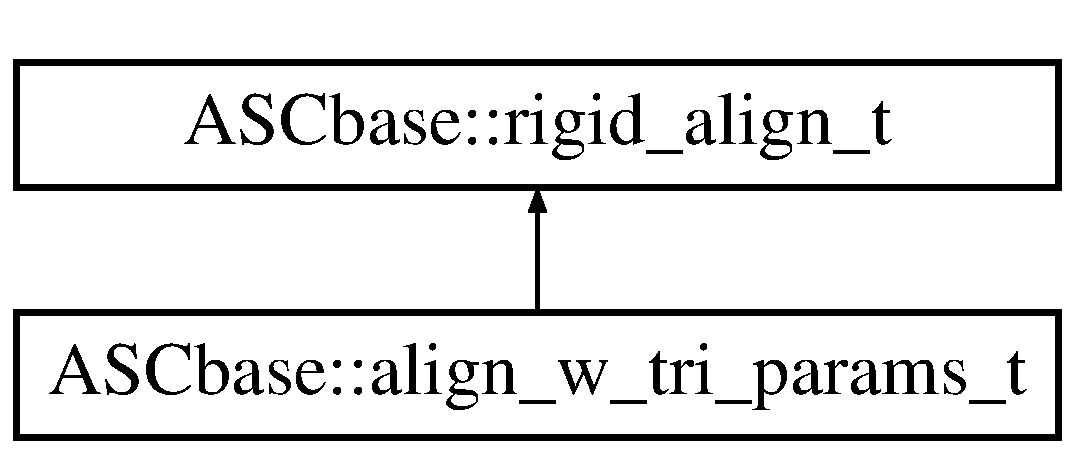
\includegraphics[height=2cm]{classASCbase_1_1align__w__tri__params__t}
\end{center}
\end{figure}
\subsection*{Public Member Functions}
\begin{CompactItemize}
\item 
\bf{align\_\-w\_\-tri\_\-params\_\-t} (const \bf{align\_\-w\_\-tri\_\-params\_\-t} \&other)\label{classASCbase_1_1align__w__tri__params__t_483a34c589f7b8c6ed5ccb0207436910}

\begin{CompactList}\small\item\em Basic copy constructor. \item\end{CompactList}\item 
const \bf{align\_\-w\_\-tri\_\-params\_\-t} \& \bf{operator=} (const \bf{align\_\-w\_\-tri\_\-params\_\-t} \&other)\label{classASCbase_1_1align__w__tri__params__t_db03dafc141cf94fc2b71250a00b8fdf}

\begin{CompactList}\small\item\em Basic assignment operator. \item\end{CompactList}\item 
virtual \bf{$\sim$align\_\-w\_\-tri\_\-params\_\-t} ()\label{classASCbase_1_1align__w__tri__params__t_09024ddae3c35629a39ffa0a20a50e66}

\begin{CompactList}\small\item\em Do nothing destructor. \item\end{CompactList}\item 
virtual void \textbf{write\_\-score\_\-fields} (std::ostream \&out, const uint orient\_\-num, const bool wrote\_\-ligs, const std::string \&ext\_\-SF\_\-id\_\-in, const std::string \&struct\_\-id, const std::string \&lig\_\-id) const \label{classASCbase_1_1align__w__tri__params__t_194cd244292abd6ce90cfc4f0164bcb1}

\item 
virtual void \textbf{write\_\-score\_\-fields} (std::ostream \&out) const \label{classASCbase_1_1align__w__tri__params__t_b7e7cb9ab0bf1e0a10801ec8667026cc}

\item 
virtual void \textbf{get\_\-score\_\-field\_\-labels} (std::vector$<$ std::string $>$ $\ast$fields, const bool normalize\_\-score) const \label{classASCbase_1_1align__w__tri__params__t_5f779560ad2881c71dc876a58df96763}

\item 
virtual void \textbf{set\_\-triangle\_\-params} (const my\_\-float\_\-t perimeter, const my\_\-float\_\-t long\_\-len, const my\_\-float\_\-t short\_\-len)\label{classASCbase_1_1align__w__tri__params__t_067127f641ca7407b5eb01900d0c8ec8}

\item 
virtual void \textbf{set\_\-number\_\-of\_\-orientations} (const size\_\-t num)\label{classASCbase_1_1align__w__tri__params__t_f9c57b30b02ee6202689c3a5083b47a6}

\end{CompactItemize}
\subsection*{Private Member Functions}
\begin{CompactItemize}
\item 
void \textbf{init} ()\label{classASCbase_1_1align__w__tri__params__t_21f99cdf72bd080020c80bb787238850}

\item 
void \textbf{do\_\-copy} (const \bf{align\_\-w\_\-tri\_\-params\_\-t} \&other)\label{classASCbase_1_1align__w__tri__params__t_d13773949adc8a04a545163e0c0bd70b}

\end{CompactItemize}
\subsection*{Private Attributes}
\begin{CompactItemize}
\item 
my\_\-float\_\-t \textbf{A\_\-perimeter}\label{classASCbase_1_1align__w__tri__params__t_809692e4cdff137a10bcc0a6d3435f22}

\item 
my\_\-float\_\-t \textbf{A\_\-long\_\-len}\label{classASCbase_1_1align__w__tri__params__t_d8d0c543b711b70da6acbdfa4b5d2250}

\item 
my\_\-float\_\-t \textbf{A\_\-short\_\-len}\label{classASCbase_1_1align__w__tri__params__t_1fd1f4c5f12a0e9f777dd1eab5addde2}

\item 
size\_\-t \textbf{A\_\-num\_\-orients}\label{classASCbase_1_1align__w__tri__params__t_b97ddf7a0ca9396114e63dc72d72dfe2}

\end{CompactItemize}


\subsection{Detailed Description}
addition of triangle parameters to saved alignments 



The documentation for this class was generated from the following file:\begin{CompactItemize}
\item 
new\_\-tri\_\-test.H\end{CompactItemize}

\section{ASCbase::Alignments\-From\-Results\-File Class Reference}
\label{classASCbase_1_1AlignmentsFromResultsFile}\index{ASCbase::AlignmentsFromResultsFile@{ASCbase::AlignmentsFromResultsFile}}
Class to score alignments in a given Sim\-Site3D results file.  


{\tt \#include $<$Alignments\-From\-Results\-File.H$>$}

\subsection*{Public Member Functions}
\begin{CompactItemize}
\item 
\bf{Alignments\-From\-Results\-File} (const std::string res\_\-fname)\label{classASCbase_1_1AlignmentsFromResultsFile_0834e02449a91cc81b01e44566b3ca9c}

\begin{CompactList}\small\item\em Cstor. \item\end{CompactList}\item 
virtual \bf{$\sim$Alignments\-From\-Results\-File} ()\label{classASCbase_1_1AlignmentsFromResultsFile_ac17079e981f15b11ff09284843f1c60}

\begin{CompactList}\small\item\em basic destruction \item\end{CompactList}\item 
template$<$typename align\_\-T$>$ bool \bf{align} (\bf{Model\-Sitemap} $\ast$query\_\-site, \bf{Sitemap} \&dset\_\-site, std::vector$<$ align\_\-T $>$ $\ast$alignments)\label{classASCbase_1_1AlignmentsFromResultsFile_8a607016b81b625aa0debaa1d469067d}

\begin{CompactList}\small\item\em Required alignment method. \item\end{CompactList}\end{CompactItemize}
\subsection*{Private Attributes}
\begin{CompactItemize}
\item 
std::string \textbf{A\_\-res\_\-fname}\label{classASCbase_1_1AlignmentsFromResultsFile_629d9546382d3f8879e8a324b392584e}

\end{CompactItemize}


\subsection{Detailed Description}
Class to score alignments in a given Sim\-Site3D results file. 

NOTE: this method is inefficient in that it will scan the entire results file each time it is called -- this is to avoid the problem of very long results files that cannot fit in memory. 



The documentation for this class was generated from the following file:\begin{CompactItemize}
\item 
Alignments\-From\-Results\-File.H\end{CompactItemize}

\section{ASCbase::All\-Pairs\-Sitemap\-Test Class Reference}
\label{classASCbase_1_1AllPairsSitemapTest}\index{ASCbase::AllPairsSitemapTest@{ASCbase::AllPairsSitemapTest}}
{\tt \#include $<$All\-Pairs\-Sitemap\-Test.H$>$}

Inheritance diagram for ASCbase::All\-Pairs\-Sitemap\-Test::\begin{figure}[H]
\begin{center}
\leavevmode
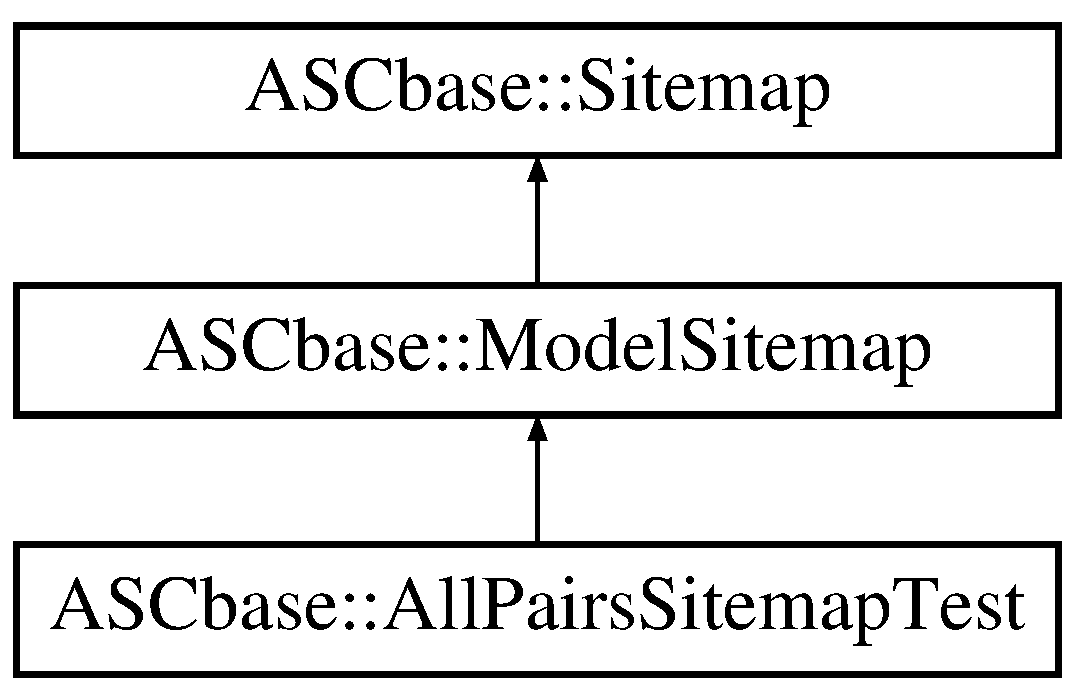
\includegraphics[height=3cm]{classASCbase_1_1AllPairsSitemapTest}
\end{center}
\end{figure}
\subsection*{Public Member Functions}
\begin{CompactItemize}
\item 
\textbf{All\-Pairs\-Sitemap\-Test} (const std::string path, const std::string struct\_\-id, const \bf{Base\-Parameters} \&args, const bool normalize=false, const bool load\_\-hbond\_\-surfaces=false, const bool hydrophobic\_\-query=false)\label{classASCbase_1_1AllPairsSitemapTest_52089682608f8e316aebbea656518f15}

\item 
bool \bf{get\_\-bucket\_\-iters} (const uint c, const my\_\-float\_\-t perimeter, const my\_\-float\_\-t max\_\-len, const my\_\-float\_\-t min\_\-len, bucket\_\-vci $\ast$bucket\_\-begin, bucket\_\-vci $\ast$bucket\_\-end)
\begin{CompactList}\small\item\em Given c,p,l,s get the iterators for the corresponding color bucket. \item\end{CompactList}\end{CompactItemize}
\subsection*{Private Member Functions}
\begin{CompactItemize}
\item 
void \textbf{create\_\-color\_\-bins} ()\label{classASCbase_1_1AllPairsSitemapTest_56096e393e198026ec9c90dc307114da}

\end{CompactItemize}
\subsection*{Private Attributes}
\begin{CompactItemize}
\item 
idx\_\-tbl\_\-lvl\_\-long \bf{A\_\-color\_\-bins}\label{classASCbase_1_1AllPairsSitemapTest_c51b3ea8452f20ddd328f0d87c45f931}

\begin{CompactList}\small\item\em Abuse the name ... \item\end{CompactList}\item 
std::list$<$ \bf{triangle\_\-t} $>$ \bf{A\_\-why\_\-use\_\-a\_\-list}\label{classASCbase_1_1AllPairsSitemapTest_9271d3343a1d725eaea89fbda620fd57}

\begin{CompactList}\small\item\em A double pass is likely to be more efficient -- first populate the vector, then hold it constant while determining the iterators for each bin. \item\end{CompactList}\end{CompactItemize}
\subsection*{Static Private Attributes}
\begin{CompactItemize}
\item 
static const std::string \bf{A\_\-fname}\label{classASCbase_1_1AllPairsSitemapTest_3e83862c6f07ad04b38d29404760b5dc}

\begin{CompactList}\small\item\em Source file name. \item\end{CompactList}\end{CompactItemize}


\subsection{Detailed Description}
This class is implemented in a kludge manner so that the interface for get\_\-bucket\_\-iters is the same as that for Model\-Sitemaps. We don't really care about speed penalty here as it is not production code 



\subsection{Member Function Documentation}
\index{ASCbase::AllPairsSitemapTest@{ASCbase::All\-Pairs\-Sitemap\-Test}!get_bucket_iters@{get\_\-bucket\_\-iters}}
\index{get_bucket_iters@{get\_\-bucket\_\-iters}!ASCbase::AllPairsSitemapTest@{ASCbase::All\-Pairs\-Sitemap\-Test}}
\subsubsection{\setlength{\rightskip}{0pt plus 5cm}bool ASCbase::All\-Pairs\-Sitemap\-Test::get\_\-bucket\_\-iters (const uint {\em c}, const my\_\-float\_\-t {\em perimeter}, const my\_\-float\_\-t {\em max\_\-len}, const my\_\-float\_\-t {\em min\_\-len}, bucket\_\-vci $\ast$ {\em bucket\_\-begin}, bucket\_\-vci $\ast$ {\em bucket\_\-end})\hspace{0.3cm}{\tt  [inline, virtual]}}\label{classASCbase_1_1AllPairsSitemapTest_662913221bdc0a3063def4d40dd0d6f5}


Given c,p,l,s get the iterators for the corresponding color bucket. 

Given a \char`\"{}color\char`\"{}, get all the triangles with that color via iterators to the begin and end of the bucket.

\begin{Desc}
\item[Parameters:]
\begin{description}
\item[{\em c}]hash\_\-class index \item[{\em p}]perimeter level index -- not used in this class \item[{\em l}]longest edge length index -- not used in this class \item[{\em s}]shortest edge length index -- not used in this class \item[{\em bucket\_\-begin}]Pointer to the beginning of the bucket \item[{\em bucket\_\-end}]Pointer to the end of the bucket \end{description}
\end{Desc}
\begin{Desc}
\item[Returns:]true if bucket is nonempty \end{Desc}


Reimplemented from \bf{ASCbase::Model\-Sitemap} \doxyref{p.}{classASCbase_1_1ModelSitemap_c80869d4e5b99f09d776f48c157fd52c}.

The documentation for this class was generated from the following file:\begin{CompactItemize}
\item 
All\-Pairs\-Sitemap\-Test.H\end{CompactItemize}

\section{ASCbase::geometry::arc\_\-t Class Reference}
\label{classASCbase_1_1geometry_1_1arc__t}\index{ASCbase::geometry::arc_t@{ASCbase::geometry::arc\_\-t}}
Computational analytic representation of a 3D arc.  


{\tt \#include $<$sphere.H$>$}

\subsection*{Public Member Functions}
\begin{CompactItemize}
\item 
\bf{arc\_\-t} (const sphere\_\-t \&S, const my\_\-float\_\-t $\ast$end\_\-pt0, const my\_\-float\_\-t $\ast$mid\_\-pt, const my\_\-float\_\-t $\ast$end\_\-pt1)\label{classASCbase_1_1geometry_1_1arc__t_fd9cea33957ae88b1f380bf809cbbff6}

\begin{CompactList}\small\item\em Initialize the arc by a sphere \& arc end points \& arc mid point. \item\end{CompactList}\item 
\bf{arc\_\-t} (const \bf{arc\_\-t} \&src)\label{classASCbase_1_1geometry_1_1arc__t_18b1410a465b4add59d54d8654bf8842}

\begin{CompactList}\small\item\em Copy constructor. \item\end{CompactList}\item 
const \bf{arc\_\-t} \& \textbf{operator=} (const \bf{arc\_\-t} \&src)\label{classASCbase_1_1geometry_1_1arc__t_3b16dc08c008f6d80be326665a19a1a1}

\item 
const bool \bf{contains} (const my\_\-float\_\-t $\ast$pt) const \label{classASCbase_1_1geometry_1_1arc__t_01ba159b58239264350e90caa746dca7}

\begin{CompactList}\small\item\em Is point contained in arc? \item\end{CompactList}\item 
void \bf{intersection} (const \bf{arc\_\-t} \&other, std::vector$<$ \bf{arc\_\-t} $>$ $\ast$I\_\-arcs)
\item 
const bool \textbf{operator==} (const \bf{arc\_\-t} \&other)\label{classASCbase_1_1geometry_1_1arc__t_b08aec83d224c06d7b35f6fdcc70d478}

\item 
const my\_\-float\_\-t $\ast$ \textbf{end\_\-pts} () const \label{classASCbase_1_1geometry_1_1arc__t_1aa54d4a368b5f54286d5b1a2694da6e}

\item 
const my\_\-float\_\-t $\ast$ \bf{get\_\-mid\_\-pt} () const 
\item 
const my\_\-float\_\-t $\ast$ \textbf{in\_\-dir} () const \label{classASCbase_1_1geometry_1_1arc__t_6d0b6a1eaa18fda15db3053be0a6c6f6}

\end{CompactItemize}
\subsection*{Private Member Functions}
\begin{CompactItemize}
\item 
void \bf{arc\_\-mid\_\-point} (const my\_\-float\_\-t $\ast$end\_\-pt0, const my\_\-float\_\-t $\ast$end\_\-pt1, my\_\-float\_\-t $\ast$mid\_\-pt, my\_\-float\_\-t $\ast$mid\_\-pt\_\-dir)\label{classASCbase_1_1geometry_1_1arc__t_bf87d7083d0b036b8aa49a8f76091462}

\begin{CompactList}\small\item\em Compute the mid point of an arc. \item\end{CompactList}\item 
void \textbf{compute\_\-overlap} (const my\_\-float\_\-t $\ast$self\_\-end\_\-pt, const my\_\-float\_\-t $\ast$other\_\-end\_\-pt, std::vector$<$ \bf{arc\_\-t} $>$ $\ast$I\_\-arcs, my\_\-float\_\-t $\ast$my\_\-dir)\label{classASCbase_1_1geometry_1_1arc__t_ec22f353635ed13d58a1f0eacd704ffd}

\item 
void \textbf{do\_\-copy} (const \bf{arc\_\-t} \&src)\label{classASCbase_1_1geometry_1_1arc__t_c999379b32c2d80997fd5cdb3503693f}

\end{CompactItemize}
\subsection*{Private Attributes}
\begin{CompactItemize}
\item 
sphere\_\-t \bf{A\_\-S}\label{classASCbase_1_1geometry_1_1arc__t_61808b252a9a77e07388ef89cb717781}

\begin{CompactList}\small\item\em Sphere on which the arc lies. \item\end{CompactList}\item 
my\_\-float\_\-t \bf{A\_\-end\_\-pts} [6]\label{classASCbase_1_1geometry_1_1arc__t_23ed7beb59a38ee8e970536506e46429}

\begin{CompactList}\small\item\em End points of the arc. \item\end{CompactList}\item 
my\_\-float\_\-t \bf{A\_\-mid\_\-pt} [3]\label{classASCbase_1_1geometry_1_1arc__t_abb892372174ae16d4485cd46ceb5aac}

\begin{CompactList}\small\item\em Mid point of the arc. \item\end{CompactList}\item 
my\_\-float\_\-t \bf{A\_\-in\_\-dir} [3]\label{classASCbase_1_1geometry_1_1arc__t_a945c545c3b2ac14757f8cc6bf9326df}

\begin{CompactList}\small\item\em vector; S.center -$>$ mid\_\-pt \item\end{CompactList}\item 
my\_\-float\_\-t \bf{A\_\-chord\_\-mid\_\-pt} [3]\label{classASCbase_1_1geometry_1_1arc__t_e5da612f0b29559898b76854005028f7}

\begin{CompactList}\small\item\em Mid point of chord defined by end\_\-pts. \item\end{CompactList}\end{CompactItemize}
\subsection*{Friends}
\begin{CompactItemize}
\item 
std::ostream \& \textbf{operator$<$$<$} (std::ostream \&out, const \bf{arc\_\-t} \&A)\label{classASCbase_1_1geometry_1_1arc__t_448902453ee3eb5a63e4bcfd54c2c5b8}

\end{CompactItemize}


\subsection{Detailed Description}
Computational analytic representation of a 3D arc. 



\subsection{Member Function Documentation}
\index{ASCbase::geometry::arc_t@{ASCbase::geometry::arc\_\-t}!get_mid_pt@{get\_\-mid\_\-pt}}
\index{get_mid_pt@{get\_\-mid\_\-pt}!ASCbase::geometry::arc_t@{ASCbase::geometry::arc\_\-t}}
\subsubsection{\setlength{\rightskip}{0pt plus 5cm}const my\_\-float\_\-t$\ast$ ASCbase::geometry::arc\_\-t::get\_\-mid\_\-pt () const\hspace{0.3cm}{\tt  [inline]}}\label{classASCbase_1_1geometry_1_1arc__t_86f92d310b8cc785ae09c45201f97258}


named get\_\-mid\_\-pt since I am too lazy to change all the local variables with the name mid\_\-pt \index{ASCbase::geometry::arc_t@{ASCbase::geometry::arc\_\-t}!intersection@{intersection}}
\index{intersection@{intersection}!ASCbase::geometry::arc_t@{ASCbase::geometry::arc\_\-t}}
\subsubsection{\setlength{\rightskip}{0pt plus 5cm}void ASCbase::geometry::arc\_\-t::intersection (const \bf{arc\_\-t} \& {\em other}, std::vector$<$ \bf{arc\_\-t} $>$ $\ast$ {\em I\_\-arcs})\hspace{0.3cm}{\tt  [inline]}}\label{classASCbase_1_1geometry_1_1arc__t_05ed53967368242ccad327e056f1d897}


Assumption: Both arcs lie on the same circle 

The documentation for this class was generated from the following file:\begin{CompactItemize}
\item 
sphere.H\end{CompactItemize}

\section{ASCbase::atom\_\-conv\_\-type Struct Reference}
\label{structASCbase_1_1atom__conv__type}\index{ASCbase::atom_conv_type@{ASCbase::atom\_\-conv\_\-type}}
Silly little struct to help convert from string to atom\_\-type.  


{\tt \#include $<$Atom\-Types.H$>$}

\subsection*{Public Attributes}
\begin{CompactItemize}
\item 
atom\_\-type \textbf{atom}\label{structASCbase_1_1atom__conv__type_a815b2f900fc36004e1cfa6abae799e2}

\item 
std::string \textbf{name}\label{structASCbase_1_1atom__conv__type_92e7ee024a311135ac0e9121d6b50eab}

\end{CompactItemize}


\subsection{Detailed Description}
Silly little struct to help convert from string to atom\_\-type. 



The documentation for this struct was generated from the following file:\begin{CompactItemize}
\item 
Atom\-Types.H\end{CompactItemize}

\section{ASCbase::atom\_\-info\_\-t Struct Reference}
\label{structASCbase_1_1atom__info__t}\index{ASCbase::atom_info_t@{ASCbase::atom\_\-info\_\-t}}
{\tt \#include $<$Atom\-Types.H$>$}

\subsection*{Public Attributes}
\begin{CompactItemize}
\item 
atom\_\-type \bf{atom}\label{structASCbase_1_1atom__info__t_3a8ad1a87e0f8c0e9e20c6b7a3b53e51}

\begin{CompactList}\small\item\em ASCbase atom identifier (enum). \item\end{CompactList}\item 
orbit\_\-type \bf{orbit}\label{structASCbase_1_1atom__info__t_fcebe437b571a4ac9ff7b4dfa319b1d7}

\begin{CompactList}\small\item\em ASCbase atom orbital identifier (enum). \item\end{CompactList}\item 
my\_\-float\_\-t \bf{vdw\_\-radius}\label{structASCbase_1_1atom__info__t_1d6e93f1fc9c78af5bec80786d7560f6}

\begin{CompactList}\small\item\em Van der Waals radius. \item\end{CompactList}\end{CompactItemize}


\subsection{Detailed Description}
The Van der Waals radii of a number of metals are the recommended values given in table 12 of S. S. Batsanov, \char`\"{}Van der Waals radii of elements from the data of structural inorganic chemistry\char`\"{}, Russian Chemical Bulletin, V. 44, 1995. 



The documentation for this struct was generated from the following file:\begin{CompactItemize}
\item 
Atom\-Types.H\end{CompactItemize}

\section{ASCbase::atom\_\-t Class Reference}
\label{classASCbase_1_1atom__t}\index{ASCbase::atom_t@{ASCbase::atom\_\-t}}
Generic atom type which uses the \doxyref{point\_\-t}{p.}{classASCbase_1_1point__t} class to store its position.  


{\tt \#include $<$atom.H$>$}

Inheritance diagram for ASCbase::atom\_\-t::\begin{figure}[H]
\begin{center}
\leavevmode
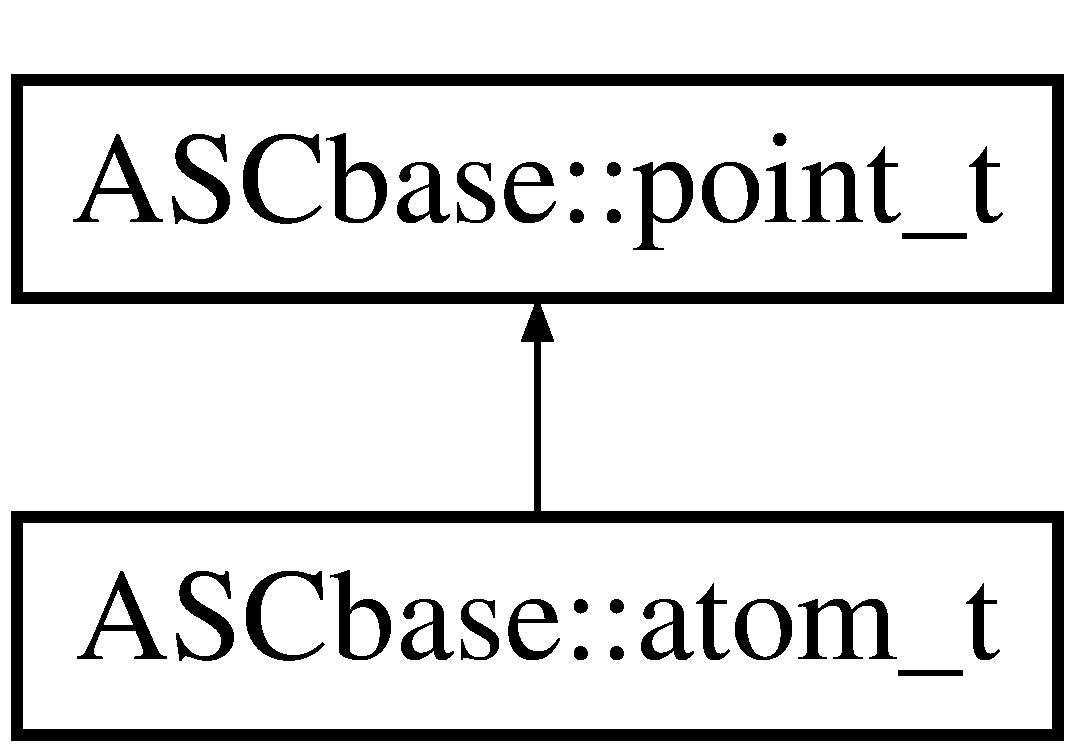
\includegraphics[height=2cm]{classASCbase_1_1atom__t}
\end{center}
\end{figure}
\subsection*{Public Member Functions}
\begin{CompactItemize}
\item 
\textbf{atom\_\-t} (alloc\_\-t a=ALLOC\_\-POSITION)\label{classASCbase_1_1atom__t_ba80852410e7bad5e93cae7e65e00d4b}

\item 
\textbf{atom\_\-t} (const \bf{atom\_\-t} \&a)\label{classASCbase_1_1atom__t_a27845e51201a1929c21ebcf7fa92a89}

\item 
const \bf{atom\_\-t} \& \textbf{operator=} (const \bf{atom\_\-t} \&a)\label{classASCbase_1_1atom__t_aebc062942c27c6a4ecc451e95e0ca51}

\item 
const bool \bf{is\_\-water} () const \label{classASCbase_1_1atom__t_77399ac0cfa6b5d267e92b9d476a2465}

\begin{CompactList}\small\item\em Allows flexibility in how waters are designated. \item\end{CompactList}\item 
const bool \bf{is\_\-metal} () const \label{classASCbase_1_1atom__t_4e560e164d125669d08aa9525d34216e}

\begin{CompactList}\small\item\em Allows flexibility in how metals are designated. \item\end{CompactList}\item 
const bool \textbf{is\_\-nitrogen} () const \label{classASCbase_1_1atom__t_bee03028777568b3e13d6c757d0cfd17}

\item 
const bool \textbf{is\_\-oxygen} () const \label{classASCbase_1_1atom__t_0c4ce066143157a201c9504bb0778d0f}

\item 
const bool \textbf{is\_\-hydrophobic} () const \label{classASCbase_1_1atom__t_c151b67632a833125bc4edd7eeaa079c}

\item 
const bool \textbf{is\_\-hbonder} () const \label{classASCbase_1_1atom__t_b5818f32a48da4ef0da634e9c5d52ccb}

\end{CompactItemize}
\subsection*{Static Public Member Functions}
\begin{CompactItemize}
\item 
static bool \bf{cmp} (const \bf{atom\_\-t} \&A, const \bf{atom\_\-t} \&B)\label{classASCbase_1_1atom__t_0e4ddf2772215a45e107615b3a144537}

\begin{CompactList}\small\item\em Allows sorting of an atom\_\-vec\_\-t by atom number. \item\end{CompactList}\end{CompactItemize}
\subsection*{Public Attributes}
\begin{CompactItemize}
\item 
uint \bf{atom\_\-num}\label{classASCbase_1_1atom__t_9a854374ed82fbc5e7f29690cd7f2418}

\begin{CompactList}\small\item\em Atom (serial) number. \item\end{CompactList}\item 
uint \bf{res\_\-num}\label{classASCbase_1_1atom__t_4a643f052098c53dd7cfe1e6f17462a0}

\begin{CompactList}\small\item\em Residue number. \item\end{CompactList}\item 
atom\_\-type \bf{name}\label{classASCbase_1_1atom__t_8d17fc5f8e49ef5e1bea2e89a0b6e600}

\begin{CompactList}\small\item\em Atom type. \item\end{CompactList}\item 
residue\_\-type \bf{res}\label{classASCbase_1_1atom__t_b3b7b5f7e8172387dd581dcacc4a9f72}

\begin{CompactList}\small\item\em Residue type. \item\end{CompactList}\item 
char \bf{chain\-ID}\label{classASCbase_1_1atom__t_b4a4060dde7bf73e494332146ed5ca92}

\begin{CompactList}\small\item\em Chain id. \item\end{CompactList}\item 
char \bf{alt\-Loc}\label{classASCbase_1_1atom__t_7e7d73ecb81a7923c92284e4c86bfc5c}

\begin{CompactList}\small\item\em Alterate location code. \item\end{CompactList}\item 
char \bf{i\-Code}\label{classASCbase_1_1atom__t_f7a846d9ffb1b0caf8a7b7b88bcf2f32}

\begin{CompactList}\small\item\em Insertion code. \item\end{CompactList}\item 
my\_\-float\_\-t \bf{occupancy}\label{classASCbase_1_1atom__t_e9d0dc62c74dc8e3cf8c4a8d9866170a}

\begin{CompactList}\small\item\em Occupancy value. \item\end{CompactList}\item 
my\_\-float\_\-t \bf{temp\-Factor}\label{classASCbase_1_1atom__t_6a08edf1e9a8fc861d434a81e306da39}

\begin{CompactList}\small\item\em Temperature factor. \item\end{CompactList}\item 
orbit\_\-type \bf{orbit}\label{classASCbase_1_1atom__t_0a438d9b577cedf15ac1629c3067e2a7}

\begin{CompactList}\small\item\em Atom hybridization/orbital. \item\end{CompactList}\item 
my\_\-float\_\-t \bf{vdw\_\-radius}\label{classASCbase_1_1atom__t_1beb46018c79fd73df622a22540c341a}

\begin{CompactList}\small\item\em Atom's Van der Waals radius. \item\end{CompactList}\item 
std::string \bf{name\_\-str}\label{classASCbase_1_1atom__t_bb5f12af2e89540a14e1d2ed78905a97}

\begin{CompactList}\small\item\em For PDB HETATMs', PDB Hs' and mol2 atoms' names. \item\end{CompactList}\item 
std::string \bf{res\_\-str}\label{classASCbase_1_1atom__t_16c11a15f4136c3d4bb29e9abd6fa719}

\begin{CompactList}\small\item\em For PDB HETATMs. \item\end{CompactList}\item 
bool \bf{is\_\-hetero}\label{classASCbase_1_1atom__t_d4583a7bfb72db12ae7eccbb2c232714}

\begin{CompactList}\small\item\em True implies PDB HETATM, otherwise false. \item\end{CompactList}\item 
interaction\-Type \bf{act\_\-type}\label{classASCbase_1_1atom__t_0649f5881857d9437b85dfec852f5a88}

\begin{CompactList}\small\item\em Donor, acceptor, doneptor, hphob, or nothing. \item\end{CompactList}\item 
my\_\-float\_\-t \bf{charge}\label{classASCbase_1_1atom__t_5b15b577b1e6874f1ca87a3a972ba212}

\begin{CompactList}\small\item\em Protein charges + ASCbase summed atomic charges on ligands. \item\end{CompactList}\item 
my\_\-float\_\-t \bf{orig\_\-charge}\label{classASCbase_1_1atom__t_1bdb3b1e702e49621bcbcfcee908e9c6}

\begin{CompactList}\small\item\em Hold the ligand atomic charges as read in. \item\end{CompactList}\item 
int \bf{subst\_\-id}\label{classASCbase_1_1atom__t_6e71b7884ac0a9e5526ce40f2a807cf9}

\begin{CompactList}\small\item\em mol2 junk -- ignored for now \item\end{CompactList}\item 
std::string \bf{subst\_\-name}\label{classASCbase_1_1atom__t_41715c0d9c29a54ee6b8b1fe979c49b6}

\begin{CompactList}\small\item\em mol2 junk -- ignored for now \item\end{CompactList}\item 
int \bf{hydro}\label{classASCbase_1_1atom__t_f1eaec85b84f948e97692a58dbfa2526}

\begin{CompactList}\small\item\em Hydrophobicity value. \item\end{CompactList}\end{CompactItemize}
\subsection*{Static Public Attributes}
\begin{CompactItemize}
\item 
static const \bf{atom\_\-t} \bf{NULL\_\-ATOM}\label{classASCbase_1_1atom__t_3bdee8ba5c2e5b44c68458d9640f1051}

\begin{CompactList}\small\item\em the \char`\"{}standard\char`\"{} null atom \item\end{CompactList}\item 
static const \bf{point\_\-storage}$<$ \bf{atom\_\-t} $>$ \bf{NULL\_\-ATOM\_\-VECTOR}\label{classASCbase_1_1atom__t_7d84cd97fa838e1ab2452a1794e723bc}

\begin{CompactList}\small\item\em the \char`\"{}standard\char`\"{} null atom vector \item\end{CompactList}\item 
static const \bf{point\_\-storage}$<$ \bf{atom\_\-t} $>$::const\_\-iterator \bf{NULL\_\-ATOM\_\-VCI} = atom\_\-t::NULL\_\-ATOM\_\-VECTOR.begin()\label{classASCbase_1_1atom__t_6006207a0eed1857af230dca1dadc4a1}

\begin{CompactList}\small\item\em the \char`\"{}standard\char`\"{} null atom vector constant iterator \item\end{CompactList}\end{CompactItemize}
\subsection*{Private Member Functions}
\begin{CompactItemize}
\item 
void \textbf{do\_\-copy} (const \bf{atom\_\-t} \&a)\label{classASCbase_1_1atom__t_e3e92a459d6ad8b6a37fd2a3d7197324}

\end{CompactItemize}
\subsection*{Friends}
\begin{CompactItemize}
\item 
std::ostream \& \textbf{operator$<$$<$} (std::ostream \&out, const \bf{atom\_\-t} \&a)\label{classASCbase_1_1atom__t_d16a721f1511a95a28b046847e2d137e}

\end{CompactItemize}


\subsection{Detailed Description}
Generic atom type which uses the \doxyref{point\_\-t}{p.}{classASCbase_1_1point__t} class to store its position. 



The documentation for this class was generated from the following files:\begin{CompactItemize}
\item 
atom.H\item 
atom.C\end{CompactItemize}

\section{ASCbase::Atom\-Types Class Reference}
\label{classASCbase_1_1AtomTypes}\index{ASCbase::AtomTypes@{ASCbase::AtomTypes}}
{\tt \#include $<$Atom\-Types.H$>$}

\subsection*{Static Public Member Functions}
\begin{CompactItemize}
\item 
static const \bf{atom\_\-info\_\-t} $\ast$ \bf{lookup\_\-vdw\_\-rad} (const atom\_\-type atom, const orbit\_\-type orbit=DEFAULT\_\-ORBIT)
\end{CompactItemize}
\subsection*{Static Private Member Functions}
\begin{CompactItemize}
\item 
static void \bf{build\_\-vdw\_\-table} ()\label{classASCbase_1_1AtomTypes_e95076f4bd69e270be8e165cc069d153}

\begin{CompactList}\small\item\em Setup the map used to search for the atom's structure. \item\end{CompactList}\end{CompactItemize}
\subsection*{Static Private Attributes}
\begin{CompactItemize}
\item 
static std::multimap$<$ atom\_\-type, const \bf{atom\_\-info\_\-t} $\ast$ $>$ \textbf{vdw\_\-table}\label{classASCbase_1_1AtomTypes_a102e90d09161af7ffc880216dca0ad3}

\item 
static const uint \textbf{A\_\-atoms\_\-array\_\-size} = 81\label{classASCbase_1_1AtomTypes_ed91da828cc5373ae9b27f319fde0cdb}

\item 
static const \bf{atom\_\-info\_\-t} \textbf{A\_\-atoms\_\-array} [$\,$]\label{classASCbase_1_1AtomTypes_e776363cc2e100e676fefb550fbda1e6}

\end{CompactItemize}


\subsection{Detailed Description}
A data class to look up the \char`\"{}hard coded\char`\"{} data for a particular atom based on its name and orbital. 



\subsection{Member Function Documentation}
\index{ASCbase::AtomTypes@{ASCbase::Atom\-Types}!lookup_vdw_rad@{lookup\_\-vdw\_\-rad}}
\index{lookup_vdw_rad@{lookup\_\-vdw\_\-rad}!ASCbase::AtomTypes@{ASCbase::Atom\-Types}}
\subsubsection{\setlength{\rightskip}{0pt plus 5cm}static const \bf{atom\_\-info\_\-t}$\ast$ ASCbase::Atom\-Types::lookup\_\-vdw\_\-rad (const atom\_\-type {\em atom}, const orbit\_\-type {\em orbit} = {\tt DEFAULT\_\-ORBIT})\hspace{0.3cm}{\tt  [inline, static]}}\label{classASCbase_1_1AtomTypes_79594ad220d1951219aebe927c06626c}


\begin{Desc}
\item[Parameters:]
\begin{description}
\item[{\em atom}]Name type of the atom \item[{\em orbit}]Orbital type of the atom \end{description}
\end{Desc}
\begin{Desc}
\item[Returns:]constant pointer to the atom's \doxyref{atom\_\-info\_\-t}{p.}{structASCbase_1_1atom__info__t} \end{Desc}


The documentation for this class was generated from the following files:\begin{CompactItemize}
\item 
Atom\-Types.H\item 
Atom\-Types.C\end{CompactItemize}

\section{ASCbase::Ball Class Reference}
\label{classASCbase_1_1Ball}\index{ASCbase::Ball@{ASCbase::Ball}}
A spherical solid bounding volume.  


{\tt \#include $<$Bounding\-Volume.H$>$}

Inheritance diagram for ASCbase::Ball::\begin{figure}[H]
\begin{center}
\leavevmode
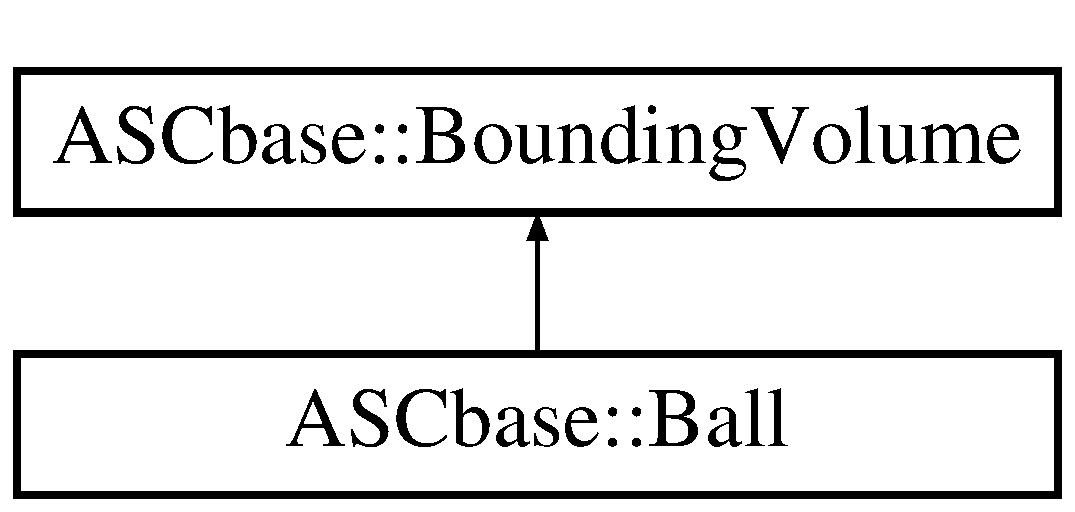
\includegraphics[height=2cm]{classASCbase_1_1Ball}
\end{center}
\end{figure}
\subsection*{Public Member Functions}
\begin{CompactItemize}
\item 
\textbf{Ball} (const my\_\-float\_\-t $\ast$center\_\-in, const my\_\-float\_\-t radius\_\-in, const my\_\-float\_\-t grid\_\-spacing=0.0)\label{classASCbase_1_1Ball_97e67bc08a56c79e9e959a632009ade6}

\item 
\textbf{Ball} (const \bf{Ball} \&src)\label{classASCbase_1_1Ball_75d5e1bf95a7262c6bc624dd12dfcc64}

\item 
virtual bool \bf{contains} (const my\_\-float\_\-t $\ast$point) const \label{classASCbase_1_1Ball_2f35f02b622dd5ab6a0587fea4decab9}

\begin{CompactList}\small\item\em Is the given point inside the bounding volume? \item\end{CompactList}\item 
virtual bool \textbf{BIND\_\-vol\_\-contains} (const my\_\-float\_\-t $\ast$point) const \label{classASCbase_1_1Ball_813573b67261525d0e929c403ada4edd}

\item 
virtual bool \textbf{RAD\_\-vol\_\-contains} (const my\_\-float\_\-t $\ast$point) const \label{classASCbase_1_1Ball_35f5cc5ed18329e95f9b76ec9e57341d}

\item 
virtual size\_\-t \bf{discretize} (const my\_\-float\_\-t spacing, my\_\-float\_\-t $\ast$$\ast$grid\_\-pts)\label{classASCbase_1_1Ball_a9f72b0b6f081f0d84907ae3dce7381b}

\begin{CompactList}\small\item\em discretize the volume using the spacing for grid spacing. \item\end{CompactList}\item 
virtual std::string \textbf{xml\_\-str} ()\label{classASCbase_1_1Ball_25e523c23461317176d63b322d700deb}

\end{CompactItemize}
\subsection*{Private Attributes}
\begin{CompactItemize}
\item 
my\_\-float\_\-t \textbf{center} [3]\label{classASCbase_1_1Ball_8cdfc3ec26ff94910d7a217fdf00b122}

\item 
my\_\-float\_\-t \textbf{radius}\label{classASCbase_1_1Ball_b10e3e683d98de2a313d95db8b1c2b5c}

\item 
my\_\-float\_\-t \textbf{rad\_\-squared}\label{classASCbase_1_1Ball_005b5e685fffb4e47e10ffba05f2c608}

\item 
my\_\-float\_\-t \textbf{BIND\_\-rad\_\-squared}\label{classASCbase_1_1Ball_46f12f5f5ce2f6ec63af22bb30cbcc39}

\item 
my\_\-float\_\-t \textbf{RAD\_\-rad\_\-squared}\label{classASCbase_1_1Ball_6124ef4765e6a8fb6653fae9fb06c927}

\end{CompactItemize}


\subsection{Detailed Description}
A spherical solid bounding volume. 



The documentation for this class was generated from the following files:\begin{CompactItemize}
\item 
Bounding\-Volume.H\item 
Bounding\-Volume.C\end{CompactItemize}

\section{ASCbase::Base\-Parameters Class Reference}
\label{classASCbase_1_1BaseParameters}\index{ASCbase::BaseParameters@{ASCbase::BaseParameters}}
{\tt \#include $<$Base\-Parameters.H$>$}

Inheritance diagram for ASCbase::Base\-Parameters::\begin{figure}[H]
\begin{center}
\leavevmode
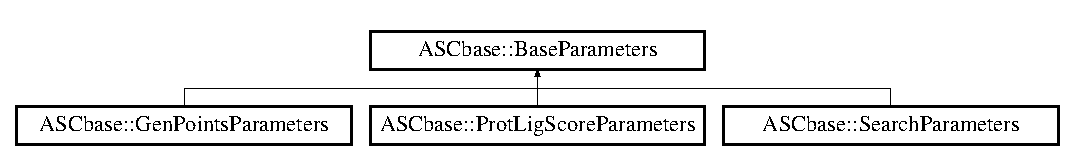
\includegraphics[height=1.72043cm]{classASCbase_1_1BaseParameters}
\end{center}
\end{figure}
\subsection*{Public Types}
\begin{CompactItemize}
\item 
\textbf{FATAL\_\-ERROR}\label{classASCbase_1_1BaseParameters_c80c7d6d1460ac21aee9af9e4adb27962ecf94b471dd1d92cfef939f1d8e5c5b}

\item 
\textbf{INVALID\_\-PARAMETER}\label{classASCbase_1_1BaseParameters_c80c7d6d1460ac21aee9af9e4adb27966a7dcbce394da1874589a864461ca96c}

\item 
\textbf{INITIALIZING}\label{classASCbase_1_1BaseParameters_c80c7d6d1460ac21aee9af9e4adb2796e0f14c6cff9f988fb50cd648984af4c8}

\item 
\textbf{DISPLAY\_\-HELP\_\-ONLY}\label{classASCbase_1_1BaseParameters_c80c7d6d1460ac21aee9af9e4adb2796009c052e63810d9249f5ba6d26733fcb}

\item 
\textbf{READY}\label{classASCbase_1_1BaseParameters_c80c7d6d1460ac21aee9af9e4adb27965688a5856aa9d26946abec13ed716dac}

\item 
enum \textbf{status\_\-t} \{ \par
\textbf{FATAL\_\-ERROR}, 
\textbf{INVALID\_\-PARAMETER}, 
\textbf{INITIALIZING}, 
\textbf{DISPLAY\_\-HELP\_\-ONLY}, 
\par
\textbf{READY}
 \}
\end{CompactItemize}
\subsection*{Public Member Functions}
\begin{CompactItemize}
\item 
status\_\-t \textbf{status} () const \label{classASCbase_1_1BaseParameters_39657de7d43af517724736e1c625546f}

\end{CompactItemize}
\subsection*{Static Public Member Functions}
\begin{CompactItemize}
\item 
static bool \textbf{get\_\-env\_\-var} (const std::string var, std::string $\ast$val)\label{classASCbase_1_1BaseParameters_f0c9884a0104f3b2e8595d401db60653}

\end{CompactItemize}
\subsection*{Public Attributes}
\begin{CompactItemize}
\item 
std::string \bf{dbase\_\-sites}\label{classASCbase_1_1BaseParameters_4812fa282e2ba266dbfa064182b594b9}

\begin{CompactList}\small\item\em Directory holding the database sitemaps. \item\end{CompactList}\item 
std::string \bf{dbase\_\-ligs}\label{classASCbase_1_1BaseParameters_d6b47ad4d8d7460817551da93171de4a}

\begin{CompactList}\small\item\em Directory holding the database ligands. \item\end{CompactList}\item 
std::string \bf{dbase\_\-prots}\label{classASCbase_1_1BaseParameters_fbb9b1185a994a991c0e68c30fa637b6}

\begin{CompactList}\small\item\em Directory holding the database proteins. \item\end{CompactList}\item 
std::string \bf{diverse\_\-sites}\label{classASCbase_1_1BaseParameters_89d38ef4448211e8ae3a63988e62f158}

\begin{CompactList}\small\item\em Directory holding the diverse sitemaps. \item\end{CompactList}\item 
std::string \bf{diverse\_\-ligs}\label{classASCbase_1_1BaseParameters_7431a50f3120b7f9f74026ad2c10b1a2}

\begin{CompactList}\small\item\em Directory holding ligands for diverse sitemaps. \item\end{CompactList}\item 
std::string \bf{proj\_\-output}\label{classASCbase_1_1BaseParameters_96522745ba23c6aac7d9258d65aac545}

\begin{CompactList}\small\item\em Directory to store results. \item\end{CompactList}\item 
std::string \bf{scratch\_\-dir}\label{classASCbase_1_1BaseParameters_96aa06a7fff08e400ec92d0ada56b786}

\begin{CompactList}\small\item\em Directory where ASCbase can create temp files. \item\end{CompactList}\item 
std::string \textbf{install\_\-dir}\label{classASCbase_1_1BaseParameters_6fc273afb61ac03e5e733e704b9003d5}

\item 
bool \textbf{load\_\-surf\_\-files}\label{classASCbase_1_1BaseParameters_dd007d2ec07c2f19ed5eb847cede37e7}

\item 
bool \textbf{require\_\-min\_\-npts}\label{classASCbase_1_1BaseParameters_2cbb07424c917a0593f1d40ea08bec81}

\end{CompactItemize}
\subsection*{Protected Member Functions}
\begin{CompactItemize}
\item 
bool \textbf{load\_\-conf\_\-file} (std::string conf\_\-fname)\label{classASCbase_1_1BaseParameters_0bb99f45e58ded09c08f202dc662fb2c}

\item 
void \textbf{print\_\-version} (std::ostream \&out, std::string prog\_\-name)\label{classASCbase_1_1BaseParameters_dd81fff1ee86b790d0ee408cf3834116}

\end{CompactItemize}
\subsection*{Protected Attributes}
\begin{CompactItemize}
\item 
status\_\-t \bf{A\_\-status}\label{classASCbase_1_1BaseParameters_552075c2455c9ce279594f9d620de06a}

\begin{CompactList}\small\item\em Parameter status. \item\end{CompactList}\end{CompactItemize}
\subsection*{Private Member Functions}
\begin{CompactItemize}
\item 
void \textbf{load\_\-environment} ()\label{classASCbase_1_1BaseParameters_d14f824ff3778e6eeadc6f280e712fa8}

\item 
void \textbf{init\_\-str\_\-to\_\-var\_\-map} ()\label{classASCbase_1_1BaseParameters_2b6efe90e6fc04c12a708793b134c337}

\end{CompactItemize}
\subsection*{Private Attributes}
\begin{CompactItemize}
\item 
std::map$<$ std::string, std::string $\ast$ $>$ \textbf{A\_\-str\_\-to\_\-var}\label{classASCbase_1_1BaseParameters_d2d6dce8fdb7bc506d95de45aa545b07}

\end{CompactItemize}
\subsection*{Static Private Attributes}
\begin{CompactItemize}
\item 
static const std::string \bf{A\_\-fname} = \char`\"{}Base\-Parameters.C\char`\"{}\label{classASCbase_1_1BaseParameters_41d22522d6af1b42c1ae142bba6190ca}

\begin{CompactList}\small\item\em Name of source file. \item\end{CompactList}\end{CompactItemize}


\subsection{Detailed Description}
The order is to first read the \$ASCBASE\_\-INSTALL\_\-DIR environment variable. Second, parse \$ASCBASE\_\-INSTALL\_\-DIR/ASCbase\-Soft\-Params/ascbase\_\-software.conf for system wide default values. Thirdly, check for any updated parameters in the environment. Finally, if load\_\-conf\_\-file is called by a derived class, the parsed values override all previously stored values. 



The documentation for this class was generated from the following files:\begin{CompactItemize}
\item 
Base\-Parameters.H\item 
Base\-Parameters.C\end{CompactItemize}

\section{ASCbase::Bounding\-Volume Class Reference}
\label{classASCbase_1_1BoundingVolume}\index{ASCbase::BoundingVolume@{ASCbase::BoundingVolume}}
Simple base class to define a common interface to 3D bounding volumes.  


{\tt \#include $<$Bounding\-Volume.H$>$}

Inheritance diagram for ASCbase::Bounding\-Volume::\begin{figure}[H]
\begin{center}
\leavevmode
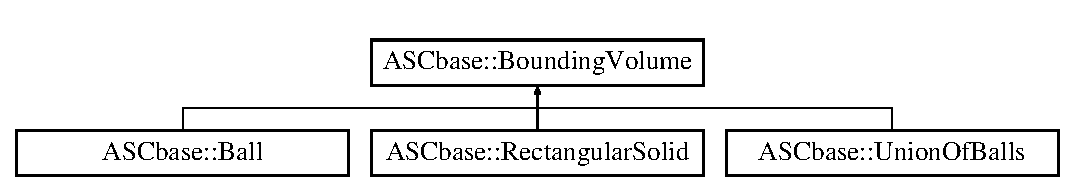
\includegraphics[height=2cm]{classASCbase_1_1BoundingVolume}
\end{center}
\end{figure}
\subsection*{Public Types}
\begin{CompactItemize}
\item 
\textbf{NULL\_\-VOLUME\_\-TYPE}\label{classASCbase_1_1BoundingVolume_90dd526306d995889c2ba0527d0e400c206c9d67d4ddcabdc42058538e90f223}

\item 
\textbf{RECTANGULAR\_\-SOLID}\label{classASCbase_1_1BoundingVolume_90dd526306d995889c2ba0527d0e400c978442c972efd3f68accee6a0a9f172c}

\item 
\textbf{SPHERE}\label{classASCbase_1_1BoundingVolume_90dd526306d995889c2ba0527d0e400cc10cb5a6a2c07cc74764081b2c34829d}

\item 
enum \textbf{volume\_\-t} \{ \textbf{NULL\_\-VOLUME\_\-TYPE}, 
\textbf{RECTANGULAR\_\-SOLID}, 
\textbf{SPHERE}
 \}
\end{CompactItemize}
\subsection*{Public Member Functions}
\begin{CompactItemize}
\item 
\bf{Bounding\-Volume} ()\label{classASCbase_1_1BoundingVolume_9fe70d0dcf235dd947304b1259e5dab3}

\begin{CompactList}\small\item\em Initialize pointers to NULL. \item\end{CompactList}\item 
\bf{Bounding\-Volume} (const \bf{Bounding\-Volume} \&src)\label{classASCbase_1_1BoundingVolume_460f07f7011383ee3bde18324fb216d8}

\begin{CompactList}\small\item\em Basic copy cstr. \item\end{CompactList}\item 
void \textbf{remove\_\-nonsurface\_\-points} (chain\_\-const\_\-iter \_\-begin, chain\_\-const\_\-iter \_\-end)\label{classASCbase_1_1BoundingVolume_7a552d8708eddcb0eb4b8af247eed3f3}

\item 
my\_\-float\_\-t \bf{dist\_\-to\_\-nearest\_\-grid\_\-pt} (const my\_\-float\_\-t $\ast$given\_\-pt, const my\_\-float\_\-t tol)\label{classASCbase_1_1BoundingVolume_29b827ac0631889832a23a6c3ccd73ad}

\begin{CompactList}\small\item\em Check if any grid point is within tolerance of given point. \item\end{CompactList}\item 
virtual bool \bf{contains} (const my\_\-float\_\-t $\ast$point) const =0\label{classASCbase_1_1BoundingVolume_4845f90aaeb0bdda5a7bab8ad69f249a}

\begin{CompactList}\small\item\em Is the given point inside the bounding volume? \item\end{CompactList}\item 
virtual bool \textbf{BIND\_\-vol\_\-contains} (const my\_\-float\_\-t $\ast$p) const =0\label{classASCbase_1_1BoundingVolume_fac13641d7742a874bdf8fc12bde2183}

\item 
virtual bool \textbf{RAD\_\-vol\_\-contains} (const my\_\-float\_\-t $\ast$p) const =0\label{classASCbase_1_1BoundingVolume_c7aa46af4a8298a435da9b8f04c6640f}

\item 
virtual size\_\-t \bf{discretize} (const my\_\-float\_\-t spacing, my\_\-float\_\-t $\ast$$\ast$grid\_\-pts)=0\label{classASCbase_1_1BoundingVolume_3e29c82e9883e18e948de572c28f778e}

\begin{CompactList}\small\item\em discretize the volume using the spacing for grid spacing. \item\end{CompactList}\item 
const my\_\-float\_\-t $\ast$ \textbf{grid\_\-points\_\-begin} () const \label{classASCbase_1_1BoundingVolume_6bbd9d6cfc903cc3684e9a8d4b6c4609}

\item 
const my\_\-float\_\-t $\ast$ \textbf{grid\_\-points\_\-end} () const \label{classASCbase_1_1BoundingVolume_bcd2ff2e80f5bdbd3838a589672caa92}

\item 
void \textbf{clear} ()\label{classASCbase_1_1BoundingVolume_238de4a44b0b1fd68bd3379f5abdb02c}

\item 
virtual std::string \textbf{xml\_\-str} ()=0\label{classASCbase_1_1BoundingVolume_edfa3d6c9da7269a8cc3b3361e1fce4b}

\end{CompactItemize}
\subsection*{Static Public Attributes}
\begin{CompactItemize}
\item 
static const my\_\-float\_\-t \textbf{MIN\_\-VDW\_\-DIST} = 2.5\label{classASCbase_1_1BoundingVolume_16eb8d31fe37eb14bf9b18f571cd32ad}

\end{CompactItemize}
\subsection*{Protected Member Functions}
\begin{CompactItemize}
\item 
void \textbf{copy\_\-points} (my\_\-float\_\-t $\ast$points, size\_\-t n, size\_\-t stride)\label{classASCbase_1_1BoundingVolume_276a47b97596ef8062112b0399e3c27c}

\item 
void \textbf{set\_\-grid\_\-points} (my\_\-float\_\-t $\ast$grid\_\-pts, const size\_\-t npts)\label{classASCbase_1_1BoundingVolume_9955a12346fe57b4a1a9bcc116a14c67}

\end{CompactItemize}
\subsection*{Static Protected Attributes}
\begin{CompactItemize}
\item 
static const my\_\-float\_\-t \textbf{MAXRADDIST} = 9.0\label{classASCbase_1_1BoundingVolume_a1cfa33783949f5c420c9887d6e51060}

\item 
static const my\_\-float\_\-t \textbf{MAXBINDDIST} = 5.0\label{classASCbase_1_1BoundingVolume_2309329304fbe3f248255dac05b91aa8}

\item 
static const std::string \bf{\_\-fname} = \char`\"{}Bounding\-Volume.C\char`\"{}\label{classASCbase_1_1BoundingVolume_ab8b9606c0e2f06271e6de0fbbae62af}

\begin{CompactList}\small\item\em source file name \item\end{CompactList}\end{CompactItemize}
\subsection*{Private Attributes}
\begin{CompactItemize}
\item 
my\_\-float\_\-t $\ast$ \textbf{grid\_\-pts\_\-beg}\label{classASCbase_1_1BoundingVolume_0c620a298e09563e4b8e63c4122a3864}

\item 
my\_\-float\_\-t $\ast$ \textbf{grid\_\-pts\_\-end}\label{classASCbase_1_1BoundingVolume_7cedadbeb63b343521502aacfed7f273}

\end{CompactItemize}
\subsection*{Static Private Attributes}
\begin{CompactItemize}
\item 
static const my\_\-float\_\-t \textbf{MAX\_\-HYDRO\_\-DIST} = 5.2\label{classASCbase_1_1BoundingVolume_bd0078867dd8810c162dc6c2cf096e6e}

\end{CompactItemize}


\subsection{Detailed Description}
Simple base class to define a common interface to 3D bounding volumes. 



The documentation for this class was generated from the following files:\begin{CompactItemize}
\item 
Bounding\-Volume.H\item 
Bounding\-Volume.C\end{CompactItemize}

\section{ASCbase::Coord\-File Class Reference}
\label{classASCbase_1_1CoordFile}\index{ASCbase::CoordFile@{ASCbase::CoordFile}}
{\tt \#include $<$Coord\-File.H$>$}

Inheritance diagram for ASCbase::Coord\-File::\begin{figure}[H]
\begin{center}
\leavevmode
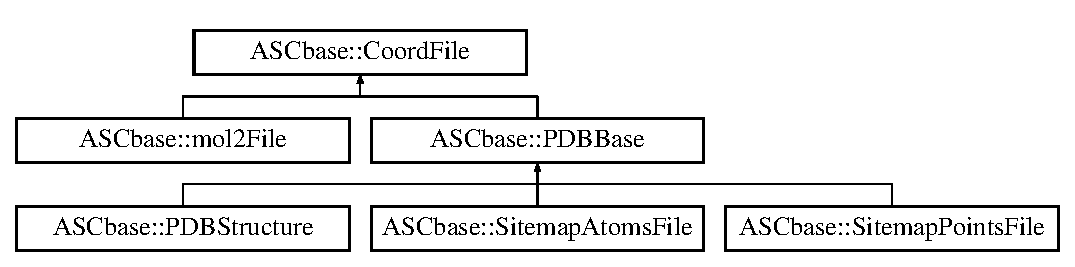
\includegraphics[height=3cm]{classASCbase_1_1CoordFile}
\end{center}
\end{figure}
\subsection*{Public Member Functions}
\begin{CompactItemize}
\item 
\bf{Coord\-File} ()\label{classASCbase_1_1CoordFile_7e9fbda616d8d9141663ded676268a4f}

\begin{CompactList}\small\item\em To be used when a file is to be created; initializes A\_\-fail to false. \item\end{CompactList}\item 
\bf{Coord\-File} (const std::string filename\_\-in, const verbose\_\-level\_\-t verbosity=VERBOSE\_\-SILENT)
\begin{CompactList}\small\item\em To be used when a file exists. \item\end{CompactList}\item 
\bf{Coord\-File} (const \bf{Coord\-File} \&src)
\item 
virtual \bf{$\sim$Coord\-File} ()\label{classASCbase_1_1CoordFile_b0646aae13c5714c541f9c0dfad334c7}

\begin{CompactList}\small\item\em Do nothing virtual dstr. \item\end{CompactList}\item 
virtual void \bf{report\_\-stats} (std::ostream \&out)=0
\begin{CompactList}\small\item\em Each derived class should support some routine to report on the file. \item\end{CompactList}\item 
virtual bool \bf{write} (const std::string filename)=0
\begin{CompactList}\small\item\em Each derived class should support some routine to write a molecule. \item\end{CompactList}\item 
atom\_\-vci \textbf{atoms\_\-begin} () const \label{classASCbase_1_1CoordFile_371501a34c2bb2315cda8cf5e3a8699d}

\item 
atom\_\-vci \textbf{atoms\_\-end} () const \label{classASCbase_1_1CoordFile_d17d0b45c944591dd5328eb65f59f044}

\item 
const my\_\-float\_\-t $\ast$ \textbf{positions\_\-begin} () const \label{classASCbase_1_1CoordFile_8f69771f77006ab8fe0f3bae830d9bbe}

\item 
const my\_\-float\_\-t $\ast$ \textbf{positions\_\-end} () const \label{classASCbase_1_1CoordFile_f7848c3d7d76d033bcbadf908a7eabc0}

\item 
atom\_\-vci \bf{get\_\-atom} (const uint atom\_\-num)\label{classASCbase_1_1CoordFile_c9649e85ff13ba1997fc8809401733d3}

\begin{CompactList}\small\item\em Assumes each atom in a coordinate file has a unique key (atom number). \item\end{CompactList}\item 
bool \bf{fail} () const \label{classASCbase_1_1CoordFile_62b4ac1cdf4bae7acb19ce63bfca599d}

\begin{CompactList}\small\item\em Check if any errors have occured when reading the atoms from file. \item\end{CompactList}\item 
std::string \bf{name} () const \label{classASCbase_1_1CoordFile_687a29cf9f287acaa3919c7cd11a1474}

\begin{CompactList}\small\item\em Get a string holding the name of the coordinate file. \item\end{CompactList}\item 
void \bf{transform} (const my\_\-float\_\-t $\ast$R, const my\_\-float\_\-t $\ast$T)\label{classASCbase_1_1CoordFile_e288ddf8441fe4652e6a1b90a4b5198c}

\begin{CompactList}\small\item\em Transform the positions. \item\end{CompactList}\item 
void \bf{inverse\_\-transform} (const my\_\-float\_\-t $\ast$R, const my\_\-float\_\-t $\ast$T)\label{classASCbase_1_1CoordFile_379c544ae1cd926491619e0f46532e27}

\begin{CompactList}\small\item\em Transform the positions by the inverse transformation. \item\end{CompactList}\item 
void \bf{revert} ()\label{classASCbase_1_1CoordFile_6f632e32959f743ccc307a16e04c1a96}

\begin{CompactList}\small\item\em Revert the current positions to the original positions. \item\end{CompactList}\item 
void \textbf{bin\_\-coordinates} (const my\_\-float\_\-t max\_\-dist)\label{classASCbase_1_1CoordFile_1ab04a131afbbd2cc4d59d2a2eb7ebb4}

\item 
atom\_\-vci \bf{closest\_\-atom} (const my\_\-float\_\-t $\ast$pos, my\_\-float\_\-t $\ast$d) const \label{classASCbase_1_1CoordFile_7727bbdac08565a2a01edad154108a49}

\begin{CompactList}\small\item\em Get the closest atom center to the given position. \item\end{CompactList}\item 
void \bf{close\_\-atoms} (const my\_\-float\_\-t $\ast$pos, const my\_\-float\_\-t radius, std::multimap$<$ my\_\-float\_\-t, atom\_\-vci $>$ $\ast$pts\_\-map) const \label{classASCbase_1_1CoordFile_b6942055ebe927bfbedecc8f0fe098af}

\begin{CompactList}\small\item\em Get all atoms within radius of the given positition. \item\end{CompactList}\item 
const bool \bf{overlapping\_\-atoms} (const \bf{atom\_\-t} \&a) const 
\item 
bool \bf{overlapping\_\-atoms} (const \bf{atom\_\-t} \&a, std::vector$<$ atom\_\-vci $>$ $\ast$overlaps)
\begin{CompactList}\small\item\em Find all protein atoms that overlap atom a. \item\end{CompactList}\item 
const uint \bf{num\_\-atoms} () const \label{classASCbase_1_1CoordFile_acec4ad5461784995b4fb15bb97e34d4}

\begin{CompactList}\small\item\em Get the number of atoms in the molecule. \item\end{CompactList}\item 
const bool \bf{centroid\_\-3D} (my\_\-float\_\-t $\ast$C) const \label{classASCbase_1_1CoordFile_db452cab2816a058a7767b0d1792e4eb}

\begin{CompactList}\small\item\em Compute the centroid of the molecule. \item\end{CompactList}\item 
void \textbf{get\_\-atom\_\-bin} (atom\_\-vci a, \bf{point\_\-storage}$<$ \bf{atom\_\-t} $>$::bins\_\-vci\_\-type $\ast$nbrs, \bf{point\_\-storage}$<$ \bf{atom\_\-t} $>$::bins\_\-vci\_\-type $\ast$moved\_\-nbrs) const \label{classASCbase_1_1CoordFile_14f3688b267dab8f21694a51b3793fe6}

\item 
void \textbf{write\_\-xyzr\_\-line} (std::ostream \&out, const my\_\-float\_\-t $\ast$pos, const my\_\-float\_\-t vdw\_\-radius)\label{classASCbase_1_1CoordFile_4095812d65e11927d9a031d91b432b1c}

\item 
void \textbf{write\_\-bin\_\-bounds} (std::ostream \&out) const \label{classASCbase_1_1CoordFile_6db253f2fde71cbe15a10c63ed4bf30a}

\end{CompactItemize}
\subsection*{Protected Member Functions}
\begin{CompactItemize}
\item 
virtual bool \bf{read\_\-data} (std::ifstream \&fin)=0\label{classASCbase_1_1CoordFile_1fdc54fd347269643062dee5418859a5}

\begin{CompactList}\small\item\em Require all derived classes to implement some sort of read function. \item\end{CompactList}\item 
atom\_\-vci \bf{append\_\-atom} (const \bf{atom\_\-t} \&a)\label{classASCbase_1_1CoordFile_c420fb9bdfd343ab2ec4927449cbe75c}

\begin{CompactList}\small\item\em Add atom to the storage. \item\end{CompactList}\item 
atom\_\-vi \bf{atoms\_\-storage\_\-begin} ()
\item 
atom\_\-vi \bf{atoms\_\-storage\_\-end} ()
\item 
void \bf{green\_\-light} ()\label{classASCbase_1_1CoordFile_a61fc09c8cd8b59f083cc888042b6845}

\begin{CompactList}\small\item\em Object is good to go. \item\end{CompactList}\item 
void \bf{red\_\-light} ()\label{classASCbase_1_1CoordFile_042ec36f57b06cb0882fff7eae5c8018}

\begin{CompactList}\small\item\em An error has occured and object is not safe until error is resolved. \item\end{CompactList}\end{CompactItemize}
\subsection*{Private Member Functions}
\begin{CompactItemize}
\item 
void \textbf{update\_\-atoms\_\-by\_\-num} ()\label{classASCbase_1_1CoordFile_aa264508450619b88baf9f9b870bd1a3}

\item 
const bool \bf{atoms\_\-overlap} (const \bf{atom\_\-t} \&a, const \bf{atom\_\-t} \&b) const 
\begin{CompactList}\small\item\em Check if the atoms have significant and undesireable overlap. \item\end{CompactList}\end{CompactItemize}
\subsection*{Private Attributes}
\begin{CompactItemize}
\item 
\bf{point\_\-storage}$<$ \bf{atom\_\-t} $>$ \bf{atoms}\label{classASCbase_1_1CoordFile_e6fd931154c7b8e59298b58f592f7799}

\begin{CompactList}\small\item\em Vector of atoms. \item\end{CompactList}\item 
atom\_\-map\_\-t \bf{atoms\_\-by\_\-num}\label{classASCbase_1_1CoordFile_4080cb23aeba4b34ac77e37dcc6d9f0c}

\begin{CompactList}\small\item\em Map (atom num, atom\_\-vci). \item\end{CompactList}\item 
std::string \bf{name\_\-of\_\-file}\label{classASCbase_1_1CoordFile_75d613311625154ae2d08009fcfa29b2}

\begin{CompactList}\small\item\em Name of coordinate file which was (hopefully) read in. \item\end{CompactList}\item 
bool \bf{A\_\-fail}\label{classASCbase_1_1CoordFile_0b784057f780e3960b89ed6f8a25adff}

\begin{CompactList}\small\item\em Did the class fail? -- typically file I/O if it did. \item\end{CompactList}\end{CompactItemize}
\subsection*{Static Private Attributes}
\begin{CompactItemize}
\item 
static const my\_\-float\_\-t \bf{ALLOWED\_\-OVERLAP} = 0.5\label{classASCbase_1_1CoordFile_2952245169ead06df4ae1e44b9cd69b2}

\begin{CompactList}\small\item\em Tolerance for the sum of two atoms Van der Waals radii to be greater than the distance between them. \item\end{CompactList}\item 
static const my\_\-float\_\-t \bf{min\_\-hbond\_\-dist} = 2.5\label{classASCbase_1_1CoordFile_24508f2022eb61a82e256555d6149193}

\begin{CompactList}\small\item\em What is the closest allowable distance for two atoms participating in a hydrogen bond. \item\end{CompactList}\item 
static const std::string \bf{A\_\-fname} = \char`\"{}Coord\-File.H(C)\char`\"{}\label{classASCbase_1_1CoordFile_a4a1ec62ac2e45dfb39dc68d91c04905}

\begin{CompactList}\small\item\em Name of the source file. \item\end{CompactList}\end{CompactItemize}
\subsection*{Friends}
\begin{CompactItemize}
\item 
my\_\-float\_\-t \bf{simple\_\-rmsd} (const \bf{Coord\-File} \&f1, const \bf{Coord\-File} \&f2)
\begin{CompactList}\small\item\em Simple rmsd. \item\end{CompactList}\end{CompactItemize}


\subsection{Detailed Description}
NOTE: Once a molecule is read NEVER modify the underlying vectors or arrays or you will endure the immense pain of invalidated iterators. At the present this is entirely reasonable because we are not in the business of growing or shrinking molecules. 



\subsection{Constructor \& Destructor Documentation}
\index{ASCbase::CoordFile@{ASCbase::Coord\-File}!CoordFile@{CoordFile}}
\index{CoordFile@{CoordFile}!ASCbase::CoordFile@{ASCbase::Coord\-File}}
\subsubsection{\setlength{\rightskip}{0pt plus 5cm}Coord\-File::Coord\-File (const std::string {\em filename\_\-in}, const verbose\_\-level\_\-t {\em verbosity} = {\tt VERBOSE\_\-SILENT})}\label{classASCbase_1_1CoordFile_97fb942056c6d8a1381f40f14685d295}


To be used when a file exists. 

\begin{Desc}
\item[Parameters:]
\begin{description}
\item[{\em filename\_\-in}]Path to the file to open \item[{\em verbosity}]verbose level \end{description}
\end{Desc}
\index{ASCbase::CoordFile@{ASCbase::Coord\-File}!CoordFile@{CoordFile}}
\index{CoordFile@{CoordFile}!ASCbase::CoordFile@{ASCbase::Coord\-File}}
\subsubsection{\setlength{\rightskip}{0pt plus 5cm}Coord\-File::Coord\-File (const \bf{Coord\-File} \& {\em src})}\label{classASCbase_1_1CoordFile_eb7f98731ca50d29a8c4cae2eada821a}


Only copy the name of the file since some higher level copy constructors are used to perform operations on the returned copies. 

\subsection{Member Function Documentation}
\index{ASCbase::CoordFile@{ASCbase::Coord\-File}!atoms_overlap@{atoms\_\-overlap}}
\index{atoms_overlap@{atoms\_\-overlap}!ASCbase::CoordFile@{ASCbase::Coord\-File}}
\subsubsection{\setlength{\rightskip}{0pt plus 5cm}const bool ASCbase::Coord\-File::atoms\_\-overlap (const \bf{atom\_\-t} \& {\em a}, const \bf{atom\_\-t} \& {\em b}) const\hspace{0.3cm}{\tt  [inline, private]}}\label{classASCbase_1_1CoordFile_db5f1f82c8b7cb06fe1dd131ca8d67ca}


Check if the atoms have significant and undesireable overlap. 

Special rules exist to allow atoms that are participating in hydrogen bonds to be closer than would otherwise be tolerated. A similar rule exists for acceptor and metal interactions.

\begin{Desc}
\item[Parameters:]
\begin{description}
\item[{\em a}]Reference to the ligand or probe atom \item[{\em b}]Reference to the protein atom (or metal) \end{description}
\end{Desc}
\begin{Desc}
\item[Returns:]True if there is significant and undesireable overlap between a and b \end{Desc}
\index{ASCbase::CoordFile@{ASCbase::Coord\-File}!atoms_storage_begin@{atoms\_\-storage\_\-begin}}
\index{atoms_storage_begin@{atoms\_\-storage\_\-begin}!ASCbase::CoordFile@{ASCbase::Coord\-File}}
\subsubsection{\setlength{\rightskip}{0pt plus 5cm}atom\_\-vi ASCbase::Coord\-File::atoms\_\-storage\_\-begin ()\hspace{0.3cm}{\tt  [inline, protected]}}\label{classASCbase_1_1CoordFile_789e3d25f1bed7a0cf1ac6c2b31c7a1a}


The name of this function is purposely changed because it using the name atoms\_\-begin() causes g++ to not know which function to choose \index{ASCbase::CoordFile@{ASCbase::Coord\-File}!atoms_storage_end@{atoms\_\-storage\_\-end}}
\index{atoms_storage_end@{atoms\_\-storage\_\-end}!ASCbase::CoordFile@{ASCbase::Coord\-File}}
\subsubsection{\setlength{\rightskip}{0pt plus 5cm}atom\_\-vi ASCbase::Coord\-File::atoms\_\-storage\_\-end ()\hspace{0.3cm}{\tt  [inline, protected]}}\label{classASCbase_1_1CoordFile_c3841ed3d35545b650f1be670c8bda08}


Allow derived classes to modify the atoms via iterators -- end of the \doxyref{point\_\-storage}{p.}{classASCbase_1_1point__storage} class \index{ASCbase::CoordFile@{ASCbase::Coord\-File}!overlapping_atoms@{overlapping\_\-atoms}}
\index{overlapping_atoms@{overlapping\_\-atoms}!ASCbase::CoordFile@{ASCbase::Coord\-File}}
\subsubsection{\setlength{\rightskip}{0pt plus 5cm}bool ASCbase::Coord\-File::overlapping\_\-atoms (const \bf{atom\_\-t} \& {\em a}, std::vector$<$ atom\_\-vci $>$ $\ast$ {\em overlaps})\hspace{0.3cm}{\tt  [inline]}}\label{classASCbase_1_1CoordFile_2cfb5884b1f35cd24743e7c76dfaa155}


Find all protein atoms that overlap atom a. 

The purpose of this method is mainly a development/testing method that allows one to see all atoms that have significant overlap with atom a.

\begin{Desc}
\item[Parameters:]
\begin{description}
\item[{\em a}]Reference to the atom that is near the protein \item[{\em overlaps}]Pointer to a vector to hold the iterators to the atoms that significantly overlap atom a. \end{description}
\end{Desc}
\begin{Desc}
\item[Returns:]True if there is at least one significant overlap, else false. \end{Desc}
\index{ASCbase::CoordFile@{ASCbase::Coord\-File}!overlapping_atoms@{overlapping\_\-atoms}}
\index{overlapping_atoms@{overlapping\_\-atoms}!ASCbase::CoordFile@{ASCbase::Coord\-File}}
\subsubsection{\setlength{\rightskip}{0pt plus 5cm}const bool ASCbase::Coord\-File::overlapping\_\-atoms (const \bf{atom\_\-t} \& {\em a}) const\hspace{0.3cm}{\tt  [inline]}}\label{classASCbase_1_1CoordFile_8c96db0c2e04610ffbe1e1dd5ad57ee9}


\begin{Desc}
\item[Parameters:]
\begin{description}
\item[{\em a}]Reference to the atom that is near the protein \end{description}
\end{Desc}
\begin{Desc}
\item[Returns:]True if there is at least one significant overlap, else false. \end{Desc}
\index{ASCbase::CoordFile@{ASCbase::Coord\-File}!report_stats@{report\_\-stats}}
\index{report_stats@{report\_\-stats}!ASCbase::CoordFile@{ASCbase::Coord\-File}}
\subsubsection{\setlength{\rightskip}{0pt plus 5cm}virtual void ASCbase::Coord\-File::report\_\-stats (std::ostream \& {\em out})\hspace{0.3cm}{\tt  [pure virtual]}}\label{classASCbase_1_1CoordFile_a2153c9f750dd76c3b533f9e03bd8f05}


Each derived class should support some routine to report on the file. 

\begin{Desc}
\item[Parameters:]
\begin{description}
\item[{\em out}]Reference to the ostream to write the report \end{description}
\end{Desc}


Implemented in \bf{ASCbase::mol2File} \doxyref{p.}{classASCbase_1_1mol2File_8621701ac72363cd41e08123cb4929af}, and \bf{ASCbase::PDBBase} \doxyref{p.}{classASCbase_1_1PDBBase_7918cb94d1deb47d69fef5816e7a7782}.\index{ASCbase::CoordFile@{ASCbase::Coord\-File}!write@{write}}
\index{write@{write}!ASCbase::CoordFile@{ASCbase::Coord\-File}}
\subsubsection{\setlength{\rightskip}{0pt plus 5cm}virtual bool ASCbase::Coord\-File::write (const std::string {\em filename})\hspace{0.3cm}{\tt  [pure virtual]}}\label{classASCbase_1_1CoordFile_dca3f5f45c21f85215dc380e2152b613}


Each derived class should support some routine to write a molecule. 

\begin{Desc}
\item[Parameters:]
\begin{description}
\item[{\em filename}]Name of the file to write molecule \end{description}
\end{Desc}


Implemented in \bf{ASCbase::mol2File} \doxyref{p.}{classASCbase_1_1mol2File_050d5348e9f9a59de0949a66acab96de}, and \bf{ASCbase::PDBBase} \doxyref{p.}{classASCbase_1_1PDBBase_e8b78da086bcde015d96f7ac19387925}.

\subsection{Friends And Related Function Documentation}
\index{ASCbase::CoordFile@{ASCbase::Coord\-File}!simple_rmsd@{simple\_\-rmsd}}
\index{simple_rmsd@{simple\_\-rmsd}!ASCbase::CoordFile@{ASCbase::Coord\-File}}
\subsubsection{\setlength{\rightskip}{0pt plus 5cm}my\_\-float\_\-t simple\_\-rmsd (const \bf{Coord\-File} \& {\em f1}, const \bf{Coord\-File} \& {\em f2})\hspace{0.3cm}{\tt  [friend]}}\label{classASCbase_1_1CoordFile_28b33c885437b5169dcd5d8700110bff}


Simple rmsd. 

For some reason g++ complains if this is defined in the source (.C) file 

The documentation for this class was generated from the following files:\begin{CompactItemize}
\item 
Coord\-File.H\item 
Coord\-File.C\end{CompactItemize}

\section{ASCbase::Copy\-Tier1Score$<$ tier1\_\-SF $>$ Class Template Reference}
\label{classASCbase_1_1CopyTier1Score}\index{ASCbase::CopyTier1Score@{ASCbase::CopyTier1Score}}
Returns the tier1 score as the score for the current tier.  


{\tt \#include $<$Copy\-Tier1Score.H$>$}

Inheritance diagram for ASCbase::Copy\-Tier1Score$<$ tier1\_\-SF $>$::\begin{figure}[H]
\begin{center}
\leavevmode
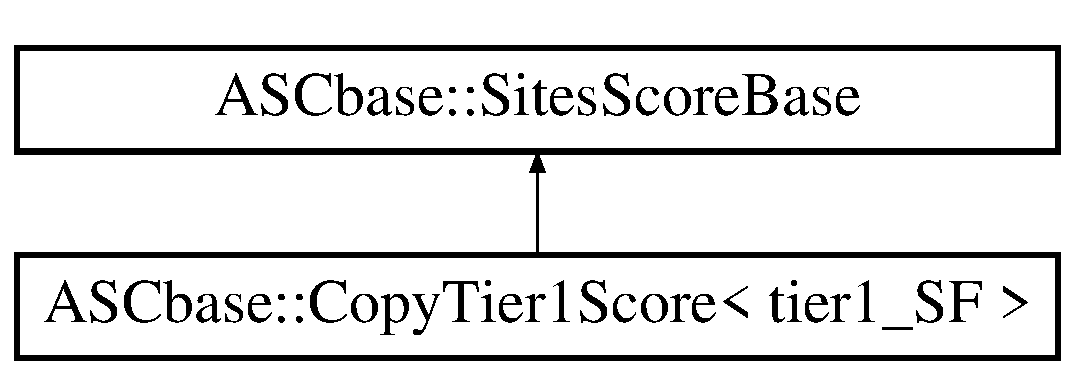
\includegraphics[height=2cm]{classASCbase_1_1CopyTier1Score}
\end{center}
\end{figure}
\subsection*{Public Types}
\begin{CompactItemize}
\item 
typedef tier1\_\-SF::score\_\-cmp \textbf{score\_\-cmp}\label{classASCbase_1_1CopyTier1Score_ded00eb4e145997b1fefe85de8ff6cda}

\end{CompactItemize}
\subsection*{Public Member Functions}
\begin{CompactItemize}
\item 
\bf{Copy\-Tier1Score} ()\label{classASCbase_1_1CopyTier1Score_ff90861b236ad558abc3611850be5eba}

\begin{CompactList}\small\item\em Default constructor for site map point scoring of (aligned) sitemaps. \item\end{CompactList}\item 
\bf{$\sim$Copy\-Tier1Score} ()\label{classASCbase_1_1CopyTier1Score_cc3a6cf33a8c57db5d39627596a4b8d9}

\begin{CompactList}\small\item\em basic destruction \item\end{CompactList}\item 
my\_\-float\_\-t \bf{score} (const \bf{Model\-Sitemap} \&model, const \bf{Dbase\-Sitemap} \&dbase, rigid\_\-align\_\-vi scores)
\begin{CompactList}\small\item\em Returns score from tier1. \item\end{CompactList}\item 
bool \bf{uses\_\-surface\_\-mesh} ()
\item 
bool \bf{uses\_\-hbond\_\-surfaces} ()
\end{CompactItemize}


\subsection{Detailed Description}
\subsubsection*{template$<$class tier1\_\-SF$>$ class ASCbase::Copy\-Tier1Score$<$ tier1\_\-SF $>$}

Returns the tier1 score as the score for the current tier. 

Used to fill in C++ template parameters if we have only 1 tiered scoring

NOTE: the template parameter MUST be the scoring function class used for tier1 



\subsection{Member Function Documentation}
\index{ASCbase::CopyTier1Score@{ASCbase::Copy\-Tier1Score}!score@{score}}
\index{score@{score}!ASCbase::CopyTier1Score@{ASCbase::Copy\-Tier1Score}}
\subsubsection{\setlength{\rightskip}{0pt plus 5cm}template$<$class tier1\_\-SF$>$ my\_\-float\_\-t \bf{ASCbase::Copy\-Tier1Score}$<$ tier1\_\-SF $>$::score (const \bf{Model\-Sitemap} \& {\em model}, const \bf{Dbase\-Sitemap} \& {\em dbase}, rigid\_\-align\_\-vi {\em scores})\hspace{0.3cm}{\tt  [inline]}}\label{classASCbase_1_1CopyTier1Score_d503e8416d1f09bf0c807fd92495e145}


Returns score from tier1. 

\begin{Desc}
\item[Parameters:]
\begin{description}
\item[{\em model}]Const ref to the model site \item[{\em dbase}]Const ref to the sitemap aligned to the model sitemap \item[{\em scores}]iterator to the score data class \end{description}
\end{Desc}
\begin{Desc}
\item[Returns:]score from tier1 (scores-$>$tier1\_\-score) \end{Desc}
\index{ASCbase::CopyTier1Score@{ASCbase::Copy\-Tier1Score}!uses_hbond_surfaces@{uses\_\-hbond\_\-surfaces}}
\index{uses_hbond_surfaces@{uses\_\-hbond\_\-surfaces}!ASCbase::CopyTier1Score@{ASCbase::Copy\-Tier1Score}}
\subsubsection{\setlength{\rightskip}{0pt plus 5cm}template$<$class tier1\_\-SF$>$ bool \bf{ASCbase::Copy\-Tier1Score}$<$ tier1\_\-SF $>$::uses\_\-hbond\_\-surfaces ()\hspace{0.3cm}{\tt  [inline, virtual]}}\label{classASCbase_1_1CopyTier1Score_79790bb098d9f4d8c49951458c155534}


Derived class should return false, unless the derived class is using the hydrogen bond surface caps 

Reimplemented from \bf{ASCbase::Sites\-Score\-Base} \doxyref{p.}{classASCbase_1_1SitesScoreBase_a7a5fcc3e24663874f8066c00089f3cf}.\index{ASCbase::CopyTier1Score@{ASCbase::Copy\-Tier1Score}!uses_surface_mesh@{uses\_\-surface\_\-mesh}}
\index{uses_surface_mesh@{uses\_\-surface\_\-mesh}!ASCbase::CopyTier1Score@{ASCbase::Copy\-Tier1Score}}
\subsubsection{\setlength{\rightskip}{0pt plus 5cm}template$<$class tier1\_\-SF$>$ bool \bf{ASCbase::Copy\-Tier1Score}$<$ tier1\_\-SF $>$::uses\_\-surface\_\-mesh ()\hspace{0.3cm}{\tt  [inline, virtual]}}\label{classASCbase_1_1CopyTier1Score_507e5fdffb914519b624cf87b7470479}


Derived class should return false, unless, the site's surface needs to be to be rotated and translated 

Reimplemented from \bf{ASCbase::Sites\-Score\-Base} \doxyref{p.}{classASCbase_1_1SitesScoreBase_ae4a2a1ae9113bcad0535593c210030f}.

The documentation for this class was generated from the following file:\begin{CompactItemize}
\item 
Copy\-Tier1Score.H\end{CompactItemize}

\section{ASCbase::Dbase\-Sitemap Class Reference}
\label{classASCbase_1_1DbaseSitemap}\index{ASCbase::DbaseSitemap@{ASCbase::DbaseSitemap}}
Create and provide an interface to the database sitemaps.  


{\tt \#include $<$Dbase\-Sitemap.H$>$}

Inheritance diagram for ASCbase::Dbase\-Sitemap::\begin{figure}[H]
\begin{center}
\leavevmode
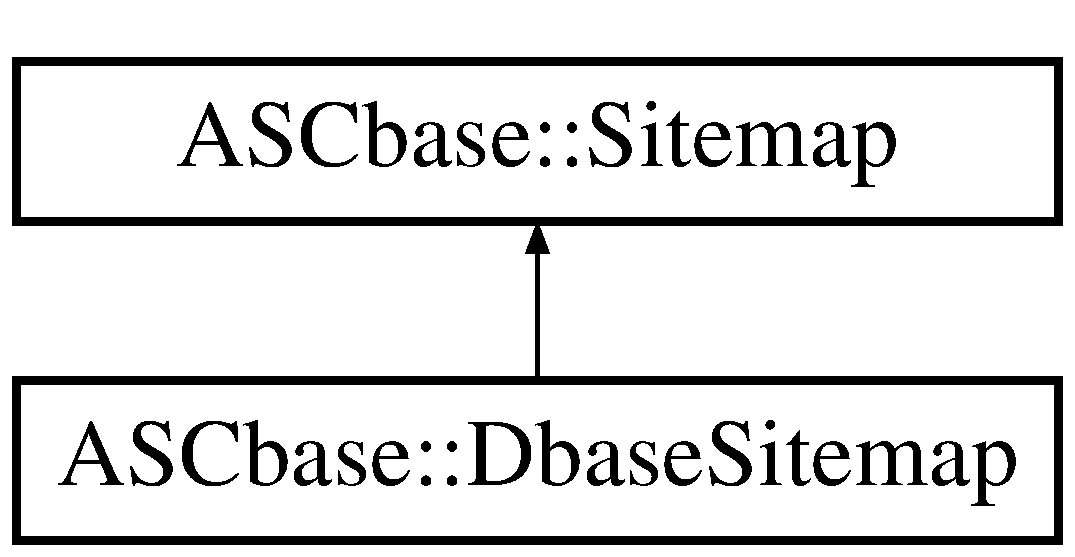
\includegraphics[height=2cm]{classASCbase_1_1DbaseSitemap}
\end{center}
\end{figure}
\subsection*{Public Member Functions}
\begin{CompactItemize}
\item 
\textbf{Dbase\-Sitemap} (const std::string path, const std::string struct\_\-id, const \bf{Base\-Parameters} \&args, const my\_\-float\_\-t max\_\-corr\_\-surf\_\-pt\_\-dist\_\-in=1.5, const bool check\_\-all\_\-triangles=false, const bool load\_\-hbond\_\-surfaces=false)\label{classASCbase_1_1DbaseSitemap_66fdd89eacf2de1b3b682dbb8cd56681}

\item 
const \bf{geometry::Simple\-Trimesh\-Two} \& \textbf{binding\_\-site\_\-mesh\_\-handle} () const \label{classASCbase_1_1DbaseSitemap_6dcc096074247d0908ae2304cd78d5af}

\item 
const my\_\-float\_\-t \textbf{max\_\-corr\_\-surf\_\-pt\_\-dist} () const \label{classASCbase_1_1DbaseSitemap_4e389bea3ac3be5083222a1697a6e7ee}

\end{CompactItemize}
\subsection*{Private Member Functions}
\begin{CompactItemize}
\item 
bool \textbf{load\_\-surface\_\-mesh} (const std::string struct\_\-id, const bool check\_\-all\_\-triangles)\label{classASCbase_1_1DbaseSitemap_6e55d4c66285577dc9a0a0f1db0a1e1a}

\item 
void \bf{clear} ()\label{classASCbase_1_1DbaseSitemap_8ba30a5f3bd0d7efd0310c9b56b3a372}

\begin{CompactList}\small\item\em Frees any allocated objects \& calls \doxyref{init()}{p.}{classASCbase_1_1DbaseSitemap_4ac128bcec4209d070338dd180ec144d} afterwards. \item\end{CompactList}\item 
void \bf{init} ()
\end{CompactItemize}
\subsection*{Private Attributes}
\begin{CompactItemize}
\item 
my\_\-float\_\-t \textbf{A\_\-max\_\-corr\_\-surf\_\-pt\_\-dist}\label{classASCbase_1_1DbaseSitemap_173d970b1d207f6d75d31c3166abed17}

\item 
\bf{geometry::Simple\-Trimesh\-Two} $\ast$ \textbf{A\_\-binding\_\-site\_\-mesh}\label{classASCbase_1_1DbaseSitemap_52c241e9200f7168d030aad6716e046f}

\end{CompactItemize}


\subsection{Detailed Description}
Create and provide an interface to the database sitemaps. 

We need this class because currently the database sitemaps require their surfaces stored using the Immovable\-Trimesh class 



\subsection{Member Function Documentation}
\index{ASCbase::DbaseSitemap@{ASCbase::Dbase\-Sitemap}!init@{init}}
\index{init@{init}!ASCbase::DbaseSitemap@{ASCbase::Dbase\-Sitemap}}
\subsubsection{\setlength{\rightskip}{0pt plus 5cm}void ASCbase::Dbase\-Sitemap::init ()\hspace{0.3cm}{\tt  [inline, private]}}\label{classASCbase_1_1DbaseSitemap_4ac128bcec4209d070338dd180ec144d}


Initializes pointers to 0 and other variables to 0 or another useful value 

Reimplemented from \bf{ASCbase::Sitemap} \doxyref{p.}{classASCbase_1_1Sitemap_2c579b022413645a8ecbdc4317117563}.

The documentation for this class was generated from the following file:\begin{CompactItemize}
\item 
Dbase\-Sitemap.H\end{CompactItemize}

\section{ASCbase::dir\_\-point\_\-storage$<$ \_\-Tp, \_\-Sequence $>$ Class Template Reference}
\label{classASCbase_1_1dir__point__storage}\index{ASCbase::dir_point_storage@{ASCbase::dir\_\-point\_\-storage}}
Storage class for a directed point (point and associated normal direction).  


{\tt \#include $<$dir\_\-point\_\-storage.H$>$}

Inheritance diagram for ASCbase::dir\_\-point\_\-storage$<$ \_\-Tp, \_\-Sequence $>$::\begin{figure}[H]
\begin{center}
\leavevmode
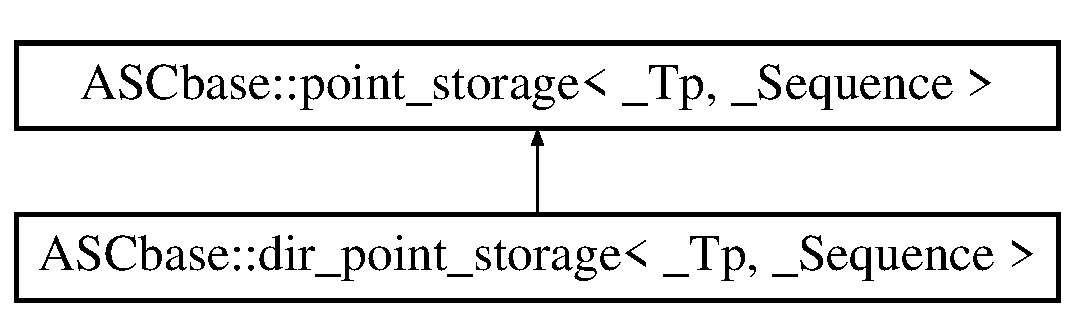
\includegraphics[height=2cm]{classASCbase_1_1dir__point__storage}
\end{center}
\end{figure}
\subsection*{Public Types}
\begin{CompactItemize}
\item 
typedef \_\-Sequence::value\_\-type \textbf{value\_\-type}\label{classASCbase_1_1dir__point__storage_07d6707a6d87d00c05bcd0edc4efc4d7}

\item 
typedef \_\-Sequence::reference \textbf{reference}\label{classASCbase_1_1dir__point__storage_d331bed0bd712e686929cb329241b3bb}

\item 
typedef \_\-Sequence::const\_\-reference \textbf{const\_\-reference}\label{classASCbase_1_1dir__point__storage_bca8c9d13b1a8363a1d9d01f8654ab61}

\item 
typedef \_\-Sequence::iterator \textbf{iterator}\label{classASCbase_1_1dir__point__storage_99f961f57725b54d8c2147a92d01f65b}

\item 
typedef \_\-Sequence::const\_\-iterator \textbf{const\_\-iterator}\label{classASCbase_1_1dir__point__storage_92aae7c0d3854ffca797a683d0954420}

\item 
typedef \_\-Sequence::size\_\-type \textbf{size\_\-type}\label{classASCbase_1_1dir__point__storage_f7f35e9a763d8849e6879f7dd5d93a3f}

\item 
typedef \_\-Sequence \textbf{container\_\-type}\label{classASCbase_1_1dir__point__storage_6a04daea911d059313081e761beec2f1}

\end{CompactItemize}
\subsection*{Public Member Functions}
\begin{CompactItemize}
\item 
\textbf{dir\_\-point\_\-storage} (uint init\_\-num\_\-pts=150, uint stride\_\-in=3)\label{classASCbase_1_1dir__point__storage_8ed74f01bd4c51ec0dbaf60bd61dc736}

\item 
\textbf{dir\_\-point\_\-storage} (const \bf{dir\_\-point\_\-storage} \&src)\label{classASCbase_1_1dir__point__storage_750e00dfd37023bfcd069b90bfeaa586}

\item 
const \bf{dir\_\-point\_\-storage} \& \textbf{operator=} (const \bf{dir\_\-point\_\-storage} \&src)\label{classASCbase_1_1dir__point__storage_0238533e9c171a5c561253af273e1f77}

\item 
const my\_\-float\_\-t $\ast$ \textbf{dirs\_\-begin} () const \label{classASCbase_1_1dir__point__storage_33b13fbfb68925fd3bbe9ebb5bb6e615}

\item 
const my\_\-float\_\-t $\ast$ \textbf{dirs\_\-end} () const \label{classASCbase_1_1dir__point__storage_b5769c55ae99ac2747f5aafe77fc67a1}

\item 
void \bf{push\_\-back} (const value\_\-type \&\_\-\_\-x)
\item 
void \bf{transform} (const my\_\-float\_\-t $\ast$R, const my\_\-float\_\-t $\ast$T)\label{classASCbase_1_1dir__point__storage_b0c2ba79d23e1ff94801a636ffa00709}

\begin{CompactList}\small\item\em Apply a rigid body transformation to the points (current positions). \item\end{CompactList}\item 
void \bf{inverse\_\-transform} (const my\_\-float\_\-t $\ast$R, const my\_\-float\_\-t $\ast$T)\label{classASCbase_1_1dir__point__storage_9c93359e8483342fc61d185dee3c8dde}

\begin{CompactList}\small\item\em Apply a rigid body transformation to the points (current positions). \item\end{CompactList}\item 
void \bf{revert} ()\label{classASCbase_1_1dir__point__storage_c6e015f5121222c68569ae80e5863fc4}

\begin{CompactList}\small\item\em Revert the positions to the original positions. \item\end{CompactList}\item 
void \textbf{set\_\-current\_\-positions\_\-and\_\-directions\_\-as\_\-original} ()\label{classASCbase_1_1dir__point__storage_3e3995a9ff4dd99755198931af1bee9a}

\end{CompactItemize}
\subsection*{Protected Attributes}
\begin{CompactItemize}
\item 
\bf{my\_\-float\_\-array} \textbf{directions}\label{classASCbase_1_1dir__point__storage_cf5010f053b4c87f94175b66ff0fd471}

\end{CompactItemize}
\subsection*{Private Types}
\begin{CompactItemize}
\item 
typedef \_\-Sequence::value\_\-type \textbf{\_\-Sequence\_\-value\_\-type}\label{classASCbase_1_1dir__point__storage_b9764ecb3249fc996e3e10ed78aede2b}

\item 
typedef \bf{point\_\-storage}$<$ \_\-Tp, \_\-Sequence $>$ \textbf{\_\-Base}\label{classASCbase_1_1dir__point__storage_f7b78d6e7f2636f3307999408a6222cb}

\end{CompactItemize}
\subsection*{Private Member Functions}
\begin{CompactItemize}
\item 
\textbf{\_\-\_\-glibcpp\_\-class\_\-requires} (\_\-Tp, \_\-SGIAssignable\-Concept)\label{classASCbase_1_1dir__point__storage_9993616c8c80609852a350e42efc937c}

\item 
\textbf{\_\-\_\-glibcpp\_\-class\_\-requires} (\_\-Sequence, \_\-Back\-Insertion\-Sequence\-Concept)\label{classASCbase_1_1dir__point__storage_47df78f4ab7915ec592d29e28de68b76}

\item 
\textbf{\_\-\_\-glibcpp\_\-class\_\-requires2} (\_\-Tp, \_\-Sequence\_\-value\_\-type, \_\-Same\-Type\-Concept)\label{classASCbase_1_1dir__point__storage_bcfe93369f849040b5d4522ffde3c8cb}

\item 
void \textbf{do\_\-copy} (const \bf{dir\_\-point\_\-storage} \&src)\label{classASCbase_1_1dir__point__storage_54c5c838bba3e21b6ab30f67c89097b7}

\end{CompactItemize}


\subsection{Detailed Description}
\subsubsection*{template$<$typename \_\-Tp, typename \_\-Sequence = std::vector$<$\_\-Tp$>$$>$ class ASCbase::dir\_\-point\_\-storage$<$ \_\-Tp, \_\-Sequence $>$}

Storage class for a directed point (point and associated normal direction). 



\subsection{Member Function Documentation}
\index{ASCbase::dir_point_storage@{ASCbase::dir\_\-point\_\-storage}!push_back@{push\_\-back}}
\index{push_back@{push\_\-back}!ASCbase::dir_point_storage@{ASCbase::dir\_\-point\_\-storage}}
\subsubsection{\setlength{\rightskip}{0pt plus 5cm}template$<$typename \_\-Tp, typename \_\-Sequence = std::vector$<$\_\-Tp$>$$>$ void \bf{ASCbase::dir\_\-point\_\-storage}$<$ \_\-Tp, \_\-Sequence $>$::push\_\-back (const value\_\-type \& {\em \_\-\_\-x})\hspace{0.3cm}{\tt  [inline]}}\label{classASCbase_1_1dir__point__storage_d01a90e5412d2c160cfd4f567d710c4e}


Push an element on the back of the container -- updating the position pointers if the points array was resized 

Reimplemented from \bf{ASCbase::point\_\-storage$<$ \_\-Tp, \_\-Sequence $>$} \doxyref{p.}{classASCbase_1_1point__storage_b1e42dc1e766408149125759061291a6}.

The documentation for this class was generated from the following file:\begin{CompactItemize}
\item 
dir\_\-point\_\-storage.H\end{CompactItemize}

\section{ASCbase::dir\_\-point\_\-t Class Reference}
\label{classASCbase_1_1dir__point__t}\index{ASCbase::dir_point_t@{ASCbase::dir\_\-point\_\-t}}
A point and associated direction.  


{\tt \#include $<$dir\_\-point.H$>$}

Inheritance diagram for ASCbase::dir\_\-point\_\-t::\begin{figure}[H]
\begin{center}
\leavevmode
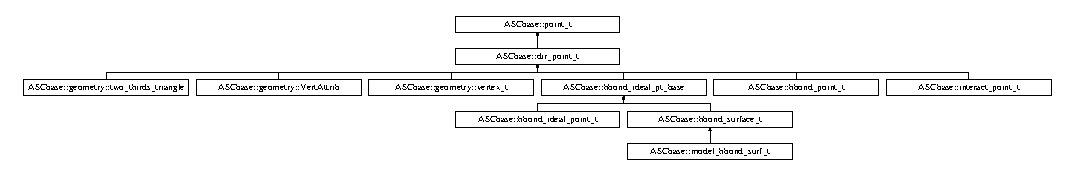
\includegraphics[height=1.92044cm]{classASCbase_1_1dir__point__t}
\end{center}
\end{figure}
\subsection*{Public Member Functions}
\begin{CompactItemize}
\item 
\textbf{dir\_\-point\_\-t} (alloc\_\-t a=ALLOC\_\-POSITION)\label{classASCbase_1_1dir__point__t_57018723a8991fa7f47cc485ba6f3d86}

\item 
\textbf{dir\_\-point\_\-t} (const \bf{dir\_\-point\_\-t} \&p)\label{classASCbase_1_1dir__point__t_3931e2347f2aee30a6d72ccdb211c7bb}

\item 
const \bf{dir\_\-point\_\-t} \& \textbf{operator=} (const \bf{dir\_\-point\_\-t} \&p)\label{classASCbase_1_1dir__point__t_b45b7d7b83e413955ac14b3ccf2336c4}

\item 
void \textbf{delete\_\-dir} ()\label{classASCbase_1_1dir__point__t_dfb4e224f9037f3e14101f5098d5a6c8}

\end{CompactItemize}
\subsection*{Public Attributes}
\begin{CompactItemize}
\item 
my\_\-float\_\-t $\ast$ \textbf{dir}\label{classASCbase_1_1dir__point__t_7378ba825067f07353f214941ca4a715}

\end{CompactItemize}
\subsection*{Private Member Functions}
\begin{CompactItemize}
\item 
void \textbf{do\_\-copy} (const \bf{dir\_\-point\_\-t} \&p)\label{classASCbase_1_1dir__point__t_80fca05c410b767d5eff066f3e5708bd}

\end{CompactItemize}
\subsection*{Private Attributes}
\begin{CompactItemize}
\item 
alloc\_\-t \textbf{\_\-dir\_\-allocated}\label{classASCbase_1_1dir__point__t_14646e021c9e24eedf8a41ef4f6dc68d}

\end{CompactItemize}


\subsection{Detailed Description}
A point and associated direction. 



The documentation for this class was generated from the following file:\begin{CompactItemize}
\item 
dir\_\-point.H\end{CompactItemize}

\section{ASCbase::Discrete\-Sphere Class Reference}
\label{classASCbase_1_1DiscreteSphere}\index{ASCbase::DiscreteSphere@{ASCbase::DiscreteSphere}}
{\tt \#include $<$Discrete\-Sphere.H$>$}

\subsection*{Public Member Functions}
\begin{CompactItemize}
\item 
\bf{Discrete\-Sphere} (sphere\_\-sample\_\-level\_\-t lvl=DISCRETE\_\-SPHERE\_\-LEVEL\_\-TWO)\label{classASCbase_1_1DiscreteSphere_e621966eb3054dab3f2f9798bca76a6b}

\begin{CompactList}\small\item\em Cstor; sets the sphere level. \item\end{CompactList}\item 
\bf{Discrete\-Sphere} (const \bf{Discrete\-Sphere} \&src, const my\_\-float\_\-t $\ast$R, const my\_\-float\_\-t $\ast$T)\label{classASCbase_1_1DiscreteSphere_d712606834a92c7735f3522a9c1983dc}

\begin{CompactList}\small\item\em Apply the given transformation to the copy. \item\end{CompactList}\item 
\bf{$\sim$Discrete\-Sphere} ()\label{classASCbase_1_1DiscreteSphere_0e4e024bf87c9f629c58e96e405a48e9}

\begin{CompactList}\small\item\em Basic Dstor. \item\end{CompactList}\item 
void \bf{scale} (my\_\-float\_\-t s)\label{classASCbase_1_1DiscreteSphere_499dd540bc049f849618e63141a762c9}

\begin{CompactList}\small\item\em Scale the current sphere by s. \item\end{CompactList}\item 
const my\_\-float\_\-t $\ast$ \bf{pts\_\-begin} () const \label{classASCbase_1_1DiscreteSphere_cc1900a41dc02c937dee4964eb40f805}

\begin{CompactList}\small\item\em Get a constant pointer to the first element of the sphere. \item\end{CompactList}\item 
const my\_\-float\_\-t $\ast$ \bf{pts\_\-end} () const \label{classASCbase_1_1DiscreteSphere_19c0f6e97d7235647271a5376dec43c6}

\begin{CompactList}\small\item\em Get a constant pointer to 1 past the last element of the sphere. \item\end{CompactList}\item 
const uint \bf{num\_\-pts} () const \label{classASCbase_1_1DiscreteSphere_f3062c3c256ce124eae95a440cd385d0}

\begin{CompactList}\small\item\em Get the number of points in the array. \item\end{CompactList}\end{CompactItemize}
\subsection*{Private Member Functions}
\begin{CompactItemize}
\item 
void \bf{create\_\-copy} (const my\_\-float\_\-t $\ast$src, my\_\-float\_\-t $\ast$$\ast$dest)\label{classASCbase_1_1DiscreteSphere_27a44b0af870362405f7ff812e909e02}

\begin{CompactList}\small\item\em Create a nonconstant copy of the points. \item\end{CompactList}\end{CompactItemize}
\subsection*{Private Attributes}
\begin{CompactItemize}
\item 
const my\_\-float\_\-t $\ast$ \bf{A\_\-orig\_\-pts}\label{classASCbase_1_1DiscreteSphere_84eda7819366feacab69b8eca58b90a5}

\begin{CompactList}\small\item\em The first element of original sphere. \item\end{CompactList}\item 
uint \bf{A\_\-num\_\-pts}\label{classASCbase_1_1DiscreteSphere_75720a63fc626c586eab6e8e8342f00b}

\begin{CompactList}\small\item\em Number of points in sphere (array). \item\end{CompactList}\item 
my\_\-float\_\-t $\ast$ \bf{A\_\-pts}\label{classASCbase_1_1DiscreteSphere_6fa35750d9d3be1543df6e5fe88efa66}

\begin{CompactList}\small\item\em Pointer to first coord of first pt. \item\end{CompactList}\item 
my\_\-float\_\-t \bf{A\_\-center} [3]\label{classASCbase_1_1DiscreteSphere_c38903731c1e07ab1b6a72aba830abfb}

\begin{CompactList}\small\item\em Center of the sphere. \item\end{CompactList}\end{CompactItemize}
\subsection*{Static Private Attributes}
\begin{CompactItemize}
\item 
static const uint \bf{level\_\-0\_\-len} = 10\label{classASCbase_1_1DiscreteSphere_272db3a33db89cfda38c0a2f7e488bca}

\begin{CompactList}\small\item\em Number of points in the 0th level rep. \item\end{CompactList}\item 
static const uint \bf{level\_\-1\_\-len} = 18\label{classASCbase_1_1DiscreteSphere_f067998b14bfba388d2f803330d6792c}

\begin{CompactList}\small\item\em Number of points in the 1st level rep. \item\end{CompactList}\item 
static const uint \bf{level\_\-2\_\-len} = 26\label{classASCbase_1_1DiscreteSphere_59d0d77b116b29ec295f48add6fec024}

\begin{CompactList}\small\item\em Number of points in the 2nd level rep. \item\end{CompactList}\item 
static const uint \bf{level\_\-3\_\-len} = 39\label{classASCbase_1_1DiscreteSphere_066b8e66f73f541fb02b82ed853a3aed}

\begin{CompactList}\small\item\em Number of points in the 3rd level rep. \item\end{CompactList}\item 
static const my\_\-float\_\-t \bf{level\_\-0} [$\,$]
\begin{CompactList}\small\item\em 0th level rep of 1 (A) sphere \item\end{CompactList}\item 
static const my\_\-float\_\-t \bf{level\_\-1} [$\,$]
\begin{CompactList}\small\item\em 1st level rep of 1 (A) sphere \item\end{CompactList}\item 
static const my\_\-float\_\-t \bf{level\_\-2} [$\,$]
\begin{CompactList}\small\item\em 2nd level rep of 1 (A) sphere \item\end{CompactList}\item 
static const my\_\-float\_\-t \bf{level\_\-3} [$\,$]\label{classASCbase_1_1DiscreteSphere_a074b8dd69e55ae9ac9020e3d5a56a7d}

\begin{CompactList}\small\item\em 3rd level rep of 1 (A) sphere \item\end{CompactList}\end{CompactItemize}


\subsection{Detailed Description}
The method used to generate the 4 sets of points is given in the reference: Kurihara, Yoshio, \char`\"{}Numerical integration of the primitive equations on a spherical grid\char`\"{}, MONTHLY WEATHER REVIEW, 93(7), July, 1965.

The discrete spheres were generated by starting with a base representation of 10 points (level 0). The approximate distance between points was reduced till additional points appeared. This was repeated twice more to obtain the 4 levels of discrete sampling of a sphere with 1 (A) radius centered at the origin (0,0,0).

One nicety is that the points in level 1 correspond to the same points as those generated by starting with 2 (square) pyramids to represent a sphere, (octahedron) halving each original edge and pushing each additional point out till it sits on the sphere. 



\subsection{Member Data Documentation}
\index{ASCbase::DiscreteSphere@{ASCbase::Discrete\-Sphere}!level_0@{level\_\-0}}
\index{level_0@{level\_\-0}!ASCbase::DiscreteSphere@{ASCbase::Discrete\-Sphere}}
\subsubsection{\setlength{\rightskip}{0pt plus 5cm}const my\_\-float\_\-t \bf{Discrete\-Sphere::level\_\-0}\hspace{0.3cm}{\tt  [static, private]}}\label{classASCbase_1_1DiscreteSphere_53fc82a740852de5f8b12e96487c6e90}


\textbf{Initial value:}

\begin{Code}\begin{verbatim} { 0.000000, 1.000000, 0.000000,
                                               0.866025, 0.500000, 0.000000,
                                               0.000000, 0.500000, 0.866025,
                                              -0.866025, 0.500000, 0.000000,
                                              -0.000000, 0.500000, -0.866025,
                                               0.000000, -1.000000, 0.000000,
                                               0.866025, -0.500000, 0.000000,
                                               0.000000, -0.500000, -0.866025,
                                              -0.866025, -0.500000, -0.000000,
                                              -0.000000, -0.500000, 0.866025}
\end{verbatim}\end{Code}
0th level rep of 1 (A) sphere 

\index{ASCbase::DiscreteSphere@{ASCbase::Discrete\-Sphere}!level_1@{level\_\-1}}
\index{level_1@{level\_\-1}!ASCbase::DiscreteSphere@{ASCbase::Discrete\-Sphere}}
\subsubsection{\setlength{\rightskip}{0pt plus 5cm}const my\_\-float\_\-t \bf{Discrete\-Sphere::level\_\-1}\hspace{0.3cm}{\tt  [static, private]}}\label{classASCbase_1_1DiscreteSphere_d3ff32a1e85a1c1f1e321fd09b0ec050}


\textbf{Initial value:}

\begin{Code}\begin{verbatim} { 0.000000, 1.000000, 0.000000,
                                               0.707107, 0.707107, 0.000000,
                                               0.000000, 0.707107, 0.707107,
                                              -0.707107, 0.707107, 0.000000,
                                              -0.000000, 0.707107, -0.707107,
                                               0.707107, 0.000000, 0.707107,
                                               0.000000, 0.000000, 1.000000,
                                              -0.707107, 0.000000, 0.707107,
                                               0.000000, -1.000000, 0.000000,
                                               0.707107, -0.707107, 0.000000,
                                               0.000000, -0.707107, -0.707107,
                                              -0.707107, -0.707107, -0.000000,
                                              -0.000000, -0.707107, 0.707107,
                                               0.707107, 0.000000, -0.707107,
                                               0.000000, 0.000000, -1.000000,
                                              -0.707107, 0.000000, -0.707107,
                                               1.000000, 0.000000, 0.000000,
                                              -1.000000, 0.000000, 0.000000}
\end{verbatim}\end{Code}
1st level rep of 1 (A) sphere 

\index{ASCbase::DiscreteSphere@{ASCbase::Discrete\-Sphere}!level_2@{level\_\-2}}
\index{level_2@{level\_\-2}!ASCbase::DiscreteSphere@{ASCbase::Discrete\-Sphere}}
\subsubsection{\setlength{\rightskip}{0pt plus 5cm}const my\_\-float\_\-t \bf{Discrete\-Sphere::level\_\-2}\hspace{0.3cm}{\tt  [static, private]}}\label{classASCbase_1_1DiscreteSphere_e3e514caf92b337aae7cb629d90f9a61}


\textbf{Initial value:}

\begin{Code}\begin{verbatim} { 0.000000, 1.000000, 0.000000,
                                               0.587785, 0.809017, 0.000000,
                                               0.951057, 0.309017, 0.000000,
                                               0.000000, 0.809017, 0.587785,
                                              -0.587785, 0.809017, 0.000000,
                                              -0.000000, 0.809017, -0.587785,
                                               0.672499, 0.309017, 0.672499,
                                               0.000000, 0.309017, 0.951057,
                                              -0.672499, 0.309017, 0.672499,
                                              -0.951057, 0.309017, 0.000000,
                                              -0.672499, 0.309017, -0.672499,
                                              -0.000000, 0.309017, -0.951057,
                                               0.672499, 0.309017, -0.672499,
                                               0.000000, -1.000000, 0.000000,
                                               0.587785, -0.809017, 0.000000,
                                               0.951057, -0.309017, 0.000000,
                                               0.000000, -0.809017, -0.587785,
                                              -0.587785, -0.809017, -0.000000,
                                              -0.000000, -0.809017, 0.587785,
                                               0.672499, -0.309017, -0.672499,
                                               0.000000, -0.309017, -0.951057,
                                              -0.672499, -0.309017, -0.672499,
                                              -0.951057, -0.309017, -0.000000,
                                              -0.672499, -0.309017, 0.672499,
                                              -0.000000, -0.309017, 0.951057,
                                               0.672499, -0.309017, 0.672499}
\end{verbatim}\end{Code}
2nd level rep of 1 (A) sphere 



The documentation for this class was generated from the following files:\begin{CompactItemize}
\item 
Discrete\-Sphere.H\item 
Discrete\-Sphere.C\end{CompactItemize}

\section{ASCbase::geometry::Distance\-Array Class Reference}
\label{classASCbase_1_1geometry_1_1DistanceArray}\index{ASCbase::geometry::DistanceArray@{ASCbase::geometry::DistanceArray}}
{\tt \#include $<$Distance\-Array.H$>$}

\subsection*{Public Types}
\begin{CompactItemize}
\item 
typedef std::vector$<$ std::vector$<$ const my\_\-float\_\-t $\ast$ $>$ $>$ \textbf{bin\_\-vec}\label{classASCbase_1_1geometry_1_1DistanceArray_c997ffd8bddac3ff42c7dbc23c39e47d}

\item 
typedef bin\_\-vec::const\_\-iterator \textbf{bin\_\-vci}\label{classASCbase_1_1geometry_1_1DistanceArray_4a9a352c0bef59cc6afd3288b7465c8c}

\item 
typedef std::multimap$<$ bin\_\-vci, const my\_\-float\_\-t $\ast$ $>$ \textbf{bin2vert\_\-mmap}\label{classASCbase_1_1geometry_1_1DistanceArray_60d957c24874b08bca3c6e3f00a09ce5}

\item 
typedef bin2vert\_\-mmap::const\_\-iterator \textbf{bin2vert\_\-mmci}\label{classASCbase_1_1geometry_1_1DistanceArray_ec84c66a10ac537a7e6f84c1d558224e}

\end{CompactItemize}
\subsection*{Public Member Functions}
\begin{CompactItemize}
\item 
\bf{Distance\-Array} ()
\item 
\textbf{Distance\-Array} (const my\_\-float\_\-t $\ast$positions, const uint num\_\-pos, const my\_\-float\_\-t bin\_\-width, const my\_\-float\_\-t max\_\-dist)\label{classASCbase_1_1geometry_1_1DistanceArray_3838bfe2441f1dd98f87689aea5cf16a}

\item 
void \textbf{setup\_\-grid} (const my\_\-float\_\-t $\ast$positions, const uint num\_\-pos, const my\_\-float\_\-t bin\_\-width, const my\_\-float\_\-t max\_\-dist)\label{classASCbase_1_1geometry_1_1DistanceArray_501f917f566d2ae25bb0649db73e7625}

\item 
void \textbf{get\_\-min\_\-max\_\-coords} (const my\_\-float\_\-t $\ast$positions, const uint num\_\-pos, my\_\-float\_\-t $\ast$min\_\-pos, my\_\-float\_\-t $\ast$max\_\-pos)\label{classASCbase_1_1geometry_1_1DistanceArray_43c86d0510bafc7dc0cac5b2cba570a7}

\item 
void \textbf{determine\_\-space} (const my\_\-float\_\-t $\ast$min\_\-pos, const my\_\-float\_\-t $\ast$max\_\-pos, my\_\-float\_\-t $\ast$min\_\-corner, my\_\-float\_\-t $\ast$max\_\-corner, int $\ast$num\_\-bins)\label{classASCbase_1_1geometry_1_1DistanceArray_a4cc0a8c9a2b2474b11a3b0ed4c5bedd}

\item 
void \textbf{populate\_\-grid} (const my\_\-float\_\-t $\ast$positions, const uint num\_\-pos, const my\_\-float\_\-t max\_\-dist, std::vector$<$ std::vector$<$ const my\_\-float\_\-t $\ast$ $>$ $>$ $\ast$bins)\label{classASCbase_1_1geometry_1_1DistanceArray_4c9b723809adef008c0b4ca51774f726}

\item 
bin\_\-vci \textbf{get\_\-bin} (const my\_\-float\_\-t $\ast$pt) const \label{classASCbase_1_1geometry_1_1DistanceArray_98eb2f3e69db33ab79650d39da540ebf}

\item 
void \textbf{get\_\-bins} (const my\_\-float\_\-t $\ast$vert\_\-begin, const uint num\_\-vert, bin2vert\_\-mmap $\ast$pts\_\-in\_\-bins) const \label{classASCbase_1_1geometry_1_1DistanceArray_d78373acb3f5018b62772ecb9668c20f}

\item 
bin\_\-vci \bf{bins\_\-end} () const \label{classASCbase_1_1geometry_1_1DistanceArray_c287afc60a8d74ad4123b0e6a8f54eea}

\begin{CompactList}\small\item\em Constant iterator to one past the last bin in the vector. \item\end{CompactList}\end{CompactItemize}
\subsection*{Private Member Functions}
\begin{CompactItemize}
\item 
void \textbf{init} ()\label{classASCbase_1_1geometry_1_1DistanceArray_2750d605e1e1559a1af94773627ebf7e}

\end{CompactItemize}
\subsection*{Private Attributes}
\begin{CompactItemize}
\item 
my\_\-float\_\-t \bf{A\_\-max\_\-dist}\label{classASCbase_1_1geometry_1_1DistanceArray_8d48a1538dbd9906eb57f4ee7b366c66}

\begin{CompactList}\small\item\em Maximum distance for grid to be valid. \item\end{CompactList}\item 
my\_\-float\_\-t \bf{A\_\-bin\_\-width}\label{classASCbase_1_1geometry_1_1DistanceArray_3db71eff2a24debe8bbcfae462759b76}

\begin{CompactList}\small\item\em Side length of a bin. \item\end{CompactList}\item 
my\_\-float\_\-t \bf{A\_\-bin\_\-width\_\-inv}\label{classASCbase_1_1geometry_1_1DistanceArray_87ff0d438ee6643277aa4264f450cd0c}

\begin{CompactList}\small\item\em multiplicative inverse (1 over) side length \item\end{CompactList}\item 
my\_\-float\_\-t \textbf{A\_\-upper\_\-corner} [3]\label{classASCbase_1_1geometry_1_1DistanceArray_01a14247bcabaecf8e917b8aa5acf65a}

\item 
my\_\-float\_\-t \textbf{A\_\-lower\_\-corner} [3]\label{classASCbase_1_1geometry_1_1DistanceArray_8e955d0b3ebfb53e2ca6c19ee8983a29}

\item 
int \textbf{A\_\-num\_\-bins} [3]\label{classASCbase_1_1geometry_1_1DistanceArray_fbbb787940946323d4451b72fcedbfcf}

\item 
bin\_\-vec \textbf{A\_\-bins}\label{classASCbase_1_1geometry_1_1DistanceArray_d1d1803122cc7bfd7cce80e64afe297e}

\item 
bool \textbf{A\_\-bins\_\-are\_\-setup}\label{classASCbase_1_1geometry_1_1DistanceArray_2d5a5de8383858eddee83da5ad46887e}

\end{CompactItemize}


\subsection{Detailed Description}
Make this a simple class to get it workiing -- then template it for generic associated datatype(s) -- keep all functions here for now because if we use templates gcc requires them in header anyhow 



\subsection{Constructor \& Destructor Documentation}
\index{ASCbase::geometry::DistanceArray@{ASCbase::geometry::Distance\-Array}!DistanceArray@{DistanceArray}}
\index{DistanceArray@{DistanceArray}!ASCbase::geometry::DistanceArray@{ASCbase::geometry::Distance\-Array}}
\subsubsection{\setlength{\rightskip}{0pt plus 5cm}ASCbase::geometry::Distance\-Array::Distance\-Array ()\hspace{0.3cm}{\tt  [inline]}}\label{classASCbase_1_1geometry_1_1DistanceArray_2c29de984a15b6bd3269988d1296667b}


Default constructor -- sometimes the array cannot be constructed at class construction 

The documentation for this class was generated from the following file:\begin{CompactItemize}
\item 
Distance\-Array.H\end{CompactItemize}

\section{ASCbase::geometry::Distance\-Array2 Class Reference}
\label{classASCbase_1_1geometry_1_1DistanceArray2}\index{ASCbase::geometry::DistanceArray2@{ASCbase::geometry::DistanceArray2}}
{\tt \#include $<$Distance\-Array2.H$>$}

\subsection*{Public Types}
\begin{CompactItemize}
\item 
typedef std::vector$<$ std::vector$<$ const my\_\-float\_\-t $\ast$ $>$ $>$ \textbf{bin\_\-vec}\label{classASCbase_1_1geometry_1_1DistanceArray2_5671c6bffbec6d424869132a9b8278fe}

\item 
typedef bin\_\-vec::iterator \textbf{bin\_\-vi}\label{classASCbase_1_1geometry_1_1DistanceArray2_3b8950a2f913a1c99f07cd8207b8d4c7}

\item 
typedef bin\_\-vec::const\_\-iterator \textbf{bin\_\-vci}\label{classASCbase_1_1geometry_1_1DistanceArray2_edfb950bc7209814dc46236e34e2dc31}

\item 
typedef std::multimap$<$ bin\_\-vci, const my\_\-float\_\-t $\ast$ $>$ \textbf{bin2vert\_\-mmap}\label{classASCbase_1_1geometry_1_1DistanceArray2_1cb8df28537da9c452689b0424c4f38b}

\item 
typedef bin2vert\_\-mmap::const\_\-iterator \textbf{bin2vert\_\-mmci}\label{classASCbase_1_1geometry_1_1DistanceArray2_0e789f5551c49ffa057399daf777fb66}

\end{CompactItemize}
\subsection*{Public Member Functions}
\begin{CompactItemize}
\item 
\bf{Distance\-Array2} ()
\item 
\textbf{Distance\-Array2} (const my\_\-float\_\-t $\ast$positions, const uint num\_\-pos, const my\_\-float\_\-t bin\_\-width)\label{classASCbase_1_1geometry_1_1DistanceArray2_49275693a93f9cebda96761d3a2915b5}

\item 
void \textbf{setup\_\-grid} (const my\_\-float\_\-t $\ast$positions, const uint num\_\-pos, const my\_\-float\_\-t bin\_\-width)\label{classASCbase_1_1geometry_1_1DistanceArray2_23d27799b8d0236ec7c24c9997922a99}

\item 
void \textbf{get\_\-min\_\-max\_\-coords} (const my\_\-float\_\-t $\ast$positions, const uint num\_\-pos, my\_\-float\_\-t $\ast$min\_\-pos, my\_\-float\_\-t $\ast$max\_\-pos)\label{classASCbase_1_1geometry_1_1DistanceArray2_9bc747ee3e49df4d6ffebb44894e7fc2}

\item 
void \textbf{determine\_\-space} (const my\_\-float\_\-t $\ast$min\_\-pos, const my\_\-float\_\-t $\ast$max\_\-pos, my\_\-float\_\-t $\ast$min\_\-corner, my\_\-float\_\-t $\ast$max\_\-corner, int $\ast$num\_\-bins)\label{classASCbase_1_1geometry_1_1DistanceArray2_d44944a03efc076969d8ab6b9973606c}

\item 
void \textbf{populate\_\-grid} (const my\_\-float\_\-t $\ast$positions, const uint num\_\-pos, const my\_\-float\_\-t bin\_\-width, std::vector$<$ std::vector$<$ const my\_\-float\_\-t $\ast$ $>$ $>$ $\ast$bins)\label{classASCbase_1_1geometry_1_1DistanceArray2_c518041203193931e8be215e65d2b5a1}

\item 
bin\_\-vci \textbf{get\_\-bin} (const my\_\-float\_\-t $\ast$pt) const \label{classASCbase_1_1geometry_1_1DistanceArray2_fe1645f8f07c30ac363eb665e0c3c365}

\item 
void \textbf{get\_\-bins} (const my\_\-float\_\-t $\ast$vert\_\-begin, const uint num\_\-vert, bin2vert\_\-mmap $\ast$pts\_\-in\_\-bins) const \label{classASCbase_1_1geometry_1_1DistanceArray2_dd5739ac76526d894efa53e17461a20b}

\item 
bin\_\-vci \bf{bins\_\-end} () const \label{classASCbase_1_1geometry_1_1DistanceArray2_cf50a867e282cb26de29625843288be7}

\begin{CompactList}\small\item\em Constant iterator to one past the last bin in the vector. \item\end{CompactList}\end{CompactItemize}
\subsection*{Private Member Functions}
\begin{CompactItemize}
\item 
void \textbf{init} ()\label{classASCbase_1_1geometry_1_1DistanceArray2_3a6b04a93a64eb5d858d75872809ed87}

\end{CompactItemize}
\subsection*{Private Attributes}
\begin{CompactItemize}
\item 
my\_\-float\_\-t \bf{A\_\-bin\_\-width}\label{classASCbase_1_1geometry_1_1DistanceArray2_46bf43dba80eca2a90354de43f3e090f}

\begin{CompactList}\small\item\em Side length of a bin. \item\end{CompactList}\item 
my\_\-float\_\-t \bf{A\_\-bin\_\-width\_\-inv}\label{classASCbase_1_1geometry_1_1DistanceArray2_d27b3690450da6a8df54915b042e4425}

\begin{CompactList}\small\item\em multiplicative inverse (1 over) side length \item\end{CompactList}\item 
my\_\-float\_\-t \textbf{A\_\-upper\_\-corner} [3]\label{classASCbase_1_1geometry_1_1DistanceArray2_c20120c88fe303758aa644279ceae45f}

\item 
my\_\-float\_\-t \textbf{A\_\-lower\_\-corner} [3]\label{classASCbase_1_1geometry_1_1DistanceArray2_7ec1a3b6cb3fc3c1fd73d8768fab7cfc}

\item 
int \textbf{A\_\-num\_\-bins} [3]\label{classASCbase_1_1geometry_1_1DistanceArray2_da392e2b7b553662d86c53d58e42cb2d}

\item 
bin\_\-vec \textbf{A\_\-bins}\label{classASCbase_1_1geometry_1_1DistanceArray2_358d86ba1f5aef66aa85e514e273ed0c}

\item 
std::vector$<$ int $>$ \textbf{A\_\-current\_\-bin\_\-idz}\label{classASCbase_1_1geometry_1_1DistanceArray2_ee6a02c194abdc0cd4f4c8caa1b7e238}

\item 
bin\_\-vec \textbf{A\_\-bins\_\-for\_\-moved\_\-pts}\label{classASCbase_1_1geometry_1_1DistanceArray2_df002d40101ccf23897a693eaac5084f}

\item 
bool \textbf{A\_\-bins\_\-are\_\-setup}\label{classASCbase_1_1geometry_1_1DistanceArray2_da8e60db90bd4144a04d5016294c2d1e}

\end{CompactItemize}


\subsection{Detailed Description}
The goal of this method is to make things easier to update and hopefully at the same time a bit faster to setup and access 



\subsection{Constructor \& Destructor Documentation}
\index{ASCbase::geometry::DistanceArray2@{ASCbase::geometry::Distance\-Array2}!DistanceArray2@{DistanceArray2}}
\index{DistanceArray2@{DistanceArray2}!ASCbase::geometry::DistanceArray2@{ASCbase::geometry::Distance\-Array2}}
\subsubsection{\setlength{\rightskip}{0pt plus 5cm}ASCbase::geometry::Distance\-Array2::Distance\-Array2 ()\hspace{0.3cm}{\tt  [inline]}}\label{classASCbase_1_1geometry_1_1DistanceArray2_e951f6ba30f7b4868e4b00347f24da0e}


Default constructor -- sometimes the array cannot be constructed at class construction 

The documentation for this class was generated from the following file:\begin{CompactItemize}
\item 
Distance\-Array2.H\end{CompactItemize}

\section{ASCbase::Drug\-Score\-Interface Class Reference}
\label{classASCbase_1_1DrugScoreInterface}\index{ASCbase::DrugScoreInterface@{ASCbase::DrugScoreInterface}}
Base class: wrapper and parser for external scoring functions.  


{\tt \#include $<$Drug\-Score\-Interface.H$>$}

Inheritance diagram for ASCbase::Drug\-Score\-Interface::\begin{figure}[H]
\begin{center}
\leavevmode
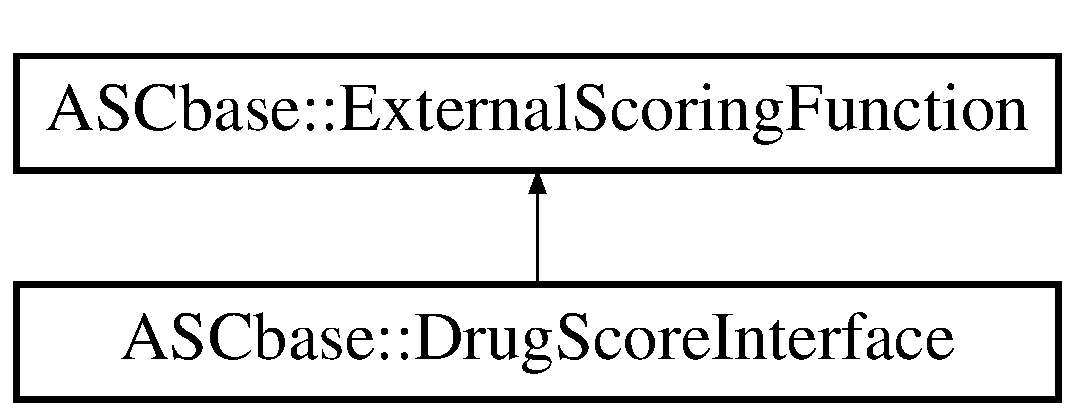
\includegraphics[height=2cm]{classASCbase_1_1DrugScoreInterface}
\end{center}
\end{figure}
\subsection*{Public Member Functions}
\begin{CompactItemize}
\item 
\textbf{Drug\-Score\-Interface} (std::string cmdline)\label{classASCbase_1_1DrugScoreInterface_9e2c6ac97391cc6792e18b9621082b0e}

\item 
\bf{$\sim$Drug\-Score\-Interface} ()\label{classASCbase_1_1DrugScoreInterface_22c88a6abd867ac26771908b5240d710}

\begin{CompactList}\small\item\em Do nothing destructor. \item\end{CompactList}\item 
bool \bf{score} (std::string prot\_\-path, std::string lig\_\-path, std::vector$<$ my\_\-float\_\-t $>$ $\ast$scores)
\begin{CompactList}\small\item\em Wrapper to \doxyref{External\-Scoring\-Function::run}{p.}{classASCbase_1_1ExternalScoringFunction_118e501c983ee3c61747b40741c776ff} and parse output score file. \item\end{CompactList}\item 
void \bf{sf\_\-names} (std::vector$<$ std::string $>$ $\ast$names)
\begin{CompactList}\small\item\em Store the string \char`\"{}Drug\-Score\char`\"{} in names. \item\end{CompactList}\end{CompactItemize}
\subsection*{Static Private Attributes}
\begin{CompactItemize}
\item 
static const std::string \textbf{\_\-fname} = \char`\"{}Drug\-Score\-Interface.C\char`\"{}\label{classASCbase_1_1DrugScoreInterface_7f1e950977fafc985b8678428b3d7ea2}

\end{CompactItemize}


\subsection{Detailed Description}
Base class: wrapper and parser for external scoring functions. 



\subsection{Member Function Documentation}
\index{ASCbase::DrugScoreInterface@{ASCbase::Drug\-Score\-Interface}!score@{score}}
\index{score@{score}!ASCbase::DrugScoreInterface@{ASCbase::Drug\-Score\-Interface}}
\subsubsection{\setlength{\rightskip}{0pt plus 5cm}bool Drug\-Score\-Interface::score (std::string {\em prot\_\-path}, std::string {\em lig\_\-path}, std::vector$<$ my\_\-float\_\-t $>$ $\ast$ {\em scores})\hspace{0.3cm}{\tt  [virtual]}}\label{classASCbase_1_1DrugScoreInterface_dc18368127b62019d1af8c158ba61517}


Wrapper to \doxyref{External\-Scoring\-Function::run}{p.}{classASCbase_1_1ExternalScoringFunction_118e501c983ee3c61747b40741c776ff} and parse output score file. 

Currently is operating under the assumption that PAIR\_\-10 is enough. A change in options would cause the Drug\-Score output files to have a different prefix. Assume the .scr file holds the score only

\begin{Desc}
\item[Parameters:]
\begin{description}
\item[{\em prot\_\-path}]String holding the path of the protein PDB file \item[{\em lig\_\-path}]String holding the path of the ligand mol2 file  scores Pointer to vector to hold the score from Drug\-Score \end{description}
\end{Desc}
\begin{Desc}
\item[Returns:]True if Drug\-Score seemed to work, otherwise false \end{Desc}


Implements \bf{ASCbase::External\-Scoring\-Function} \doxyref{p.}{classASCbase_1_1ExternalScoringFunction_d0e70f7569b5746af85eebc1208afa2a}.\index{ASCbase::DrugScoreInterface@{ASCbase::Drug\-Score\-Interface}!sf_names@{sf\_\-names}}
\index{sf_names@{sf\_\-names}!ASCbase::DrugScoreInterface@{ASCbase::Drug\-Score\-Interface}}
\subsubsection{\setlength{\rightskip}{0pt plus 5cm}void Drug\-Score\-Interface::sf\_\-names (std::vector$<$ std::string $>$ $\ast$ {\em names})\hspace{0.3cm}{\tt  [virtual]}}\label{classASCbase_1_1DrugScoreInterface_f58148608722e9454c2f3e108bfc98f5}


Store the string \char`\"{}Drug\-Score\char`\"{} in names. 

\begin{Desc}
\item[Parameters:]
\begin{description}
\item[{\em names}]Pointer to the vector to write \char`\"{}Drug\-Score\char`\"{} as the first and only scoring function \end{description}
\end{Desc}


Implements \bf{ASCbase::External\-Scoring\-Function} \doxyref{p.}{classASCbase_1_1ExternalScoringFunction_3db07e1e70e4946b507c9b320a124b8b}.

The documentation for this class was generated from the following files:\begin{CompactItemize}
\item 
Drug\-Score\-Interface.H\item 
Drug\-Score\-Interface.C\end{CompactItemize}

\section{ASCbase::Ellipsoidal\-Hbonds\-Score Class Reference}
\label{classASCbase_1_1EllipsoidalHbondsScore}\index{ASCbase::EllipsoidalHbondsScore@{ASCbase::EllipsoidalHbondsScore}}
Base class for scoring rigid alignments of dbase sitemaps to a given model.  


{\tt \#include $<$Ellipsoidal\-Hbonds\-Score.H$>$}

Inheritance diagram for ASCbase::Ellipsoidal\-Hbonds\-Score::\begin{figure}[H]
\begin{center}
\leavevmode
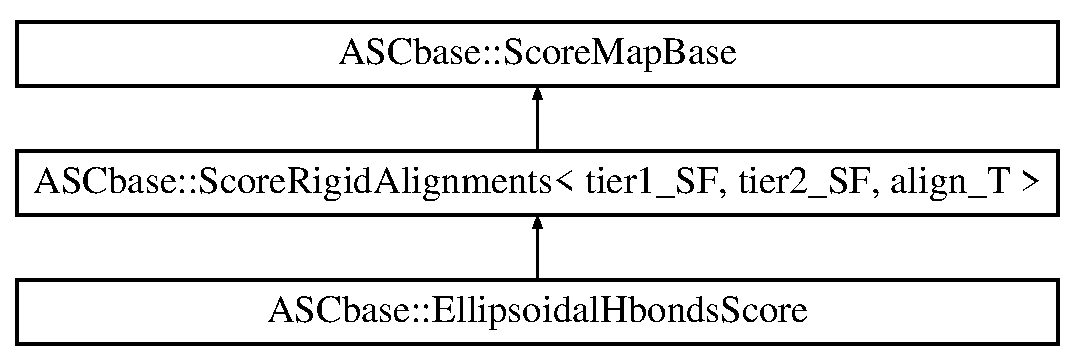
\includegraphics[height=3cm]{classASCbase_1_1EllipsoidalHbondsScore}
\end{center}
\end{figure}
\subsection*{Public Member Functions}
\begin{CompactItemize}
\item 
\bf{Ellipsoidal\-Hbonds\-Score} (\bf{Model\-Sitemap} $\ast$model\_\-in, const \bf{Search\-Parameters} \&params)
\begin{CompactList}\small\item\em Default constructor for scoring methods of rigidly aligned sitemaps. \item\end{CompactList}\item 
\bf{$\sim$Ellipsoidal\-Hbonds\-Score} ()\label{classASCbase_1_1EllipsoidalHbondsScore_4b6b13709f9e3ad4e9402ec26cbef0cd}

\begin{CompactList}\small\item\em basic destruction \item\end{CompactList}\end{CompactItemize}
\subsection*{Protected Member Functions}
\begin{CompactItemize}
\item 
my\_\-float\_\-t \bf{score} (const \bf{Dbase\-Sitemap} \&search, rigid\_\-align\_\-vi scores)
\begin{CompactList}\small\item\em Given an alignment of search to the query, score said alignment. \item\end{CompactList}\item 
my\_\-float\_\-t \textbf{correspondences} (my\_\-float\_\-t $\ast$$\ast$query\_\-pts\_\-ptr, my\_\-float\_\-t $\ast$$\ast$db\_\-pts\_\-ptr, size\_\-t $\ast$npts)\label{classASCbase_1_1EllipsoidalHbondsScore_0a9f3e22c78ef2bcca8664f02a7872f2}

\end{CompactItemize}
\subsection*{Private Member Functions}
\begin{CompactItemize}
\item 
my\_\-float\_\-t \textbf{ellipsoidal\_\-hbonds} (hbond\_\-ideal\_\-pt\_\-vci M, hbond\_\-ideal\_\-pt\_\-vci S)\label{classASCbase_1_1EllipsoidalHbondsScore_861b13badedb987217cec9af4e1195bd}

\end{CompactItemize}
\subsection*{Static Private Attributes}
\begin{CompactItemize}
\item 
static const std::string \bf{\_\-fname} = \char`\"{}Ellipsoidal\-Hbonds\-Score.C\char`\"{}\label{classASCbase_1_1EllipsoidalHbondsScore_5cdf6a4baeab56e974e38792877003f0}

\begin{CompactList}\small\item\em \char`\"{}Ellipsoidal\-Hbonds\-Score.C\char`\"{} \item\end{CompactList}\end{CompactItemize}
\subsection*{Classes}
\begin{CompactItemize}
\item 
struct \textbf{S\_\-and\_\-M}
\end{CompactItemize}


\subsection{Detailed Description}
Base class for scoring rigid alignments of dbase sitemaps to a given model. 



\subsection{Constructor \& Destructor Documentation}
\index{ASCbase::EllipsoidalHbondsScore@{ASCbase::Ellipsoidal\-Hbonds\-Score}!EllipsoidalHbondsScore@{EllipsoidalHbondsScore}}
\index{EllipsoidalHbondsScore@{EllipsoidalHbondsScore}!ASCbase::EllipsoidalHbondsScore@{ASCbase::Ellipsoidal\-Hbonds\-Score}}
\subsubsection{\setlength{\rightskip}{0pt plus 5cm}Ellipsoidal\-Hbonds\-Score::Ellipsoidal\-Hbonds\-Score (\bf{Model\-Sitemap} $\ast$ {\em model\_\-in}, const \bf{Search\-Parameters} \& {\em params})}\label{classASCbase_1_1EllipsoidalHbondsScore_bc22221f61f9d49046c70d382c09100a}


Default constructor for scoring methods of rigidly aligned sitemaps. 

\begin{Desc}
\item[Parameters:]
\begin{description}
\item[{\em model\_\-in}]Pointer to the model points (sitemap class) \item[{\em params}]Reference to the search's runtime parameters \end{description}
\end{Desc}


\subsection{Member Function Documentation}
\index{ASCbase::EllipsoidalHbondsScore@{ASCbase::Ellipsoidal\-Hbonds\-Score}!score@{score}}
\index{score@{score}!ASCbase::EllipsoidalHbondsScore@{ASCbase::Ellipsoidal\-Hbonds\-Score}}
\subsubsection{\setlength{\rightskip}{0pt plus 5cm}my\_\-float\_\-t Ellipsoidal\-Hbonds\-Score::score (const \bf{Dbase\-Sitemap} \& {\em search}, rigid\_\-align\_\-vi {\em scores})\hspace{0.3cm}{\tt  [protected]}}\label{classASCbase_1_1EllipsoidalHbondsScore_d2d7d3b19e1996210beea00d80ca7ec8}


Given an alignment of search to the query, score said alignment. 

\begin{Desc}
\item[Parameters:]
\begin{description}
\item[{\em search}]Pointer to the sitemap aligned to the model sitemap \end{description}
\end{Desc}
\begin{Desc}
\item[Returns:]The score of the alignment \end{Desc}


The documentation for this class was generated from the following files:\begin{CompactItemize}
\item 
Ellipsoidal\-Hbonds\-Score.H\item 
Ellipsoidal\-Hbonds\-Score.C\end{CompactItemize}

\section{ASCbase::External\-Scoring\-Function Class Reference}
\label{classASCbase_1_1ExternalScoringFunction}\index{ASCbase::ExternalScoringFunction@{ASCbase::ExternalScoringFunction}}
Base class: wrapper and parser for external scoring functions.  


{\tt \#include $<$External\-Scoring\-Function.H$>$}

Inheritance diagram for ASCbase::External\-Scoring\-Function::\begin{figure}[H]
\begin{center}
\leavevmode
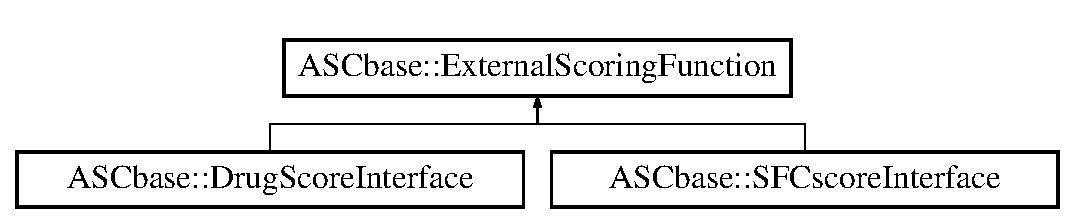
\includegraphics[height=2cm]{classASCbase_1_1ExternalScoringFunction}
\end{center}
\end{figure}
\subsection*{Public Member Functions}
\begin{CompactItemize}
\item 
\bf{External\-Scoring\-Function} (std::string cmdline)
\begin{CompactList}\small\item\em Constructor. \item\end{CompactList}\item 
virtual \bf{$\sim$External\-Scoring\-Function} ()\label{classASCbase_1_1ExternalScoringFunction_c25fb9a4cc68a0608fff4a937fcbf713}

\begin{CompactList}\small\item\em Virtual destruction. \item\end{CompactList}\item 
bool \bf{fail} () const \label{classASCbase_1_1ExternalScoringFunction_e7dd0614a84935bf33ca60bc32fbe2bf}

\begin{CompactList}\small\item\em Determine if calling score will actually do something. \item\end{CompactList}\item 
virtual bool \bf{score} (std::string prot\_\-path, std::string lig\_\-path, std::vector$<$ my\_\-float\_\-t $>$ $\ast$scores)=0
\begin{CompactList}\small\item\em Score protein-ligand pair using chosen external scoring method. \item\end{CompactList}\item 
virtual void \bf{sf\_\-names} (std::vector$<$ std::string $>$ $\ast$names)=0
\begin{CompactList}\small\item\em Get the name(s) of the external scoring function(s) used. \item\end{CompactList}\end{CompactItemize}
\subsection*{Protected Member Functions}
\begin{CompactItemize}
\item 
bool \bf{run} (std::string prot\_\-path, std::string lig\_\-path)
\begin{CompactList}\small\item\em Run the chosen external scoring method. \item\end{CompactList}\end{CompactItemize}
\subsection*{Protected Attributes}
\begin{CompactItemize}
\item 
bool \bf{a\_\-fail}\label{classASCbase_1_1ExternalScoringFunction_2d87c7620eaa9033fcde870432b39485}

\begin{CompactList}\small\item\em True means unable to run or failure occured. \item\end{CompactList}\end{CompactItemize}
\subsection*{Private Attributes}
\begin{CompactItemize}
\item 
std::vector$<$ std::string $>$ \textbf{cmdline\_\-toks}\label{classASCbase_1_1ExternalScoringFunction_4aa21826b34ff982e3924f6f74480bad}

\item 
std::vector$<$ std::string $>$::const\_\-iterator \textbf{prot\_\-str\_\-iter}\label{classASCbase_1_1ExternalScoringFunction_c5c1b5c0cf714978ff2c3b669033c2f0}

\item 
std::vector$<$ std::string $>$::const\_\-iterator \textbf{lig\_\-str\_\-iter}\label{classASCbase_1_1ExternalScoringFunction_9f0e031e5f90ee140083e81ae450ae93}

\end{CompactItemize}


\subsection{Detailed Description}
Base class: wrapper and parser for external scoring functions. 



\subsection{Constructor \& Destructor Documentation}
\index{ASCbase::ExternalScoringFunction@{ASCbase::External\-Scoring\-Function}!ExternalScoringFunction@{ExternalScoringFunction}}
\index{ExternalScoringFunction@{ExternalScoringFunction}!ASCbase::ExternalScoringFunction@{ASCbase::External\-Scoring\-Function}}
\subsubsection{\setlength{\rightskip}{0pt plus 5cm}External\-Scoring\-Function::External\-Scoring\-Function (std::string {\em cmdline})}\label{classASCbase_1_1ExternalScoringFunction_11f4a861421bbc7a766a72b0b6ce3b42}


Constructor. 

\begin{Desc}
\item[Parameters:]
\begin{description}
\item[{\em cmdline}]Command line to run the chosen external protein-ligand scoring function with the variables \$PROTEIN and \$LIGAND denoting where to stuff the values for the proteins and ligands to score. \end{description}
\end{Desc}


\subsection{Member Function Documentation}
\index{ASCbase::ExternalScoringFunction@{ASCbase::External\-Scoring\-Function}!run@{run}}
\index{run@{run}!ASCbase::ExternalScoringFunction@{ASCbase::External\-Scoring\-Function}}
\subsubsection{\setlength{\rightskip}{0pt plus 5cm}bool External\-Scoring\-Function::run (std::string {\em prot\_\-path}, std::string {\em lig\_\-path})\hspace{0.3cm}{\tt  [protected]}}\label{classASCbase_1_1ExternalScoringFunction_118e501c983ee3c61747b40741c776ff}


Run the chosen external scoring method. 

Run the chosen external scoring method \begin{Desc}
\item[Parameters:]
\begin{description}
\item[{\em prot\_\-path}]String holding the path of the protein PDB file \item[{\em lig\_\-path}]String holding the path of the ligand mol2 file \end{description}
\end{Desc}
\begin{Desc}
\item[Returns:]True if prot\_\-path and lig\_\-path exist and are not directories, otherwise false \end{Desc}
\index{ASCbase::ExternalScoringFunction@{ASCbase::External\-Scoring\-Function}!score@{score}}
\index{score@{score}!ASCbase::ExternalScoringFunction@{ASCbase::External\-Scoring\-Function}}
\subsubsection{\setlength{\rightskip}{0pt plus 5cm}virtual bool ASCbase::External\-Scoring\-Function::score (std::string {\em prot\_\-path}, std::string {\em lig\_\-path}, std::vector$<$ my\_\-float\_\-t $>$ $\ast$ {\em scores})\hspace{0.3cm}{\tt  [pure virtual]}}\label{classASCbase_1_1ExternalScoringFunction_d0e70f7569b5746af85eebc1208afa2a}


Score protein-ligand pair using chosen external scoring method. 

Score using chosen external scoring method -- force derived classes to override with their version. \begin{Desc}
\item[Parameters:]
\begin{description}
\item[{\em prot\_\-path}]String holding the path of the protein PDB file \item[{\em lig\_\-path}]String holding the path of the ligand mol2 file \item[{\em scores}]Pointer to vector holding the scores of the pair \end{description}
\end{Desc}
\begin{Desc}
\item[Returns:]True if prot\_\-path and lig\_\-path exist and are not directories, otherwise false \end{Desc}


Implemented in \bf{ASCbase::Drug\-Score\-Interface} \doxyref{p.}{classASCbase_1_1DrugScoreInterface_dc18368127b62019d1af8c158ba61517}, and \bf{ASCbase::SFCscore\-Interface} \doxyref{p.}{classASCbase_1_1SFCscoreInterface_354838006d3b086f93b7245cf0223a70}.\index{ASCbase::ExternalScoringFunction@{ASCbase::External\-Scoring\-Function}!sf_names@{sf\_\-names}}
\index{sf_names@{sf\_\-names}!ASCbase::ExternalScoringFunction@{ASCbase::External\-Scoring\-Function}}
\subsubsection{\setlength{\rightskip}{0pt plus 5cm}virtual void ASCbase::External\-Scoring\-Function::sf\_\-names (std::vector$<$ std::string $>$ $\ast$ {\em names})\hspace{0.3cm}{\tt  [pure virtual]}}\label{classASCbase_1_1ExternalScoringFunction_3db07e1e70e4946b507c9b320a124b8b}


Get the name(s) of the external scoring function(s) used. 

To be overloaded by the derived classes \begin{Desc}
\item[Parameters:]
\begin{description}
\item[{\em names}]Pointer to vector of strings holding the names of the scoring function(s) in the same order as the scores stored in the ext\_\-scores vector in \doxyref{rigid\_\-align\_\-t}{p.}{classASCbase_1_1rigid__align__t} \end{description}
\end{Desc}


Implemented in \bf{ASCbase::Drug\-Score\-Interface} \doxyref{p.}{classASCbase_1_1DrugScoreInterface_f58148608722e9454c2f3e108bfc98f5}, and \bf{ASCbase::SFCscore\-Interface} \doxyref{p.}{classASCbase_1_1SFCscoreInterface_00c2a69a8732cc3eae24ed2bb61dc638}.

The documentation for this class was generated from the following files:\begin{CompactItemize}
\item 
External\-Scoring\-Function.H\item 
External\-Scoring\-Function.C\end{CompactItemize}

\section{ASCbase::geometry::Face\-Attrib Class Reference}
\label{classASCbase_1_1geometry_1_1FaceAttrib}\index{ASCbase::geometry::FaceAttrib@{ASCbase::geometry::FaceAttrib}}
Class to hold the attributes associated with a face.  


{\tt \#include $<$Face\-Attrib.H$>$}

\subsection*{Public Types}
\begin{CompactItemize}
\item 
typedef std::vector$<$ \bf{Face\-Attrib} $>$::iterator \bf{vi}\label{classASCbase_1_1geometry_1_1FaceAttrib_3eb0b75de163c3238b77c100bac7cb63}

\begin{CompactList}\small\item\em Iterator in a vector of faces. \item\end{CompactList}\item 
typedef std::vector$<$ \bf{Face\-Attrib} $>$::const\_\-iterator \bf{vci}\label{classASCbase_1_1geometry_1_1FaceAttrib_842f81a96ce61b0118b03ee349c53bb8}

\begin{CompactList}\small\item\em Const iterater in a vector of faces. \item\end{CompactList}\end{CompactItemize}
\subsection*{Public Member Functions}
\begin{CompactItemize}
\item 
\bf{Face\-Attrib} ()\label{classASCbase_1_1geometry_1_1FaceAttrib_58f47b12a77b0bfe438d4d410a2545bb}

\begin{CompactList}\small\item\em Default constructor. \item\end{CompactList}\item 
\bf{Face\-Attrib} (\bf{Vert\-Attrib::vi} V0, \bf{Vert\-Attrib::vi} V1, \bf{Vert\-Attrib::vi} V2)
\begin{CompactList}\small\item\em Construct using 3 vertices. \item\end{CompactList}\item 
\bf{Face\-Attrib} (const \bf{Face\-Attrib} \&F)\label{classASCbase_1_1geometry_1_1FaceAttrib_1e99d6a0fc70decafa2658c8a51779a1}

\begin{CompactList}\small\item\em Copy constructor. \item\end{CompactList}\item 
const \bf{Face\-Attrib} \& \bf{operator=} (const \bf{Face\-Attrib} \&F)\label{classASCbase_1_1geometry_1_1FaceAttrib_7af2c6ec62751d4207bf11f0daee1649}

\begin{CompactList}\small\item\em Assignment operator. \item\end{CompactList}\item 
void \bf{set\_\-vertices} (\bf{Vert\-Attrib::vi} V0, \bf{Vert\-Attrib::vi} V1, \bf{Vert\-Attrib::vi} V2)
\begin{CompactList}\small\item\em assign the 3 vertices \item\end{CompactList}\item 
void \bf{add\_\-sample\_\-pt} (const my\_\-float\_\-t $\ast$pt)\label{classASCbase_1_1geometry_1_1FaceAttrib_39dedd2a7d3b5d02eb9d1ffc6e7c9d93}

\begin{CompactList}\small\item\em Copy constructor. \item\end{CompactList}\item 
void \textbf{get\_\-other\_\-verts} (const \bf{Vert\-Attrib::vci} V, \bf{Vert\-Attrib::vi} A, \bf{Vert\-Attrib::vi} B)\label{classASCbase_1_1geometry_1_1FaceAttrib_458e3c60431028bc94c74768f5651985}

\item 
void \bf{closest\_\-point} (const my\_\-float\_\-t $\ast$P, const my\_\-float\_\-t prev\_\-best\_\-d, my\_\-float\_\-t $\ast$d, my\_\-float\_\-t $\ast$closest\_\-pt, my\_\-float\_\-t $\ast$corr\_\-N) const 
\begin{CompactList}\small\item\em Get the point on face that is the closest to P. \item\end{CompactList}\item 
bool \bf{barycentric\_\-coords} (const my\_\-float\_\-t $\ast$p, my\_\-float\_\-t $\ast$b) const 
\begin{CompactList}\small\item\em Use the area method to compute barycentric coordinates for p. \item\end{CompactList}\item 
\bf{Face\-Attrib::vi} \bf{next} (\bf{Vert\-Attrib::vi} V) const 
\item 
\bf{Face\-Attrib::vi} \bf{prev} (\bf{Vert\-Attrib::vi} V) const 
\item 
bool \textbf{set\_\-face\_\-neighbor} (\bf{Vert\-Attrib::vi} V0, \bf{Vert\-Attrib::vi} V1, \bf{Face\-Attrib::vi} nbr)\label{classASCbase_1_1geometry_1_1FaceAttrib_412ac3fa3ee7ec5d559c4a15badd5415}

\item 
void \textbf{get\_\-vertices} (\bf{Vert\-Attrib::vi} $\ast$V) const \label{classASCbase_1_1geometry_1_1FaceAttrib_133f30ead168af2a6231f366e21785e9}

\item 
my\_\-float\_\-t \textbf{proj\_\-pt\_\-to\_\-plane} (const my\_\-float\_\-t $\ast$pt, my\_\-float\_\-t $\ast$proj\_\-pt) const \label{classASCbase_1_1geometry_1_1FaceAttrib_7df244a711c3d3aaafcab27567ccb106}

\end{CompactItemize}
\subsection*{Static Public Member Functions}
\begin{CompactItemize}
\item 
static void \textbf{test\_\-removing\_\-edge} (\bf{Vert\-Attrib::vi} $\ast$end\_\-pts, \bf{Face\-Attrib::vi} $\ast$edge\_\-faces, \bf{Vert\-Attrib::vi} verts\_\-begin)\label{classASCbase_1_1geometry_1_1FaceAttrib_aaa21e453271eb9dcc0d7c93b4ebbb8d}

\end{CompactItemize}
\subsection*{Static Public Attributes}
\begin{CompactItemize}
\item 
static std::vector$<$ \bf{Face\-Attrib} $>$ \textbf{NULL\_\-FACES\_\-STORAGE}\label{classASCbase_1_1geometry_1_1FaceAttrib_c9163721e9096e21f15bb26d31bb4aa6}

\item 
static const \bf{Face\-Attrib::vi} \textbf{NULL\_\-VI} = Face\-Attrib::NULL\_\-FACES\_\-STORAGE.end()\label{classASCbase_1_1geometry_1_1FaceAttrib_24cdd7efba12dbdb850dfc048e587494}

\end{CompactItemize}
\subsection*{Private Member Functions}
\begin{CompactItemize}
\item 
void \bf{initialize} ()\label{classASCbase_1_1geometry_1_1FaceAttrib_0a74580eb4b67a2aab807c573f23150f}

\begin{CompactList}\small\item\em Initialize class variables. \item\end{CompactList}\item 
void \textbf{do\_\-copy} (const \bf{Face\-Attrib} \&F)\label{classASCbase_1_1geometry_1_1FaceAttrib_37f47b2aff4f63b97ba3c3925a9ce48c}

\item 
size\_\-t \bf{next\_\-fnei\_\-idx} (\bf{Vert\-Attrib::vi} V) const 
\item 
size\_\-t \bf{prev\_\-fnei\_\-idx} (\bf{Vert\-Attrib::vi} V) const 
\item 
bool \bf{replace\_\-vert} (\bf{Vert\-Attrib::vi} V\_\-old, \bf{Vert\-Attrib::vi} V\_\-new)\label{classASCbase_1_1geometry_1_1FaceAttrib_4ce6b7f01131a4b4cf7f2b0941a06815}

\begin{CompactList}\small\item\em Replace the old vertex with the new vertex. \item\end{CompactList}\item 
bool \bf{not\_\-sharp} (\bf{Vert\-Attrib::vi} A, \bf{Vert\-Attrib::vi} B)\label{classASCbase_1_1geometry_1_1FaceAttrib_0acc4dced66afbc8ab90ed453dbd275e}

\begin{CompactList}\small\item\em Example \char`\"{}sharp\char`\"{} function -- always returns false. \item\end{CompactList}\item 
my\_\-float\_\-t \textbf{E\_\-disc} (\bf{Vert\-Attrib::vi} V\_\-s, \bf{Vert\-Attrib::vi} V\_\-t, \bf{Vert\-Attrib::vi} V\_\-l, \bf{Vert\-Attrib::vi} V\_\-r, bool($\ast$sharp\-Func)(\bf{Vert\-Attrib::vi} A, \bf{Vert\-Attrib::vi} B))\label{classASCbase_1_1geometry_1_1FaceAttrib_5781c0b9abd91d4e0fc90d0e495d7d1d}

\end{CompactItemize}
\subsection*{Static Private Member Functions}
\begin{CompactItemize}
\item 
static bool \bf{get\_\-faces} (const \bf{Vert\-Attrib::vi} \&central\_\-vert, const \bf{Face\-Attrib::vi} \&start\_\-face, std::vector$<$ \bf{Face\-Attrib::vi} $>$ $\ast$faces\_\-out, const bool skip\_\-first\_\-prev=false)
\begin{CompactList}\small\item\em Get all the faces for the given vertex. \item\end{CompactList}\item 
static bool \textbf{get\_\-faces} (\bf{Face\-Attrib::vi} central\_\-face, std::vector$<$ \bf{Face\-Attrib::vi} $>$ $\ast$faces\_\-out)\label{classASCbase_1_1geometry_1_1FaceAttrib_48c6dd9a6f5ee0f205006ac346a8c6db}

\end{CompactItemize}
\subsection*{Private Attributes}
\begin{CompactItemize}
\item 
\bf{Vert\-Attrib::vi} \bf{A\_\-V} [3]\label{classASCbase_1_1geometry_1_1FaceAttrib_904831d51fed8e5ecc419c2f2c55fce4}

\begin{CompactList}\small\item\em Vertices of this face. \item\end{CompactList}\item 
\bf{Face\-Attrib::vi} \bf{A\_\-fnei} [3]\label{classASCbase_1_1geometry_1_1FaceAttrib_194b12426bd69f372dbb37e32fd156e1}

\begin{CompactList}\small\item\em Neighbor faces -- first corresponds to A\_\-V[0] -$>$ A\_\-V[1], ... \item\end{CompactList}\item 
std::vector$<$ const my\_\-float\_\-t $\ast$ $>$ \textbf{A\_\-X}\label{classASCbase_1_1geometry_1_1FaceAttrib_adef9b1294772d0546142c2a8d92b466}

\item 
my\_\-float\_\-t \bf{A\_\-normal} [3]\label{classASCbase_1_1geometry_1_1FaceAttrib_6850d39bcde536959e914a695a977422}

\begin{CompactList}\small\item\em Normal to the face (V[0] - V[1]) x (V[2] - V[1]). \item\end{CompactList}\item 
my\_\-float\_\-t \bf{A\_\-area}\label{classASCbase_1_1geometry_1_1FaceAttrib_e32bb1596b04ad7b14209d60c8d73468}

\begin{CompactList}\small\item\em Area of the face. \item\end{CompactList}\end{CompactItemize}
\subsection*{Friends}
\begin{CompactItemize}
\item 
std::ostream \& \textbf{operator$<$$<$} (std::ostream \&out, const \bf{Face\-Attrib} \&F)\label{classASCbase_1_1geometry_1_1FaceAttrib_c6ae99b680126898fbde7fef3d9afd8a}

\end{CompactItemize}
\subsection*{Classes}
\begin{CompactItemize}
\item 
class \textbf{point\_\-data\_\-t}
\end{CompactItemize}


\subsection{Detailed Description}
Class to hold the attributes associated with a face. 

Note: inside this class I tended to use \doxyref{Face\-Attrib::vi}{p.}{classASCbase_1_1geometry_1_1FaceAttrib_3eb0b75de163c3238b77c100bac7cb63} so that it is clear which vector iterator is being used 



\subsection{Constructor \& Destructor Documentation}
\index{ASCbase::geometry::FaceAttrib@{ASCbase::geometry::Face\-Attrib}!FaceAttrib@{FaceAttrib}}
\index{FaceAttrib@{FaceAttrib}!ASCbase::geometry::FaceAttrib@{ASCbase::geometry::Face\-Attrib}}
\subsubsection{\setlength{\rightskip}{0pt plus 5cm}ASCbase::geometry::Face\-Attrib::Face\-Attrib (\bf{Vert\-Attrib::vi} {\em V0}, \bf{Vert\-Attrib::vi} {\em V1}, \bf{Vert\-Attrib::vi} {\em V2})\hspace{0.3cm}{\tt  [inline]}}\label{classASCbase_1_1geometry_1_1FaceAttrib_defd6241ccd16e32a99aba6767e8b33f}


Construct using 3 vertices. 

Assumption: The vertices are in counter clockwise order so that barycentric method to determine if the projection of a point lies inside the face places the centroid of the face inside. Besides, the right hand rule has been typically followed up to this point

NEED TO THINK ABOUT THIS MORE -- after rotation we could mess up the cross product? If it flips to be clockwise with respect to the right hand rule we should be ok since the resulting vector of the cross products will still face the same direction for all 3 vectors 

\subsection{Member Function Documentation}
\index{ASCbase::geometry::FaceAttrib@{ASCbase::geometry::Face\-Attrib}!barycentric_coords@{barycentric\_\-coords}}
\index{barycentric_coords@{barycentric\_\-coords}!ASCbase::geometry::FaceAttrib@{ASCbase::geometry::Face\-Attrib}}
\subsubsection{\setlength{\rightskip}{0pt plus 5cm}bool Face\-Attrib::barycentric\_\-coords (const my\_\-float\_\-t $\ast$ {\em p}, my\_\-float\_\-t $\ast$ {\em b}) const}\label{classASCbase_1_1geometry_1_1FaceAttrib_12fa38d9657d070bf64725471f209ee8}


Use the area method to compute barycentric coordinates for p. 

Assumption: p lies in the plane defined by the 3 vertices of this face This function constrains the barycentric coordinates to be non-negative, but it does return false if the point is outside of the face. Note that the \char`\"{}outside\char`\"{} is subject to numerical errors and it could potentially be \char`\"{}inside\char`\"{}, but that is irrelavent with respect to the way we currently intend to use this function.

\begin{Desc}
\item[Returns:]True if p is inside this face, false otherwise \end{Desc}
\index{ASCbase::geometry::FaceAttrib@{ASCbase::geometry::Face\-Attrib}!closest_point@{closest\_\-point}}
\index{closest_point@{closest\_\-point}!ASCbase::geometry::FaceAttrib@{ASCbase::geometry::Face\-Attrib}}
\subsubsection{\setlength{\rightskip}{0pt plus 5cm}void Face\-Attrib::closest\_\-point (const my\_\-float\_\-t $\ast$ {\em P}, const my\_\-float\_\-t {\em prev\_\-best\_\-d}, my\_\-float\_\-t $\ast$ {\em d}, my\_\-float\_\-t $\ast$ {\em closest\_\-pt}, my\_\-float\_\-t $\ast$ {\em corr\_\-N}) const}\label{classASCbase_1_1geometry_1_1FaceAttrib_26012b35094ee4eff6f782e21f837f88}


Get the point on face that is the closest to P. 

ASSUMPTION: A\_\-normal is valid! \index{ASCbase::geometry::FaceAttrib@{ASCbase::geometry::Face\-Attrib}!get_faces@{get\_\-faces}}
\index{get_faces@{get\_\-faces}!ASCbase::geometry::FaceAttrib@{ASCbase::geometry::Face\-Attrib}}
\subsubsection{\setlength{\rightskip}{0pt plus 5cm}static bool ASCbase::geometry::Face\-Attrib::get\_\-faces (const \bf{Vert\-Attrib::vi} \& {\em central\_\-vert}, const \bf{Face\-Attrib::vi} \& {\em start\_\-face}, std::vector$<$ \bf{Face\-Attrib::vi} $>$ $\ast$ {\em faces\_\-out}, const bool {\em skip\_\-first\_\-prev} = {\tt false})\hspace{0.3cm}{\tt  [inline, static, private]}}\label{classASCbase_1_1geometry_1_1FaceAttrib_5ae94bb0705521f9ab476ce65b525e83}


Get all the faces for the given vertex. 

This method does not add the starting face First this method will check all the faces that can be found via the face-$>$next links. If a \char`\"{}null\char`\"{} face is found, it will check all the faces via the face-$>$prev links.

This method will fail if the mesh is of poor quality and all of the faces cannot be found by both next and prev traversal \index{ASCbase::geometry::FaceAttrib@{ASCbase::geometry::Face\-Attrib}!next@{next}}
\index{next@{next}!ASCbase::geometry::FaceAttrib@{ASCbase::geometry::Face\-Attrib}}
\subsubsection{\setlength{\rightskip}{0pt plus 5cm}\bf{Face\-Attrib::vi} ASCbase::geometry::Face\-Attrib::next (\bf{Vert\-Attrib::vi} {\em V}) const\hspace{0.3cm}{\tt  [inline]}}\label{classASCbase_1_1geometry_1_1FaceAttrib_8e27be3eedc3330db14d563b0cc829b6}


Return the next face after the current face given a vertex V of the current face -- use right hand rule for next (i.e. counter-clockwise rotation) \index{ASCbase::geometry::FaceAttrib@{ASCbase::geometry::Face\-Attrib}!next_fnei_idx@{next\_\-fnei\_\-idx}}
\index{next_fnei_idx@{next\_\-fnei\_\-idx}!ASCbase::geometry::FaceAttrib@{ASCbase::geometry::Face\-Attrib}}
\subsubsection{\setlength{\rightskip}{0pt plus 5cm}size\_\-t ASCbase::geometry::Face\-Attrib::next\_\-fnei\_\-idx (\bf{Vert\-Attrib::vi} {\em V}) const\hspace{0.3cm}{\tt  [inline, private]}}\label{classASCbase_1_1geometry_1_1FaceAttrib_c214a46fbbbeb51a667c7eb23b2b4916}


Return the next face after the current face given a vertex V of the current face -- use right hand rule for next (i.e. counter-clockwise rotation) \index{ASCbase::geometry::FaceAttrib@{ASCbase::geometry::Face\-Attrib}!prev@{prev}}
\index{prev@{prev}!ASCbase::geometry::FaceAttrib@{ASCbase::geometry::Face\-Attrib}}
\subsubsection{\setlength{\rightskip}{0pt plus 5cm}\bf{Face\-Attrib::vi} ASCbase::geometry::Face\-Attrib::prev (\bf{Vert\-Attrib::vi} {\em V}) const\hspace{0.3cm}{\tt  [inline]}}\label{classASCbase_1_1geometry_1_1FaceAttrib_48d587e02fec7b05c076bbd2c9c75467}


Return the previous face before the current face given a vertex V of the current face -- use right hand rule for previou (i.e. clockwise rotation) \index{ASCbase::geometry::FaceAttrib@{ASCbase::geometry::Face\-Attrib}!prev_fnei_idx@{prev\_\-fnei\_\-idx}}
\index{prev_fnei_idx@{prev\_\-fnei\_\-idx}!ASCbase::geometry::FaceAttrib@{ASCbase::geometry::Face\-Attrib}}
\subsubsection{\setlength{\rightskip}{0pt plus 5cm}size\_\-t ASCbase::geometry::Face\-Attrib::prev\_\-fnei\_\-idx (\bf{Vert\-Attrib::vi} {\em V}) const\hspace{0.3cm}{\tt  [inline, private]}}\label{classASCbase_1_1geometry_1_1FaceAttrib_14c4e75eb1b55664d343ee816b6899fd}


Return the previous face before the current face given a vertex V of the current face -- use right hand rule for previous (i.e. clockwise rotation) \index{ASCbase::geometry::FaceAttrib@{ASCbase::geometry::Face\-Attrib}!set_vertices@{set\_\-vertices}}
\index{set_vertices@{set\_\-vertices}!ASCbase::geometry::FaceAttrib@{ASCbase::geometry::Face\-Attrib}}
\subsubsection{\setlength{\rightskip}{0pt plus 5cm}void ASCbase::geometry::Face\-Attrib::set\_\-vertices (\bf{Vert\-Attrib::vi} {\em V0}, \bf{Vert\-Attrib::vi} {\em V1}, \bf{Vert\-Attrib::vi} {\em V2})\hspace{0.3cm}{\tt  [inline]}}\label{classASCbase_1_1geometry_1_1FaceAttrib_fa71741b951f0b895f21c0322ba53dc2}


assign the 3 vertices 

Assumption: The vertices are in counter clockwise order so that barycentric method to determine if the projection of a point lies inside the face places the centroid of the face inside. Besides, the right hand rule has been typically followed up to this point 

The documentation for this class was generated from the following files:\begin{CompactItemize}
\item 
Face\-Attrib.H\item 
Face\-Attrib.C\end{CompactItemize}

\section{ASCbase::geometry::Face\-Bins Class Reference}
\label{classASCbase_1_1geometry_1_1FaceBins}\index{ASCbase::geometry::FaceBins@{ASCbase::geometry::FaceBins}}
{\tt \#include $<$Face\-Bins.H$>$}

\subsection*{Public Types}
\begin{CompactItemize}
\item 
typedef std::vector$<$ std::vector$<$ \bf{Face\-Attrib::vci} $>$ $>$ \textbf{bin\_\-vec}\label{classASCbase_1_1geometry_1_1FaceBins_a3dce5cb791c141498e19582ec6082ff}

\item 
typedef bin\_\-vec::iterator \textbf{bin\_\-vi}\label{classASCbase_1_1geometry_1_1FaceBins_b18d45138a3d245ded25a784d1b08024}

\item 
typedef bin\_\-vec::const\_\-iterator \textbf{bin\_\-vci}\label{classASCbase_1_1geometry_1_1FaceBins_dce15524d5ca553395257c9fbc9bfd8a}

\item 
typedef std::multimap$<$ bin\_\-vci, const my\_\-float\_\-t $\ast$ $>$ \textbf{bin2vert\_\-mmap}\label{classASCbase_1_1geometry_1_1FaceBins_58e128fd98431ca4cb237fd525fdaa60}

\item 
typedef bin2vert\_\-mmap::const\_\-iterator \textbf{bin2vert\_\-mmci}\label{classASCbase_1_1geometry_1_1FaceBins_f1db25ac06e59f0cb4b24474a2b9d0c3}

\end{CompactItemize}
\subsection*{Public Member Functions}
\begin{CompactItemize}
\item 
\bf{Face\-Bins} ()
\item 
\textbf{Face\-Bins} (\bf{Vert\-Attrib::vci} verts\_\-begin, \bf{Vert\-Attrib::vci} verts\_\-end, \bf{Face\-Attrib::vci} faces\_\-begin, \bf{Face\-Attrib::vci} faces\_\-end, const my\_\-float\_\-t bin\_\-width, const my\_\-float\_\-t max\_\-dist)\label{classASCbase_1_1geometry_1_1FaceBins_4c2d64589bee14f2d5e6f8bf95c10ca4}

\item 
void \textbf{setup\_\-grid} (\bf{Vert\-Attrib::vci} verts\_\-begin, \bf{Vert\-Attrib::vci} verts\_\-end, \bf{Face\-Attrib::vci} faces\_\-begin, \bf{Face\-Attrib::vci} faces\_\-end, const my\_\-float\_\-t bin\_\-width, const my\_\-float\_\-t max\_\-dist)\label{classASCbase_1_1geometry_1_1FaceBins_d19badcdb6aa99d802205df2449c3ee7}

\item 
void \textbf{get\_\-min\_\-max\_\-coords} (\bf{Vert\-Attrib::vci} verts\_\-begin, \bf{Vert\-Attrib::vci} verts\_\-end, my\_\-float\_\-t $\ast$min\_\-pos, my\_\-float\_\-t $\ast$max\_\-pos)\label{classASCbase_1_1geometry_1_1FaceBins_3363105babb3c5ac2014cf56c86c2f37}

\item 
void \textbf{determine\_\-space} (const my\_\-float\_\-t $\ast$min\_\-pos, const my\_\-float\_\-t $\ast$max\_\-pos, my\_\-float\_\-t $\ast$min\_\-corner, my\_\-float\_\-t $\ast$max\_\-corner, int $\ast$num\_\-bins)\label{classASCbase_1_1geometry_1_1FaceBins_d00b418f2769fad3b4f2411283818bb0}

\item 
void \textbf{populate\_\-grid} (\bf{Face\-Attrib::vci} faces\_\-begin, \bf{Face\-Attrib::vci} faces\_\-end, const my\_\-float\_\-t max\_\-dist, bin\_\-vec $\ast$bins)\label{classASCbase_1_1geometry_1_1FaceBins_af9ff3db3104f3f0c7a8fa05b32f188c}

\item 
bin\_\-vci \textbf{get\_\-bin} (const my\_\-float\_\-t $\ast$pt) const \label{classASCbase_1_1geometry_1_1FaceBins_334984c474fa134ceb52b605585784f9}

\item 
void \textbf{get\_\-bins} (const my\_\-float\_\-t $\ast$vert\_\-begin, const uint num\_\-vert, bin2vert\_\-mmap $\ast$pts\_\-in\_\-bins) const \label{classASCbase_1_1geometry_1_1FaceBins_d5ea38b17d0b71c1b782f2c1491622d2}

\item 
bin\_\-vci \bf{bins\_\-begin} () const \label{classASCbase_1_1geometry_1_1FaceBins_03cd049c988e3cecd9d0fa8a9a035043}

\begin{CompactList}\small\item\em Constant iterator to first bin in the vector. \item\end{CompactList}\item 
bin\_\-vci \bf{bins\_\-end} () const \label{classASCbase_1_1geometry_1_1FaceBins_1e5f80ab1a6e5cf04415c80b8c8e6cc5}

\begin{CompactList}\small\item\em Constant iterator to one past the last bin in the vector. \item\end{CompactList}\end{CompactItemize}
\subsection*{Private Member Functions}
\begin{CompactItemize}
\item 
void \textbf{init} ()\label{classASCbase_1_1geometry_1_1FaceBins_f81405e328ea773342dc75e8a343ee6b}

\item 
void \textbf{subdivide\_\-bins} (const bin\_\-vec \&bins\_\-in, bin\_\-vec $\ast$bins\_\-out, const my\_\-float\_\-t max\_\-dist, const size\_\-t dim)\label{classASCbase_1_1geometry_1_1FaceBins_d2ef0a7082f69f208e9fc3a7f28dd4c3}

\end{CompactItemize}
\subsection*{Private Attributes}
\begin{CompactItemize}
\item 
my\_\-float\_\-t \bf{A\_\-max\_\-dist}\label{classASCbase_1_1geometry_1_1FaceBins_0481f2a87485d01a65aab4f8b687efca}

\begin{CompactList}\small\item\em Maximum distance for grid to be valid. \item\end{CompactList}\item 
my\_\-float\_\-t \bf{A\_\-bin\_\-width}\label{classASCbase_1_1geometry_1_1FaceBins_c3aa84da4207c9573aaef792e2988134}

\begin{CompactList}\small\item\em Side length of a bin. \item\end{CompactList}\item 
my\_\-float\_\-t \bf{A\_\-bin\_\-width\_\-inv}\label{classASCbase_1_1geometry_1_1FaceBins_4e1b856ab3efe9b683ed2a614be70271}

\begin{CompactList}\small\item\em multiplicative inverse (1 over) side length \item\end{CompactList}\item 
my\_\-float\_\-t \textbf{A\_\-upper\_\-corner} [3]\label{classASCbase_1_1geometry_1_1FaceBins_6858beab5909ad54778a973fa8079ad4}

\item 
my\_\-float\_\-t \textbf{A\_\-lower\_\-corner} [3]\label{classASCbase_1_1geometry_1_1FaceBins_5f44b49a5e0e0429df1d46ee850f40fc}

\item 
int \textbf{A\_\-num\_\-bins} [3]\label{classASCbase_1_1geometry_1_1FaceBins_71718aed789247b496f94743d98be593}

\item 
bin\_\-vec \textbf{A\_\-bins}\label{classASCbase_1_1geometry_1_1FaceBins_4155b182937c0d808db7b4719be36c29}

\item 
bool \textbf{A\_\-bins\_\-are\_\-setup}\label{classASCbase_1_1geometry_1_1FaceBins_8cd2197a8b71449917ef608aa8bedd11}

\end{CompactItemize}


\subsection{Detailed Description}
Make this a simple class to get it workiing -- then template it for generic associated datatype(s) -- keep all functions here for now because if we use templates gcc requires them in header anyhow 



\subsection{Constructor \& Destructor Documentation}
\index{ASCbase::geometry::FaceBins@{ASCbase::geometry::Face\-Bins}!FaceBins@{FaceBins}}
\index{FaceBins@{FaceBins}!ASCbase::geometry::FaceBins@{ASCbase::geometry::Face\-Bins}}
\subsubsection{\setlength{\rightskip}{0pt plus 5cm}ASCbase::geometry::Face\-Bins::Face\-Bins ()\hspace{0.3cm}{\tt  [inline]}}\label{classASCbase_1_1geometry_1_1FaceBins_b059699dc81548d3ee80cb8d194a4445}


Default constructor -- sometimes the array cannot be constructed at class construction 

The documentation for this class was generated from the following file:\begin{CompactItemize}
\item 
Face\-Bins.H\end{CompactItemize}

\section{ASCbase::fit\_\-point\_\-t Class Reference}
\label{classASCbase_1_1fit__point__t}\index{ASCbase::fit_point_t@{ASCbase::fit\_\-point\_\-t}}
{\tt \#include $<$fit\_\-point\_\-t.H$>$}

Inheritance diagram for ASCbase::fit\_\-point\_\-t::\begin{figure}[H]
\begin{center}
\leavevmode
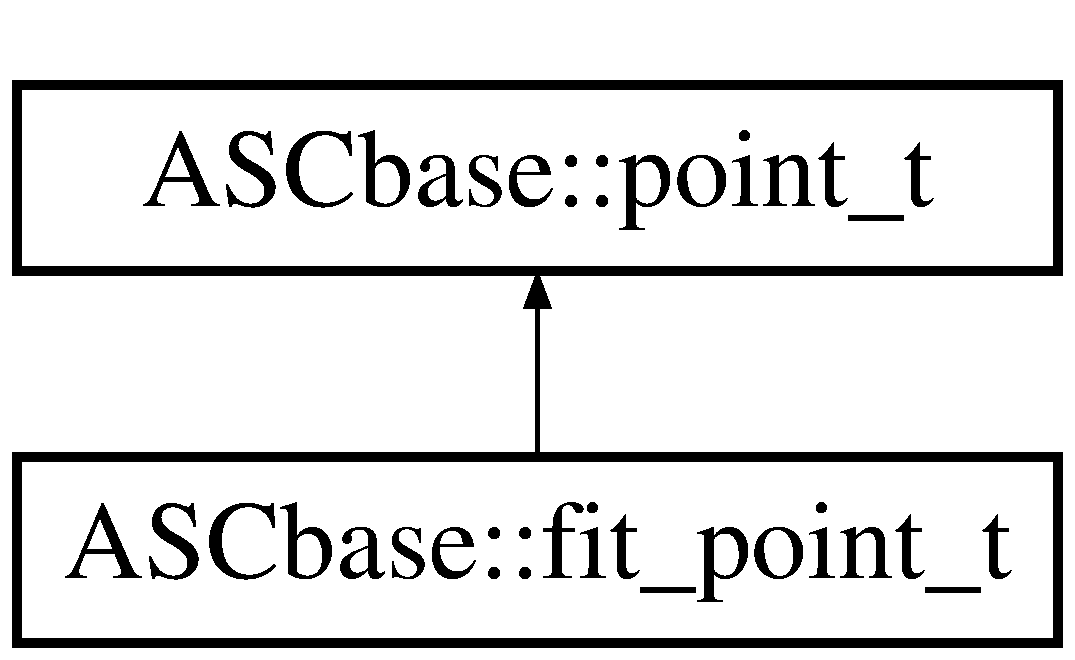
\includegraphics[height=2cm]{classASCbase_1_1fit__point__t}
\end{center}
\end{figure}
\subsection*{Public Member Functions}
\begin{CompactItemize}
\item 
\bf{fit\_\-point\_\-t} (alloc\_\-t a=ALLOC\_\-POSITION)\label{classASCbase_1_1fit__point__t_dd761e7b147a311e47e84e607e5848f3}

\begin{CompactList}\small\item\em Basic cstr -- calls point\_\-t::cstr to handle the position. \item\end{CompactList}\item 
\bf{fit\_\-point\_\-t} (const \bf{fit\_\-point\_\-t} \&p)
\item 
const \bf{fit\_\-point\_\-t} \& \textbf{operator=} (const \bf{fit\_\-point\_\-t} \&p)\label{classASCbase_1_1fit__point__t_b088b51a4fde7e6060bde3da9b7bd95b}

\end{CompactItemize}
\subsection*{Private Member Functions}
\begin{CompactItemize}
\item 
void \textbf{do\_\-copy} (const \bf{fit\_\-point\_\-t} \&p)\label{classASCbase_1_1fit__point__t_0d527c27c49c4e4290948aed8b40ac7f}

\end{CompactItemize}
\subsection*{Private Attributes}
\begin{CompactItemize}
\item 
interaction\-Type \bf{act\_\-type}\label{classASCbase_1_1fit__point__t_63623ba84e89eba6f1712251f7f099ce}

\begin{CompactList}\small\item\em Acceptor, Donor or Hydrophobic. \item\end{CompactList}\item 
std::vector$<$ atom\_\-vci $>$ \bf{atoms}\label{classASCbase_1_1fit__point__t_b5d60780b42c7d83a11764010b05dd88}

\begin{CompactList}\small\item\em Atom or atoms making the interaction at this point. \item\end{CompactList}\end{CompactItemize}


\subsection{Detailed Description}
Used to \char`\"{}harbor\char`\"{} the points used to align sitemaps. For now the direction is handled in a separate \char`\"{}array\char`\"{} 



\subsection{Constructor \& Destructor Documentation}
\index{ASCbase::fit_point_t@{ASCbase::fit\_\-point\_\-t}!fit_point_t@{fit\_\-point\_\-t}}
\index{fit_point_t@{fit\_\-point\_\-t}!ASCbase::fit_point_t@{ASCbase::fit\_\-point\_\-t}}
\subsubsection{\setlength{\rightskip}{0pt plus 5cm}ASCbase::fit\_\-point\_\-t::fit\_\-point\_\-t (const \bf{fit\_\-point\_\-t} \& {\em p})\hspace{0.3cm}{\tt  [inline]}}\label{classASCbase_1_1fit__point__t_c316016e3b9987d7130d0ddc6e14ca82}


Basic copy cstr -- required so that we can call the copy cstr for the \doxyref{point\_\-t}{p.}{classASCbase_1_1point__t} class. 

The documentation for this class was generated from the following file:\begin{CompactItemize}
\item 
fit\_\-point\_\-t.H\end{CompactItemize}

\section{ASCbase::Gen\-Points\-Parameters Class Reference}
\label{classASCbase_1_1GenPointsParameters}\index{ASCbase::GenPointsParameters@{ASCbase::GenPointsParameters}}
{\tt \#include $<$Gen\-Points\-Parameters.H$>$}

Inheritance diagram for ASCbase::Gen\-Points\-Parameters::\begin{figure}[H]
\begin{center}
\leavevmode
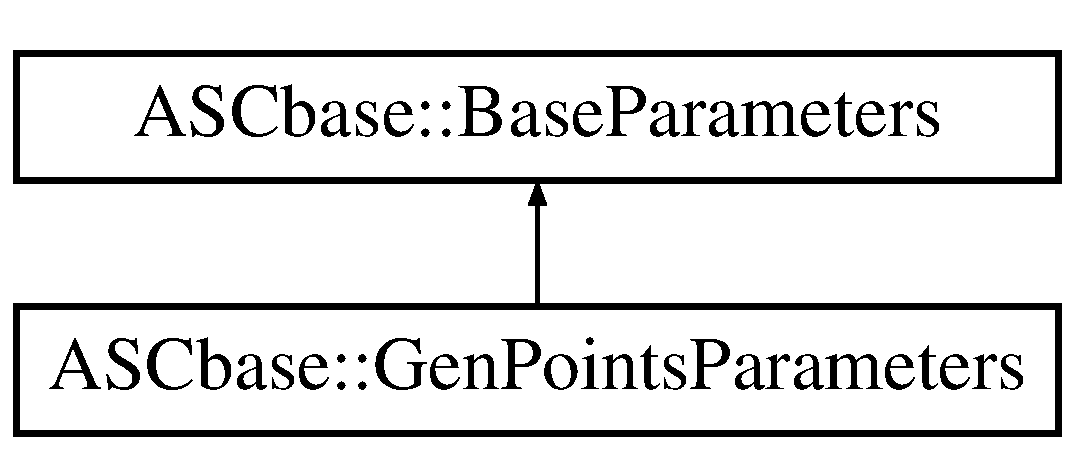
\includegraphics[height=2cm]{classASCbase_1_1GenPointsParameters}
\end{center}
\end{figure}
\subsection*{Public Types}
\begin{CompactItemize}
\item 
\textbf{HBOND\_\-DENSITY\_\-NOT\_\-SET} = 0\label{classASCbase_1_1GenPointsParameters_a6dc6c525bc5758a44eb9713cefd1723e688eab2cad3af9d2259c058a16d5b56}

\item 
\textbf{OPTIMUM\_\-HBONDS}\label{classASCbase_1_1GenPointsParameters_a6dc6c525bc5758a44eb9713cefd17235d922243dad4c74f5bb3ee51b4fa9cca}

\item 
\textbf{MIN\_\-HBONDS}\label{classASCbase_1_1GenPointsParameters_a6dc6c525bc5758a44eb9713cefd172334567d4374013484f1c5292e35476923}

\item 
\textbf{SPARSE\_\-HBONDS}\label{classASCbase_1_1GenPointsParameters_a6dc6c525bc5758a44eb9713cefd172304e35e28876cc1a0b8233d59289eb77e}

\item 
\textbf{DENSE\_\-HBONDS}\label{classASCbase_1_1GenPointsParameters_a6dc6c525bc5758a44eb9713cefd17230f73dadf3a647e598663425e6e951160}

\item 
\textbf{HPHOB\_\-METHOD\_\-NOT\_\-SET}\label{classASCbase_1_1GenPointsParameters_669b793f08bf6d29c9ad36ec0b86dc8727b8532e6c6beb509c7427f833133ed7}

\item 
\bf{THREE\_\-PROTEIN\_\-ATOMS}
\begin{CompactList}\small\item\em If 3+ atoms are close ==$>$ hphob pt. \item\end{CompactList}\item 
\bf{THREE\_\-MORE\_\-HPHOB}
\begin{CompactList}\small\item\em If 3 more hphob than hphil are close. \item\end{CompactList}\item 
\bf{ATOM\_\-CENTERS}
\begin{CompactList}\small\item\em Use centers of Cs and Ses if they have no polar neighbor. \item\end{CompactList}\item 
\textbf{PSEUDO\_\-SURFACE}\label{classASCbase_1_1GenPointsParameters_669b793f08bf6d29c9ad36ec0b86dc87eaa2b64cc234cc13c6f9874d56b372ed}

\item 
\bf{BURIED\_\-SURFACE\_\-AREA}
\begin{CompactList}\small\item\em not implemented yet. \item\end{CompactList}\item 
\textbf{POPT\_\-NULL\_\-FLAG} = 0\label{classASCbase_1_1GenPointsParameters_faf3f5a36bde14fcc55216a5a441d22c507ec8a5e3369d62c1ec200e2335b30e}

\item 
\textbf{DISPLAY\_\-VERSION}\label{classASCbase_1_1GenPointsParameters_faf3f5a36bde14fcc55216a5a441d22cac25ab71c5790952b95202c275440bf3}

\item 
\textbf{NO\_\-NORMALIZATION}\label{classASCbase_1_1GenPointsParameters_faf3f5a36bde14fcc55216a5a441d22cee2409cc901b27f64edaf27996773f72}

\item 
\textbf{BASELINE\_\-HPHOB\_\-REP}\label{classASCbase_1_1GenPointsParameters_faf3f5a36bde14fcc55216a5a441d22cd47a15d3e041c7bec7ad4062987cce7b}

\item 
\textbf{PSEUDO\_\-SURF\_\-HPHOB\_\-REP}\label{classASCbase_1_1GenPointsParameters_faf3f5a36bde14fcc55216a5a441d22c8022c679f6f2f4d07df7b8167b0553a0}

\item 
\textbf{MSMS\_\-SURFACE}\label{classASCbase_1_1GenPointsParameters_faf3f5a36bde14fcc55216a5a441d22cb6df0d8c92eb69322012019cd4c7e6bc}

\item 
\textbf{INCLUDE\_\-WATERS}\label{classASCbase_1_1GenPointsParameters_faf3f5a36bde14fcc55216a5a441d22ce1f56066e8c7b659cb87e8133fce088e}

\item 
\textbf{INCLUDE\_\-METALS}\label{classASCbase_1_1GenPointsParameters_faf3f5a36bde14fcc55216a5a441d22c1eee5307aab4b23b7a8c55ec64879d65}

\item 
\textbf{ALLOW\_\-SMALL\_\-SITEMAPS}\label{classASCbase_1_1GenPointsParameters_faf3f5a36bde14fcc55216a5a441d22c62ed09d823d8e862ab3b381db5dec8cd}

\item 
\textbf{USE\_\-BOUNDING\_\-BOX\_\-FOR\_\-SITE\_\-VOLUME}\label{classASCbase_1_1GenPointsParameters_faf3f5a36bde14fcc55216a5a441d22ccc3dd9740cf50c84fc06351aed0a7efc}

\item 
enum \bf{hbond\_\-method\_\-t} \{ \par
\textbf{HBOND\_\-DENSITY\_\-NOT\_\-SET} =  0, 
\textbf{OPTIMUM\_\-HBONDS}, 
\textbf{MIN\_\-HBONDS}, 
\textbf{SPARSE\_\-HBONDS}, 
\par
\textbf{DENSE\_\-HBONDS}
 \}
\begin{CompactList}\small\item\em Density at which to place hbonds. \item\end{CompactList}\item 
enum \bf{hphob\_\-method\_\-t} \{ \par
\textbf{HPHOB\_\-METHOD\_\-NOT\_\-SET}, 
\bf{THREE\_\-PROTEIN\_\-ATOMS}, 
\bf{THREE\_\-MORE\_\-HPHOB}, 
\bf{ATOM\_\-CENTERS}, 
\par
\textbf{PSEUDO\_\-SURFACE}, 
\bf{BURIED\_\-SURFACE\_\-AREA}
 \}
\item 
enum \textbf{popt\_\-flag\_\-t} \{ \par
\textbf{POPT\_\-NULL\_\-FLAG} =  0, 
\textbf{DISPLAY\_\-VERSION}, 
\textbf{NO\_\-NORMALIZATION}, 
\textbf{BASELINE\_\-HPHOB\_\-REP}, 
\par
\textbf{PSEUDO\_\-SURF\_\-HPHOB\_\-REP}, 
\textbf{MSMS\_\-SURFACE}, 
\textbf{INCLUDE\_\-WATERS}, 
\textbf{INCLUDE\_\-METALS}, 
\par
\textbf{ALLOW\_\-SMALL\_\-SITEMAPS}, 
\textbf{USE\_\-BOUNDING\_\-BOX\_\-FOR\_\-SITE\_\-VOLUME}
 \}
\end{CompactItemize}
\subsection*{Public Member Functions}
\begin{CompactItemize}
\item 
\bf{Gen\-Points\-Parameters} ()\label{classASCbase_1_1GenPointsParameters_a426cd5d7c5ac3ab2663926dd53eb3ca}

\begin{CompactList}\small\item\em To be used by the ASCbase\-Py search.parameters module. \item\end{CompactList}\item 
\textbf{Gen\-Points\-Parameters} (const int argc, const char $\ast$$\ast$argv)\label{classASCbase_1_1GenPointsParameters_5b8d65aa1c03512373ded11690124e39}

\item 
status\_\-t \bf{verify\_\-params} ()
\begin{CompactList}\small\item\em Simple verification of command line parameters. \item\end{CompactList}\end{CompactItemize}
\subsection*{Public Attributes}
\begin{CompactItemize}
\item 
std::string \bf{pts\_\-fname}\label{classASCbase_1_1GenPointsParameters_79dd8921a954695422538728d6639237}

\begin{CompactList}\small\item\em Path to sitemap points file. \item\end{CompactList}\item 
std::string \bf{prot\_\-fname}\label{classASCbase_1_1GenPointsParameters_05078c8d1e24090b73fd7c369333f7b6}

\begin{CompactList}\small\item\em Path to the protein file used to build sitemap. \item\end{CompactList}\item 
std::string \bf{lig\_\-fname}\label{classASCbase_1_1GenPointsParameters_ac65336267172c8cd6ca48460ee0d5c1}

\begin{CompactList}\small\item\em Path to the ligand file used to build sitemap. \item\end{CompactList}\item 
std::string \bf{sphere\_\-str}\label{classASCbase_1_1GenPointsParameters_02d0ab1389a94e6af95bfd41e7c29886}

\begin{CompactList}\small\item\em center and radius of sphere for bind vol \item\end{CompactList}\item 
std::string \textbf{msms\_\-binary}\label{classASCbase_1_1GenPointsParameters_95bed3fd5d293c812cd94e3b2897403c}

\item 
my\_\-float\_\-t \textbf{cluster\_\-diameter}\label{classASCbase_1_1GenPointsParameters_21db5f929abf2e6d96b0882348e4409c}

\item 
my\_\-float\_\-t \textbf{grid\_\-spacing}\label{classASCbase_1_1GenPointsParameters_c98bc4c883738a6a6a1326cb558309d6}

\item 
\bf{hbond\_\-method\_\-t} \textbf{hbond\_\-method}\label{classASCbase_1_1GenPointsParameters_de38ca2fd33a6acbe0e87dfc35e80bd6}

\item 
\bf{hphob\_\-method\_\-t} \textbf{hphob\_\-method}\label{classASCbase_1_1GenPointsParameters_fdd910cc8547b6d8d3002fc28a66ac55}

\item 
sphere\_\-sample\_\-level\_\-t \textbf{sphere\_\-sample\_\-level}\label{classASCbase_1_1GenPointsParameters_5179c24f094735ab2acc005db4883bf5}

\item 
bool \bf{normalize}\label{classASCbase_1_1GenPointsParameters_983e1f910e4ebaeb9643321de06daa35}

\begin{CompactList}\small\item\em True imples normalize sitemap score against diverse set. \item\end{CompactList}\item 
bool \bf{include\_\-metals}\label{classASCbase_1_1GenPointsParameters_91368798e51ab6ee01cf3f7c9a64f823}

\begin{CompactList}\small\item\em True imples include metals in protein file as part of the protein, otherwise ignore all metal atoms. \item\end{CompactList}\item 
std::vector$<$ std::string $>$ \bf{waters}\label{classASCbase_1_1GenPointsParameters_f511959ee5a34fff689e91dab5fb6107}

\begin{CompactList}\small\item\em Water residues to include. \item\end{CompactList}\item 
verbose\_\-level\_\-t \textbf{verbose\_\-level}\label{classASCbase_1_1GenPointsParameters_23b94685b55610bf965937ff9526d2f7}

\item 
bool \bf{call\_\-msms}\label{classASCbase_1_1GenPointsParameters_d51ad728c58114a8b15191fd71cbb3bb}

\begin{CompactList}\small\item\em True implies call \$ASCBASE\_\-INSTALL\_\-DIR/bin/linux\_\-msms to create the site's surface. \item\end{CompactList}\item 
bool \bf{prune\_\-to\_\-lig}\label{classASCbase_1_1GenPointsParameters_c19531d3b882b413a716f26c221c948a}

\begin{CompactList}\small\item\em True implies use the \doxyref{Union\-Of\-Balls}{p.}{classASCbase_1_1UnionOfBalls} class rather than the \doxyref{Rectangular\-Solid}{p.}{classASCbase_1_1RectangularSolid} class for site map volume defined by ligand. \item\end{CompactList}\item 
my\_\-float\_\-t \bf{probe\_\-radius}\label{classASCbase_1_1GenPointsParameters_58e2eba3c8127ca6727c816fc25fbc0b}

\begin{CompactList}\small\item\em Probe radius for MSMS. \item\end{CompactList}\item 
my\_\-float\_\-t \bf{num\_\-pts\_\-per\_\-area}\label{classASCbase_1_1GenPointsParameters_72c2161d8a4f040c834a00b2a6d4b65f}

\begin{CompactList}\small\item\em Number of points per (A)$^\wedge$2. \item\end{CompactList}\item 
std::string \bf{user\_\-provided\_\-surf}\label{classASCbase_1_1GenPointsParameters_a937ce73cf3d435fc709d237afcbb1d7}

\begin{CompactList}\small\item\em Path to user provided msms\_\-surf.vert file -- assumes a corresponding msms\_\-surf.face file. \item\end{CompactList}\item 
int \bf{min\_\-res\_\-per\_\-chain}\label{classASCbase_1_1GenPointsParameters_36834569dd27d585271d5e6e692e543e}

\begin{CompactList}\small\item\em Minimum number of residues per chain. \item\end{CompactList}\end{CompactItemize}
\subsection*{Private Member Functions}
\begin{CompactItemize}
\item 
void \bf{init} ()
\item 
void \bf{free\_\-cstrings} ()\label{classASCbase_1_1GenPointsParameters_60f2e20d62c182976441ce8033ffcd8b}

\begin{CompactList}\small\item\em Free up all C-style strings which are not NULL; calls \doxyref{init()}{p.}{classASCbase_1_1GenPointsParameters_4f832e2354ce25bfdc4d2328ea1fdbb3} at the end. \item\end{CompactList}\item 
status\_\-t \bf{get\_\-opts} (const int argc, const char $\ast$$\ast$argv)
\begin{CompactList}\small\item\em Given the command line arguments, parse them using the popt library. \item\end{CompactList}\end{CompactItemize}
\subsection*{Private Attributes}
\begin{CompactItemize}
\item 
char $\ast$ \bf{prots\_\-dir}\label{classASCbase_1_1GenPointsParameters_20837ede82f1e0354e32379f31b1eb7e}

\begin{CompactList}\small\item\em Cmdline value for \$ASCBASE\_\-DBASE\_\-PROTS. \item\end{CompactList}\item 
char $\ast$ \bf{ligs\_\-dir}\label{classASCbase_1_1GenPointsParameters_0ce67d820a04b3f1b66cb1a2e20f2b1a}

\begin{CompactList}\small\item\em Cmdline value for \$ASCBASE\_\-DBASE\_\-LIGS. \item\end{CompactList}\item 
char $\ast$ \bf{hbond\_\-dens\_\-str}\label{classASCbase_1_1GenPointsParameters_71019cf273be68799c0aaf1a4810ebda}

\begin{CompactList}\small\item\em Cmdline value for hydrogen bond density. \item\end{CompactList}\item 
char $\ast$ \bf{A\_\-scratch\_\-dir}\label{classASCbase_1_1GenPointsParameters_92c9bf42be518371aa1ab5dab5e2ecd6}

\begin{CompactList}\small\item\em Cmdline value for \$ASCBASE\_\-SCRATCH\_\-DIR. \item\end{CompactList}\item 
char $\ast$ \bf{A\_\-proj\_\-output}\label{classASCbase_1_1GenPointsParameters_d1350f739351e459cab5873b64495eb7}

\begin{CompactList}\small\item\em Cmdline value for \$ASCBASE\_\-PROJ\_\-OUTPUT. \item\end{CompactList}\item 
char $\ast$ \bf{A\_\-waters\_\-str}\label{classASCbase_1_1GenPointsParameters_45d697045acd2449ad1780736a370d41}

\begin{CompactList}\small\item\em Cmdline string for water residues to include. \item\end{CompactList}\end{CompactItemize}
\subsection*{Static Private Attributes}
\begin{CompactItemize}
\item 
static const std::string \bf{A\_\-fname} = \char`\"{}Gen\-Points\-Parameters.C\char`\"{}\label{classASCbase_1_1GenPointsParameters_be5f9a9a270525cabb91c7b7058a873b}

\begin{CompactList}\small\item\em Name of source file. \item\end{CompactList}\end{CompactItemize}


\subsection{Detailed Description}
Unlike the base class, the string parameters here are all cstrings to support the popt library for parsing command line options 



\subsection{Member Enumeration Documentation}
\index{ASCbase::GenPointsParameters@{ASCbase::Gen\-Points\-Parameters}!hphob_method_t@{hphob\_\-method\_\-t}}
\index{hphob_method_t@{hphob\_\-method\_\-t}!ASCbase::GenPointsParameters@{ASCbase::Gen\-Points\-Parameters}}
\subsubsection{\setlength{\rightskip}{0pt plus 5cm}enum \bf{ASCbase::Gen\-Points\-Parameters::hphob\_\-method\_\-t}}\label{classASCbase_1_1GenPointsParameters_669b793f08bf6d29c9ad36ec0b86dc87}


\begin{Desc}
\item[Enumerator: ]\par
\begin{description}
\index{THREE_PROTEIN_ATOMS@{THREE\_\-PROTEIN\_\-ATOMS}!ASCbase::GenPointsParameters@{ASCbase::GenPointsParameters}}\index{ASCbase::GenPointsParameters@{ASCbase::GenPointsParameters}!THREE_PROTEIN_ATOMS@{THREE\_\-PROTEIN\_\-ATOMS}}\item[{\em 
THREE\_\-PROTEIN\_\-ATOMS\label{classASCbase_1_1GenPointsParameters_669b793f08bf6d29c9ad36ec0b86dc879251dffd62e1337ccdb51478be13a351}
}]If 3+ atoms are close ==$>$ hphob pt. \index{THREE_MORE_HPHOB@{THREE\_\-MORE\_\-HPHOB}!ASCbase::GenPointsParameters@{ASCbase::GenPointsParameters}}\index{ASCbase::GenPointsParameters@{ASCbase::GenPointsParameters}!THREE_MORE_HPHOB@{THREE\_\-MORE\_\-HPHOB}}\item[{\em 
THREE\_\-MORE\_\-HPHOB\label{classASCbase_1_1GenPointsParameters_669b793f08bf6d29c9ad36ec0b86dc8785898d66a04a45a72e894e1609c75fe6}
}]If 3 more hphob than hphil are close. \index{ATOM_CENTERS@{ATOM\_\-CENTERS}!ASCbase::GenPointsParameters@{ASCbase::GenPointsParameters}}\index{ASCbase::GenPointsParameters@{ASCbase::GenPointsParameters}!ATOM_CENTERS@{ATOM\_\-CENTERS}}\item[{\em 
ATOM\_\-CENTERS\label{classASCbase_1_1GenPointsParameters_669b793f08bf6d29c9ad36ec0b86dc87f711be0650735616b19365c4865e9d55}
}]Use centers of Cs and Ses if they have no polar neighbor. \index{BURIED_SURFACE_AREA@{BURIED\_\-SURFACE\_\-AREA}!ASCbase::GenPointsParameters@{ASCbase::GenPointsParameters}}\index{ASCbase::GenPointsParameters@{ASCbase::GenPointsParameters}!BURIED_SURFACE_AREA@{BURIED\_\-SURFACE\_\-AREA}}\item[{\em 
BURIED\_\-SURFACE\_\-AREA\label{classASCbase_1_1GenPointsParameters_669b793f08bf6d29c9ad36ec0b86dc8700da31656ba41bd2040e09c8f0b7070b}
}]not implemented yet. \end{description}
\end{Desc}



\subsection{Member Function Documentation}
\index{ASCbase::GenPointsParameters@{ASCbase::Gen\-Points\-Parameters}!get_opts@{get\_\-opts}}
\index{get_opts@{get\_\-opts}!ASCbase::GenPointsParameters@{ASCbase::Gen\-Points\-Parameters}}
\subsubsection{\setlength{\rightskip}{0pt plus 5cm}Base\-Parameters::status\_\-t Gen\-Points\-Parameters::get\_\-opts (const int {\em argc}, const char $\ast$$\ast$ {\em argv})\hspace{0.3cm}{\tt  [private]}}\label{classASCbase_1_1GenPointsParameters_edbe9849101dc338a5fe1666f654775f}


Given the command line arguments, parse them using the popt library. 

\begin{Desc}
\item[Parameters:]
\begin{description}
\item[{\em argc}]Number of command line arguments \item[{\em argv}]Array of C-style strings holding the command line arguments \end{description}
\end{Desc}
\begin{Desc}
\item[Returns:]True if parsed successfully and may continue, else false \end{Desc}
\index{ASCbase::GenPointsParameters@{ASCbase::Gen\-Points\-Parameters}!init@{init}}
\index{init@{init}!ASCbase::GenPointsParameters@{ASCbase::Gen\-Points\-Parameters}}
\subsubsection{\setlength{\rightskip}{0pt plus 5cm}void Gen\-Points\-Parameters::init ()\hspace{0.3cm}{\tt  [private]}}\label{classASCbase_1_1GenPointsParameters_4f832e2354ce25bfdc4d2328ea1fdbb3}


Initialize the class variables to standard nondefined values (such as NULL). \index{ASCbase::GenPointsParameters@{ASCbase::Gen\-Points\-Parameters}!verify_params@{verify\_\-params}}
\index{verify_params@{verify\_\-params}!ASCbase::GenPointsParameters@{ASCbase::Gen\-Points\-Parameters}}
\subsubsection{\setlength{\rightskip}{0pt plus 5cm}Base\-Parameters::status\_\-t Gen\-Points\-Parameters::verify\_\-params ()}\label{classASCbase_1_1GenPointsParameters_603bc78f168807251675b54eb0d39fa0}


Simple verification of command line parameters. 

Don't think this needs to be private \begin{Desc}
\item[Returns:]False implies unsafe to proceed, otherwise should be OK \end{Desc}


The documentation for this class was generated from the following files:\begin{CompactItemize}
\item 
Gen\-Points\-Parameters.H\item 
Gen\-Points\-Parameters.C\end{CompactItemize}

\section{ASCbase::geometry::half\_\-edge\_\-t Struct Reference}
\label{structASCbase_1_1geometry_1_1half__edge__t}\index{ASCbase::geometry::half_edge_t@{ASCbase::geometry::half\_\-edge\_\-t}}
Simple half edge structure.  


{\tt \#include $<$Tri\-Mesh\-Sphere.H$>$}

\subsection*{Public Attributes}
\begin{CompactItemize}
\item 
std::vector$<$ \bf{half\_\-edge\_\-t} $>$::iterator \textbf{next}\label{structASCbase_1_1geometry_1_1half__edge__t_b9c1024184c488466c7e8f0f155ea959}

\item 
vertex\_\-vci \textbf{tail}\label{structASCbase_1_1geometry_1_1half__edge__t_24e846910bcc790ee9eb33bd0995b336}

\end{CompactItemize}


\subsection{Detailed Description}
Simple half edge structure. 



The documentation for this struct was generated from the following file:\begin{CompactItemize}
\item 
Tri\-Mesh\-Sphere.H\end{CompactItemize}

\section{ASCbase::hbond\_\-ideal\_\-point\_\-t Class Reference}
\label{classASCbase_1_1hbond__ideal__point__t}\index{ASCbase::hbond_ideal_point_t@{ASCbase::hbond\_\-ideal\_\-point\_\-t}}
An \char`\"{}ideal\char`\"{} hbond point.  


{\tt \#include $<$hbond\_\-points.H$>$}

Inheritance diagram for ASCbase::hbond\_\-ideal\_\-point\_\-t::\begin{figure}[H]
\begin{center}
\leavevmode
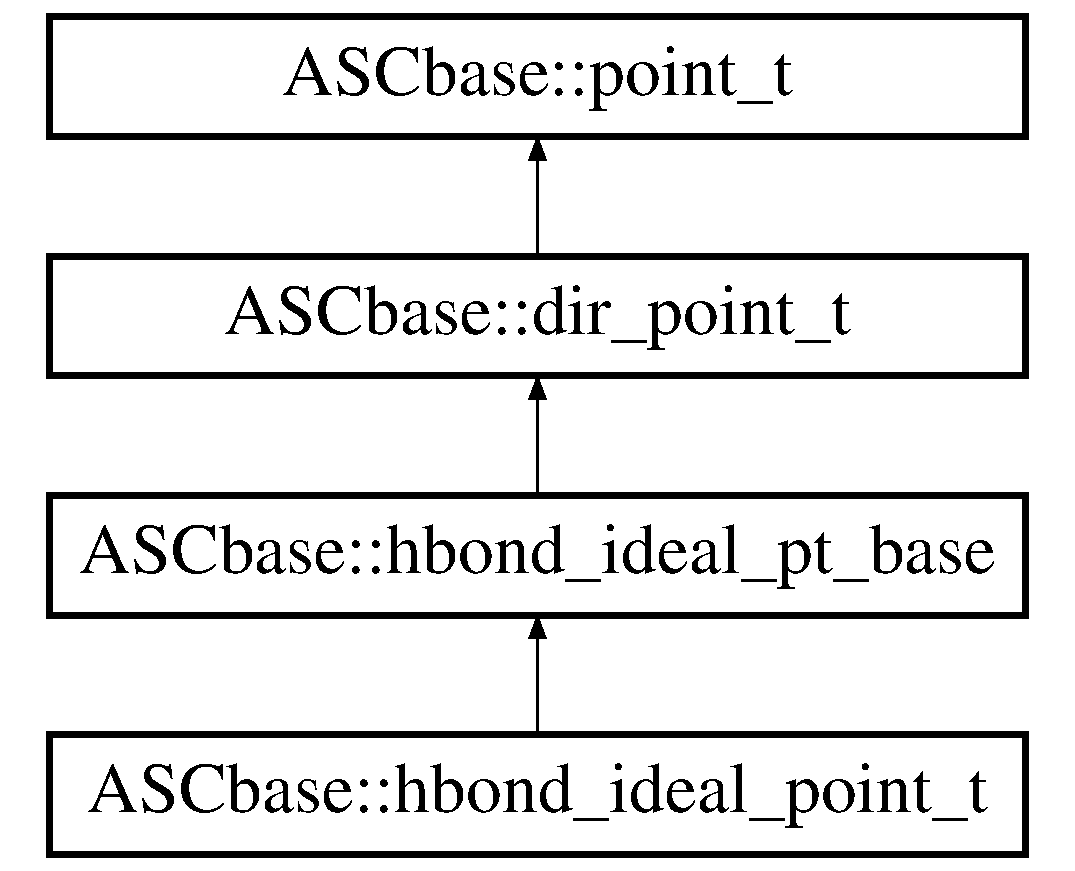
\includegraphics[height=4cm]{classASCbase_1_1hbond__ideal__point__t}
\end{center}
\end{figure}
\subsection*{Public Member Functions}
\begin{CompactItemize}
\item 
\textbf{hbond\_\-ideal\_\-point\_\-t} (alloc\_\-t a=ALLOC\_\-POSITION)\label{classASCbase_1_1hbond__ideal__point__t_17edfda196584b6b9f2bd4c26ada8d7a}

\item 
\textbf{hbond\_\-ideal\_\-point\_\-t} (const \bf{hbond\_\-ideal\_\-point\_\-t} \&p)\label{classASCbase_1_1hbond__ideal__point__t_51934c9d9788021b09d2d24eb5b976e7}

\item 
const \bf{hbond\_\-ideal\_\-point\_\-t} \& \textbf{operator=} (const \bf{hbond\_\-ideal\_\-point\_\-t} \&p)\label{classASCbase_1_1hbond__ideal__point__t_9fcb68e2f672eebb7505ed413123a78c}

\end{CompactItemize}
\subsection*{Public Attributes}
\begin{CompactItemize}
\item 
hbond\_\-fit\_\-pt\_\-vci \bf{fit\_\-pts\_\-beg}\label{classASCbase_1_1hbond__ideal__point__t_620a62e5bfaeb61bc5815745a60aed5c}

\begin{CompactList}\small\item\em Const iter to the first fit point corresponding to this ideal point. \item\end{CompactList}\item 
hbond\_\-fit\_\-pt\_\-vci \bf{fit\_\-pts\_\-end}\label{classASCbase_1_1hbond__ideal__point__t_fd82444a9d7addc28b06b24e9b9badee}

\begin{CompactList}\small\item\em Const iter to 1 past the end of the fit points corresponding to this ideal point. \item\end{CompactList}\end{CompactItemize}
\subsection*{Private Member Functions}
\begin{CompactItemize}
\item 
void \textbf{do\_\-copy} (const \bf{hbond\_\-ideal\_\-point\_\-t} \&p)\label{classASCbase_1_1hbond__ideal__point__t_7cc7e353e9bce5777ffdf83cda34778b}

\end{CompactItemize}


\subsection{Detailed Description}
An \char`\"{}ideal\char`\"{} hbond point. 



The documentation for this class was generated from the following file:\begin{CompactItemize}
\item 
hbond\_\-points.H\end{CompactItemize}

\section{ASCbase::hbond\_\-ideal\_\-pt\_\-base Class Reference}
\label{classASCbase_1_1hbond__ideal__pt__base}\index{ASCbase::hbond_ideal_pt_base@{ASCbase::hbond\_\-ideal\_\-pt\_\-base}}
An \char`\"{}ideal\char`\"{} hbond point base class.  


{\tt \#include $<$hbond\_\-points.H$>$}

Inheritance diagram for ASCbase::hbond\_\-ideal\_\-pt\_\-base::\begin{figure}[H]
\begin{center}
\leavevmode
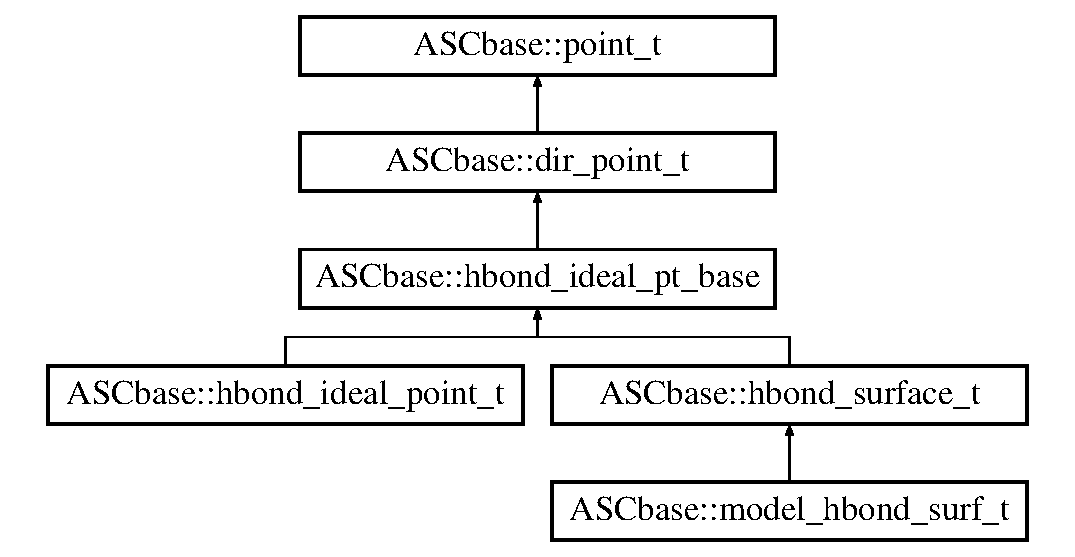
\includegraphics[height=5cm]{classASCbase_1_1hbond__ideal__pt__base}
\end{center}
\end{figure}
\subsection*{Public Member Functions}
\begin{CompactItemize}
\item 
\textbf{hbond\_\-ideal\_\-pt\_\-base} (alloc\_\-t a=ALLOC\_\-POSITION)\label{classASCbase_1_1hbond__ideal__pt__base_6c727a2312275eeca47a7a36b27ff531}

\item 
\textbf{hbond\_\-ideal\_\-pt\_\-base} (const atom\_\-vci hbond\_\-atom, const atom\_\-vci C\_\-nbr\_\-atom, const atom\_\-vci second\_\-nbr\_\-atom, const \bf{Bounding\-Volume} \&site\_\-vol, const int cap\_\-number, const bool include\_\-metals=false, const alloc\_\-t a=ALLOC\_\-POSITION)\label{classASCbase_1_1hbond__ideal__pt__base_8c6aebede051225c5d7732dff3c9de61}

\item 
\textbf{hbond\_\-ideal\_\-pt\_\-base} (const \bf{hbond\_\-ideal\_\-pt\_\-base} \&p)\label{classASCbase_1_1hbond__ideal__pt__base_6b1afae556e880d14099bdca58304d46}

\item 
const \bf{hbond\_\-ideal\_\-pt\_\-base} \& \textbf{operator=} (const \bf{hbond\_\-ideal\_\-pt\_\-base} \&p)\label{classASCbase_1_1hbond__ideal__pt__base_a8a595d97addfd2dc71a74230a022dec}

\item 
const \bf{ASCbase::atom\_\-t} \& \textbf{\_\-\_\-get\_\-atom} () const \label{classASCbase_1_1hbond__ideal__pt__base_4ad13839630fecd1c9d561e081b7b18e}

\item 
const \bf{ASCbase::atom\_\-t} \& \textbf{\_\-\_\-get\_\-carbon\_\-nbr} () const \label{classASCbase_1_1hbond__ideal__pt__base_1e47efb94434d32735034ade4ee4a7fe}

\end{CompactItemize}
\subsection*{Static Public Member Functions}
\begin{CompactItemize}
\item 
static bool \textbf{cmp} (const \bf{hbond\_\-ideal\_\-pt\_\-base} \&A, const \bf{hbond\_\-ideal\_\-pt\_\-base} \&B)\label{classASCbase_1_1hbond__ideal__pt__base_6d6b4ad446addecc3079229713313731}

\end{CompactItemize}
\subsection*{Public Attributes}
\begin{CompactItemize}
\item 
uint \bf{pt\_\-num}\label{classASCbase_1_1hbond__ideal__pt__base_a6829823658e609726d64d46f05a53c4}

\begin{CompactList}\small\item\em Number given to the ideal point. \item\end{CompactList}\item 
interaction\-Type \bf{act\_\-type}\label{classASCbase_1_1hbond__ideal__pt__base_2b226c040314c92bf0e9d0e647f66897}

\begin{CompactList}\small\item\em Interaction type of the points. \item\end{CompactList}\item 
atom\_\-vci \bf{atom}\label{classASCbase_1_1hbond__ideal__pt__base_c69850f24c46ac0c32143cf6f3ac2c91}

\begin{CompactList}\small\item\em Protein heavy atom giving rise to the points. \item\end{CompactList}\item 
atom\_\-vci \bf{carbon\_\-nbr}\label{classASCbase_1_1hbond__ideal__pt__base_7155ffb9e0c06bc4267fb4ee28b9d212}

\begin{CompactList}\small\item\em Carbon atom used to define the acceptor/donor plane. \item\end{CompactList}\item 
atom\_\-vci \bf{second\_\-nbr}\label{classASCbase_1_1hbond__ideal__pt__base_733afddb617c0b55f4887e963d954848}

\begin{CompactList}\small\item\em Third atom used to define the plane. \item\end{CompactList}\end{CompactItemize}
\subsection*{Private Member Functions}
\begin{CompactItemize}
\item 
void \textbf{do\_\-copy} (const \bf{hbond\_\-ideal\_\-pt\_\-base} \&p)\label{classASCbase_1_1hbond__ideal__pt__base_ea14650cc4989d996bb228f2d68e2cee}

\end{CompactItemize}


\subsection{Detailed Description}
An \char`\"{}ideal\char`\"{} hbond point base class. 



The documentation for this class was generated from the following file:\begin{CompactItemize}
\item 
hbond\_\-points.H\end{CompactItemize}

\section{ASCbase::hbond\_\-point\_\-t Class Reference}
\label{classASCbase_1_1hbond__point__t}\index{ASCbase::hbond_point_t@{ASCbase::hbond\_\-point\_\-t}}
A \char`\"{}fit\char`\"{} hbonding point.  


{\tt \#include $<$hbond\_\-points.H$>$}

Inheritance diagram for ASCbase::hbond\_\-point\_\-t::\begin{figure}[H]
\begin{center}
\leavevmode
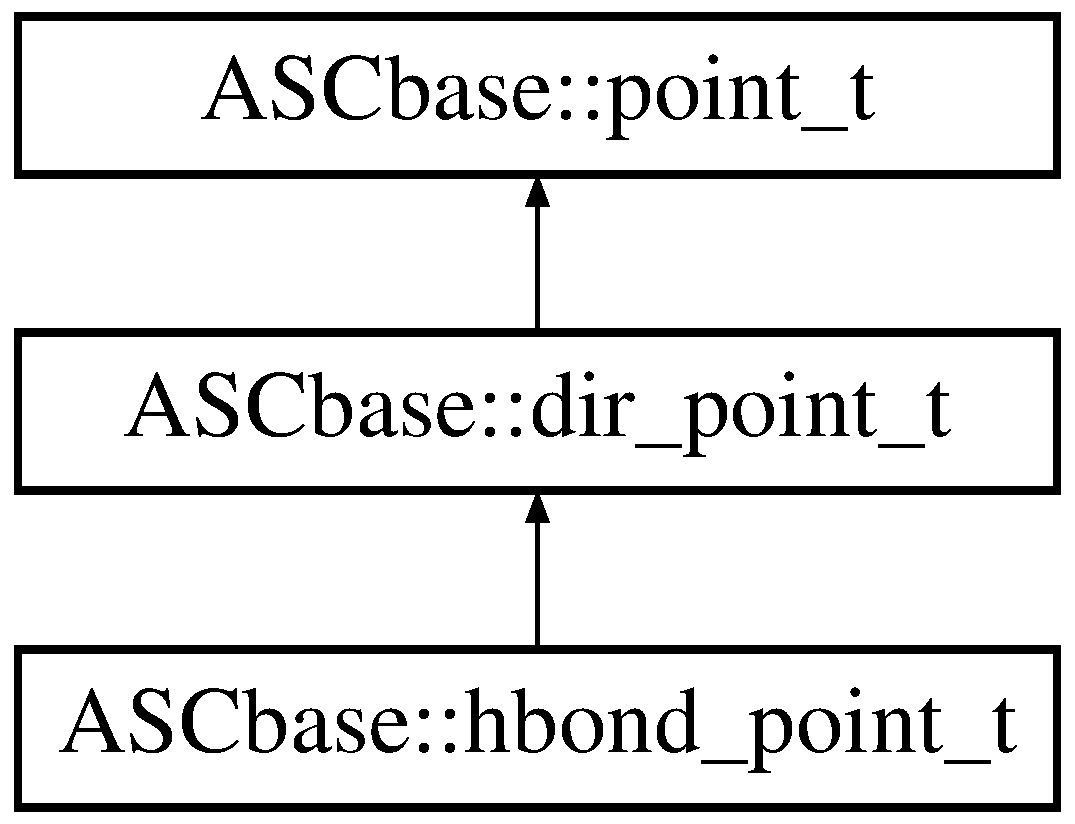
\includegraphics[height=3cm]{classASCbase_1_1hbond__point__t}
\end{center}
\end{figure}
\subsection*{Public Member Functions}
\begin{CompactItemize}
\item 
\textbf{hbond\_\-point\_\-t} (alloc\_\-t a=ALLOC\_\-POSITION)\label{classASCbase_1_1hbond__point__t_5fab75a5579f51c63612ddb147c3eb0a}

\item 
\textbf{hbond\_\-point\_\-t} (const \bf{hbond\_\-point\_\-t} \&p)\label{classASCbase_1_1hbond__point__t_a0e83b45350073eb28ceefc0c995861c}

\item 
const \bf{hbond\_\-point\_\-t} \& \textbf{operator=} (const \bf{hbond\_\-point\_\-t} \&p)\label{classASCbase_1_1hbond__point__t_c77fa3dc05e58c6cede53e560f663291}

\item 
const \bf{ASCbase::atom\_\-t} \& \textbf{\_\-\_\-get\_\-atom} () const \label{classASCbase_1_1hbond__point__t_faf40b7877ec78b4a2e134369fb5e8cf}

\item 
const \bf{ASCbase::hbond\_\-ideal\_\-point\_\-t} \& \textbf{\_\-\_\-get\_\-ideal\_\-pt} () const \label{classASCbase_1_1hbond__point__t_ed40f565437b493c187f56297417d2ec}

\end{CompactItemize}
\subsection*{Static Public Member Functions}
\begin{CompactItemize}
\item 
static bool \textbf{cmp} (const \bf{hbond\_\-point\_\-t} \&A, const \bf{hbond\_\-point\_\-t} \&B)\label{classASCbase_1_1hbond__point__t_86692805c3b0ded25d5e64a74fb8089f}

\end{CompactItemize}
\subsection*{Public Attributes}
\begin{CompactItemize}
\item 
interaction\-Type \bf{act\_\-type}\label{classASCbase_1_1hbond__point__t_64018d64558cbf939525efb893679809}

\begin{CompactList}\small\item\em Interaction type of the points. \item\end{CompactList}\item 
hbond\_\-ideal\_\-pt\_\-vci \bf{ideal\_\-pt}\label{classASCbase_1_1hbond__point__t_9ba48d24b24579d4e3a810af1fc57453}

\begin{CompactList}\small\item\em Iterator to the associated ideal point. \item\end{CompactList}\item 
atom\_\-vci \bf{atom}\label{classASCbase_1_1hbond__point__t_efd938fefea14539848e466c7f08d325}

\begin{CompactList}\small\item\em Heavy atom giving rise to the points. \item\end{CompactList}\end{CompactItemize}
\subsection*{Private Member Functions}
\begin{CompactItemize}
\item 
void \textbf{do\_\-copy} (const \bf{hbond\_\-point\_\-t} \&p)\label{classASCbase_1_1hbond__point__t_ac9aceb4f7f609deebb437ec14b8b15a}

\end{CompactItemize}


\subsection{Detailed Description}
A \char`\"{}fit\char`\"{} hbonding point. 



The documentation for this class was generated from the following file:\begin{CompactItemize}
\item 
hbond\_\-points.H\end{CompactItemize}

\section{ASCbase::hbond\_\-surface\_\-t Class Reference}
\label{classASCbase_1_1hbond__surface__t}\index{ASCbase::hbond_surface_t@{ASCbase::hbond\_\-surface\_\-t}}
{\tt \#include $<$Hbond\-Surfaces.H$>$}

Inheritance diagram for ASCbase::hbond\_\-surface\_\-t::\begin{figure}[H]
\begin{center}
\leavevmode
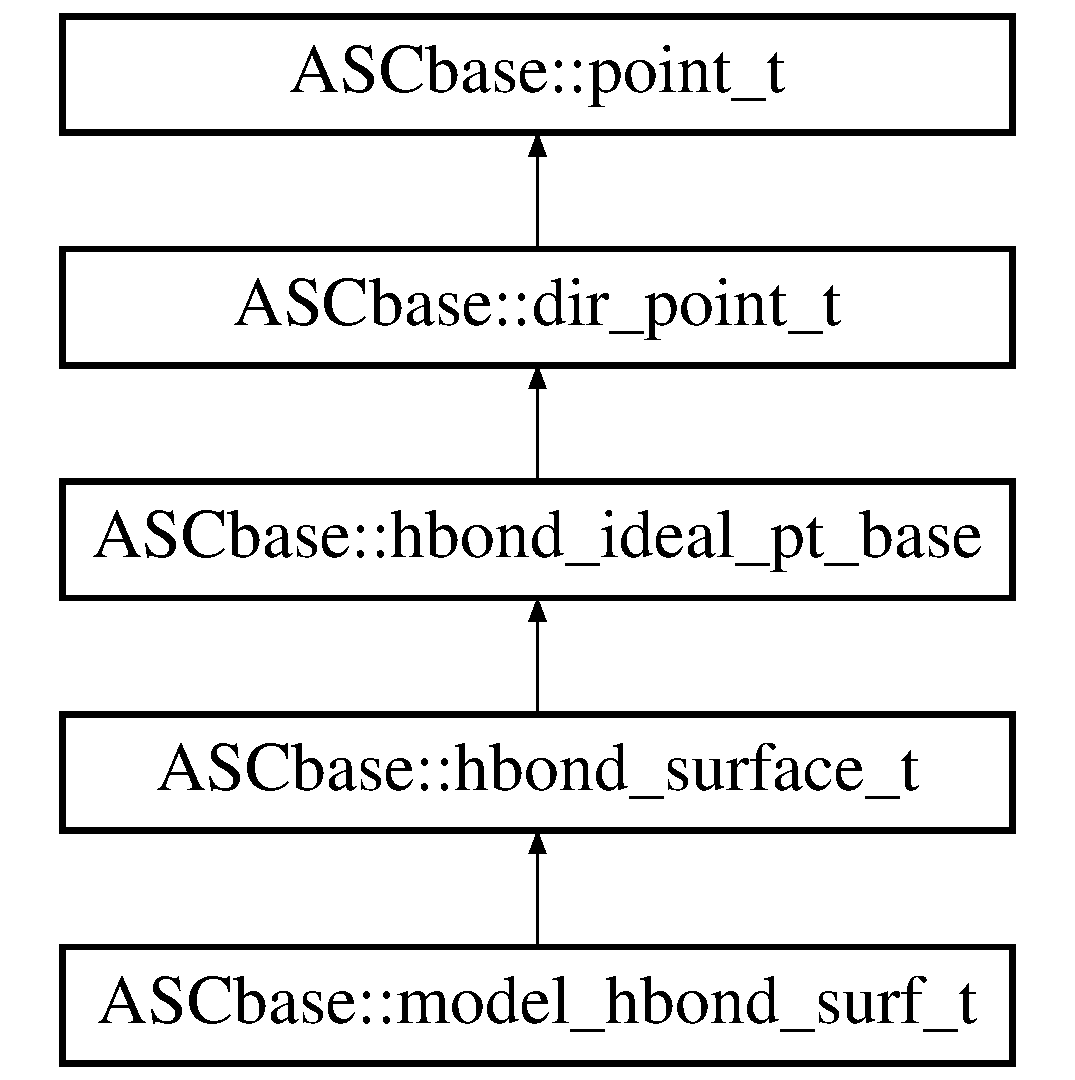
\includegraphics[height=5cm]{classASCbase_1_1hbond__surface__t}
\end{center}
\end{figure}
\subsection*{Public Member Functions}
\begin{CompactItemize}
\item 
\bf{hbond\_\-surface\_\-t} (const atom\_\-vci hbond\_\-atom, const atom\_\-vci C\_\-nbr\_\-atom, const atom\_\-vci second\_\-nbr\_\-atom, \bf{Bounding\-Volume} \&site\_\-vol, const int cap\_\-number, const bool include\_\-metals=false, const alloc\_\-t a=ALLOC\_\-POSITION)\label{classASCbase_1_1hbond__surface__t_9e357e26963a25f5d34f8ead0e7154b8}

\begin{CompactList}\small\item\em Constructor to create the representation. \item\end{CompactList}\item 
\bf{hbond\_\-surface\_\-t} (const std::string \&data\_\-line, \bf{PDBBase} \&prot\_\-atoms)\label{classASCbase_1_1hbond__surface__t_a072af1ca67675f348af7ae0f6a9941b}

\begin{CompactList}\small\item\em Constructor for an existing surface (typically read from file). \item\end{CompactList}\item 
\textbf{hbond\_\-surface\_\-t} (const \bf{hbond\_\-surface\_\-t} \&src)\label{classASCbase_1_1hbond__surface__t_e1e229896cc8285447726191d4c8e5c2}

\item 
const \bf{hbond\_\-surface\_\-t} \& \textbf{operator=} (const \bf{hbond\_\-surface\_\-t} \&src)\label{classASCbase_1_1hbond__surface__t_c825922a0e490482d7f5362d2554beaf}

\item 
bool \textbf{closest\_\-point} (const my\_\-float\_\-t $\ast$pt, my\_\-float\_\-t $\ast$closest\_\-pt, const my\_\-float\_\-t tol=1.0)\label{classASCbase_1_1hbond__surface__t_828b634e714761ec0282112bab50d6f6}

\item 
const my\_\-float\_\-t $\ast$ \textbf{ideal\_\-dir} () const \label{classASCbase_1_1hbond__surface__t_64bcfe8ebae6a5a406fa880eabe4c0b6}

\item 
void \textbf{transform} (const my\_\-float\_\-t $\ast$R, const my\_\-float\_\-t $\ast$T)\label{classASCbase_1_1hbond__surface__t_81063d19a3920c08e846d70928f6c594}

\item 
void \textbf{inverse\_\-transform} (const my\_\-float\_\-t $\ast$R, const my\_\-float\_\-t $\ast$T)\label{classASCbase_1_1hbond__surface__t_203a7593526f7b8d8a20cb664406d6a3}

\item 
void \textbf{revert} ()\label{classASCbase_1_1hbond__surface__t_e65041fc31bbbaae6922364cfe78ae54}

\end{CompactItemize}
\subsection*{Private Member Functions}
\begin{CompactItemize}
\item 
void \textbf{do\_\-copy} (const \bf{hbond\_\-surface\_\-t} \&src)\label{classASCbase_1_1hbond__surface__t_e9299a1f7a8dbf67c3136863dd2df237}

\end{CompactItemize}
\subsection*{Private Attributes}
\begin{CompactItemize}
\item 
geometry::sphere\_\-t \textbf{A\_\-surf}\label{classASCbase_1_1hbond__surface__t_95bfd3372bb83fadd0b1708da01dec8d}

\item 
\bf{geometry::plane\_\-t} \textbf{A\_\-cut\_\-plane}\label{classASCbase_1_1hbond__surface__t_397632033debf716dbcc7fc8ef81fb61}

\item 
my\_\-float\_\-t \bf{A\_\-cap\_\-plane\_\-rad}\label{classASCbase_1_1hbond__surface__t_83046f180c928461d3f67c4b3b81554c}

\begin{CompactList}\small\item\em Radius of cap restricted to cutting plane. \item\end{CompactList}\item 
std::vector$<$ \bf{geometry::i\-Circle} $>$ \textbf{A\_\-circles}\label{classASCbase_1_1hbond__surface__t_f0161567ebb1e37b69510969d76ddb86}

\end{CompactItemize}
\subsection*{Static Private Attributes}
\begin{CompactItemize}
\item 
static const my\_\-float\_\-t \bf{SURF\_\-SPHERE\_\-RAD} = 3.0\label{classASCbase_1_1hbond__surface__t_5779dc1ca7f6d66ef343d01ba14978b8}

\begin{CompactList}\small\item\em Radius of sphere used to define the cap. \item\end{CompactList}\end{CompactItemize}


\subsection{Detailed Description}
I am currently in a bind and to get this working quickly, I am abusing the format to handle metals as well. In the case of metals we do NOT have neighbor atom or an initial cap cutting plane (metals are modeled as not having a prefered direction). However, we do desire to keep the method transformation invariant; to do this we put the closest atom to the metal as the C\_\-nbr\_\-atom and the 2nd closest as the 2nd nbr atom (this is confusing but quick \& dirty). 



The documentation for this class was generated from the following files:\begin{CompactItemize}
\item 
Hbond\-Surfaces.H\item 
Hbond\-Surfaces.C\end{CompactItemize}

\section{ASCbase::hbond\_\-triad\_\-t Struct Reference}
\label{structASCbase_1_1hbond__triad__t}\index{ASCbase::hbond_triad_t@{ASCbase::hbond\_\-triad\_\-t}}
Data struct holding the local ideal hbond position parameters.  


{\tt \#include $<$hbond\_\-triads.H$>$}

\subsection*{Public Attributes}
\begin{CompactItemize}
\item 
residue\_\-type \bf{residue}\label{structASCbase_1_1hbond__triad__t_1798707faec057ecf99c799925405515}

\begin{CompactList}\small\item\em Name of the residue. \item\end{CompactList}\item 
atom\_\-type \bf{nbr\_\-A}\label{structASCbase_1_1hbond__triad__t_c119967e6a52daeb787ee39542b77061}

\begin{CompactList}\small\item\em Name of the first neighbor (carbon nbr). \item\end{CompactList}\item 
atom\_\-type \bf{B}\label{structASCbase_1_1hbond__triad__t_7b75fba196d3ee7c932a6e2ef2f5e731}

\begin{CompactList}\small\item\em Name of the hbond atom. \item\end{CompactList}\item 
atom\_\-type \bf{nbr\_\-C}\label{structASCbase_1_1hbond__triad__t_c130e5b1271da5dde0b3ecceef40ca46}

\begin{CompactList}\small\item\em Name of the second neighbor. \item\end{CompactList}\item 
my\_\-float\_\-t \bf{bond\_\-len}\label{structASCbase_1_1hbond__triad__t_698e8f7f8227cabe2b32be68600d7ae4}

\begin{CompactList}\small\item\em \char`\"{}Average\char`\"{} hbond length (D-A distance) \item\end{CompactList}\item 
interaction\-Type \bf{type}\label{structASCbase_1_1hbond__triad__t_9211af10c6925f80ac7e6a1cb01f92a6}

\begin{CompactList}\small\item\em interaction type to satisify the hbond atom \item\end{CompactList}\item 
int \bf{pt\_\-num}\label{structASCbase_1_1hbond__triad__t_19531534552566a3002c718ccfeef088}

\begin{CompactList}\small\item\em Object number for the hbond atom. \item\end{CompactList}\item 
my\_\-float\_\-t \bf{alpha}\label{structASCbase_1_1hbond__triad__t_b80b511a9b9ed06e7f4ad429e4741aa2}

\begin{CompactList}\small\item\em \char`\"{}In-plane\char`\"{} angle (rotation about Z axis) \item\end{CompactList}\item 
my\_\-float\_\-t \bf{beta}\label{structASCbase_1_1hbond__triad__t_1eb0d83d4bce81817260cc3cb7d843d5}

\begin{CompactList}\small\item\em \char`\"{}out-of-plane\char`\"{} angle (rotation about X axis) \item\end{CompactList}\end{CompactItemize}


\subsection{Detailed Description}
Data struct holding the local ideal hbond position parameters. 



The documentation for this struct was generated from the following file:\begin{CompactItemize}
\item 
hbond\_\-triads.H\end{CompactItemize}

\section{ASCbase::Hbond\-Geometry Class Reference}
\label{classASCbase_1_1HbondGeometry}\index{ASCbase::HbondGeometry@{ASCbase::HbondGeometry}}
A helper class to compute various geometrical features of hydrogen bonds.  


{\tt \#include $<$Hbond\-Geometry.H$>$}

\subsection*{Public Types}
\begin{CompactItemize}
\item 
typedef std::map$<$ atom\_\-type, const \bf{sidechain\_\-donor\_\-t} $\ast$ $>$ \textbf{SC\_\-tbl\_\-atom\_\-lvl}\label{classASCbase_1_1HbondGeometry_d4cc22996235d8e42553648883ab0ff9}

\item 
typedef std::map$<$ residue\_\-type, SC\_\-tbl\_\-atom\_\-lvl $>$ \textbf{SC\_\-tbl\_\-res\_\-lvl}\label{classASCbase_1_1HbondGeometry_78c70a6cd40282285300c5182331d7ee}

\item 
typedef std::map$<$ atom\_\-type, const \bf{sidechain\_\-preacc\_\-t} $\ast$ $>$ \textbf{preacc\_\-tbl\_\-atom\_\-lvl}\label{classASCbase_1_1HbondGeometry_925f736c4878f7dc63eeeca1118fbf2f}

\item 
typedef std::map$<$ residue\_\-type, preacc\_\-tbl\_\-atom\_\-lvl $>$ \textbf{preacc\_\-tbl\_\-res\_\-lvl}\label{classASCbase_1_1HbondGeometry_c6183711d166dd7189ebdc4d76e957ef}

\item 
\textbf{ACCEPTOR\_\-ACCEPTOR} = ACCEPTOR + ACCEPTOR\label{classASCbase_1_1HbondGeometry_c0cc28273dcab0f6d690a41ff295b4c7f49b49a92bbe24428a7c650861ac95be}

\item 
\textbf{ACCEPTOR\_\-DONOR} = ACCEPTOR + DONOR\label{classASCbase_1_1HbondGeometry_c0cc28273dcab0f6d690a41ff295b4c78cb38b64e9d0137e0587012fc849f4f8}

\item 
\textbf{ACCEPTOR\_\-DONEPTOR} = ACCEPTOR + DONEPTOR\label{classASCbase_1_1HbondGeometry_c0cc28273dcab0f6d690a41ff295b4c70dc886ed7385a07a0b2581df51e71ca5}

\item 
\textbf{DONOR\_\-DONOR} = DONOR + DONOR\label{classASCbase_1_1HbondGeometry_c0cc28273dcab0f6d690a41ff295b4c7fd76d0c5d776c2ebbda73bad9765b86e}

\item 
\textbf{DONOR\_\-DONEPTOR} = DONOR + DONEPTOR\label{classASCbase_1_1HbondGeometry_c0cc28273dcab0f6d690a41ff295b4c7bfc921b96362e9a318e6ec9432caf620}

\item 
\textbf{DONEPTOR\_\-DONEPTOR} = DONEPTOR + DONEPTOR\label{classASCbase_1_1HbondGeometry_c0cc28273dcab0f6d690a41ff295b4c7b865650cd901b4ab0175655d807248e9}

\item 
\textbf{ACCEPTOR\_\-METAL\_\-1} = ACCEPTOR + METAL\_\-1\label{classASCbase_1_1HbondGeometry_c0cc28273dcab0f6d690a41ff295b4c7bca79ba395ce711d8aa3beccf90fc745}

\item 
\textbf{ACCEPTOR\_\-METAL\_\-2} = ACCEPTOR + METAL\_\-2\label{classASCbase_1_1HbondGeometry_c0cc28273dcab0f6d690a41ff295b4c7e04071c71c857ba2eb586f73d9a94910}

\item 
\textbf{DONEPTOR\_\-METAL\_\-1} = DONEPTOR + METAL\_\-1\label{classASCbase_1_1HbondGeometry_c0cc28273dcab0f6d690a41ff295b4c7b5a26234ecac6d9aab327f65aeddfc8e}

\item 
\textbf{DONEPTOR\_\-METAL\_\-2} = DONEPTOR + METAL\_\-2\label{classASCbase_1_1HbondGeometry_c0cc28273dcab0f6d690a41ff295b4c70379a44a9e41c1028a840746708099d6}

\item 
\textbf{NO\_\-FLIP} = 0\label{classASCbase_1_1HbondGeometry_3050e159423a19503016965054e429e745e9128eb1c77dce6e3d7ec7dff9f60e}

\item 
\textbf{FLIP\_\-NBR\_\-Y}\label{classASCbase_1_1HbondGeometry_3050e159423a19503016965054e429e7c249ca22e8f59126719ec419d5480d2a}

\item 
\textbf{FLIP\_\-ACC\_\-Y}\label{classASCbase_1_1HbondGeometry_3050e159423a19503016965054e429e713b124e29dcd7cd9ddc701831191d17e}

\item 
\textbf{FLIP\_\-Z}\label{classASCbase_1_1HbondGeometry_3050e159423a19503016965054e429e7f2590814bca79e5321a0ad03611d35bc}

\item 
enum \textbf{interaction\-Sum} \{ \par
\textbf{ACCEPTOR\_\-ACCEPTOR} =  ACCEPTOR + ACCEPTOR, 
\textbf{ACCEPTOR\_\-DONOR} =  ACCEPTOR + DONOR, 
\textbf{ACCEPTOR\_\-DONEPTOR} =  ACCEPTOR + DONEPTOR, 
\textbf{DONOR\_\-DONOR} =  DONOR + DONOR, 
\par
\textbf{DONOR\_\-DONEPTOR} =  DONOR + DONEPTOR, 
\textbf{DONEPTOR\_\-DONEPTOR} =  DONEPTOR + DONEPTOR, 
\textbf{ACCEPTOR\_\-METAL\_\-1} =  ACCEPTOR + METAL\_\-1, 
\textbf{ACCEPTOR\_\-METAL\_\-2} =  ACCEPTOR + METAL\_\-2, 
\par
\textbf{DONEPTOR\_\-METAL\_\-1} =  DONEPTOR + METAL\_\-1, 
\textbf{DONEPTOR\_\-METAL\_\-2} =  DONEPTOR + METAL\_\-2
 \}
\item 
enum \bf{local\_\-coord\_\-flip} \{ \textbf{NO\_\-FLIP} =  0, 
\textbf{FLIP\_\-NBR\_\-Y}, 
\textbf{FLIP\_\-ACC\_\-Y}, 
\textbf{FLIP\_\-Z}
 \}
\begin{CompactList}\small\item\em Used to define the hbond coordinate symmetry. \item\end{CompactList}\end{CompactItemize}
\subsection*{Public Member Functions}
\begin{CompactItemize}
\item 
\bf{Hbond\-Geometry} ()\label{classASCbase_1_1HbondGeometry_f6af480ef52e15eb1ebd8adde6d525d7}

\begin{CompactList}\small\item\em do nothin constructor \item\end{CompactList}\item 
\bf{$\sim$Hbond\-Geometry} ()\label{classASCbase_1_1HbondGeometry_9c9e35e681954f55d64548c7f8bfd086}

\begin{CompactList}\small\item\em do nothin destructor \item\end{CompactList}\item 
bool \textbf{intra\_\-prot\_\-hbond} (atom\_\-vci A, atom\_\-vci D, my\_\-float\_\-t sq\_\-dist, \bf{PDBStructure} \&prot, my\_\-float\_\-t $\ast$cos\_\-theta, my\_\-float\_\-t $\ast$cos\_\-delta)\label{classASCbase_1_1HbondGeometry_bce57004079a80856d9c5078b3b487d7}

\item 
bool \textbf{intra\_\-lig\_\-hbond} (atom\_\-vci A, atom\_\-vci D, my\_\-float\_\-t sq\_\-dist, \bf{mol2File} \&ligand, my\_\-float\_\-t $\ast$cos\_\-theta, my\_\-float\_\-t $\ast$cos\_\-delta)\label{classASCbase_1_1HbondGeometry_ba541a4f7b2f58f99ef30fb933e5dd64}

\item 
bool \bf{prot\_\-lig\_\-hbond} (atom\_\-vci prot\_\-atom, atom\_\-vci lig\_\-atom, \bf{PDBStructure} \&prot, \bf{mol2File} \&ligand, my\_\-float\_\-t sq\_\-dist, my\_\-float\_\-t $\ast$cos\_\-theta, my\_\-float\_\-t $\ast$cos\_\-delta)
\item 
bool \bf{protein\_\-donor\_\-cos\_\-theta} (atom\_\-vci prot\_\-atom, atom\_\-vci acceptor, \bf{PDBStructure} \&prot, my\_\-float\_\-t $\ast$H\_\-pos, my\_\-float\_\-t $\ast$cos\_\-theta)
\begin{CompactList}\small\item\em Compute the cosine of theta (DHA angle) when protein atom is the donor. \item\end{CompactList}\item 
bool \bf{ligand\_\-donor\_\-cos\_\-theta} (atom\_\-vci lig\_\-atom, atom\_\-vci acceptor, \bf{mol2File} \&ligand, my\_\-float\_\-t $\ast$H\_\-pos, my\_\-float\_\-t $\ast$angle)
\begin{CompactList}\small\item\em Compute the cosine of theta (DHA angle) when ligand atom is the donor. \item\end{CompactList}\item 
bool \bf{prot\_\-acceptor\_\-cos\_\-delta} (atom\_\-vci acceptor, \bf{PDBStructure} \&prot, my\_\-float\_\-t $\ast$H\_\-pos, my\_\-float\_\-t $\ast$cos\_\-delta)
\item 
bool \bf{lig\_\-acceptor\_\-cos\_\-delta} (atom\_\-vci acceptor, \bf{mol2File} \&ligand, my\_\-float\_\-t $\ast$H\_\-pos, my\_\-float\_\-t $\ast$cos\_\-delta)
\item 
void \bf{compute\_\-H\_\-position} (atom\_\-vci hvy\_\-nbr\_\-A, atom\_\-vci donor, atom\_\-vci hvy\_\-nbr\_\-B, atom\_\-vci acceptor, const my\_\-float\_\-t $\ast$local\_\-H\_\-pos, const \bf{local\_\-coord\_\-flip} coord\_\-flip, my\_\-float\_\-t $\ast$new\_\-H\_\-pos)\label{classASCbase_1_1HbondGeometry_b458eb015b0f1b1febf0ba0e69eec510}

\begin{CompactList}\small\item\em Compute the hydrogen position for a number of cases. \item\end{CompactList}\item 
bool \bf{compute\_\-local\_\-H\_\-pos} (atom\_\-vci hvy\_\-nbr, atom\_\-vci lig\_\-atom, atom\_\-vci H\_\-atom, my\_\-float\_\-t $\ast$local\_\-H\_\-pos)\label{classASCbase_1_1HbondGeometry_9f6be856e4b9a1ca557a27493453626a}

\begin{CompactList}\small\item\em Compute the local hydrogen position for a non sp3/sp4 ligand donor. \item\end{CompactList}\item 
my\_\-float\_\-t \bf{cosine\_\-angle} (my\_\-float\_\-t $\ast$A, my\_\-float\_\-t $\ast$B, my\_\-float\_\-t $\ast$C, my\_\-float\_\-t $\ast$cos\_\-angle)\label{classASCbase_1_1HbondGeometry_f331b8cf86d1b6d75a1d9002cc728cde}

\begin{CompactList}\small\item\em Compute the cosine of the angle ABC. \item\end{CompactList}\item 
void \textbf{set\_\-protein} (\bf{PDBStructure} $\ast$prot)\label{classASCbase_1_1HbondGeometry_cffbb708f35a814d4cfd8102b8f4d19c}

\end{CompactItemize}
\subsection*{Static Public Member Functions}
\begin{CompactItemize}
\item 
static bool \textbf{salt\_\-bridge} (const \bf{atom\_\-t} \&A, const \bf{atom\_\-t} \&B, const my\_\-float\_\-t sq\_\-dist)\label{classASCbase_1_1HbondGeometry_044cc1432011996eb5e9a27dd32874c9}

\item 
static bool \textbf{is\_\-hbond\_\-interaction} (interaction\-Type A\_\-act, interaction\-Type B\_\-act)\label{classASCbase_1_1HbondGeometry_c646aad45502f9c3f837cdf91700072a}

\item 
static bool \bf{metal\_\-hbond} (const \bf{atom\_\-t} \&polar\_\-atom, const \bf{atom\_\-t} \&metal, const my\_\-float\_\-t sq\_\-dist)\label{classASCbase_1_1HbondGeometry_40113626b71155acaeff6f20f4ff18b0}

\begin{CompactList}\small\item\em For now the consensus is only acceptors should interact with metal ions. \item\end{CompactList}\item 
static bool \bf{metal\_\-salt\_\-bridge} (const \bf{atom\_\-t} \&polar\_\-atom, const \bf{atom\_\-t} \&metal, const my\_\-float\_\-t sq\_\-dist)\label{classASCbase_1_1HbondGeometry_e35f9ba1e79c9ef6ec2595c6c5089214}

\begin{CompactList}\small\item\em For now the consensus is only acceptors should interact with metal ions. \item\end{CompactList}\item 
static const \bf{sidechain\_\-donor\_\-t} $\ast$ \textbf{get\_\-sidechain\_\-donor} (residue\_\-type res, atom\_\-type atom)\label{classASCbase_1_1HbondGeometry_744683e67955b2811701f4ac3c799545}

\item 
static const \bf{sidechain\_\-preacc\_\-t} $\ast$ \textbf{get\_\-sidechain\_\-preacc} (residue\_\-type res, atom\_\-type atom)\label{classASCbase_1_1HbondGeometry_73ea3b6706d0eea3353c6fe286f2239b}

\end{CompactItemize}
\subsection*{Static Private Member Functions}
\begin{CompactItemize}
\item 
static void \bf{build\_\-SC\_\-donor\_\-tables} ()\label{classASCbase_1_1HbondGeometry_65a97cfb3b7745f402c1742c47d83866}

\begin{CompactList}\small\item\em Initialize the A\_\-SC\_\-donors map. \item\end{CompactList}\item 
static void \bf{build\_\-SC\_\-preacc\_\-tables} ()\label{classASCbase_1_1HbondGeometry_3d28b9c70a52f5b6897c94147b860f14}

\begin{CompactList}\small\item\em Initialize the A\_\-SC\_\-preaccs map. \item\end{CompactList}\end{CompactItemize}
\subsection*{Private Attributes}
\begin{CompactItemize}
\item 
\bf{PDBStructure} $\ast$ \textbf{A\_\-prot}\label{classASCbase_1_1HbondGeometry_8da82662a17685bfe0ce02f2d4d6ba6a}

\end{CompactItemize}
\subsection*{Static Private Attributes}
\begin{CompactItemize}
\item 
static const my\_\-float\_\-t \textbf{MIN\_\-SALT\_\-BRIDGE\_\-SQUARED\_\-LENGTH} = 2.5 $\ast$ 2.5\label{classASCbase_1_1HbondGeometry_29c5c8d5d543d33470f10f31afd60d2f}

\item 
static const my\_\-float\_\-t \textbf{MAX\_\-SALT\_\-BRIDGE\_\-SQUARED\_\-LENGTH} = 4.5 $\ast$ 4.5\label{classASCbase_1_1HbondGeometry_69c3704548ade0b37b66654f5bae97df}

\item 
static const my\_\-float\_\-t \textbf{MIN\_\-HBOND\_\-SQUARED\_\-LENGTH} = 2.5 $\ast$ 2.5\label{classASCbase_1_1HbondGeometry_e2e30edec42fadce0889c782f6e59eeb}

\item 
static const my\_\-float\_\-t \textbf{MAX\_\-HBOND\_\-SQUARED\_\-LENGTH} = 3.5 $\ast$ 3.5\label{classASCbase_1_1HbondGeometry_6fba042f242b6e32bc9c14fd7341dbc3}

\item 
static const my\_\-float\_\-t \textbf{MIN\_\-DHA\_\-ANGLE} = 120.0\label{classASCbase_1_1HbondGeometry_196cfe032d7ed4df8990cee55cdcd687}

\item 
static const my\_\-float\_\-t \textbf{MIN\_\-H\_\-A\_\-AA\_\-ANGLE} = 90.0\label{classASCbase_1_1HbondGeometry_f80408c07c5fe34bbb7c095e2699ada3}

\item 
static const my\_\-float\_\-t \textbf{COSINE\_\-MIN\_\-DHA\_\-ANGLE}
\item 
static const my\_\-float\_\-t \textbf{COSINE\_\-MIN\_\-H\_\-A\_\-AA\_\-ANGLE}
\item 
static const my\_\-float\_\-t \bf{A\_\-SC\_\-H\_\-positions} [$\,$]
\begin{CompactList}\small\item\em Local hydrogen positions for protein side chain donor atoms. \item\end{CompactList}\item 
static const my\_\-float\_\-t \bf{A\_\-lig\_\-H\_\-positions} [$\,$]
\begin{CompactList}\small\item\em Local hydrogen positions for ligand donor atoms. \item\end{CompactList}\item 
static const my\_\-float\_\-t \bf{A\_\-main\_\-chain\_\-NH\_\-position} [$\,$]
\begin{CompactList}\small\item\em local hydrogen position for main chain N-H \item\end{CompactList}\item 
static const size\_\-t \bf{A\_\-SC\_\-donors\_\-array\_\-size} = 12\label{classASCbase_1_1HbondGeometry_309f9769bac2da03e5bfea01f3c6b205}

\begin{CompactList}\small\item\em Number of elements in the A\_\-SC\_\-donors\_\-array. \item\end{CompactList}\item 
static const \bf{sidechain\_\-donor\_\-t} \textbf{A\_\-SC\_\-donors\_\-array} [$\,$]
\item 
static SC\_\-tbl\_\-res\_\-lvl \bf{A\_\-SC\_\-donors}\label{classASCbase_1_1HbondGeometry_41f1ae04adc06ecce1090fc0b29bdb6c}

\begin{CompactList}\small\item\em Map to look up protein sidechain donor info based on PDB residue and atom names. \item\end{CompactList}\item 
static const size\_\-t \bf{A\_\-SC\_\-preacc\_\-array\_\-size} = 13\label{classASCbase_1_1HbondGeometry_db54f5c38c13a2ba3a4e28b41ba8024c}

\begin{CompactList}\small\item\em Number of elements in the A\_\-SC\_\-preacc\_\-array. \item\end{CompactList}\item 
static const \bf{sidechain\_\-preacc\_\-t} \textbf{A\_\-SC\_\-preacc\_\-array} [$\,$]
\item 
static preacc\_\-tbl\_\-res\_\-lvl \bf{A\_\-SC\_\-preaccs}\label{classASCbase_1_1HbondGeometry_0707a6e39cd01a720da5469cc0138af4}

\begin{CompactList}\small\item\em Map to help look up protein sidechain preacceptor info based on pdb residue and atom names. \item\end{CompactList}\end{CompactItemize}
\subsection*{Classes}
\begin{CompactItemize}
\item 
struct \bf{sidechain\_\-donor\_\-t}
\begin{CompactList}\small\item\em Simple struct to hold protein sidechain donor atom information. \item\end{CompactList}\item 
struct \bf{sidechain\_\-preacc\_\-t}
\begin{CompactList}\small\item\em Simple struct to hold protein sidechain acceptor atom information. \item\end{CompactList}\end{CompactItemize}


\subsection{Detailed Description}
A helper class to compute various geometrical features of hydrogen bonds. 



\subsection{Member Function Documentation}
\index{ASCbase::HbondGeometry@{ASCbase::Hbond\-Geometry}!lig_acceptor_cos_delta@{lig\_\-acceptor\_\-cos\_\-delta}}
\index{lig_acceptor_cos_delta@{lig\_\-acceptor\_\-cos\_\-delta}!ASCbase::HbondGeometry@{ASCbase::Hbond\-Geometry}}
\subsubsection{\setlength{\rightskip}{0pt plus 5cm}bool Hbond\-Geometry::lig\_\-acceptor\_\-cos\_\-delta (atom\_\-vci {\em acceptor}, \bf{mol2File} \& {\em ligand}, my\_\-float\_\-t $\ast$ {\em H\_\-pos}, my\_\-float\_\-t $\ast$ {\em cos\_\-delta})}\label{classASCbase_1_1HbondGeometry_40d1f230f39f08f31cabf8cf239f744a}


Compute the cosine of the delta angle (H ... A-AA angle) when the ligand atom is the acceptor \index{ASCbase::HbondGeometry@{ASCbase::Hbond\-Geometry}!ligand_donor_cos_theta@{ligand\_\-donor\_\-cos\_\-theta}}
\index{ligand_donor_cos_theta@{ligand\_\-donor\_\-cos\_\-theta}!ASCbase::HbondGeometry@{ASCbase::Hbond\-Geometry}}
\subsubsection{\setlength{\rightskip}{0pt plus 5cm}bool Hbond\-Geometry::ligand\_\-donor\_\-cos\_\-theta (atom\_\-vci {\em lig\_\-atom}, atom\_\-vci {\em acceptor}, \bf{mol2File} \& {\em ligand}, my\_\-float\_\-t $\ast$ {\em H\_\-pos}, my\_\-float\_\-t $\ast$ {\em angle})}\label{classASCbase_1_1HbondGeometry_e9bec32ecce4d5e5d3de550b97a56718}


Compute the cosine of theta (DHA angle) when ligand atom is the donor. 

Compute cosine of the donor-hydrogen-acceptor (DHA) angle. This is typically termed the theta angle. \index{ASCbase::HbondGeometry@{ASCbase::Hbond\-Geometry}!prot_acceptor_cos_delta@{prot\_\-acceptor\_\-cos\_\-delta}}
\index{prot_acceptor_cos_delta@{prot\_\-acceptor\_\-cos\_\-delta}!ASCbase::HbondGeometry@{ASCbase::Hbond\-Geometry}}
\subsubsection{\setlength{\rightskip}{0pt plus 5cm}bool Hbond\-Geometry::prot\_\-acceptor\_\-cos\_\-delta (atom\_\-vci {\em acceptor}, \bf{PDBStructure} \& {\em prot}, my\_\-float\_\-t $\ast$ {\em H\_\-pos}, my\_\-float\_\-t $\ast$ {\em cos\_\-delta})}\label{classASCbase_1_1HbondGeometry_f618291bc802e111027a06eb98ca1946}


Compute the cosine of delta (H ... A-AA angle) when the protein atom is the acceptor \index{ASCbase::HbondGeometry@{ASCbase::Hbond\-Geometry}!prot_lig_hbond@{prot\_\-lig\_\-hbond}}
\index{prot_lig_hbond@{prot\_\-lig\_\-hbond}!ASCbase::HbondGeometry@{ASCbase::Hbond\-Geometry}}
\subsubsection{\setlength{\rightskip}{0pt plus 5cm}bool Hbond\-Geometry::prot\_\-lig\_\-hbond (atom\_\-vci {\em prot\_\-atom}, atom\_\-vci {\em lig\_\-atom}, \bf{PDBStructure} \& {\em prot}, \bf{mol2File} \& {\em ligand}, my\_\-float\_\-t {\em sq\_\-dist}, my\_\-float\_\-t $\ast$ {\em cos\_\-theta}, my\_\-float\_\-t $\ast$ {\em cos\_\-delta})}\label{classASCbase_1_1HbondGeometry_f285f2ddcc67f20d410fdccf1d053ed4}


Atom type and distance chess as well as computing and checking the DHA and H ... A-AA angles \index{ASCbase::HbondGeometry@{ASCbase::Hbond\-Geometry}!protein_donor_cos_theta@{protein\_\-donor\_\-cos\_\-theta}}
\index{protein_donor_cos_theta@{protein\_\-donor\_\-cos\_\-theta}!ASCbase::HbondGeometry@{ASCbase::Hbond\-Geometry}}
\subsubsection{\setlength{\rightskip}{0pt plus 5cm}bool Hbond\-Geometry::protein\_\-donor\_\-cos\_\-theta (atom\_\-vci {\em prot\_\-atom}, atom\_\-vci {\em acceptor}, \bf{PDBStructure} \& {\em prot}, my\_\-float\_\-t $\ast$ {\em H\_\-pos}, my\_\-float\_\-t $\ast$ {\em cos\_\-theta})}\label{classASCbase_1_1HbondGeometry_af52b4614187640cdad06cbddab9655f}


Compute the cosine of theta (DHA angle) when protein atom is the donor. 

Compute cosine of the donor-hydrogen-acceptor (DHA) angle. This is typically termed the theta angle. 

\subsection{Member Data Documentation}
\index{ASCbase::HbondGeometry@{ASCbase::Hbond\-Geometry}!A_lig_H_positions@{A\_\-lig\_\-H\_\-positions}}
\index{A_lig_H_positions@{A\_\-lig\_\-H\_\-positions}!ASCbase::HbondGeometry@{ASCbase::Hbond\-Geometry}}
\subsubsection{\setlength{\rightskip}{0pt plus 5cm}const my\_\-float\_\-t \bf{Hbond\-Geometry::A\_\-lig\_\-H\_\-positions}\hspace{0.3cm}{\tt  [static, private]}}\label{classASCbase_1_1HbondGeometry_7749c80383b11d3353e1ffad00700b52}


\textbf{Initial value:}

\begin{Code}\begin{verbatim} {
  -0.337144927826108, 0.952067906003100, 0.0, 
  -0.320454584864420, 0.904935831448491, 0.0, 
  -0.337144927826108, 0.0, 0.952067906003100  
}
\end{verbatim}\end{Code}
Local hydrogen positions for ligand donor atoms. 

\index{ASCbase::HbondGeometry@{ASCbase::Hbond\-Geometry}!A_main_chain_NH_position@{A\_\-main\_\-chain\_\-NH\_\-position}}
\index{A_main_chain_NH_position@{A\_\-main\_\-chain\_\-NH\_\-position}!ASCbase::HbondGeometry@{ASCbase::Hbond\-Geometry}}
\subsubsection{\setlength{\rightskip}{0pt plus 5cm}const my\_\-float\_\-t \bf{Hbond\-Geometry::A\_\-main\_\-chain\_\-NH\_\-position}\hspace{0.3cm}{\tt  [static, private]}}\label{classASCbase_1_1HbondGeometry_d2a5bf930c8cc804ff282ab0752d26d4}


\textbf{Initial value:}

\begin{Code}\begin{verbatim} {
  -0.414871375937316, 0.931816366795453, 0
}
\end{verbatim}\end{Code}
local hydrogen position for main chain N-H 

\index{ASCbase::HbondGeometry@{ASCbase::Hbond\-Geometry}!A_SC_donors_array@{A\_\-SC\_\-donors\_\-array}}
\index{A_SC_donors_array@{A\_\-SC\_\-donors\_\-array}!ASCbase::HbondGeometry@{ASCbase::Hbond\-Geometry}}
\subsubsection{\setlength{\rightskip}{0pt plus 5cm}const \bf{Hbond\-Geometry::sidechain\_\-donor\_\-t} Hbond\-Geometry::A\_\-SC\_\-donors\_\-array\hspace{0.3cm}{\tt  [static, private]}}\label{classASCbase_1_1HbondGeometry_25aa470a8b192c3efde135af8f963f07}


\textbf{Initial value:}

\begin{Code}\begin{verbatim} {
  { ARG, { CD, NE, CZ}, NULL },
  { ARG, { CZ, NH1, NH2}, &A_SC_H_positions[0] },
  { ARG, { CZ, NH2, NH1}, &A_SC_H_positions[3] },
  { ASN, { CG, ND2, OD1}, &A_SC_H_positions[6] },
  { GLN, { CD, NE2, OE1}, &A_SC_H_positions[9] },
  { HIS, { CG, ND1, CE1}, NULL },
  { HIS, {CE1, NE2, CD2}, NULL },
  { LYS, { CE, NZ, NULL_ATOM_TYPE}, &A_SC_H_positions[12] },
  { SER, { CB, OG, NULL_ATOM_TYPE}, &A_SC_H_positions[15] },
  { THR, { CB, OG1, NULL_ATOM_TYPE}, &A_SC_H_positions[18] },
  { TRP, {CD1, NE1, CE2}, NULL },
  { TYR, { CZ, OH, NULL_ATOM_TYPE}, &A_SC_H_positions[21] }
}
\end{verbatim}\end{Code}
\index{ASCbase::HbondGeometry@{ASCbase::Hbond\-Geometry}!A_SC_H_positions@{A\_\-SC\_\-H\_\-positions}}
\index{A_SC_H_positions@{A\_\-SC\_\-H\_\-positions}!ASCbase::HbondGeometry@{ASCbase::Hbond\-Geometry}}
\subsubsection{\setlength{\rightskip}{0pt plus 5cm}const my\_\-float\_\-t \bf{Hbond\-Geometry::A\_\-SC\_\-H\_\-positions}\hspace{0.3cm}{\tt  [static, private]}}\label{classASCbase_1_1HbondGeometry_66e9722f03aaf1c9a6567284538d5fa9}


\textbf{Initial value:}

\begin{Code}\begin{verbatim} {
  -0.463070309734338, 0.908826654672135, 0.0,  
  -0.463070309734338, 0.908826654672135, 0.0,  
  -0.431070626975513, 0.924433942777383, 0.0,  
  -0.431070626975513, 0.924433942777383, 0.0,  
  -0.414871375937316, 0.931816366795453, 0.0,  
  -0.280676836533827, 0.918052565724514, 0.0,  
  -0.264611861584319, 0.922811228100786, 0.0,  
  -0.296656314599950, 0.913014255643347, 0.0   
}
\end{verbatim}\end{Code}
Local hydrogen positions for protein side chain donor atoms. 

\index{ASCbase::HbondGeometry@{ASCbase::Hbond\-Geometry}!A_SC_preacc_array@{A\_\-SC\_\-preacc\_\-array}}
\index{A_SC_preacc_array@{A\_\-SC\_\-preacc\_\-array}!ASCbase::HbondGeometry@{ASCbase::Hbond\-Geometry}}
\subsubsection{\setlength{\rightskip}{0pt plus 5cm}const \bf{Hbond\-Geometry::sidechain\_\-preacc\_\-t} Hbond\-Geometry::A\_\-SC\_\-preacc\_\-array\hspace{0.3cm}{\tt  [static, private]}}\label{classASCbase_1_1HbondGeometry_b63bedb579466023399489db46844a28}


\textbf{Initial value:}

\begin{Code}\begin{verbatim} {
  { ASN, OD1,  CG },
  { ASP, OD1,  CG },
  { ASP, OD2,  CG },
  { CYS,  SG,  CB },
  { GLN, OE1,  CD },
  { GLU, OE1,  CD },
  { GLU, OE2,  CD },
  { HIS, ND1,  CG },  
  { HIS, NE2, CD2 },  
  { MET,  SD,  CG },  
  { SER,  OG,  CB },
  { THR, OG1,  CB },
  { TYR,  OH,  CZ }
}
\end{verbatim}\end{Code}
\index{ASCbase::HbondGeometry@{ASCbase::Hbond\-Geometry}!COSINE_MIN_DHA_ANGLE@{COSINE\_\-MIN\_\-DHA\_\-ANGLE}}
\index{COSINE_MIN_DHA_ANGLE@{COSINE\_\-MIN\_\-DHA\_\-ANGLE}!ASCbase::HbondGeometry@{ASCbase::Hbond\-Geometry}}
\subsubsection{\setlength{\rightskip}{0pt plus 5cm}const my\_\-float\_\-t Hbond\-Geometry::COSINE\_\-MIN\_\-DHA\_\-ANGLE\hspace{0.3cm}{\tt  [static, private]}}\label{classASCbase_1_1HbondGeometry_7aa28706a8d3851bfd42ad2f6e159d72}


\textbf{Initial value:}

\begin{Code}\begin{verbatim} 
  std::cos(deg2rad(HbondGeometry::MIN_DHA_ANGLE))
\end{verbatim}\end{Code}
\index{ASCbase::HbondGeometry@{ASCbase::Hbond\-Geometry}!COSINE_MIN_H_A_AA_ANGLE@{COSINE\_\-MIN\_\-H\_\-A\_\-AA\_\-ANGLE}}
\index{COSINE_MIN_H_A_AA_ANGLE@{COSINE\_\-MIN\_\-H\_\-A\_\-AA\_\-ANGLE}!ASCbase::HbondGeometry@{ASCbase::Hbond\-Geometry}}
\subsubsection{\setlength{\rightskip}{0pt plus 5cm}const my\_\-float\_\-t Hbond\-Geometry::COSINE\_\-MIN\_\-H\_\-A\_\-AA\_\-ANGLE\hspace{0.3cm}{\tt  [static, private]}}\label{classASCbase_1_1HbondGeometry_228f234e37eba913cebf3cdfa004c590}


\textbf{Initial value:}

\begin{Code}\begin{verbatim} 
  std::cos(deg2rad(HbondGeometry::MIN_H_A_AA_ANGLE))
\end{verbatim}\end{Code}


The documentation for this class was generated from the following files:\begin{CompactItemize}
\item 
Hbond\-Geometry.H\item 
Hbond\-Geometry.C\end{CompactItemize}

\section{ASCbase::Hbond\-Geometry::sidechain\_\-donor\_\-t Struct Reference}
\label{structASCbase_1_1HbondGeometry_1_1sidechain__donor__t}\index{ASCbase::HbondGeometry::sidechain_donor_t@{ASCbase::HbondGeometry::sidechain\_\-donor\_\-t}}
Simple struct to hold protein sidechain donor atom information.  


{\tt \#include $<$Hbond\-Geometry.H$>$}

\subsection*{Public Attributes}
\begin{CompactItemize}
\item 
residue\_\-type \bf{residue}\label{structASCbase_1_1HbondGeometry_1_1sidechain__donor__t_9017603a27e92ffaebfd31624dc53a8f}

\begin{CompactList}\small\item\em PDB name of the residue. \item\end{CompactList}\item 
atom\_\-type \bf{atoms} [3]\label{structASCbase_1_1HbondGeometry_1_1sidechain__donor__t_763c0e885b56b98b418110042dcfc0a3}

\begin{CompactList}\small\item\em PDB names of 3 protein atoms to define local coordinate system. \item\end{CompactList}\item 
const my\_\-float\_\-t $\ast$ \bf{local\_\-H\_\-pos}\label{structASCbase_1_1HbondGeometry_1_1sidechain__donor__t_2fe0faa36a5df2f8885b102c80a4314e}

\begin{CompactList}\small\item\em Local H position in positive Y half plane. \item\end{CompactList}\end{CompactItemize}


\subsection{Detailed Description}
Simple struct to hold protein sidechain donor atom information. 



The documentation for this struct was generated from the following file:\begin{CompactItemize}
\item 
Hbond\-Geometry.H\end{CompactItemize}

\section{ASCbase::Hbond\-Geometry::sidechain\_\-preacc\_\-t Struct Reference}
\label{structASCbase_1_1HbondGeometry_1_1sidechain__preacc__t}\index{ASCbase::HbondGeometry::sidechain_preacc_t@{ASCbase::HbondGeometry::sidechain\_\-preacc\_\-t}}
Simple struct to hold protein sidechain acceptor atom information.  


{\tt \#include $<$Hbond\-Geometry.H$>$}

\subsection*{Public Attributes}
\begin{CompactItemize}
\item 
residue\_\-type \textbf{residue}\label{structASCbase_1_1HbondGeometry_1_1sidechain__preacc__t_eb2bb27d2a3ce829a482dd175d1ab5e3}

\item 
atom\_\-type \textbf{acceptor}\label{structASCbase_1_1HbondGeometry_1_1sidechain__preacc__t_f80b810eca83f029297a82b47cf8208d}

\item 
atom\_\-type \textbf{preacceptor}\label{structASCbase_1_1HbondGeometry_1_1sidechain__preacc__t_6fa0c8f17d817856ddb4bbd27a1b6857}

\end{CompactItemize}


\subsection{Detailed Description}
Simple struct to hold protein sidechain acceptor atom information. 



The documentation for this struct was generated from the following file:\begin{CompactItemize}
\item 
Hbond\-Geometry.H\end{CompactItemize}

\section{ASCbase::Hbond\-Points Class Reference}
\label{classASCbase_1_1HbondPoints}\index{ASCbase::HbondPoints@{ASCbase::HbondPoints}}
{\tt \#include $<$Hbond\-Points.H$>$}

\subsection*{Public Member Functions}
\begin{CompactItemize}
\item 
\bf{Hbond\-Points} (std::istream \&in, const uint num\_\-lines, \bf{PDBBase} \&rad\_\-atoms, \bf{PDBBase} \&points)
\begin{CompactList}\small\item\em Build the hbonds\_\-pts vector from a stored sitemap. \item\end{CompactList}\item 
\bf{Hbond\-Points} (const \bf{Gen\-Points\-Parameters::hbond\_\-method\_\-t} hbond\_\-density, const std::string param\_\-path, \bf{Bounding\-Volume} $\ast$vol\_\-in, const bool compute\_\-volume=false)
\begin{CompactList}\small\item\em Basic constructor. \item\end{CompactList}\item 
void \bf{find\_\-binding\_\-site\_\-hbonds} (const \bf{PDBStructure} $\ast$prot, const std::vector$<$ std::string $>$ \&H2O\_\-res\_\-names, const bool include\_\-metals, const interact\_\-atoms\_\-vec \&hbond\_\-atoms, std::vector$<$ atom\_\-vci $>$ $\ast$bind\_\-atoms, std::vector$<$ atom\_\-vci $>$ $\ast$rad\_\-atoms)
\item 
hbond\_\-ideal\_\-pt\_\-vci \bf{ideal\_\-pts\_\-beg} () const \label{classASCbase_1_1HbondPoints_cfc90ecdc78a82f1fc2cd6a3894f71f5}

\begin{CompactList}\small\item\em Get a constant iterator to the first hbond ideal point. \item\end{CompactList}\item 
hbond\_\-ideal\_\-pt\_\-vci \bf{ideal\_\-pts\_\-end} () const \label{classASCbase_1_1HbondPoints_dbcd5aa42ce40703760fab5195f15093}

\begin{CompactList}\small\item\em Get a constant iterator to one past the last hbond ideal point. \item\end{CompactList}\item 
hbond\_\-fit\_\-pt\_\-vci \bf{fit\_\-pts\_\-beg} () const \label{classASCbase_1_1HbondPoints_9bdd5a0296d972353e432b010b7964dd}

\begin{CompactList}\small\item\em Get a constant iterator to the first hbond fit point. \item\end{CompactList}\item 
hbond\_\-fit\_\-pt\_\-vci \bf{fit\_\-pts\_\-end} () const \label{classASCbase_1_1HbondPoints_2b5bf1df8a99b0f1b933526cca817e86}

\begin{CompactList}\small\item\em Get a constant iterator to one past the last hbond fit point. \item\end{CompactList}\item 
const size\_\-t \textbf{fit\_\-pts\_\-size} () const \label{classASCbase_1_1HbondPoints_0d26e83f90943a2e13158647cd11d0c7}

\item 
void \bf{transform} (const my\_\-float\_\-t $\ast$R, const my\_\-float\_\-t $\ast$T)
\item 
void \bf{inverse\_\-transform} (const my\_\-float\_\-t $\ast$R, const my\_\-float\_\-t $\ast$T)
\item 
void \bf{revert} ()
\item 
void \bf{get\_\-current\_\-inverse\_\-3D\_\-transform} (Quaternion $\ast$Q, my\_\-float\_\-t $\ast$T) const 
\item 
my\_\-float\_\-t \bf{compute\_\-RMSD} () const 
\item 
hbond\_\-fit\_\-pt\_\-vci \textbf{closest\_\-fit\_\-pt} (const my\_\-float\_\-t $\ast$pos, my\_\-float\_\-t $\ast$d) const \label{classASCbase_1_1HbondPoints_6ed493e533d9b4d58040452835edc0bf}

\item 
hbond\_\-ideal\_\-pt\_\-vci \textbf{closest\_\-ideal\_\-pt} (const my\_\-float\_\-t $\ast$pos, my\_\-float\_\-t $\ast$d) const \label{classASCbase_1_1HbondPoints_bb868c3415537bf4201293ed155f8de6}

\item 
void \textbf{close\_\-fit\_\-pts} (const my\_\-float\_\-t $\ast$pos, const my\_\-float\_\-t radius, hbond\_\-fit\_\-pt\_\-vec::float\_\-const\_\-iter\_\-map $\ast$pts\_\-map) const \label{classASCbase_1_1HbondPoints_199ab61731d64ddbc1f1693dc27b5b58}

\item 
bool \textbf{fail} ()\label{classASCbase_1_1HbondPoints_693b4ff8920d1fb4245f10bcc2210c36}

\end{CompactItemize}
\subsection*{Static Public Attributes}
\begin{CompactItemize}
\item 
static const atom\_\-vci \textbf{NO\_\-CARBON\_\-NEIGHBOR} = \bf{atom\_\-t::NULL\_\-ATOM\_\-VCI}\label{classASCbase_1_1HbondPoints_ada240a8c1e41ce847e1a4d02d08eba8}

\end{CompactItemize}
\subsection*{Private Types}
\begin{CompactItemize}
\item 
typedef bool($\ast$) \textbf{add\_\-angles\_\-t} (std::map$<$ residue\_\-type, angles\_\-vec $>$ $\ast$angles, const std::vector$<$ std::string $>$ \&tokens)\label{classASCbase_1_1HbondPoints_7fcd7708b6fd8bdae05d31921b01749d}

\end{CompactItemize}
\subsection*{Private Member Functions}
\begin{CompactItemize}
\item 
void \bf{get\_\-nearby\_\-waters} (const \bf{PDBStructure} $\ast$prot, const std::vector$<$ std::string $>$ \&H2O\_\-res, std::vector$<$ atom\_\-vci $>$ $\ast$nearby\_\-waters, std::vector$<$ atom\_\-vci $>$ $\ast$bind\_\-atoms, std::vector$<$ atom\_\-vci $>$ $\ast$rad\_\-atoms)
\begin{CompactList}\small\item\em Get points for the specified waters near the binding site. \item\end{CompactList}\item 
void \textbf{init\_\-iterators} (\bf{hbond\_\-ideal\_\-pt\_\-vec} $\ast$ideal\_\-pts\_\-p, \bf{hbond\_\-fit\_\-pt\_\-vec} $\ast$fit\_\-pts\_\-p, std::vector$<$ int $>$ num\_\-fit\_\-pts)\label{classASCbase_1_1HbondPoints_7409a5ed54b6b5a1091ec470222d8fff}

\item 
bool \bf{get\_\-atom\_\-hbonds} (const chain\_\-const\_\-iter chain, const residue\_\-vci residue, const atom\_\-vci B\_\-atom, const std::vector$<$ atom\_\-vci $>$ \&rad\_\-atoms, \bf{hbond\_\-ideal\_\-pt\_\-vec} $\ast$ideal\_\-pts\_\-p, \bf{hbond\_\-fit\_\-pt\_\-vec} $\ast$fit\_\-pts\_\-p, std::vector$<$ int $>$ $\ast$num\_\-fit\_\-pts)
\begin{CompactList}\small\item\em Set down the potential hbonding template points for the given atom. \item\end{CompactList}\item 
bool \bf{calc\_\-positions} (const atom\_\-vci atom, const atom\_\-vci carbon\_\-nbr, const hbond\_\-data\_\-t \&hbond\_\-info, const my\_\-float\_\-t $\ast$$\ast$positions, const std::vector$<$ atom\_\-vci $>$ \&rad\_\-atoms, \bf{hbond\_\-ideal\_\-pt\_\-vec} $\ast$ideal\_\-pts\_\-p, \bf{hbond\_\-fit\_\-pt\_\-vec} $\ast$fit\_\-pts\_\-p, std::vector$<$ int $>$ $\ast$num\_\-fit\_\-pts)
\item 
bool \textbf{calc\_\-volume} (const atom\_\-vci atom, const atom\_\-vci carbon\_\-nbr, const hbond\_\-data\_\-t \&hbond\_\-info, const my\_\-float\_\-t $\ast$$\ast$positions, const std::vector$<$ atom\_\-vci $>$ \&rad\_\-atoms)\label{classASCbase_1_1HbondPoints_68b193317365c110b4f395b82f918ec5}

\item 
void \textbf{compute\_\-offset} (const my\_\-float\_\-t bond\_\-len, const my\_\-float\_\-t alpha, const my\_\-float\_\-t beta, const atom\_\-vci atom, my\_\-float\_\-t $\ast$offset)\label{classASCbase_1_1HbondPoints_e49c038430c23fd41cec0f86a7f8d3a0}

\item 
void \bf{add\_\-water\_\-points} (const atom\_\-vci water\_\-O, const std::vector$<$ atom\_\-vci $>$ \&rad\_\-atoms, \bf{Water\-Points} $\ast$water\_\-hbond\_\-pts, \bf{hbond\_\-ideal\_\-pt\_\-vec} $\ast$ideal\_\-pts\_\-p, \bf{hbond\_\-fit\_\-pt\_\-vec} $\ast$fit\_\-pts\_\-p, std::vector$<$ int $>$ $\ast$num\_\-fit\_\-pts)
\item 
void \bf{add\_\-metal\_\-points} (const atom\_\-vci metal, const std::vector$<$ atom\_\-vci $>$ \&rad\_\-atoms, \bf{hbond\_\-ideal\_\-pt\_\-vec} $\ast$ideal\_\-pts\_\-p, \bf{hbond\_\-fit\_\-pt\_\-vec} $\ast$fit\_\-pts\_\-p, std::vector$<$ int $>$ $\ast$num\_\-fit\_\-pts)
\item 
void \bf{transform\_\-point} (const my\_\-float\_\-t bond\_\-len, const my\_\-float\_\-t alpha, const my\_\-float\_\-t beta, const my\_\-float\_\-t $\ast$R\_\-inv, my\_\-float\_\-t $\ast$pt)
\begin{CompactList}\small\item\em Wrapper function to setup temporaries and transform a given point. \item\end{CompactList}\item 
bool \bf{sidechain\_\-nhbr\_\-pos} (residue\_\-vci residue, const \bf{hbond\_\-triad\_\-t} \&triad, const my\_\-float\_\-t $\ast$$\ast$positions, atom\_\-vci $\ast$carbon\_\-nbr)
\begin{CompactList}\small\item\em Given the hbond triad get the postions of the atoms nbr\_\-A and nbr\_\-C. \item\end{CompactList}\item 
bool \bf{load\_\-hbond\_\-angles} (\bf{Gen\-Points\-Parameters::hbond\_\-method\_\-t} hbond\_\-density, std::string param\_\-path)
\begin{CompactList}\small\item\em Read in the ideal and favored hbond angles for the binding residues. \item\end{CompactList}\item 
bool \bf{read\_\-angles\_\-file} (std::string fname, add\_\-angles\_\-t add\_\-angles)
\item 
void \bf{build\_\-residue\_\-table} ()
\item 
bool \bf{add\_\-fit\_\-point} (const atom\_\-vci atom, const my\_\-float\_\-t $\ast$pt\_\-pos, const interaction\-Type pt\_\-act\_\-type, const std::vector$<$ atom\_\-vci $>$ \&rad\_\-atoms, \bf{hbond\_\-fit\_\-pt\_\-vec} $\ast$fit\_\-pts\_\-p)
\item 
void \bf{add\_\-ideal\_\-point} (const atom\_\-vci atom, const atom\_\-vci carbon\_\-nbr, const my\_\-float\_\-t $\ast$pt\_\-pos, const interaction\-Type pt\_\-act\_\-type, const uint pt\_\-num, const uint num\_\-pts, \bf{hbond\_\-ideal\_\-pt\_\-vec} $\ast$ideal\_\-pts\_\-p, std::vector$<$ int $>$ $\ast$num\_\-fit\_\-pts)
\begin{CompactList}\small\item\em Add hbond ideal point to the ideal points vector. \item\end{CompactList}\item 
bool \textbf{load\_\-carbon\_\-nbrs} (const std::string rad\_\-fname)\label{classASCbase_1_1HbondPoints_45d676fb5eb395fd2e4f61f94ea67e76}

\end{CompactItemize}
\subsection*{Static Private Member Functions}
\begin{CompactItemize}
\item 
static bool \textbf{add\_\-ideal\_\-angles} (std::map$<$ residue\_\-type, angles\_\-vec $>$ $\ast$angles, const std::vector$<$ std::string $>$ \&tokens)\label{classASCbase_1_1HbondPoints_1c14aa20232ac3a35eba9e30f38a1f80}

\item 
static bool \textbf{add\_\-favored\_\-angles} (std::map$<$ residue\_\-type, angles\_\-vec $>$ $\ast$angles, const std::vector$<$ std::string $>$ \&tokens)\label{classASCbase_1_1HbondPoints_21eb7ee3276d166291a4a4d9a92f3988}

\end{CompactItemize}
\subsection*{Private Attributes}
\begin{CompactItemize}
\item 
\bf{Bounding\-Volume} $\ast$ \bf{bounding\_\-volume}\label{classASCbase_1_1HbondPoints_b8bd71a270952792930378c3ff38468b}

\begin{CompactList}\small\item\em Pointer to the template bounding volume. \item\end{CompactList}\item 
\bf{hbond\_\-fit\_\-pt\_\-vec} \textbf{fit\_\-pts}\label{classASCbase_1_1HbondPoints_d57a41a394ef6493da286ca08693e4e7}

\item 
\bf{hbond\_\-ideal\_\-pt\_\-vec} \textbf{ideal\_\-pts}\label{classASCbase_1_1HbondPoints_35657ed1abbe90e1ba27730d228c184d}

\item 
std::map$<$ residue\_\-type, angles\_\-vec $>$ \bf{A\_\-O\_\-angles}\label{classASCbase_1_1HbondPoints_c8dbf8d8fe8853dd5e8b507cd67a4c7e}

\begin{CompactList}\small\item\em O hbond angles table -- keyed by PDB residue. \item\end{CompactList}\item 
std::map$<$ residue\_\-type, angles\_\-vec $>$ \bf{A\_\-N\_\-angles}\label{classASCbase_1_1HbondPoints_324506b3ad239e15f1f82c4b7219ca6a}

\begin{CompactList}\small\item\em N hbond angles table -- keyed by PDB residue. \item\end{CompactList}\item 
residue\_\-table\_\-t \bf{hbond\_\-residue\_\-table}\label{classASCbase_1_1HbondPoints_45a1db04f743d2c692fc6c84be45765f}

\begin{CompactList}\small\item\em Table holding the Hbond geometry -- keyed by PDB residue -- for a given residue and atom. \item\end{CompactList}\item 
bool \textbf{A\_\-fail}\label{classASCbase_1_1HbondPoints_4cae614e34c14cde3be1c4c794944c87}

\item 
bool \textbf{A\_\-compute\_\-volume}\label{classASCbase_1_1HbondPoints_1314acbf5e42587a66484b4c37e766e2}

\item 
\bf{my\_\-float\_\-array} \textbf{A\_\-hbond\_\-vol}\label{classASCbase_1_1HbondPoints_806e96a34dca894dadb4b5b97fbb4117}

\end{CompactItemize}
\subsection*{Static Private Attributes}
\begin{CompactItemize}
\item 
static const my\_\-float\_\-t \bf{MAXRADDIST} = 9.0\label{classASCbase_1_1HbondPoints_92890c70651529c4a1614cf1860ee411}

\begin{CompactList}\small\item\em So called rad file distance. \item\end{CompactList}\item 
static const my\_\-float\_\-t \bf{MAXBINDDIST} = 5.0\label{classASCbase_1_1HbondPoints_90584820c666418a18d36d3b8b84e5b8}

\begin{CompactList}\small\item\em So called bind file distance. \item\end{CompactList}\item 
static const my\_\-float\_\-t \bf{MIN\_\-VDW\_\-DIST} = 2.5\label{classASCbase_1_1HbondPoints_d891ae0c548a5c6850c3921581a98bb3}

\begin{CompactList}\small\item\em Min distance for template pt to prot atom. \item\end{CompactList}\item 
static const my\_\-float\_\-t \bf{MIN\_\-VDW\_\-DIST\_\-2}
\begin{CompactList}\small\item\em Square of min vdw dist. \item\end{CompactList}\item 
static const my\_\-float\_\-t \bf{MIN\_\-VDW\_\-DIST\_\-METAL} = 2.0\label{classASCbase_1_1HbondPoints_56639b91eee7ddcb46dc46952accc1e9}

\begin{CompactList}\small\item\em Min distance for template pt to metal atom. \item\end{CompactList}\item 
static const my\_\-float\_\-t \bf{MIN\_\-VDW\_\-DIST\_\-METAL\_\-2}
\begin{CompactList}\small\item\em Square of min vdw dist to metals. \item\end{CompactList}\item 
static const std::string \bf{\_\-fname} = \char`\"{}Hbond\-Points.C\char`\"{}\label{classASCbase_1_1HbondPoints_47f608875e817aa6b3ebf9a3c21b731f}

\begin{CompactList}\small\item\em \char`\"{}Hbond\-Points.C\char`\"{} \item\end{CompactList}\end{CompactItemize}


\subsection{Detailed Description}
Compute the hydrogen bonding template points based on the protein residues in the binding site. 



\subsection{Constructor \& Destructor Documentation}
\index{ASCbase::HbondPoints@{ASCbase::Hbond\-Points}!HbondPoints@{HbondPoints}}
\index{HbondPoints@{HbondPoints}!ASCbase::HbondPoints@{ASCbase::Hbond\-Points}}
\subsubsection{\setlength{\rightskip}{0pt plus 5cm}Hbond\-Points::Hbond\-Points (std::istream \& {\em in}, const uint {\em num\_\-lines}, \bf{PDBBase} \& {\em rad\_\-atoms}, \bf{PDBBase} \& {\em points})}\label{classASCbase_1_1HbondPoints_da198374071ef598a898466343ca4d17}


Build the hbonds\_\-pts vector from a stored sitemap. 

This needs to be updated at some point so that the atoms and points are correctly typed -- so that there is no possiblity of passing in the wrong arguments \index{ASCbase::HbondPoints@{ASCbase::Hbond\-Points}!HbondPoints@{HbondPoints}}
\index{HbondPoints@{HbondPoints}!ASCbase::HbondPoints@{ASCbase::Hbond\-Points}}
\subsubsection{\setlength{\rightskip}{0pt plus 5cm}Hbond\-Points::Hbond\-Points (const \bf{Gen\-Points\-Parameters::hbond\_\-method\_\-t} {\em hbond\_\-density}, const std::string {\em param\_\-path}, \bf{Bounding\-Volume} $\ast$ {\em vol\_\-in}, const bool {\em compute\_\-volume} = {\tt false})}\label{classASCbase_1_1HbondPoints_ffcbf1d30cd9190ad924c5a263f387c6}


Basic constructor. 

Sets a pointer to the bounding volume, loads the parameters for the hbond geometry from parameter files and builds the parameters table (keyed by the PDB residue name/type).

\begin{Desc}
\item[Parameters:]
\begin{description}
\item[{\em density}]How coarse or finely to lay down template points \item[{\em param\_\-path}]Path to the ASCbase parameters directory \item[{\em vol\_\-in}]Reference to the template bounding volume \end{description}
\end{Desc}


\subsection{Member Function Documentation}
\index{ASCbase::HbondPoints@{ASCbase::Hbond\-Points}!add_fit_point@{add\_\-fit\_\-point}}
\index{add_fit_point@{add\_\-fit\_\-point}!ASCbase::HbondPoints@{ASCbase::Hbond\-Points}}
\subsubsection{\setlength{\rightskip}{0pt plus 5cm}bool Hbond\-Points::add\_\-fit\_\-point (const atom\_\-vci {\em atom}, const my\_\-float\_\-t $\ast$ {\em pt\_\-pos}, const interaction\-Type {\em pt\_\-act\_\-type}, const std::vector$<$ atom\_\-vci $>$ \& {\em rad\_\-atoms}, \bf{hbond\_\-fit\_\-pt\_\-vec} $\ast$ {\em fit\_\-pts\_\-p})\hspace{0.3cm}{\tt  [private]}}\label{classASCbase_1_1HbondPoints_14615a8c95ec86228c24de2b96dab9eb}


\begin{Desc}
\item[Parameters:]
\begin{description}
\item[{\em atom}]Iterator to the atom that could make the interaction \item[{\em pt\_\-pos}]Position of the template point \item[{\em pt\_\-act\_\-type}]Interaction type of the template point \item[{\em rad\_\-atoms}]Atoms near the binding site \item[{\em fit\_\-pts\_\-p}]Pointer to the vector holding the hbond fit points \end{description}
\end{Desc}
\begin{Desc}
\item[Returns:]True if point was added to the fit points vector, else false \end{Desc}
\index{ASCbase::HbondPoints@{ASCbase::Hbond\-Points}!add_ideal_point@{add\_\-ideal\_\-point}}
\index{add_ideal_point@{add\_\-ideal\_\-point}!ASCbase::HbondPoints@{ASCbase::Hbond\-Points}}
\subsubsection{\setlength{\rightskip}{0pt plus 5cm}void Hbond\-Points::add\_\-ideal\_\-point (const atom\_\-vci {\em atom}, const atom\_\-vci {\em carbon\_\-nbr}, const my\_\-float\_\-t $\ast$ {\em pt\_\-pos}, const interaction\-Type {\em pt\_\-act\_\-type}, const uint {\em pt\_\-num}, const uint {\em num\_\-pts}, \bf{hbond\_\-ideal\_\-pt\_\-vec} $\ast$ {\em ideal\_\-pts\_\-p}, std::vector$<$ int $>$ $\ast$ {\em num\_\-fit\_\-pts})\hspace{0.3cm}{\tt  [private]}}\label{classASCbase_1_1HbondPoints_7a16d0105816da029d43b16136fa67f8}


Add hbond ideal point to the ideal points vector. 

\begin{Desc}
\item[Parameters:]
\begin{description}
\item[{\em atom}]Iterator to the atom that could make the interaction \item[{\em pt\_\-pos}]Position of the template point \item[{\em pt\_\-act\_\-type}]Interaction type of the template point \item[{\em pt\_\-num}]Ideal point number \item[{\em num\_\-pts}]Number of fit points corresponding to the ideal point \item[{\em ideal\_\-pts\_\-p}]Pointer to the vector holding the hbond fit points \item[{\em num\_\-fit\_\-pts}]Vector holding the number of fit points for each ideal point \end{description}
\end{Desc}
\index{ASCbase::HbondPoints@{ASCbase::Hbond\-Points}!add_metal_points@{add\_\-metal\_\-points}}
\index{add_metal_points@{add\_\-metal\_\-points}!ASCbase::HbondPoints@{ASCbase::Hbond\-Points}}
\subsubsection{\setlength{\rightskip}{0pt plus 5cm}void Hbond\-Points::add\_\-metal\_\-points (const atom\_\-vci {\em metal}, const std::vector$<$ atom\_\-vci $>$ \& {\em rad\_\-atoms}, \bf{hbond\_\-ideal\_\-pt\_\-vec} $\ast$ {\em ideal\_\-pts\_\-p}, \bf{hbond\_\-fit\_\-pt\_\-vec} $\ast$ {\em fit\_\-pts\_\-p}, std::vector$<$ int $>$ $\ast$ {\em num\_\-fit\_\-pts})\hspace{0.3cm}{\tt  [private]}}\label{classASCbase_1_1HbondPoints_a51c90df30b66be9745fe00ea616d5be}


This method is similar to that of SLIDE with a couple of exceptions: 1) To stay consistent with the ASCbase handling of points, no template points can be closer than 2.5 (A) to the center of a metal atom (except for the template points arising from a given metal atom). 2) The distribution of points on the sphere is somewhat different and arises from a systematic discretization of a sphere

\begin{Desc}
\item[Parameters:]
\begin{description}
\item[{\em metal}]Iterator to the metal atom that needs template points \item[{\em rad\_\-atoms}]Vector holding the rad atoms \item[{\em ideal\_\-pts\_\-p}]Pointer to the vector holding the ideal hbond points \item[{\em fit\_\-pts\_\-p}]Pointer to the vector holding the hbond points for fitting \item[{\em num\_\-fit\_\-pts}]Pointer to the vector holding the number of fit points for a given object (metal atom, lone pair or hydrogen atom). \end{description}
\end{Desc}
\index{ASCbase::HbondPoints@{ASCbase::Hbond\-Points}!add_water_points@{add\_\-water\_\-points}}
\index{add_water_points@{add\_\-water\_\-points}!ASCbase::HbondPoints@{ASCbase::Hbond\-Points}}
\subsubsection{\setlength{\rightskip}{0pt plus 5cm}void Hbond\-Points::add\_\-water\_\-points (const atom\_\-vci {\em water\_\-O}, const std::vector$<$ atom\_\-vci $>$ \& {\em rad\_\-atoms}, \bf{Water\-Points} $\ast$ {\em water\_\-hbond\_\-pts}, \bf{hbond\_\-ideal\_\-pt\_\-vec} $\ast$ {\em ideal\_\-pts\_\-p}, \bf{hbond\_\-fit\_\-pt\_\-vec} $\ast$ {\em fit\_\-pts\_\-p}, std::vector$<$ int $>$ $\ast$ {\em num\_\-fit\_\-pts})\hspace{0.3cm}{\tt  [private]}}\label{classASCbase_1_1HbondPoints_94654be41f529fa7a22c08ff9f422e50}


\begin{Desc}
\item[Parameters:]
\begin{description}
\item[{\em water\_\-O}]Iterator to the water oxygen atom that requires template points \item[{\em rad\_\-atoms}]Vector holding the rad atoms \item[{\em water\_\-hbond\_\-pts}]Class to get the water hbond points \item[{\em ideal\_\-pts\_\-p}]Pointer to the vector holding the ideal hbond points \item[{\em fit\_\-pts\_\-p}]Pointer to the vector holding the hbond points for fitting \item[{\em num\_\-fit\_\-pts}]Pointer to the vector holding the number of fit points for a given object (metal atom, lone pair or hydrogen atom). \end{description}
\end{Desc}
\index{ASCbase::HbondPoints@{ASCbase::Hbond\-Points}!build_residue_table@{build\_\-residue\_\-table}}
\index{build_residue_table@{build\_\-residue\_\-table}!ASCbase::HbondPoints@{ASCbase::Hbond\-Points}}
\subsubsection{\setlength{\rightskip}{0pt plus 5cm}void Hbond\-Points::build\_\-residue\_\-table ()\hspace{0.3cm}{\tt  [private]}}\label{classASCbase_1_1HbondPoints_1d461841f496a487d56a8041b3443fc1}


Build a table keyed by residue type that holds the residues and corresponding atoms which have been parameterized to make hbonds \index{ASCbase::HbondPoints@{ASCbase::Hbond\-Points}!calc_positions@{calc\_\-positions}}
\index{calc_positions@{calc\_\-positions}!ASCbase::HbondPoints@{ASCbase::Hbond\-Points}}
\subsubsection{\setlength{\rightskip}{0pt plus 5cm}bool Hbond\-Points::calc\_\-positions (const atom\_\-vci {\em atom}, const atom\_\-vci {\em carbon\_\-nbr}, const hbond\_\-data\_\-t \& {\em hbond\_\-info}, const my\_\-float\_\-t $\ast$$\ast$ {\em positions}, const std::vector$<$ atom\_\-vci $>$ \& {\em rad\_\-atoms}, \bf{hbond\_\-ideal\_\-pt\_\-vec} $\ast$ {\em ideal\_\-pts\_\-p}, \bf{hbond\_\-fit\_\-pt\_\-vec} $\ast$ {\em fit\_\-pts\_\-p}, std::vector$<$ int $>$ $\ast$ {\em num\_\-fit\_\-pts})\hspace{0.3cm}{\tt  [private]}}\label{classASCbase_1_1HbondPoints_04d88991f26fd35fddb13e8fd9b24a02}


Given the hbonding atom and 2 of its neighbors, compute the template points by transforming the angles and distances from the model to the structure file coordinates of the given atoms.

\begin{Desc}
\item[Parameters:]
\begin{description}
\item[{\em atom}]The N or O atom requiring hbond template points \item[{\em hbond\_\-info}]Struct with the atom name, favored angles, interaction distance and template point type \item[{\em positions}]Array holding the positions of neighbor atom A, current N or O and neighbor atom C \item[{\em rad\_\-atoms}]Vector denoting the rad atoms \item[{\em ideal\_\-pts\_\-p}]Pointer to the vector holding the ideal hbond points \item[{\em fit\_\-pts\_\-p}]Pointer to the vector holding the hbond points for fitting \end{description}
\end{Desc}
\begin{Desc}
\item[Returns:]Currently returns true \end{Desc}
\index{ASCbase::HbondPoints@{ASCbase::Hbond\-Points}!compute_RMSD@{compute\_\-RMSD}}
\index{compute_RMSD@{compute\_\-RMSD}!ASCbase::HbondPoints@{ASCbase::Hbond\-Points}}
\subsubsection{\setlength{\rightskip}{0pt plus 5cm}my\_\-float\_\-t ASCbase::Hbond\-Points::compute\_\-RMSD () const\hspace{0.3cm}{\tt  [inline]}}\label{classASCbase_1_1HbondPoints_ff599a0e97c9b535f644765f8a63be1f}


Compute the root mean squared deviation (RMSD) between the current and orignial positions of the fit points \index{ASCbase::HbondPoints@{ASCbase::Hbond\-Points}!find_binding_site_hbonds@{find\_\-binding\_\-site\_\-hbonds}}
\index{find_binding_site_hbonds@{find\_\-binding\_\-site\_\-hbonds}!ASCbase::HbondPoints@{ASCbase::Hbond\-Points}}
\subsubsection{\setlength{\rightskip}{0pt plus 5cm}void Hbond\-Points::find\_\-binding\_\-site\_\-hbonds (const \bf{PDBStructure} $\ast$ {\em prot}, const std::vector$<$ std::string $>$ \& {\em H2O\_\-res\_\-names}, const bool {\em include\_\-metals}, const interact\_\-atoms\_\-vec \& {\em hbond\_\-atoms}, std::vector$<$ atom\_\-vci $>$ $\ast$ {\em bind\_\-atoms}, std::vector$<$ atom\_\-vci $>$ $\ast$ {\em rad\_\-atoms})}\label{classASCbase_1_1HbondPoints_4ac75a890a38f90de37bd4793da50fef}


Get the rad and binding site atoms and compute the hbond positions for the binding site residues.

This method represents an initial attempt at getting water conserved water molecules and required metals as part of the binding site. If waters or metals are included, all waters or metals respectively in the protein structure file and near the binding site will be considered as \char`\"{}part of the protein\char`\"{}.

Inclusion of water molecules requires correct protonation and orientation of all water molecules in the binding site.

\begin{Desc}
\item[Parameters:]
\begin{description}
\item[{\em \_\-begin}]Const iterator to the first protein chain \item[{\em \_\-end}]Const iterator to the last+1 protein chain \item[{\em H2O\_\-res\_\-names}]The names of the water residues in the protein structure to include as \char`\"{}part of the protein\char`\"{}. \item[{\em include\_\-metals}]True implies include all metal atoms in the the protein structure as \char`\"{}part of the protein\char`\"{}. \item[{\em bind\_\-atoms}]Pointer to a vector to store the binding site protein atoms \end{description}
\end{Desc}
\index{ASCbase::HbondPoints@{ASCbase::Hbond\-Points}!get_atom_hbonds@{get\_\-atom\_\-hbonds}}
\index{get_atom_hbonds@{get\_\-atom\_\-hbonds}!ASCbase::HbondPoints@{ASCbase::Hbond\-Points}}
\subsubsection{\setlength{\rightskip}{0pt plus 5cm}bool Hbond\-Points::get\_\-atom\_\-hbonds (const chain\_\-const\_\-iter {\em chain}, const residue\_\-vci {\em residue}, const atom\_\-vci {\em B\_\-atom}, const std::vector$<$ atom\_\-vci $>$ \& {\em rad\_\-atoms}, \bf{hbond\_\-ideal\_\-pt\_\-vec} $\ast$ {\em ideal\_\-pts\_\-p}, \bf{hbond\_\-fit\_\-pt\_\-vec} $\ast$ {\em fit\_\-pts\_\-p}, std::vector$<$ int $>$ $\ast$ {\em num\_\-fit\_\-pts})\hspace{0.3cm}{\tt  [private]}}\label{classASCbase_1_1HbondPoints_097c5b40240e8c09fe3bbb18fde8f373}


Set down the potential hbonding template points for the given atom. 

Using the given atom and residue, set down the hbond template points for that atom and remove those template points with heavy overlap of of the protein

\begin{Desc}
\item[Parameters:]
\begin{description}
\item[{\em chain}]Const iterator to the current chain \item[{\em residue}]Const iterator to the current residue \item[{\em B\_\-atom}]Const iterator to the N or O atom requiring template points \item[{\em rad\_\-atoms}]Const vector specifying the rad atoms \item[{\em ideal\_\-pts\_\-p}]Pointer to the vector holding the ideal hbond points \item[{\em fit\_\-pts\_\-p}]Pointer to the vector holding the hbond points for fitting \end{description}
\end{Desc}
\begin{Desc}
\item[Returns:]False if we could not lay down template points for the given N or O (not including mainchain Ns and Os) \end{Desc}
\index{ASCbase::HbondPoints@{ASCbase::Hbond\-Points}!get_current_inverse_3D_transform@{get\_\-current\_\-inverse\_\-3D\_\-transform}}
\index{get_current_inverse_3D_transform@{get\_\-current\_\-inverse\_\-3D\_\-transform}!ASCbase::HbondPoints@{ASCbase::Hbond\-Points}}
\subsubsection{\setlength{\rightskip}{0pt plus 5cm}void ASCbase::Hbond\-Points::get\_\-current\_\-inverse\_\-3D\_\-transform (Quaternion $\ast$ {\em Q}, my\_\-float\_\-t $\ast$ {\em T}) const\hspace{0.3cm}{\tt  [inline]}}\label{classASCbase_1_1HbondPoints_315af5cac9bd9bbd51d52bd2539ed075}


Get transform to move current fit points to original position of the fit points \index{ASCbase::HbondPoints@{ASCbase::Hbond\-Points}!get_nearby_waters@{get\_\-nearby\_\-waters}}
\index{get_nearby_waters@{get\_\-nearby\_\-waters}!ASCbase::HbondPoints@{ASCbase::Hbond\-Points}}
\subsubsection{\setlength{\rightskip}{0pt plus 5cm}void Hbond\-Points::get\_\-nearby\_\-waters (const \bf{PDBStructure} $\ast$ {\em prot}, const std::vector$<$ std::string $>$ \& {\em H2O\_\-res}, std::vector$<$ atom\_\-vci $>$ $\ast$ {\em nearby\_\-waters}, std::vector$<$ atom\_\-vci $>$ $\ast$ {\em bind\_\-atoms}, std::vector$<$ atom\_\-vci $>$ $\ast$ {\em rad\_\-atoms})\hspace{0.3cm}{\tt  [private]}}\label{classASCbase_1_1HbondPoints_ff5ef9470438e55c45d421cafde76651}


Get points for the specified waters near the binding site. 

Check if water atoms are near the binding site based on the location of the oxygen atoms of H2O -- assume that if a chain\-ID is specified with the water residue \#, the chain\-ID always preceeds the residue \#. Similarly if an insertion code (i\-Code) is specified with a water residue \#, the i\-Code always follows the residue \# \index{ASCbase::HbondPoints@{ASCbase::Hbond\-Points}!inverse_transform@{inverse\_\-transform}}
\index{inverse_transform@{inverse\_\-transform}!ASCbase::HbondPoints@{ASCbase::Hbond\-Points}}
\subsubsection{\setlength{\rightskip}{0pt plus 5cm}void ASCbase::Hbond\-Points::inverse\_\-transform (const my\_\-float\_\-t $\ast$ {\em R}, const my\_\-float\_\-t $\ast$ {\em T})\hspace{0.3cm}{\tt  [inline]}}\label{classASCbase_1_1HbondPoints_f9c02371e09065fb1099aa0a0921b4c4}


Transform the positions of the hbond points and rotate their associated normal vectors (directions) by the inverse transform \index{ASCbase::HbondPoints@{ASCbase::Hbond\-Points}!load_hbond_angles@{load\_\-hbond\_\-angles}}
\index{load_hbond_angles@{load\_\-hbond\_\-angles}!ASCbase::HbondPoints@{ASCbase::Hbond\-Points}}
\subsubsection{\setlength{\rightskip}{0pt plus 5cm}bool Hbond\-Points::load\_\-hbond\_\-angles (\bf{Gen\-Points\-Parameters::hbond\_\-method\_\-t} {\em hbond\_\-density}, std::string {\em param\_\-path})\hspace{0.3cm}{\tt  [private]}}\label{classASCbase_1_1HbondPoints_9c96fe73b65271a49aebf9e4f17fc787}


Read in the ideal and favored hbond angles for the binding residues. 

\begin{Desc}
\item[Parameters:]
\begin{description}
\item[{\em hbond\_\-density}]Sampling density for hbond angles \item[{\em param\_\-path}]Path to the ASCbase parameters directory \end{description}
\end{Desc}
\begin{Desc}
\item[Returns:]True if both files were found and had no parsing errors, otherwise false \end{Desc}
\index{ASCbase::HbondPoints@{ASCbase::Hbond\-Points}!read_angles_file@{read\_\-angles\_\-file}}
\index{read_angles_file@{read\_\-angles\_\-file}!ASCbase::HbondPoints@{ASCbase::Hbond\-Points}}
\subsubsection{\setlength{\rightskip}{0pt plus 5cm}bool Hbond\-Points::read\_\-angles\_\-file (std::string {\em fname}, add\_\-angles\_\-t {\em add\_\-angles})\hspace{0.3cm}{\tt  [private]}}\label{classASCbase_1_1HbondPoints_dd0d8a2958197f4affccd88818d0f90c}


Two types of angle files should be read. One is the ideal angles file that is expected to have only the angles for which the DHA and HAP (hydrogen-acceptor-preacceptor) angles are optimum (typically angle DHA = Pi). Only one angle pair per H or lone pair is expected -- specifying more than one angle pair per H or lone pair will yield undetermined results.

The second angles file should be one which holds one or more angle pairs for a given lone pair or H. The angle pairs represent a discrete sampling of the favorable angles allowed/used by a given lone pair or H. \begin{Desc}
\item[Parameters:]
\begin{description}
\item[{\em fname}]Path to the hbond angles parameter file \item[{\em add\_\-angles}]Pointer to the function to use to load the angles. The current options are add\_\-ideal\_\-angles() or add\_\-favored\_\-angles(). \end{description}
\end{Desc}
\begin{Desc}
\item[Returns:]True if the file exists and no parsing errors occured, otherwise false \end{Desc}
\index{ASCbase::HbondPoints@{ASCbase::Hbond\-Points}!revert@{revert}}
\index{revert@{revert}!ASCbase::HbondPoints@{ASCbase::Hbond\-Points}}
\subsubsection{\setlength{\rightskip}{0pt plus 5cm}void ASCbase::Hbond\-Points::revert ()\hspace{0.3cm}{\tt  [inline]}}\label{classASCbase_1_1HbondPoints_cf6e668fee3d6d59bb7a1205db1c8a84}


Revert the positions of the hbond points and rotate their associated normal vectors (directions) to the positions and normals first stored. \index{ASCbase::HbondPoints@{ASCbase::Hbond\-Points}!sidechain_nhbr_pos@{sidechain\_\-nhbr\_\-pos}}
\index{sidechain_nhbr_pos@{sidechain\_\-nhbr\_\-pos}!ASCbase::HbondPoints@{ASCbase::Hbond\-Points}}
\subsubsection{\setlength{\rightskip}{0pt plus 5cm}bool Hbond\-Points::sidechain\_\-nhbr\_\-pos (residue\_\-vci {\em residue}, const \bf{hbond\_\-triad\_\-t} \& {\em triad}, const my\_\-float\_\-t $\ast$$\ast$ {\em positions}, atom\_\-vci $\ast$ {\em carbon\_\-nbr})\hspace{0.3cm}{\tt  [private]}}\label{classASCbase_1_1HbondPoints_d0b52b652b7ec3367efa7d507b10d663}


Given the hbond triad get the postions of the atoms nbr\_\-A and nbr\_\-C. 

\begin{Desc}
\item[Parameters:]
\begin{description}
\item[{\em residue}]Const iterator to the current residue \item[{\em triad}]Const reference to the current atom triplet \item[{\em positions}]Pointer to array to store the positions for nbr\_\-A and nbr\_\-C \end{description}
\end{Desc}
\begin{Desc}
\item[Returns:]True if both neighbors were found (in the given residue), else return false. \end{Desc}
\index{ASCbase::HbondPoints@{ASCbase::Hbond\-Points}!transform@{transform}}
\index{transform@{transform}!ASCbase::HbondPoints@{ASCbase::Hbond\-Points}}
\subsubsection{\setlength{\rightskip}{0pt plus 5cm}void ASCbase::Hbond\-Points::transform (const my\_\-float\_\-t $\ast$ {\em R}, const my\_\-float\_\-t $\ast$ {\em T})\hspace{0.3cm}{\tt  [inline]}}\label{classASCbase_1_1HbondPoints_2b4848ccd8ce2fed483e32ac356ebe12}


Transform the positions of the hbond points and rotate their associated normal vectors (directions) \index{ASCbase::HbondPoints@{ASCbase::Hbond\-Points}!transform_point@{transform\_\-point}}
\index{transform_point@{transform\_\-point}!ASCbase::HbondPoints@{ASCbase::Hbond\-Points}}
\subsubsection{\setlength{\rightskip}{0pt plus 5cm}void ASCbase::Hbond\-Points::transform\_\-point (const my\_\-float\_\-t {\em bond\_\-len}, const my\_\-float\_\-t {\em alpha}, const my\_\-float\_\-t {\em beta}, const my\_\-float\_\-t $\ast$ {\em R\_\-inv}, my\_\-float\_\-t $\ast$ {\em pt})\hspace{0.3cm}{\tt  [private]}}\label{classASCbase_1_1HbondPoints_ddac8742752fc700af5512d4ee7b4d75}


Wrapper function to setup temporaries and transform a given point. 

This functions main purpose is to reduce the number of lines in calc\_\-positions

\begin{Desc}
\item[Parameters:]
\begin{description}
\item[{\em bond\_\-len}]Distance to put template points from interacting heavy atom's center \item[{\em alpha}]In-plane angle \item[{\em beta}]Out-of-plane angle \item[{\em R\_\-inv}]The rotation matrix used to rotate the point -- named R inverse because of the construction of this matrix was by first finding R (in calc\_\-positions). \item[{\em pt}]The point to rotate \end{description}
\end{Desc}


\subsection{Member Data Documentation}
\index{ASCbase::HbondPoints@{ASCbase::Hbond\-Points}!MIN_VDW_DIST_2@{MIN\_\-VDW\_\-DIST\_\-2}}
\index{MIN_VDW_DIST_2@{MIN\_\-VDW\_\-DIST\_\-2}!ASCbase::HbondPoints@{ASCbase::Hbond\-Points}}
\subsubsection{\setlength{\rightskip}{0pt plus 5cm}const my\_\-float\_\-t \bf{Hbond\-Points::MIN\_\-VDW\_\-DIST\_\-2}\hspace{0.3cm}{\tt  [static, private]}}\label{classASCbase_1_1HbondPoints_c3782b5110cb3ebf7c9c81fe98bac1a8}


\textbf{Initial value:}

\begin{Code}\begin{verbatim} 
  HbondPoints::MIN_VDW_DIST * HbondPoints::MIN_VDW_DIST
\end{verbatim}\end{Code}
Square of min vdw dist. 

\index{ASCbase::HbondPoints@{ASCbase::Hbond\-Points}!MIN_VDW_DIST_METAL_2@{MIN\_\-VDW\_\-DIST\_\-METAL\_\-2}}
\index{MIN_VDW_DIST_METAL_2@{MIN\_\-VDW\_\-DIST\_\-METAL\_\-2}!ASCbase::HbondPoints@{ASCbase::Hbond\-Points}}
\subsubsection{\setlength{\rightskip}{0pt plus 5cm}const my\_\-float\_\-t \bf{Hbond\-Points::MIN\_\-VDW\_\-DIST\_\-METAL\_\-2}\hspace{0.3cm}{\tt  [static, private]}}\label{classASCbase_1_1HbondPoints_9fbe94d92727f2f547b3cc0bf6b5543a}


\textbf{Initial value:}

\begin{Code}\begin{verbatim} 
  HbondPoints::MIN_VDW_DIST_METAL * HbondPoints::MIN_VDW_DIST_METAL
\end{verbatim}\end{Code}
Square of min vdw dist to metals. 



The documentation for this class was generated from the following files:\begin{CompactItemize}
\item 
Hbond\-Points.H\item 
Hbond\-Points.C\end{CompactItemize}

\section{ASCbase::hphob\_\-point\_\-t Class Reference}
\label{classASCbase_1_1hphob__point__t}\index{ASCbase::hphob_point_t@{ASCbase::hphob\_\-point\_\-t}}
{\tt \#include $<$hphob\_\-point\_\-t.H$>$}

Inheritance diagram for ASCbase::hphob\_\-point\_\-t::\begin{figure}[H]
\begin{center}
\leavevmode
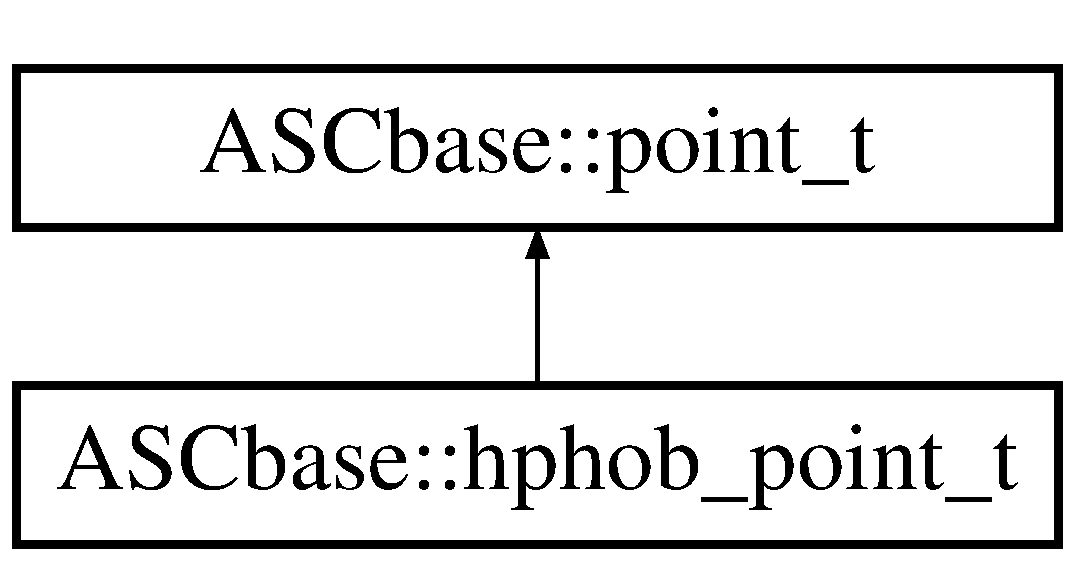
\includegraphics[height=2cm]{classASCbase_1_1hphob__point__t}
\end{center}
\end{figure}
\subsection*{Public Member Functions}
\begin{CompactItemize}
\item 
\textbf{hphob\_\-point\_\-t} (alloc\_\-t a=ALLOC\_\-POSITION)\label{classASCbase_1_1hphob__point__t_e907314b41882b3cb7ba2dee30adb580}

\item 
\textbf{hphob\_\-point\_\-t} (const \bf{hphob\_\-point\_\-t} \&p)\label{classASCbase_1_1hphob__point__t_d1a8e06a18c252ac60c2c5ed9de1b312}

\end{CompactItemize}
\subsection*{Public Attributes}
\begin{CompactItemize}
\item 
std::list$<$ atom\_\-vci $>$ \bf{atoms}\label{classASCbase_1_1hphob__point__t_7e1d90b210cbfb29b6e5fce0cecdd4d8}

\begin{CompactList}\small\item\em Protein heavy atoms that could interact. \item\end{CompactList}\end{CompactItemize}


\subsection{Detailed Description}
Use the base classes position as the computed center \char`\"{}ideal\char`\"{} template points. 



The documentation for this class was generated from the following file:\begin{CompactItemize}
\item 
hphob\_\-point\_\-t.H\end{CompactItemize}

\section{ASCbase::Hphob\-Points Class Reference}
\label{classASCbase_1_1HphobPoints}\index{ASCbase::HphobPoints@{ASCbase::HphobPoints}}
Generate/Load hydrophobic points into a list.  


{\tt \#include $<$Hphob\-Points.H$>$}

\subsection*{Public Member Functions}
\begin{CompactItemize}
\item 
\bf{Hphob\-Points} (std::istream \&in, const uint num\_\-lines, \bf{PDBBase} \&atoms, \bf{PDBBase} \&points)\label{classASCbase_1_1HphobPoints_1b600a08832fe2d624022f19b9e1cbf4}

\begin{CompactList}\small\item\em Default constructor to read hphob points from a sitemap file set. \item\end{CompactList}\item 
\bf{Hphob\-Points} (const \bf{Gen\-Points\-Parameters::hphob\_\-method\_\-t} method\_\-in, const double cluster\_\-diameter\_\-in=3.5, const sphere\_\-sample\_\-level\_\-t sample\_\-level\_\-in=DISCRETE\_\-SPHERE\_\-LEVEL\_\-ZERO)\label{classASCbase_1_1HphobPoints_570ce01d0cd1e8f1d59b93a48a2d4beb}

\begin{CompactList}\small\item\em Default constructor to generate hphob points. \item\end{CompactList}\item 
void \textbf{init\_\-positions\_\-octree} (const my\_\-float\_\-t max\_\-dist, const my\_\-float\_\-t min\_\-side\_\-len, const uint max\_\-numel)\label{classASCbase_1_1HphobPoints_07a9f3bb6d8abbbcb7622e420f912bfc}

\item 
hphob\_\-point\_\-lci \bf{begin} () const \label{classASCbase_1_1HphobPoints_5f178bbf8869f527b842cbda666e8348}

\begin{CompactList}\small\item\em Get a const iterator to the first hphob point. \item\end{CompactList}\item 
hphob\_\-point\_\-lci \bf{end} () const \label{classASCbase_1_1HphobPoints_980fffa0fabdd65b40ceec84c06067fc}

\begin{CompactList}\small\item\em Get a const iterator to one past the last hphob point. \item\end{CompactList}\item 
void \bf{transform} (const my\_\-float\_\-t $\ast$R, const my\_\-float\_\-t $\ast$T)\label{classASCbase_1_1HphobPoints_1dbaaf75ee974e4153e58d4ad0d4abd3}

\begin{CompactList}\small\item\em Transform the hphob points given R and T. \item\end{CompactList}\item 
void \bf{inverse\_\-transform} (const my\_\-float\_\-t $\ast$R, const my\_\-float\_\-t $\ast$T)
\item 
void \bf{revert} ()\label{classASCbase_1_1HphobPoints_65c9e7ac92b005e6c0fc1e9995b94351}

\begin{CompactList}\small\item\em Revert the hphob points as read in or as created? \item\end{CompactList}\item 
hphob\_\-point\_\-lci \textbf{closest\_\-point} (const my\_\-float\_\-t $\ast$pos, my\_\-float\_\-t $\ast$d) const \label{classASCbase_1_1HphobPoints_3ccf4d89489adac1124e765a9493b604}

\item 
my\_\-float\_\-t \bf{compute\_\-RMSD} () const 
\item 
size\_\-t \bf{size} () const 
\begin{CompactList}\small\item\em Number of hphob points. \item\end{CompactList}\item 
bool \textbf{gen\_\-points} (const interact\_\-atoms\_\-vec \&hphob\_\-atoms, const hphob\_\-triad\_\-vec \&hphob\_\-triads, const std::vector$<$ atom\_\-vci $>$ \&rad\_\-atoms, \bf{Bounding\-Volume} $\ast$site\_\-vol)\label{classASCbase_1_1HphobPoints_09a7d1b1f0b101a6adbfa39e8cac7c6e}

\item 
void \textbf{cull\_\-too\_\-close\_\-to\_\-polar} (hbond\_\-fit\_\-pt\_\-vci hbonds\_\-begin, hbond\_\-fit\_\-pt\_\-vci hbonds\_\-end)\label{classASCbase_1_1HphobPoints_6ab0f4ed3f5b7ae8b84288b71ebc8311}

\item 
void \bf{get\_\-current\_\-inverse\_\-3D\_\-transform} (Quaternion $\ast$Q, my\_\-float\_\-t $\ast$T) const 
\end{CompactItemize}
\subsection*{Static Public Member Functions}
\begin{CompactItemize}
\item 
static bool \textbf{atom\_\-is\_\-hphob} (const residue\_\-type res, const atom\_\-type atom, const hphob\_\-triad\_\-t $\ast$$\ast$triad\_\-ptr)\label{classASCbase_1_1HphobPoints_f0aded6fe4d43082ae2eec98b78e4c8b}

\end{CompactItemize}
\subsection*{Private Member Functions}
\begin{CompactItemize}
\item 
bool \textbf{grid\_\-point\_\-methods} (const std::vector$<$ atom\_\-vci $>$ \&rad\_\-atoms, \bf{Bounding\-Volume} $\ast$site\_\-vol)\label{classASCbase_1_1HphobPoints_e735089461a76a86bda11000aa4ee0e7}

\item 
bool \textbf{pseudo\_\-surface\_\-points} (const interact\_\-atoms\_\-vec \&hphob\_\-atoms, const hphob\_\-triad\_\-vec \&hphob\_\-triads, const std::vector$<$ atom\_\-vci $>$ \&rad\_\-atoms, \bf{Bounding\-Volume} $\ast$site\_\-vol)\label{classASCbase_1_1HphobPoints_6d66bc1b44810ac36026c71f7eebcbeb}

\item 
bool \textbf{get\_\-hphobic\_\-atoms} (const std::vector$<$ atom\_\-vci $>$ \&rad\_\-atoms)\label{classASCbase_1_1HphobPoints_8f92e0433c19f069aef713485e1e60d7}

\item 
void \textbf{add\_\-point} (const my\_\-float\_\-t $\ast$pos, \bf{hphob\_\-point\_\-vec} $\ast$pts\_\-vec)\label{classASCbase_1_1HphobPoints_ce1ced666cfe3a8dd21195605609af1d}

\item 
void \textbf{add\_\-point} (const my\_\-float\_\-t $\ast$pos, \bf{hphob\_\-point\_\-list} $\ast$pts\_\-list)\label{classASCbase_1_1HphobPoints_8b20d2a672fc333c8ea5be0f1edf3bcc}

\end{CompactItemize}
\subsection*{Static Private Member Functions}
\begin{CompactItemize}
\item 
static void \textbf{init\_\-hphob\_\-nbrs\_\-tbl} ()\label{classASCbase_1_1HphobPoints_370c8b40fcd5b0ff04da11eac6697463}

\end{CompactItemize}
\subsection*{Private Attributes}
\begin{CompactItemize}
\item 
\bf{Gen\-Points\-Parameters::hphob\_\-method\_\-t} \textbf{method}\label{classASCbase_1_1HphobPoints_11e6f8bf6d7faea419a39d6621f92326}

\item 
sphere\_\-sample\_\-level\_\-t \textbf{sphere\_\-sample\_\-level}\label{classASCbase_1_1HphobPoints_4ff1dda43958356e4730427317c5da34}

\item 
double \textbf{cluster\_\-diameter}\label{classASCbase_1_1HphobPoints_888ec8caee69ebb771ec15f155da32cc}

\item 
\bf{hphob\_\-point\_\-list} \textbf{points}\label{classASCbase_1_1HphobPoints_1c0b6a46ce1914e4d1e6778d6fbb04ad}

\end{CompactItemize}
\subsection*{Static Private Attributes}
\begin{CompactItemize}
\item 
static hphob\_\-triad\_\-map\_\-t \textbf{hphob\_\-nbrs\_\-tbl}\label{classASCbase_1_1HphobPoints_d3f1bba26bfaeb8e8db124fea2c9a646}

\item 
static const my\_\-float\_\-t \bf{MIN\_\-HYDRO\_\-DIST} = 3.0\label{classASCbase_1_1HphobPoints_5c0af7f8cf548ab24531b2fc4d154c56}

\begin{CompactList}\small\item\em closest a template point can be to center of any protein atom \item\end{CompactList}\item 
static const my\_\-float\_\-t \bf{MAX\_\-HYDRO\_\-DIST} = 4.5\label{classASCbase_1_1HphobPoints_39c4760c7bb2cc947393f964a14682cd}

\begin{CompactList}\small\item\em farthest a template point can be from the center of any protein atom \item\end{CompactList}\item 
static const my\_\-float\_\-t \textbf{HPHIL\_\-CUTOFF} = 100\label{classASCbase_1_1HphobPoints_f28d83c9e72324ac0c9e1879a83eb071}

\item 
static const std::string \bf{A\_\-fname} = \char`\"{}Hphob\-Points.C\char`\"{}\label{classASCbase_1_1HphobPoints_df2c547cffadaeb60355a7695a1a330b}

\begin{CompactList}\small\item\em Name of the source file. \item\end{CompactList}\end{CompactItemize}


\subsection{Detailed Description}
Generate/Load hydrophobic points into a list. 



\subsection{Member Function Documentation}
\index{ASCbase::HphobPoints@{ASCbase::Hphob\-Points}!compute_RMSD@{compute\_\-RMSD}}
\index{compute_RMSD@{compute\_\-RMSD}!ASCbase::HphobPoints@{ASCbase::Hphob\-Points}}
\subsubsection{\setlength{\rightskip}{0pt plus 5cm}my\_\-float\_\-t ASCbase::Hphob\-Points::compute\_\-RMSD () const\hspace{0.3cm}{\tt  [inline]}}\label{classASCbase_1_1HphobPoints_747fff02a3a0463f032470212a50e9e6}


Compute the root mean squared deviation (RMSD) between the current and orignial positions of the hydrophobic points \index{ASCbase::HphobPoints@{ASCbase::Hphob\-Points}!get_current_inverse_3D_transform@{get\_\-current\_\-inverse\_\-3D\_\-transform}}
\index{get_current_inverse_3D_transform@{get\_\-current\_\-inverse\_\-3D\_\-transform}!ASCbase::HphobPoints@{ASCbase::Hphob\-Points}}
\subsubsection{\setlength{\rightskip}{0pt plus 5cm}void ASCbase::Hphob\-Points::get\_\-current\_\-inverse\_\-3D\_\-transform (Quaternion $\ast$ {\em Q}, my\_\-float\_\-t $\ast$ {\em T}) const\hspace{0.3cm}{\tt  [inline]}}\label{classASCbase_1_1HphobPoints_130111b0a5617851d7ffde3387c48b80}


Get transform to move current points to original position of the points \index{ASCbase::HphobPoints@{ASCbase::Hphob\-Points}!inverse_transform@{inverse\_\-transform}}
\index{inverse_transform@{inverse\_\-transform}!ASCbase::HphobPoints@{ASCbase::Hphob\-Points}}
\subsubsection{\setlength{\rightskip}{0pt plus 5cm}void ASCbase::Hphob\-Points::inverse\_\-transform (const my\_\-float\_\-t $\ast$ {\em R}, const my\_\-float\_\-t $\ast$ {\em T})\hspace{0.3cm}{\tt  [inline]}}\label{classASCbase_1_1HphobPoints_116528abe8dfc536c786ac885e87dc02}


Transform the hphob points by the inverse transform of the transform given by R and T \index{ASCbase::HphobPoints@{ASCbase::Hphob\-Points}!size@{size}}
\index{size@{size}!ASCbase::HphobPoints@{ASCbase::Hphob\-Points}}
\subsubsection{\setlength{\rightskip}{0pt plus 5cm}size\_\-t ASCbase::Hphob\-Points::size () const\hspace{0.3cm}{\tt  [inline]}}\label{classASCbase_1_1HphobPoints_b1837926d048082c5aaf03d5cd3346cd}


Number of hphob points. 

A helper function since list iterators do not support addition and subtraction 

The documentation for this class was generated from the following files:\begin{CompactItemize}
\item 
Hphob\-Points.H\item 
Hphob\-Points.C\end{CompactItemize}

\section{ASCbase::geometry::i\-Circle Class Reference}
\label{classASCbase_1_1geometry_1_1iCircle}\index{ASCbase::geometry::iCircle@{ASCbase::geometry::iCircle}}
Computational representation of an analytical intersection circle.  


{\tt \#include $<$sphere.H$>$}

\subsection*{Public Member Functions}
\begin{CompactItemize}
\item 
\bf{i\-Circle} (const my\_\-float\_\-t $\ast$C, my\_\-float\_\-t R, const my\_\-float\_\-t $\ast$N, const std::vector$<$ \bf{arc\_\-t} $>$ \&initial\_\-arcs)\label{classASCbase_1_1geometry_1_1iCircle_dc2d91b17a31b6efdf2507fbbd96adbf}

\begin{CompactList}\small\item\em Simple copy constructor. \item\end{CompactList}\item 
\bf{i\-Circle} (const \bf{i\-Circle} \&src)\label{classASCbase_1_1geometry_1_1iCircle_a6c96857415afe3683f6ef6d51dd4d8c}

\begin{CompactList}\small\item\em Simple assignment function (operator). \item\end{CompactList}\item 
const \bf{i\-Circle} \& \bf{operator=} (const \bf{i\-Circle} \&src)\label{classASCbase_1_1geometry_1_1iCircle_afc268254b2b9d9f6f61a918a2a52dfc}

\begin{CompactList}\small\item\em Remove the part of self that overlaps with the other \doxyref{i\-Circle}{p.}{classASCbase_1_1geometry_1_1iCircle}. \item\end{CompactList}\item 
void \textbf{remove\_\-overlap} (const \bf{i\-Circle} \&other)\label{classASCbase_1_1geometry_1_1iCircle_cdc19b475429b75f5513d4eae4b17749}

\item 
bool \bf{project\_\-point} (const my\_\-float\_\-t $\ast$pt, my\_\-float\_\-t $\ast$proj\_\-pt, my\_\-float\_\-t $\ast$sq\_\-dist, const my\_\-float\_\-t tol=1.0)\label{classASCbase_1_1geometry_1_1iCircle_214a76a297e276e2c0d6f4b07d34c731}

\begin{CompactList}\small\item\em Project point to the intersection circle. \item\end{CompactList}\item 
bool \bf{full\_\-circle} () const 
\item 
uint \bf{num\_\-final\_\-arcs} () const \label{classASCbase_1_1geometry_1_1iCircle_b3746f127fd9a5e4eda03b91e61c1325}

\begin{CompactList}\small\item\em Get the number of final arcs. \item\end{CompactList}\item 
std::vector$<$ \bf{arc\_\-t} $>$::const\_\-iterator \bf{final\_\-arcs\_\-begin} () const \label{classASCbase_1_1geometry_1_1iCircle_afd4529a5f5d5fdc4bb8828a5da80e38}

\begin{CompactList}\small\item\em Get a const iterator to the first final arc. \item\end{CompactList}\item 
std::vector$<$ \bf{arc\_\-t} $>$::const\_\-iterator \bf{final\_\-arcs\_\-end} () const \label{classASCbase_1_1geometry_1_1iCircle_218c0440280ff4520f9f8e40f35688dc}

\begin{CompactList}\small\item\em Get a const iterator to one past the last final arc. \item\end{CompactList}\end{CompactItemize}
\subsection*{Private Member Functions}
\begin{CompactItemize}
\item 
void \bf{do\_\-copy} (const \bf{i\-Circle} \&src)\label{classASCbase_1_1geometry_1_1iCircle_54491e02cadfba9d450243eb0012d5b6}

\begin{CompactList}\small\item\em $<$ Simple copy function \item\end{CompactList}\end{CompactItemize}
\subsection*{Private Attributes}
\begin{CompactItemize}
\item 
bool \textbf{A\_\-full\_\-circle}\label{classASCbase_1_1geometry_1_1iCircle_2ddf6cfc4477e5bdba558719c78e7f91}

\item 
\bf{plane\_\-t} \textbf{A\_\-plane}\label{classASCbase_1_1geometry_1_1iCircle_6ae4379845c47b1fbad97a289f15fda0}

\item 
std::vector$<$ \bf{arc\_\-t} $>$ \textbf{A\_\-final\_\-arcs}\label{classASCbase_1_1geometry_1_1iCircle_1614741330df5d735e025d3cdffc035c}

\end{CompactItemize}
\subsection*{Classes}
\begin{CompactItemize}
\item 
struct \bf{point\_\-type}
\begin{CompactList}\small\item\em Structure to allow storage of 3D pts in a vector. \item\end{CompactList}\end{CompactItemize}


\subsection{Detailed Description}
Computational representation of an analytical intersection circle. 

NOTE: the contains function is from the sphere\_\-t class

NOTE: some functions from the sphere\_\-t class might not be applicable to the \doxyref{i\-Circle}{p.}{classASCbase_1_1geometry_1_1iCircle} idea -- be careful. As an example, project\_\-point is not overloaded and will project to sphere not necessarily on the circle. 



\subsection{Member Function Documentation}
\index{ASCbase::geometry::iCircle@{ASCbase::geometry::i\-Circle}!full_circle@{full\_\-circle}}
\index{full_circle@{full\_\-circle}!ASCbase::geometry::iCircle@{ASCbase::geometry::i\-Circle}}
\subsubsection{\setlength{\rightskip}{0pt plus 5cm}bool ASCbase::geometry::i\-Circle::full\_\-circle () const\hspace{0.3cm}{\tt  [inline]}}\label{classASCbase_1_1geometry_1_1iCircle_a3821e31fe1ca72a92c040bebd0cbab7}


Returns true if this intersection circle does not intersect with the cutting plane or any other intersection circle 

The documentation for this class was generated from the following file:\begin{CompactItemize}
\item 
sphere.H\end{CompactItemize}

\section{ASCbase::geometry::i\-Circle::point\_\-type Struct Reference}
\label{structASCbase_1_1geometry_1_1iCircle_1_1point__type}\index{ASCbase::geometry::iCircle::point_type@{ASCbase::geometry::iCircle::point\_\-type}}
Structure to allow storage of 3D pts in a vector.  


{\tt \#include $<$sphere.H$>$}

\subsection*{Public Attributes}
\begin{CompactItemize}
\item 
my\_\-float\_\-t \textbf{pt} [3]\label{structASCbase_1_1geometry_1_1iCircle_1_1point__type_b2fba8f10a57aa81097fe33f7026628f}

\end{CompactItemize}


\subsection{Detailed Description}
Structure to allow storage of 3D pts in a vector. 



The documentation for this struct was generated from the following file:\begin{CompactItemize}
\item 
sphere.H\end{CompactItemize}

\section{ASCbase::Identity\-Alignment Class Reference}
\label{classASCbase_1_1IdentityAlignment}\index{ASCbase::IdentityAlignment@{ASCbase::IdentityAlignment}}
{\tt \#include $<$Identity\-Alignment.H$>$}

\subsection*{Public Member Functions}
\begin{CompactItemize}
\item 
\bf{Identity\-Alignment} ()\label{classASCbase_1_1IdentityAlignment_797fcc9db55bc0f73d3c07355627983f}

\begin{CompactList}\small\item\em Cstor. \item\end{CompactList}\item 
virtual \bf{$\sim$Identity\-Alignment} ()\label{classASCbase_1_1IdentityAlignment_2fb1a7e4efddaba4b1c392884aab7782}

\begin{CompactList}\small\item\em basic destruction \item\end{CompactList}\item 
template$<$typename align\_\-T$>$ bool \bf{align} (\bf{Model\-Sitemap} $\ast$query\_\-site, \bf{Sitemap} \&dset\_\-site, std::vector$<$ align\_\-T $>$ $\ast$alignments)\label{classASCbase_1_1IdentityAlignment_3ac828753736d937a23ff2f92394ecc3}

\begin{CompactList}\small\item\em Required alignment method. \item\end{CompactList}\end{CompactItemize}


\subsection{Detailed Description}
Used when user wants to score the sites as given -- generally not useful in the case of a standard screening dataset 



The documentation for this class was generated from the following file:\begin{CompactItemize}
\item 
Identity\-Alignment.H\end{CompactItemize}

\section{ASCbase::IK\_\-tests Class Reference}
\label{classASCbase_1_1IK__tests}\index{ASCbase::IK_tests@{ASCbase::IK\_\-tests}}
Testing/Validation class for surface deformations and hbonds moving.  


{\tt \#include $<$IK\_\-tests.H$>$}

\subsection*{Public Member Functions}
\begin{CompactItemize}
\item 
\bf{IK\_\-tests} (const \bf{Search\-Parameters} \&args)\label{classASCbase_1_1IK__tests_89ac913085506be49f734d9d3fbc5d19}

\begin{CompactList}\small\item\em Only allowed Cstor for search\_\-sitemaps. \item\end{CompactList}\item 
\bf{$\sim$IK\_\-tests} ()\label{classASCbase_1_1IK__tests_280f1a906f3d73ddd2037c2bbbaf0533}

\begin{CompactList}\small\item\em Free up the user\_\-args structure. \item\end{CompactList}\item 
void \bf{test\_\-moving\_\-stuff} (const \bf{Search\-Parameters} \&args\_\-in)
\begin{CompactList}\small\item\em Big messy test function. \item\end{CompactList}\item 
void \bf{run} (\bf{Model\-Sitemap} $\ast$model\_\-site, const \bf{Dbase\-Sitemap} \&dbase\_\-site, \bf{rigid\_\-align\_\-t} $\ast$align, const std::string db\_\-struct\_\-id, std::ostream \&out)
\begin{CompactList}\small\item\em Run flexibility using the current orientation of the model site. \item\end{CompactList}\item 
my\_\-float\_\-t \textbf{compute\_\-initial\_\-atomic\_\-rmsd} (\bf{Model\-Sitemap} $\ast$model\_\-site, const \bf{Dbase\-Sitemap} \&dbase\_\-site, \bf{rigid\_\-align\_\-t} $\ast$align)\label{classASCbase_1_1IK__tests_5748368e2908160b96bcabb654fdcbe6}

\end{CompactItemize}
\subsection*{Static Public Member Functions}
\begin{CompactItemize}
\item 
static const my\_\-float\_\-t \textbf{max\_\-atom\_\-dist\_\-for\_\-checking\_\-vdw\_\-overlap} ()\label{classASCbase_1_1IK__tests_06c9e7b5b2840ca8d74bd6582d883c83}

\end{CompactItemize}
\subsection*{Private Attributes}
\begin{CompactItemize}
\item 
\bf{Sites\-Score\-Base} $\ast$ \textbf{A\_\-site\_\-score\_\-p}\label{classASCbase_1_1IK__tests_d39cab900cbb424c333c3c51dbbecc0c}

\item 
bool \textbf{A\_\-uses\_\-site\_\-surface}\label{classASCbase_1_1IK__tests_b047df9991ddc5f5cfbdd35b245dac06}

\item 
bool \bf{A\_\-uses\_\-hbond\_\-surfaces}\label{classASCbase_1_1IK__tests_d7947e90a6605298f42be161830ec40e}

\begin{CompactList}\small\item\em Art\-Surf includes site surface. \item\end{CompactList}\item 
bool \bf{A\_\-hbond\_\-caps\_\-ICP}\label{classASCbase_1_1IK__tests_c47ea936905f2ff6b2815129ad205395}

\begin{CompactList}\small\item\em Art\-Surt includes hbond caps. \item\end{CompactList}\item 
my\_\-float\_\-t \textbf{A\_\-ICP\_\-surf\_\-pt\_\-W}\label{classASCbase_1_1IK__tests_f66ad10a0abe61813e9cc2dd01887cb1}

\item 
my\_\-float\_\-t \textbf{A\_\-ICP\_\-hb\_\-cap\_\-pt\_\-W}\label{classASCbase_1_1IK__tests_1096e6e78d144f78bf891188b0a5e18f}

\end{CompactItemize}
\subsection*{Static Private Attributes}
\begin{CompactItemize}
\item 
static const my\_\-float\_\-t \bf{MAX\_\-ATOM\_\-DIST\_\-TO\_\-CHECK\_\-VDW\_\-OVERLAP} = 4.5\label{classASCbase_1_1IK__tests_229bfd4bf67a0a8a73322015a0307c22}

\begin{CompactList}\small\item\em Maximum distance between any 2 to require checking of intersection of Van der Waals spheres. \item\end{CompactList}\item 
static const std::string \textbf{A\_\-fname} = \char`\"{}IK\_\-tests.C\char`\"{}\label{classASCbase_1_1IK__tests_2f41807950842f871a832e69ae666921}

\end{CompactItemize}


\subsection{Detailed Description}
Testing/Validation class for surface deformations and hbonds moving. 



\subsection{Member Function Documentation}
\index{ASCbase::IK_tests@{ASCbase::IK\_\-tests}!run@{run}}
\index{run@{run}!ASCbase::IK_tests@{ASCbase::IK\_\-tests}}
\subsubsection{\setlength{\rightskip}{0pt plus 5cm}void IK\_\-tests::run (\bf{Model\-Sitemap} $\ast$ {\em model\_\-site}, const \bf{Dbase\-Sitemap} \& {\em dbase\_\-site}, \bf{rigid\_\-align\_\-t} $\ast$ {\em align}, const std::string {\em db\_\-struct\_\-id}, std::ostream \& {\em out})}\label{classASCbase_1_1IK__tests_fac5e4fb00a62ec37cc72f53ebb20cfd}


Run flexibility using the current orientation of the model site. 

Assumption: ICP steps have been done to get binding site into a good correspondence 

std::cout $<$$<$ vdw\_\-rad\_\-sum - atomic\_\-dist $<$$<$ \char`\"{} \char`\"{}; \index{ASCbase::IK_tests@{ASCbase::IK\_\-tests}!test_moving_stuff@{test\_\-moving\_\-stuff}}
\index{test_moving_stuff@{test\_\-moving\_\-stuff}!ASCbase::IK_tests@{ASCbase::IK\_\-tests}}
\subsubsection{\setlength{\rightskip}{0pt plus 5cm}void IK\_\-tests::test\_\-moving\_\-stuff (const \bf{Search\-Parameters} \& {\em args\_\-in})}\label{classASCbase_1_1IK__tests_f4fdeb2d068d4b958a999d2c2673c183}


Big messy test function. 

Assumes that args() contains both query and db sites (i.e. no dataset searching) 

The documentation for this class was generated from the following files:\begin{CompactItemize}
\item 
IK\_\-tests.H\item 
IK\_\-tests.C\end{CompactItemize}

\section{ASCbase::Initial\-Alignments\-Base Class Reference}
\label{classASCbase_1_1InitialAlignmentsBase}\index{ASCbase::InitialAlignmentsBase@{ASCbase::InitialAlignmentsBase}}
Base class for initial alignment(s) of site maps / binding sites.  


{\tt \#include $<$Initial\-Alignments\-Base.H$>$}

\subsection*{Public Member Functions}
\begin{CompactItemize}
\item 
\bf{Initial\-Alignments\-Base} ()\label{classASCbase_1_1InitialAlignmentsBase_5980fc0808725ed85537211cb846a527}

\begin{CompactList}\small\item\em Cstor. \item\end{CompactList}\item 
virtual \bf{$\sim$Initial\-Alignments\-Base} ()\label{classASCbase_1_1InitialAlignmentsBase_2bf277ae7d263c8116508e5e440c1896}

\begin{CompactList}\small\item\em basic destruction \item\end{CompactList}\item 
template$<$typename align\_\-T$>$ bool \textbf{align} (\bf{Sitemap} \&dset\_\-site, std::vector$<$ align\_\-T $>$ $\ast$alignments)\label{classASCbase_1_1InitialAlignmentsBase_7cfb90c844039c31f14e07fb3d814bb5}

\end{CompactItemize}


\subsection{Detailed Description}
Base class for initial alignment(s) of site maps / binding sites. 



The documentation for this class was generated from the following file:\begin{CompactItemize}
\item 
Initial\-Alignments\-Base.H\end{CompactItemize}

\section{ASCbase::interact\_\-point\_\-t Class Reference}
\label{classASCbase_1_1interact__point__t}\index{ASCbase::interact_point_t@{ASCbase::interact\_\-point\_\-t}}
Interactions points.  


{\tt \#include $<$interact\_\-point\_\-t.H$>$}

Inheritance diagram for ASCbase::interact\_\-point\_\-t::\begin{figure}[H]
\begin{center}
\leavevmode
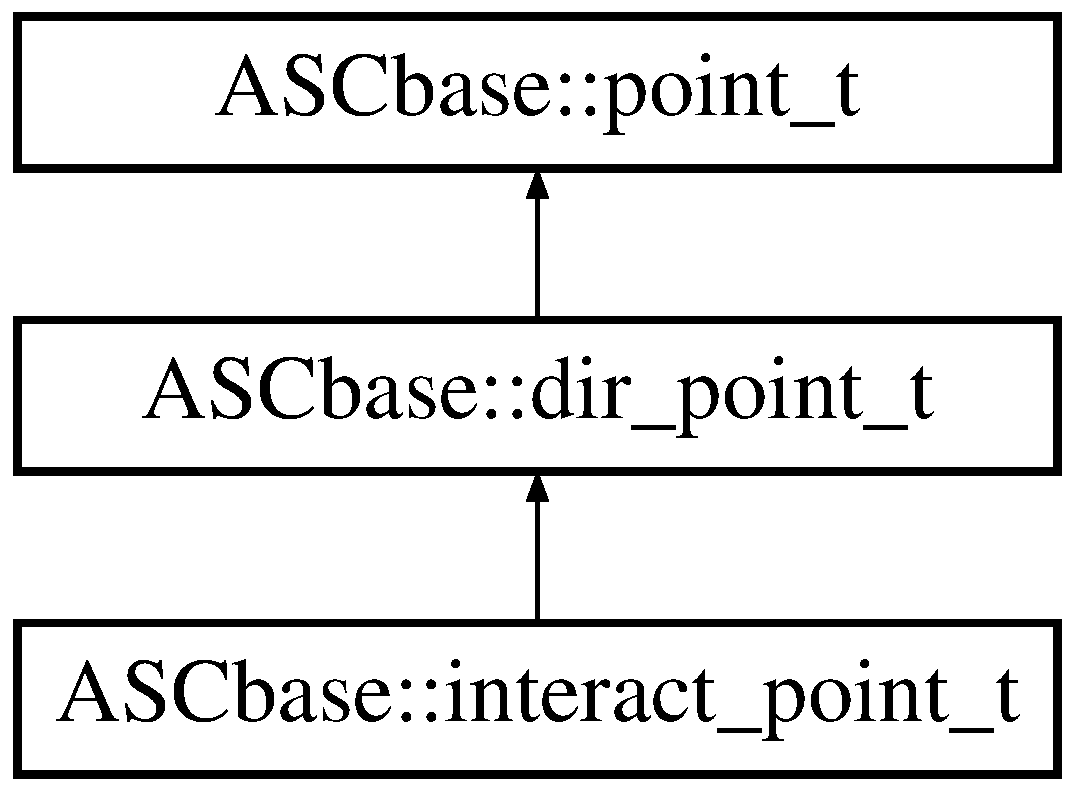
\includegraphics[height=3cm]{classASCbase_1_1interact__point__t}
\end{center}
\end{figure}
\subsection*{Public Member Functions}
\begin{CompactItemize}
\item 
\textbf{interact\_\-point\_\-t} (alloc\_\-t a=ALLOC\_\-POSITION)\label{classASCbase_1_1interact__point__t_847336b4146fb570f5dbf56a0cd1d2dc}

\item 
\textbf{interact\_\-point\_\-t} (const \bf{interact\_\-point\_\-t} \&p)\label{classASCbase_1_1interact__point__t_2d6a71e803d863c51a4fbd9d141c563c}

\item 
const \bf{interact\_\-point\_\-t} \& \textbf{operator=} (const \bf{interact\_\-point\_\-t} \&p)\label{classASCbase_1_1interact__point__t_b4f20ff04e85bf54b0ef6652ff899c04}

\end{CompactItemize}
\subsection*{Static Public Member Functions}
\begin{CompactItemize}
\item 
static bool \textbf{cmp} (const \bf{interact\_\-point\_\-t} \&A, const \bf{interact\_\-point\_\-t} \&B)\label{classASCbase_1_1interact__point__t_422857df1c11412c9c2b750f9d2d3ee2}

\end{CompactItemize}
\subsection*{Public Attributes}
\begin{CompactItemize}
\item 
interaction\-Type \bf{act\_\-type}\label{classASCbase_1_1interact__point__t_63eee3d009abf146282a6a8bf73bbaec}

\begin{CompactList}\small\item\em Interaction type of the points. \item\end{CompactList}\end{CompactItemize}
\subsection*{Private Member Functions}
\begin{CompactItemize}
\item 
void \textbf{do\_\-copy} (const \bf{interact\_\-point\_\-t} \&p)\label{classASCbase_1_1interact__point__t_01ba09e2cc58d89156b62a2398e24de1}

\end{CompactItemize}


\subsection{Detailed Description}
Interactions points. 



The documentation for this class was generated from the following file:\begin{CompactItemize}
\item 
interact\_\-point\_\-t.H\end{CompactItemize}

\section{ASCbase::Match\-Triangles Class Reference}
\label{classASCbase_1_1MatchTriangles}\index{ASCbase::MatchTriangles@{ASCbase::MatchTriangles}}
Registration of sitemaps based on close 3 point alignments.  


{\tt \#include $<$Match\-Triangles.H$>$}

\subsection*{Public Member Functions}
\begin{CompactItemize}
\item 
\bf{Match\-Triangles} (const my\_\-float\_\-t dmetol\_\-in, const my\_\-float\_\-t lsetol\_\-in, const bool allow\_\-hphob\_\-triangles)
\begin{CompactList}\small\item\em Cstor. \item\end{CompactList}\item 
virtual \bf{$\sim$Match\-Triangles} ()\label{classASCbase_1_1MatchTriangles_2c1b59400cb3b11d304f8ac9fe4446e1}

\begin{CompactList}\small\item\em basic destruction \item\end{CompactList}\item 
template$<$typename align\_\-T$>$ bool \bf{align} (\bf{Model\-Sitemap} $\ast$query\_\-site, \bf{Sitemap} \&dset\_\-site, std::vector$<$ align\_\-T $>$ $\ast$alignments)
\begin{CompactList}\small\item\em Run to generate the 3pt rigid alignments. \item\end{CompactList}\end{CompactItemize}
\subsection*{Private Member Functions}
\begin{CompactItemize}
\item 
template$<$typename align\_\-T$>$ void \textbf{compute\_\-triangles} (std::vector$<$ uint $>$ $\ast$arr\_\-p, int index, int length, std::vector$<$ align\_\-T $>$ $\ast$alignments)\label{classASCbase_1_1MatchTriangles_147928ad10a438af6c6e6ee6cefe10df}

\item 
int \bf{get\_\-best\_\-correspondence} (const \bf{triangle\_\-t} \&model\_\-tri, const \bf{triangle\_\-t} \&search\_\-tri)
\begin{CompactList}\small\item\em Find the best correspondence between a given model and search triangle. \item\end{CompactList}\item 
bool \bf{Three\-Pt\-Least\-Squares} (const \bf{triangle\_\-t} \&A, const \bf{triangle\_\-t} \&B, Quaternion $\ast$Q, my\_\-float\_\-t $\ast$R, my\_\-float\_\-t $\ast$T)
\begin{CompactList}\small\item\em Wrapper to get the least squares fit for two triangles. \item\end{CompactList}\item 
bool \textbf{get\_\-triangles} (\bf{triangle\_\-t} $\ast$target\_\-tri, const std::vector$<$ uint $>$ \&arr, bucket\_\-vci $\ast$bucket\_\-begin, bucket\_\-vci $\ast$bucket\_\-end)\label{classASCbase_1_1MatchTriangles_6212c1fe978ef723724ed5029963e109}

\end{CompactItemize}
\subsection*{Private Attributes}
\begin{CompactItemize}
\item 
\bf{Model\-Sitemap} $\ast$ \textbf{A\_\-model}\label{classASCbase_1_1MatchTriangles_4a2674b892098a9041d2d64240545d3d}

\item 
my\_\-float\_\-t \textbf{target\_\-centroid} [3]\label{classASCbase_1_1MatchTriangles_3c8d67e4f6f23bb114deaffd0e983c06}

\item 
interact\_\-pts\_\-vci \textbf{A\_\-targ\_\-pts\_\-beg}\label{classASCbase_1_1MatchTriangles_db2be75b7d41089ed59a31b0fd6ab4d0}

\item 
my\_\-float\_\-t \bf{dmetol\_\-2}\label{classASCbase_1_1MatchTriangles_285278f41b70244a22984cf328522494}

\begin{CompactList}\small\item\em Square of avg distance metric error tolerance. \item\end{CompactList}\item 
my\_\-float\_\-t \bf{lsetol\_\-2}\label{classASCbase_1_1MatchTriangles_4f725552c68b6de6e1d49a9796a3165b}

\begin{CompactList}\small\item\em Square of avg least squares pt correspondence tol. \item\end{CompactList}\item 
bool \textbf{A\_\-allow\_\-hphob\_\-triangles}\label{classASCbase_1_1MatchTriangles_0987b2902ceeac3e785e3a44db49f6f0}

\end{CompactItemize}
\subsection*{Static Private Attributes}
\begin{CompactItemize}
\item 
static const std::string \bf{\_\-fname} = \char`\"{}Match\-Triangles.C\char`\"{}\label{classASCbase_1_1MatchTriangles_263da86497b71a67e4cb0b14356e830d}

\begin{CompactList}\small\item\em Name of the source file. \item\end{CompactList}\item 
static const int \bf{permutations} [6][3]
\begin{CompactList}\small\item\em Permutations of edges. \item\end{CompactList}\item 
static const int \bf{point\_\-permutations} [6][3]
\begin{CompactList}\small\item\em Permutations of vertices. \item\end{CompactList}\item 
static const int \bf{ACCEPTOR\_\-ACCEPTOR} = 2\label{classASCbase_1_1MatchTriangles_987dee7263175dc5dac58309ca26d4eb}

\begin{CompactList}\small\item\em 2 $\ast$ ACCEPTOR \item\end{CompactList}\item 
static const int \bf{DONOR\_\-DONOR} = 8\label{classASCbase_1_1MatchTriangles_b78b92259f4ef3245675fdf17a21f6c9}

\begin{CompactList}\small\item\em 2 $\ast$ DONOR \item\end{CompactList}\item 
static const int \bf{HYDROPHOB\_\-HYDROPHOB} = 32\label{classASCbase_1_1MatchTriangles_ff621328272ce0e2c143efe4315feb9c}

\begin{CompactList}\small\item\em 2 $\ast$ HYDROPHOB \item\end{CompactList}\item 
static const int \bf{ACCEPTOR\_\-DONOR} = 5\label{classASCbase_1_1MatchTriangles_ade24f76f84d429853f48e41208db45e}

\begin{CompactList}\small\item\em ACCEPTOR + DONOR. \item\end{CompactList}\item 
static const int \bf{ACCEPTOR\_\-DONEPTOR} = 65\label{classASCbase_1_1MatchTriangles_4c4b4779b05e824be2960a0a6ba525f8}

\begin{CompactList}\small\item\em ACCEPTOR + DONEPTOR. \item\end{CompactList}\item 
static const int \bf{DONOR\_\-DONEPTOR} = 68\label{classASCbase_1_1MatchTriangles_7816e470f2da8b31bfe68f635a84870f}

\begin{CompactList}\small\item\em DONOR + DONEPTOR. \item\end{CompactList}\item 
static const int \bf{DONEPTOR\_\-DONEPTOR} = 128\label{classASCbase_1_1MatchTriangles_152f1eff01e619c50b2361c394330a63}

\begin{CompactList}\small\item\em DONEPTOR + DONEPTOR. \item\end{CompactList}\end{CompactItemize}


\subsection{Detailed Description}
Registration of sitemaps based on close 3 point alignments. 



\subsection{Constructor \& Destructor Documentation}
\index{ASCbase::MatchTriangles@{ASCbase::Match\-Triangles}!MatchTriangles@{MatchTriangles}}
\index{MatchTriangles@{MatchTriangles}!ASCbase::MatchTriangles@{ASCbase::Match\-Triangles}}
\subsubsection{\setlength{\rightskip}{0pt plus 5cm}Match\-Triangles::Match\-Triangles (const my\_\-float\_\-t {\em dmetol\_\-in}, const my\_\-float\_\-t {\em lsetol\_\-in}, const bool {\em allow\_\-hphob\_\-triangles})}\label{classASCbase_1_1MatchTriangles_29b1ab95b85c05e891ecbdc6700e5926}


Cstor. 

\begin{Desc}
\item[Parameters:]
\begin{description}
\item[{\em dmetol\_\-in}]Max tolerated average distance metric error \item[{\em lsetol\_\-in}]Max tolerated average least squares error \item[{\em allow\_\-hphob\_\-triangles}]If false, triangles must contain at least 1 hydrogen bond \end{description}
\end{Desc}


\subsection{Member Function Documentation}
\index{ASCbase::MatchTriangles@{ASCbase::Match\-Triangles}!align@{align}}
\index{align@{align}!ASCbase::MatchTriangles@{ASCbase::Match\-Triangles}}
\subsubsection{\setlength{\rightskip}{0pt plus 5cm}template$<$typename align\_\-T$>$ bool ASCbase::Match\-Triangles::align (\bf{Model\-Sitemap} $\ast$ {\em query\_\-site}, \bf{Sitemap} \& {\em dset\_\-site}, std::vector$<$ align\_\-T $>$ $\ast$ {\em alignments})\hspace{0.3cm}{\tt  [inline]}}\label{classASCbase_1_1MatchTriangles_e1a93a3866983cd03a85ebc19cca5908}


Run to generate the 3pt rigid alignments. 

\begin{Desc}
\item[Parameters:]
\begin{description}
\item[{\em dset\_\-site}]Pointer to the \char`\"{}second\char`\"{} sitemap \item[{\em alignments}]Pointer to the vector holding found correspondences \end{description}
\end{Desc}
\index{ASCbase::MatchTriangles@{ASCbase::Match\-Triangles}!get_best_correspondence@{get\_\-best\_\-correspondence}}
\index{get_best_correspondence@{get\_\-best\_\-correspondence}!ASCbase::MatchTriangles@{ASCbase::Match\-Triangles}}
\subsubsection{\setlength{\rightskip}{0pt plus 5cm}int Match\-Triangles::get\_\-best\_\-correspondence (const \bf{triangle\_\-t} \& {\em model\_\-tri}, const \bf{triangle\_\-t} \& {\em search\_\-tri})\hspace{0.3cm}{\tt  [private]}}\label{classASCbase_1_1MatchTriangles_90fabfb57f81c9a8366434de82984762}


Find the best correspondence between a given model and search triangle. 

For each (6) permuation of the vertices of the search triangle see if the corresponding vertices (of the model triangle) are compatible. If they are, determine the average difference of the corresponding edge lengths. The permutation with the lowest average difference is taken to be the one of choice. If there is no permutation with corresponding vertices with an average difference of edge lengths under the given tolerance, return -1 (no correspondence).

\begin{Desc}
\item[Parameters:]
\begin{description}
\item[{\em model\_\-tri}]Reference to a model triangle \item[{\em search\_\-tri}]Reference to a search triangle \end{description}
\end{Desc}
\begin{Desc}
\item[Returns:]0--5 depending which permutation is closest match, -1 if none \end{Desc}
\index{ASCbase::MatchTriangles@{ASCbase::Match\-Triangles}!ThreePtLeastSquares@{ThreePtLeastSquares}}
\index{ThreePtLeastSquares@{ThreePtLeastSquares}!ASCbase::MatchTriangles@{ASCbase::Match\-Triangles}}
\subsubsection{\setlength{\rightskip}{0pt plus 5cm}bool Match\-Triangles::Three\-Pt\-Least\-Squares (const \bf{triangle\_\-t} \& {\em A}, const \bf{triangle\_\-t} \& {\em B}, Quaternion $\ast$ {\em Q}, my\_\-float\_\-t $\ast$ {\em R}, my\_\-float\_\-t $\ast$ {\em T})\hspace{0.3cm}{\tt  [private]}}\label{classASCbase_1_1MatchTriangles_434d4cfe074a18dd8d79b46b5585b559}


Wrapper to get the least squares fit for two triangles. 

Get a weighted least squares fit to align A to B. That is, A is moved to the reference frame of B.

\begin{Desc}
\item[Parameters:]
\begin{description}
\item[{\em A}]Triangle to move to the reference point of B \item[{\em B}]Triangle to align A to \item[{\em res}]Pointer to a results structure (holds the transformation) \end{description}
\end{Desc}
\begin{Desc}
\item[Returns:]True implies least squares had error below tolerance \end{Desc}


\subsection{Member Data Documentation}
\index{ASCbase::MatchTriangles@{ASCbase::Match\-Triangles}!permutations@{permutations}}
\index{permutations@{permutations}!ASCbase::MatchTriangles@{ASCbase::Match\-Triangles}}
\subsubsection{\setlength{\rightskip}{0pt plus 5cm}const int \bf{Match\-Triangles::permutations}\hspace{0.3cm}{\tt  [static, private]}}\label{classASCbase_1_1MatchTriangles_ef9e8c25707ff5d109fc2f93d00be198}


\textbf{Initial value:}

\begin{Code}\begin{verbatim} 
{ { 0, 1, 2 },
  { 0, 2, 1 },
  { 1, 0, 2 },
  { 1, 2, 0 },
  { 2, 0, 1 },
  { 2, 1, 0 } }
\end{verbatim}\end{Code}
Permutations of edges. 

\index{ASCbase::MatchTriangles@{ASCbase::Match\-Triangles}!point_permutations@{point\_\-permutations}}
\index{point_permutations@{point\_\-permutations}!ASCbase::MatchTriangles@{ASCbase::Match\-Triangles}}
\subsubsection{\setlength{\rightskip}{0pt plus 5cm}const int \bf{Match\-Triangles::point\_\-permutations}\hspace{0.3cm}{\tt  [static, private]}}\label{classASCbase_1_1MatchTriangles_5249b60afc22af79841be9345cf6c98e}


\textbf{Initial value:}

\begin{Code}\begin{verbatim} 
{ { 0, 1, 2 },
  { 1, 0, 2 },
  { 2, 1, 0 },
  { 1, 2, 0 },
  { 2, 0, 1 },
  { 0, 2, 1 } }
\end{verbatim}\end{Code}
Permutations of vertices. 



The documentation for this class was generated from the following files:\begin{CompactItemize}
\item 
Match\-Triangles.H\item 
Match\-Triangles.C\end{CompactItemize}

\section{ASCbase::model\_\-hbond\_\-surf\_\-t Class Reference}
\label{classASCbase_1_1model__hbond__surf__t}\index{ASCbase::model_hbond_surf_t@{ASCbase::model\_\-hbond\_\-surf\_\-t}}
{\tt \#include $<$Model\-Hbond\-Surfaces.H$>$}

Inheritance diagram for ASCbase::model\_\-hbond\_\-surf\_\-t::\begin{figure}[H]
\begin{center}
\leavevmode
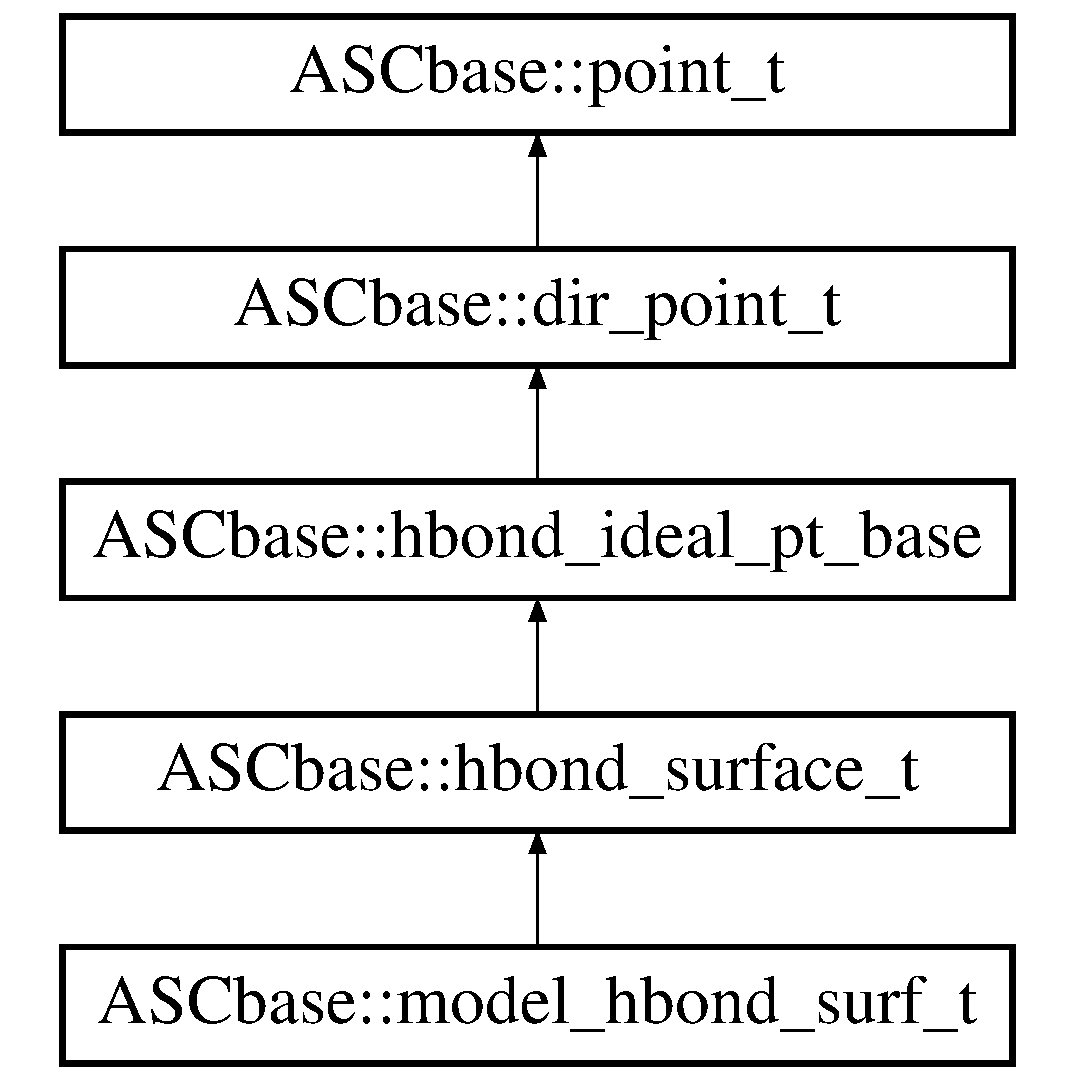
\includegraphics[height=5cm]{classASCbase_1_1model__hbond__surf__t}
\end{center}
\end{figure}
\subsection*{Public Member Functions}
\begin{CompactItemize}
\item 
\textbf{model\_\-hbond\_\-surf\_\-t} (const std::string \&data\_\-line, \bf{PDBBase} \&prot\_\-atoms, const uint level=2)\label{classASCbase_1_1model__hbond__surf__t_cb646a3dbc03f4990450144a918753a8}

\item 
\textbf{model\_\-hbond\_\-surf\_\-t} (const \bf{model\_\-hbond\_\-surf\_\-t} \&src)\label{classASCbase_1_1model__hbond__surf__t_c6978b9984df3bdd11e5b492600468c2}

\item 
\bf{model\_\-hbond\_\-surf\_\-t} \& \textbf{operator=} (const \bf{model\_\-hbond\_\-surf\_\-t} \&src)\label{classASCbase_1_1model__hbond__surf__t_01930d6fccfbfb3c509b686060699606}

\item 
void \textbf{transform} (const my\_\-float\_\-t $\ast$R, const my\_\-float\_\-t $\ast$T)\label{classASCbase_1_1model__hbond__surf__t_65d5a73c0ffcbada1c8496c81a43929a}

\item 
void \textbf{inverse\_\-transform} (const my\_\-float\_\-t $\ast$R, const my\_\-float\_\-t $\ast$T)\label{classASCbase_1_1model__hbond__surf__t_b0ebe991b54fb1b3247a4a716a0673d4}

\item 
void \textbf{revert} ()\label{classASCbase_1_1model__hbond__surf__t_da904de58db5258030d9144908f915c6}

\item 
void \bf{compute\_\-best\_\-terms} (std::vector$<$ \bf{hbond\_\-surface\_\-t} $>$::iterator surfs\_\-begin, std::vector$<$ \bf{hbond\_\-surface\_\-t} $>$::iterator surfs\_\-end, my\_\-float\_\-t $\ast$AA\_\-DD\_\-terms, my\_\-float\_\-t $\ast$doneptor\_\-terms, my\_\-float\_\-t $\ast$surface\_\-area, const my\_\-float\_\-t dist\_\-tol=1.0) const 
\begin{CompactList}\small\item\em Compute the best terms for each vertex in the model surface. \item\end{CompactList}\item 
const uint \textbf{num\_\-terms} () const \label{classASCbase_1_1model__hbond__surf__t_d29013b948a3de1594b72640d8f54aa0}

\item 
const uint \textbf{num\_\-verts} () const \label{classASCbase_1_1model__hbond__surf__t_7a0344de6eb971227cf37c96b0b11606}

\item 
const geometry::vertex\_\-vci \bf{verts\_\-begin} () const \label{classASCbase_1_1model__hbond__surf__t_fad5a5374d17a84192f1f8fc74ea8876}

\begin{CompactList}\small\item\em Get a constant iterator to the first vertex in the vector. \item\end{CompactList}\item 
const geometry::vertex\_\-vci \bf{verts\_\-end} () const \label{classASCbase_1_1model__hbond__surf__t_50ec409886843895685f8549707ba15e}

\begin{CompactList}\small\item\em Get a constant iterator to the end of the vertex vector. \item\end{CompactList}\item 
const my\_\-float\_\-t $\ast$ \bf{closest\_\-pts\_\-begin} () const \label{classASCbase_1_1model__hbond__surf__t_d97fb2ca02976980a4c1e78b46b0df63}

\begin{CompactList}\small\item\em Get a constant pointer to the first point in the closest points array. \item\end{CompactList}\item 
const my\_\-float\_\-t $\ast$ \bf{closest\_\-pts\_\-end} () const \label{classASCbase_1_1model__hbond__surf__t_dd599b65e329040ffdaea701a3acbaeb}

\begin{CompactList}\small\item\em Get a constant pointer to the end of the closest points array. \item\end{CompactList}\item 
const my\_\-float\_\-t $\ast$ \bf{closest\_\-pts\_\-dists\_\-begin} () const \label{classASCbase_1_1model__hbond__surf__t_05e5c2efb6bd80474c20a983c10324ff}

\begin{CompactList}\small\item\em Get a constant pointer to the first distance in the distances array. \item\end{CompactList}\item 
const my\_\-float\_\-t $\ast$ \bf{closest\_\-pts\_\-dists\_\-end} () const \label{classASCbase_1_1model__hbond__surf__t_a0183e08be99f865caa5c59f0441529f}

\begin{CompactList}\small\item\em Get a constant pointer to the end of the distances array. \item\end{CompactList}\item 
void \textbf{write} (std::ostream \&out, const interaction\-Type point\_\-type, const char delim='$|$') const \label{classASCbase_1_1model__hbond__surf__t_2c3b46d219e290bd39bf60cdc9210fcc}

\item 
void \textbf{write\_\-msms\_\-headers} (std::ostream \&vert\_\-out, std::ostream \&face\_\-out) const \label{classASCbase_1_1model__hbond__surf__t_ac5245563487a78bec4f41d973dae1ef}

\item 
void \textbf{write\_\-msms\_\-cap} (std::ostream \&vert\_\-out, std::ostream \&face\_\-out) const \label{classASCbase_1_1model__hbond__surf__t_b7a5a82b5ba33c13c2f1fde5e2c68e93}

\end{CompactItemize}
\subsection*{Private Member Functions}
\begin{CompactItemize}
\item 
bool \textbf{adjust\_\-terms} (const my\_\-float\_\-t dot\_\-prod, const my\_\-float\_\-t distance, const my\_\-float\_\-t dist\_\-tol, my\_\-float\_\-t $\ast$row) const \label{classASCbase_1_1model__hbond__surf__t_258b7159aac2ffbbe568db054127092f}

\item 
void \textbf{do\_\-copy} (const \bf{model\_\-hbond\_\-surf\_\-t} \&src)\label{classASCbase_1_1model__hbond__surf__t_695c87b6533ec81d5780c82fff1a6aed}

\item 
void \textbf{init} ()\label{classASCbase_1_1model__hbond__surf__t_864c86053b4b227a58f820bb73d46064}

\end{CompactItemize}
\subsection*{Private Attributes}
\begin{CompactItemize}
\item 
\bf{geometry::Tri\-Mesh\-Sphere} \textbf{A\_\-mesh\_\-surf}\label{classASCbase_1_1model__hbond__surf__t_64c41345670808e5f52e8b01661330e3}

\item 
my\_\-float\_\-t $\ast$ \textbf{A\_\-closest\_\-pts}\label{classASCbase_1_1model__hbond__surf__t_9146d87c587720dc5f4b1a26061e68e7}

\item 
my\_\-float\_\-t $\ast$ \bf{A\_\-dists}\label{classASCbase_1_1model__hbond__surf__t_fe16dd162d555d9c018561573a463aaf}

\begin{CompactList}\small\item\em Current closest point for each cap point. \item\end{CompactList}\end{CompactItemize}
\subsection*{Static Private Attributes}
\begin{CompactItemize}
\item 
static const uint \bf{A\_\-num\_\-terms} = 6\label{classASCbase_1_1model__hbond__surf__t_7e554d42744ddf3ab7903a73937e3aeb}

\begin{CompactList}\small\item\em Current distances for corresponding points. \item\end{CompactList}\end{CompactItemize}


\subsection{Detailed Description}
I am currently in a bind and to get this working quickly, I am abusing the format to handle metals as well. In the case of metals we do NOT have neighbor atom or an initial cap cutting plane (metals are modeled as not having a prefered direction). 



\subsection{Member Function Documentation}
\index{ASCbase::model_hbond_surf_t@{ASCbase::model\_\-hbond\_\-surf\_\-t}!compute_best_terms@{compute\_\-best\_\-terms}}
\index{compute_best_terms@{compute\_\-best\_\-terms}!ASCbase::model_hbond_surf_t@{ASCbase::model\_\-hbond\_\-surf\_\-t}}
\subsubsection{\setlength{\rightskip}{0pt plus 5cm}void model\_\-hbond\_\-surf\_\-t::compute\_\-best\_\-terms (std::vector$<$ \bf{hbond\_\-surface\_\-t} $>$::iterator {\em surfs\_\-begin}, std::vector$<$ \bf{hbond\_\-surface\_\-t} $>$::iterator {\em surfs\_\-end}, my\_\-float\_\-t $\ast$ {\em AA\_\-DD\_\-terms}, my\_\-float\_\-t $\ast$ {\em doneptor\_\-terms}, my\_\-float\_\-t $\ast$ {\em surface\_\-area}, const my\_\-float\_\-t {\em dist\_\-tol} = {\tt 1.0}) const}\label{classASCbase_1_1model__hbond__surf__t_a8ae4c19a792214f114129077475df01}


Compute the best terms for each vertex in the model surface. 

The features for each point are: \begin{enumerate}
\item Positive value if point was matched \item Best dot product for pts within tolerace \item Linear weighting of closest point within tolerance \item Squared weighting of closest point within tolerance \item Dot product times linear weighting of closest point within tolerance \item Dot product times squared weighting of closest point within tolerance \end{enumerate}


The documentation for this class was generated from the following files:\begin{CompactItemize}
\item 
Model\-Hbond\-Surfaces.H\item 
Model\-Hbond\-Surfaces.C\end{CompactItemize}

\section{ASCbase::Model\-Sitemap Class Reference}
\label{classASCbase_1_1ModelSitemap}\index{ASCbase::ModelSitemap@{ASCbase::ModelSitemap}}
{\tt \#include $<$Model\-Sitemap.H$>$}

Inheritance diagram for ASCbase::Model\-Sitemap::\begin{figure}[H]
\begin{center}
\leavevmode
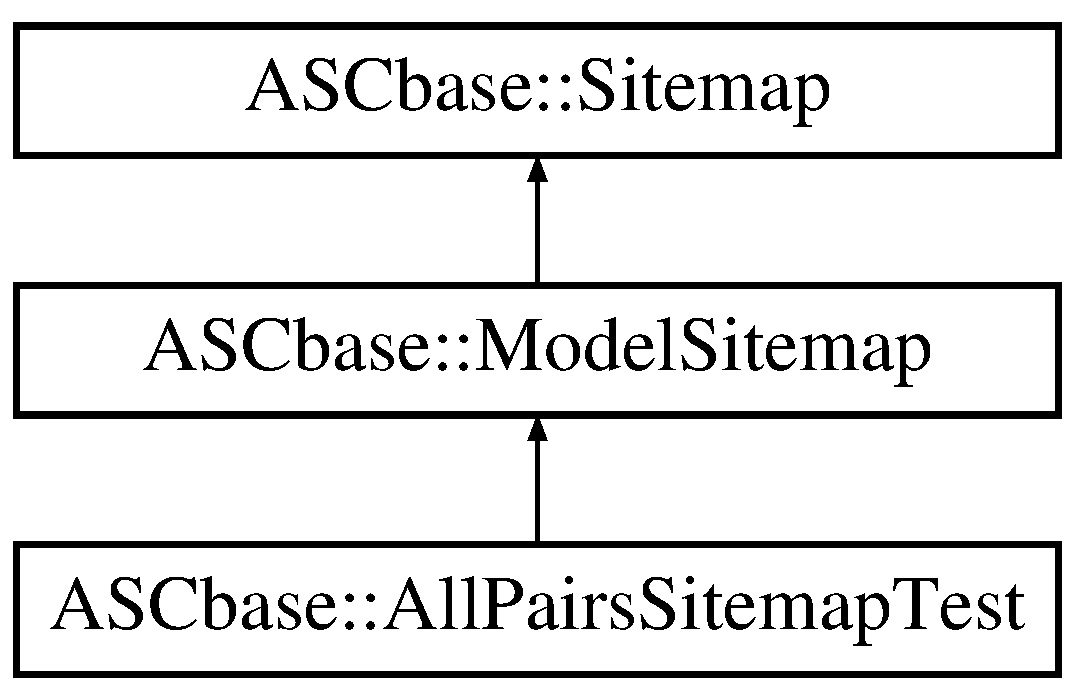
\includegraphics[height=3cm]{classASCbase_1_1ModelSitemap}
\end{center}
\end{figure}
\subsection*{Public Member Functions}
\begin{CompactItemize}
\item 
\textbf{Model\-Sitemap} (const std::string path, const std::string struct\_\-id, const \bf{Base\-Parameters} \&args, const my\_\-float\_\-t max\_\-corr\_\-surf\_\-pt\_\-dist, const bool normalize=true, const bool load\_\-hbond\_\-surfaces=false, const bool hydrophobic\_\-query=false)\label{classASCbase_1_1ModelSitemap_867ff44d757f97682de8c12b548058f4}

\item 
virtual bool \bf{get\_\-bucket\_\-iters} (const uint c, const my\_\-float\_\-t perimeter, const my\_\-float\_\-t max\_\-len, const my\_\-float\_\-t min\_\-len, bucket\_\-vci $\ast$bucket\_\-begin, bucket\_\-vci $\ast$bucket\_\-end)
\begin{CompactList}\small\item\em Given c,p,l,s get the iterators for the corresponding bucket. \item\end{CompactList}\item 
bool \textbf{report\_\-table\_\-stats} (std::ostream \&out)\label{classASCbase_1_1ModelSitemap_c9b820c6a0aac00bed61c1767a18bd40}

\item 
void \textbf{init\_\-positions\_\-octrees} (const my\_\-float\_\-t max\_\-dist, const my\_\-float\_\-t min\_\-side\_\-len, const uint max\_\-numel)\label{classASCbase_1_1ModelSitemap_c311885477fa9cb1e5ce25b1453cbde7}

\item 
void \textbf{transform} (const my\_\-float\_\-t $\ast$R, const my\_\-float\_\-t $\ast$T, const bool transform\_\-mesh=true, const bool transform\_\-hbond\_\-surfaces=true)\label{classASCbase_1_1ModelSitemap_2dccb51b62022b4e1d71ec357560f63b}

\item 
void \textbf{inverse\_\-transform} (const my\_\-float\_\-t $\ast$R, const my\_\-float\_\-t $\ast$T, const bool transform\_\-mesh=true, const bool transform\_\-hbond\_\-surfaces=true)\label{classASCbase_1_1ModelSitemap_962f9d9c2cd80c7266aa6adda57d0717}

\item 
void \textbf{revert} (const bool transform\_\-mesh=true, const bool transform\_\-hbond\_\-surfaces=true)\label{classASCbase_1_1ModelSitemap_ee7e2c3271b9e278ce926db772cb71ad}

\item 
void \bf{get\_\-current\_\-inverse\_\-3D\_\-transform} (Quaternion $\ast$Q, my\_\-float\_\-t $\ast$T) const 
\item 
const Model\-Hbond\-Surfaces $\ast$ \textbf{model\_\-hbond\_\-surfaces} () const \label{classASCbase_1_1ModelSitemap_c98f29ad6b6476713cbafbbc54fc6b6f}

\item 
const geometry::Transformable\-Trimesh \& \bf{binding\_\-site\_\-mesh\_\-handle} () const \label{classASCbase_1_1ModelSitemap_e7a43b0f03d4dd823c0ede8d4cc29d46}

\begin{CompactList}\small\item\em A constant reference to the binding site mesh surface. \item\end{CompactList}\item 
geometry::Transformable\-Trimesh \& \bf{mutable\_\-binding\_\-site\_\-mesh\_\-handle} ()
\begin{CompactList}\small\item\em A reference to the binding site mesh surface (not constant). \item\end{CompactList}\item 
Model\-Hbond\-Surfaces $\ast$ \textbf{mutable\_\-model\_\-hbond\_\-surfaces} ()\label{classASCbase_1_1ModelSitemap_60d3b8ec568b428b847592c596d24d8f}

\item 
bool \textbf{write\_\-msms\_\-caps} (std::string \&ofname\_\-pref)\label{classASCbase_1_1ModelSitemap_8d878cece922995a4ca9309635814c75}

\item 
void \bf{compute\_\-max\_\-feature\_\-vals} (std::vector$<$ my\_\-float\_\-t $>$ $\ast$max\_\-feat\_\-vals, const my\_\-float\_\-t max\_\-corr\_\-surf\_\-pt\_\-dist) const 
\item 
const std::vector$<$ my\_\-float\_\-t $>$ \& \bf{get\_\-max\_\-feature\_\-vals} () const \label{classASCbase_1_1ModelSitemap_cf9b0b90ec3550aa567f535cde6fe5e5}

\begin{CompactList}\small\item\em Get a const ref to the vector holding the max feature values. \item\end{CompactList}\end{CompactItemize}
\subsection*{Static Public Attributes}
\begin{CompactItemize}
\item 
static const int \bf{pmax} = static\_\-cast$<$int$>$(ceil(BUCKETS\_\-PER\_\-A\_\-PERIMETER $\ast$ (MAX\_\-PERIMETER - MIN\_\-PERIMETER)))\label{classASCbase_1_1ModelSitemap_a5634a6027959b45a3098bee1283166f}

\begin{CompactList}\small\item\em Maximum number of buckets for the perimeter. \item\end{CompactList}\item 
static const int \bf{lmax} = static\_\-cast$<$int$>$(ceil(BUCKETS\_\-PER\_\-A\_\-LENGTH $\ast$ (MAX\_\-LONGEST\_\-SIDE - MIN\_\-LONGEST\_\-SIDE)))\label{classASCbase_1_1ModelSitemap_53d6aa7980a77592a0c27cd6fea4965f}

\begin{CompactList}\small\item\em Maximum number of buckets for the longest side. \item\end{CompactList}\item 
static const int \bf{smax} = static\_\-cast$<$int$>$(ceil(BUCKETS\_\-PER\_\-A\_\-LENGTH $\ast$ (MAX\_\-SHORTEST\_\-SIDE - MIN\_\-SHORTEST\_\-SIDE)))\label{classASCbase_1_1ModelSitemap_410c2a8f22da9fddc77937af1a2cb736}

\begin{CompactList}\small\item\em Maximum number of buckets for the shortest side. \item\end{CompactList}\item 
static const my\_\-float\_\-t \textbf{MIN\_\-PERIMETER} = 9.0\label{classASCbase_1_1ModelSitemap_b14c04394ceb79fd8365f3ce0162ccce}

\item 
static const my\_\-float\_\-t \textbf{MAX\_\-PERIMETER} = 13.0\label{classASCbase_1_1ModelSitemap_3fe698b97d315dfea97646abc9d24868}

\item 
static const my\_\-float\_\-t \textbf{MIN\_\-LONGEST\_\-SIDE} = 3.5\label{classASCbase_1_1ModelSitemap_9362b8b3cc240e2b02f1ea446d3c1dbf}

\item 
static const my\_\-float\_\-t \textbf{MAX\_\-LONGEST\_\-SIDE} = 4.5\label{classASCbase_1_1ModelSitemap_92930656d9837c10aa47accb1540789d}

\item 
static const my\_\-float\_\-t \textbf{MIN\_\-SHORTEST\_\-SIDE} = 1.8\label{classASCbase_1_1ModelSitemap_7bbfb51cecd90e185e908181a32e8434}

\item 
static const my\_\-float\_\-t \textbf{MAX\_\-SHORTEST\_\-SIDE} = 3.5\label{classASCbase_1_1ModelSitemap_668d885229fbb9e4f5c551bdc58e6138}

\item 
static const uint \textbf{BUCKETS\_\-PER\_\-A\_\-PERIMETER} = 2\label{classASCbase_1_1ModelSitemap_07f175688297c1a86d5e63f9498bf170}

\item 
static const uint \textbf{BUCKETS\_\-PER\_\-A\_\-LENGTH} = 4\label{classASCbase_1_1ModelSitemap_1c0326a773ef0fb7b1641888938f028b}

\item 
static const uint \textbf{NUMBER\_\-OF\_\-TYPE\_\-HASH\_\-CLASSES} = 10\label{classASCbase_1_1ModelSitemap_3904d4119e0cf9545db7500712f00e90}

\item 
static const std::string \bf{\_\-fname} = \char`\"{}Model\-Sitemap.C\char`\"{}\label{classASCbase_1_1ModelSitemap_7daed5db065d1e266a4e28ef06de4b7c}

\begin{CompactList}\small\item\em Source file name. \item\end{CompactList}\end{CompactItemize}
\subsection*{Private Member Functions}
\begin{CompactItemize}
\item 
void \bf{clear} ()\label{classASCbase_1_1ModelSitemap_f67e8f1d3ea2c3611e8dce20551bd7b4}

\begin{CompactList}\small\item\em Frees any allocated objects \& calls \doxyref{init()}{p.}{classASCbase_1_1ModelSitemap_1dcf42cb09e1769e6b5ca6a97cd91f33} afterwards. \item\end{CompactList}\item 
void \bf{init} ()
\item 
void \textbf{create\_\-index\_\-table} ()\label{classASCbase_1_1ModelSitemap_085049cd46d725e5cb50a36662d4b261}

\item 
void \textbf{compute\_\-combinations} (std::vector$<$ uint $>$ $\ast$arr\_\-p, int index, int length)\label{classASCbase_1_1ModelSitemap_f4420b2eeaebf9c570fdb2794a9da743}

\end{CompactItemize}
\subsection*{Private Attributes}
\begin{CompactItemize}
\item 
std::list$<$ \bf{triangle\_\-t} $>$ \textbf{triangles}\label{classASCbase_1_1ModelSitemap_d0e5aa42b68b421aaf34a12b86e17ae3}

\item 
index\_\-table\_\-t \textbf{index\_\-table}\label{classASCbase_1_1ModelSitemap_849c23d851fac3808d6149a8159c26d0}

\item 
interact\_\-pts\_\-vci \bf{A\_\-pts\_\-begin}\label{classASCbase_1_1ModelSitemap_b6c180529920ca587be9eceb162a19b1}

\begin{CompactList}\small\item\em Iterator to the first split point (orig positions). \item\end{CompactList}\item 
Model\-Hbond\-Surfaces $\ast$ \textbf{A\_\-model\_\-hbond\_\-surfaces}\label{classASCbase_1_1ModelSitemap_48605cd2ecf6ceb6fc56e27d738abdfa}

\item 
geometry::Transformable\-Trimesh $\ast$ \textbf{A\_\-binding\_\-site\_\-mesh}\label{classASCbase_1_1ModelSitemap_065aa316a78f8ce7f1b846e2b83c9fba}

\item 
std::vector$<$ my\_\-float\_\-t $>$ \textbf{A\_\-max\_\-feature\_\-vals}\label{classASCbase_1_1ModelSitemap_ef737af4095b44e2273910fd884d1e05}

\end{CompactItemize}


\subsection{Detailed Description}
Create and provide an interface to the index table for the model (query) sitemap 



\subsection{Member Function Documentation}
\index{ASCbase::ModelSitemap@{ASCbase::Model\-Sitemap}!compute_max_feature_vals@{compute\_\-max\_\-feature\_\-vals}}
\index{compute_max_feature_vals@{compute\_\-max\_\-feature\_\-vals}!ASCbase::ModelSitemap@{ASCbase::Model\-Sitemap}}
\subsubsection{\setlength{\rightskip}{0pt plus 5cm}void Model\-Sitemap::compute\_\-max\_\-feature\_\-vals (std::vector$<$ my\_\-float\_\-t $>$ $\ast$ {\em max\_\-feat\_\-vals}, const my\_\-float\_\-t {\em max\_\-corr\_\-surf\_\-pt\_\-dist}) const}\label{classASCbase_1_1ModelSitemap_7327ff0f1e5e36866aeed2e32dd2dabb}


Compute the maximum value for each feature and store in the given vector \index{ASCbase::ModelSitemap@{ASCbase::Model\-Sitemap}!get_bucket_iters@{get\_\-bucket\_\-iters}}
\index{get_bucket_iters@{get\_\-bucket\_\-iters}!ASCbase::ModelSitemap@{ASCbase::Model\-Sitemap}}
\subsubsection{\setlength{\rightskip}{0pt plus 5cm}bool Model\-Sitemap::get\_\-bucket\_\-iters (const uint {\em c}, const my\_\-float\_\-t {\em perimeter}, const my\_\-float\_\-t {\em max\_\-len}, const my\_\-float\_\-t {\em min\_\-len}, bucket\_\-vci $\ast$ {\em bucket\_\-begin}, bucket\_\-vci $\ast$ {\em bucket\_\-end})\hspace{0.3cm}{\tt  [virtual]}}\label{classASCbase_1_1ModelSitemap_c80869d4e5b99f09d776f48c157fd52c}


Given c,p,l,s get the iterators for the corresponding bucket. 

Given the indexes into the index table, set the pointers to the begin and end of the bucket.

\begin{Desc}
\item[Parameters:]
\begin{description}
\item[{\em c}]hash\_\-class index \item[{\em p}]perimeter level index \item[{\em l}]longest edge length index \item[{\em s}]shortest edge length index \item[{\em bucket\_\-begin}]Pointer to the beginning of the bucket \item[{\em bucket\_\-end}]Pointer to the end of the bucket \end{description}
\end{Desc}
\begin{Desc}
\item[Returns:]true if bucket is nonempty \end{Desc}


Reimplemented in \bf{ASCbase::All\-Pairs\-Sitemap\-Test} \doxyref{p.}{classASCbase_1_1AllPairsSitemapTest_662913221bdc0a3063def4d40dd0d6f5}.\index{ASCbase::ModelSitemap@{ASCbase::Model\-Sitemap}!get_current_inverse_3D_transform@{get\_\-current\_\-inverse\_\-3D\_\-transform}}
\index{get_current_inverse_3D_transform@{get\_\-current\_\-inverse\_\-3D\_\-transform}!ASCbase::ModelSitemap@{ASCbase::Model\-Sitemap}}
\subsubsection{\setlength{\rightskip}{0pt plus 5cm}void ASCbase::Model\-Sitemap::get\_\-current\_\-inverse\_\-3D\_\-transform (Quaternion $\ast$ {\em Q}, my\_\-float\_\-t $\ast$ {\em T}) const\hspace{0.3cm}{\tt  [inline]}}\label{classASCbase_1_1ModelSitemap_1081951b9ad9b1b6f26578a3c1d2a8f5}


Get transform to move current hbond fit points to original position of the hbond fit points \index{ASCbase::ModelSitemap@{ASCbase::Model\-Sitemap}!init@{init}}
\index{init@{init}!ASCbase::ModelSitemap@{ASCbase::Model\-Sitemap}}
\subsubsection{\setlength{\rightskip}{0pt plus 5cm}void Model\-Sitemap::init ()\hspace{0.3cm}{\tt  [private]}}\label{classASCbase_1_1ModelSitemap_1dcf42cb09e1769e6b5ca6a97cd91f33}


Initializes pointers to 0 and other variables to 0 or another useful value 

Reimplemented from \bf{ASCbase::Sitemap} \doxyref{p.}{classASCbase_1_1Sitemap_2c579b022413645a8ecbdc4317117563}.\index{ASCbase::ModelSitemap@{ASCbase::Model\-Sitemap}!mutable_binding_site_mesh_handle@{mutable\_\-binding\_\-site\_\-mesh\_\-handle}}
\index{mutable_binding_site_mesh_handle@{mutable\_\-binding\_\-site\_\-mesh\_\-handle}!ASCbase::ModelSitemap@{ASCbase::Model\-Sitemap}}
\subsubsection{\setlength{\rightskip}{0pt plus 5cm}geometry::Transformable\-Trimesh\& ASCbase::Model\-Sitemap::mutable\_\-binding\_\-site\_\-mesh\_\-handle ()\hspace{0.3cm}{\tt  [inline]}}\label{classASCbase_1_1ModelSitemap_0f9ee82ed7959390abd7d38ac7d73a50}


A reference to the binding site mesh surface (not constant). 

Use this function with care -- at the present it should only be used when initializing a \doxyref{Surf\-Deps\-Joints}{p.}{classASCbase_1_1SurfDepsJoints} instance 

The documentation for this class was generated from the following files:\begin{CompactItemize}
\item 
Model\-Sitemap.H\item 
Model\-Sitemap.C\end{CompactItemize}

\section{ASCbase::Model\-Site\-RMSD Class Reference}
\label{classASCbase_1_1ModelSiteRMSD}\index{ASCbase::ModelSiteRMSD@{ASCbase::ModelSiteRMSD}}
Weight interaction NN interaction pair sums.  


{\tt \#include $<$Model\-Site\-RMSD.H$>$}

Inheritance diagram for ASCbase::Model\-Site\-RMSD::\begin{figure}[H]
\begin{center}
\leavevmode
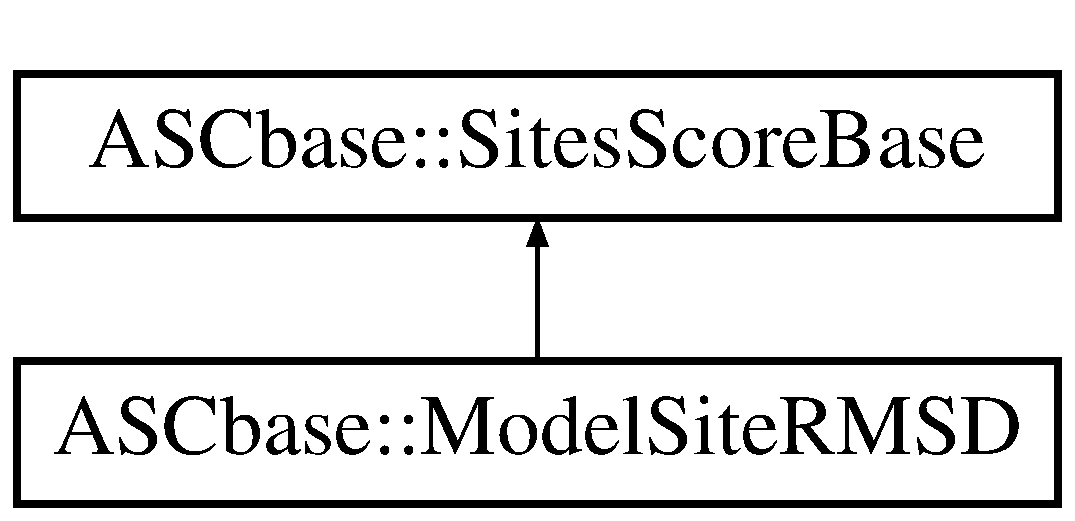
\includegraphics[height=2cm]{classASCbase_1_1ModelSiteRMSD}
\end{center}
\end{figure}
\subsection*{Public Types}
\begin{CompactItemize}
\item 
typedef std::less$<$ my\_\-float\_\-t $>$ \textbf{score\_\-cmp}\label{classASCbase_1_1ModelSiteRMSD_d7ff9231014ceb73af2c770d6647bf8f}

\end{CompactItemize}
\subsection*{Public Member Functions}
\begin{CompactItemize}
\item 
\bf{Model\-Site\-RMSD} ()\label{classASCbase_1_1ModelSiteRMSD_e6a786160b83da059ee9d9be896dd33e}

\begin{CompactList}\small\item\em Default constructor for site map point scoring of (aligned) sitemaps. \item\end{CompactList}\item 
virtual \bf{$\sim$Model\-Site\-RMSD} ()\label{classASCbase_1_1ModelSiteRMSD_68b9be473953d60d4f232ad789870df0}

\begin{CompactList}\small\item\em basic destruction \item\end{CompactList}\item 
my\_\-float\_\-t \bf{score} (const \bf{Model\-Sitemap} \&model, const \bf{Dbase\-Sitemap} \&dbase, \bf{rigid\_\-align\_\-t} $\ast$scores)
\item 
bool \bf{uses\_\-surface\_\-mesh} ()
\item 
bool \bf{uses\_\-hbond\_\-surfaces} ()
\end{CompactItemize}
\subsection*{Static Private Attributes}
\begin{CompactItemize}
\item 
static const std::string \bf{A\_\-fname}\label{classASCbase_1_1ModelSiteRMSD_095f57ffabd335008777bdccd789b6d7}

\begin{CompactList}\small\item\em Source file name. \item\end{CompactList}\end{CompactItemize}


\subsection{Detailed Description}
Weight interaction NN interaction pair sums. 



\subsection{Member Function Documentation}
\index{ASCbase::ModelSiteRMSD@{ASCbase::Model\-Site\-RMSD}!score@{score}}
\index{score@{score}!ASCbase::ModelSiteRMSD@{ASCbase::Model\-Site\-RMSD}}
\subsubsection{\setlength{\rightskip}{0pt plus 5cm}my\_\-float\_\-t ASCbase::Model\-Site\-RMSD::score (const \bf{Model\-Sitemap} \& {\em model}, const \bf{Dbase\-Sitemap} \& {\em dbase}, \bf{rigid\_\-align\_\-t} $\ast$ {\em scores})\hspace{0.3cm}{\tt  [inline, virtual]}}\label{classASCbase_1_1ModelSiteRMSD_3eb593c527ae195f94705cbc6b3ff335}


\begin{Desc}
\item[Parameters:]
\begin{description}
\item[{\em model}]Const ref to the model site \item[{\em dbase}]Const ref to the sitemap aligned to the model sitemap \item[{\em scores}]iterator to the score data class \end{description}
\end{Desc}
\begin{Desc}
\item[Returns:]The score of the alignment \end{Desc}


Implements \bf{ASCbase::Sites\-Score\-Base} \doxyref{p.}{classASCbase_1_1SitesScoreBase_651f05f08e15b7ea8f7fa7c41973499e}.\index{ASCbase::ModelSiteRMSD@{ASCbase::Model\-Site\-RMSD}!uses_hbond_surfaces@{uses\_\-hbond\_\-surfaces}}
\index{uses_hbond_surfaces@{uses\_\-hbond\_\-surfaces}!ASCbase::ModelSiteRMSD@{ASCbase::Model\-Site\-RMSD}}
\subsubsection{\setlength{\rightskip}{0pt plus 5cm}bool ASCbase::Model\-Site\-RMSD::uses\_\-hbond\_\-surfaces ()\hspace{0.3cm}{\tt  [inline, virtual]}}\label{classASCbase_1_1ModelSiteRMSD_8eb481fde2008dc2d6e60a3a4679bb07}


Derived class should return false, unless the derived class is using the hydrogen bond surface caps 

Reimplemented from \bf{ASCbase::Sites\-Score\-Base} \doxyref{p.}{classASCbase_1_1SitesScoreBase_a7a5fcc3e24663874f8066c00089f3cf}.\index{ASCbase::ModelSiteRMSD@{ASCbase::Model\-Site\-RMSD}!uses_surface_mesh@{uses\_\-surface\_\-mesh}}
\index{uses_surface_mesh@{uses\_\-surface\_\-mesh}!ASCbase::ModelSiteRMSD@{ASCbase::Model\-Site\-RMSD}}
\subsubsection{\setlength{\rightskip}{0pt plus 5cm}bool ASCbase::Model\-Site\-RMSD::uses\_\-surface\_\-mesh ()\hspace{0.3cm}{\tt  [inline, virtual]}}\label{classASCbase_1_1ModelSiteRMSD_f0f87f1b1293e8c294d24922ba2458b3}


Derived class should return false, unless, the site's surface needs to be to be rotated and translated 

Reimplemented from \bf{ASCbase::Sites\-Score\-Base} \doxyref{p.}{classASCbase_1_1SitesScoreBase_ae4a2a1ae9113bcad0535593c210030f}.

The documentation for this class was generated from the following file:\begin{CompactItemize}
\item 
Model\-Site\-RMSD.H\end{CompactItemize}

\section{ASCbase::mol2\_\-bond\_\-t Struct Reference}
\label{structASCbase_1_1mol2__bond__t}\index{ASCbase::mol2_bond_t@{ASCbase::mol2\_\-bond\_\-t}}
$<$ Fields of a mol2 bond record  


{\tt \#include $<$mol2File.H$>$}

\subsection*{Public Attributes}
\begin{CompactItemize}
\item 
bond\_\-type \bf{type}\label{structASCbase_1_1mol2__bond__t_777a617664920a145b9140c075474cdb}

\begin{CompactList}\small\item\em Type of bond (single, double, etc.). \item\end{CompactList}\item 
int \bf{atom\_\-num1}\label{structASCbase_1_1mol2__bond__t_aec7cb5b3bf6df2d4366f5368df5aef1}

\begin{CompactList}\small\item\em First atom in the bond (as listed in the file). \item\end{CompactList}\item 
int \bf{atom\_\-num2}\label{structASCbase_1_1mol2__bond__t_27316559fbc429818786482aa159c1e1}

\begin{CompactList}\small\item\em Second atom in the bond (as listed in the file). \item\end{CompactList}\item 
std::string \bf{status\_\-bits}\label{structASCbase_1_1mol2__bond__t_435f1fb617a87b857af38482c60cfa4e}

\begin{CompactList}\small\item\em Everything else on the line after the 2 atoms. \item\end{CompactList}\end{CompactItemize}


\subsection{Detailed Description}
$<$ Fields of a mol2 bond record 



The documentation for this struct was generated from the following file:\begin{CompactItemize}
\item 
mol2File.H\end{CompactItemize}

\section{ASCbase::mol2File Class Reference}
\label{classASCbase_1_1mol2File}\index{ASCbase::mol2File@{ASCbase::mol2File}}
Read and write mol2 files and perform various operations.  


{\tt \#include $<$mol2File.H$>$}

Inheritance diagram for ASCbase::mol2File::\begin{figure}[H]
\begin{center}
\leavevmode
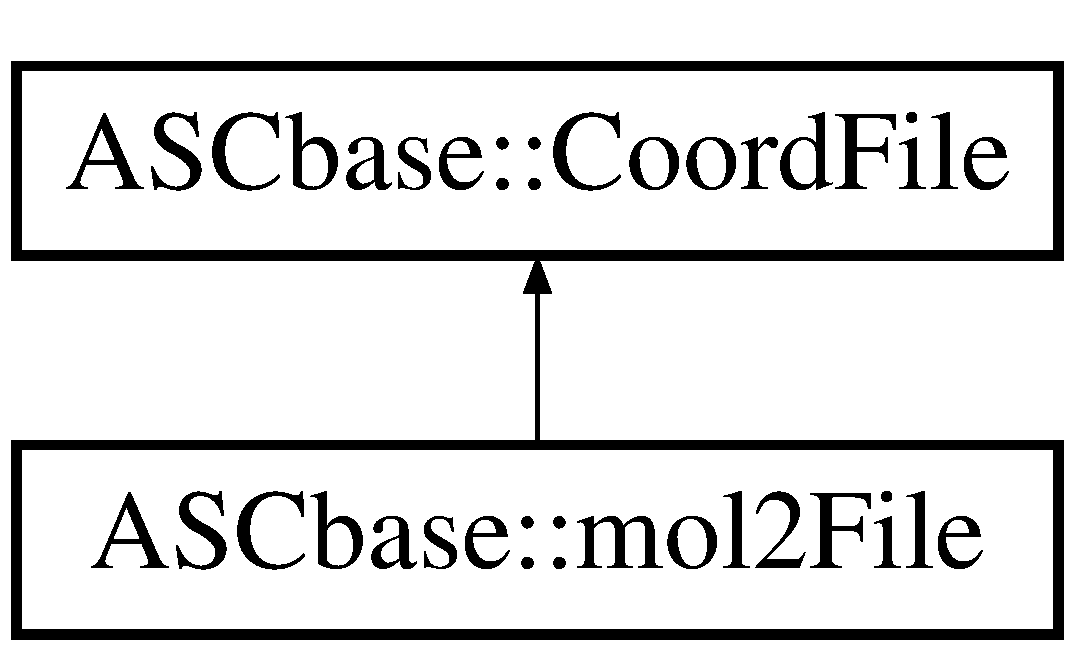
\includegraphics[height=2cm]{classASCbase_1_1mol2File}
\end{center}
\end{figure}
\subsection*{Public Member Functions}
\begin{CompactItemize}
\item 
\bf{mol2File} (const std::string filename, const verbose\_\-level\_\-t verbosity=VERBOSE\_\-SILENT)
\begin{CompactList}\small\item\em Constructor -- reads in the file and sets up the structure. \item\end{CompactList}\item 
\bf{mol2File} (const \bf{mol2File} \&src, const \bf{Bounding\-Volume} \&site\_\-vol, const \bf{Coord\-File} \&prot\_\-atoms, const uint min\_\-num\_\-atoms, const my\_\-float\_\-t $\ast$R, const my\_\-float\_\-t $\ast$T)
\begin{CompactList}\small\item\em Copy constructor -- fragments the ligand. \item\end{CompactList}\item 
\bf{$\sim$mol2File} ()\label{classASCbase_1_1mol2File_c3c8ecaa09091961a32c131c2e9199f3}

\begin{CompactList}\small\item\em Do nothin dstor. \item\end{CompactList}\item 
void \bf{report\_\-stats} (std::ostream \&out)
\begin{CompactList}\small\item\em Each derived class should support some routine to report on the file. \item\end{CompactList}\item 
void \bf{revert\_\-positions} ()\label{classASCbase_1_1mol2File_4df38db9db07af42b91db5fd0519d78a}

\begin{CompactList}\small\item\em Set the current positions to those read from file (original positions). \item\end{CompactList}\item 
bool \bf{write} (std::string ofname)
\begin{CompactList}\small\item\em Write the molecule(s) to the specified file. \item\end{CompactList}\item 
const uint \bf{num\_\-heavy\_\-atoms} ()\label{classASCbase_1_1mol2File_ac4b079f975345f69ad63b689f6bb3f5}

\begin{CompactList}\small\item\em Get the number of heavy atoms in the molecule(s). \item\end{CompactList}\item 
std::vector$<$ bool $>$::const\_\-iterator \bf{frag\_\-atoms\_\-flags\_\-beg} ()
\item 
std::vector$<$ bool $>$::const\_\-iterator \bf{frag\_\-atoms\_\-flags\_\-end} ()
\item 
const std::vector$<$ atom\_\-vci $>$ \& \bf{get\_\-nbrs} (const atom\_\-vci atom) const 
\item 
std::string \textbf{atom\_\-type\_\-to\_\-str} (const atom\_\-vci atom)\label{classASCbase_1_1mol2File_a835e7086af8dd4ea8e315b58666324d}

\item 
bool \textbf{calc\_\-charge\_\-sums} ()\label{classASCbase_1_1mol2File_cd1b6001933a4461f79c35d2ed482daa}

\end{CompactItemize}
\subsection*{Private Member Functions}
\begin{CompactItemize}
\item 
bool \bf{read\_\-data} (std::ifstream \&mol2\_\-file)
\item 
bool \bf{read\_\-molecule\_\-section} (std::ifstream \&mol2\_\-file, uint $\ast$num\_\-atoms\_\-out, uint $\ast$num\_\-bonds\_\-out)\label{classASCbase_1_1mol2File_89e45a813cec79c2e095a5bfd8a77f67}

\begin{CompactList}\small\item\em Read the first molecule section. \item\end{CompactList}\item 
bool \bf{read\_\-atom\_\-section} (std::ifstream \&mol2\_\-file, const uint num\_\-atoms)\label{classASCbase_1_1mol2File_01383b135389cc03960445865d57fe87}

\begin{CompactList}\small\item\em Read the first atom section after the first molecule section. \item\end{CompactList}\item 
bool \bf{read\_\-bond\_\-section} (std::ifstream \&mol2\_\-file, const uint num\_\-bonds)\label{classASCbase_1_1mol2File_aebc4bf5f53617b0e6014300bd40e608}

\begin{CompactList}\small\item\em Read the first bond section after the first atom section. \item\end{CompactList}\item 
bool \bf{look\_\-up\_\-atom\_\-by\_\-string} (const std::string atom\_\-str, \bf{atom\_\-t} $\ast$atom)\label{classASCbase_1_1mol2File_d8c08befaed6c64a8752e5f6f43b63f0}

\begin{CompactList}\small\item\em Given mol2 atom and orbital string, get internal info on atom. \item\end{CompactList}\item 
bool \bf{look\_\-up\_\-bond\_\-by\_\-string} (const std::string bond\_\-str, \bf{mol2\_\-bond\_\-t} $\ast$bond)\label{classASCbase_1_1mol2File_632bf1f1d3c95fd67ab1799753309a78}

\begin{CompactList}\small\item\em Given mol2 bond string, get internal bond type. \item\end{CompactList}\item 
void \bf{init\_\-atom\_\-table\_\-by\_\-string} ()\label{classASCbase_1_1mol2File_29239519d712966a47a89c6658952ade}

\begin{CompactList}\small\item\em Setup the map used to look up atom info based on mol2 atom and orbital. \item\end{CompactList}\item 
void \bf{init\_\-bond\_\-table\_\-by\_\-string} ()\label{classASCbase_1_1mol2File_2cf17eb0c5a571259113af56b98ef615}

\begin{CompactList}\small\item\em Setup the map to convert from mol2 bond string to internal bond type. \item\end{CompactList}\item 
void \bf{init\_\-bond\_\-types\_\-to\_\-str} ()\label{classASCbase_1_1mol2File_3bc5899510eadb43c23f2ab11393baa9}

\begin{CompactList}\small\item\em Setup the map to convert from interal bond type to mol2 bond string. \item\end{CompactList}\item 
void \bf{init\_\-atom\_\-types\_\-to\_\-str} ()
\item 
void \textbf{add\_\-bond} (const uint a1, const uint a2, const bond\_\-type type, const std::string status\_\-bits)\label{classASCbase_1_1mol2File_e16024d1b4aa6847320f9014ef056929}

\item 
bool \textbf{assign\_\-act\_\-types} ()\label{classASCbase_1_1mol2File_c82eec85dee77e4c25da6d769f7d4c0e}

\item 
void \textbf{generate\_\-nbrs\_\-vec} ()\label{classASCbase_1_1mol2File_cb742dce4a6b0b2ecc060efa71831672}

\end{CompactItemize}
\subsection*{Private Attributes}
\begin{CompactItemize}
\item 
std::string \textbf{A\_\-mol\_\-name}\label{classASCbase_1_1mol2File_4a239c4b6ef9219e5a6e1bcaf24abd6b}

\item 
std::string \textbf{A\_\-mol\_\-type}\label{classASCbase_1_1mol2File_0c181617cd1dfdba0349866cd0c50228}

\item 
std::string \textbf{A\_\-charge\_\-type}\label{classASCbase_1_1mol2File_26ec305f2afdc4dcc89b393583a1a3ff}

\item 
std::map$<$ std::string, const mol2\_\-atom\_\-info\_\-t $\ast$ $>$ \textbf{atoms\_\-by\_\-type\_\-str}\label{classASCbase_1_1mol2File_fe494476e111dd553575e619b05c152c}

\item 
std::map$<$ std::string, bond\_\-type $>$ \textbf{bonds\_\-by\_\-type\_\-str}\label{classASCbase_1_1mol2File_109be33ef75390bd6ecfd089047d089d}

\item 
std::map$<$ bond\_\-type, std::string $>$ \textbf{bond\_\-types\_\-to\_\-str}\label{classASCbase_1_1mol2File_272cffb8d8134d3479509dffd2d713c7}

\item 
std::map$<$ atom\_\-type, std::map$<$ orbit\_\-type, std::string $>$ $>$ \textbf{atom\_\-types\_\-to\_\-str}\label{classASCbase_1_1mol2File_e2f2b5510e400d2f8bffb5f4960a70f7}

\item 
std::vector$<$ std::string $>$ \textbf{rest\_\-of\_\-lines}\label{classASCbase_1_1mol2File_fac5b8259ea43796ddf98642432d513b}

\item 
mol2\_\-bond\_\-vec \bf{bonds}\label{classASCbase_1_1mol2File_1a674f42d6702f792adfa852a48f24eb}

\begin{CompactList}\small\item\em Rest of the atom lines. \item\end{CompactList}\item 
bool \textbf{atom\_\-ids\_\-are\_\-consecutive}\label{classASCbase_1_1mol2File_799f9c155bbe3f70a26fd8a2cfa2b3ab}

\item 
bool \bf{is\_\-frag\_\-file}\label{classASCbase_1_1mol2File_c3b92d4de315f32a750cf70bf3e776a5}

\begin{CompactList}\small\item\em True if the molecule is a fragment, else false. \item\end{CompactList}\item 
uint \textbf{a\_\-num\_\-heavy\_\-atoms}\label{classASCbase_1_1mol2File_4ed3d8244528aa77369514f27b4d417d}

\item 
std::vector$<$ bool $>$ \bf{frag\_\-atoms}\label{classASCbase_1_1mol2File_ce4ef757c3a959846fc802b6c9ac5cf7}

\begin{CompactList}\small\item\em Bool string of atoms present in fragment. \item\end{CompactList}\item 
std::vector$<$ std::vector$<$ atom\_\-vci $>$ $>$ \textbf{A\_\-nbrs\_\-vec}\label{classASCbase_1_1mol2File_5527c87e8143a7c1d88929a5059f21e5}

\end{CompactItemize}
\subsection*{Static Private Attributes}
\begin{CompactItemize}
\item 
static const my\_\-float\_\-t \textbf{ATOMS\_\-TOO\_\-FAR} = 4.5\label{classASCbase_1_1mol2File_64a9ac2baaaca25e2390a71920193994}

\item 
static const my\_\-float\_\-t \textbf{ATOMS\_\-TOO\_\-CLOSE} = 1.75\label{classASCbase_1_1mol2File_d4e8c046a3d397bb31c2e490bbde6827}

\item 
static const std::string \bf{\_\-fname} = \char`\"{}mol2File.C\char`\"{}\label{classASCbase_1_1mol2File_b7069d02b480b1de4486d2a9c5665fa1}

\begin{CompactList}\small\item\em Name of source file. \item\end{CompactList}\item 
static const my\_\-float\_\-t \textbf{MINIMAL\_\-CHARGE} = 0.5\label{classASCbase_1_1mol2File_f3f904ef0e8e6cd03c3eadb901a83534}

\end{CompactItemize}
\subsection*{Classes}
\begin{CompactItemize}
\item 
struct \bf{nbr\_\-bond\_\-type}
\begin{CompactList}\small\item\em Simple temporary type to store bond info in a vector. \item\end{CompactList}\end{CompactItemize}


\subsection{Detailed Description}
Read and write mol2 files and perform various operations. 

This class has 2 constructors. The first is to read the molecule(s) from a given file. The second constructor is a copy constructor and requires a protein and sitemap. This copy constructor discards all ligand atoms (in the copy) that are not within 2.0 (A) of any template point. These atoms are then checked to ensure that they do not significantly overlap with the protein. All of the ligand fragments are checked to ensure that they each have at least N connected heavy atoms. 



\subsection{Constructor \& Destructor Documentation}
\index{ASCbase::mol2File@{ASCbase::mol2File}!mol2File@{mol2File}}
\index{mol2File@{mol2File}!ASCbase::mol2File@{ASCbase::mol2File}}
\subsubsection{\setlength{\rightskip}{0pt plus 5cm}mol2File::mol2File (const std::string {\em filename}, const verbose\_\-level\_\-t {\em verbosity} = {\tt VERBOSE\_\-SILENT})}\label{classASCbase_1_1mol2File_9abfe2130ac705d98538e620541dbc28}


Constructor -- reads in the file and sets up the structure. 

\begin{Desc}
\item[Parameters:]
\begin{description}
\item[{\em filename}]Path of the mol2 file to read \end{description}
\end{Desc}
\index{ASCbase::mol2File@{ASCbase::mol2File}!mol2File@{mol2File}}
\index{mol2File@{mol2File}!ASCbase::mol2File@{ASCbase::mol2File}}
\subsubsection{\setlength{\rightskip}{0pt plus 5cm}mol2File::mol2File (const \bf{mol2File} \& {\em src}, const \bf{Bounding\-Volume} \& {\em site\_\-vol}, const \bf{Coord\-File} \& {\em prot\_\-atoms}, const uint {\em min\_\-num\_\-atoms}, const my\_\-float\_\-t $\ast$ {\em R}, const my\_\-float\_\-t $\ast$ {\em T})}\label{classASCbase_1_1mol2File_b890d66be2effc7b300ec625c87a014c}


Copy constructor -- fragments the ligand. 

\begin{Desc}
\item[Parameters:]
\begin{description}
\item[{\em src}]Reference to the full ligand to copy (search ligand) \item[{\em site\_\-vol}]Reference to the sitemap volume estimate \item[{\em prot\_\-atoms}]Reference to the query protein atoms \item[{\em min\_\-num\_\-atoms}]Minimum number of atoms in a ligand fragment \item[{\em R}]Rotation matrix to move ligand to the model ref. frame \item[{\em T}]Translation vector to move ligand to the model ref. frame \end{description}
\end{Desc}


\subsection{Member Function Documentation}
\index{ASCbase::mol2File@{ASCbase::mol2File}!frag_atoms_flags_beg@{frag\_\-atoms\_\-flags\_\-beg}}
\index{frag_atoms_flags_beg@{frag\_\-atoms\_\-flags\_\-beg}!ASCbase::mol2File@{ASCbase::mol2File}}
\subsubsection{\setlength{\rightskip}{0pt plus 5cm}std::vector$<$bool$>$::const\_\-iterator ASCbase::mol2File::frag\_\-atoms\_\-flags\_\-beg ()\hspace{0.3cm}{\tt  [inline]}}\label{classASCbase_1_1mol2File_27ca8161c7d240a8331a56912047dde0}


The vector referred to is of the same length as the number of atoms in the \char`\"{}original\char`\"{} ligand. The nth bool is true or false if the nth ligand atom is in a ligand fragment or is not in a ligand fragment respectively. \index{ASCbase::mol2File@{ASCbase::mol2File}!frag_atoms_flags_end@{frag\_\-atoms\_\-flags\_\-end}}
\index{frag_atoms_flags_end@{frag\_\-atoms\_\-flags\_\-end}!ASCbase::mol2File@{ASCbase::mol2File}}
\subsubsection{\setlength{\rightskip}{0pt plus 5cm}std::vector$<$bool$>$::const\_\-iterator ASCbase::mol2File::frag\_\-atoms\_\-flags\_\-end ()\hspace{0.3cm}{\tt  [inline]}}\label{classASCbase_1_1mol2File_a7662a32085ef964254c0f36285f9fb0}


Get a const iterator to the end of the boolean vector denoting which atoms of the full ligand were kept. \index{ASCbase::mol2File@{ASCbase::mol2File}!get_nbrs@{get\_\-nbrs}}
\index{get_nbrs@{get\_\-nbrs}!ASCbase::mol2File@{ASCbase::mol2File}}
\subsubsection{\setlength{\rightskip}{0pt plus 5cm}const std::vector$<$atom\_\-vci$>$\& ASCbase::mol2File::get\_\-nbrs (const atom\_\-vci {\em atom}) const\hspace{0.3cm}{\tt  [inline]}}\label{classASCbase_1_1mol2File_c112d4a0eaca36f7ffa1d635ab30a13f}


Get the neighbors of atom in this molecule. If someone wants to pass in an atom from another molecule, they will get rewarded with a const ref to an empty vector. \index{ASCbase::mol2File@{ASCbase::mol2File}!init_atom_types_to_str@{init\_\-atom\_\-types\_\-to\_\-str}}
\index{init_atom_types_to_str@{init\_\-atom\_\-types\_\-to\_\-str}!ASCbase::mol2File@{ASCbase::mol2File}}
\subsubsection{\setlength{\rightskip}{0pt plus 5cm}void mol2File::init\_\-atom\_\-types\_\-to\_\-str ()\hspace{0.3cm}{\tt  [private]}}\label{classASCbase_1_1mol2File_d0e57ec2d4706d8b22375a55aed5d71e}


Setup the map to convert from internal atom and orbital to mol2 atom string \index{ASCbase::mol2File@{ASCbase::mol2File}!read_data@{read\_\-data}}
\index{read_data@{read\_\-data}!ASCbase::mol2File@{ASCbase::mol2File}}
\subsubsection{\setlength{\rightskip}{0pt plus 5cm}bool mol2File::read\_\-data (std::ifstream \& {\em mol2\_\-file})\hspace{0.3cm}{\tt  [private, virtual]}}\label{classASCbase_1_1mol2File_da164682f58d1e4539666d13de03fb9a}


Top level read function -- read in the molecule(s) from the file passed to the constructor 

Implements \bf{ASCbase::Coord\-File} \doxyref{p.}{classASCbase_1_1CoordFile_1fdc54fd347269643062dee5418859a5}.\index{ASCbase::mol2File@{ASCbase::mol2File}!report_stats@{report\_\-stats}}
\index{report_stats@{report\_\-stats}!ASCbase::mol2File@{ASCbase::mol2File}}
\subsubsection{\setlength{\rightskip}{0pt plus 5cm}void mol2File::report\_\-stats (std::ostream \& {\em out})\hspace{0.3cm}{\tt  [virtual]}}\label{classASCbase_1_1mol2File_8621701ac72363cd41e08123cb4929af}


Each derived class should support some routine to report on the file. 

\begin{Desc}
\item[Parameters:]
\begin{description}
\item[{\em out}]Reference to the ostream to write the report \end{description}
\end{Desc}


Implements \bf{ASCbase::Coord\-File} \doxyref{p.}{classASCbase_1_1CoordFile_a2153c9f750dd76c3b533f9e03bd8f05}.\index{ASCbase::mol2File@{ASCbase::mol2File}!write@{write}}
\index{write@{write}!ASCbase::mol2File@{ASCbase::mol2File}}
\subsubsection{\setlength{\rightskip}{0pt plus 5cm}bool mol2File::write (std::string {\em ofname})\hspace{0.3cm}{\tt  [virtual]}}\label{classASCbase_1_1mol2File_050d5348e9f9a59de0949a66acab96de}


Write the molecule(s) to the specified file. 

\begin{Desc}
\item[Parameters:]
\begin{description}
\item[{\em ofname}]Name of the file to write molecule(s) \end{description}
\end{Desc}


Implements \bf{ASCbase::Coord\-File} \doxyref{p.}{classASCbase_1_1CoordFile_dca3f5f45c21f85215dc380e2152b613}.

The documentation for this class was generated from the following files:\begin{CompactItemize}
\item 
mol2File.H\item 
mol2File.C\end{CompactItemize}

\section{ASCbase::mol2File::nbr\_\-bond\_\-type Struct Reference}
\label{structASCbase_1_1mol2File_1_1nbr__bond__type}\index{ASCbase::mol2File::nbr_bond_type@{ASCbase::mol2File::nbr\_\-bond\_\-type}}
Simple temporary type to store bond info in a vector.  


\subsection*{Public Attributes}
\begin{CompactItemize}
\item 
atom\_\-vci \textbf{nbr}\label{structASCbase_1_1mol2File_1_1nbr__bond__type_a83f213d22c3c323abc1c4e0ea6dcd7c}

\item 
bond\_\-type \textbf{bond}\label{structASCbase_1_1mol2File_1_1nbr__bond__type_4ddb744e4eed89b40973c55f398addf1}

\end{CompactItemize}


\subsection{Detailed Description}
Simple temporary type to store bond info in a vector. 



The documentation for this struct was generated from the following file:\begin{CompactItemize}
\item 
mol2File.H\end{CompactItemize}

\section{ASCbase::my\_\-float\_\-array Class Reference}
\label{classASCbase_1_1my__float__array}\index{ASCbase::my_float_array@{ASCbase::my\_\-float\_\-array}}
Note no copy constructor so copying will result in pain.  


{\tt \#include $<$my\_\-float\_\-array.H$>$}

\subsection*{Public Member Functions}
\begin{CompactItemize}
\item 
\bf{my\_\-float\_\-array} (uint init\_\-num\_\-pts=10, uint stride\_\-in=3)\label{classASCbase_1_1my__float__array_d9b0cb450e669b9e4b7bdced7c36a466}

\begin{CompactList}\small\item\em Cstor to set up floating pt array. \item\end{CompactList}\item 
\bf{my\_\-float\_\-array} (const \bf{my\_\-float\_\-array} \&src)\label{classASCbase_1_1my__float__array_a6269a44c631f4fe16c92229f4f128e5}

\begin{CompactList}\small\item\em Copy in a reasonable manner. \item\end{CompactList}\item 
const \bf{my\_\-float\_\-array} \& \bf{operator=} (const \bf{my\_\-float\_\-array} \&src)
\item 
\bf{$\sim$my\_\-float\_\-array} ()\label{classASCbase_1_1my__float__array_604d58f23c22a431770fb11f97fc2a99}

\begin{CompactList}\small\item\em Dstor. \item\end{CompactList}\item 
uint \textbf{size} () const \label{classASCbase_1_1my__float__array_c15df63500d30ce66dee8a118b69821d}

\item 
uint \textbf{stride} () const \label{classASCbase_1_1my__float__array_ca02b23f8fd6e8a60a28e4cfae8a648e}

\item 
uint \textbf{reserved} () const \label{classASCbase_1_1my__float__array_ad39c32e4901faa77e113451f3292cd5}

\item 
my\_\-float\_\-t $\ast$ \textbf{begin} () const \label{classASCbase_1_1my__float__array_764b70c62326d6ed689ecc3fdce08c5a}

\item 
my\_\-float\_\-t $\ast$ \textbf{end} () const \label{classASCbase_1_1my__float__array_62e4444b755858beec023de8d9fceeef}

\item 
my\_\-float\_\-array\_\-push\_\-back\_\-return\_\-type \bf{push\_\-back} (const my\_\-float\_\-t $\ast$el)
\begin{CompactList}\small\item\em Push back an element of length \_\-stride onto the array. \item\end{CompactList}\item 
void \bf{transform3D} (const my\_\-float\_\-t $\ast$R, const my\_\-float\_\-t $\ast$T)
\begin{CompactList}\small\item\em Apply a rotation + translation current array. \item\end{CompactList}\item 
void \bf{inverse\_\-transform3D} (const my\_\-float\_\-t $\ast$R, const my\_\-float\_\-t $\ast$T)
\begin{CompactList}\small\item\em Apply a negative translation and inverse rotation. \item\end{CompactList}\item 
void \bf{revert} ()\label{classASCbase_1_1my__float__array_5612962a30bbc36661eab21d94a172a7}

\begin{CompactList}\small\item\em Reset the positions of the atoms to their original positions. \item\end{CompactList}\item 
void \bf{set\_\-current\_\-values\_\-as\_\-original} ()
\begin{CompactList}\small\item\em Set the current values as the original values. \item\end{CompactList}\item 
const bool \bf{centroid\_\-3D} (my\_\-float\_\-t $\ast$C) const \label{classASCbase_1_1my__float__array_c716853fd605ff6e32d4ede02cedb7b0}

\begin{CompactList}\small\item\em Get the centroid (assumes 3D points). \item\end{CompactList}\item 
void \bf{get\_\-current\_\-inverse\_\-3D\_\-transform} (Quaternion $\ast$Q, my\_\-float\_\-t $\ast$T) const 
\item 
my\_\-float\_\-t \bf{compute\_\-RMSD} () const 
\end{CompactItemize}
\subsection*{Private Member Functions}
\begin{CompactItemize}
\item 
void \textbf{init} ()\label{classASCbase_1_1my__float__array_cd4c500b6129b80a28b9aaf3c9253d2f}

\item 
void \bf{double\_\-reserve} ()\label{classASCbase_1_1my__float__array_70345204169e7017a18fb1c0de64336d}

\begin{CompactList}\small\item\em Double the array reserve. \item\end{CompactList}\item 
void \bf{update\_\-orig\_\-pts} ()\label{classASCbase_1_1my__float__array_2a888e41827034da0597d88b1e3470e7}

\begin{CompactList}\small\item\em Set the original array. \item\end{CompactList}\item 
void \bf{do\_\-copy} (const \bf{my\_\-float\_\-array} \&src)
\end{CompactItemize}
\subsection*{Private Attributes}
\begin{CompactItemize}
\item 
uint \textbf{\_\-stride}\label{classASCbase_1_1my__float__array_4af7ff17850cdafd9a355127d0f2cca0}

\item 
int \textbf{\_\-reserved}\label{classASCbase_1_1my__float__array_44dc5f56c5c8597129fcc91bf52bd093}

\item 
my\_\-float\_\-t $\ast$ \bf{orig}\label{classASCbase_1_1my__float__array_7bab1066585311c5b0e185761dcafd05}

\begin{CompactList}\small\item\em Beginning of points as added to this object. \item\end{CompactList}\item 
my\_\-float\_\-t $\ast$ \bf{orig\_\-end}\label{classASCbase_1_1my__float__array_22aefb5abe3a4e1ada9cacfb6b5464b3}

\begin{CompactList}\small\item\em End of points as added to this object. \item\end{CompactList}\item 
my\_\-float\_\-t $\ast$ \bf{curr}\label{classASCbase_1_1my__float__array_4dfcdb66fffd9a861988c5343f263ffd}

\begin{CompactList}\small\item\em Beginning of current points (after 0 or more transformations). \item\end{CompactList}\item 
my\_\-float\_\-t $\ast$ \bf{curr\_\-end}\label{classASCbase_1_1my__float__array_38577011f5ee6e411ef96f3a8b8143b2}

\begin{CompactList}\small\item\em End of current points (after 0 or more transformations). \item\end{CompactList}\item 
my\_\-float\_\-t $\ast$ \bf{scratch}\label{classASCbase_1_1my__float__array_4bab597976578f4d790991065b9b417e}

\begin{CompactList}\small\item\em Scratch space -- keep from frequently grabbing new mem. \item\end{CompactList}\end{CompactItemize}


\subsection{Detailed Description}
Note no copy constructor so copying will result in pain. 



\subsection{Member Function Documentation}
\index{ASCbase::my_float_array@{ASCbase::my\_\-float\_\-array}!compute_RMSD@{compute\_\-RMSD}}
\index{compute_RMSD@{compute\_\-RMSD}!ASCbase::my_float_array@{ASCbase::my\_\-float\_\-array}}
\subsubsection{\setlength{\rightskip}{0pt plus 5cm}my\_\-float\_\-t ASCbase::my\_\-float\_\-array::compute\_\-RMSD () const\hspace{0.3cm}{\tt  [inline]}}\label{classASCbase_1_1my__float__array_ea4337b692bde44840c4affc07cf7095}


Compute the root mean squared deviation (RMSD) between the current and orignial points \index{ASCbase::my_float_array@{ASCbase::my\_\-float\_\-array}!do_copy@{do\_\-copy}}
\index{do_copy@{do\_\-copy}!ASCbase::my_float_array@{ASCbase::my\_\-float\_\-array}}
\subsubsection{\setlength{\rightskip}{0pt plus 5cm}void my\_\-float\_\-array::do\_\-copy (const \bf{my\_\-float\_\-array} \& {\em src})\hspace{0.3cm}{\tt  [private]}}\label{classASCbase_1_1my__float__array_06718ce6dbd8d6904e31f34943499e09}


Copy routine -- everyone else is expected to handle any stale pointers \& updating \index{ASCbase::my_float_array@{ASCbase::my\_\-float\_\-array}!get_current_inverse_3D_transform@{get\_\-current\_\-inverse\_\-3D\_\-transform}}
\index{get_current_inverse_3D_transform@{get\_\-current\_\-inverse\_\-3D\_\-transform}!ASCbase::my_float_array@{ASCbase::my\_\-float\_\-array}}
\subsubsection{\setlength{\rightskip}{0pt plus 5cm}void ASCbase::my\_\-float\_\-array::get\_\-current\_\-inverse\_\-3D\_\-transform (Quaternion $\ast$ {\em Q}, my\_\-float\_\-t $\ast$ {\em T}) const\hspace{0.3cm}{\tt  [inline]}}\label{classASCbase_1_1my__float__array_f341a7e9e7bde491843bf95e61650eee}


Note: since a chain of transformations is in general difficult or even impossible to invert, this method is somewhat computationally expensive as it uses a least squares fit of all the points \index{ASCbase::my_float_array@{ASCbase::my\_\-float\_\-array}!inverse_transform3D@{inverse\_\-transform3D}}
\index{inverse_transform3D@{inverse\_\-transform3D}!ASCbase::my_float_array@{ASCbase::my\_\-float\_\-array}}
\subsubsection{\setlength{\rightskip}{0pt plus 5cm}void ASCbase::my\_\-float\_\-array::inverse\_\-transform3D (const my\_\-float\_\-t $\ast$ {\em R}, const my\_\-float\_\-t $\ast$ {\em T})\hspace{0.3cm}{\tt  [inline]}}\label{classASCbase_1_1my__float__array_36cecd78c077ff31ded38a0194b862f2}


Apply a negative translation and inverse rotation. 

Transform the positions by -T and then rotate by R$^\wedge$t \index{ASCbase::my_float_array@{ASCbase::my\_\-float\_\-array}!operator=@{operator=}}
\index{operator=@{operator=}!ASCbase::my_float_array@{ASCbase::my\_\-float\_\-array}}
\subsubsection{\setlength{\rightskip}{0pt plus 5cm}const \bf{my\_\-float\_\-array}\& ASCbase::my\_\-float\_\-array::operator= (const \bf{my\_\-float\_\-array} \& {\em src})\hspace{0.3cm}{\tt  [inline]}}\label{classASCbase_1_1my__float__array_cf2256fd42e02535450e38db5350b987}


Assignment operator -- other classes may need to take care of stale pointers \index{ASCbase::my_float_array@{ASCbase::my\_\-float\_\-array}!push_back@{push\_\-back}}
\index{push_back@{push\_\-back}!ASCbase::my_float_array@{ASCbase::my\_\-float\_\-array}}
\subsubsection{\setlength{\rightskip}{0pt plus 5cm}my\_\-float\_\-array\_\-push\_\-back\_\-return\_\-type ASCbase::my\_\-float\_\-array::push\_\-back (const my\_\-float\_\-t $\ast$ {\em el})\hspace{0.3cm}{\tt  [inline]}}\label{classASCbase_1_1my__float__array_d1cf330a07c7789f5ef224cc93374277}


Push back an element of length \_\-stride onto the array. 

If el does not have a length of at least \_\-stride, the operation is undefined.

Warning: do not use this function once the positions have been transformed or the results may be different than expected \index{ASCbase::my_float_array@{ASCbase::my\_\-float\_\-array}!set_current_values_as_original@{set\_\-current\_\-values\_\-as\_\-original}}
\index{set_current_values_as_original@{set\_\-current\_\-values\_\-as\_\-original}!ASCbase::my_float_array@{ASCbase::my\_\-float\_\-array}}
\subsubsection{\setlength{\rightskip}{0pt plus 5cm}void ASCbase::my\_\-float\_\-array::set\_\-current\_\-values\_\-as\_\-original ()\hspace{0.3cm}{\tt  [inline]}}\label{classASCbase_1_1my__float__array_a98bd8a8f5970ca4cd7523e15a0af9f8}


Set the current values as the original values. 

This functionality is useful when we want to read in a set of data points and apply some initial calculations and set the updated values as the original. In this way, we will revert to the initialized values and not the values when the array was first created. \index{ASCbase::my_float_array@{ASCbase::my\_\-float\_\-array}!transform3D@{transform3D}}
\index{transform3D@{transform3D}!ASCbase::my_float_array@{ASCbase::my\_\-float\_\-array}}
\subsubsection{\setlength{\rightskip}{0pt plus 5cm}void ASCbase::my\_\-float\_\-array::transform3D (const my\_\-float\_\-t $\ast$ {\em R}, const my\_\-float\_\-t $\ast$ {\em T})\hspace{0.3cm}{\tt  [inline]}}\label{classASCbase_1_1my__float__array_6539a83a54fe3c26d54f4bce4bfc7057}


Apply a rotation + translation current array. 

For now a BLAS interface is more of a dream than reality and the code used to implement BLAS routines would be at best the same speed as here (even though this might be dastardly slow comapred with ATLAS BLAS)

-- array version for(uint z = 0; z $<$ coords\_\-end - coords; z += 3) for(uint i = 0; i $<$ 3; ++i)\{ scratch[z + i] = T[i]; for(uint j = 0; j $<$ 3; ++j) scratch[z + i] += R[3$\ast$i + j] $\ast$ coords[z + j]; \} 

The documentation for this class was generated from the following files:\begin{CompactItemize}
\item 
my\_\-float\_\-array.H\item 
my\_\-float\_\-array.C\end{CompactItemize}

\section{ASCbase::No\-Tier1Score Class Reference}
\label{classASCbase_1_1NoTier1Score}\index{ASCbase::NoTier1Score@{ASCbase::NoTier1Score}}
A do nothing score -- used to check the value of the parameter.  


{\tt \#include $<$No\-Tier1Score.H$>$}

Inheritance diagram for ASCbase::No\-Tier1Score::\begin{figure}[H]
\begin{center}
\leavevmode
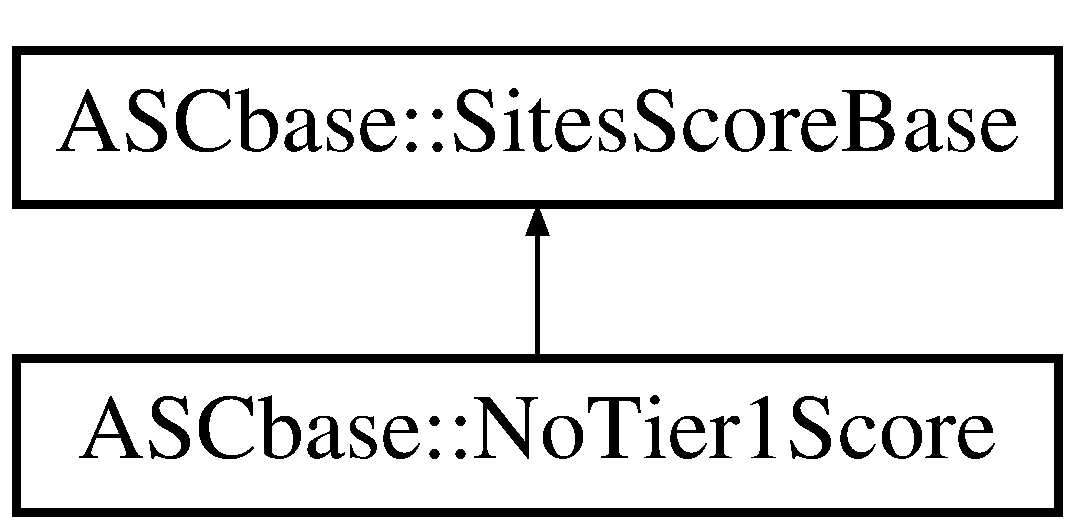
\includegraphics[height=2cm]{classASCbase_1_1NoTier1Score}
\end{center}
\end{figure}
\subsection*{Public Types}
\begin{CompactItemize}
\item 
typedef std::less$<$ my\_\-float\_\-t $>$ \textbf{score\_\-cmp}\label{classASCbase_1_1NoTier1Score_42fa102530c259b1e7d37210a572f498}

\end{CompactItemize}
\subsection*{Public Member Functions}
\begin{CompactItemize}
\item 
\bf{No\-Tier1Score} ()\label{classASCbase_1_1NoTier1Score_034e46ee6706ad30c721f2eccfd77224}

\begin{CompactList}\small\item\em Default constructor for site map point scoring of (aligned) sitemaps. \item\end{CompactList}\item 
\bf{$\sim$No\-Tier1Score} ()\label{classASCbase_1_1NoTier1Score_779535c36aa6de96071a94eb44c52068}

\begin{CompactList}\small\item\em basic destruction \item\end{CompactList}\item 
my\_\-float\_\-t \bf{score} (const \bf{Model\-Sitemap} \&model, const \bf{Dbase\-Sitemap} \&dbase, \bf{rigid\_\-align\_\-t} $\ast$scores)
\begin{CompactList}\small\item\em Returns my\_\-float\_\-max. \item\end{CompactList}\item 
bool \bf{uses\_\-surface\_\-mesh} ()
\item 
bool \bf{uses\_\-hbond\_\-surfaces} ()
\item 
const bool \bf{score\_\-is\_\-noop} () const \label{classASCbase_1_1NoTier1Score_63778c92095132cf82e34d7d5d62f7f8}

\begin{CompactList}\small\item\em This class's \doxyref{score()}{p.}{classASCbase_1_1NoTier1Score_1d4f4670c8831e655105788395100367} function score is a no op!! \item\end{CompactList}\end{CompactItemize}


\subsection{Detailed Description}
A do nothing score -- used to check the value of the parameter. 

Used to fill in the first C++ template parameter if we have only 1 tiered scoring. This is bogus, but it is currently the best I could think of in this short amoutn of time and still work well with the logic of fine tuning and not copy the vector of alignments 



\subsection{Member Function Documentation}
\index{ASCbase::NoTier1Score@{ASCbase::No\-Tier1Score}!score@{score}}
\index{score@{score}!ASCbase::NoTier1Score@{ASCbase::No\-Tier1Score}}
\subsubsection{\setlength{\rightskip}{0pt plus 5cm}my\_\-float\_\-t ASCbase::No\-Tier1Score::score (const \bf{Model\-Sitemap} \& {\em model}, const \bf{Dbase\-Sitemap} \& {\em dbase}, \bf{rigid\_\-align\_\-t} $\ast$ {\em scores})\hspace{0.3cm}{\tt  [inline, virtual]}}\label{classASCbase_1_1NoTier1Score_1d4f4670c8831e655105788395100367}


Returns my\_\-float\_\-max. 

\begin{Desc}
\item[Parameters:]
\begin{description}
\item[{\em model}]Const ref to the model site \item[{\em dbase}]Const ref to the sitemap aligned to the model sitemap \item[{\em scores}]iterator to the score data class \end{description}
\end{Desc}
\begin{Desc}
\item[Returns:]my\_\-float\_\-max \end{Desc}


Implements \bf{ASCbase::Sites\-Score\-Base} \doxyref{p.}{classASCbase_1_1SitesScoreBase_651f05f08e15b7ea8f7fa7c41973499e}.\index{ASCbase::NoTier1Score@{ASCbase::No\-Tier1Score}!uses_hbond_surfaces@{uses\_\-hbond\_\-surfaces}}
\index{uses_hbond_surfaces@{uses\_\-hbond\_\-surfaces}!ASCbase::NoTier1Score@{ASCbase::No\-Tier1Score}}
\subsubsection{\setlength{\rightskip}{0pt plus 5cm}bool ASCbase::No\-Tier1Score::uses\_\-hbond\_\-surfaces ()\hspace{0.3cm}{\tt  [inline, virtual]}}\label{classASCbase_1_1NoTier1Score_173cc857bbcd62849e9462cfa8c78a4b}


Derived class should return false, unless the derived class is using the hydrogen bond surface caps 

Reimplemented from \bf{ASCbase::Sites\-Score\-Base} \doxyref{p.}{classASCbase_1_1SitesScoreBase_a7a5fcc3e24663874f8066c00089f3cf}.\index{ASCbase::NoTier1Score@{ASCbase::No\-Tier1Score}!uses_surface_mesh@{uses\_\-surface\_\-mesh}}
\index{uses_surface_mesh@{uses\_\-surface\_\-mesh}!ASCbase::NoTier1Score@{ASCbase::No\-Tier1Score}}
\subsubsection{\setlength{\rightskip}{0pt plus 5cm}bool ASCbase::No\-Tier1Score::uses\_\-surface\_\-mesh ()\hspace{0.3cm}{\tt  [inline, virtual]}}\label{classASCbase_1_1NoTier1Score_39452ebad1db68af8cc2e3a4cb08953e}


Derived class should return false, unless, the site's surface needs to be to be rotated and translated 

Reimplemented from \bf{ASCbase::Sites\-Score\-Base} \doxyref{p.}{classASCbase_1_1SitesScoreBase_ae4a2a1ae9113bcad0535593c210030f}.

The documentation for this class was generated from the following file:\begin{CompactItemize}
\item 
No\-Tier1Score.H\end{CompactItemize}

\section{Octree$<$ \_\-Tp, \_\-Sequence $>$ Class Template Reference}
\label{classOctree}\index{Octree@{Octree}}
Simple \doxyref{Octree}{p.}{classOctree} for any datatype with an associated 3D position.  


{\tt \#include $<$Octree.H$>$}

\subsection*{Public Types}
\begin{CompactItemize}
\item 
typedef \_\-Sequence::value\_\-type \textbf{value\_\-type}\label{classOctree_8fb22bc26937ebd3f689f6cf2157d169}

\item 
typedef \_\-Sequence::const\_\-reference \textbf{const\_\-reference}\label{classOctree_4fd5790c52670b76c337bd9f08f294af}

\item 
typedef \_\-Sequence::const\_\-iterator \textbf{const\_\-iterator}\label{classOctree_28b30f494bae31705aeafb835c84daa8}

\item 
typedef \_\-Sequence \textbf{container\_\-type}\label{classOctree_07f30dd5b14c3ed60e709102145ca657}

\end{CompactItemize}
\subsection*{Public Member Functions}
\begin{CompactItemize}
\item 
\textbf{Octree} (const my\_\-float\_\-t min\_\-side\_\-len, const uint max\_\-numel=10)\label{classOctree_7a2590d8a632a07c764f4ce12b5387b3}

\item 
void \bf{build} (const my\_\-float\_\-t $\ast$positions\_\-begin, const my\_\-float\_\-t $\ast$postions\_\-end, const my\_\-float\_\-t $\ast$centroid, const my\_\-float\_\-t root\_\-side\_\-len, const container\_\-type \&data)
\item 
void \textbf{subdivide} (octree\_\-data\_\-t$<$ const\_\-iterator $>$ $\ast$cnode, const std::vector$<$ uint $>$ \&idz, const my\_\-float\_\-t $\ast$positions\_\-begin, const my\_\-float\_\-t side\_\-len)\label{classOctree_6bd22d1eab32c1b4157b372b1995f637}

\item 
void \textbf{near\_\-by\_\-points} (const my\_\-float\_\-t $\ast$pos, const my\_\-float\_\-t max\_\-dist, std::vector$<$ const\_\-iterator $>$ $\ast$pts)\label{classOctree_56d4809d61e4396ec0f7de3752a1696f}

\end{CompactItemize}
\subsection*{Private Member Functions}
\begin{CompactItemize}
\item 
void \textbf{get\_\-pts} (const octree\_\-data\_\-t$<$ const\_\-iterator $>$ $\ast$cnode, std::vector$<$ const\_\-iterator $>$ $\ast$pts)\label{classOctree_308aa449c617e4da347cdddeb4c5a4fb}

\end{CompactItemize}
\subsection*{Private Attributes}
\begin{CompactItemize}
\item 
octree\_\-data\_\-t$<$ const\_\-iterator $>$ \textbf{a\_\-root}\label{classOctree_bd808089dee00f6d036b20e47a1099ef}

\item 
my\_\-float\_\-t \textbf{a\_\-root\_\-side\_\-len}\label{classOctree_6f4d2a6b0ae3dae5c0d103e72b7d155f}

\item 
uint \bf{a\_\-max\_\-numel}\label{classOctree_063540cc5681b722efd0d70f07e45013}

\begin{CompactList}\small\item\em Max number of elements in a cube at a level less than the max level. \item\end{CompactList}\item 
my\_\-float\_\-t \bf{a\_\-min\_\-side\_\-len}\label{classOctree_136c30646be0d4e1aa9c58a19ff3054a}

\begin{CompactList}\small\item\em Smallest cube should be about this size. \item\end{CompactList}\end{CompactItemize}
\subsection*{Static Private Attributes}
\begin{CompactItemize}
\item 
static const std::string \textbf{a\_\-fname}\label{classOctree_f38a8118bd2a10ecb2f346c56db21e1e}

\end{CompactItemize}


\subsection{Detailed Description}
\subsubsection*{template$<$typename \_\-Tp, typename \_\-Sequence = std::vector$<$\_\-Tp$>$$>$ class Octree$<$ \_\-Tp, \_\-Sequence $>$}

Simple \doxyref{Octree}{p.}{classOctree} for any datatype with an associated 3D position. 

It is reasonably efficient when compared with brute force, but a few more checks and the number of returned points, etc would be reduced further. 



\subsection{Member Function Documentation}
\index{Octree@{Octree}!build@{build}}
\index{build@{build}!Octree@{Octree}}
\subsubsection{\setlength{\rightskip}{0pt plus 5cm}template$<$typename \_\-Tp, typename \_\-Sequence = std::vector$<$\_\-Tp$>$$>$ void \bf{Octree}$<$ \_\-Tp, \_\-Sequence $>$::build (const my\_\-float\_\-t $\ast$ {\em positions\_\-begin}, const my\_\-float\_\-t $\ast$ {\em postions\_\-end}, const my\_\-float\_\-t $\ast$ {\em centroid}, const my\_\-float\_\-t {\em root\_\-side\_\-len}, const container\_\-type \& {\em data})\hspace{0.3cm}{\tt  [inline]}}\label{classOctree_e41543e337c9ddff155f432c6cfedb2a}


The positions are used only in building of the tree and may or may not be stored in the data -- this is entirely up to the user of the class The assumption is that the number of positions is the same as the number of the items in data. Furthermore, the data must be stored in the container type used to construct the \doxyref{Octree}{p.}{classOctree} class 

The documentation for this class was generated from the following file:\begin{CompactItemize}
\item 
Octree.H\end{CompactItemize}

\section{ASCbase::orbit\_\-defs Class Reference}
\label{classASCbase_1_1orbit__defs}\index{ASCbase::orbit_defs@{ASCbase::orbit\_\-defs}}
{\tt \#include $<$orbitals.H$>$}

\subsection*{Public Member Functions}
\begin{CompactItemize}
\item 
\bf{orbit\_\-defs} ()\label{classASCbase_1_1orbit__defs_f178133e808b549a98b9354d0d97f046}

\begin{CompactList}\small\item\em Setup the maps. \item\end{CompactList}\item 
orbit\_\-type \textbf{operator[$\,$]} (std::string s\_\-in)\label{classASCbase_1_1orbit__defs_37a563c355bd0525a0f71e50e40face0}

\item 
std::string \textbf{operator[$\,$]} (orbit\_\-type orb)\label{classASCbase_1_1orbit__defs_4d11bbc4895cfd6c4a17f8f08c45b58a}

\end{CompactItemize}
\subsection*{Private Attributes}
\begin{CompactItemize}
\item 
std::map$<$ std::string, orbit\_\-type $>$ \textbf{str\_\-to\_\-orbital}\label{classASCbase_1_1orbit__defs_3eb7b5ab7d8ddd75f6ad4c5dc465ae4a}

\item 
std::map$<$ orbit\_\-type, std::string $>$ \textbf{orbital\_\-to\_\-str}\label{classASCbase_1_1orbit__defs_d78ded4fad9f010bafef5c8501998267}

\end{CompactItemize}


\subsection{Detailed Description}
This class was added in a partial braindead moment -- is currently kept in the event of it being useful at a later date. In particular, if we wish to convert orbit\_\-type ==$>$ string. 



The documentation for this class was generated from the following files:\begin{CompactItemize}
\item 
orbitals.H\item 
orbitals.C\end{CompactItemize}

\section{ASCbase::pdb\_\-atom\_\-info\_\-t Struct Reference}
\label{structASCbase_1_1pdb__atom__info__t}\index{ASCbase::pdb_atom_info_t@{ASCbase::pdb\_\-atom\_\-info\_\-t}}
{\tt \#include $<$PDB\_\-residues.H$>$}

\subsection*{Public Attributes}
\begin{CompactItemize}
\item 
std::string \bf{pdb\_\-atom\_\-str}\label{structASCbase_1_1pdb__atom__info__t_5c36c5c8f4e3e90d5cd92dc4aacb5256}

\begin{CompactList}\small\item\em 4 char PDB atom name \item\end{CompactList}\item 
std::string \bf{pdb\_\-res\_\-str}\label{structASCbase_1_1pdb__atom__info__t_9b3d5dd5a58707f7df56b34ccd3001dd}

\begin{CompactList}\small\item\em 3 char PDB residue name \item\end{CompactList}\item 
atom\_\-type \bf{atom}\label{structASCbase_1_1pdb__atom__info__t_561bfb1b2bef5880d0accf3c7c4563c4}

\begin{CompactList}\small\item\em ASCbase atom identifier (enum). \item\end{CompactList}\item 
residue\_\-type \bf{res}\label{structASCbase_1_1pdb__atom__info__t_85202b305d0450723fd5493b5bbdc1b4}

\begin{CompactList}\small\item\em ASCbase atom identifier (enum). \item\end{CompactList}\item 
my\_\-float\_\-t \bf{vdw\_\-radius}\label{structASCbase_1_1pdb__atom__info__t_0247ef763a73651c46417102552e3c22}

\begin{CompactList}\small\item\em Van der Waals radius. \item\end{CompactList}\item 
my\_\-float\_\-t \bf{ms\_\-atm\_\-radius}\label{structASCbase_1_1pdb__atom__info__t_85cd46506603f9e16859ffb4eb8253f3}

\begin{CompactList}\small\item\em MS, AMS, and MSMS unified atomic radius. \item\end{CompactList}\item 
orbit\_\-type \bf{orbit}\label{structASCbase_1_1pdb__atom__info__t_ba6f5c5fe03c00f9a45a75435002ade7}

\begin{CompactList}\small\item\em ASCbase atom orbital identifier (enum). \item\end{CompactList}\item 
atom\_\-level\_\-type \bf{level}\label{structASCbase_1_1pdb__atom__info__t_75a6aa3b87f2a951f126b02ec1c695b4}

\begin{CompactList}\small\item\em Atom level -- not used at present. \item\end{CompactList}\item 
interaction\-Type \bf{act\_\-type}\label{structASCbase_1_1pdb__atom__info__t_357e6b496c8772df38cea08b87ffc6ef}

\begin{CompactList}\small\item\em Hbond donor/acceptor/doneptor/other. \item\end{CompactList}\item 
my\_\-float\_\-t \bf{charge}\label{structASCbase_1_1pdb__atom__info__t_29b41a3b93a3cae5f1a339eba15fffe2}

\begin{CompactList}\small\item\em Formal charge. \item\end{CompactList}\item 
my\_\-float\_\-t \textbf{hydro}\label{structASCbase_1_1pdb__atom__info__t_0e92ea9079ef595893055c25986fd504}

\end{CompactItemize}


\subsection{Detailed Description}
Entry for a PDB atom for a known residue -- at this time the 20 amino acids and PCA are the only recognized residues. 



The documentation for this struct was generated from the following file:\begin{CompactItemize}
\item 
PDB\_\-residues.H\end{CompactItemize}

\section{ASCbase::pdb\_\-hphob\_\-type Struct Reference}
\label{structASCbase_1_1pdb__hphob__type}\index{ASCbase::pdb_hphob_type@{ASCbase::pdb\_\-hphob\_\-type}}
{\tt \#include $<$PDB\_\-residues.H$>$}

\subsection*{Public Attributes}
\begin{CompactItemize}
\item 
residue\_\-type \textbf{residue}\label{structASCbase_1_1pdb__hphob__type_b2d56532756a4855bffb768a22df0bd3}

\item 
atom\_\-type \textbf{atom}\label{structASCbase_1_1pdb__hphob__type_450d8d9410b599b3c50ded60ded76535}

\item 
int \bf{hydrophobicity}\label{structASCbase_1_1pdb__hphob__type_a159bae42d7108f85a2b1067fae5a251}

\begin{CompactList}\small\item\em This is the hydro used by SLIDE that is already adjusted downward by 235. \item\end{CompactList}\end{CompactItemize}


\subsection{Detailed Description}
Unlike hbonding potential, etc the hydrophobicity is defined differently for the main chain atoms of each residue type 



The documentation for this struct was generated from the following file:\begin{CompactItemize}
\item 
PDB\_\-residues.H\end{CompactItemize}

\section{ASCbase::pdb\_\-metal\_\-info\_\-t Struct Reference}
\label{structASCbase_1_1pdb__metal__info__t}\index{ASCbase::pdb_metal_info_t@{ASCbase::pdb\_\-metal\_\-info\_\-t}}
Information about supported PDB metal types.  


{\tt \#include $<$PDB\_\-metals.H$>$}

\subsection*{Public Attributes}
\begin{CompactItemize}
\item 
std::string \bf{pdb\_\-metal\_\-str}\label{structASCbase_1_1pdb__metal__info__t_8e625c4fafab8e1ff847552154be7499}

\begin{CompactList}\small\item\em PDB 4 character atom name string. \item\end{CompactList}\item 
atom\_\-type \bf{metal\_\-name}\label{structASCbase_1_1pdb__metal__info__t_f4efbc1c966cfe03d4f2344ecd36cf41}

\begin{CompactList}\small\item\em Internal atom name. \item\end{CompactList}\item 
interaction\-Type \bf{act\_\-type}\label{structASCbase_1_1pdb__metal__info__t_3a95b5df651db4595e660c0dbfffd1b4}

\begin{CompactList}\small\item\em \char`\"{}Type\char`\"{} of metal interaction \item\end{CompactList}\item 
my\_\-float\_\-t \bf{interact\_\-pt\_\-rad}\label{structASCbase_1_1pdb__metal__info__t_234095b78b3ddac53370f4f7416ebe1a}

\begin{CompactList}\small\item\em Template point distance from metal center. \item\end{CompactList}\item 
my\_\-float\_\-t \bf{min\_\-act\_\-dist}\label{structASCbase_1_1pdb__metal__info__t_eff78ccd9357744713418a32272b06ed}

\begin{CompactList}\small\item\em Min distance between metal and acceptor atom. \item\end{CompactList}\item 
my\_\-float\_\-t \bf{max\_\-act\_\-dist}\label{structASCbase_1_1pdb__metal__info__t_5ddea155e9606c373fdaaa47235b6adf}

\begin{CompactList}\small\item\em Max distance between metal and acceptor atom. \item\end{CompactList}\end{CompactItemize}


\subsection{Detailed Description}
Information about supported PDB metal types. 



The documentation for this struct was generated from the following file:\begin{CompactItemize}
\item 
PDB\_\-metals.H\end{CompactItemize}

\section{ASCbase::PDB\_\-metals Class Reference}
\label{classASCbase_1_1PDB__metals}\index{ASCbase::PDB_metals@{ASCbase::PDB\_\-metals}}
Simple class to facilitate lookup of metals using 4 char PDB metal names.  


{\tt \#include $<$PDB\_\-metals.H$>$}

\subsection*{Static Public Member Functions}
\begin{CompactItemize}
\item 
static const \bf{pdb\_\-metal\_\-info\_\-t} $\ast$ \bf{lookup} (const std::string metal\_\-name, const std::string metal\_\-res, metal\_\-warn\_\-type warn\_\-if\_\-unknown=WARN\_\-UKNOWN\_\-METALS)
\begin{CompactList}\small\item\em Look up metal info for the given 4 char PDB metal name. \item\end{CompactList}\item 
static const \bf{pdb\_\-metal\_\-info\_\-t} $\ast$ \bf{lookup} (const atom\_\-type metal, metal\_\-warn\_\-type warn\_\-if\_\-unknown=WARN\_\-UKNOWN\_\-METALS)
\begin{CompactList}\small\item\em Look up metal info for the atom\_\-type. \item\end{CompactList}\end{CompactItemize}
\subsection*{Static Public Attributes}
\begin{CompactItemize}
\item 
static const my\_\-float\_\-t \textbf{MAX\_\-METAL\_\-1\_\-SQUARED\_\-LENGTH} = 2.9 $\ast$ 2.9\label{classASCbase_1_1PDB__metals_ccfed2ea9c7249c7a3c8c2f9b6a896fe}

\item 
static const my\_\-float\_\-t \textbf{MAX\_\-METAL\_\-2\_\-SQUARED\_\-LENGTH} = 2.6 $\ast$ 2.6\label{classASCbase_1_1PDB__metals_41d57fb651b1afe0b2bdb68a51ff5642}

\item 
static const my\_\-float\_\-t \textbf{MIN\_\-METAL\_\-1\_\-SQUARED\_\-LENGTH} = 2.0 $\ast$ 2.0\label{classASCbase_1_1PDB__metals_085856c7568fa2d9d9c2ef26fe41df1f}

\item 
static const my\_\-float\_\-t \textbf{MIN\_\-METAL\_\-2\_\-SQUARED\_\-LENGTH} = 1.7 $\ast$ 1.7\label{classASCbase_1_1PDB__metals_d83053987cd3dedfc2dd399d6aa8881c}

\end{CompactItemize}
\subsection*{Static Private Member Functions}
\begin{CompactItemize}
\item 
static void \textbf{set\_\-metal\_\-res\_\-names} ()\label{classASCbase_1_1PDB__metals_4ffdb3ab19bc7e0cada024aad6a67e4f}

\end{CompactItemize}
\subsection*{Static Private Attributes}
\begin{CompactItemize}
\item 
static std::map$<$ atom\_\-type, std::vector$<$ std::string $>$ $>$ \textbf{A\_\-metal\_\-res\_\-names}\label{classASCbase_1_1PDB__metals_fa89d3ce277a4a989980b06aeaacea34}

\item 
static const uint \bf{A\_\-metal\_\-array\_\-size} = 11\label{classASCbase_1_1PDB__metals_c28f7415de1f2b6dec44ff26bd6698a1}

\begin{CompactList}\small\item\em Number of els in metal array. \item\end{CompactList}\item 
static const \bf{pdb\_\-metal\_\-info\_\-t} \bf{A\_\-metal\_\-array} [$\,$]
\begin{CompactList}\small\item\em Array holding metal info. \item\end{CompactList}\item 
static const std::string \bf{A\_\-fname} = \char`\"{}PDB\_\-metals.C\char`\"{}\label{classASCbase_1_1PDB__metals_04a5ba744abde48e1a57da373dd6d1d2}

\begin{CompactList}\small\item\em Name of the source file. \item\end{CompactList}\end{CompactItemize}


\subsection{Detailed Description}
Simple class to facilitate lookup of metals using 4 char PDB metal names. 



\subsection{Member Function Documentation}
\index{ASCbase::PDB_metals@{ASCbase::PDB\_\-metals}!lookup@{lookup}}
\index{lookup@{lookup}!ASCbase::PDB_metals@{ASCbase::PDB\_\-metals}}
\subsubsection{\setlength{\rightskip}{0pt plus 5cm}const \bf{pdb\_\-metal\_\-info\_\-t} $\ast$ PDB\_\-metals::lookup (const atom\_\-type {\em metal}, metal\_\-warn\_\-type {\em warn\_\-if\_\-unknown} = {\tt WARN\_\-UKNOWN\_\-METALS})\hspace{0.3cm}{\tt  [static]}}\label{classASCbase_1_1PDB__metals_e7a2d62b17ce424ac6a13cac851638bf}


Look up metal info for the atom\_\-type. 

NOTE: because of the small number of elements in the table (at this point 9 metal types) and the relatively low occurance of metals in PDB files, just use a linear scan.

\begin{Desc}
\item[Parameters:]
\begin{description}
\item[{\em metal}]enum atom\_\-type for the desired metal \item[{\em warn\_\-if\_\-unknown}]Should we use warn() if a metal is not in the table? \end{description}
\end{Desc}
\begin{Desc}
\item[Returns:]Const ptr to metal info struct, otherwise 0 \end{Desc}
\index{ASCbase::PDB_metals@{ASCbase::PDB\_\-metals}!lookup@{lookup}}
\index{lookup@{lookup}!ASCbase::PDB_metals@{ASCbase::PDB\_\-metals}}
\subsubsection{\setlength{\rightskip}{0pt plus 5cm}const \bf{pdb\_\-metal\_\-info\_\-t} $\ast$ PDB\_\-metals::lookup (const std::string {\em metal\_\-name}, const std::string {\em metal\_\-res}, metal\_\-warn\_\-type {\em warn\_\-if\_\-unknown} = {\tt WARN\_\-UKNOWN\_\-METALS})\hspace{0.3cm}{\tt  [static]}}\label{classASCbase_1_1PDB__metals_ee311afb288f71f33ef60d4079bcd407}


Look up metal info for the given 4 char PDB metal name. 

NOTE: because of the small number of elements in the table (at this point 9 metal types) and the relatively low occurance of metals in PDB files, just use a linear scan.

\begin{Desc}
\item[Parameters:]
\begin{description}
\item[{\em metal\_\-name}]4 char PDB metal name \item[{\em warn\_\-if\_\-unknown}]Should we use warn() if a metal is not in the table? \end{description}
\end{Desc}
\begin{Desc}
\item[Returns:]Const ptr to metal info struct, otherwise 0 \end{Desc}


\subsection{Member Data Documentation}
\index{ASCbase::PDB_metals@{ASCbase::PDB\_\-metals}!A_metal_array@{A\_\-metal\_\-array}}
\index{A_metal_array@{A\_\-metal\_\-array}!ASCbase::PDB_metals@{ASCbase::PDB\_\-metals}}
\subsubsection{\setlength{\rightskip}{0pt plus 5cm}const \bf{pdb\_\-metal\_\-info\_\-t} \bf{PDB\_\-metals::A\_\-metal\_\-array}\hspace{0.3cm}{\tt  [static, private]}}\label{classASCbase_1_1PDB__metals_c8b5b8eb8f21b989c996ca5be4fb4773}


\textbf{Initial value:}

\begin{Code}\begin{verbatim} {
  {"CA  ", CALCIUM, METAL_1, 2.4, 2.0, 2.9 },
  {"CO  ", CO, METAL_2, 1.9, 1.7, 2.6 },
  {"CU  ", CU, METAL_2, 2.1, 1.7, 2.6 },
  {"CD  ", CADMIUM, METAL_2, 2.2, 1.7, 2.6 },
  {"FE  ", FE, METAL_2, 2.2, 1.7, 2.6 },
  {" K  ", K,  METAL_1, 2.4, 2.0, 2.9 },
  {"MG  ", MG, METAL_2, 2.1, 1.7, 2.6 },
  {"MN  ", MN, METAL_2, 2.2, 1.7, 2.6 },
  {"NA  ", NA, METAL_1, 2.4, 2.0, 2.9 },
  {"NI  ", NI, METAL_2, 2.2, 1.7, 2.6 },
  {"ZN  ", ZN, METAL_2, 2.1, 1.7, 2.6 }
}
\end{verbatim}\end{Code}
Array holding metal info. 



The documentation for this class was generated from the following files:\begin{CompactItemize}
\item 
PDB\_\-metals.H\item 
PDB\_\-metals.C\end{CompactItemize}

\section{ASCbase::PDB\_\-residues Class Reference}
\label{classASCbase_1_1PDB__residues}\index{ASCbase::PDB_residues@{ASCbase::PDB\_\-residues}}
{\tt \#include $<$PDB\_\-residues.H$>$}

\subsection*{Static Public Member Functions}
\begin{CompactItemize}
\item 
static const \bf{pdb\_\-atom\_\-info\_\-t} $\ast$ \bf{get\_\-atom\_\-info} (const std::string atom\_\-str, const std::string res\_\-str)\label{classASCbase_1_1PDB__residues_de442e4bc404da4062cfcd6e454296e1}

\begin{CompactList}\small\item\em Get the atom info based on residue and atom names. \item\end{CompactList}\item 
static const \bf{pdb\_\-atom\_\-info\_\-t} $\ast$ \bf{get\_\-atom\_\-info} (const atom\_\-type atom, residue\_\-type residue)\label{classASCbase_1_1PDB__residues_af86442358d5e0e48c2597cc70842a50}

\begin{CompactList}\small\item\em Get the atom info based on residue and atom types. \item\end{CompactList}\item 
static int \textbf{get\_\-atom\_\-hydrophobicity} (const residue\_\-type res, const atom\_\-type atom)\label{classASCbase_1_1PDB__residues_4323c94f8f050549e74e8767ae6452eb}

\item 
static residue\_\-type \bf{string\_\-to\_\-residue} (const std::string res\_\-name)\label{classASCbase_1_1PDB__residues_08074264e135aee3ba43dcee9a9da5b0}

\begin{CompactList}\small\item\em Convert from 3 char PDB residue string to ASCbase residue identifier. \item\end{CompactList}\item 
static std::string \bf{residue\_\-to\_\-string} (const residue\_\-type res)\label{classASCbase_1_1PDB__residues_d17b8fa8fe06ed333b7d35510ee05b01}

\begin{CompactList}\small\item\em Convert from ASCbase residue identifier to 3 char PDB residue string. \item\end{CompactList}\item 
static std::string \bf{atom\_\-to\_\-string} (const atom\_\-type atom)\label{classASCbase_1_1PDB__residues_7776d1c208963a0f70edc290f5317b9b}

\begin{CompactList}\small\item\em Convert from ASCbase PDB ATOM atom identifier to 4 char PDB atom string. \item\end{CompactList}\end{CompactItemize}
\subsection*{Private Member Functions}
\begin{CompactItemize}
\item 
\textbf{PDB\_\-residues} (const \bf{PDB\_\-residues} \&)\label{classASCbase_1_1PDB__residues_6bfb18b097f98a13355953456193bccc}

\end{CompactItemize}
\subsection*{Static Private Member Functions}
\begin{CompactItemize}
\item 
static void \bf{build\_\-res\_\-tables} ()\label{classASCbase_1_1PDB__residues_0bb938a071dfd70c2620ca490bc761cb}

\begin{CompactList}\small\item\em Populate the 2D map holding the atoms keyed by atom and residue id. \item\end{CompactList}\item 
static void \bf{build\_\-res\_\-conv\_\-maps} ()\label{classASCbase_1_1PDB__residues_cebf2dfefa17acc3f1d43defd1ac7197}

\begin{CompactList}\small\item\em Populate the maps to convert between 3 char PDB string and residue id. \item\end{CompactList}\item 
static void \bf{build\_\-atom\_\-conv\_\-map} ()\label{classASCbase_1_1PDB__residues_d644f1a2ffd15ffc31eb06f9de21a4b2}

\begin{CompactList}\small\item\em Populate the map to convert between atom id and 4 char PDB atom string. \item\end{CompactList}\item 
static void \textbf{build\_\-atom\_\-hphob\_\-map} ()\label{classASCbase_1_1PDB__residues_998bba4236cd420ca3450d4a86318a4a}

\end{CompactItemize}
\subsection*{Static Private Attributes}
\begin{CompactItemize}
\item 
static atom\_\-table\_\-t \bf{residue\_\-table}\label{classASCbase_1_1PDB__residues_9a981fa9a9bd789110356942cfc403fe}

\begin{CompactList}\small\item\em Array holding the PDB atom info for standard residues. \item\end{CompactList}\item 
static atom\_\-enum\_\-table\_\-t \textbf{residue\_\-type\_\-table}\label{classASCbase_1_1PDB__residues_907ae9bfd49fdee76097eaa56d98b966}

\item 
static std::map$<$ residue\_\-type, std::string $>$ \textbf{A\_\-residue\_\-to\_\-string}\label{classASCbase_1_1PDB__residues_510e2d05ca2e160c6a06bdb72bc2609b}

\item 
static std::map$<$ std::string, residue\_\-type $>$ \textbf{A\_\-string\_\-to\_\-residue}\label{classASCbase_1_1PDB__residues_f9b818f81d1f59b9fdc4fa1265962f0b}

\item 
static std::map$<$ atom\_\-type, std::string $>$ \textbf{A\_\-atom\_\-to\_\-string}\label{classASCbase_1_1PDB__residues_b9ba65f4ec6b2908873dfed2a4894b71}

\item 
static hphob\_\-tbl\_\-res\_\-lvl \textbf{A\_\-hydrophobic\_\-value}\label{classASCbase_1_1PDB__residues_46f19f926c02ebd43964b49dcc94e096}

\item 
static const \bf{pdb\_\-atom\_\-info\_\-t} \textbf{Pro\_\-main\_\-chain\_\-N}
\item 
static const uint \textbf{A\_\-res\_\-conv\_\-array\_\-size} = 27\label{classASCbase_1_1PDB__residues_0902c72733b48df0d225a27d2f5b9bbb}

\item 
static const \bf{residue\_\-conv\_\-type} \textbf{A\_\-res\_\-conv\_\-array} [$\,$]\label{classASCbase_1_1PDB__residues_f83894746507999835fd03709cb7cb09}

\item 
static const uint \bf{A\_\-res\_\-array\_\-size} = 102\label{classASCbase_1_1PDB__residues_30b9f32457869af112beb27bee963c4d}

\begin{CompactList}\small\item\em Number of els in residue array. \item\end{CompactList}\item 
static const \bf{pdb\_\-atom\_\-info\_\-t} \bf{A\_\-res\_\-array} [$\,$]\label{classASCbase_1_1PDB__residues_7b64a47671ba736cf508b89f59b17fab}

\begin{CompactList}\small\item\em Array holding residue info. \item\end{CompactList}\item 
static const uint \textbf{A\_\-atom\_\-conv\_\-array\_\-size} = 42\label{classASCbase_1_1PDB__residues_90f14b7d94a4e172f99e1e68c41fa9d5}

\item 
static const \bf{atom\_\-conv\_\-type} \textbf{A\_\-atom\_\-conv\_\-array} [$\,$]\label{classASCbase_1_1PDB__residues_ba8d329e1c656046f504351cf5dbeeda}

\item 
static const size\_\-t \textbf{A\_\-hphob\_\-val\_\-array\_\-size} = 167\label{classASCbase_1_1PDB__residues_e5b8bfbc4c3ea26687e0ca82b1b44d45}

\item 
static const \bf{pdb\_\-hphob\_\-type} \textbf{A\_\-hphob\_\-val\_\-array} [$\,$]\label{classASCbase_1_1PDB__residues_e94cb2cd3cdf8c693adb2a7cddfd98be}

\item 
static const std::string \bf{A\_\-fname}\label{classASCbase_1_1PDB__residues_0b71b0db5fafc2e45019bd1e91f97484}

\begin{CompactList}\small\item\em Name of the source file. \item\end{CompactList}\end{CompactItemize}


\subsection{Detailed Description}
PDB file van der Waals Radii Definitions and atom oribital types

Taken from the Tripos force field [Clark et al 1989], with the changes listed in Table XI: The Minimum Radii of Atoms, of Li \& Nussinov (1998) \char`\"{}A Set of van der Waals and Coulombic Radii of Protein Atoms for Molecular and Solvent-Accessible Surface Calculation, Packing Evaluation, and Docking\char`\"{}, Proteins 32, 111-127.

This set of radii is used since it is a set common to the Kuhn lab software and was/is used by Drug\-Score -- Gohlke, Hendlich and Klebe (2000) \char`\"{}Knowledge-based scoring function to predict protein-ligand interactions\char`\"{}, J. Mol. Biol., 295, 337-356. 



\subsection{Member Data Documentation}
\index{ASCbase::PDB_residues@{ASCbase::PDB\_\-residues}!Pro_main_chain_N@{Pro\_\-main\_\-chain\_\-N}}
\index{Pro_main_chain_N@{Pro\_\-main\_\-chain\_\-N}!ASCbase::PDB_residues@{ASCbase::PDB\_\-residues}}
\subsubsection{\setlength{\rightskip}{0pt plus 5cm}const \bf{pdb\_\-atom\_\-info\_\-t} PDB\_\-residues::Pro\_\-main\_\-chain\_\-N\hspace{0.3cm}{\tt  [static, private]}}\label{classASCbase_1_1PDB__residues_cfc070f7fe10d5ab89d719e306d81485}


\textbf{Initial value:}

\begin{Code}\begin{verbatim}
  {" N  ", "MAIN_CHAIN",  N  , MAIN_CHAIN, 1.43, 1.70, AMIDE, ALPHA, NOTHING, 
    0.0 }
\end{verbatim}\end{Code}


The documentation for this class was generated from the following files:\begin{CompactItemize}
\item 
PDB\_\-residues.H\item 
PDB\_\-residues.C\end{CompactItemize}

\section{ASCbase::PDBBase Class Reference}
\label{classASCbase_1_1PDBBase}\index{ASCbase::PDBBase@{ASCbase::PDBBase}}
Base class for reading and writing PDB coordinate files.  


{\tt \#include $<$PDBBase.H$>$}

Inheritance diagram for ASCbase::PDBBase::\begin{figure}[H]
\begin{center}
\leavevmode
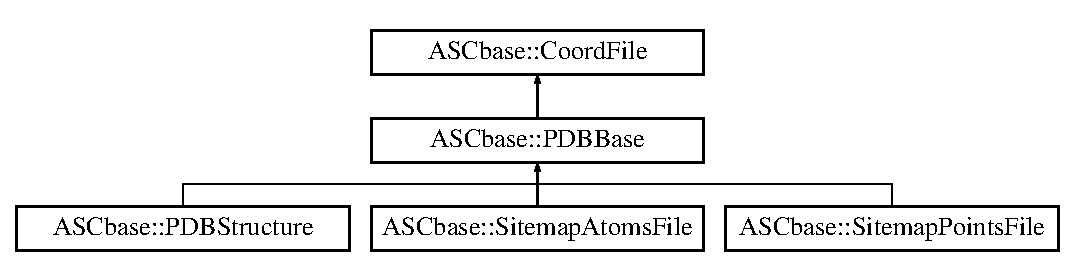
\includegraphics[height=3cm]{classASCbase_1_1PDBBase}
\end{center}
\end{figure}
\subsection*{Public Types}
\begin{CompactItemize}
\item 
typedef std::vector$<$ \bf{modres\_\-record\_\-type} $>$ \textbf{modres\_\-record\_\-vec}\label{classASCbase_1_1PDBBase_8d5d34b3f2916c01b64e7bc31036098b}

\item 
typedef modres\_\-record\_\-vec::iterator \textbf{modres\_\-record\_\-vi}\label{classASCbase_1_1PDBBase_350b2317b7319d666ec8e5f63d604f75}

\item 
typedef modres\_\-record\_\-vec::const\_\-iterator \textbf{modres\_\-record\_\-vci}\label{classASCbase_1_1PDBBase_c99c0ff276ac01a6424628da2c659872}

\item 
typedef std::vector$<$ \bf{het\_\-record\_\-type} $>$ \textbf{het\_\-record\_\-vec}\label{classASCbase_1_1PDBBase_61db0e7bba877dddbc56ffcfde427b23}

\item 
typedef het\_\-record\_\-vec::iterator \textbf{het\_\-record\_\-vi}\label{classASCbase_1_1PDBBase_04bbb2851e1d5cb94623b22c6290efe8}

\item 
typedef het\_\-record\_\-vec::const\_\-iterator \textbf{het\_\-record\_\-vci}\label{classASCbase_1_1PDBBase_da9851127724fcf51ca15403d73f3803}

\end{CompactItemize}
\subsection*{Public Member Functions}
\begin{CompactItemize}
\item 
\bf{PDBBase} ()\label{classASCbase_1_1PDBBase_b8a7226b098f891fff8a84c8efac0e94}

\begin{CompactList}\small\item\em Typically used to create a PDB file. \item\end{CompactList}\item 
\bf{PDBBase} (const std::string filename, const verbose\_\-level\_\-t verbosity=VERBOSE\_\-SILENT)
\begin{CompactList}\small\item\em Read in a PDB file. \item\end{CompactList}\item 
\bf{$\sim$PDBBase} ()\label{classASCbase_1_1PDBBase_d5a3b091d8d5a6e718a8ed91b2d3720d}

\begin{CompactList}\small\item\em Do nothing destructor. \item\end{CompactList}\item 
bool \bf{write} (const std::string filename)
\begin{CompactList}\small\item\em Write the atoms to file in PDB format. \item\end{CompactList}\item 
const bool \bf{const\_\-write} (const std::string filename) const \label{classASCbase_1_1PDBBase_3a17f60455b5bb35305dd7a4405930dd}

\begin{CompactList}\small\item\em entire existence is for debugging const pointers to pdb files \item\end{CompactList}\item 
bool \bf{write\_\-xyzr} (std::ostream \&out, bool include\_\-metals, const std::vector$<$ std::string $>$ \&waters)
\begin{CompactList}\small\item\em Write as xyzr lines (coordinates + radius). \item\end{CompactList}\item 
void \bf{set\_\-header} (const std::string h)
\begin{CompactList}\small\item\em Set the header. \item\end{CompactList}\item 
void \bf{report\_\-stats} (std::ostream \&out)\label{classASCbase_1_1PDBBase_7918cb94d1deb47d69fef5816e7a7782}

\begin{CompactList}\small\item\em does nothing \item\end{CompactList}\item 
modres\_\-record\_\-vci \textbf{modres\_\-records\_\-begin} () const \label{classASCbase_1_1PDBBase_011323485c71328e19088a1d63b7529c}

\item 
modres\_\-record\_\-vci \textbf{modres\_\-records\_\-end} () const \label{classASCbase_1_1PDBBase_9c75df999d4d3b5e2cf6ca398c9c37c0}

\item 
het\_\-record\_\-vci \textbf{het\_\-records\_\-begin} () const \label{classASCbase_1_1PDBBase_123db222cea71e537c127ead94792cd1}

\item 
het\_\-record\_\-vci \textbf{het\_\-records\_\-end} () const \label{classASCbase_1_1PDBBase_51ffbc4c560c201e959f162221bf9cd0}

\end{CompactItemize}
\subsection*{Static Public Member Functions}
\begin{CompactItemize}
\item 
static bool \bf{is\_\-hydrogen} (const std::string name)
\begin{CompactList}\small\item\em True if the pdb atom name is a hydrogen atom, else false. \item\end{CompactList}\item 
static pdb\_\-record\_\-type \bf{get\_\-record\_\-type} (const std::string line)
\end{CompactItemize}
\subsection*{Protected Member Functions}
\begin{CompactItemize}
\item 
bool \bf{read\_\-data} (std::ifstream \&fin)\label{classASCbase_1_1PDBBase_2c065e3bb88a3da81ba55ed4f02b3998}

\begin{CompactList}\small\item\em This is cheating, but .... I need a quick and dirty way to do this atm. \item\end{CompactList}\item 
bool \bf{read\_\-data} (std::ifstream \&fin, const bool ignore\_\-alt\-Locs)
\item 
void \bf{add\_\-het\_\-record} (atom\_\-vci atom)
\end{CompactItemize}
\subsection*{Private Member Functions}
\begin{CompactItemize}
\item 
bool \bf{get\_\-res\_\-info} (const std::string atom\_\-name, const std::string res\_\-name, \bf{atom\_\-t} $\ast$atom)
\item 
void \bf{read\_\-het\_\-record} (std::string \&het\_\-line)\label{classASCbase_1_1PDBBase_709ac8acd5d42fa1ffbb4b51c1251b03}

\begin{CompactList}\small\item\em Read a HET record and store it in the het record vector. \item\end{CompactList}\item 
void \bf{read\_\-modres\_\-record} (std::string \&modres\_\-line)\label{classASCbase_1_1PDBBase_b2935390dde55dd39526a43decee1eb7}

\begin{CompactList}\small\item\em Read a MODRES record and store it in the modres record vector. \item\end{CompactList}\end{CompactItemize}
\subsection*{Private Attributes}
\begin{CompactItemize}
\item 
het\_\-record\_\-vec \bf{A\_\-het\_\-records}\label{classASCbase_1_1PDBBase_611f815d363ce445712c8a0bf4facbb4}

\begin{CompactList}\small\item\em Vector of \char`\"{}HET   \char`\"{} records. \item\end{CompactList}\item 
modres\_\-record\_\-vec \bf{A\_\-modres\_\-records}\label{classASCbase_1_1PDBBase_6c966a768459840b7a19eacabd51d099}

\begin{CompactList}\small\item\em Vector of MODRES records. \item\end{CompactList}\item 
std::string \bf{A\_\-header}\label{classASCbase_1_1PDBBase_d97d60e884704fd46ee09111846b0989}

\begin{CompactList}\small\item\em String holding the header info. \item\end{CompactList}\end{CompactItemize}
\subsection*{Static Private Attributes}
\begin{CompactItemize}
\item 
static const std::string \bf{A\_\-fname} = \char`\"{}PDBBase.C\char`\"{}\label{classASCbase_1_1PDBBase_2abb2396c1c8ad545d6e463a8690043b}

\begin{CompactList}\small\item\em Name of source file. \item\end{CompactList}\end{CompactItemize}
\subsection*{Classes}
\begin{CompactItemize}
\item 
struct \bf{het\_\-record\_\-type}
\begin{CompactList}\small\item\em Holds the information in one HET record (line). \item\end{CompactList}\item 
struct \bf{modres\_\-record\_\-type}
\begin{CompactList}\small\item\em Holds the information in one MODRES record (line). \item\end{CompactList}\end{CompactItemize}


\subsection{Detailed Description}
Base class for reading and writing PDB coordinate files. 



\subsection{Constructor \& Destructor Documentation}
\index{ASCbase::PDBBase@{ASCbase::PDBBase}!PDBBase@{PDBBase}}
\index{PDBBase@{PDBBase}!ASCbase::PDBBase@{ASCbase::PDBBase}}
\subsubsection{\setlength{\rightskip}{0pt plus 5cm}PDBBase::PDBBase (const std::string {\em filename}, const verbose\_\-level\_\-t {\em verbosity} = {\tt VERBOSE\_\-SILENT})}\label{classASCbase_1_1PDBBase_d4be3eb331549cbbe0cbed8c74e89817}


Read in a PDB file. 

After a successful call to this constructor, the heavy atoms will be accessible by the Coord\-File::begin()/end() functions.

\begin{Desc}
\item[Parameters:]
\begin{description}
\item[{\em filename}]Path to the PDB file to read (heavy atoms) \item[{\em verbosity}]Whether to send some comments to stdout or not \end{description}
\end{Desc}


\subsection{Member Function Documentation}
\index{ASCbase::PDBBase@{ASCbase::PDBBase}!add_het_record@{add\_\-het\_\-record}}
\index{add_het_record@{add\_\-het\_\-record}!ASCbase::PDBBase@{ASCbase::PDBBase}}
\subsubsection{\setlength{\rightskip}{0pt plus 5cm}void PDBBase::add\_\-het\_\-record (atom\_\-vci {\em atom})\hspace{0.3cm}{\tt  [protected]}}\label{classASCbase_1_1PDBBase_e15bcd15e9d3d97f9b85f43a50557db7}


A number of pdb files do not have HET entries for 1 or more of the HET groups \index{ASCbase::PDBBase@{ASCbase::PDBBase}!get_record_type@{get\_\-record\_\-type}}
\index{get_record_type@{get\_\-record\_\-type}!ASCbase::PDBBase@{ASCbase::PDBBase}}
\subsubsection{\setlength{\rightskip}{0pt plus 5cm}pdb\_\-record\_\-type PDBBase::get\_\-record\_\-type (const std::string {\em line})\hspace{0.3cm}{\tt  [static]}}\label{classASCbase_1_1PDBBase_9ca7950fae493f47aa2fedb86a797d50}


\begin{Desc}
\item[Parameters:]
\begin{description}
\item[{\em line}]PDB line to test \end{description}
\end{Desc}
\begin{Desc}
\item[Returns:]PDB atom line type (not atom line, hetatm, atom or hydrogen) \end{Desc}
\index{ASCbase::PDBBase@{ASCbase::PDBBase}!get_res_info@{get\_\-res\_\-info}}
\index{get_res_info@{get\_\-res\_\-info}!ASCbase::PDBBase@{ASCbase::PDBBase}}
\subsubsection{\setlength{\rightskip}{0pt plus 5cm}bool PDBBase::get\_\-res\_\-info (const std::string {\em atom\_\-name}, const std::string {\em res\_\-name}, \bf{atom\_\-t} $\ast$ {\em atom})\hspace{0.3cm}{\tt  [private]}}\label{classASCbase_1_1PDBBase_2b49fed724fd6cc31ddd3eb804f7d89c}


Given an atom string an residue string, load the Van Der Waals radius, residue enum, atom enum and atom orbit into the given atom structure.

\begin{Desc}
\item[Parameters:]
\begin{description}
\item[{\em atom\_\-name}]4 char atom string \item[{\em res\_\-name}]3 char residue string \item[{\em atom}]Pointer to an atom structure return True if the given residue and atom strings are in table, else false \end{description}
\end{Desc}
\index{ASCbase::PDBBase@{ASCbase::PDBBase}!is_hydrogen@{is\_\-hydrogen}}
\index{is_hydrogen@{is\_\-hydrogen}!ASCbase::PDBBase@{ASCbase::PDBBase}}
\subsubsection{\setlength{\rightskip}{0pt plus 5cm}bool PDBBase::is\_\-hydrogen (const std::string {\em name})\hspace{0.3cm}{\tt  [static]}}\label{classASCbase_1_1PDBBase_6ac23db47cc859ba574c999d40d52039}


True if the pdb atom name is a hydrogen atom, else false. 

Caution: you can't just test column 14 or you will remove metals like Rh, Cd, Pd, Nd, Gd, Md...

\begin{Desc}
\item[Parameters:]
\begin{description}
\item[{\em name}]The 4 columns used to specify the ATOM/HETATM name \end{description}
\end{Desc}
\begin{Desc}
\item[Returns:]True if is hydrogen, else false \end{Desc}
\index{ASCbase::PDBBase@{ASCbase::PDBBase}!read_data@{read\_\-data}}
\index{read_data@{read\_\-data}!ASCbase::PDBBase@{ASCbase::PDBBase}}
\subsubsection{\setlength{\rightskip}{0pt plus 5cm}bool PDBBase::read\_\-data (std::ifstream \& {\em fin}, const bool {\em ignore\_\-alt\-Locs})\hspace{0.3cm}{\tt  [protected]}}\label{classASCbase_1_1PDBBase_b11b6aca971d2ce849b16ae28c9f366f}


\begin{Desc}
\item[Parameters:]
\begin{description}
\item[{\em fin}]Reference to an input pdb file stream \item[{\em ignore\_\-alt\-Locs}]If true, use only the first atomic position for each group of alternate locations \end{description}
\end{Desc}
\begin{Desc}
\item[Returns:]True if no error occured during reading, else false \end{Desc}
\index{ASCbase::PDBBase@{ASCbase::PDBBase}!set_header@{set\_\-header}}
\index{set_header@{set\_\-header}!ASCbase::PDBBase@{ASCbase::PDBBase}}
\subsubsection{\setlength{\rightskip}{0pt plus 5cm}void PDBBase::set\_\-header (const std::string {\em h})}\label{classASCbase_1_1PDBBase_e2de6eb8e6bd77dcca5d0b86847db355}


Set the header. 

\begin{Desc}
\item[Parameters:]
\begin{description}
\item[{\em h}]Header to write first in PDB file \end{description}
\end{Desc}
\index{ASCbase::PDBBase@{ASCbase::PDBBase}!write@{write}}
\index{write@{write}!ASCbase::PDBBase@{ASCbase::PDBBase}}
\subsubsection{\setlength{\rightskip}{0pt plus 5cm}bool PDBBase::write (const std::string {\em filename})\hspace{0.3cm}{\tt  [virtual]}}\label{classASCbase_1_1PDBBase_e8b78da086bcde015d96f7ac19387925}


Write the atoms to file in PDB format. 

\begin{Desc}
\item[Parameters:]
\begin{description}
\item[{\em filename}]Path to the file to truncate and write PDB atoms lines \end{description}
\end{Desc}
\begin{Desc}
\item[Returns:]True if file could be opened for writing, else false \end{Desc}


Implements \bf{ASCbase::Coord\-File} \doxyref{p.}{classASCbase_1_1CoordFile_dca3f5f45c21f85215dc380e2152b613}.\index{ASCbase::PDBBase@{ASCbase::PDBBase}!write_xyzr@{write\_\-xyzr}}
\index{write_xyzr@{write\_\-xyzr}!ASCbase::PDBBase@{ASCbase::PDBBase}}
\subsubsection{\setlength{\rightskip}{0pt plus 5cm}bool PDBBase::write\_\-xyzr (std::ostream \& {\em out}, bool {\em include\_\-metals}, const std::vector$<$ std::string $>$ \& {\em waters})}\label{classASCbase_1_1PDBBase_62a92225b2ba833627563c54efd11b7c}


Write as xyzr lines (coordinates + radius). 

\begin{Desc}
\item[Parameters:]
\begin{description}
\item[{\em out}]reference to a valid ostream \item[{\em include\_\-metals}]If false, ignore all metals in PDB file \item[{\em waters}]Vector of water molecules to include \end{description}
\end{Desc}
\begin{Desc}
\item[Returns:]True if file could be opened for writing, else false \end{Desc}


The documentation for this class was generated from the following files:\begin{CompactItemize}
\item 
PDBBase.H\item 
PDBBase.C\end{CompactItemize}

\section{ASCbase::PDBBase::het\_\-record\_\-type Struct Reference}
\label{structASCbase_1_1PDBBase_1_1het__record__type}\index{ASCbase::PDBBase::het_record_type@{ASCbase::PDBBase::het\_\-record\_\-type}}
Holds the information in one HET record (line).  


{\tt \#include $<$PDBBase.H$>$}

\subsection*{Public Member Functions}
\begin{CompactItemize}
\item 
bool \textbf{contains} (atom\_\-vci atom) const \label{structASCbase_1_1PDBBase_1_1het__record__type_bc330509162725271ba3ea107759b095}

\item 
bool \textbf{contains} (const \bf{atom\_\-t} \&atom) const \label{structASCbase_1_1PDBBase_1_1het__record__type_0b9716fa4db07e2c1f2fb6de9824462b}

\end{CompactItemize}
\subsection*{Public Attributes}
\begin{CompactItemize}
\item 
std::string \bf{het\-ID}\label{structASCbase_1_1PDBBase_1_1het__record__type_38f67500111621ed6aa96f49a1ccc566}

\begin{CompactList}\small\item\em 3 character het identifier \item\end{CompactList}\item 
char \bf{chain\-ID}\label{structASCbase_1_1PDBBase_1_1het__record__type_f375324a95c74d9124203d8a099db88f}

\begin{CompactList}\small\item\em Chain id. \item\end{CompactList}\item 
uint \bf{seq\-Num}\label{structASCbase_1_1PDBBase_1_1het__record__type_7e67fcacb534bfc058abb1f17f495dad}

\begin{CompactList}\small\item\em Residue number of the het group. \item\end{CompactList}\item 
char \bf{i\-Code}\label{structASCbase_1_1PDBBase_1_1het__record__type_e9c3b632888b75ee4aee65efe7b421ab}

\begin{CompactList}\small\item\em Insertion code. \item\end{CompactList}\item 
uint \bf{num\-Het\-Atoms}\label{structASCbase_1_1PDBBase_1_1het__record__type_62ab9f80b81042ccc0e0781c40d6d9be}

\begin{CompactList}\small\item\em Number of heteroatoms in the het group. \item\end{CompactList}\item 
std::string \bf{text}\label{structASCbase_1_1PDBBase_1_1het__record__type_3d9324eb71930e1e35944cd9d9c08f51}

\begin{CompactList}\small\item\em Additional text (column 31+). \item\end{CompactList}\end{CompactItemize}


\subsection{Detailed Description}
Holds the information in one HET record (line). 



The documentation for this struct was generated from the following file:\begin{CompactItemize}
\item 
PDBBase.H\end{CompactItemize}

\section{ASCbase::PDBBase::modres\_\-record\_\-type Struct Reference}
\label{structASCbase_1_1PDBBase_1_1modres__record__type}\index{ASCbase::PDBBase::modres_record_type@{ASCbase::PDBBase::modres\_\-record\_\-type}}
Holds the information in one MODRES record (line).  


{\tt \#include $<$PDBBase.H$>$}

\subsection*{Public Member Functions}
\begin{CompactItemize}
\item 
bool \textbf{contains} (atom\_\-vci atom) const \label{structASCbase_1_1PDBBase_1_1modres__record__type_8ec38a410ab4be9f8eb84a219628efb3}

\end{CompactItemize}
\subsection*{Public Attributes}
\begin{CompactItemize}
\item 
std::string \bf{id\-Code}\label{structASCbase_1_1PDBBase_1_1modres__record__type_6a68803756d56ad22aa52b64a0ff3c5c}

\begin{CompactList}\small\item\em PDB ID code -- included for historical reasions? \item\end{CompactList}\item 
std::string \bf{res\-Name}\label{structASCbase_1_1PDBBase_1_1modres__record__type_bed137d971bf629a1ae314a15abe02a0}

\begin{CompactList}\small\item\em HET ID of the modified residue. \item\end{CompactList}\item 
char \bf{chain\-ID}\label{structASCbase_1_1PDBBase_1_1modres__record__type_4646af5f898e7f605c660c6a03e99326}

\begin{CompactList}\small\item\em Chain ID of the modified residue. \item\end{CompactList}\item 
uint \bf{seq\-Num}\label{structASCbase_1_1PDBBase_1_1modres__record__type_8e7203fd189ff474fb4df62d4c7370a5}

\begin{CompactList}\small\item\em Residue number of the modified residue. \item\end{CompactList}\item 
char \bf{i\-Code}\label{structASCbase_1_1PDBBase_1_1modres__record__type_ce2a7c9abb09dbdb2e3bcef4e4d8452c}

\begin{CompactList}\small\item\em Insertion code. \item\end{CompactList}\item 
residue\_\-type \bf{std\-Res}\label{structASCbase_1_1PDBBase_1_1modres__record__type_875e1b41b9c3d177a3d41bbe4d629ea1}

\begin{CompactList}\small\item\em Residue that was modified (1 of the 20 amino acids). \item\end{CompactList}\item 
std::string \bf{comment}\label{structASCbase_1_1PDBBase_1_1modres__record__type_765eead7dea06482d5b3fe2dbcd4eed0}

\begin{CompactList}\small\item\em Any pertinant comments -- usually type of modfication. \item\end{CompactList}\end{CompactItemize}


\subsection{Detailed Description}
Holds the information in one MODRES record (line). 



The documentation for this struct was generated from the following file:\begin{CompactItemize}
\item 
PDBBase.H\end{CompactItemize}

\section{ASCbase::PDBStructure Class Reference}
\label{classASCbase_1_1PDBStructure}\index{ASCbase::PDBStructure@{ASCbase::PDBStructure}}
{\tt \#include $<$PDBStructure.H$>$}

Inheritance diagram for ASCbase::PDBStructure::\begin{figure}[H]
\begin{center}
\leavevmode
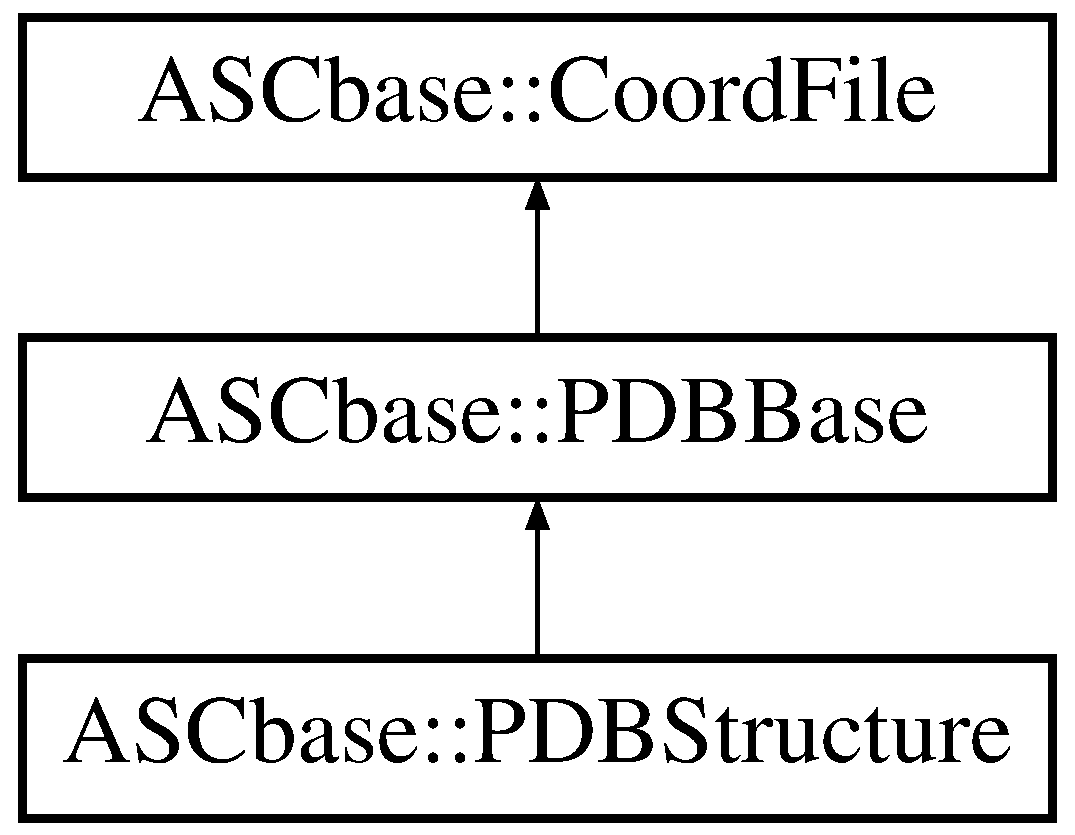
\includegraphics[height=3cm]{classASCbase_1_1PDBStructure}
\end{center}
\end{figure}
\subsection*{Public Member Functions}
\begin{CompactItemize}
\item 
\bf{PDBStructure} (const std::string filename, const bool ignore\_\-alt\-Locs=false, const verbose\_\-level\_\-t verbosity=VERBOSE\_\-SILENT)
\begin{CompactList}\small\item\em Read the heavy atoms stored in the PDB file given by filename. \item\end{CompactList}\item 
\bf{$\sim$PDBStructure} ()\label{classASCbase_1_1PDBStructure_e0882de18f1c52d18bc63f7a2853faf9}

\begin{CompactList}\small\item\em Does nothing. \item\end{CompactList}\item 
void \textbf{report\_\-stats} (std::ostream \&out, const verbose\_\-level\_\-t verbosity)\label{classASCbase_1_1PDBStructure_57ce721fcfbd2c8723e1c285cc82c3ae}

\item 
void \textbf{report\_\-hetatms} (std::ostream \&out, std::string filename)\label{classASCbase_1_1PDBStructure_37cf2f2f92078fd896a2a6eb0bccb0cc}

\item 
chain\_\-const\_\-iter \textbf{chains\_\-begin} () const \label{classASCbase_1_1PDBStructure_64aa7a5d5413c083b6ded1ba0dac64b9}

\item 
chain\_\-const\_\-iter \textbf{chains\_\-end} () const \label{classASCbase_1_1PDBStructure_84c0ba6f23d39ce0267d36c83dd90211}

\item 
residue\_\-vci \textbf{residues\_\-begin} () const \label{classASCbase_1_1PDBStructure_7caac4d414fde92934337f0b14db5b97}

\item 
residue\_\-vci \textbf{residues\_\-end} () const \label{classASCbase_1_1PDBStructure_c99ce9b93736f7144b6b1a853c79f650}

\item 
std::vector$<$ atom\_\-vci $>$::const\_\-iterator \bf{waters\_\-beg} () const \label{classASCbase_1_1PDBStructure_973302371517814e469393906b1f25bb}

\begin{CompactList}\small\item\em Get an iterator to the oxygen of the first water molecule. \item\end{CompactList}\item 
std::vector$<$ atom\_\-vci $>$::const\_\-iterator \bf{waters\_\-end} () const \label{classASCbase_1_1PDBStructure_8b5d48d05a91cd89c369a63344946844}

\begin{CompactList}\small\item\em Get an iterator to 1 past the last HOH. \item\end{CompactList}\item 
std::vector$<$ atom\_\-vci $>$::const\_\-iterator \bf{metals\_\-begin} () const \label{classASCbase_1_1PDBStructure_78b9a1980b0702359f1d574e66566f28}

\begin{CompactList}\small\item\em Get an iterator to the first metal atom. \item\end{CompactList}\item 
std::vector$<$ atom\_\-vci $>$::const\_\-iterator \bf{metals\_\-end} () const \label{classASCbase_1_1PDBStructure_0a950358cbd51702109d46334ae2a877}

\begin{CompactList}\small\item\em Get an iterator to 1 past the last metal atom. \item\end{CompactList}\item 
residue\_\-vci \textbf{get\_\-residue} (atom\_\-vci atom) const \label{classASCbase_1_1PDBStructure_f190b18c197a2d2edcd9018401ae1a0e}

\end{CompactItemize}
\subsection*{Static Public Attributes}
\begin{CompactItemize}
\item 
static const \bf{residue\_\-t} \bf{NULL\_\-RESIDUE}\label{classASCbase_1_1PDBStructure_d53c9ebfdcce8b07bab9e5fce3dd795c}

\begin{CompactList}\small\item\em the \char`\"{}standard\char`\"{} null residue \item\end{CompactList}\item 
static const residue\_\-vec \bf{NULL\_\-RESIDUE\_\-VECTOR}\label{classASCbase_1_1PDBStructure_b9016e5ccd8f6b87c0657687a77e5534}

\begin{CompactList}\small\item\em The \char`\"{}standard\char`\"{} null vector of residues -- for the null\_\-residue\_\-vci. \item\end{CompactList}\item 
static const residue\_\-vci \bf{NULL\_\-RESIDUE\_\-VCI}
\begin{CompactList}\small\item\em the \char`\"{}standard\char`\"{} null residue vector constant iterator \item\end{CompactList}\end{CompactItemize}
\subsection*{Private Member Functions}
\begin{CompactItemize}
\item 
bool \textbf{read\_\-file} (std::string filename, const bool ignore\_\-alt\-Locs)\label{classASCbase_1_1PDBStructure_b3b04d9659f89ef62e6bfccbe43ea1a6}

\item 
void \bf{form\_\-chains\_\-and\_\-residues} ()\label{classASCbase_1_1PDBStructure_51b9f8bcbf8696aa54202d67cce5d960}

\begin{CompactList}\small\item\em Create chains and residues from the atom information. \item\end{CompactList}\item 
bool \textbf{add\_\-residue} (atom\_\-vci initial\_\-atom, residue\_\-vi $\ast$current\_\-residue)\label{classASCbase_1_1PDBStructure_1e48c558b27c979aad74d972ee00ae9c}

\end{CompactItemize}
\subsection*{Private Attributes}
\begin{CompactItemize}
\item 
residue\_\-vec \bf{residues}\label{classASCbase_1_1PDBStructure_9dd11f6736cc87da3b9b89031ce80b7e}

\begin{CompactList}\small\item\em All residues in the PDB file. \item\end{CompactList}\item 
residue\_\-vec \bf{A\_\-hetgroups}\label{classASCbase_1_1PDBStructure_d42eef56f82b05db082c56d6d49ad1b6}

\begin{CompactList}\small\item\em HET entries that are not also MODRES entries. \item\end{CompactList}\item 
chain\_\-vec \bf{chains}\label{classASCbase_1_1PDBStructure_9e612a84fabe11bc13fb1765b592106d}

\begin{CompactList}\small\item\em All chains in PDB file. \item\end{CompactList}\item 
std::vector$<$ atom\_\-vci $>$ \bf{A\_\-waters}\label{classASCbase_1_1PDBStructure_7edafbe33504dcb7cc88773d9a59284c}

\begin{CompactList}\small\item\em All the waters in PDB file. \item\end{CompactList}\item 
std::vector$<$ atom\_\-vci $>$ \bf{metals}\label{classASCbase_1_1PDBStructure_04d9ef54e90699d0f17bd2b2bd06aab5}

\begin{CompactList}\small\item\em All the metals in PDB file. \item\end{CompactList}\end{CompactItemize}
\subsection*{Static Private Attributes}
\begin{CompactItemize}
\item 
static const std::string \bf{\_\-fname} = \char`\"{}PDBStructure.C\char`\"{}\label{classASCbase_1_1PDBStructure_f5b95fd62e534d4637878df12b49486e}

\begin{CompactList}\small\item\em Name of the source file. \item\end{CompactList}\end{CompactItemize}


\subsection{Detailed Description}
Basic class to impose the chain/residue/atom hierarchy of a PDB structure file. Does not contain a default constructor as we currently have no need to write structure files 



\subsection{Constructor \& Destructor Documentation}
\index{ASCbase::PDBStructure@{ASCbase::PDBStructure}!PDBStructure@{PDBStructure}}
\index{PDBStructure@{PDBStructure}!ASCbase::PDBStructure@{ASCbase::PDBStructure}}
\subsubsection{\setlength{\rightskip}{0pt plus 5cm}PDBStructure::PDBStructure (const std::string {\em filename}, const bool {\em ignore\_\-alt\-Locs} = {\tt false}, const verbose\_\-level\_\-t {\em verbosity} = {\tt VERBOSE\_\-SILENT})}\label{classASCbase_1_1PDBStructure_00a83216864911bab18d3377daf27159}


Read the heavy atoms stored in the PDB file given by filename. 

Uses \doxyref{PDBBase}{p.}{classASCbase_1_1PDBBase} to read the heavy atoms and then imposes/creates the residues and chains from the heavy atoms (in \doxyref{Coord\-File}{p.}{classASCbase_1_1CoordFile}).

\begin{Desc}
\item[Parameters:]
\begin{description}
\item[{\em filenam}]Path to the PDB structure file to read \item[{\em verbosity}]whether or not to write some stuff to stdout \end{description}
\end{Desc}


\subsection{Member Data Documentation}
\index{ASCbase::PDBStructure@{ASCbase::PDBStructure}!NULL_RESIDUE_VCI@{NULL\_\-RESIDUE\_\-VCI}}
\index{NULL_RESIDUE_VCI@{NULL\_\-RESIDUE\_\-VCI}!ASCbase::PDBStructure@{ASCbase::PDBStructure}}
\subsubsection{\setlength{\rightskip}{0pt plus 5cm}const residue\_\-vci \bf{PDBStructure::NULL\_\-RESIDUE\_\-VCI}\hspace{0.3cm}{\tt  [static]}}\label{classASCbase_1_1PDBStructure_f2758b2a1d343af8dce5d53ec61cab9a}


\textbf{Initial value:}

\begin{Code}\begin{verbatim} 
  PDBStructure::NULL_RESIDUE_VECTOR.begin()
\end{verbatim}\end{Code}
the \char`\"{}standard\char`\"{} null residue vector constant iterator 



The documentation for this class was generated from the following files:\begin{CompactItemize}
\item 
PDBStructure.H\item 
PDBStructure.C\end{CompactItemize}

\section{ASCbase::geometry::plane\_\-t Class Reference}
\label{classASCbase_1_1geometry_1_1plane__t}\index{ASCbase::geometry::plane_t@{ASCbase::geometry::plane\_\-t}}
Computational representation of an analyticaly defined 3D plane.  


{\tt \#include $<$sphere.H$>$}

\subsection*{Public Member Functions}
\begin{CompactItemize}
\item 
\bf{plane\_\-t} ()\label{classASCbase_1_1geometry_1_1plane__t_6a96b14a51383e4f04b440fa4f89ce72}

\begin{CompactList}\small\item\em Default constructor. \item\end{CompactList}\item 
\textbf{plane\_\-t} (const my\_\-float\_\-t $\ast$N, const my\_\-float\_\-t $\ast$P0)\label{classASCbase_1_1geometry_1_1plane__t_e9e131b4396c0cfd95ca45fe5e10c7fc}

\item 
\textbf{plane\_\-t} (const my\_\-float\_\-t $\ast$N, const my\_\-float\_\-t d)\label{classASCbase_1_1geometry_1_1plane__t_59a4c03593f8738e75c8058bca6ae3b5}

\item 
\textbf{plane\_\-t} (const \bf{plane\_\-t} \&src)\label{classASCbase_1_1geometry_1_1plane__t_3bcc78fa427df47158b7a929f5daf4f5}

\item 
const \bf{plane\_\-t} \& \textbf{operator=} (const \bf{plane\_\-t} \&src)\label{classASCbase_1_1geometry_1_1plane__t_52998da3f919f0dc7ad81b41ff06a6fa}

\item 
my\_\-float\_\-t \textbf{signed\_\-dist} (const my\_\-float\_\-t $\ast$pt) const \label{classASCbase_1_1geometry_1_1plane__t_d07a8d10378c09fa6e685ac904c2646d}

\item 
void \bf{intersection} (const \bf{plane\_\-t} \&other, my\_\-float\_\-t $\ast$m, my\_\-float\_\-t $\ast$b)
\begin{CompactList}\small\item\em Plane - plane intersection. \item\end{CompactList}\item 
const my\_\-float\_\-t $\ast$ \textbf{normal} () const \label{classASCbase_1_1geometry_1_1plane__t_46707f1b4f2a00ea36fc49e783d153b9}

\item 
const my\_\-float\_\-t $\ast$ \textbf{point} () const \label{classASCbase_1_1geometry_1_1plane__t_85dd05c8e741d2bb84bdf62e00831108}

\end{CompactItemize}
\subsection*{Private Member Functions}
\begin{CompactItemize}
\item 
void \textbf{do\_\-copy} (const \bf{plane\_\-t} \&src)\label{classASCbase_1_1geometry_1_1plane__t_07d9042854d890d0f1f6d67b24005944}

\end{CompactItemize}
\subsection*{Private Attributes}
\begin{CompactItemize}
\item 
my\_\-float\_\-t \bf{A\_\-N} [3]\label{classASCbase_1_1geometry_1_1plane__t_729fc8d83f6730ffccbf6ebfddaf8f77}

\begin{CompactList}\small\item\em Unit normal to the plane. \item\end{CompactList}\item 
my\_\-float\_\-t \bf{A\_\-P0} [3]\label{classASCbase_1_1geometry_1_1plane__t_9b2e543bd396510e30f8c38b95c13b43}

\begin{CompactList}\small\item\em Point on the plane -- might be full of garbage. \item\end{CompactList}\item 
my\_\-float\_\-t \bf{A\_\-d}\label{classASCbase_1_1geometry_1_1plane__t_d8acc9a64d3c29dd0f25e9a681dcb343}

\begin{CompactList}\small\item\em The d in the plane equation NX + d = 0. \item\end{CompactList}\item 
bool \textbf{A\_\-P0\_\-is\_\-defined}\label{classASCbase_1_1geometry_1_1plane__t_0d32a9703fc45b724246c824c20b8af9}

\end{CompactItemize}


\subsection{Detailed Description}
Computational representation of an analyticaly defined 3D plane. 



\subsection{Member Function Documentation}
\index{ASCbase::geometry::plane_t@{ASCbase::geometry::plane\_\-t}!intersection@{intersection}}
\index{intersection@{intersection}!ASCbase::geometry::plane_t@{ASCbase::geometry::plane\_\-t}}
\subsubsection{\setlength{\rightskip}{0pt plus 5cm}void ASCbase::geometry::plane\_\-t::intersection (const \bf{plane\_\-t} \& {\em other}, my\_\-float\_\-t $\ast$ {\em m}, my\_\-float\_\-t $\ast$ {\em b})\hspace{0.3cm}{\tt  [inline]}}\label{classASCbase_1_1geometry_1_1plane__t_aad5de4249d5e30464f69e0280f62fd3}


Plane - plane intersection. 

Numerical approximation to intersection via Mathworld plane-plane page replace this with SVD or other linear solution to [N1,N2]$^\wedge$T x = -[d1;d2] 

The documentation for this class was generated from the following file:\begin{CompactItemize}
\item 
sphere.H\end{CompactItemize}

\section{ASCbase::point\_\-and\_\-surf\_\-score Class Reference}
\label{classASCbase_1_1point__and__surf__score}\index{ASCbase::point_and_surf_score@{ASCbase::point\_\-and\_\-surf\_\-score}}
{\tt \#include $<$point\_\-and\_\-surf\_\-score.H$>$}

Inheritance diagram for ASCbase::point\_\-and\_\-surf\_\-score::\begin{figure}[H]
\begin{center}
\leavevmode
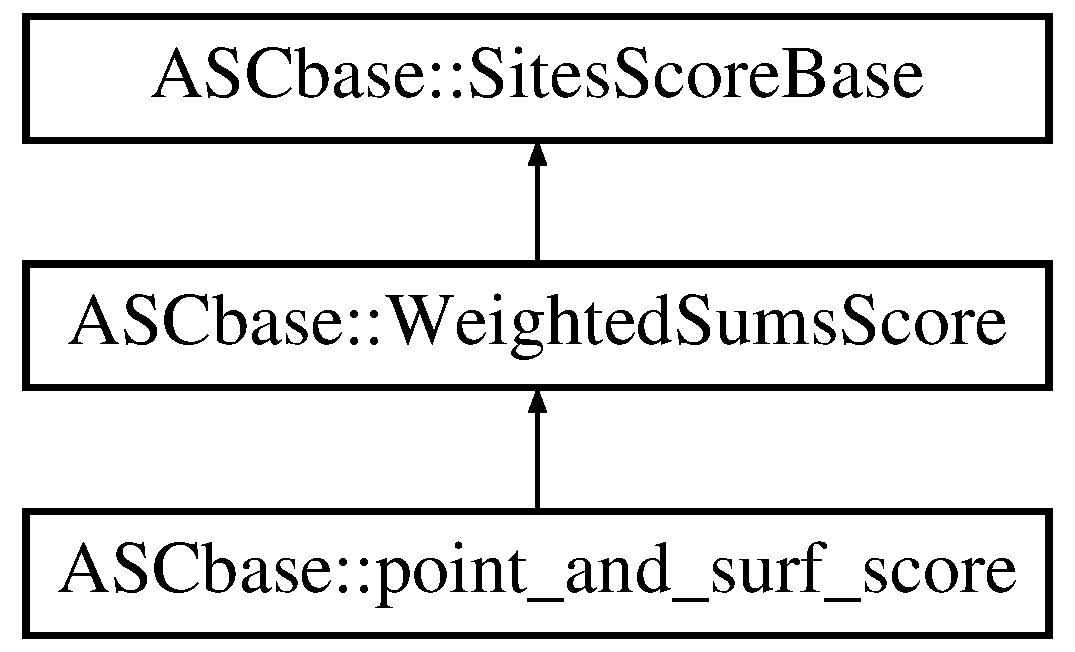
\includegraphics[height=3cm]{classASCbase_1_1point__and__surf__score}
\end{center}
\end{figure}
\subsection*{Public Types}
\begin{CompactItemize}
\item 
typedef std::less$<$ my\_\-float\_\-t $>$ \textbf{score\_\-cmp}\label{classASCbase_1_1point__and__surf__score_405dc3ab831a2a3ce477371381754ecb}

\end{CompactItemize}
\subsection*{Public Member Functions}
\begin{CompactItemize}
\item 
\bf{point\_\-and\_\-surf\_\-score} ()
\item 
virtual \bf{$\sim$point\_\-and\_\-surf\_\-score} ()\label{classASCbase_1_1point__and__surf__score_026bcdde24594caa5a97c6972054705b}

\begin{CompactList}\small\item\em basic destruction \item\end{CompactList}\item 
virtual my\_\-float\_\-t \bf{correspondences} (const \bf{Model\-Sitemap} \&model, my\_\-float\_\-t $\ast$$\ast$query\_\-pts\_\-ptr, my\_\-float\_\-t $\ast$$\ast$db\_\-pts\_\-ptr, size\_\-t $\ast$npts)\label{classASCbase_1_1point__and__surf__score_27f16e631d4e80dfc3143503a52c90ec}

\begin{CompactList}\small\item\em Get the latest correspondences of the db to query sites. \item\end{CompactList}\item 
virtual void \textbf{correspondences} (const \bf{Model\-Sitemap} \&model, std::vector$<$ const my\_\-float\_\-t $\ast$ $>$ $\ast$q\_\-pts, std::vector$<$ const my\_\-float\_\-t $\ast$ $>$ $\ast$corr\_\-pts)\label{classASCbase_1_1point__and__surf__score_80f0464267af0b9043cea9bd916c0e71}

\item 
my\_\-float\_\-t \bf{score} (const \bf{Model\-Sitemap} \&model, const \bf{Dbase\-Sitemap} \&dbase, \bf{rigid\_\-align\_\-t} $\ast$scores)
\item 
virtual bool \bf{uses\_\-surface\_\-mesh} ()
\item 
virtual bool \bf{uses\_\-hbond\_\-surfaces} ()
\end{CompactItemize}
\subsection*{Private Member Functions}
\begin{CompactItemize}
\item 
void \bf{init\_\-storage} (const geometry::Transformable\-Trimesh \&model\_\-surf)\label{classASCbase_1_1point__and__surf__score_2827297be99fcfe18648e4ea3628686c}

\begin{CompactList}\small\item\em Initialize the closest point and distance variables. \item\end{CompactList}\end{CompactItemize}
\subsection*{Private Attributes}
\begin{CompactItemize}
\item 
int \textbf{A\_\-max\_\-num\_\-verts}\label{classASCbase_1_1point__and__surf__score_c4d633ddd7fded81e725b66ba1f81686}

\item 
my\_\-float\_\-t \textbf{A\_\-max\_\-surf\_\-pt\_\-dist}\label{classASCbase_1_1point__and__surf__score_b839b589a73bd37ee51690f393e67846}

\item 
my\_\-float\_\-t $\ast$ \textbf{A\_\-surf\_\-closest\_\-pts}\label{classASCbase_1_1point__and__surf__score_c3bcfa7adb36a775e398242dbedd0657}

\item 
my\_\-float\_\-t $\ast$ \textbf{A\_\-dists}\label{classASCbase_1_1point__and__surf__score_7aa3be8f2257e8532c159a9d7eb012da}

\item 
my\_\-float\_\-t $\ast$ \textbf{A\_\-best\_\-normals}\label{classASCbase_1_1point__and__surf__score_7d7799e29bccd6da2b9b6eb023b6fe44}

\item 
my\_\-float\_\-t $\ast$ \textbf{A\_\-norm\_\-dists}\label{classASCbase_1_1point__and__surf__score_d965e1e68c8bb63bfac23e89ff10c356}

\end{CompactItemize}
\subsection*{Static Private Attributes}
\begin{CompactItemize}
\item 
static const my\_\-float\_\-t \bf{CONSTANT\_\-TERM} = -2.62899\label{classASCbase_1_1point__and__surf__score_a3a29e579d62f92126b0470c3043f3f5}

\begin{CompactList}\small\item\em Constant obtained from the regresion method. \item\end{CompactList}\item 
static const my\_\-float\_\-t \bf{POLAR\_\-SUM\_\-W} = 0.0\label{classASCbase_1_1point__and__surf__score_2216129e8311f234287371a33df97405}

\begin{CompactList}\small\item\em W for sum all \char`\"{}good\char`\"{} polar interactions. \item\end{CompactList}\item 
static const my\_\-float\_\-t \bf{POLAR\_\-MISMATCH\_\-W} = 0.0\label{classASCbase_1_1point__and__surf__score_1af29447d3e299fd97abe3d097b939d6}

\begin{CompactList}\small\item\em W for sum of AD or DA matches with positive dot product. \item\end{CompactList}\item 
static const my\_\-float\_\-t \bf{DD\_\-OR\_\-AA\_\-POLAR\_\-SUM\_\-W} = -0.0122689\label{classASCbase_1_1point__and__surf__score_9a704a57b1f9eb9e9f6ac068c853ce39}

\begin{CompactList}\small\item\em W for sum only DD or AA \char`\"{}good\char`\"{} polar interactions. \item\end{CompactList}\item 
static const my\_\-float\_\-t \bf{DONEPTOR\_\-POLAR\_\-SUM\_\-W} = -0.00619202\label{classASCbase_1_1point__and__surf__score_56855cb7161ed00c8659efd884748277}

\begin{CompactList}\small\item\em W for sum NA or AN or ND or DN or NN \char`\"{}good\char`\"{} polar interactions. \item\end{CompactList}\item 
static const my\_\-float\_\-t \bf{HPHOBIC\_\-COUNT\_\-W} = 0.0\label{classASCbase_1_1point__and__surf__score_8f072355012a706395ffe3e0a169866b}

\begin{CompactList}\small\item\em W for hydrophobic point count. \item\end{CompactList}\item 
static const my\_\-float\_\-t \bf{UNSAT\_\-POLAR\_\-W} = 0.0\label{classASCbase_1_1point__and__surf__score_97c1da0c6d8565d1c332d686bc789b75}

\begin{CompactList}\small\item\em W for polar points matched to hydrophobic. \item\end{CompactList}\item 
static const my\_\-float\_\-t \textbf{SURFACE\_\-RMSE\_\-W} = 2.11849\label{classASCbase_1_1point__and__surf__score_eabec3fdd01002f2115afdc5b34bbf61}

\item 
static const my\_\-float\_\-t \bf{SCALED\_\-CONSTANT\_\-TERM} = -2.70337\label{classASCbase_1_1point__and__surf__score_8b4842d2249c43f9a34209a3617459eb}

\begin{CompactList}\small\item\em Constant obtained from the regresion method for scaled terms. \item\end{CompactList}\item 
static const my\_\-float\_\-t \bf{SCALED\_\-POLAR\_\-SUM\_\-W} = 0.0\label{classASCbase_1_1point__and__surf__score_216b3496bf9f25b543a7cab6847fe903}

\begin{CompactList}\small\item\em W for sum all \char`\"{}good\char`\"{} polar interactions for scaled terms. \item\end{CompactList}\item 
static const my\_\-float\_\-t \bf{SCALED\_\-POLAR\_\-MISMATCH\_\-W} = 0.0\label{classASCbase_1_1point__and__surf__score_8bf9f0a1f299ada21900bd2d768efd86}

\begin{CompactList}\small\item\em W for sum of AD or DA matches with positive dot product for scaled terms. \item\end{CompactList}\item 
static const my\_\-float\_\-t \bf{SCALED\_\-DD\_\-OR\_\-AA\_\-POLAR\_\-SUM\_\-W} = -0.237545\label{classASCbase_1_1point__and__surf__score_69e09360f0b135074a1e1bb9ea7bea43}

\begin{CompactList}\small\item\em W for sum only DD or AA \char`\"{}good\char`\"{} polar interactions for scaled terms. \item\end{CompactList}\item 
static const my\_\-float\_\-t \bf{SCALED\_\-DONEPTOR\_\-POLAR\_\-SUM\_\-W} = 0.0471545\label{classASCbase_1_1point__and__surf__score_c021b19d8d595f7f8cf163893e4f0aab}

\begin{CompactList}\small\item\em W for sum NA or AN or ND or DN or NN \char`\"{}good\char`\"{} polar interactions for scaled terms. \item\end{CompactList}\item 
static const my\_\-float\_\-t \bf{SCALED\_\-HPHOBIC\_\-COUNT\_\-W} = 0.0\label{classASCbase_1_1point__and__surf__score_b1ec6fe89fa9ae82f06e05bf80c7cd80}

\begin{CompactList}\small\item\em W for hydrophobic point count for scaled terms. \item\end{CompactList}\item 
static const my\_\-float\_\-t \bf{SCALED\_\-UNSAT\_\-POLAR\_\-W} = 0.0\label{classASCbase_1_1point__and__surf__score_573a682441a39d1ca6ebb6542e2154b6}

\begin{CompactList}\small\item\em W for polar points matched to hydrophobic for scaled terms. \item\end{CompactList}\item 
static const my\_\-float\_\-t \textbf{SCALED\_\-SURFACE\_\-RMSE\_\-W} = 3.25161\label{classASCbase_1_1point__and__surf__score_30dc1ab5839522ac2c04b516a4cb7392}

\item 
static const int \textbf{A\_\-num\_\-terms} = 6\label{classASCbase_1_1point__and__surf__score_19e2dc6aa61fb35905f6c10b36cec903}

\item 
static const std::string \bf{A\_\-fname} = \char`\"{}point\_\-and\_\-surf\_\-score.C\char`\"{}\label{classASCbase_1_1point__and__surf__score_e571b139cb9e224cba021b221d815dc1}

\begin{CompactList}\small\item\em Source file name. \item\end{CompactList}\end{CompactItemize}


\subsection{Detailed Description}
Test class for scoring rigid alignments of dbase sitemaps to a given model using both point and surface features 



\subsection{Constructor \& Destructor Documentation}
\index{ASCbase::point_and_surf_score@{ASCbase::point\_\-and\_\-surf\_\-score}!point_and_surf_score@{point\_\-and\_\-surf\_\-score}}
\index{point_and_surf_score@{point\_\-and\_\-surf\_\-score}!ASCbase::point_and_surf_score@{ASCbase::point\_\-and\_\-surf\_\-score}}
\subsubsection{\setlength{\rightskip}{0pt plus 5cm}point\_\-and\_\-surf\_\-score::point\_\-and\_\-surf\_\-score ()}\label{classASCbase_1_1point__and__surf__score_81703ab3d5c6d6181e528d2a751725b5}


Default constructor for site map point scoring and surface mesh scoring of (aligned) site maps 

\subsection{Member Function Documentation}
\index{ASCbase::point_and_surf_score@{ASCbase::point\_\-and\_\-surf\_\-score}!score@{score}}
\index{score@{score}!ASCbase::point_and_surf_score@{ASCbase::point\_\-and\_\-surf\_\-score}}
\subsubsection{\setlength{\rightskip}{0pt plus 5cm}my\_\-float\_\-t ASCbase::point\_\-and\_\-surf\_\-score::score (const \bf{Model\-Sitemap} \& {\em model}, const \bf{Dbase\-Sitemap} \& {\em dbase}, \bf{rigid\_\-align\_\-t} $\ast$ {\em scores})\hspace{0.3cm}{\tt  [inline, virtual]}}\label{classASCbase_1_1point__and__surf__score_f7086e180c849bba8a8a1df984a3b114}


\begin{Desc}
\item[Parameters:]
\begin{description}
\item[{\em model}]Const ref to the model site \item[{\em dbase}]Const ref to the sitemap aligned to the model sitemap \item[{\em scores}]iterator to the score data class \end{description}
\end{Desc}
\begin{Desc}
\item[Returns:]The score of the alignment \end{Desc}


Reimplemented from \bf{ASCbase::Weighted\-Sums\-Score} \doxyref{p.}{classASCbase_1_1WeightedSumsScore_eeee8c834449ce75686bb076f40c3ee4}.\index{ASCbase::point_and_surf_score@{ASCbase::point\_\-and\_\-surf\_\-score}!uses_hbond_surfaces@{uses\_\-hbond\_\-surfaces}}
\index{uses_hbond_surfaces@{uses\_\-hbond\_\-surfaces}!ASCbase::point_and_surf_score@{ASCbase::point\_\-and\_\-surf\_\-score}}
\subsubsection{\setlength{\rightskip}{0pt plus 5cm}virtual bool ASCbase::point\_\-and\_\-surf\_\-score::uses\_\-hbond\_\-surfaces ()\hspace{0.3cm}{\tt  [inline, virtual]}}\label{classASCbase_1_1point__and__surf__score_8f006a0249c062673acec07465b4d686}


Derived class should return false, unless the derived class is using the hydrogen bond surface caps 

Reimplemented from \bf{ASCbase::Weighted\-Sums\-Score} \doxyref{p.}{classASCbase_1_1WeightedSumsScore_a54a5a22b71dd4bc14aaf06f7756eca7}.\index{ASCbase::point_and_surf_score@{ASCbase::point\_\-and\_\-surf\_\-score}!uses_surface_mesh@{uses\_\-surface\_\-mesh}}
\index{uses_surface_mesh@{uses\_\-surface\_\-mesh}!ASCbase::point_and_surf_score@{ASCbase::point\_\-and\_\-surf\_\-score}}
\subsubsection{\setlength{\rightskip}{0pt plus 5cm}virtual bool ASCbase::point\_\-and\_\-surf\_\-score::uses\_\-surface\_\-mesh ()\hspace{0.3cm}{\tt  [inline, virtual]}}\label{classASCbase_1_1point__and__surf__score_92345073d3e38666cb95cca9adc14ae3}


Derived class should return false, unless, the site's surface needs to be to be rotated and translated 

Reimplemented from \bf{ASCbase::Weighted\-Sums\-Score} \doxyref{p.}{classASCbase_1_1WeightedSumsScore_9d12b648a5adc7dff9d6058d6239a314}.

The documentation for this class was generated from the following files:\begin{CompactItemize}
\item 
point\_\-and\_\-surf\_\-score.H\item 
point\_\-and\_\-surf\_\-score.C\end{CompactItemize}

\section{ASCbase::point\_\-bins$<$ \_\-Tp $>$ Class Template Reference}
\label{classASCbase_1_1point__bins}\index{ASCbase::point_bins@{ASCbase::point\_\-bins}}
Divide up the space based on a coordinate aligned grid.  


{\tt \#include $<$point\_\-bins.H$>$}

\subsection*{Public Types}
\begin{CompactItemize}
\item 
typedef std::vector$<$ point\_\-bin\_\-t$<$ \_\-Tp $>$ $>$ \textbf{bin\_\-vec}\label{classASCbase_1_1point__bins_dfb6ebb20eb7f4497553a21504367efa}

\item 
typedef bin\_\-vec::iterator \textbf{bin\_\-vi}\label{classASCbase_1_1point__bins_2612ddc643a2f477309393a2c8ded71c}

\item 
typedef bin\_\-vec::const\_\-iterator \textbf{bin\_\-vci}\label{classASCbase_1_1point__bins_32892df5e6abb8c0d4241ef6ed439604}

\item 
typedef std::multimap$<$ bin\_\-vci, const my\_\-float\_\-t $\ast$ $>$ \textbf{bin2vert\_\-mmap}\label{classASCbase_1_1point__bins_39a6b59e9bbd2dea53aa1715e9729edf}

\end{CompactItemize}
\subsection*{Public Member Functions}
\begin{CompactItemize}
\item 
\bf{point\_\-bins} ()
\item 
\textbf{point\_\-bins} (\_\-Tp begin, \_\-Tp end, my\_\-float\_\-t bin\_\-width=4.5)\label{classASCbase_1_1point__bins_612dc97af37ea4512699f0fc0d47c61a}

\item 
\textbf{point\_\-bins} (const \bf{point\_\-bins}$<$ \_\-Tp $>$ \&other)\label{classASCbase_1_1point__bins_d2ed01481c90b33ff07f0668e039e89f}

\item 
const \bf{point\_\-bins} \& \textbf{operator=} (const \bf{point\_\-bins} \&other)\label{classASCbase_1_1point__bins_ec766713f1c00b6cca41d52940f91050}

\item 
void \textbf{setup\_\-grid} (\_\-Tp begin, \_\-Tp end, const my\_\-float\_\-t bin\_\-width)\label{classASCbase_1_1point__bins_8a32f681bd20aa78a9b1cd3c0773be1e}

\item 
void \bf{transform\_\-bins} (const my\_\-float\_\-t $\ast$R, const my\_\-float\_\-t $\ast$T)
\begin{CompactList}\small\item\em Transform the bins. \item\end{CompactList}\item 
void \textbf{inverse\_\-transform\_\-bins} (const my\_\-float\_\-t $\ast$R, const my\_\-float\_\-t $\ast$T)\label{classASCbase_1_1point__bins_ecf57c0678d1fec450842dfef3b81a97}

\item 
void \textbf{revert} ()\label{classASCbase_1_1point__bins_a68b236a6dcfb2a1d344ae6b2cf3a7e3}

\item 
void \textbf{get\_\-min\_\-max\_\-coords} (\_\-Tp begin, \_\-Tp end, my\_\-float\_\-t $\ast$min\_\-pos, my\_\-float\_\-t $\ast$max\_\-pos)\label{classASCbase_1_1point__bins_00ff5e0a19964585b8e01189e0ca0f82}

\item 
void \bf{determine\_\-space} (const my\_\-float\_\-t $\ast$min\_\-pos, const my\_\-float\_\-t $\ast$max\_\-pos, my\_\-float\_\-t $\ast$min\_\-corner, my\_\-float\_\-t $\ast$max\_\-corner, int $\ast$num\_\-bins)
\item 
void \textbf{populate\_\-grid} (\_\-Tp begin, \_\-Tp end, const my\_\-float\_\-t bin\_\-width, bin\_\-vec $\ast$bins)\label{classASCbase_1_1point__bins_6535d13b3b00438158656471f67a44c6}

\item 
void \textbf{get\_\-bin} (const my\_\-float\_\-t $\ast$pt, bin\_\-vci $\ast$nbrs, bin\_\-vci $\ast$moved\_\-nbrs) const \label{classASCbase_1_1point__bins_3efe4ebd6c36993e1be9802c8edf1c35}

\item 
bin\_\-vci \bf{bins\_\-end} () const \label{classASCbase_1_1point__bins_f9c9f7b5c7be74b76b0eba306879324d}

\begin{CompactList}\small\item\em Constant iterator to one past the last bin in the vector. \item\end{CompactList}\item 
bin\_\-vci \bf{moved\_\-bins\_\-end} () const \label{classASCbase_1_1point__bins_54a580e492ce7205e0bc5fc58f4bf26a}

\begin{CompactList}\small\item\em Constant iterator to one past the last bin in the vector. \item\end{CompactList}\item 
const bool \textbf{bins\_\-are\_\-setup} () const \label{classASCbase_1_1point__bins_c748633d67a3d339c7a895b43666aec1}

\item 
void \bf{update\_\-point\_\-bin} (\_\-Tp \&data)\label{classASCbase_1_1point__bins_e07134e8f4497da13dd6136bcb45602e}

\begin{CompactList}\small\item\em Check if the given data point needs to have its bins updated. \item\end{CompactList}\item 
void \textbf{remove\_\-moved\_\-points\_\-from\_\-bins} ()\label{classASCbase_1_1point__bins_5729496a671be351b0826b5452770e06}

\item 
void \textbf{write\_\-bounds} (std::ostream \&out) const \label{classASCbase_1_1point__bins_701b0831628d6b9e7e2b878da1488bd6}

\end{CompactItemize}
\subsection*{Private Member Functions}
\begin{CompactItemize}
\item 
\textbf{\_\-\_\-glibcpp\_\-class\_\-requires} (\_\-Tp, \_\-Forward\-Iterator\-Concept)\label{classASCbase_1_1point__bins_59eab23f4ede0549e5ca1a44b58f9588}

\item 
void \textbf{init} ()\label{classASCbase_1_1point__bins_2de8967933c976d7e8569695ced43111}

\item 
void \bf{do\_\-copy} (const \bf{point\_\-bins}$<$ \_\-Tp $>$ \&src)
\begin{CompactList}\small\item\em Copies could be expensive, but depend greatly on the template parameter. \item\end{CompactList}\item 
bool \textbf{get\_\-bin\_\-idz} (const my\_\-float\_\-t $\ast$pt, int $\ast$idx) const \label{classASCbase_1_1point__bins_1a6812d16a3aed4df67ea89b4ef3795b}

\end{CompactItemize}
\subsection*{Private Attributes}
\begin{CompactItemize}
\item 
\_\-Tp \textbf{A\_\-begin}\label{classASCbase_1_1point__bins_143c4437ed0bc651257efcfad94675da}

\item 
\_\-Tp \textbf{A\_\-end}\label{classASCbase_1_1point__bins_47b57104346abc683d5ab5158c42369d}

\item 
bool \textbf{A\_\-bins\_\-are\_\-setup}\label{classASCbase_1_1point__bins_7d80fecfcd4518db8d4a32cd093dfd4c}

\item 
my\_\-float\_\-t \bf{A\_\-bin\_\-width}\label{classASCbase_1_1point__bins_6ffd0913f0c0588e3c2ce19d1f4a96e3}

\begin{CompactList}\small\item\em Side length of a bin. \item\end{CompactList}\item 
my\_\-float\_\-t \bf{A\_\-bin\_\-width\_\-inv}\label{classASCbase_1_1point__bins_4fde2008e3f81fb68191c68127c20443}

\begin{CompactList}\small\item\em multiplicative inverse (1 over) side length \item\end{CompactList}\item 
my\_\-float\_\-t \textbf{A\_\-upper\_\-corner} [3]\label{classASCbase_1_1point__bins_313de0207d76bd11771307cf40f14729}

\item 
my\_\-float\_\-t \textbf{A\_\-lower\_\-corner} [3]\label{classASCbase_1_1point__bins_9ee31e608013306e3dd0416bd3813e84}

\item 
my\_\-float\_\-t \bf{A\_\-orig\_\-lower} [3]\label{classASCbase_1_1point__bins_274999e259918f2b0b5d3c2ba58435cb}

\begin{CompactList}\small\item\em Save the original lower corner. \item\end{CompactList}\item 
my\_\-float\_\-t \bf{A\_\-orig\_\-upper} [3]\label{classASCbase_1_1point__bins_6a3cf278675b515ed22a9bdfdf216784}

\begin{CompactList}\small\item\em Save the original upper corner. \item\end{CompactList}\item 
my\_\-float\_\-t \textbf{A\_\-plane\_\-normals} [9]\label{classASCbase_1_1point__bins_cebae3f68f32e3ad48fb3671718af31c}

\item 
bool \textbf{A\_\-bins\_\-are\_\-transformed}\label{classASCbase_1_1point__bins_86ca99c80831c972f89b0b20a185c519}

\item 
int \textbf{A\_\-num\_\-bins} [3]\label{classASCbase_1_1point__bins_0e3467b19cfeec3ac7590c10359489b9}

\item 
bin\_\-vec \textbf{A\_\-bins}\label{classASCbase_1_1point__bins_2297473c684667dd9f33619dabb50095}

\item 
bin\_\-vec \textbf{A\_\-bins\_\-of\_\-moved\_\-pts}\label{classASCbase_1_1point__bins_4fc0db7bdcd0d6ca24626a770899ec73}

\item 
std::vector$<$ three\_\-idz $>$ \textbf{A\_\-current\_\-bin\_\-idz}\label{classASCbase_1_1point__bins_2026dd01beaac118d479d1649ca4c1f4}

\item 
std::vector$<$ three\_\-idz $>$ \textbf{A\_\-orig\_\-bin\_\-idz}\label{classASCbase_1_1point__bins_01f7a076413e0ade2db4a8b808e18416}

\end{CompactItemize}
\subsection*{Classes}
\begin{CompactItemize}
\item 
struct \textbf{point\_\-bin\_\-t}
\item 
struct \textbf{three\_\-idz}
\end{CompactItemize}


\subsection{Detailed Description}
\subsubsection*{template$<$typename \_\-Tp$>$ class ASCbase::point\_\-bins$<$ \_\-Tp $>$}

Divide up the space based on a coordinate aligned grid. 

Assumptions: The positions may be transformed via a rigid transformation. The type \_\-Tp has a field \char`\"{}pos\char`\"{} that holds the 3D position of the type. It is expected that this will be used for the query sites; for that reason it is not necessarily optimized for speed of construction. 



\subsection{Constructor \& Destructor Documentation}
\index{ASCbase::point_bins@{ASCbase::point\_\-bins}!point_bins@{point\_\-bins}}
\index{point_bins@{point\_\-bins}!ASCbase::point_bins@{ASCbase::point\_\-bins}}
\subsubsection{\setlength{\rightskip}{0pt plus 5cm}template$<$typename \_\-Tp$>$ \bf{ASCbase::point\_\-bins}$<$ \_\-Tp $>$::\bf{point\_\-bins} ()\hspace{0.3cm}{\tt  [inline]}}\label{classASCbase_1_1point__bins_3e8b2c7e86f5ee787cc71f32cc8619da}


Default constructor -- sometimes the array cannot be constructed at class construction 

\subsection{Member Function Documentation}
\index{ASCbase::point_bins@{ASCbase::point\_\-bins}!determine_space@{determine\_\-space}}
\index{determine_space@{determine\_\-space}!ASCbase::point_bins@{ASCbase::point\_\-bins}}
\subsubsection{\setlength{\rightskip}{0pt plus 5cm}template$<$typename \_\-Tp$>$ void \bf{ASCbase::point\_\-bins}$<$ \_\-Tp $>$::determine\_\-space (const my\_\-float\_\-t $\ast$ {\em min\_\-pos}, const my\_\-float\_\-t $\ast$ {\em max\_\-pos}, my\_\-float\_\-t $\ast$ {\em min\_\-corner}, my\_\-float\_\-t $\ast$ {\em max\_\-corner}, int $\ast$ {\em num\_\-bins})\hspace{0.3cm}{\tt  [inline]}}\label{classASCbase_1_1point__bins_d0e79de47eb796a1d310e8ecf3edf3b5}


\index{ASCbase::point_bins@{ASCbase::point\_\-bins}!do_copy@{do\_\-copy}}
\index{do_copy@{do\_\-copy}!ASCbase::point_bins@{ASCbase::point\_\-bins}}
\subsubsection{\setlength{\rightskip}{0pt plus 5cm}template$<$typename \_\-Tp$>$ void \bf{ASCbase::point\_\-bins}$<$ \_\-Tp $>$::do\_\-copy (const \bf{point\_\-bins}$<$ \_\-Tp $>$ \& {\em src})\hspace{0.3cm}{\tt  [inline, private]}}\label{classASCbase_1_1point__bins_94b59a7f0902763acb6004b2f208418e}


Copies could be expensive, but depend greatly on the template parameter. 

We are assuming that most uses will have template parameters that are pointers or iterators (hence we assume \_\-Tp-$>$pos exists and is a valid 3D point). \index{ASCbase::point_bins@{ASCbase::point\_\-bins}!transform_bins@{transform\_\-bins}}
\index{transform_bins@{transform\_\-bins}!ASCbase::point_bins@{ASCbase::point\_\-bins}}
\subsubsection{\setlength{\rightskip}{0pt plus 5cm}template$<$typename \_\-Tp$>$ void \bf{ASCbase::point\_\-bins}$<$ \_\-Tp $>$::transform\_\-bins (const my\_\-float\_\-t $\ast$ {\em R}, const my\_\-float\_\-t $\ast$ {\em T})\hspace{0.3cm}{\tt  [inline]}}\label{classASCbase_1_1point__bins_ae0c63c318c55d37a6abf7f8760f0bd9}


Transform the bins. 

NOTE: this does not transform the positions, and must be used in conjunction with moving of the positions 

The documentation for this class was generated from the following file:\begin{CompactItemize}
\item 
point\_\-bins.H\end{CompactItemize}

\section{ASCbase::point\_\-storage$<$ \_\-Tp, \_\-Sequence $>$ Class Template Reference}
\label{classASCbase_1_1point__storage}\index{ASCbase::point_storage@{ASCbase::point\_\-storage}}
{\tt \#include $<$point\_\-storage.H$>$}

Inheritance diagram for ASCbase::point\_\-storage$<$ \_\-Tp, \_\-Sequence $>$::\begin{figure}[H]
\begin{center}
\leavevmode
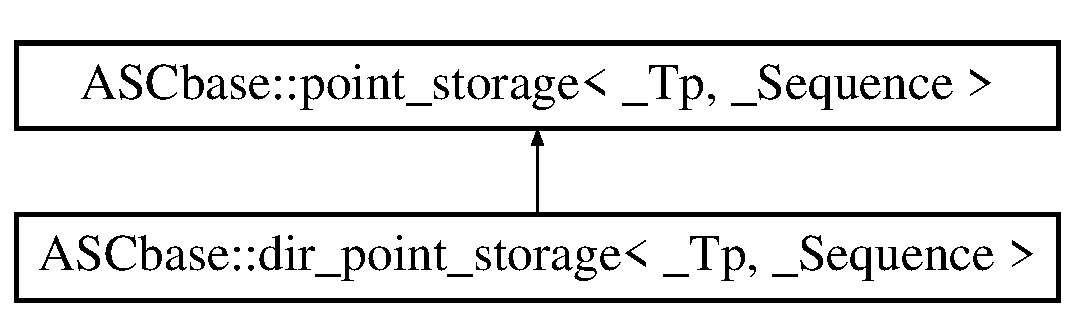
\includegraphics[height=2cm]{classASCbase_1_1point__storage}
\end{center}
\end{figure}
\subsection*{Public Types}
\begin{CompactItemize}
\item 
typedef \_\-Sequence::value\_\-type \textbf{value\_\-type}\label{classASCbase_1_1point__storage_52ae4f4fb47a9352aeb60e416b941370}

\item 
typedef \_\-Sequence::reference \textbf{reference}\label{classASCbase_1_1point__storage_2dd7aae8e2a9df9b81d20345dbf07c91}

\item 
typedef \_\-Sequence::const\_\-reference \textbf{const\_\-reference}\label{classASCbase_1_1point__storage_3929df48b7e2b43058fd8043253d1ce7}

\item 
typedef \_\-Sequence::iterator \textbf{iterator}\label{classASCbase_1_1point__storage_8ee8417d3261ab75b8de308ee0d63887}

\item 
typedef \_\-Sequence::const\_\-iterator \textbf{const\_\-iterator}\label{classASCbase_1_1point__storage_7f6d8335405d11572ea1bf048d3dabc9}

\item 
typedef \_\-Sequence::size\_\-type \textbf{size\_\-type}\label{classASCbase_1_1point__storage_7c34ddf2fad492932e2cdf5c8df2d329}

\item 
typedef \_\-Sequence::iterator::iterator\_\-category \textbf{iterator\_\-category}\label{classASCbase_1_1point__storage_462445b8c65a8df8a42b78041689caba}

\item 
typedef \_\-Sequence \textbf{container\_\-type}\label{classASCbase_1_1point__storage_3b7cb477bcd92d1bb9915a2a7b9b00ee}

\item 
typedef \bf{point\_\-bins}$<$ const\_\-iterator $>$::bin\_\-vci \textbf{bins\_\-vci\_\-type}\label{classASCbase_1_1point__storage_35749c1a56a9353992d0b6a29b67b33c}

\item 
typedef \bf{point\_\-bins}$<$ const\_\-iterator $>$ \textbf{bins\_\-type}\label{classASCbase_1_1point__storage_75ce41cf8c33f143c1c30075c5991405}

\item 
typedef std::pair$<$ my\_\-float\_\-t, const\_\-iterator $>$ \textbf{float\_\-const\_\-iter\_\-pair}\label{classASCbase_1_1point__storage_e23bb4488db360e26280b065dcb7b225}

\item 
typedef std::multimap$<$ my\_\-float\_\-t, const\_\-iterator $>$ \textbf{float\_\-const\_\-iter\_\-map}\label{classASCbase_1_1point__storage_e20eff69bd4e8a3bc7739e7339fab66d}

\end{CompactItemize}
\subsection*{Public Member Functions}
\begin{CompactItemize}
\item 
\textbf{point\_\-storage} (uint init\_\-num\_\-pts=150, uint stride\_\-in=3)\label{classASCbase_1_1point__storage_487c979dfa93bedf323e6e3a26a7786a}

\item 
\textbf{point\_\-storage} (const \bf{point\_\-storage} \&src)\label{classASCbase_1_1point__storage_dd6e131042145021e1cd7202bcfccea7}

\item 
const \bf{point\_\-storage} \& \textbf{operator=} (const \bf{point\_\-storage} \&src)\label{classASCbase_1_1point__storage_3520cbd7a09d6803b971ddb611228726}

\item 
const my\_\-float\_\-t $\ast$ \bf{points\_\-begin} () const \label{classASCbase_1_1point__storage_4179b369dfa5b1277da5db9e3e9cb0c1}

\begin{CompactList}\small\item\em Constant pointer to the beginning of the points array. \item\end{CompactList}\item 
const my\_\-float\_\-t $\ast$ \bf{points\_\-end} () const \label{classASCbase_1_1point__storage_5406affe211bf9c423b577b6bb282b56}

\begin{CompactList}\small\item\em Constant pointer to one past the end of the points array. \item\end{CompactList}\item 
const\_\-iterator \bf{begin} () const \label{classASCbase_1_1point__storage_137cc46a9b6a9eed4a2966b1c2652802}

\begin{CompactList}\small\item\em Constant iterator to the beginning of the container. \item\end{CompactList}\item 
const\_\-iterator \bf{end} () const \label{classASCbase_1_1point__storage_55e058eb0fc22f701fd441641cd49d83}

\begin{CompactList}\small\item\em Constant iterator to 1 past the end of the container. \item\end{CompactList}\item 
iterator \bf{begin} ()\label{classASCbase_1_1point__storage_83805a7e465cb05a7d94f42bd14d3626}

\begin{CompactList}\small\item\em Iterator to the beginning of the container. \item\end{CompactList}\item 
iterator \bf{end} ()\label{classASCbase_1_1point__storage_9385b69e57a30908b798d1b7aea79437}

\begin{CompactList}\small\item\em Iterator to 1 past the end of the container. \item\end{CompactList}\item 
size\_\-type \bf{size} () const \label{classASCbase_1_1point__storage_598615e1ca68e12e1f7ae8446758e608}

\begin{CompactList}\small\item\em Get the size of the container. \item\end{CompactList}\item 
void \bf{push\_\-back} (const value\_\-type \&\_\-\_\-x)
\item 
iterator \bf{erase} (iterator \_\-\_\-i)\label{classASCbase_1_1point__storage_257e54a362a5f8eab82b0d431f671903}

\begin{CompactList}\small\item\em Erase the element pointed to by the iterator. \item\end{CompactList}\item 
void \bf{transform} (const my\_\-float\_\-t $\ast$R, const my\_\-float\_\-t $\ast$T)\label{classASCbase_1_1point__storage_f90d2e349c29b237403efe80c4377a2a}

\begin{CompactList}\small\item\em Apply a rigid body transformation to the points (current positions). \item\end{CompactList}\item 
void \bf{inverse\_\-transform} (const my\_\-float\_\-t $\ast$R, const my\_\-float\_\-t $\ast$T)\label{classASCbase_1_1point__storage_20a59aecf6978920fa2bcf8be845dfc0}

\begin{CompactList}\small\item\em Apply a rigid body transformation to the points (current positions). \item\end{CompactList}\item 
void \bf{revert} ()\label{classASCbase_1_1point__storage_f08419a1ed01d6bc8de1486a5811da83}

\begin{CompactList}\small\item\em Revert the positions to the original positions. \item\end{CompactList}\item 
void \bf{set\_\-current\_\-positions\_\-as\_\-original} ()
\item 
void \bf{get\_\-current\_\-inverse\_\-3D\_\-transform} (Quaternion $\ast$Q, my\_\-float\_\-t $\ast$T) const \label{classASCbase_1_1point__storage_a8b7d0c0bc834f02e4ad877b8dc1f147}

\begin{CompactList}\small\item\em Get transform to move current positions to their original positions. \item\end{CompactList}\item 
my\_\-float\_\-t \bf{compute\_\-RMSD} () const 
\item 
const bool \bf{centroid\_\-3D} (my\_\-float\_\-t $\ast$C) const \label{classASCbase_1_1point__storage_66a712bb966c3433d12563eca592be2a}

\begin{CompactList}\small\item\em Compute the centroid of the positions. \item\end{CompactList}\item 
const\_\-iterator \bf{closest\_\-point} (const my\_\-float\_\-t $\ast$a\_\-pos, my\_\-float\_\-t $\ast$d\_\-out) const 
\item 
const\_\-iterator \bf{\_\-closest\_\-point} (const my\_\-float\_\-t $\ast$a\_\-pos, my\_\-float\_\-t $\ast$d\_\-out, std::random\_\-access\_\-iterator\_\-tag tag) const \label{classASCbase_1_1point__storage_3bc1d840ac575c316bfea6fb23d75507}

\begin{CompactList}\small\item\em Random access iterator version of closest\_\-point. \item\end{CompactList}\item 
const\_\-iterator \bf{\_\-closest\_\-point} (const my\_\-float\_\-t $\ast$a\_\-pos, my\_\-float\_\-t $\ast$d\_\-out, std::forward\_\-iterator\_\-tag tag) const \label{classASCbase_1_1point__storage_96b7602e9af5661fdd0ba9f674c55f00}

\begin{CompactList}\small\item\em Forward iterator version of closest\_\-point. \item\end{CompactList}\item 
void \bf{close\_\-points} (const my\_\-float\_\-t $\ast$a\_\-pos, const my\_\-float\_\-t radius, float\_\-const\_\-iter\_\-map $\ast$pts\_\-map) const \label{classASCbase_1_1point__storage_7552e9f80dc2a7c4c8c58fd7e6bb3858}

\begin{CompactList}\small\item\em Find all points within some radius of a. \item\end{CompactList}\item 
reference \bf{front} ()\label{classASCbase_1_1point__storage_7fe3b3db22e041f08c2261dececcae6b}

\begin{CompactList}\small\item\em Reference to the front of the container (first point). \item\end{CompactList}\item 
const reference \bf{front} () const \label{classASCbase_1_1point__storage_6ead8e9f3df6e5e128fe05a0220e04aa}

\begin{CompactList}\small\item\em Constant reference to the front of the container (first point). \item\end{CompactList}\item 
reference \bf{back} ()\label{classASCbase_1_1point__storage_e52573f43d27b850351e64bf8e487dc4}

\begin{CompactList}\small\item\em Reference to the back of the container (last point). \item\end{CompactList}\item 
const reference \bf{back} () const \label{classASCbase_1_1point__storage_97bdb4e3a0059504a65ad4b65f765f5c}

\begin{CompactList}\small\item\em Constant reference to the back of the container (last point). \item\end{CompactList}\item 
void \bf{bin\_\-points} (const my\_\-float\_\-t max\_\-dist)
\item 
void \textbf{get\_\-bin} (const my\_\-float\_\-t $\ast$pt, bins\_\-vci\_\-type $\ast$nbrs, bins\_\-vci\_\-type $\ast$moved\_\-nbrs) const \label{classASCbase_1_1point__storage_f3155ff82214b849b593eaa2b8b856f0}

\item 
void \textbf{write\_\-bin\_\-bounds} (std::ostream \&out) const \label{classASCbase_1_1point__storage_d3f1f6a9ecdcb64c3e7753cc6941c84b}

\end{CompactItemize}
\subsection*{Protected Attributes}
\begin{CompactItemize}
\item 
\_\-Sequence \textbf{Container}\label{classASCbase_1_1point__storage_39da1fa2fc313b6b05e6a63578957e4a}

\item 
\bf{my\_\-float\_\-array} \textbf{positions}\label{classASCbase_1_1point__storage_604415d42b6f03d7269873cdd5c41bc2}

\end{CompactItemize}
\subsection*{Private Types}
\begin{CompactItemize}
\item 
typedef \_\-Sequence::value\_\-type \textbf{\_\-Sequence\_\-value\_\-type}\label{classASCbase_1_1point__storage_335f813af60c40488f514c35ca249962}

\end{CompactItemize}
\subsection*{Private Member Functions}
\begin{CompactItemize}
\item 
\textbf{\_\-\_\-glibcpp\_\-class\_\-requires} (\_\-Tp, \_\-SGIAssignable\-Concept)\label{classASCbase_1_1point__storage_36835bbd0d69d8e86a3f1b2c3af9e42c}

\item 
\textbf{\_\-\_\-glibcpp\_\-class\_\-requires} (\_\-Sequence, \_\-Back\-Insertion\-Sequence\-Concept)\label{classASCbase_1_1point__storage_d706c83ef3e834a1a3ffb56daeac628f}

\item 
\textbf{\_\-\_\-glibcpp\_\-class\_\-requires2} (\_\-Tp, \_\-Sequence\_\-value\_\-type, \_\-Same\-Type\-Concept)\label{classASCbase_1_1point__storage_b068057e5352db913cad225b48d2de06}

\item 
void \bf{do\_\-copy} (const \bf{point\_\-storage} \&src)\label{classASCbase_1_1point__storage_88a0b4dff13887825af1ca7529a24778}

\begin{CompactList}\small\item\em This function has not been verified. \item\end{CompactList}\end{CompactItemize}
\subsection*{Private Attributes}
\begin{CompactItemize}
\item 
bool \textbf{A\_\-has\_\-been\_\-transformed}\label{classASCbase_1_1point__storage_0210eb0feee82c00756fd93c2d83bbdc}

\item 
\bf{point\_\-bins}$<$ const\_\-iterator $>$ \textbf{A\_\-bins}\label{classASCbase_1_1point__storage_231d5efc893553d2d7239afc6aed8108}

\end{CompactItemize}


\subsection{Detailed Description}
\subsubsection*{template$<$typename \_\-Tp, typename \_\-Sequence = std::vector$<$\_\-Tp$>$$>$ class ASCbase::point\_\-storage$<$ \_\-Tp, \_\-Sequence $>$}

A wrapper class to an STL container class for the \doxyref{point\_\-t}{p.}{classASCbase_1_1point__t} and derived datatypes (classes) 



\subsection{Member Function Documentation}
\index{ASCbase::point_storage@{ASCbase::point\_\-storage}!bin_points@{bin\_\-points}}
\index{bin_points@{bin\_\-points}!ASCbase::point_storage@{ASCbase::point\_\-storage}}
\subsubsection{\setlength{\rightskip}{0pt plus 5cm}template$<$typename \_\-Tp, typename \_\-Sequence = std::vector$<$\_\-Tp$>$$>$ void \bf{ASCbase::point\_\-storage}$<$ \_\-Tp, \_\-Sequence $>$::bin\_\-points (const my\_\-float\_\-t {\em max\_\-dist})\hspace{0.3cm}{\tt  [inline]}}\label{classASCbase_1_1point__storage_e629a1edb840a3177e9db2c1b4f46c22}


Only call this function after the container is complete (no more objects will be added) and before closest\_\-point, etc. \index{ASCbase::point_storage@{ASCbase::point\_\-storage}!closest_point@{closest\_\-point}}
\index{closest_point@{closest\_\-point}!ASCbase::point_storage@{ASCbase::point\_\-storage}}
\subsubsection{\setlength{\rightskip}{0pt plus 5cm}template$<$typename \_\-Tp, typename \_\-Sequence = std::vector$<$\_\-Tp$>$$>$ const\_\-iterator \bf{ASCbase::point\_\-storage}$<$ \_\-Tp, \_\-Sequence $>$::closest\_\-point (const my\_\-float\_\-t $\ast$ {\em a\_\-pos}, my\_\-float\_\-t $\ast$ {\em d\_\-out}) const\hspace{0.3cm}{\tt  [inline]}}\label{classASCbase_1_1point__storage_99dcbb083379f7f193c0655a5e7e03aa}


\begin{Desc}
\item[Parameters:]
\begin{description}
\item[{\em a\_\-pos}]Constant pointer to a position \item[{\em d\_\-out}]Pointer to a float to store the distance between the two points \end{description}
\end{Desc}
\begin{Desc}
\item[Returns:]Constant iterator to the element in the container whose position was the closest to a \end{Desc}
\index{ASCbase::point_storage@{ASCbase::point\_\-storage}!compute_RMSD@{compute\_\-RMSD}}
\index{compute_RMSD@{compute\_\-RMSD}!ASCbase::point_storage@{ASCbase::point\_\-storage}}
\subsubsection{\setlength{\rightskip}{0pt plus 5cm}template$<$typename \_\-Tp, typename \_\-Sequence = std::vector$<$\_\-Tp$>$$>$ my\_\-float\_\-t \bf{ASCbase::point\_\-storage}$<$ \_\-Tp, \_\-Sequence $>$::compute\_\-RMSD () const\hspace{0.3cm}{\tt  [inline]}}\label{classASCbase_1_1point__storage_daaeae9e9bfdf971409b15a2b04b761c}


Compute the root mean squared deviation (RMSD) between the current and orignial positions \index{ASCbase::point_storage@{ASCbase::point\_\-storage}!push_back@{push\_\-back}}
\index{push_back@{push\_\-back}!ASCbase::point_storage@{ASCbase::point\_\-storage}}
\subsubsection{\setlength{\rightskip}{0pt plus 5cm}template$<$typename \_\-Tp, typename \_\-Sequence = std::vector$<$\_\-Tp$>$$>$ void \bf{ASCbase::point\_\-storage}$<$ \_\-Tp, \_\-Sequence $>$::push\_\-back (const value\_\-type \& {\em \_\-\_\-x})\hspace{0.3cm}{\tt  [inline]}}\label{classASCbase_1_1point__storage_b1e42dc1e766408149125759061291a6}


Push an element on the back of the container -- updating the position pointers if the points array was resized 

Reimplemented in \bf{ASCbase::dir\_\-point\_\-storage$<$ \_\-Tp, \_\-Sequence $>$} \doxyref{p.}{classASCbase_1_1dir__point__storage_d01a90e5412d2c160cfd4f567d710c4e}, \bf{ASCbase::dir\_\-point\_\-storage$<$ ASCbase::geometry::Vert\-Attrib $>$} \doxyref{p.}{classASCbase_1_1dir__point__storage_d01a90e5412d2c160cfd4f567d710c4e}, and \bf{ASCbase::dir\_\-point\_\-storage$<$ ASCbase::geometry::vertex\_\-t $>$} \doxyref{p.}{classASCbase_1_1dir__point__storage_d01a90e5412d2c160cfd4f567d710c4e}.\index{ASCbase::point_storage@{ASCbase::point\_\-storage}!set_current_positions_as_original@{set\_\-current\_\-positions\_\-as\_\-original}}
\index{set_current_positions_as_original@{set\_\-current\_\-positions\_\-as\_\-original}!ASCbase::point_storage@{ASCbase::point\_\-storage}}
\subsubsection{\setlength{\rightskip}{0pt plus 5cm}template$<$typename \_\-Tp, typename \_\-Sequence = std::vector$<$\_\-Tp$>$$>$ void \bf{ASCbase::point\_\-storage}$<$ \_\-Tp, \_\-Sequence $>$::set\_\-current\_\-positions\_\-as\_\-original ()\hspace{0.3cm}{\tt  [inline]}}\label{classASCbase_1_1point__storage_e841ba62806a65a9fdbd79a4d8bf968a}


Set the current positions as those to revert to when this.revert() is called 

The documentation for this class was generated from the following file:\begin{CompactItemize}
\item 
point\_\-storage.H\end{CompactItemize}

\section{ASCbase::point\_\-t Class Reference}
\label{classASCbase_1_1point__t}\index{ASCbase::point_t@{ASCbase::point\_\-t}}
{\tt \#include $<$point.H$>$}

Inheritance diagram for ASCbase::point\_\-t::\begin{figure}[H]
\begin{center}
\leavevmode
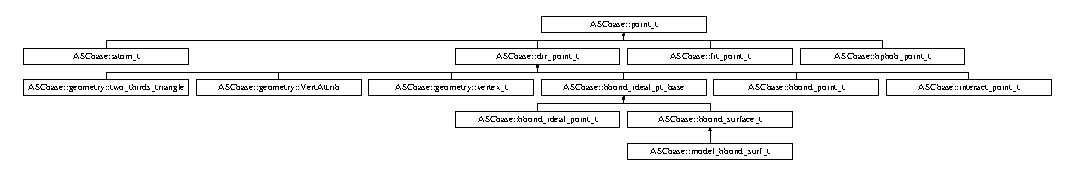
\includegraphics[height=1.92044cm]{classASCbase_1_1point__t}
\end{center}
\end{figure}
\subsection*{Public Member Functions}
\begin{CompactItemize}
\item 
\textbf{point\_\-t} (alloc\_\-t a=ALLOC\_\-POSITION)\label{classASCbase_1_1point__t_c272fe4793377a4543ccb9025a477bec}

\item 
\textbf{point\_\-t} (const \bf{point\_\-t} \&p)\label{classASCbase_1_1point__t_0e9d5784e8a556df602f789a334b4012}

\item 
const \bf{point\_\-t} \& \textbf{operator=} (const \bf{point\_\-t} \&p)\label{classASCbase_1_1point__t_d080933bfb47d744e16b8743746049df}

\item 
void \textbf{delete\_\-pos} ()\label{classASCbase_1_1point__t_7e9fb20071bf009848e2f7d195c19f49}

\end{CompactItemize}
\subsection*{Public Attributes}
\begin{CompactItemize}
\item 
my\_\-float\_\-t $\ast$ \textbf{pos}\label{classASCbase_1_1point__t_f264a8131763764aa42e9413724d95ab}

\end{CompactItemize}
\subsection*{Private Member Functions}
\begin{CompactItemize}
\item 
void \textbf{do\_\-copy} (const \bf{point\_\-t} \&p)\label{classASCbase_1_1point__t_4fb309478887055873d76b050de2f2af}

\end{CompactItemize}
\subsection*{Private Attributes}
\begin{CompactItemize}
\item 
alloc\_\-t \textbf{A\_\-mem\_\-allocated}\label{classASCbase_1_1point__t_34c86316f6870087a82770b30ba300ce}

\end{CompactItemize}


\subsection{Detailed Description}
Base class for a point that supports local allocation of position or allocation within a class such as the \doxyref{point\_\-storage}{p.}{classASCbase_1_1point__storage} class. 



The documentation for this class was generated from the following file:\begin{CompactItemize}
\item 
point.H\end{CompactItemize}

\section{ASCbase::Point\-Octree Class Reference}
\label{classASCbase_1_1PointOctree}\index{ASCbase::PointOctree@{ASCbase::PointOctree}}
Adaptive octree for the \doxyref{point\_\-t}{p.}{classASCbase_1_1point__t} datatype.  


{\tt \#include $<$Point\-Octree.H$>$}

\subsection*{Public Types}
\begin{CompactItemize}
\item 
\textbf{NO\_\-INTERSECTION} = 0\label{classASCbase_1_1PointOctree_80fe7b8c8af1229786dbaecb7ccb309061dba93a370115c369fb1a8ae073b261}

\item 
\textbf{CENTER\_\-IN\_\-CUBE}\label{classASCbase_1_1PointOctree_80fe7b8c8af1229786dbaecb7ccb30909a3c5177988c3b9dc45660468e661efe}

\item 
\textbf{POSSIBLE\_\-INTERSECTION}\label{classASCbase_1_1PointOctree_80fe7b8c8af1229786dbaecb7ccb3090f06b63246103bc5a2673ff617e5b23ba}

\item 
\textbf{CUBE\_\-AND\_\-SPHERE\_\-INTERSECT}\label{classASCbase_1_1PointOctree_80fe7b8c8af1229786dbaecb7ccb3090e080c910e2c558e73ba9da4b7dee94a8}

\item 
enum \textbf{cube\_\-sphere\_\-intersect\_\-t} \{ \textbf{NO\_\-INTERSECTION} =  0, 
\textbf{CENTER\_\-IN\_\-CUBE}, 
\textbf{POSSIBLE\_\-INTERSECTION}, 
\textbf{CUBE\_\-AND\_\-SPHERE\_\-INTERSECT}
 \}
\end{CompactItemize}
\subsection*{Public Member Functions}
\begin{CompactItemize}
\item 
\textbf{Point\-Octree} (atom\_\-vci first, atom\_\-vci last, const my\_\-float\_\-t min\_\-half\_\-width=4.5, const uint max\_\-numel=1)\label{classASCbase_1_1PointOctree_d4542cde89263eed14b44af4c3c1cabb}

\item 
void \textbf{get\_\-close\_\-points} (atom\_\-vci a, const my\_\-float\_\-t max\_\-dist, std::vector$<$ atom\_\-vci $>$ $\ast$close\_\-points)\label{classASCbase_1_1PointOctree_caf133dd6c8f3fcbbbe0835f0a0738ed}

\item 
void \textbf{get\_\-close\_\-points} (const octree\_\-node\_\-t$<$ atom\_\-vci $>$ $\ast$cnode, const my\_\-float\_\-t $\ast$pt, const my\_\-float\_\-t pt\_\-tol, std::vector$<$ atom\_\-vci $>$ $\ast$close\_\-points, int level)\label{classASCbase_1_1PointOctree_882dc85ada0fa27226db94d2a84f8caa}

\item 
void \textbf{bin\_\-trace} ()\label{classASCbase_1_1PointOctree_2a852ae8875370f5a3addd9ef4931770}

\end{CompactItemize}
\subsection*{Private Member Functions}
\begin{CompactItemize}
\item 
void \textbf{build} (atom\_\-vci first, atom\_\-vci last)\label{classASCbase_1_1PointOctree_16d33c6f4d05a3fbb19d39ab6d70e342}

\item 
void \textbf{subdivide} (octree\_\-node\_\-t$<$ atom\_\-vci $>$ $\ast$cnode)\label{classASCbase_1_1PointOctree_8dbe0c4bb2a2914528f0cf9f66b08f59}

\item 
void \bf{free\_\-octree\_\-node} (octree\_\-node\_\-t$<$ atom\_\-vci $>$ $\ast$cnode)
\item 
cube\_\-sphere\_\-intersect\_\-t \textbf{point\_\-in\_\-cube} (const my\_\-float\_\-t $\ast$centroid, const my\_\-float\_\-t half\_\-width, const my\_\-float\_\-t $\ast$pt, const my\_\-float\_\-t radius)\label{classASCbase_1_1PointOctree_b3569e8b1ea100a74666ce00b0a7278f}

\item 
cube\_\-sphere\_\-intersect\_\-t \textbf{cube\_\-and\_\-sphere\_\-intersect} (const my\_\-float\_\-t $\ast$centroid, const my\_\-float\_\-t half\_\-width, const my\_\-float\_\-t $\ast$center, const my\_\-float\_\-t radius)\label{classASCbase_1_1PointOctree_1636cdd524d21fb60ad80b69ae78b042}

\item 
void \textbf{print\_\-bin\_\-trace} (const octree\_\-node\_\-t$<$ atom\_\-vci $>$ $\ast$cnode, int level)\label{classASCbase_1_1PointOctree_39e097047618b2c80bb6ea1f9e7a74a9}

\item 
bool \textbf{line\_\-in\_\-sphere} (const my\_\-float\_\-t $\ast$centroid, const my\_\-float\_\-t half\_\-width, const my\_\-float\_\-t $\ast$center, const my\_\-float\_\-t radius, const int idx, const my\_\-float\_\-t $\ast$sign)\label{classASCbase_1_1PointOctree_569358659a96ecc1de157cf5b4a9ddc1}

\end{CompactItemize}
\subsection*{Private Attributes}
\begin{CompactItemize}
\item 
octree\_\-node\_\-t$<$ atom\_\-vci $>$ \bf{A\_\-root}\label{classASCbase_1_1PointOctree_cf433700d8979b8a5531af09c1a722a5}

\begin{CompactList}\small\item\em Root node of the tree. \item\end{CompactList}\item 
uint \bf{A\_\-max\_\-numel}\label{classASCbase_1_1PointOctree_0e341947fdbf0da8c6507d6461c8ffe5}

\begin{CompactList}\small\item\em Max number of elements in a cube at a level less than the max level. \item\end{CompactList}\item 
my\_\-float\_\-t \bf{A\_\-min\_\-half\_\-width}\label{classASCbase_1_1PointOctree_ea82427ff395714332d21ff1ceac2716}

\begin{CompactList}\small\item\em Smallest cube should be about this size. \item\end{CompactList}\end{CompactItemize}
\subsection*{Static Private Attributes}
\begin{CompactItemize}
\item 
static const std::string \bf{A\_\-fname}\label{classASCbase_1_1PointOctree_6b1e10ac2fe83f68cc03bdd24ec8d9ca}

\begin{CompactList}\small\item\em Name of the source file. \item\end{CompactList}\end{CompactItemize}


\subsection{Detailed Description}
Adaptive octree for the \doxyref{point\_\-t}{p.}{classASCbase_1_1point__t} datatype. 

It is reasonably efficient when compared with brute force, but a few more checks and the number of returned points, etc would be reduced further. 



\subsection{Member Function Documentation}
\index{ASCbase::PointOctree@{ASCbase::Point\-Octree}!free_octree_node@{free\_\-octree\_\-node}}
\index{free_octree_node@{free\_\-octree\_\-node}!ASCbase::PointOctree@{ASCbase::Point\-Octree}}
\subsubsection{\setlength{\rightskip}{0pt plus 5cm}void ASCbase::Point\-Octree::free\_\-octree\_\-node (octree\_\-node\_\-t$<$ atom\_\-vci $>$ $\ast$ {\em cnode})\hspace{0.3cm}{\tt  [inline, private]}}\label{classASCbase_1_1PointOctree_312dabdbfa0177cf2336fe534032b811}


This function was not tested enough and it should also be timed to check if it is really any faster than near\_\-by\_\-points for each point 

The documentation for this class was generated from the following file:\begin{CompactItemize}
\item 
Point\-Octree.H\end{CompactItemize}

\section{ASCbase::pos\_\-dep\_\-on\_\-joints Class Reference}
\label{classASCbase_1_1pos__dep__on__joints}\index{ASCbase::pos_dep_on_joints@{ASCbase::pos\_\-dep\_\-on\_\-joints}}
A simple data class for a block of a block matrix.  


{\tt \#include $<$Surf\-Deps\-Joints.H$>$}

\subsection*{Public Member Functions}
\begin{CompactItemize}
\item 
\textbf{pos\_\-dep\_\-on\_\-joints} (const \bf{pos\_\-dep\_\-on\_\-joints} \&other)\label{classASCbase_1_1pos__dep__on__joints_a4d2e825eaa2ae2553a8d7f2d66ed89f}

\item 
const \bf{pos\_\-dep\_\-on\_\-joints} \& \textbf{operator=} (const \bf{pos\_\-dep\_\-on\_\-joints} \&other)\label{classASCbase_1_1pos__dep__on__joints_39042623fb7f7515fcd7d32bd90650d7}

\item 
my\_\-float\_\-t $\ast$ \textbf{mutable\_\-J\_\-block} ()\label{classASCbase_1_1pos__dep__on__joints_85b245396b5836c8d29c4416fbea415e}

\item 
const my\_\-float\_\-t $\ast$ \textbf{J\_\-block} () const \label{classASCbase_1_1pos__dep__on__joints_9ee419794ff9722634571b40d782db0b}

\item 
my\_\-float\_\-t $\ast$ \textbf{mutable\_\-pinv\_\-Jtrans\_\-block} ()\label{classASCbase_1_1pos__dep__on__joints_3fca56953be29994e0ccbdbfbbc10e3d}

\item 
const my\_\-float\_\-t $\ast$ \textbf{pinv\_\-Jtrans\_\-block} () const \label{classASCbase_1_1pos__dep__on__joints_872dca61f0aab268dc6e1e6410839d4f}

\item 
void \textbf{set\_\-nrows} (size\_\-t nrows\_\-in)\label{classASCbase_1_1pos__dep__on__joints_8f0c3af5f80ff453a25725814fe066fb}

\item 
const size\_\-t \textbf{nrows} () const \label{classASCbase_1_1pos__dep__on__joints_cd80bf7a3eec0bf71a98096e781ea4f3}

\item 
const size\_\-t \textbf{ncols} () const \label{classASCbase_1_1pos__dep__on__joints_e7b83cb4f3741807ad2d3d18d3a54ec4}

\end{CompactItemize}
\subsection*{Public Attributes}
\begin{CompactItemize}
\item 
std::vector$<$ my\_\-float\_\-t $\ast$ $>$ \textbf{verts}\label{classASCbase_1_1pos__dep__on__joints_91721d7c401af41d94824188e80ad9f9}

\item 
std::vector$<$ my\_\-float\_\-t $\ast$ $>$ \textbf{normals}\label{classASCbase_1_1pos__dep__on__joints_f5e7d20d58cae9712b824f4cb41660b0}

\item 
std::vector$<$ int $>$ \textbf{num\_\-joints\_\-used}\label{classASCbase_1_1pos__dep__on__joints_6987ae9ce8f695eb21f9dc8d4ad7f296}

\end{CompactItemize}
\subsection*{Private Member Functions}
\begin{CompactItemize}
\item 
void \textbf{init} ()\label{classASCbase_1_1pos__dep__on__joints_904b7dd4afc1827c776ca2253c2e1add}

\item 
void \bf{do\_\-copy} (const \bf{pos\_\-dep\_\-on\_\-joints} \&other)
\begin{CompactList}\small\item\em Do a copy of the other class instance. \item\end{CompactList}\end{CompactItemize}
\subsection*{Private Attributes}
\begin{CompactItemize}
\item 
size\_\-t \textbf{A\_\-nrows}\label{classASCbase_1_1pos__dep__on__joints_ca7c5a4887e8864b3e979779014830f1}

\item 
size\_\-t \textbf{A\_\-ncols}\label{classASCbase_1_1pos__dep__on__joints_c9a33cb5cf6e0a3ca336546dc6ce0357}

\item 
my\_\-float\_\-t $\ast$ \textbf{A\_\-J\_\-block}\label{classASCbase_1_1pos__dep__on__joints_bc866573b0c3f4e4c77b67924fa40076}

\item 
my\_\-float\_\-t $\ast$ \textbf{A\_\-pinv\_\-Jtrans\_\-block}\label{classASCbase_1_1pos__dep__on__joints_800d04add909fab6d2d09bf41a298f40}

\end{CompactItemize}


\subsection{Detailed Description}
A simple data class for a block of a block matrix. 



\subsection{Member Function Documentation}
\index{ASCbase::pos_dep_on_joints@{ASCbase::pos\_\-dep\_\-on\_\-joints}!do_copy@{do\_\-copy}}
\index{do_copy@{do\_\-copy}!ASCbase::pos_dep_on_joints@{ASCbase::pos\_\-dep\_\-on\_\-joints}}
\subsubsection{\setlength{\rightskip}{0pt plus 5cm}void ASCbase::pos\_\-dep\_\-on\_\-joints::do\_\-copy (const \bf{pos\_\-dep\_\-on\_\-joints} \& {\em other})\hspace{0.3cm}{\tt  [inline, private]}}\label{classASCbase_1_1pos__dep__on__joints_ae39e679f64999ac2afd3896e7bcf2de}


Do a copy of the other class instance. 

NOTE: block is a pointer to the first entry of a block with in a large block matrix. Thus this copy does not make a deep copy of the block matrix nor the entire matrix 

The documentation for this class was generated from the following file:\begin{CompactItemize}
\item 
Surf\-Deps\-Joints.H\end{CompactItemize}

\section{ASCbase::prot\_\-joint\_\-dep Class Reference}
\label{classASCbase_1_1prot__joint__dep}\index{ASCbase::prot_joint_dep@{ASCbase::prot\_\-joint\_\-dep}}
Class to handle mobile residues -- rotatable joints for each residue.  


{\tt \#include $<$prot\_\-joint\_\-dep.H$>$}

\subsection*{Public Types}
\begin{CompactItemize}
\item 
typedef std::map$<$ atom\_\-type, std::vector$<$ atom\_\-type $>$ $>$ \textbf{joint\_\-dep\_\-tbl\_\-atom\_\-lvl}\label{classASCbase_1_1prot__joint__dep_9e36ead4cfdfc490f727f6c417480421}

\item 
typedef std::map$<$ residue\_\-type, joint\_\-dep\_\-tbl\_\-atom\_\-lvl $>$ \textbf{joint\_\-dep\_\-tbl\_\-res\_\-lvl}\label{classASCbase_1_1prot__joint__dep_ea37de1c525672bf30521e8e97282cb4}

\item 
typedef std::map$<$ residue\_\-vci, \bf{residue\_\-joints} $>$::const\_\-iterator \textbf{res\_\-to\_\-joints\_\-mci}\label{classASCbase_1_1prot__joint__dep_ff1116a39fb38afeaa53971b2b39cfa1}

\end{CompactItemize}
\subsection*{Public Member Functions}
\begin{CompactItemize}
\item 
bool \bf{add\_\-residue\_\-info} (const \bf{PDBStructure} $\ast$prot, residue\_\-vci res, const \bf{residue\_\-joints} $\ast$$\ast$j)
\begin{CompactList}\small\item\em Add mobile atoms (based on bond network not other constraints). \item\end{CompactList}\item 
res\_\-to\_\-joints\_\-mci \textbf{joints\_\-begin} () const \label{classASCbase_1_1prot__joint__dep_4c89eabdd2a06a9ad881fec55aff32d6}

\item 
res\_\-to\_\-joints\_\-mci \textbf{joints\_\-end} () const \label{classASCbase_1_1prot__joint__dep_49c901cd2d806782ed5be925e93ea72d}

\item 
const joint\_\-deps\_\-t \& \textbf{get\_\-joints\_\-info} (residue\_\-type res\_\-name)\label{classASCbase_1_1prot__joint__dep_6eb47defc3517af3de338df188ba0993}

\item 
const bool \textbf{fail} ()\label{classASCbase_1_1prot__joint__dep_ae8b48cbd3294ff3ec1b40cc637c2db0}

\end{CompactItemize}
\subsection*{Private Member Functions}
\begin{CompactItemize}
\item 
void \textbf{init} ()\label{classASCbase_1_1prot__joint__dep_4f10e02931d487269a4987cfb6408791}

\end{CompactItemize}
\subsection*{Private Attributes}
\begin{CompactItemize}
\item 
bool \textbf{A\_\-fail}\label{classASCbase_1_1prot__joint__dep_54fd130e58b3deeb5f66dc94eb02b99a}

\item 
joint\_\-dep\_\-tbl\_\-res\_\-lvl \textbf{A\_\-atoms\_\-dep\_\-on\_\-joint}\label{classASCbase_1_1prot__joint__dep_db46d04a0979968d80e81663454c2d5e}

\item 
std::vector$<$ atom\_\-type $>$ \textbf{A\_\-unknown\_\-residue\_\-vec}\label{classASCbase_1_1prot__joint__dep_5a8e3059f806f770411915200b7caddd}

\item 
std::vector$<$ atom\_\-type $>$ \textbf{A\_\-unknown\_\-atom\_\-vec}\label{classASCbase_1_1prot__joint__dep_aef12ef042d6d8a16e19265d3b17b47e}

\item 
std::map$<$ residue\_\-type, joint\_\-deps\_\-t $>$ \textbf{A\_\-res\_\-map}\label{classASCbase_1_1prot__joint__dep_970b14f7c96ce896be316d66ce1a797b}

\item 
std::map$<$ residue\_\-vci, \bf{residue\_\-joints} $>$ \bf{A\_\-joint\_\-blocks}\label{classASCbase_1_1prot__joint__dep_b28915bf49d2cb1789e3620d989daa07}

\begin{CompactList}\small\item\em Groups of consecutive rows that correspond to joints from one residue -- ordered by residue number and chain\-ID. \item\end{CompactList}\end{CompactItemize}
\subsection*{Static Private Attributes}
\begin{CompactItemize}
\item 
static const atom\_\-type \textbf{ALA\_\-atoms} [$\,$] = \{N, CA, C, O, CB\}\label{classASCbase_1_1prot__joint__dep_bdfba272e362e3aaec7a1c7a4a236413}

\item 
static const atom\_\-type \textbf{ARG\_\-atoms} [$\,$]
\item 
static const atom\_\-type \textbf{ASN\_\-atoms} [$\,$] = \{N, CA, C, O, CB, CG, OD1, ND2\}\label{classASCbase_1_1prot__joint__dep_c42be93f2786f326aa7ca4900a243568}

\item 
static const atom\_\-type \textbf{ASP\_\-atoms} [$\,$] = \{N, CA, C, O, CB, CG, OD1, OD2\}\label{classASCbase_1_1prot__joint__dep_98f917b5a699f9f048933fbec9170136}

\item 
static const atom\_\-type \textbf{CYS\_\-atoms} [$\,$] = \{N, CA, C, O, CB, SG\}\label{classASCbase_1_1prot__joint__dep_ff8c1b4fd6995e071efd57c053760338}

\item 
static const atom\_\-type \textbf{GLN\_\-atoms} [$\,$]
\item 
static const atom\_\-type \textbf{GLU\_\-atoms} [$\,$]
\item 
static const atom\_\-type \textbf{GLY\_\-atoms} [$\,$] = \{N, CA, C, O\}\label{classASCbase_1_1prot__joint__dep_388d19cb5bb2bdbc270b4b6c82b406f3}

\item 
static const atom\_\-type \textbf{HIS\_\-atoms} [$\,$]
\item 
static const atom\_\-type \textbf{ILE\_\-atoms} [$\,$] = \{N, CA, C, O, CB, CG1, CG2, CD1\}\label{classASCbase_1_1prot__joint__dep_3b3e44de9218be85c84ab92e07cd306e}

\item 
static const atom\_\-type \textbf{LEU\_\-atoms} [$\,$] = \{N, CA, C, O, CB, CG, CD1, CD2\}\label{classASCbase_1_1prot__joint__dep_d9b51ba5dbb4d4e87307d7919cd28e25}

\item 
static const atom\_\-type \textbf{LYS\_\-atoms} [$\,$] = \{N, CA, C, O, CB, CG, CD, CE, NZ\}\label{classASCbase_1_1prot__joint__dep_d85c7a75fc06cce60194df94c98a670e}

\item 
static const atom\_\-type \textbf{MET\_\-atoms} [$\,$] = \{N, CA, C, O, CB, CG, SD, CE\}\label{classASCbase_1_1prot__joint__dep_b88f61ad6c202cec8d2d4c9862d42b56}

\item 
static const atom\_\-type \textbf{PHE\_\-atoms} [$\,$]
\item 
static const atom\_\-type \textbf{PRO\_\-atoms} [$\,$] = \{N, CA, C, O, CB, CG, CD\}\label{classASCbase_1_1prot__joint__dep_a047cddbe0cb0dae3c19407fe6b5b9f8}

\item 
static const atom\_\-type \textbf{SER\_\-atoms} [$\,$] = \{N, CA, C, O, CB, OG\}\label{classASCbase_1_1prot__joint__dep_83654fa964913525ee564c1a83d3dbcf}

\item 
static const atom\_\-type \textbf{THR\_\-atoms} [$\,$] = \{N, CA, C, O, CB, OG1, CG2\}\label{classASCbase_1_1prot__joint__dep_2dc4ca2d156eb27d696d35c740bcb34e}

\item 
static const atom\_\-type \textbf{TRP\_\-atoms} [$\,$]
\item 
static const atom\_\-type \textbf{TYR\_\-atoms} [$\,$]
\item 
static const atom\_\-type \textbf{VAL\_\-atoms} [$\,$] = \{N, CA, C, O, CB, CG1, CG2\}\label{classASCbase_1_1prot__joint__dep_da6c6ceab748e553c5695344c58aefff}

\item 
static const joint\_\-deps\_\-t \textbf{ALA\_\-deps} = \{ ALA\_\-atoms, 0, 5 \}\label{classASCbase_1_1prot__joint__dep_952dbe38f8ad0b8127729d6ba84b97d7}

\item 
static const joint\_\-deps\_\-t \textbf{ARG\_\-deps} = \{ ARG\_\-atoms, 3, 11 \}\label{classASCbase_1_1prot__joint__dep_65fd4251f4a673b01a07a682cbfb1ffa}

\item 
static const joint\_\-deps\_\-t \textbf{ASN\_\-deps} = \{ ASN\_\-atoms, 2, 8 \}\label{classASCbase_1_1prot__joint__dep_08ae4d6148c80f98f5f95041a478fac8}

\item 
static const joint\_\-deps\_\-t \textbf{ASP\_\-deps} = \{ ASP\_\-atoms, 2, 8 \}\label{classASCbase_1_1prot__joint__dep_fac607dcac19d1c84d54597b95f6ec02}

\item 
static const joint\_\-deps\_\-t \textbf{CYS\_\-deps} = \{ CYS\_\-atoms, 1, 6 \}\label{classASCbase_1_1prot__joint__dep_18d22c4d1a2f061809bb89d552fcc14d}

\item 
static const joint\_\-deps\_\-t \textbf{GLN\_\-deps} = \{ GLN\_\-atoms, 3, 9 \}\label{classASCbase_1_1prot__joint__dep_4aefee35dbad6c943d8ce73ebb68b2d6}

\item 
static const joint\_\-deps\_\-t \textbf{GLU\_\-deps} = \{ GLU\_\-atoms, 3, 9 \}\label{classASCbase_1_1prot__joint__dep_9753dde7e298c1584ce0af03816b28bb}

\item 
static const joint\_\-deps\_\-t \textbf{GLY\_\-deps} = \{ GLY\_\-atoms, 0, 4 \}\label{classASCbase_1_1prot__joint__dep_99d499534c8f02f34e09069f6b25fed6}

\item 
static const joint\_\-deps\_\-t \textbf{HIS\_\-deps} = \{ HIS\_\-atoms, 2, 10 \}\label{classASCbase_1_1prot__joint__dep_18e7ac5f3c807b3070349b7074d69504}

\item 
static const joint\_\-deps\_\-t \textbf{ILE\_\-deps} = \{ ILE\_\-atoms, 2, 8 \}\label{classASCbase_1_1prot__joint__dep_c3e9e61ad80c5f1ef124520c55d0d2c3}

\item 
static const joint\_\-deps\_\-t \textbf{LEU\_\-deps} = \{ LEU\_\-atoms, 2, 8 \}\label{classASCbase_1_1prot__joint__dep_4283688178a143eb12c945d4498d4ea5}

\item 
static const joint\_\-deps\_\-t \textbf{LYS\_\-deps} = \{ LYS\_\-atoms, 4, 9 \}\label{classASCbase_1_1prot__joint__dep_e4498e5c919a95e72910c9b127b86253}

\item 
static const joint\_\-deps\_\-t \textbf{MET\_\-deps} = \{ MET\_\-atoms, 3, 8 \}\label{classASCbase_1_1prot__joint__dep_e872ffbde7c5e3b7a70ed361b3a34bdd}

\item 
static const joint\_\-deps\_\-t \textbf{PHE\_\-deps} = \{ PHE\_\-atoms, 2, 11 \}\label{classASCbase_1_1prot__joint__dep_b11dbf3a7007396f15fa2b20c477abd9}

\item 
static const joint\_\-deps\_\-t \textbf{PRO\_\-deps} = \{ PRO\_\-atoms, 0, 7 \}\label{classASCbase_1_1prot__joint__dep_b4938e30da71c81440ddd1e3ddbe69cb}

\item 
static const joint\_\-deps\_\-t \textbf{SER\_\-deps} = \{ SER\_\-atoms, 1, 6 \}\label{classASCbase_1_1prot__joint__dep_f381c853c58c15f7edf528bc97b0f433}

\item 
static const joint\_\-deps\_\-t \textbf{THR\_\-deps} = \{ THR\_\-atoms, 1, 7 \}\label{classASCbase_1_1prot__joint__dep_88aae83dea1f46fe3290472bda94d3ac}

\item 
static const joint\_\-deps\_\-t \textbf{TRP\_\-deps} = \{ TRP\_\-atoms, 2, 14 \}\label{classASCbase_1_1prot__joint__dep_6c55f10b16638027e48422d5d544dc6c}

\item 
static const joint\_\-deps\_\-t \textbf{TYR\_\-deps} = \{ TYR\_\-atoms, 2, 12 \}\label{classASCbase_1_1prot__joint__dep_3c8b12464a851cee0321652191b8fea8}

\item 
static const joint\_\-deps\_\-t \textbf{VAL\_\-deps} = \{ VAL\_\-atoms, 1, 7 \}\label{classASCbase_1_1prot__joint__dep_ccabd31547bdfb65023bff5e09bc9aaa}

\end{CompactItemize}


\subsection{Detailed Description}
Class to handle mobile residues -- rotatable joints for each residue. 

Build the data structure based using \doxyref{add\_\-residue\_\-info()}{p.}{classASCbase_1_1prot__joint__dep_a1cb25bee328bc154ca8fe35044b4c28} Get the joints using get\_\-joints() and check that the returned iterator is valid by comparing it against joints\_\-end() 



\subsection{Member Function Documentation}
\index{ASCbase::prot_joint_dep@{ASCbase::prot\_\-joint\_\-dep}!add_residue_info@{add\_\-residue\_\-info}}
\index{add_residue_info@{add\_\-residue\_\-info}!ASCbase::prot_joint_dep@{ASCbase::prot\_\-joint\_\-dep}}
\subsubsection{\setlength{\rightskip}{0pt plus 5cm}bool prot\_\-joint\_\-dep::add\_\-residue\_\-info (const \bf{PDBStructure} $\ast$ {\em prot}, residue\_\-vci {\em res}, const \bf{residue\_\-joints} $\ast$$\ast$ {\em j})}\label{classASCbase_1_1prot__joint__dep_a1cb25bee328bc154ca8fe35044b4c28}


Add mobile atoms (based on bond network not other constraints). 

Do not use this to add neighboring residues which we will hold fixed. 

\subsection{Member Data Documentation}
\index{ASCbase::prot_joint_dep@{ASCbase::prot\_\-joint\_\-dep}!ARG_atoms@{ARG\_\-atoms}}
\index{ARG_atoms@{ARG\_\-atoms}!ASCbase::prot_joint_dep@{ASCbase::prot\_\-joint\_\-dep}}
\subsubsection{\setlength{\rightskip}{0pt plus 5cm}const atom\_\-type prot\_\-joint\_\-dep::ARG\_\-atoms\hspace{0.3cm}{\tt  [static, private]}}\label{classASCbase_1_1prot__joint__dep_e9694a2c1acdb92adcceaf04b49437bd}


\textbf{Initial value:}

\begin{Code}\begin{verbatim} 
  {N, CA, C, O, CB, CG, CD, NE, CZ, NH1, NH2}
\end{verbatim}\end{Code}
\index{ASCbase::prot_joint_dep@{ASCbase::prot\_\-joint\_\-dep}!GLN_atoms@{GLN\_\-atoms}}
\index{GLN_atoms@{GLN\_\-atoms}!ASCbase::prot_joint_dep@{ASCbase::prot\_\-joint\_\-dep}}
\subsubsection{\setlength{\rightskip}{0pt plus 5cm}const atom\_\-type prot\_\-joint\_\-dep::GLN\_\-atoms\hspace{0.3cm}{\tt  [static, private]}}\label{classASCbase_1_1prot__joint__dep_778a227bc6f21f9df7ad071cb28a0fe4}


\textbf{Initial value:}

\begin{Code}\begin{verbatim} 
  {N, CA, C, O, CB, CG, CD, OE1, NE2}
\end{verbatim}\end{Code}
\index{ASCbase::prot_joint_dep@{ASCbase::prot\_\-joint\_\-dep}!GLU_atoms@{GLU\_\-atoms}}
\index{GLU_atoms@{GLU\_\-atoms}!ASCbase::prot_joint_dep@{ASCbase::prot\_\-joint\_\-dep}}
\subsubsection{\setlength{\rightskip}{0pt plus 5cm}const atom\_\-type prot\_\-joint\_\-dep::GLU\_\-atoms\hspace{0.3cm}{\tt  [static, private]}}\label{classASCbase_1_1prot__joint__dep_f126d6eee30314bf4d880970cf51c135}


\textbf{Initial value:}

\begin{Code}\begin{verbatim} 
  {N, CA, C, O, CB, CG, CD, OE1, OE2}
\end{verbatim}\end{Code}
\index{ASCbase::prot_joint_dep@{ASCbase::prot\_\-joint\_\-dep}!HIS_atoms@{HIS\_\-atoms}}
\index{HIS_atoms@{HIS\_\-atoms}!ASCbase::prot_joint_dep@{ASCbase::prot\_\-joint\_\-dep}}
\subsubsection{\setlength{\rightskip}{0pt plus 5cm}const atom\_\-type prot\_\-joint\_\-dep::HIS\_\-atoms\hspace{0.3cm}{\tt  [static, private]}}\label{classASCbase_1_1prot__joint__dep_027525d3ce56e48660760c3af223a4fa}


\textbf{Initial value:}

\begin{Code}\begin{verbatim} 
  {N, CA, C, O, CB, CG, ND1, CD2, CE1, NE2}
\end{verbatim}\end{Code}
\index{ASCbase::prot_joint_dep@{ASCbase::prot\_\-joint\_\-dep}!PHE_atoms@{PHE\_\-atoms}}
\index{PHE_atoms@{PHE\_\-atoms}!ASCbase::prot_joint_dep@{ASCbase::prot\_\-joint\_\-dep}}
\subsubsection{\setlength{\rightskip}{0pt plus 5cm}const atom\_\-type prot\_\-joint\_\-dep::PHE\_\-atoms\hspace{0.3cm}{\tt  [static, private]}}\label{classASCbase_1_1prot__joint__dep_e9f5147ed18c5265759259b4c6a4f575}


\textbf{Initial value:}

\begin{Code}\begin{verbatim} 
  {N, CA, C, O, CB, CG, CD1, CD2, CE1, CE2, CZ}
\end{verbatim}\end{Code}
\index{ASCbase::prot_joint_dep@{ASCbase::prot\_\-joint\_\-dep}!TRP_atoms@{TRP\_\-atoms}}
\index{TRP_atoms@{TRP\_\-atoms}!ASCbase::prot_joint_dep@{ASCbase::prot\_\-joint\_\-dep}}
\subsubsection{\setlength{\rightskip}{0pt plus 5cm}const atom\_\-type prot\_\-joint\_\-dep::TRP\_\-atoms\hspace{0.3cm}{\tt  [static, private]}}\label{classASCbase_1_1prot__joint__dep_195efde1d5901fe270a4be8c743e4a89}


\textbf{Initial value:}

\begin{Code}\begin{verbatim} 
  {N, CA, C, O, CB, CG, CD1, CD2, NE1, CE2, CE3, CZ2, CZ3, CH2}
\end{verbatim}\end{Code}
\index{ASCbase::prot_joint_dep@{ASCbase::prot\_\-joint\_\-dep}!TYR_atoms@{TYR\_\-atoms}}
\index{TYR_atoms@{TYR\_\-atoms}!ASCbase::prot_joint_dep@{ASCbase::prot\_\-joint\_\-dep}}
\subsubsection{\setlength{\rightskip}{0pt plus 5cm}const atom\_\-type prot\_\-joint\_\-dep::TYR\_\-atoms\hspace{0.3cm}{\tt  [static, private]}}\label{classASCbase_1_1prot__joint__dep_34a462915415a32e12a514d8ac434638}


\textbf{Initial value:}

\begin{Code}\begin{verbatim} 
  {N, CA, C, O, CB, CG, CD1, CD2, CE1, CE2, CZ, OH}
\end{verbatim}\end{Code}


The documentation for this class was generated from the following files:\begin{CompactItemize}
\item 
prot\_\-joint\_\-dep.H\item 
prot\_\-joint\_\-dep.C\end{CompactItemize}

\section{ASCbase::Prot\-Lig\-Score Class Reference}
\label{classASCbase_1_1ProtLigScore}\index{ASCbase::ProtLigScore@{ASCbase::ProtLigScore}}
{\tt \#include $<$Prot\-Lig\-Score.H$>$}

\subsection*{Public Types}
\begin{CompactItemize}
\item 
typedef std::pair$<$ atom\_\-vci, atom\_\-act\_\-class\_\-t $>$ \textbf{atom\_\-act\_\-pair}\label{classASCbase_1_1ProtLigScore_27d6d786f7b39152b361b23dd9d5bbbb}

\item 
typedef std::map$<$ atom\_\-vci, atom\_\-act\_\-class\_\-t $>$ \textbf{atom\_\-act\_\-map}\label{classASCbase_1_1ProtLigScore_ce33f05b2e4c44c586465cf372a608ec}

\item 
typedef atom\_\-act\_\-map::iterator \textbf{atom\_\-act\_\-mi}\label{classASCbase_1_1ProtLigScore_919ad4c17215dc1ca9072def5d1f6f80}

\item 
typedef atom\_\-act\_\-map::const\_\-iterator \textbf{atom\_\-act\_\-mci}\label{classASCbase_1_1ProtLigScore_bdea38e65c716d29e71ed2e4521eb36b}

\item 
\textbf{INITIAL} = 0\label{classASCbase_1_1ProtLigScore_38da0bbb70c6f5a88b37e99939fa72117efb63b928321c54411b880623ea0fb6}

\item 
\textbf{INTERFACIAL\_\-ATOM}\label{classASCbase_1_1ProtLigScore_38da0bbb70c6f5a88b37e99939fa7211500e8743a0b378fddf0d53d673a40b47}

\item 
\textbf{METAL\_\-DIRECT\_\-HBOND}\label{classASCbase_1_1ProtLigScore_38da0bbb70c6f5a88b37e99939fa7211e93fbf76a21bb4ea027750f686e0fece}

\item 
\textbf{SALT\_\-BRIDGE}\label{classASCbase_1_1ProtLigScore_38da0bbb70c6f5a88b37e99939fa72112a51642889c858139d7b520652703b81}

\item 
\textbf{DIRECT\_\-HBOND}\label{classASCbase_1_1ProtLigScore_38da0bbb70c6f5a88b37e99939fa7211803e8fc1cf125b935a73b960416972aa}

\item 
\textbf{UNSAT\_\-CHARGE}\label{classASCbase_1_1ProtLigScore_38da0bbb70c6f5a88b37e99939fa72113a2e21f3f5eb470e89630ace57fca557}

\item 
\textbf{UNSAT\_\-POLAR}\label{classASCbase_1_1ProtLigScore_38da0bbb70c6f5a88b37e99939fa721193ca1d17e498b2126dd19ebeb0f93abf}

\item 
\textbf{INTRA\_\-LIGAND\_\-HBOND}\label{classASCbase_1_1ProtLigScore_38da0bbb70c6f5a88b37e99939fa721131df05afc5bf7240b89d5a0b09b0404b}

\item 
\textbf{INTRA\_\-LIGAND\_\-SALT\_\-BRIDGE}\label{classASCbase_1_1ProtLigScore_38da0bbb70c6f5a88b37e99939fa72119f36f771a2f0c2060396f693a09097aa}

\item 
\textbf{INTRA\_\-TARGET\_\-HBOND}\label{classASCbase_1_1ProtLigScore_38da0bbb70c6f5a88b37e99939fa7211465a604ea7061692e2e210b6b5d50a72}

\item 
\textbf{INTRA\_\-TARGET\_\-SALT\_\-BRIDGE}\label{classASCbase_1_1ProtLigScore_38da0bbb70c6f5a88b37e99939fa7211a154b072dd519a883d0b7b9b5c3b1055}

\item 
enum \textbf{atom\_\-act\_\-class\_\-t} \{ \par
\textbf{INITIAL} =  0, 
\textbf{INTERFACIAL\_\-ATOM}, 
\textbf{METAL\_\-DIRECT\_\-HBOND}, 
\textbf{SALT\_\-BRIDGE}, 
\par
\textbf{DIRECT\_\-HBOND}, 
\textbf{UNSAT\_\-CHARGE}, 
\textbf{UNSAT\_\-POLAR}, 
\textbf{INTRA\_\-LIGAND\_\-HBOND}, 
\par
\textbf{INTRA\_\-LIGAND\_\-SALT\_\-BRIDGE}, 
\textbf{INTRA\_\-TARGET\_\-HBOND}, 
\textbf{INTRA\_\-TARGET\_\-SALT\_\-BRIDGE}
 \}
\end{CompactItemize}
\subsection*{Public Member Functions}
\begin{CompactItemize}
\item 
\textbf{Prot\-Lig\-Score} (\bf{PDBStructure} \&prot, \bf{mol2File} \&lig, bool save\_\-prot\_\-lig\_\-acts=true, bool compute\_\-charge\_\-sums=true)\label{classASCbase_1_1ProtLigScore_1770dc58245d85131f7040e5acffdeff}

\item 
const my\_\-float\_\-t \textbf{affiscore} () const \label{classASCbase_1_1ProtLigScore_3b141a7e5ba3c877356e268809133520}

\item 
const my\_\-float\_\-t \textbf{orientscore} () const \label{classASCbase_1_1ProtLigScore_5d08bfc7c970cb20a8418452c70f676e}

\item 
const my\_\-float\_\-t \textbf{ligand\_\-efficiency} () const \label{classASCbase_1_1ProtLigScore_1f92dc0a2b0830b392f6f5648e6e316b}

\item 
void \textbf{print\_\-hbonds} (std::ostream \&out)\label{classASCbase_1_1ProtLigScore_2632d23a6e61c4c16781bf8fe9323fda}

\item 
void \textbf{classic\_\-report} (std::ostream \&out)\label{classASCbase_1_1ProtLigScore_60120a05bc1c6cd704174e08e3110ba1}

\item 
void \textbf{report\_\-scores} (std::ostream \&out, char delim= '$|$')\label{classASCbase_1_1ProtLigScore_908635d9e01981a9e813df7947505f3d}

\item 
void \bf{gen\_\-lig\_\-act\_\-strings} (const char field\_\-delim= '$|$', const char prot\_\-delim= ',')
\begin{CompactList}\small\item\em Generate the ligand atoms' interaction strings. \item\end{CompactList}\item 
void \bf{write\_\-lig\_\-acts} (std::ostream \&out=std::cout, char field\_\-delim= '$|$', char prot\_\-delim= ',')\label{classASCbase_1_1ProtLigScore_1433bfcfed24d1a064ad4ead1f5e6a47}

\begin{CompactList}\small\item\em Write the ligand atoms with corresponding interactions from the protein. \item\end{CompactList}\item 
std::vector$<$ salt\_\-bridge\_\-t $>$::const\_\-iterator \textbf{salt\_\-bridges\_\-begin} () const \label{classASCbase_1_1ProtLigScore_91e6b0e118597d22d6a7cd4deecc45da}

\item 
std::vector$<$ salt\_\-bridge\_\-t $>$::const\_\-iterator \textbf{salt\_\-bridges\_\-end} () const \label{classASCbase_1_1ProtLigScore_ea289b8b558b201953876c8e9ed0f4a3}

\item 
std::vector$<$ hbond\_\-t $>$::const\_\-iterator \textbf{hbonds\_\-begin} () const \label{classASCbase_1_1ProtLigScore_52476c5b5fdeb1e03c06f92ab6be71e0}

\item 
std::vector$<$ hbond\_\-t $>$::const\_\-iterator \textbf{hbonds\_\-end} () const \label{classASCbase_1_1ProtLigScore_9c33162446d3ba3d1788878ffea98039}

\item 
std::map$<$ residue\_\-vci, bool $>$::const\_\-iterator \textbf{hphob\_\-SC\_\-begin} () const \label{classASCbase_1_1ProtLigScore_78531873dda937cd13058da1898dc9b9}

\item 
std::map$<$ residue\_\-vci, bool $>$::const\_\-iterator \textbf{hphob\_\-SC\_\-end} () const \label{classASCbase_1_1ProtLigScore_2450c044ac7c187dd0cf1a74fd3f15ad}

\item 
const std::string \textbf{lig\_\-name} () const \label{classASCbase_1_1ProtLigScore_c17dbe0c860a1d3f6b43c6e82eade318}

\item 
std::vector$<$ std::string $>$::const\_\-iterator \bf{lig\_\-act\_\-strings\_\-begin} ()
\item 
std::vector$<$ std::string $>$::const\_\-iterator \bf{lig\_\-act\_\-strings\_\-end} ()
\end{CompactItemize}
\subsection*{Static Public Member Functions}
\begin{CompactItemize}
\item 
static void \textbf{score\_\-header\_\-lines} (std::ostream \&out, bool classic=false)\label{classASCbase_1_1ProtLigScore_dc5ffb2f1b082529473e3ee6f2843ba8}

\end{CompactItemize}
\subsection*{Private Member Functions}
\begin{CompactItemize}
\item 
void \textbf{compute\_\-scores} ()\label{classASCbase_1_1ProtLigScore_020f3f7d5ed48200fee48009a7bd0981}

\item 
void \textbf{compute\_\-terms} ()\label{classASCbase_1_1ProtLigScore_3273df40e4af4de8771f42a171ff49b9}

\item 
void \textbf{metal\_\-interactions} (atom\_\-vci lig\_\-atom, int $\ast$num\_\-lig\_\-nbrs)\label{classASCbase_1_1ProtLigScore_43197dcbdb8db5e8134c4536593a1554}

\item 
void \textbf{prot\_\-lig\_\-atom\_\-interactions} (atom\_\-vci lig\_\-atom, int $\ast$num\_\-lig\_\-nbrs, int $\ast$sum\_\-hphob\_\-hphob, int $\ast$num\_\-hphob\_\-hphob\_\-contact\_\-1\_\-lig\_\-atm)\label{classASCbase_1_1ProtLigScore_35a77eb830e6ea30f0f7e0974337e507}

\item 
void \textbf{polar\_\-interaction} (atom\_\-vci prot\_\-atom, atom\_\-vci lig\_\-atom, my\_\-float\_\-t sq\_\-dist)\label{classASCbase_1_1ProtLigScore_f0ffc28a9f7912538c6a50ddbd892af3}

\item 
void \textbf{flag\_\-intra\_\-ligand\_\-hbonds} ()\label{classASCbase_1_1ProtLigScore_52feb68979289cc9695aaf867c54694e}

\item 
void \textbf{flag\_\-intra\_\-protein\_\-hbonds} ()\label{classASCbase_1_1ProtLigScore_9bf29dd817db457447811f73f49e3dff}

\item 
void \textbf{sum\_\-target\_\-hydrophobicity} ()\label{classASCbase_1_1ProtLigScore_15510c6a4dd67ed6855d344a4ea26806}

\item 
void \textbf{flag\_\-unsat\_\-polar\_\-atoms} (atom\_\-act\_\-map $\ast$my\_\-map, int $\ast$num\_\-unsat\_\-charge, int $\ast$num\_\-unsat\_\-polar)\label{classASCbase_1_1ProtLigScore_d98d4a8ed3743a00db0f83efe90d0f1e}

\item 
void \textbf{print\_\-atom\_\-act\_\-classes} (atom\_\-act\_\-map $\ast$my\_\-map)\label{classASCbase_1_1ProtLigScore_b56c70e1c49a08b5b8bd3b52b508b43d}

\end{CompactItemize}
\subsection*{Private Attributes}
\begin{CompactItemize}
\item 
\bf{PDBStructure} $\ast$ \bf{A\_\-prot}\label{classASCbase_1_1ProtLigScore_5b1a480b3bf5f9c011497ba534fa9461}

\begin{CompactList}\small\item\em Pointer to target protein data structures -- only valid while constructor is active. \item\end{CompactList}\item 
\bf{mol2File} $\ast$ \bf{A\_\-lig}\label{classASCbase_1_1ProtLigScore_dfbf1284c9cbed4b54206df9fdddef28}

\begin{CompactList}\small\item\em Pointer to ligand to score -- only valid while constructor is active. \item\end{CompactList}\item 
\bf{Hbond\-Geometry} \bf{A\_\-hbond\_\-geometry}\label{classASCbase_1_1ProtLigScore_6671697549e83639b589b71488f550d9}

\begin{CompactList}\small\item\em Instance of hbond geometry class. \item\end{CompactList}\item 
std::map$<$ atom\_\-vci, atom\_\-act\_\-class\_\-t $>$ \textbf{A\_\-ligand\_\-flag}\label{classASCbase_1_1ProtLigScore_8b4747bab4ae82a169058b0aef3a2f42}

\item 
std::map$<$ atom\_\-vci, atom\_\-act\_\-class\_\-t $>$ \textbf{A\_\-target\_\-flag}\label{classASCbase_1_1ProtLigScore_8f73fb747d5bf69e796cccad62f2926b}

\item 
std::vector$<$ salt\_\-bridge\_\-t $>$ \bf{A\_\-prot\_\-lig\_\-SB}\label{classASCbase_1_1ProtLigScore_0d045558a8b159755a49bfa691ea3977}

\begin{CompactList}\small\item\em Protein-ligand salt bridges. \item\end{CompactList}\item 
std::vector$<$ hbond\_\-t $>$ \bf{A\_\-prot\_\-lig\_\-hbonds}\label{classASCbase_1_1ProtLigScore_3cbb26774378dac3641e3060cc3bca30}

\begin{CompactList}\small\item\em Protein-ligand hbonds. \item\end{CompactList}\item 
std::map$<$ residue\_\-vci, bool $>$ \bf{A\_\-hphob\_\-prot\_\-SC}\label{classASCbase_1_1ProtLigScore_d821097b1cb76b5bcc2e784d923c64f1}

\begin{CompactList}\small\item\em Keep note of hphob sidechains interating with ligand hphob atoms. \item\end{CompactList}\item 
raw\_\-terms\_\-type \textbf{A\_\-raw\_\-terms}\label{classASCbase_1_1ProtLigScore_6057aed97ad9d2f821e0243d0e991824}

\item 
int \bf{A\_\-num\_\-lig\_\-carbons}\label{classASCbase_1_1ProtLigScore_e8f1ebf48410e8bfa049bf7dad668351}

\begin{CompactList}\small\item\em Count of carbons in the ligand. \item\end{CompactList}\item 
int \bf{A\_\-num\_\-exposed\_\-lig\_\-carbons}\label{classASCbase_1_1ProtLigScore_6886d65b0975f0c237500478ba4a198c}

\begin{CompactList}\small\item\em Count of ligand carbon atoms with no protein neighbors (within 4.5 (A)). \item\end{CompactList}\item 
std::vector$<$ my\_\-float\_\-t $>$ \textbf{A\_\-affi\_\-terms}\label{classASCbase_1_1ProtLigScore_73c73cd82b0d7bfff4838314cd84ab0b}

\item 
my\_\-float\_\-t \textbf{A\_\-affiscore}\label{classASCbase_1_1ProtLigScore_7e1e577116eee25a76c19f55682c1558}

\item 
my\_\-float\_\-t \textbf{A\_\-orientscore}\label{classASCbase_1_1ProtLigScore_5535061a8d607e195cfc72d8836e5302}

\item 
my\_\-float\_\-t \textbf{A\_\-affiefficientscore}\label{classASCbase_1_1ProtLigScore_49bb696b0e08da39348198573860b0d7}

\item 
bool \textbf{A\_\-keep\_\-prot\_\-lig\_\-acts}\label{classASCbase_1_1ProtLigScore_bbc85c49bf05b6d54a1f786596f47b1f}

\item 
std::vector$<$ std::vector$<$ residue\_\-vci $>$ $>$ \textbf{A\_\-hphob\_\-prot\_\-lig\_\-SC}\label{classASCbase_1_1ProtLigScore_f737fa004d7fa88be1f6f9c6d155b099}

\item 
std::vector$<$ bool $>$ \textbf{A\_\-lig\_\-exposed\_\-Cz}\label{classASCbase_1_1ProtLigScore_c449cc6743b06bef1df97a236a693305}

\item 
std::vector$<$ std::string $>$ \bf{A\_\-lig\_\-act\_\-strings}\label{classASCbase_1_1ProtLigScore_615545947d1470e69c9aa7b0169b4b28}

\begin{CompactList}\small\item\em A string for each ligand atom that denoting interactions with the protein. \item\end{CompactList}\end{CompactItemize}
\subsection*{Static Private Attributes}
\begin{CompactItemize}
\item 
static const my\_\-float\_\-t \textbf{MIN\_\-BURY\_\-SQUARED\_\-DIST} = 1.9 $\ast$ 1.9\label{classASCbase_1_1ProtLigScore_f5458d92783fb455d0a7b474734862ac}

\item 
static const my\_\-float\_\-t \textbf{MAX\_\-BURY\_\-SQUARED\_\-DIST} = 4.5 $\ast$ 4.5\label{classASCbase_1_1ProtLigScore_8351bdb8162c375a142cc69d4125661a}

\item 
static const my\_\-float\_\-t \textbf{HYDRO\_\-SQUARED\_\-DIST} = 4.5 $\ast$ 4.5\label{classASCbase_1_1ProtLigScore_9629a637153e69bc93198e76bd054ff8}

\item 
static const my\_\-float\_\-t \textbf{MAX\_\-INTERACT\_\-SQUARED\_\-DIST} = 4.5 $\ast$ 4.5\label{classASCbase_1_1ProtLigScore_38fd929f2c9ae78cc55b55383e910fa4}

\item 
static const my\_\-float\_\-t \textbf{AFFI\_\-64\_\-WEIGHTS} [$\,$]
\item 
static const my\_\-float\_\-t \textbf{ORIENT\_\-99\_\-WEIGHTS} [$\,$]
\end{CompactItemize}
\subsection*{Classes}
\begin{CompactItemize}
\item 
struct \textbf{hbond\_\-t}
\item 
struct \textbf{raw\_\-terms\_\-type}
\item 
struct \textbf{salt\_\-bridge\_\-t}
\end{CompactItemize}


\subsection{Detailed Description}
Compute orientation and affinity scores between protein atoms and ligand atoms. Note: because the protein and ligand are required for scoring but also used by other functions, this class is really only valid if both the ligand and protein objects are still in scope (exist). 



\subsection{Member Function Documentation}
\index{ASCbase::ProtLigScore@{ASCbase::Prot\-Lig\-Score}!gen_lig_act_strings@{gen\_\-lig\_\-act\_\-strings}}
\index{gen_lig_act_strings@{gen\_\-lig\_\-act\_\-strings}!ASCbase::ProtLigScore@{ASCbase::Prot\-Lig\-Score}}
\subsubsection{\setlength{\rightskip}{0pt plus 5cm}void Prot\-Lig\-Score::gen\_\-lig\_\-act\_\-strings (const char {\em field\_\-delim} = {\tt '$|$'}, const char {\em prot\_\-delim} = {\tt ','})}\label{classASCbase_1_1ProtLigScore_f89729aba4e721e341a91e795438a129}


Generate the ligand atoms' interaction strings. 

This function is public to support the ASCbase\-Py interface \index{ASCbase::ProtLigScore@{ASCbase::Prot\-Lig\-Score}!lig_act_strings_begin@{lig\_\-act\_\-strings\_\-begin}}
\index{lig_act_strings_begin@{lig\_\-act\_\-strings\_\-begin}!ASCbase::ProtLigScore@{ASCbase::Prot\-Lig\-Score}}
\subsubsection{\setlength{\rightskip}{0pt plus 5cm}std::vector$<$std::string$>$::const\_\-iterator ASCbase::Prot\-Lig\-Score::lig\_\-act\_\-strings\_\-begin ()\hspace{0.3cm}{\tt  [inline]}}\label{classASCbase_1_1ProtLigScore_8b4e7de39e5853938e31039394322b4f}


Added for ASCbase\-Py interface -- why compute it in python when it is already computed and debugged in C++ \index{ASCbase::ProtLigScore@{ASCbase::Prot\-Lig\-Score}!lig_act_strings_end@{lig\_\-act\_\-strings\_\-end}}
\index{lig_act_strings_end@{lig\_\-act\_\-strings\_\-end}!ASCbase::ProtLigScore@{ASCbase::Prot\-Lig\-Score}}
\subsubsection{\setlength{\rightskip}{0pt plus 5cm}std::vector$<$std::string$>$::const\_\-iterator ASCbase::Prot\-Lig\-Score::lig\_\-act\_\-strings\_\-end ()\hspace{0.3cm}{\tt  [inline]}}\label{classASCbase_1_1ProtLigScore_934c0d6ca9955e06c2548020e415a1e9}


Added for ASCbase\-Py interface -- why compute it in python when it is already computed and debugged in C++ 

\subsection{Member Data Documentation}
\index{ASCbase::ProtLigScore@{ASCbase::Prot\-Lig\-Score}!AFFI_64_WEIGHTS@{AFFI\_\-64\_\-WEIGHTS}}
\index{AFFI_64_WEIGHTS@{AFFI\_\-64\_\-WEIGHTS}!ASCbase::ProtLigScore@{ASCbase::Prot\-Lig\-Score}}
\subsubsection{\setlength{\rightskip}{0pt plus 5cm}const my\_\-float\_\-t Prot\-Lig\-Score::AFFI\_\-64\_\-WEIGHTS\hspace{0.3cm}{\tt  [static, private]}}\label{classASCbase_1_1ProtLigScore_fed52d2f3a0f38d69cb8cfd172a0798e}


\textbf{Initial value:}

\begin{Code}\begin{verbatim} 
  {-5.218,-0.239,-0.083, 0.134,0.000,0.000,0.000 }
\end{verbatim}\end{Code}
\index{ASCbase::ProtLigScore@{ASCbase::Prot\-Lig\-Score}!ORIENT_99_WEIGHTS@{ORIENT\_\-99\_\-WEIGHTS}}
\index{ORIENT_99_WEIGHTS@{ORIENT\_\-99\_\-WEIGHTS}!ASCbase::ProtLigScore@{ASCbase::Prot\-Lig\-Score}}
\subsubsection{\setlength{\rightskip}{0pt plus 5cm}const my\_\-float\_\-t Prot\-Lig\-Score::ORIENT\_\-99\_\-WEIGHTS\hspace{0.3cm}{\tt  [static, private]}}\label{classASCbase_1_1ProtLigScore_d03935e16ddc38eacaaad7939c38c030}


\textbf{Initial value:}

\begin{Code}\begin{verbatim} 
  {-3.917,-0.061,-0.023,-0.189,0.000,0.000,0.000 }
\end{verbatim}\end{Code}


The documentation for this class was generated from the following files:\begin{CompactItemize}
\item 
Prot\-Lig\-Score.H\item 
Prot\-Lig\-Score.C\end{CompactItemize}

\section{ASCbase::Prot\-Lig\-Score\-Parameters Class Reference}
\label{classASCbase_1_1ProtLigScoreParameters}\index{ASCbase::ProtLigScoreParameters@{ASCbase::ProtLigScoreParameters}}
{\tt \#include $<$Prot\-Lig\-Score\-Parameters.H$>$}

Inheritance diagram for ASCbase::Prot\-Lig\-Score\-Parameters::\begin{figure}[H]
\begin{center}
\leavevmode
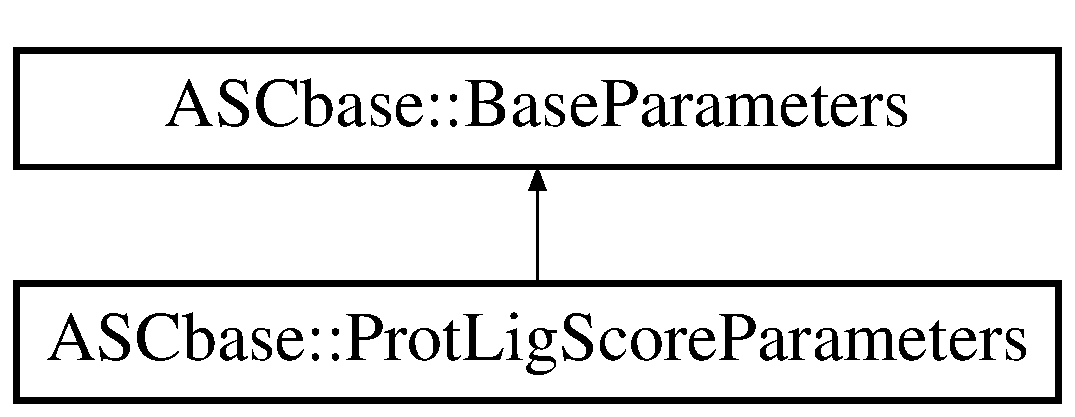
\includegraphics[height=2cm]{classASCbase_1_1ProtLigScoreParameters}
\end{center}
\end{figure}
\subsection*{Public Types}
\begin{CompactItemize}
\item 
\textbf{PRINT\_\-VERSION} = 1\label{classASCbase_1_1ProtLigScoreParameters_b7a9a2b023394c378461bd68df038bd29305d63d54f96f7ee778ef05392a7dab}

\item 
\textbf{PRINT\_\-HELP}\label{classASCbase_1_1ProtLigScoreParameters_b7a9a2b023394c378461bd68df038bd21075878cd4751c0b277fd4bc7d447435}

\item 
\textbf{BUILD\_\-INTERACTIONS\_\-TABLE}\label{classASCbase_1_1ProtLigScoreParameters_b7a9a2b023394c378461bd68df038bd291556765acaf9b14a740324aa7f42dcc}

\item 
\textbf{PRINT\_\-INTERACTIONS}\label{classASCbase_1_1ProtLigScoreParameters_b7a9a2b023394c378461bd68df038bd2fe1c72651287d18338539baf44f75cc8}

\item 
enum \textbf{popt\_\-args\_\-t} \{ \textbf{PRINT\_\-VERSION} =  1, 
\textbf{PRINT\_\-HELP}, 
\textbf{BUILD\_\-INTERACTIONS\_\-TABLE}, 
\textbf{PRINT\_\-INTERACTIONS}
 \}
\end{CompactItemize}
\subsection*{Public Member Functions}
\begin{CompactItemize}
\item 
\bf{Prot\-Lig\-Score\-Parameters} ()\label{classASCbase_1_1ProtLigScoreParameters_1d7c25c9061b1997ec8774cab0fe6ce5}

\begin{CompactList}\small\item\em To be used by the ASCbase\-Py score.parameters module. \item\end{CompactList}\item 
\bf{Prot\-Lig\-Score\-Parameters} (const int argc, const char $\ast$$\ast$argv)\label{classASCbase_1_1ProtLigScoreParameters_f8279eb37256fd5b6433900ac1ca8cab}

\begin{CompactList}\small\item\em Set the score parameters using the values in argv. \item\end{CompactList}\end{CompactItemize}
\subsection*{Public Attributes}
\begin{CompactItemize}
\item 
std::string \textbf{prot\_\-fname}\label{classASCbase_1_1ProtLigScoreParameters_d73e199c8788c4f367b7c0a246e00223}

\item 
std::string \textbf{lig\_\-fname}\label{classASCbase_1_1ProtLigScoreParameters_c6f884bad30d7e98f0fb5245dbd4d93e}

\item 
std::string \textbf{lig\_\-list\_\-fname}\label{classASCbase_1_1ProtLigScoreParameters_98f587548a6a1561b9291bfc778d5085}

\item 
bool \textbf{build\_\-interact\_\-tbl}\label{classASCbase_1_1ProtLigScoreParameters_20387a9ca9a836688d34d4e68c009632}

\item 
bool \textbf{print\_\-interactions}\label{classASCbase_1_1ProtLigScoreParameters_6d07515b95e1a858c129c8d2e6e1b5ea}

\end{CompactItemize}
\subsection*{Private Member Functions}
\begin{CompactItemize}
\item 
void \bf{init} ()
\item 
status\_\-t \bf{get\_\-opts} (const int argc, const char $\ast$$\ast$argv)
\begin{CompactList}\small\item\em Given the command line arguments, parse them using the popt library. \item\end{CompactList}\item 
status\_\-t \bf{verify\_\-parameters} ()
\begin{CompactList}\small\item\em Simple verification of command line parameters. \item\end{CompactList}\end{CompactItemize}
\subsection*{Static Private Attributes}
\begin{CompactItemize}
\item 
static const std::string \bf{A\_\-fname} = \char`\"{}Prot\-Lig\-Score\-Parameters.C\char`\"{}\label{classASCbase_1_1ProtLigScoreParameters_fa12c92a4a3e4952fd98edace796988a}

\begin{CompactList}\small\item\em Name of source file. \item\end{CompactList}\end{CompactItemize}


\subsection{Detailed Description}
A data class (public members) used to hide the details, from the main application source, needed to get the parameters. 



\subsection{Member Function Documentation}
\index{ASCbase::ProtLigScoreParameters@{ASCbase::Prot\-Lig\-Score\-Parameters}!get_opts@{get\_\-opts}}
\index{get_opts@{get\_\-opts}!ASCbase::ProtLigScoreParameters@{ASCbase::Prot\-Lig\-Score\-Parameters}}
\subsubsection{\setlength{\rightskip}{0pt plus 5cm}Base\-Parameters::status\_\-t Prot\-Lig\-Score\-Parameters::get\_\-opts (const int {\em argc}, const char $\ast$$\ast$ {\em argv})\hspace{0.3cm}{\tt  [private]}}\label{classASCbase_1_1ProtLigScoreParameters_586a96295f8218894484a4e67a903ece}


Given the command line arguments, parse them using the popt library. 

\begin{Desc}
\item[Parameters:]
\begin{description}
\item[{\em argc}]Number of command line arguments \item[{\em argv}]Array of C-style strings holding the command line arguments \end{description}
\end{Desc}
\begin{Desc}
\item[Returns:]True if parsed successfully and may continue, else false \end{Desc}
\index{ASCbase::ProtLigScoreParameters@{ASCbase::Prot\-Lig\-Score\-Parameters}!init@{init}}
\index{init@{init}!ASCbase::ProtLigScoreParameters@{ASCbase::Prot\-Lig\-Score\-Parameters}}
\subsubsection{\setlength{\rightskip}{0pt plus 5cm}void Prot\-Lig\-Score\-Parameters::init ()\hspace{0.3cm}{\tt  [private]}}\label{classASCbase_1_1ProtLigScoreParameters_71e62166bebd8b6192f7910fe3e30acb}


Initialize the class variables to standard nondefined values (such as NULL). \index{ASCbase::ProtLigScoreParameters@{ASCbase::Prot\-Lig\-Score\-Parameters}!verify_parameters@{verify\_\-parameters}}
\index{verify_parameters@{verify\_\-parameters}!ASCbase::ProtLigScoreParameters@{ASCbase::Prot\-Lig\-Score\-Parameters}}
\subsubsection{\setlength{\rightskip}{0pt plus 5cm}Base\-Parameters::status\_\-t Prot\-Lig\-Score\-Parameters::verify\_\-parameters ()\hspace{0.3cm}{\tt  [private]}}\label{classASCbase_1_1ProtLigScoreParameters_84006aef52335c65ce3c9e41eca9282d}


Simple verification of command line parameters. 

\begin{Desc}
\item[Returns:]False implies unsafe to proceed, otherwise should be OK \end{Desc}


The documentation for this class was generated from the following files:\begin{CompactItemize}
\item 
Prot\-Lig\-Score\-Parameters.H\item 
Prot\-Lig\-Score\-Parameters.C\end{CompactItemize}

\section{ASCbase::Psuedo\-Lig\-Rmsd Class Reference}
\label{classASCbase_1_1PsuedoLigRmsd}\index{ASCbase::PsuedoLigRmsd@{ASCbase::PsuedoLigRmsd}}
{\tt \#include $<$Psuedo\-Lig\-Rmsd.H$>$}

Inheritance diagram for ASCbase::Psuedo\-Lig\-Rmsd::\begin{figure}[H]
\begin{center}
\leavevmode
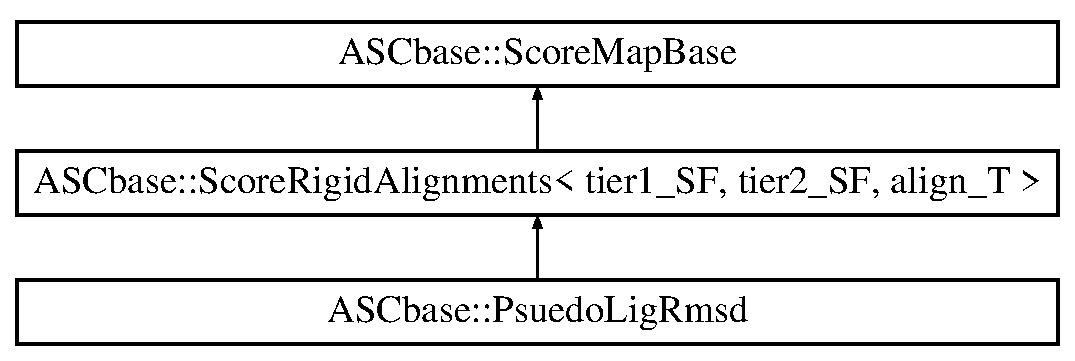
\includegraphics[height=3cm]{classASCbase_1_1PsuedoLigRmsd}
\end{center}
\end{figure}
\subsection*{Public Member Functions}
\begin{CompactItemize}
\item 
\bf{Psuedo\-Lig\-Rmsd} (\bf{Model\-Sitemap} $\ast$model\_\-in, const \bf{Search\-Parameters} \&params)\label{classASCbase_1_1PsuedoLigRmsd_cb2260f005103d3160c017839c4bd06e}

\begin{CompactList}\small\item\em Loads the model ligand and calls base cstr. \item\end{CompactList}\item 
\bf{$\sim$Psuedo\-Lig\-Rmsd} ()\label{classASCbase_1_1PsuedoLigRmsd_2ab21999e1e371a9eaa2839251d15d12}

\begin{CompactList}\small\item\em basic destruction \item\end{CompactList}\end{CompactItemize}
\subsection*{Protected Member Functions}
\begin{CompactItemize}
\item 
my\_\-float\_\-t \bf{score} (const \bf{Dbase\-Sitemap} \&search, rigid\_\-align\_\-vi scores)
\begin{CompactList}\small\item\em Given an alignment of search to the query, score said alignment. \item\end{CompactList}\item 
my\_\-float\_\-t \textbf{correspondences} (my\_\-float\_\-t $\ast$$\ast$query\_\-pts\_\-ptr, my\_\-float\_\-t $\ast$$\ast$db\_\-pts\_\-ptr, size\_\-t $\ast$npts)\label{classASCbase_1_1PsuedoLigRmsd_69e79ac94abe9233c291ecaccc6cae2e}

\end{CompactItemize}
\subsection*{Private Attributes}
\begin{CompactItemize}
\item 
\bf{mol2File} $\ast$ \textbf{model\_\-lig}\label{classASCbase_1_1PsuedoLigRmsd_c2c74580d19f2a232ad85eec12641ebe}

\end{CompactItemize}
\subsection*{Static Private Attributes}
\begin{CompactItemize}
\item 
static const std::string \bf{\_\-fname} = \char`\"{}Psuedo\-Lig\-Rmsd.C\char`\"{}\label{classASCbase_1_1PsuedoLigRmsd_2f21de3bff3a23947a0f443dd906c0bc}

\begin{CompactList}\small\item\em \char`\"{}Psuedo\-Lig\-Rmsd.C\char`\"{} \item\end{CompactList}\end{CompactItemize}


\subsection{Detailed Description}
NOTE: this method only works for ligands which are EXACTLY the same. That is the corresponding atom for the nth query ligand atom is the nth target ligand atom. 



\subsection{Member Function Documentation}
\index{ASCbase::PsuedoLigRmsd@{ASCbase::Psuedo\-Lig\-Rmsd}!score@{score}}
\index{score@{score}!ASCbase::PsuedoLigRmsd@{ASCbase::Psuedo\-Lig\-Rmsd}}
\subsubsection{\setlength{\rightskip}{0pt plus 5cm}my\_\-float\_\-t Psuedo\-Lig\-Rmsd::score (const \bf{Dbase\-Sitemap} \& {\em search}, rigid\_\-align\_\-vi {\em scores})\hspace{0.3cm}{\tt  [protected]}}\label{classASCbase_1_1PsuedoLigRmsd_889f9461ef48612a4d146c4b7c34b46c}


Given an alignment of search to the query, score said alignment. 

\begin{Desc}
\item[Parameters:]
\begin{description}
\item[{\em search}]Pointer to the sitemap aligned to the model sitemap \end{description}
\end{Desc}
\begin{Desc}
\item[Returns:]The score of the alignment \end{Desc}


The documentation for this class was generated from the following files:\begin{CompactItemize}
\item 
Psuedo\-Lig\-Rmsd.H\item 
Psuedo\-Lig\-Rmsd.C\end{CompactItemize}

\section{ASCbase::Rectangular\-Solid Class Reference}
\label{classASCbase_1_1RectangularSolid}\index{ASCbase::RectangularSolid@{ASCbase::RectangularSolid}}
A rectangular bounding volume.  


{\tt \#include $<$Bounding\-Volume.H$>$}

Inheritance diagram for ASCbase::Rectangular\-Solid::\begin{figure}[H]
\begin{center}
\leavevmode
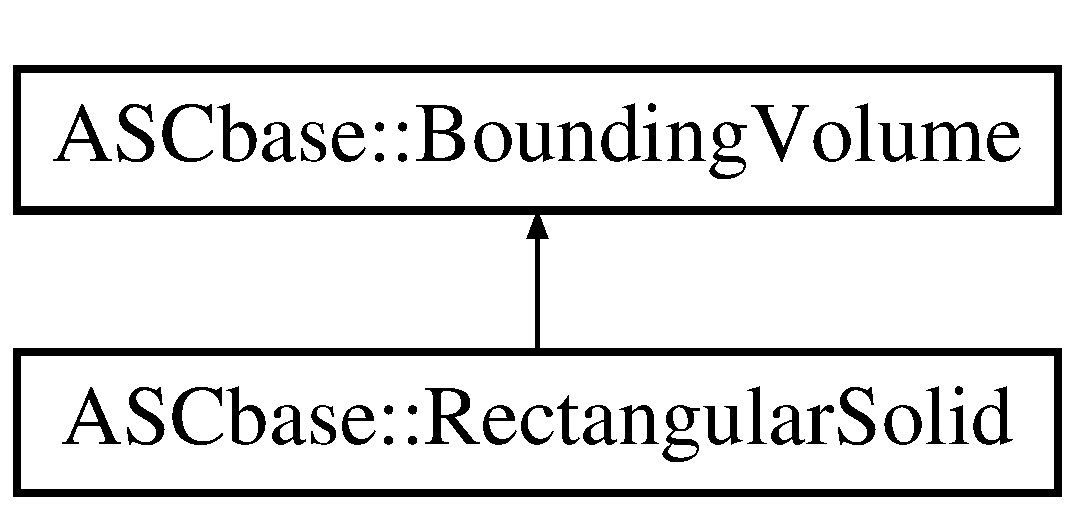
\includegraphics[height=2cm]{classASCbase_1_1RectangularSolid}
\end{center}
\end{figure}
\subsection*{Public Member Functions}
\begin{CompactItemize}
\item 
\textbf{Rectangular\-Solid} (const my\_\-float\_\-t $\ast$min\_\-corner\_\-in, const my\_\-float\_\-t $\ast$max\_\-corner\_\-in, const my\_\-float\_\-t grid\_\-spacing=0.0)\label{classASCbase_1_1RectangularSolid_6f27151311ea6c7c3036f033e55ce5bb}

\item 
\textbf{Rectangular\-Solid} (const \bf{Rectangular\-Solid} \&src)\label{classASCbase_1_1RectangularSolid_52a293bc179ad6858cf4c7f06937a224}

\item 
virtual bool \bf{contains} (const my\_\-float\_\-t $\ast$point) const \label{classASCbase_1_1RectangularSolid_a9e2c2a9ec3c034f3bba17219a7116c2}

\begin{CompactList}\small\item\em Is the given point inside the bounding volume? \item\end{CompactList}\item 
virtual bool \textbf{BIND\_\-vol\_\-contains} (const my\_\-float\_\-t $\ast$p) const \label{classASCbase_1_1RectangularSolid_3d17933ceada4081756d2e3f4a8bf6d2}

\item 
virtual bool \textbf{RAD\_\-vol\_\-contains} (const my\_\-float\_\-t $\ast$p) const \label{classASCbase_1_1RectangularSolid_888d6eb616e675241d0a3d11fb330a4f}

\item 
virtual size\_\-t \bf{discretize} (const my\_\-float\_\-t spacing, my\_\-float\_\-t $\ast$$\ast$grid\_\-pts)\label{classASCbase_1_1RectangularSolid_39443291990068ad369c9edfc75a4e76}

\begin{CompactList}\small\item\em discretize the volume using the spacing for grid spacing. \item\end{CompactList}\item 
virtual std::string \textbf{xml\_\-str} ()\label{classASCbase_1_1RectangularSolid_a8acf31a229ca25907a0d6cb85da4ec3}

\end{CompactItemize}
\subsection*{Private Attributes}
\begin{CompactItemize}
\item 
my\_\-float\_\-t \textbf{min\_\-corner} [3]\label{classASCbase_1_1RectangularSolid_a57a2744d2006581f35568bd2e43ea58}

\item 
my\_\-float\_\-t \textbf{max\_\-corner} [3]\label{classASCbase_1_1RectangularSolid_6d297afcc473c3cc2336c3017e7f638a}

\item 
my\_\-float\_\-t \textbf{BIND\_\-min\_\-corner} [3]\label{classASCbase_1_1RectangularSolid_fdbc647071b0beff1c695f5919eecf14}

\item 
my\_\-float\_\-t \textbf{BIND\_\-max\_\-corner} [3]\label{classASCbase_1_1RectangularSolid_bd9eb2d180cd46f6325a483d809c17f5}

\item 
my\_\-float\_\-t \textbf{RAD\_\-min\_\-corner} [3]\label{classASCbase_1_1RectangularSolid_f06af8b6554856ea2fb19d943c1a5b3b}

\item 
my\_\-float\_\-t \textbf{RAD\_\-max\_\-corner} [3]\label{classASCbase_1_1RectangularSolid_463d6a3ed40fa149db9cdccd456cd075}

\end{CompactItemize}


\subsection{Detailed Description}
A rectangular bounding volume. 



The documentation for this class was generated from the following files:\begin{CompactItemize}
\item 
Bounding\-Volume.H\item 
Bounding\-Volume.C\end{CompactItemize}

\section{ASCbase::residue\_\-conv\_\-type Struct Reference}
\label{structASCbase_1_1residue__conv__type}\index{ASCbase::residue_conv_type@{ASCbase::residue\_\-conv\_\-type}}
Silly little struct to help convert from string to residue name.  


{\tt \#include $<$PDB\_\-residues.H$>$}

\subsection*{Public Attributes}
\begin{CompactItemize}
\item 
residue\_\-type \textbf{residue}\label{structASCbase_1_1residue__conv__type_52f8acfdb1c1877592360527484b7da6}

\item 
std::string \textbf{name}\label{structASCbase_1_1residue__conv__type_a282bb2bec2f7ed9e2786ba3a5ac443b}

\end{CompactItemize}


\subsection{Detailed Description}
Silly little struct to help convert from string to residue name. 



The documentation for this struct was generated from the following file:\begin{CompactItemize}
\item 
PDB\_\-residues.H\end{CompactItemize}

\section{ASCbase::residue\_\-joints Class Reference}
\label{classASCbase_1_1residue__joints}\index{ASCbase::residue_joints@{ASCbase::residue\_\-joints}}
Data class to store the joints of one residue.  


{\tt \#include $<$prot\_\-joint\_\-dep.H$>$}

\subsection*{Public Member Functions}
\begin{CompactItemize}
\item 
\bf{residue\_\-joints} ()
\item 
\bf{residue\_\-joints} (const \bf{PDBStructure} $\ast$prot, residue\_\-vci res, const joint\_\-deps\_\-t \&res\_\-joints\_\-info)\label{classASCbase_1_1residue__joints_8c38f7e8122a28e0153347a1dfe1b30c}

\begin{CompactList}\small\item\em Default constructor for a given residue. \item\end{CompactList}\item 
\bf{residue\_\-joints} (const \bf{residue\_\-joints} \&other)\label{classASCbase_1_1residue__joints_f449cdad0ca876373713c618657b0015}

\begin{CompactList}\small\item\em Basic copy constructor. \item\end{CompactList}\item 
const \bf{residue\_\-joints} \& \bf{operator=} (const \bf{residue\_\-joints} \&other)\label{classASCbase_1_1residue__joints_a2cac3126dd4e9d9909fca1d3de2a53a}

\begin{CompactList}\small\item\em Basic assignment operator. \item\end{CompactList}\item 
\bf{$\sim$residue\_\-joints} ()\label{classASCbase_1_1residue__joints_d09831082869cc7230c1c6315615e33b}

\begin{CompactList}\small\item\em Basic destructor. \item\end{CompactList}\item 
void \bf{compute\_\-dihedral\_\-angles} (std::vector$<$ my\_\-float\_\-t $>$ $\ast$angles) const \label{classASCbase_1_1residue__joints_43413c481de3d0a00b610b8c445405cd}

\begin{CompactList}\small\item\em Compute the so called phi, psi, and chi angles of the residue. \item\end{CompactList}\item 
bool \bf{compute\_\-current\_\-axes\_\-of\_\-rotation} (my\_\-float\_\-t $\ast$rot\_\-axes, int $\ast$num\_\-axes, const int array\_\-len) const 
\item 
const int \textbf{num\_\-joints} () const \label{classASCbase_1_1residue__joints_6220137846303fb3cf73b4c02caaffd9}

\item 
const std::vector$<$ my\_\-float\_\-t $>$ \& \textbf{orig\_\-joint\_\-angles} () const \label{classASCbase_1_1residue__joints_45063f6a978d049bf4f5292b08241a93}

\item 
const bool \textbf{fail} ()\label{classASCbase_1_1residue__joints_fa5def7bc8d49c67da7ddc906f045c24}

\end{CompactItemize}
\subsection*{Public Attributes}
\begin{CompactItemize}
\item 
std::vector$<$ atom\_\-type $>$ \textbf{joint\_\-labels}\label{classASCbase_1_1residue__joints_61eee08b238efdfad0ec815eb47b0d26}

\item 
std::vector$<$ const my\_\-float\_\-t $\ast$ $>$ \bf{joint\_\-centers}\label{classASCbase_1_1residue__joints_a548886503607e03cdce112eb9ac92c9}

\begin{CompactList}\small\item\em Includes the CA position and one atom past the last joint. \item\end{CompactList}\end{CompactItemize}
\subsection*{Private Member Functions}
\begin{CompactItemize}
\item 
bool \textbf{check\_\-atom} (residue\_\-vci res, atom\_\-vci c\_\-atom, atom\_\-vci atoms\_\-end, atom\_\-type expected\_\-atom\_\-name)\label{classASCbase_1_1residue__joints_50f6fddea71680a7b814c8a1bf81e9c5}

\item 
void \textbf{do\_\-copy} (const \bf{residue\_\-joints} \&other)\label{classASCbase_1_1residue__joints_c48e538e71f2124731442e6d045710d5}

\item 
void \bf{init} ()\label{classASCbase_1_1residue__joints_8b3d0cf768de75423ff97aefdac11477}

\begin{CompactList}\small\item\em Initialize class variables. \item\end{CompactList}\item 
my\_\-float\_\-t \bf{compute\_\-dihedral\_\-angle} (const my\_\-float\_\-t $\ast$A, const my\_\-float\_\-t $\ast$B, const my\_\-float\_\-t $\ast$C) const 
\begin{CompactList}\small\item\em Compute the dihedral angle for the directional bond chain A, B, C. \item\end{CompactList}\item 
void \bf{warn\_\-cannot\_\-compute\_\-dihedral} (residue\_\-vci res, std::string angle\_\-name)\label{classASCbase_1_1residue__joints_49fe835a4836859911cf6ce15b275b51}

\begin{CompactList}\small\item\em A simple warning function to clean up the flow of the code. \item\end{CompactList}\end{CompactItemize}
\subsection*{Private Attributes}
\begin{CompactItemize}
\item 
residue\_\-type \textbf{A\_\-res\-Name}\label{classASCbase_1_1residue__joints_21497636be77aa78b659e24b4d60e350}

\item 
int \textbf{A\_\-num\_\-joints}\label{classASCbase_1_1residue__joints_bf4d7f0a200401c847a809f999ae2971}

\item 
bool \textbf{A\_\-fail}\label{classASCbase_1_1residue__joints_774042aeeddefb94221a85aef2a03eae}

\item 
const atom\_\-type $\ast$ \textbf{A\_\-atom\_\-names}\label{classASCbase_1_1residue__joints_5a33d4f7989653cd612fe8b6295e40a8}

\item 
const my\_\-float\_\-t $\ast$ \textbf{A\_\-atoms\_\-pos\_\-begin}\label{classASCbase_1_1residue__joints_36c3c3466b89a15fa509d32a83d97b9b}

\item 
const my\_\-float\_\-t $\ast$ \textbf{A\_\-atoms\_\-pos\_\-end}\label{classASCbase_1_1residue__joints_ae2d9bc7ca8ff776d6e1f46feb0c3f49}

\item 
const my\_\-float\_\-t $\ast$ \textbf{A\_\-prev\_\-res\_\-C\_\-pos}\label{classASCbase_1_1residue__joints_8fd8e62a05624a315c33809c1cf1bfb0}

\item 
const my\_\-float\_\-t $\ast$ \textbf{A\_\-next\_\-res\_\-N\_\-pos}\label{classASCbase_1_1residue__joints_c695ff8ec00bd34f913a43fe8087e7fa}

\item 
std::vector$<$ my\_\-float\_\-t $>$ \textbf{A\_\-orig\_\-joint\_\-angles}\label{classASCbase_1_1residue__joints_e0ccbfe40d2d00392c4d921188ad6361}

\end{CompactItemize}
\subsection*{Static Private Attributes}
\begin{CompactItemize}
\item 
static const std::string \textbf{A\_\-fname} = \char`\"{}prot\_\-joint\_\-dep\char`\"{}\label{classASCbase_1_1residue__joints_e39bf1e8f574aad44de1a4614d83a659}

\end{CompactItemize}


\subsection{Detailed Description}
Data class to store the joints of one residue. 



\subsection{Constructor \& Destructor Documentation}
\index{ASCbase::residue_joints@{ASCbase::residue\_\-joints}!residue_joints@{residue\_\-joints}}
\index{residue_joints@{residue\_\-joints}!ASCbase::residue_joints@{ASCbase::residue\_\-joints}}
\subsubsection{\setlength{\rightskip}{0pt plus 5cm}ASCbase::residue\_\-joints::residue\_\-joints ()\hspace{0.3cm}{\tt  [inline]}}\label{classASCbase_1_1residue__joints_1a5a5d456651261c8cfa2f1588f829de}


Default constructor -- used by maps, etc before applying the assignment operator 

\subsection{Member Function Documentation}
\index{ASCbase::residue_joints@{ASCbase::residue\_\-joints}!compute_current_axes_of_rotation@{compute\_\-current\_\-axes\_\-of\_\-rotation}}
\index{compute_current_axes_of_rotation@{compute\_\-current\_\-axes\_\-of\_\-rotation}!ASCbase::residue_joints@{ASCbase::residue\_\-joints}}
\subsubsection{\setlength{\rightskip}{0pt plus 5cm}bool residue\_\-joints::compute\_\-current\_\-axes\_\-of\_\-rotation (my\_\-float\_\-t $\ast$ {\em rot\_\-axes}, int $\ast$ {\em num\_\-axes}, const int {\em array\_\-len}) const}\label{classASCbase_1_1residue__joints_3a4671e36329ec606cfb9b1c91c7b334}


We need this function because we are relying on shallow copies (pointers rather) to atomic positions. Using this function makes it a bit less likely to have stale axes of rotation, rather than requiring explicit update of class variables after each moving of atoms (local and global). \index{ASCbase::residue_joints@{ASCbase::residue\_\-joints}!compute_dihedral_angle@{compute\_\-dihedral\_\-angle}}
\index{compute_dihedral_angle@{compute\_\-dihedral\_\-angle}!ASCbase::residue_joints@{ASCbase::residue\_\-joints}}
\subsubsection{\setlength{\rightskip}{0pt plus 5cm}my\_\-float\_\-t residue\_\-joints::compute\_\-dihedral\_\-angle (const my\_\-float\_\-t $\ast$ {\em A}, const my\_\-float\_\-t $\ast$ {\em B}, const my\_\-float\_\-t $\ast$ {\em C}) const\hspace{0.3cm}{\tt  [private]}}\label{classASCbase_1_1residue__joints_23107db1da4a4930345c2d1dacd44194}


Compute the dihedral angle for the directional bond chain A, B, C. 

\begin{Desc}
\item[Returns:]The dihedral angle in [-pi, pi] \end{Desc}


The documentation for this class was generated from the following files:\begin{CompactItemize}
\item 
prot\_\-joint\_\-dep.H\item 
prot\_\-joint\_\-dep.C\end{CompactItemize}

\section{ASCbase::residue\_\-t Class Reference}
\label{classASCbase_1_1residue__t}\index{ASCbase::residue_t@{ASCbase::residue\_\-t}}
Simple package to hold information about a PDB residue.  


{\tt \#include $<$PDBStructure.H$>$}

\subsection*{Public Member Functions}
\begin{CompactItemize}
\item 
\bf{residue\_\-t} (atom\_\-vci atom)\label{classASCbase_1_1residue__t_673a2f705f7d90b695899287ca440a17}

\begin{CompactList}\small\item\em Initialize residue based on the given atom. \item\end{CompactList}\item 
atom\_\-vci \textbf{get\_\-atom} (atom\_\-type atom\_\-name) const \label{classASCbase_1_1residue__t_2e728f3de20c3259a7b63843a8de7932}

\end{CompactItemize}
\subsection*{Public Attributes}
\begin{CompactItemize}
\item 
residue\_\-type \bf{name}\label{classASCbase_1_1residue__t_d33ebf59abe10245839a2e3e976f28b6}

\begin{CompactList}\small\item\em 3 character name of the residue \item\end{CompactList}\item 
uint \bf{number}\label{classASCbase_1_1residue__t_f22f101c1c4287d1f7217e8a4a3ef882}

\begin{CompactList}\small\item\em Number assigned to residue in the PDB file. \item\end{CompactList}\item 
char \bf{icode}\label{classASCbase_1_1residue__t_9ba317e5ba32fc025f3405bce5bcfc3d}

\begin{CompactList}\small\item\em Insertion code assigned to the residue. \item\end{CompactList}\item 
char \bf{chain\-ID}\label{classASCbase_1_1residue__t_a22d41efc884bf49196aedf45456668d}

\begin{CompactList}\small\item\em Chain ID assigned to the residue. \item\end{CompactList}\item 
atom\_\-vci \bf{atoms\_\-begin}\label{classASCbase_1_1residue__t_a0aecc888b54e490610196493aae54c9}

\begin{CompactList}\small\item\em Iterator to first atom in the residue. \item\end{CompactList}\item 
atom\_\-vci \bf{atoms\_\-end}\label{classASCbase_1_1residue__t_9315cf7728dc09465af606000f04bcf7}

\begin{CompactList}\small\item\em Iterator to 1 past the last atom in the residue. \item\end{CompactList}\item 
bool \bf{is\_\-MODRES}\label{classASCbase_1_1residue__t_d37b0dfb9a32c77e2ae2c167008d39a3}

\begin{CompactList}\small\item\em True implies this residue corresponds to a MODRES. \item\end{CompactList}\item 
bool \bf{is\_\-HET}\label{classASCbase_1_1residue__t_78e29c2b3e395dae09614d59d45309d4}

\begin{CompactList}\small\item\em True implies this residue corresponds to a HET record. \item\end{CompactList}\end{CompactItemize}


\subsection{Detailed Description}
Simple package to hold information about a PDB residue. 



The documentation for this class was generated from the following file:\begin{CompactItemize}
\item 
PDBStructure.H\end{CompactItemize}

\section{ASCbase::rigid\_\-align\_\-t Class Reference}
\label{classASCbase_1_1rigid__align__t}\index{ASCbase::rigid_align_t@{ASCbase::rigid\_\-align\_\-t}}
Data class: Holds the numerous features of an alignment.  


{\tt \#include $<$Score\-Map\-Base.H$>$}

Inheritance diagram for ASCbase::rigid\_\-align\_\-t::\begin{figure}[H]
\begin{center}
\leavevmode
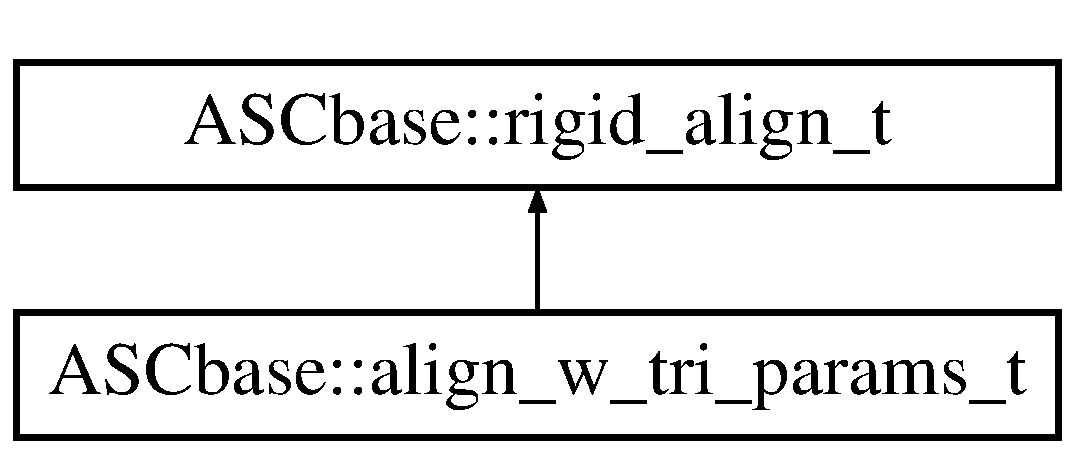
\includegraphics[height=2cm]{classASCbase_1_1rigid__align__t}
\end{center}
\end{figure}
\subsection*{Public Member Functions}
\begin{CompactItemize}
\item 
\bf{rigid\_\-align\_\-t} ()\label{classASCbase_1_1rigid__align__t_e6335cc41892b44aba75afb30c42422b}

\begin{CompactList}\small\item\em Initialize the features to zero or very large values. \item\end{CompactList}\item 
\bf{rigid\_\-align\_\-t} (const \bf{rigid\_\-align\_\-t} \&other)\label{classASCbase_1_1rigid__align__t_e05610ac44e3120513667837de227445}

\begin{CompactList}\small\item\em Basic copy constructor. \item\end{CompactList}\item 
const \bf{rigid\_\-align\_\-t} \& \bf{operator=} (const \bf{rigid\_\-align\_\-t} \&other)\label{classASCbase_1_1rigid__align__t_e42d7414871c06710daf9f23d71d349d}

\begin{CompactList}\small\item\em Basic assignment operator. \item\end{CompactList}\item 
virtual \bf{$\sim$rigid\_\-align\_\-t} ()\label{classASCbase_1_1rigid__align__t_be237ac53c1d6917a5ff2c717574b955}

\begin{CompactList}\small\item\em Do nothing destructor. \item\end{CompactList}\item 
bool \bf{operator==} (const \bf{rigid\_\-align\_\-t} \&b) const 
\item 
bool \bf{operator!=} (const \bf{rigid\_\-align\_\-t} \&b) const 
\item 
virtual void \textbf{write\_\-score\_\-fields} (std::ostream \&out, const uint orient\_\-num, const bool wrote\_\-ligs, const std::string \&ext\_\-SF\_\-id\_\-in, const std::string \&struct\_\-id, const std::string \&lig\_\-id) const \label{classASCbase_1_1rigid__align__t_12c292600e42cb9e61a87201d38b574d}

\item 
virtual void \textbf{write\_\-score\_\-fields} (std::ostream \&out) const \label{classASCbase_1_1rigid__align__t_c02636bc474643f5ceb468212ce470db}

\item 
virtual void \textbf{get\_\-score\_\-field\_\-labels} (std::vector$<$ std::string $>$ $\ast$fields, const bool normalize\_\-score) const \label{classASCbase_1_1rigid__align__t_c276978bf665b4f8899893f929333acf}

\item 
virtual void \textbf{set\_\-prot\_\-lig\_\-scores} (const my\_\-float\_\-t affiscore, const my\_\-float\_\-t orientscore, const my\_\-float\_\-t ligand\_\-efficiency)\label{classASCbase_1_1rigid__align__t_ab98b09f549c3700c63a772e495c8858}

\item 
virtual void \textbf{set\_\-triangle\_\-params} (const my\_\-float\_\-t perimeter, const my\_\-float\_\-t long\_\-len, const my\_\-float\_\-t short\_\-len)\label{classASCbase_1_1rigid__align__t_46db34052a8e92e8b9455b4d3adc4fa4}

\item 
virtual void \textbf{set\_\-number\_\-of\_\-orientations} (const size\_\-t num)\label{classASCbase_1_1rigid__align__t_482bac50e100ac69fb62edd5b3ff6775}

\item 
virtual void \textbf{save\_\-rigid\_\-alignment\_\-vals} ()\label{classASCbase_1_1rigid__align__t_b05738bb2695109d10c7b553ac7b4e42}

\item 
virtual void \textbf{save\_\-pre\-IK\_\-vals} ()\label{classASCbase_1_1rigid__align__t_8d323747e24f9374c1a94b364c3c415d}

\item 
virtual bool \textbf{compute\_\-prot\_\-lig\_\-score} ()\label{classASCbase_1_1rigid__align__t_b14c62f28834c0c953753b108954052e}

\item 
virtual void \textbf{set\_\-site\_\-atomic\_\-rmsd} (const my\_\-float\_\-t rmsd, const size\_\-t rmsd\_\-type)\label{classASCbase_1_1rigid__align__t_7f27991120704fa2a19cb8a7cf31ce55}

\end{CompactItemize}
\subsection*{Public Attributes}
\begin{CompactItemize}
\item 
my\_\-float\_\-t \bf{tier1\_\-score}\label{classASCbase_1_1rigid__align__t_1fef21d1eb205408a96f533891e79557}

\begin{CompactList}\small\item\em ASCbase fast orientation score (sieve). \item\end{CompactList}\item 
my\_\-float\_\-t \bf{score}\label{classASCbase_1_1rigid__align__t_90a54e487c78c50e21dcb7f781cc37ef}

\begin{CompactList}\small\item\em Final ASCbase score -- tier2. \item\end{CompactList}\item 
std::vector$<$ my\_\-float\_\-t $>$ \textbf{terms}\label{classASCbase_1_1rigid__align__t_6cf98bc92eac939ebe592ae47a49446a}

\item 
std::vector$<$ my\_\-float\_\-t $>$ \bf{ext\_\-scores}\label{classASCbase_1_1rigid__align__t_0ce6360ea3d61818cd088f34f2cf118d}

\begin{CompactList}\small\item\em External score(s). \item\end{CompactList}\item 
std::vector$<$ bool $>$ \textbf{frag\_\-atoms\_\-flags}\label{classASCbase_1_1rigid__align__t_8a3efbcef870f53faa51a54e64918e17}

\item 
my\_\-float\_\-t \bf{R} [9]\label{classASCbase_1_1rigid__align__t_c19150913ee8369262f89abf3dba1839}

\begin{CompactList}\small\item\em Rotation matrix for search to query. \item\end{CompactList}\item 
my\_\-float\_\-t \bf{T} [3]\label{classASCbase_1_1rigid__align__t_c66d5098258a0e0296c47b3d438dfd40}

\begin{CompactList}\small\item\em Translation vector for search to query. \item\end{CompactList}\item 
Quaternion \textbf{Q}\label{classASCbase_1_1rigid__align__t_ffd3c5b8182230bf24cc1ae954039360}

\item 
\bf{mol2File} $\ast$ \bf{frag\_\-file}\label{classASCbase_1_1rigid__align__t_be34b21f5d3ef687d3e9213aca149eb6}

\begin{CompactList}\small\item\em Pointer to the ligand fragment in query pocket. \item\end{CompactList}\item 
std::vector$<$ bool $>$ \textbf{match\_\-print}\label{classASCbase_1_1rigid__align__t_21450c7e527409561c1eaee7f46bf922}

\item 
my\_\-float\_\-t \textbf{hb\_\-caps\_\-score}\label{classASCbase_1_1rigid__align__t_956a632cdccaa9096759d9c1d38c6026}

\item 
std::string \textbf{hb\_\-caps\_\-match\_\-print}\label{classASCbase_1_1rigid__align__t_bd736c82ab7b0c5704c58fd85ca836a1}

\end{CompactItemize}
\subsection*{Private Member Functions}
\begin{CompactItemize}
\item 
void \textbf{init} ()\label{classASCbase_1_1rigid__align__t_19b9ab1fc878784b26ed6bf7a5d2338f}

\item 
void \bf{do\_\-copy} (const \bf{rigid\_\-align\_\-t} \&other)\label{classASCbase_1_1rigid__align__t_ab8efcf8e3820a7e91cd135acef58c84}

\begin{CompactList}\small\item\em A straightforward copy method. \item\end{CompactList}\end{CompactItemize}


\subsection{Detailed Description}
Data class: Holds the numerous features of an alignment. 

This class was supposed to make it easier to swap things in and out. However, it was put together relatively quickly and its major design flaw is that one cannot pick and choose score fields. It might be useful for future development if one can pick and choose pieces for scoring and reporting. 



\subsection{Member Function Documentation}
\index{ASCbase::rigid_align_t@{ASCbase::rigid\_\-align\_\-t}!operator"!=@{operator"!=}}
\index{operator"!=@{operator"!=}!ASCbase::rigid_align_t@{ASCbase::rigid\_\-align\_\-t}}
\subsubsection{\setlength{\rightskip}{0pt plus 5cm}bool ASCbase::rigid\_\-align\_\-t::operator!= (const \bf{rigid\_\-align\_\-t} \& {\em b}) const\hspace{0.3cm}{\tt  [inline]}}\label{classASCbase_1_1rigid__align__t_dd0fdb2785fd9d00e710d9afd3253f4a}


Two alignments are not equal if their score is not the same or they do not have the same transformation \index{ASCbase::rigid_align_t@{ASCbase::rigid\_\-align\_\-t}!operator==@{operator==}}
\index{operator==@{operator==}!ASCbase::rigid_align_t@{ASCbase::rigid\_\-align\_\-t}}
\subsubsection{\setlength{\rightskip}{0pt plus 5cm}bool ASCbase::rigid\_\-align\_\-t::operator== (const \bf{rigid\_\-align\_\-t} \& {\em b}) const\hspace{0.3cm}{\tt  [inline]}}\label{classASCbase_1_1rigid__align__t_3f01290c1017cdf9f9e1e6a3bf7af5ac}


Two alignments are equal if their score is the same and they have the same transformation 

The documentation for this class was generated from the following files:\begin{CompactItemize}
\item 
Score\-Map\-Base.H\item 
Score\-Map\-Base.C\end{CompactItemize}

\section{ASCbase::Score\-Map\-Base Class Reference}
\label{classASCbase_1_1ScoreMapBase}\index{ASCbase::ScoreMapBase@{ASCbase::ScoreMapBase}}
{\tt \#include $<$Score\-Map\-Base.H$>$}

Inheritance diagram for ASCbase::Score\-Map\-Base::\begin{figure}[H]
\begin{center}
\leavevmode
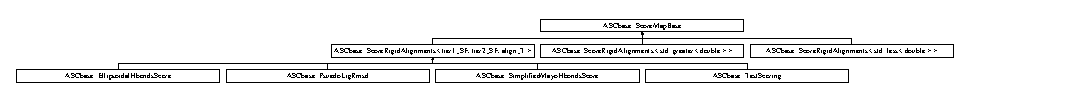
\includegraphics[height=0.88189cm]{classASCbase_1_1ScoreMapBase}
\end{center}
\end{figure}
\subsection*{Public Member Functions}
\begin{CompactItemize}
\item 
\bf{Score\-Map\-Base} (const \bf{Search\-Parameters} \&params)
\item 
virtual \bf{$\sim$Score\-Map\-Base} ()\label{classASCbase_1_1ScoreMapBase_53cc54d782902810408e5e4ebcbbffd5}

\begin{CompactList}\small\item\em basic destruction \item\end{CompactList}\item 
bool \bf{set\_\-external\_\-scoring\_\-method} (const std::string sf\_\-name, std::string method\_\-name)
\item 
template$<$class align\_\-mmap\_\-iter$>$ bool \bf{run\_\-external\_\-scoring\_\-method} (align\_\-mmap\_\-iter a\_\-beg, align\_\-mmap\_\-iter a\_\-end, const std::string \&prot\_\-fname, const std::string \&struct\_\-id, const std::string \&output\_\-dir)
\begin{CompactList}\small\item\em Run the external scoring function over all the saved alignments. \item\end{CompactList}\item 
void \bf{get\_\-ext\_\-SF\_\-names} (std::vector$<$ std::string $>$ $\ast$names)\label{classASCbase_1_1ScoreMapBase_b5ee9de7e756e9c6ee3058c475a95958}

\begin{CompactList}\small\item\em Get the name(s) of the external scoring function(s). \item\end{CompactList}\end{CompactItemize}
\subsection*{Protected Attributes}
\begin{CompactItemize}
\item 
std::string \textbf{A\_\-scratch\_\-dir}\label{classASCbase_1_1ScoreMapBase_784728589fd2db54ce16e5043db3c349}

\item 
bool \bf{A\_\-write\_\-ligands}\label{classASCbase_1_1ScoreMapBase_c11f067cce7e9e72f38b4cdc2abde485}

\begin{CompactList}\small\item\em True =$>$ write ligs and frags, else do not write. \item\end{CompactList}\item 
bool \bf{A\_\-prot\_\-lig\_\-score}\label{classASCbase_1_1ScoreMapBase_42d2d13e5fa5d7492495dd531246f8a5}

\begin{CompactList}\small\item\em True ==$>$ compute query prot -- dbase lig frag affi and orient scores. \item\end{CompactList}\item 
std::string \bf{ext\_\-SF\_\-id}\label{classASCbase_1_1ScoreMapBase_b6bfd4fcc3263c7ee1cc86c856cea184}

\begin{CompactList}\small\item\em Label given to the ext. prot-lig scoring fcn. \item\end{CompactList}\end{CompactItemize}
\subsection*{Private Attributes}
\begin{CompactItemize}
\item 
\bf{External\-Scoring\-Function} $\ast$ \bf{A\_\-external\_\-SF}\label{classASCbase_1_1ScoreMapBase_490667b180269340cbf0017b282eabb6}

\begin{CompactList}\small\item\em external prot-lig score fcn ptr \item\end{CompactList}\end{CompactItemize}


\subsection{Detailed Description}
Because of the gcc model, we must have all template definitions included in all the source files which use the functions, classes, etc that are prototyped and defined using the template keyword. 



\subsection{Constructor \& Destructor Documentation}
\index{ASCbase::ScoreMapBase@{ASCbase::Score\-Map\-Base}!ScoreMapBase@{ScoreMapBase}}
\index{ScoreMapBase@{ScoreMapBase}!ASCbase::ScoreMapBase@{ASCbase::Score\-Map\-Base}}
\subsubsection{\setlength{\rightskip}{0pt plus 5cm}ASCbase::Score\-Map\-Base::Score\-Map\-Base (const \bf{Search\-Parameters} \& {\em params})\hspace{0.3cm}{\tt  [inline]}}\label{classASCbase_1_1ScoreMapBase_17c627b5ef8a777466b2f9ebc50bd228}


\begin{Desc}
\item[Parameters:]
\begin{description}
\item[{\em params}]Reference to the search's runtime parameters \end{description}
\end{Desc}


\subsection{Member Function Documentation}
\index{ASCbase::ScoreMapBase@{ASCbase::Score\-Map\-Base}!run_external_scoring_method@{run\_\-external\_\-scoring\_\-method}}
\index{run_external_scoring_method@{run\_\-external\_\-scoring\_\-method}!ASCbase::ScoreMapBase@{ASCbase::Score\-Map\-Base}}
\subsubsection{\setlength{\rightskip}{0pt plus 5cm}template$<$class align\_\-mmap\_\-iter$>$ bool ASCbase::Score\-Map\-Base::run\_\-external\_\-scoring\_\-method (align\_\-mmap\_\-iter {\em a\_\-beg}, align\_\-mmap\_\-iter {\em a\_\-end}, const std::string \& {\em prot\_\-fname}, const std::string \& {\em struct\_\-id}, const std::string \& {\em output\_\-dir})\hspace{0.3cm}{\tt  [inline]}}\label{classASCbase_1_1ScoreMapBase_85708eaffffc9a4e36bbd7375b552586}


Run the external scoring function over all the saved alignments. 

For a given ASCbase run, the model sitemap is held constant. Thus, we need only one protein\_\-file. For each saved alignment, score the protein and the saved ligand fragment.

\begin{Desc}
\item[Parameters:]
\begin{description}
\item[{\em protein\_\-file}]Protein PDB corresponding to the model sitemap \item[{\em output\_\-dir}]Directory holding the ligand fragments \end{description}
\end{Desc}
\begin{Desc}
\item[Returns:]True if the scoring function was initialized, else false \end{Desc}
\index{ASCbase::ScoreMapBase@{ASCbase::Score\-Map\-Base}!set_external_scoring_method@{set\_\-external\_\-scoring\_\-method}}
\index{set_external_scoring_method@{set\_\-external\_\-scoring\_\-method}!ASCbase::ScoreMapBase@{ASCbase::Score\-Map\-Base}}
\subsubsection{\setlength{\rightskip}{0pt plus 5cm}bool ASCbase::Score\-Map\-Base::set\_\-external\_\-scoring\_\-method (const std::string {\em sf\_\-name}, std::string {\em method\_\-name})\hspace{0.3cm}{\tt  [inline]}}\label{classASCbase_1_1ScoreMapBase_d24ec72fca67bdacb134c71a0e78e9d6}


Setup the external scoring function. This function is in this class since it acts as a storage class for the alignments

\begin{Desc}
\item[Parameters:]
\begin{description}
\item[{\em sf\_\-name}]Path to the external scoring function file \item[{\em method\_\-name}]Name of the external scoring function (as stored in the external\_\-scoring\_\-functions.txt file) \end{description}
\end{Desc}
\begin{Desc}
\item[Returns:]True if method was found, else false \end{Desc}


The documentation for this class was generated from the following file:\begin{CompactItemize}
\item 
Score\-Map\-Base.H\end{CompactItemize}

\section{ASCbase::Score\-Rigid\-Alignments$<$ tier1\_\-SF, tier2\_\-SF, align\_\-T $>$ Class Template Reference}
\label{classASCbase_1_1ScoreRigidAlignments}\index{ASCbase::ScoreRigidAlignments@{ASCbase::ScoreRigidAlignments}}
{\tt \#include $<$Score\-Rigid\-Alignments.H$>$}

Inheritance diagram for ASCbase::Score\-Rigid\-Alignments$<$ tier1\_\-SF, tier2\_\-SF, align\_\-T $>$::\begin{figure}[H]
\begin{center}
\leavevmode
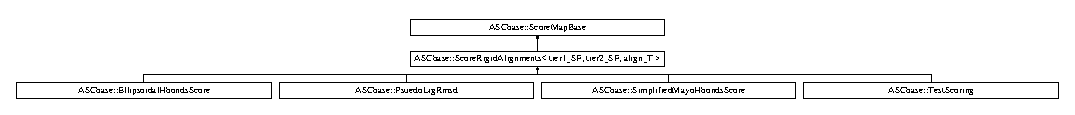
\includegraphics[height=1.10236cm]{classASCbase_1_1ScoreRigidAlignments}
\end{center}
\end{figure}
\subsection*{Public Types}
\begin{CompactItemize}
\item 
typedef align\_\-T \textbf{rigid\_\-align\_\-obj}\label{classASCbase_1_1ScoreRigidAlignments_b70f013e31f873b416a5c56f027bf72b}

\item 
typedef std::vector$<$ align\_\-T $>$ \textbf{rigid\_\-align\_\-vec}\label{classASCbase_1_1ScoreRigidAlignments_b3f6b33427a5b3e1b3dc7f0f08f7c938}

\item 
typedef rigid\_\-align\_\-vec::iterator \textbf{rigid\_\-align\_\-vi}\label{classASCbase_1_1ScoreRigidAlignments_9197e08d6673598fff132c83c333ad16}

\item 
typedef rigid\_\-align\_\-vec::const\_\-iterator \textbf{rigid\_\-align\_\-vci}\label{classASCbase_1_1ScoreRigidAlignments_fd3610658be7ab3a2f7a878c765be502}

\item 
typedef std::pair$<$ my\_\-float\_\-t, rigid\_\-align\_\-vi $>$ \textbf{align\_\-pair}\label{classASCbase_1_1ScoreRigidAlignments_098b2ec3327dc70824a300518f04b533}

\item 
typedef tier1\_\-SF::score\_\-cmp \textbf{tier1\_\-score\_\-cmp}\label{classASCbase_1_1ScoreRigidAlignments_2e5d9eff65db2ea8f48b1b559cff47ec}

\item 
typedef tier2\_\-SF::score\_\-cmp \textbf{tier2\_\-score\_\-cmp}\label{classASCbase_1_1ScoreRigidAlignments_4da6a8b332409ba4f92872b12d29f907}

\item 
typedef std::multimap$<$ my\_\-float\_\-t, rigid\_\-align\_\-vi, tier1\_\-score\_\-cmp $>$ \textbf{tier1\_\-score\_\-mmap}\label{classASCbase_1_1ScoreRigidAlignments_8f27b9efe358dc67f0f93da09994267c}

\item 
typedef std::multimap$<$ my\_\-float\_\-t, rigid\_\-align\_\-vi, tier2\_\-score\_\-cmp $>$ \textbf{tier2\_\-score\_\-mmap}\label{classASCbase_1_1ScoreRigidAlignments_c12679175ba1bf637a930445a2c5ecf9}

\item 
typedef tier1\_\-score\_\-mmap::iterator \textbf{tier1\_\-score\_\-mmi}\label{classASCbase_1_1ScoreRigidAlignments_c7e09e3ab6898aa2255a87ee3f46c8cd}

\item 
typedef tier2\_\-score\_\-mmap::iterator \textbf{tier2\_\-score\_\-mmi}\label{classASCbase_1_1ScoreRigidAlignments_dd2d97ba42597faa5ad8a422bc074154}

\item 
typedef tier1\_\-score\_\-mmap::const\_\-iterator \textbf{tier1\_\-score\_\-mmci}\label{classASCbase_1_1ScoreRigidAlignments_a47352558a34670ebbcd3351717d544f}

\item 
typedef tier2\_\-score\_\-mmap::const\_\-iterator \textbf{tier2\_\-score\_\-mmci}\label{classASCbase_1_1ScoreRigidAlignments_c4678b6b9b54e64357d663f1dd69bd36}

\end{CompactItemize}
\subsection*{Public Member Functions}
\begin{CompactItemize}
\item 
\bf{Score\-Rigid\-Alignments} (\bf{Model\-Sitemap} $\ast$model\_\-in, const \bf{Search\-Parameters} \&params)
\begin{CompactList}\small\item\em Default constructor for scoring methods of rigidly aligned sitemaps. \item\end{CompactList}\item 
\bf{$\sim$Score\-Rigid\-Alignments} ()\label{classASCbase_1_1ScoreRigidAlignments_9c5edad1dcd9af6c0150ef7d8429ad47}

\begin{CompactList}\small\item\em basic destruction \item\end{CompactList}\item 
bool \bf{score\_\-alignments} (rigid\_\-align\_\-vec \&aligns, \bf{Dbase\-Sitemap} $\ast$dbase\_\-site, std::ostream \&results\_\-out=std::cout, std::ostream \&rigid\_\-results\_\-out=std::cout)
\begin{CompactList}\small\item\em Main scoring routine. \item\end{CompactList}\item 
virtual void \bf{write\_\-score\_\-header} (std::ostream \&out)\label{classASCbase_1_1ScoreRigidAlignments_3668ef98e3e48111f868cfd5ee139565}

\begin{CompactList}\small\item\em Needs to be called before scoring any alignments. \item\end{CompactList}\item 
bool \bf{score\_\-tier1\_\-alignments} (rigid\_\-align\_\-vec \&aligns\_\-in, \bf{Dbase\-Sitemap} $\ast$search, \bf{mol2File} $\ast$lig\_\-file, tier1\_\-score\_\-mmap $\ast$top\_\-aligns)
\begin{CompactList}\small\item\em Score the alignments for 1 model, search pair of sitemaps. \item\end{CompactList}\item 
bool \bf{score\_\-tier2\_\-alignments} (tier1\_\-score\_\-mmap \&align\_\-map, \bf{Dbase\-Sitemap} $\ast$dset\_\-site, \bf{mol2File} $\ast$lig\_\-file, const std::string \&db\_\-struct\_\-id, const std::string \&db\_\-mol\_\-id, tier2\_\-score\_\-mmap $\ast$top\_\-aligns, std::ostream \&rigid\_\-results\_\-out)\label{classASCbase_1_1ScoreRigidAlignments_280977dd9ab68c9c274ede4ad3bf8c1c}

\begin{CompactList}\small\item\em Score the alignments that passed the first sieve. \item\end{CompactList}\item 
bool \bf{score\_\-alignments} (rigid\_\-align\_\-vec \&aligns\_\-in, \bf{Dbase\-Sitemap} $\ast$dset\_\-site, \bf{mol2File} $\ast$lig\_\-file, const std::string \&db\_\-struct\_\-id, const std::string \&db\_\-mol\_\-id, tier2\_\-score\_\-mmap $\ast$top\_\-aligns, std::ostream \&rigid\_\-results\_\-out)
\begin{CompactList}\small\item\em Score the alignments for 1 model, dset pair of sitemaps. \item\end{CompactList}\item 
template$<$class score\_\-T, class cmp\_\-T$>$ bool \textbf{blah} (rigid\_\-align\_\-vi align, score\_\-T $\ast$score\_\-method, cmp\_\-T score\_\-cmp, std::multimap$<$ my\_\-float\_\-t, rigid\_\-align\_\-vi, cmp\_\-T $>$ $\ast$top\_\-aligns, \bf{mol2File} $\ast$lig\_\-file, const bool frag\_\-lig\_\-filter, const size\_\-t max\_\-num\_\-aligns, const my\_\-float\_\-t score\_\-cutoff, const bool fine\_\-tune\_\-all, \bf{Dbase\-Sitemap} $\ast$dset\_\-site)\label{classASCbase_1_1ScoreRigidAlignments_f4161aac72991c94e45dcd6b9d6629ff}

\item 
template$<$class score\_\-T$>$ void \bf{refine\_\-best\_\-alignment} (score\_\-T $\ast$score\_\-method, tier2\_\-score\_\-mmap $\ast$top\_\-aligns, \bf{Dbase\-Sitemap} $\ast$dset\_\-site, \bf{mol2File} $\ast$lig\_\-file, const std::string \&db\_\-struct\_\-id, const std::string \&db\_\-mol\_\-id, std::ostream \&rigid\_\-results\_\-out)
\item 
void \bf{score\_\-protein\_\-ligand\_\-interactions} (tier2\_\-score\_\-mmap $\ast$top\_\-aligns)\label{classASCbase_1_1ScoreRigidAlignments_4e0ef1c8fe1ed27a93385ec78ca35bf7}

\begin{CompactList}\small\item\em Score protein-ligand interactions for the saved alignments. \item\end{CompactList}\item 
void \bf{handle\_\-ligands} (tier2\_\-score\_\-mmap \&top\_\-aligns, \bf{mol2File} $\ast$lig\_\-file, const std::string \&mol\_\-id)\label{classASCbase_1_1ScoreRigidAlignments_4adb8e45da74e0d142fd29e1b1f104dc}

\begin{CompactList}\small\item\em Handle the ligands for the saved alignments. \item\end{CompactList}\item 
void \bf{report\_\-alignments} (const tier2\_\-score\_\-mmap top\_\-aligns, const bool wrote\_\-ligs, const std::string \&db\_\-struct\_\-id, const std::string \&db\_\-mol\_\-id, std::ostream \&results\_\-out)\label{classASCbase_1_1ScoreRigidAlignments_ec86b7fcea8af70b5b4e7cb7dc87383a}

\begin{CompactList}\small\item\em Loop to print out the saved alignments. \item\end{CompactList}\item 
virtual void \bf{fine\_\-tune\_\-align} (\bf{Dbase\-Sitemap} $\ast$search, rigid\_\-align\_\-obj $\ast$align)
\item 
const std::string \& \textbf{model\_\-struct\_\-id} ()\label{classASCbase_1_1ScoreRigidAlignments_206d3c0c67dd76415e95d0272c254dc3}

\end{CompactItemize}
\subsection*{Public Attributes}
\begin{CompactItemize}
\item 
tier1\_\-SF \textbf{A\_\-tier1\_\-score\_\-class}\label{classASCbase_1_1ScoreRigidAlignments_b63c437199f354cf7e9ed6d8ffc19016}

\item 
tier2\_\-SF \textbf{A\_\-tier2\_\-score\_\-class}\label{classASCbase_1_1ScoreRigidAlignments_32969be6699fb353d5952e05f63ff87c}

\end{CompactItemize}
\subsection*{Protected Member Functions}
\begin{CompactItemize}
\item 
bool \bf{load\_\-ligand} (const std::string \&lig\_\-fname, const std::string \&atoms\_\-fname, \bf{mol2File} $\ast$$\ast$ligand, std::string $\ast$struct\_\-id, std::string $\ast$mol\_\-id)\label{classASCbase_1_1ScoreRigidAlignments_a2c37b383be18dec552610eacad948fa}

\begin{CompactList}\small\item\em Load the database ligand file. \item\end{CompactList}\item 
bool \textbf{get\_\-ligand\_\-fragment} (const \bf{mol2File} \&lig\_\-file, const \bf{Bounding\-Volume} \&site\_\-vol, const \bf{Coord\-File} \&interacting\_\-atoms, \bf{rigid\_\-align\_\-t} $\ast$align)\label{classASCbase_1_1ScoreRigidAlignments_c83e7a7d636e879db4e6f4c135a4a9af}

\item 
\bf{Model\-Sitemap} $\ast$ \textbf{model} ()\label{classASCbase_1_1ScoreRigidAlignments_eb21d7327bbf06dcc3d4debab2c37be8}

\item 
const my\_\-float\_\-t \textbf{mu} () const \label{classASCbase_1_1ScoreRigidAlignments_876a98ad43a52edf8cc3ffcbc430c5d1}

\item 
const my\_\-float\_\-t \textbf{sigma} () const \label{classASCbase_1_1ScoreRigidAlignments_22d5f99e1d0b51848ba4f7398cf65ebf}

\item 
const bool \textbf{fine\_\-tune\_\-tier2\_\-alignments} () const \label{classASCbase_1_1ScoreRigidAlignments_92597bda9278cb646d53f52607f11fe3}

\item 
\bf{IK\_\-tests} \& \textbf{IK\_\-tests\_\-handle} ()\label{classASCbase_1_1ScoreRigidAlignments_df0cb37b9cd68a3ba04aa250fd343a32}

\item 
const bool \textbf{do\_\-IK} () const \label{classASCbase_1_1ScoreRigidAlignments_f59c733a2e67e63da9ae49477949ced2}

\end{CompactItemize}
\subsection*{Protected Attributes}
\begin{CompactItemize}
\item 
tier1\_\-score\_\-cmp \bf{A\_\-tier1\_\-score\_\-cmp}\label{classASCbase_1_1ScoreRigidAlignments_13a5468270fa523e191d1428030fd015}

\begin{CompactList}\small\item\em Get an instance of tier1 cmp. \item\end{CompactList}\item 
tier2\_\-score\_\-cmp \bf{A\_\-tier2\_\-score\_\-cmp}\label{classASCbase_1_1ScoreRigidAlignments_f70ab6bb6b22b59758853f0326c8fece}

\begin{CompactList}\small\item\em Get an instance of tier2 cmp. \item\end{CompactList}\end{CompactItemize}
\subsection*{Private Member Functions}
\begin{CompactItemize}
\item 
void \bf{write\_\-ligands} (\bf{mol2File} $\ast$frag\_\-file, \bf{mol2File} $\ast$lig\_\-file, const my\_\-float\_\-t $\ast$R, const my\_\-float\_\-t $\ast$T, const uint cnt, const std::string struct\_\-id, const std::string output\_\-dir)
\begin{CompactList}\small\item\em Write out the saved ligands and ligand fragments. \item\end{CompactList}\end{CompactItemize}
\subsection*{Private Attributes}
\begin{CompactItemize}
\item 
\bf{Model\-Sitemap} $\ast$ \bf{A\_\-model}\label{classASCbase_1_1ScoreRigidAlignments_74c601b35ff79d35a71f0fc155aeaab0}

\begin{CompactList}\small\item\em The model sitemap -- this is not a constant pointer since we may desire to transform the model rather than dbase site. \item\end{CompactList}\item 
std::string \textbf{A\_\-score\_\-method\_\-str}\label{classASCbase_1_1ScoreRigidAlignments_78b29cd62788f0e58a57f1e545b6ca78}

\item 
\bf{IK\_\-tests} \textbf{A\_\-my\_\-IK}\label{classASCbase_1_1ScoreRigidAlignments_aea65d1bae615f534f6f8543746e423c}

\item 
bool \textbf{A\_\-struct\_\-id\_\-field}\label{classASCbase_1_1ScoreRigidAlignments_6b70faffcbc103668446433a12d6dd89}

\item 
std::string \textbf{A\_\-model\_\-struct\_\-id}\label{classASCbase_1_1ScoreRigidAlignments_6107f30f22441300a2d9511fbe0eebb0}

\item 
my\_\-float\_\-t \bf{A\_\-mu}\label{classASCbase_1_1ScoreRigidAlignments_e2a77ac5a0d9b23d4149c04dde1e445d}

\begin{CompactList}\small\item\em Mean score of the model sitemap. \item\end{CompactList}\item 
my\_\-float\_\-t \bf{A\_\-sigma}\label{classASCbase_1_1ScoreRigidAlignments_3bd6d7e0444332b61f16bac0f5dad3ed}

\begin{CompactList}\small\item\em Stdev of the model sitemap scores. \item\end{CompactList}\item 
my\_\-float\_\-t \bf{A\_\-score\_\-cutoff}\label{classASCbase_1_1ScoreRigidAlignments_7806e9477e19018757ac9095212e1263}

\begin{CompactList}\small\item\em Poorest acceptible score. \item\end{CompactList}\item 
size\_\-t \bf{A\_\-max\_\-num\_\-aligns}\label{classASCbase_1_1ScoreRigidAlignments_896fa695aef8944e5a685ba3ef552b0c}

\begin{CompactList}\small\item\em Number of top scoring hits to keep. \item\end{CompactList}\item 
size\_\-t \bf{A\_\-max\_\-tier1\_\-aligns}\label{classASCbase_1_1ScoreRigidAlignments_5412c0788cb1612caa586487861973c1}

\begin{CompactList}\small\item\em Max \# of alignments to pass to tier2 -- sorted by tier1 cmp. \item\end{CompactList}\item 
uint \bf{A\_\-min\_\-num\_\-atoms}\label{classASCbase_1_1ScoreRigidAlignments_f68d236f77307b8d5e4eed409aa573ce}

\begin{CompactList}\small\item\em num lig atoms required in model pocket \item\end{CompactList}\item 
bool \bf{normalize\_\-scores}\label{classASCbase_1_1ScoreRigidAlignments_c07f83e7959ea22d965c62791d68fef2}

\begin{CompactList}\small\item\em True =$>$ normalize scores, otherwise report raw scores. \item\end{CompactList}\item 
std::string \bf{dbase\_\-ligs}\label{classASCbase_1_1ScoreRigidAlignments_3d17d020c019cac00a83e36e22c1ffc6}

\begin{CompactList}\small\item\em Path to the database ligands. \item\end{CompactList}\item 
std::string \textbf{A\_\-proj\_\-output}\label{classASCbase_1_1ScoreRigidAlignments_aeb076a1cf2c91ec5591bf495ab6863f}

\item 
\bf{PDBStructure} $\ast$ \bf{A\_\-query\_\-prot}\label{classASCbase_1_1ScoreRigidAlignments_339bbd1f8e46f0bac4355109e02a5e80}

\begin{CompactList}\small\item\em Pointer to the query protein. \item\end{CompactList}\item 
bool \bf{A\_\-write\_\-ligands}\label{classASCbase_1_1ScoreRigidAlignments_14c7215836a55728fa4225078b31cad7}

\begin{CompactList}\small\item\em True =$>$ write ligs and frags, else do not write. \item\end{CompactList}\item 
bool \textbf{A\_\-fine\_\-tune\_\-tier2\_\-alignments}\label{classASCbase_1_1ScoreRigidAlignments_e979ec8204c97e725aac936bfa63eef2}

\item 
bool \textbf{A\_\-fine\_\-tune\_\-best\_\-tier2\_\-alignment}\label{classASCbase_1_1ScoreRigidAlignments_e8677f696bd88d80a5462268e5ba1387}

\item 
bool \textbf{A\_\-do\_\-IK}\label{classASCbase_1_1ScoreRigidAlignments_ab1ebc56344decaad88a649ed6d1169c}

\item 
uint \textbf{A\_\-orient\_\-num}\label{classASCbase_1_1ScoreRigidAlignments_f98851df27f3c6f9860e32a9821fa632}

\end{CompactItemize}


\subsection{Detailed Description}
\subsubsection*{template$<$class tier1\_\-SF, class tier2\_\-SF, class align\_\-T$>$ class ASCbase::Score\-Rigid\-Alignments$<$ tier1\_\-SF, tier2\_\-SF, align\_\-T $>$}

At the present we are not searching huge databases, but this is the future. We may need to rearrange some of the storage to be more space efficient. The reason for separating the scoring and generation of alignments was to separate the two ideas and remove the code dependancies between generation and scoring of alignments. The thought is to keep the generation of alignments relatively fixed and focus on the scoring of alignments. If the generation of alignments is drastically changed, it is likely the scoring methods will need to be completely rewritten.

notes on template parameters: tier1\_\-SF: must be a derived class of \doxyref{Sites\-Score\-Base}{p.}{classASCbase_1_1SitesScoreBase} tier2\_\-SF: must be a derived class of \doxyref{Sites\-Score\-Base}{p.}{classASCbase_1_1SitesScoreBase} align\_\-T: must be \doxyref{rigid\_\-align\_\-t}{p.}{classASCbase_1_1rigid__align__t} or derived class 



\subsection{Constructor \& Destructor Documentation}
\index{ASCbase::ScoreRigidAlignments@{ASCbase::Score\-Rigid\-Alignments}!ScoreRigidAlignments@{ScoreRigidAlignments}}
\index{ScoreRigidAlignments@{ScoreRigidAlignments}!ASCbase::ScoreRigidAlignments@{ASCbase::Score\-Rigid\-Alignments}}
\subsubsection{\setlength{\rightskip}{0pt plus 5cm}template$<$class tier1\_\-SF, class tier2\_\-SF, class align\_\-T$>$ \bf{ASCbase::Score\-Rigid\-Alignments}$<$ tier1\_\-SF, tier2\_\-SF, align\_\-T $>$::\bf{Score\-Rigid\-Alignments} (\bf{Model\-Sitemap} $\ast$ {\em model\_\-in}, const \bf{Search\-Parameters} \& {\em params})\hspace{0.3cm}{\tt  [inline]}}\label{classASCbase_1_1ScoreRigidAlignments_106865e65c8b845a550573c22e803d4b}


Default constructor for scoring methods of rigidly aligned sitemaps. 

NOTE: once an alignment vector is passed to \doxyref{Score\-Rigid\-Alignments}{p.}{classASCbase_1_1ScoreRigidAlignments} DO NOT manipulate it in any way since \doxyref{Score\-Rigid\-Alignments}{p.}{classASCbase_1_1ScoreRigidAlignments} uses iterators pointing to the vector holding the alignments

\begin{Desc}
\item[Parameters:]
\begin{description}
\item[{\em model\_\-in}]The model sitemap (binding pocket, etc.) \item[{\em params}]Reference to the search's runtime parameters \end{description}
\end{Desc}


\subsection{Member Function Documentation}
\index{ASCbase::ScoreRigidAlignments@{ASCbase::Score\-Rigid\-Alignments}!fine_tune_align@{fine\_\-tune\_\-align}}
\index{fine_tune_align@{fine\_\-tune\_\-align}!ASCbase::ScoreRigidAlignments@{ASCbase::Score\-Rigid\-Alignments}}
\subsubsection{\setlength{\rightskip}{0pt plus 5cm}template$<$class tier1\_\-SF, class tier2\_\-SF, class align\_\-T$>$ virtual void \bf{ASCbase::Score\-Rigid\-Alignments}$<$ tier1\_\-SF, tier2\_\-SF, align\_\-T $>$::fine\_\-tune\_\-align (\bf{Dbase\-Sitemap} $\ast$ {\em search}, rigid\_\-align\_\-obj $\ast$ {\em align})\hspace{0.3cm}{\tt  [inline, virtual]}}\label{classASCbase_1_1ScoreRigidAlignments_6c5e2282df3bb318cb939771eac92754}


NOTE: the assumption is the two sites are aligned with respect to the current candidate alignment \index{ASCbase::ScoreRigidAlignments@{ASCbase::Score\-Rigid\-Alignments}!refine_best_alignment@{refine\_\-best\_\-alignment}}
\index{refine_best_alignment@{refine\_\-best\_\-alignment}!ASCbase::ScoreRigidAlignments@{ASCbase::Score\-Rigid\-Alignments}}
\subsubsection{\setlength{\rightskip}{0pt plus 5cm}template$<$class tier1\_\-SF, class tier2\_\-SF, class align\_\-T$>$ template$<$class score\_\-T$>$ void \bf{ASCbase::Score\-Rigid\-Alignments}$<$ tier1\_\-SF, tier2\_\-SF, align\_\-T $>$::refine\_\-best\_\-alignment (score\_\-T $\ast$ {\em score\_\-method}, tier2\_\-score\_\-mmap $\ast$ {\em top\_\-aligns}, \bf{Dbase\-Sitemap} $\ast$ {\em dset\_\-site}, \bf{mol2File} $\ast$ {\em lig\_\-file}, const std::string \& {\em db\_\-struct\_\-id}, const std::string \& {\em db\_\-mol\_\-id}, std::ostream \& {\em rigid\_\-results\_\-out})\hspace{0.3cm}{\tt  [inline]}}\label{classASCbase_1_1ScoreRigidAlignments_1d8b66d8f4810212f8f8187c061d74f0}


We have a fine mess here -- The goal is to be consistent Issue: When we fine tune after insertion into the map, we cannot update the key. Solution: In this case, we assume only 1 score per site pair will be printed. Dump the entire map and rebuild it with the refined alignment. Deletion and adding of the refined alignment may not be desirable as another alignment could prove to have a more favorable score if the refinement fails. \index{ASCbase::ScoreRigidAlignments@{ASCbase::Score\-Rigid\-Alignments}!score_alignments@{score\_\-alignments}}
\index{score_alignments@{score\_\-alignments}!ASCbase::ScoreRigidAlignments@{ASCbase::Score\-Rigid\-Alignments}}
\subsubsection{\setlength{\rightskip}{0pt plus 5cm}template$<$class tier1\_\-SF, class tier2\_\-SF, class align\_\-T$>$ bool \bf{ASCbase::Score\-Rigid\-Alignments}$<$ tier1\_\-SF, tier2\_\-SF, align\_\-T $>$::score\_\-alignments (rigid\_\-align\_\-vec \& {\em aligns\_\-in}, \bf{Dbase\-Sitemap} $\ast$ {\em dset\_\-site}, \bf{mol2File} $\ast$ {\em lig\_\-file}, const std::string \& {\em db\_\-struct\_\-id}, const std::string \& {\em db\_\-mol\_\-id}, tier2\_\-score\_\-mmap $\ast$ {\em top\_\-aligns}, std::ostream \& {\em rigid\_\-results\_\-out})\hspace{0.3cm}{\tt  [inline]}}\label{classASCbase_1_1ScoreRigidAlignments_c843eb1e867692b154abde2456b214d4}


Score the alignments for 1 model, dset pair of sitemaps. 

NOTE: once an alignment vector is passed to \doxyref{Score\-Rigid\-Alignments}{p.}{classASCbase_1_1ScoreRigidAlignments} DO NOT manipulate it in any way since \doxyref{Score\-Rigid\-Alignments}{p.}{classASCbase_1_1ScoreRigidAlignments} uses iterators pointing to the vector holding the alignments. The vector can be safely modified after this class is no longer needed.

This function is for \char`\"{}single tiered\char`\"{} scoring \index{ASCbase::ScoreRigidAlignments@{ASCbase::Score\-Rigid\-Alignments}!score_alignments@{score\_\-alignments}}
\index{score_alignments@{score\_\-alignments}!ASCbase::ScoreRigidAlignments@{ASCbase::Score\-Rigid\-Alignments}}
\subsubsection{\setlength{\rightskip}{0pt plus 5cm}template$<$class tier1\_\-SF, class tier2\_\-SF, class align\_\-T$>$ bool \bf{ASCbase::Score\-Rigid\-Alignments}$<$ tier1\_\-SF, tier2\_\-SF, align\_\-T $>$::score\_\-alignments (rigid\_\-align\_\-vec \& {\em aligns}, \bf{Dbase\-Sitemap} $\ast$ {\em dbase\_\-site}, std::ostream \& {\em results\_\-out} = {\tt std::cout}, std::ostream \& {\em rigid\_\-results\_\-out} = {\tt std::cout})\hspace{0.3cm}{\tt  [inline]}}\label{classASCbase_1_1ScoreRigidAlignments_e078164dfaa7d414d997fc2274de48f3}


Main scoring routine. 

score the alignments for 1 model, search pair of sitemaps

NOTE: once an alignment vector is passed to \doxyref{Score\-Rigid\-Alignments}{p.}{classASCbase_1_1ScoreRigidAlignments} DO NOT manipulate it in any way since \doxyref{Score\-Rigid\-Alignments}{p.}{classASCbase_1_1ScoreRigidAlignments} uses iterators pointing to the vector holding the alignments. The vector can be safely modified after this class is no longer needed. \index{ASCbase::ScoreRigidAlignments@{ASCbase::Score\-Rigid\-Alignments}!score_tier1_alignments@{score\_\-tier1\_\-alignments}}
\index{score_tier1_alignments@{score\_\-tier1\_\-alignments}!ASCbase::ScoreRigidAlignments@{ASCbase::Score\-Rigid\-Alignments}}
\subsubsection{\setlength{\rightskip}{0pt plus 5cm}template$<$class tier1\_\-SF, class tier2\_\-SF, class align\_\-T$>$ bool \bf{ASCbase::Score\-Rigid\-Alignments}$<$ tier1\_\-SF, tier2\_\-SF, align\_\-T $>$::score\_\-tier1\_\-alignments (rigid\_\-align\_\-vec \& {\em aligns\_\-in}, \bf{Dbase\-Sitemap} $\ast$ {\em search}, \bf{mol2File} $\ast$ {\em lig\_\-file}, tier1\_\-score\_\-mmap $\ast$ {\em top\_\-aligns})\hspace{0.3cm}{\tt  [inline]}}\label{classASCbase_1_1ScoreRigidAlignments_b8dc3d46b8a573926943ecf0b0a6ae0d}


Score the alignments for 1 model, search pair of sitemaps. 

NOTE: once an alignment vector is passed to \doxyref{Score\-Rigid\-Alignments}{p.}{classASCbase_1_1ScoreRigidAlignments} DO NOT manipulate it in any way since \doxyref{Score\-Rigid\-Alignments}{p.}{classASCbase_1_1ScoreRigidAlignments} uses iterators pointing to the vector holding the alignments. The vector can be safely modified after this class is no longer needed. \index{ASCbase::ScoreRigidAlignments@{ASCbase::Score\-Rigid\-Alignments}!write_ligands@{write\_\-ligands}}
\index{write_ligands@{write\_\-ligands}!ASCbase::ScoreRigidAlignments@{ASCbase::Score\-Rigid\-Alignments}}
\subsubsection{\setlength{\rightskip}{0pt plus 5cm}template$<$class tier1\_\-SF, class tier2\_\-SF, class align\_\-T$>$ void \bf{ASCbase::Score\-Rigid\-Alignments}$<$ tier1\_\-SF, tier2\_\-SF, align\_\-T $>$::write\_\-ligands (\bf{mol2File} $\ast$ {\em frag\_\-file}, \bf{mol2File} $\ast$ {\em lig\_\-file}, const my\_\-float\_\-t $\ast$ {\em R}, const my\_\-float\_\-t $\ast$ {\em T}, const uint {\em cnt}, const std::string {\em struct\_\-id}, const std::string {\em output\_\-dir})\hspace{0.3cm}{\tt  [inline, private]}}\label{classASCbase_1_1ScoreRigidAlignments_6c5bf42335a29f8d6b64c3d163bd79f6}


Write out the saved ligands and ligand fragments. 

\begin{Desc}
\item[Parameters:]
\begin{description}
\item[{\em output\_\-dir}]Directory to place the ligands and ligand fragments directories \end{description}
\end{Desc}


The documentation for this class was generated from the following file:\begin{CompactItemize}
\item 
Score\-Rigid\-Alignments.H\end{CompactItemize}

\section{ASCbase::Search Class Reference}
\label{classASCbase_1_1Search}\index{ASCbase::Search@{ASCbase::Search}}
Main (Driver) class for searching sitemaps.  


{\tt \#include $<$Search.H$>$}

\subsection*{Public Types}
\begin{CompactItemize}
\item 
typedef enum ASCbase::Search::align\_\-method\_\-enum \textbf{align\_\-method\_\-t}\label{classASCbase_1_1Search_a9a44b9d89721dd413afb8490f4183c3}

\item 
\textbf{UNKNOWN\_\-ALIGNMENT\_\-METHOD} = 0\label{classASCbase_1_1Search_809c94eeeb25e147aa08d2f815a789863082530b329b01a266cf0c1141717bf3}

\item 
\textbf{NO\_\-ALIGNMENT}\label{classASCbase_1_1Search_809c94eeeb25e147aa08d2f815a789866c54f67a19009c78bf649262c0340adb}

\item 
\textbf{FROM\_\-RESULTS\_\-FILE}\label{classASCbase_1_1Search_809c94eeeb25e147aa08d2f815a7898696fb54c9b28bf785753ffdf6dde83b51}

\item 
\textbf{TRIANGLE\_\-MATCHES}\label{classASCbase_1_1Search_809c94eeeb25e147aa08d2f815a7898638899be1fef1a8ff304fc9ce51878356}

\item 
\textbf{RANDOM\_\-SAMPLING}\label{classASCbase_1_1Search_809c94eeeb25e147aa08d2f815a789867516ae95f045b741fd84de2adc079724}

\item 
\textbf{GRID\_\-SAMPLING}\label{classASCbase_1_1Search_809c94eeeb25e147aa08d2f815a789865c39ba09fea0735bc5b06204c4251b7d}

\item 
enum \textbf{align\_\-method\_\-enum} \{ \par
\textbf{UNKNOWN\_\-ALIGNMENT\_\-METHOD} =  0, 
\textbf{NO\_\-ALIGNMENT}, 
\textbf{FROM\_\-RESULTS\_\-FILE}, 
\textbf{TRIANGLE\_\-MATCHES}, 
\par
\textbf{RANDOM\_\-SAMPLING}, 
\textbf{GRID\_\-SAMPLING}
 \}
\end{CompactItemize}
\subsection*{Public Member Functions}
\begin{CompactItemize}
\item 
\bf{Search} (const \bf{Search\-Parameters} $\ast$args\_\-in)\label{classASCbase_1_1Search_ff7b007d7a7b19f5009d205ec68ce465}

\begin{CompactList}\small\item\em Only allowed Cstor for search\_\-sitemaps. \item\end{CompactList}\item 
virtual \bf{$\sim$Search} ()\label{classASCbase_1_1Search_4cdd25e61eac9ffe50b2aaa79a8a728b}

\begin{CompactList}\small\item\em Free up the user\_\-args structure. \item\end{CompactList}\item 
bool \bf{run} ()
\begin{CompactList}\small\item\em Do the search. \item\end{CompactList}\item 
bool \bf{fail} () const 
\begin{CompactList}\small\item\em If true, running will yield undefined results or core dump. \item\end{CompactList}\item 
const \bf{Search\-Parameters} $\ast$ \textbf{args} () const \label{classASCbase_1_1Search_ed92b23eb8bdd71f0ba4efcde810c99b}

\end{CompactItemize}
\subsection*{Static Public Member Functions}
\begin{CompactItemize}
\item 
static bool \bf{setup\_\-directories} (std::string base\_\-dir, mode\_\-t mode)\label{classASCbase_1_1Search_04389ee319e0961afe77b5c5f4f93a70}

\begin{CompactList}\small\item\em Setup the directories for output. \item\end{CompactList}\end{CompactItemize}
\subsection*{Protected Member Functions}
\begin{CompactItemize}
\item 
\bf{Model\-Sitemap} $\ast$ \textbf{model} ()\label{classASCbase_1_1Search_8943627120b7578d1d37ad37c319e5b9}

\item 
void \textbf{start\_\-timer} ()\label{classASCbase_1_1Search_5bb9e31b72d314730373b33c2a602cc4}

\item 
bool \textbf{get\_\-timer\_\-and\_\-write\_\-to\_\-file} ()\label{classASCbase_1_1Search_54f6cd281b8ba0c9760a57c6d1b7f2c1}

\item 
template$<$typename align\_\-T$>$ bool \textbf{run} (std::vector$<$ align\_\-T $>$ $\ast$alignments, const align\_\-method\_\-t align\_\-method)\label{classASCbase_1_1Search_221ce8b930daf65916a915436fc44254}

\item 
template$<$typename scoring\_\-T, typename align\_\-T$>$ bool \bf{score} (std::vector$<$ align\_\-T $>$ $\ast$alignments, const align\_\-method\_\-t align\_\-method, scoring\_\-T $\ast$score\_\-method)
\item 
bool \bf{set\_\-alignment\_\-method} (align\_\-method\_\-t $\ast$align\_\-method)\label{classASCbase_1_1Search_8d8972c7e6cab00f3251285af696d902}

\begin{CompactList}\small\item\em Set the alignment method enum based on the arguments. \item\end{CompactList}\end{CompactItemize}
\subsection*{Private Member Functions}
\begin{CompactItemize}
\item 
void \bf{init\_\-vars} ()\label{classASCbase_1_1Search_2249af437ccb9705517b8ad80a6a0564}

\begin{CompactList}\small\item\em Initialize class variables. \item\end{CompactList}\item 
template$<$typename scoring\_\-T, typename align\_\-T$>$ bool \bf{align\_\-and\_\-score\_\-dset\_\-site} (std::vector$<$ align\_\-T $>$ $\ast$alignments, scoring\_\-T $\ast$score\_\-method, const align\_\-method\_\-t align\_\-method, const std::string target\_\-sitemap\_\-path, const std::string struct\_\-id, std::ofstream \&results\_\-out)
\item 
template$<$typename align\_\-T$>$ bool \textbf{align} (\bf{Model\-Sitemap} $\ast$query\_\-site, \bf{Sitemap} \&dset\_\-site, std::vector$<$ align\_\-T $>$ $\ast$alignments, const align\_\-method\_\-t align\_\-method)\label{classASCbase_1_1Search_fab7009bb634e1f71167f883d338ba98}

\end{CompactItemize}
\subsection*{Private Attributes}
\begin{CompactItemize}
\item 
bool \bf{A\_\-fail}\label{classASCbase_1_1Search_658d52e28d45179d6b9d1d6a205215ea}

\begin{CompactList}\small\item\em If true, running will yield undefined results. \item\end{CompactList}\item 
const \bf{Search\-Parameters} $\ast$ \textbf{A\_\-args}\label{classASCbase_1_1Search_da2546891b0401510843373abd2dafb1}

\item 
\bf{Model\-Sitemap} $\ast$ \bf{A\_\-model}\label{classASCbase_1_1Search_7b57373932f92cce7ab4bf5148851ede}

\begin{CompactList}\small\item\em Cmdline and config file args Model to which we wish to align dbase sitemaps. \item\end{CompactList}\item 
\bf{Timer} \textbf{A\_\-timer}\label{classASCbase_1_1Search_55335360d173f7c5c6bc04855f62bc04}

\end{CompactItemize}
\subsection*{Static Private Attributes}
\begin{CompactItemize}
\item 
static const std::string \bf{A\_\-fname} = \char`\"{}Search.C\char`\"{}\label{classASCbase_1_1Search_f7e20ddc101c1e6165e3b00a2e0eeb82}

\begin{CompactList}\small\item\em Source file name. \item\end{CompactList}\end{CompactItemize}


\subsection{Detailed Description}
Main (Driver) class for searching sitemaps. 



\subsection{Member Function Documentation}
\index{ASCbase::Search@{ASCbase::Search}!align_and_score_dset_site@{align\_\-and\_\-score\_\-dset\_\-site}}
\index{align_and_score_dset_site@{align\_\-and\_\-score\_\-dset\_\-site}!ASCbase::Search@{ASCbase::Search}}
\subsubsection{\setlength{\rightskip}{0pt plus 5cm}template$<$typename scoring\_\-T, typename align\_\-T$>$ bool ASCbase::Search::align\_\-and\_\-score\_\-dset\_\-site (std::vector$<$ align\_\-T $>$ $\ast$ {\em alignments}, scoring\_\-T $\ast$ {\em score\_\-method}, const align\_\-method\_\-t {\em align\_\-method}, const std::string {\em target\_\-sitemap\_\-path}, const std::string {\em struct\_\-id}, std::ofstream \& {\em results\_\-out})\hspace{0.3cm}{\tt  [inline, private]}}\label{classASCbase_1_1Search_fd59641ac1b15dd60260cdc03455068d}


Note that this function no longer clears the alignments container \index{ASCbase::Search@{ASCbase::Search}!fail@{fail}}
\index{fail@{fail}!ASCbase::Search@{ASCbase::Search}}
\subsubsection{\setlength{\rightskip}{0pt plus 5cm}bool ASCbase::Search::fail () const\hspace{0.3cm}{\tt  [inline]}}\label{classASCbase_1_1Search_829f1f284ce32f03af0d34bdf6ccfab4}


If true, running will yield undefined results or core dump. 

\begin{Desc}
\item[Returns:]True if an error has occured, otherwise false \end{Desc}
\index{ASCbase::Search@{ASCbase::Search}!run@{run}}
\index{run@{run}!ASCbase::Search@{ASCbase::Search}}
\subsubsection{\setlength{\rightskip}{0pt plus 5cm}bool Search::run ()}\label{classASCbase_1_1Search_051f1638b64fb50b60b1b6dd5f10305e}


Do the search. 

Given the template gunk as well as gcc issues, we need a function to call score with the desired scoring method (template parameter).

\begin{Desc}
\item[Returns:]True if no errors have occured, else false \end{Desc}
\index{ASCbase::Search@{ASCbase::Search}!score@{score}}
\index{score@{score}!ASCbase::Search@{ASCbase::Search}}
\subsubsection{\setlength{\rightskip}{0pt plus 5cm}template$<$typename scoring\_\-T, typename align\_\-T$>$ bool ASCbase::Search::score (std::vector$<$ align\_\-T $>$ $\ast$ {\em alignments}, const align\_\-method\_\-t {\em align\_\-method}, scoring\_\-T $\ast$ {\em score\_\-method})\hspace{0.3cm}{\tt  [inline, protected]}}\label{classASCbase_1_1Search_1da1018845426f8b1ebfcf3388d6dbed}


Wrapper method to allow pairwise comparisons and database (directory) blasts using the given scoring method. 

The documentation for this class was generated from the following files:\begin{CompactItemize}
\item 
Search.H\item 
Search.C\end{CompactItemize}

\section{ASCbase::Search\-Parameters Class Reference}
\label{classASCbase_1_1SearchParameters}\index{ASCbase::SearchParameters@{ASCbase::SearchParameters}}
Use popt to parse a search's commandline parameters.  


{\tt \#include $<$Search\-Parameters.H$>$}

Inheritance diagram for ASCbase::Search\-Parameters::\begin{figure}[H]
\begin{center}
\leavevmode
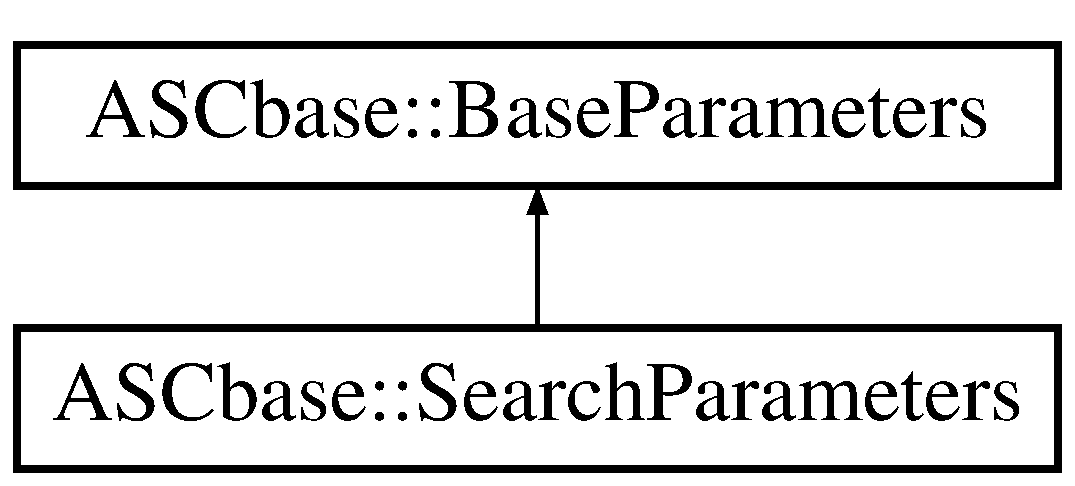
\includegraphics[height=2cm]{classASCbase_1_1SearchParameters}
\end{center}
\end{figure}
\subsection*{Public Types}
\begin{CompactItemize}
\item 
\textbf{PRINT\_\-VERSION} = 1\label{classASCbase_1_1SearchParameters_0278737369e96b0ca8d7685578a160d523d6d6cc3c507f57dbfb27c66de5af61}

\item 
\textbf{PRINT\_\-HELP}\label{classASCbase_1_1SearchParameters_0278737369e96b0ca8d7685578a160d5946fe3b6fb33a3f1a1f1bfcb799e7f57}

\item 
\textbf{DO\_\-NOT\_\-NORMALIZE}\label{classASCbase_1_1SearchParameters_0278737369e96b0ca8d7685578a160d56d064d2864a74b09ebb91ade006be98b}

\item 
\textbf{LIGAND\_\-RMSD}\label{classASCbase_1_1SearchParameters_0278737369e96b0ca8d7685578a160d539c302e55fa4a62c9fc42ddaf0aecf79}

\item 
\textbf{SITEMAP\_\-RMSD}\label{classASCbase_1_1SearchParameters_0278737369e96b0ca8d7685578a160d5be2fcd7debcbc43f9246f2e96a55b061}

\item 
\textbf{DO\_\-NOT\_\-WRITE\_\-LIGANDS}\label{classASCbase_1_1SearchParameters_0278737369e96b0ca8d7685578a160d5842ee3990d6101fe149155fb635857f8}

\item 
\textbf{SCORE\_\-ONLY}\label{classASCbase_1_1SearchParameters_0278737369e96b0ca8d7685578a160d56cca043172e95be1ac3a62aa07b3e929}

\item 
\textbf{DO\_\-NOT\_\-TIME\_\-PROCESS}\label{classASCbase_1_1SearchParameters_0278737369e96b0ca8d7685578a160d5df4956ce18d7222d72380e017a2f08a0}

\item 
\textbf{ALLOW\_\-HPHOB\_\-ONLY\_\-TRIANGLES}\label{classASCbase_1_1SearchParameters_0278737369e96b0ca8d7685578a160d5ff8d9bfbd20c4d153faebdc41c3a6850}

\item 
\textbf{ADD\_\-STRUCT\_\-ID\_\-FIELD}\label{classASCbase_1_1SearchParameters_0278737369e96b0ca8d7685578a160d57ed6e1e5168b8f6cc426662e6d3dcff8}

\item 
\textbf{DO\_\-PROT\_\-LIG\_\-SCORING}\label{classASCbase_1_1SearchParameters_0278737369e96b0ca8d7685578a160d58f07579b71a52c91abe56ecb74b4ff36}

\item 
\textbf{USE\_\-HBOND\_\-SURFACES\_\-MODEL}\label{classASCbase_1_1SearchParameters_0278737369e96b0ca8d7685578a160d5831a2cb95cee561617e96d228eafcedc}

\item 
\textbf{ALLOW\_\-SMALL\_\-SITEMAPS}\label{classASCbase_1_1SearchParameters_0278737369e96b0ca8d7685578a160d543f499df35fbe981319f676f9ed14378}

\item 
\textbf{OMIT\_\-SURFACES}\label{classASCbase_1_1SearchParameters_0278737369e96b0ca8d7685578a160d5e693337097e34cd00710717ddf730bf8}

\item 
\textbf{USE\_\-ONLY\_\-SURFACE\_\-TO\_\-RANK}\label{classASCbase_1_1SearchParameters_0278737369e96b0ca8d7685578a160d53000fed16c2b781a9796124b224878ee}

\item 
\textbf{NO\_\-FINE\_\-TUNING}\label{classASCbase_1_1SearchParameters_0278737369e96b0ca8d7685578a160d5411105460cac2fc65d5266f43736c78f}

\item 
\textbf{FINE\_\-TUNE\_\-TIER2\_\-ALIGNMENTS}\label{classASCbase_1_1SearchParameters_0278737369e96b0ca8d7685578a160d5ecbffd5cf9076e2f4f2d9c596905b669}

\item 
\textbf{FINE\_\-TUNE\_\-BEST\_\-TIER2\_\-ALIGNMENT}\label{classASCbase_1_1SearchParameters_0278737369e96b0ca8d7685578a160d504576ab0c5c8f5dbbba804c2c0274d2a}

\item 
\textbf{SAVE\_\-RIGID\_\-SCORES}\label{classASCbase_1_1SearchParameters_0278737369e96b0ca8d7685578a160d544f84bff804eec7f7c39354f9f8ae626}

\item 
\textbf{CHECK\_\-ALL\_\-TRIANGLES}\label{classASCbase_1_1SearchParameters_0278737369e96b0ca8d7685578a160d50f64c95335dd96cc5921f4fe06da140f}

\item 
\textbf{SCALE\_\-SF\_\-TERMS}\label{classASCbase_1_1SearchParameters_0278737369e96b0ca8d7685578a160d5760e17a2d0988a03d917adef472a93ed}

\item 
\textbf{IK\_\-SURFACES} = 1000\label{classASCbase_1_1SearchParameters_c267aed4ea246dc936ccd5b47b71712d64b3f0cd752f91d46f25e27e791c5bf6}

\item 
\textbf{IK\_\-HB\_\-CAPS}\label{classASCbase_1_1SearchParameters_c267aed4ea246dc936ccd5b47b71712d439d788290c8a2e8caad1e96753d001b}

\item 
\textbf{IK\_\-BOTH\_\-REPS}\label{classASCbase_1_1SearchParameters_c267aed4ea246dc936ccd5b47b71712d1aa6526aee8d82d030cda47ac9831efb}

\item 
enum \textbf{popt\_\-args\_\-t} \{ \par
\textbf{PRINT\_\-VERSION} =  1, 
\textbf{PRINT\_\-HELP}, 
\textbf{DO\_\-NOT\_\-NORMALIZE}, 
\textbf{LIGAND\_\-RMSD}, 
\par
\textbf{SITEMAP\_\-RMSD}, 
\textbf{DO\_\-NOT\_\-WRITE\_\-LIGANDS}, 
\textbf{SCORE\_\-ONLY}, 
\textbf{DO\_\-NOT\_\-TIME\_\-PROCESS}, 
\par
\textbf{ALLOW\_\-HPHOB\_\-ONLY\_\-TRIANGLES}, 
\textbf{ADD\_\-STRUCT\_\-ID\_\-FIELD}, 
\textbf{DO\_\-PROT\_\-LIG\_\-SCORING}, 
\textbf{USE\_\-HBOND\_\-SURFACES\_\-MODEL}, 
\par
\textbf{ALLOW\_\-SMALL\_\-SITEMAPS}, 
\textbf{OMIT\_\-SURFACES}, 
\textbf{USE\_\-ONLY\_\-SURFACE\_\-TO\_\-RANK}, 
\textbf{NO\_\-FINE\_\-TUNING}, 
\par
\textbf{FINE\_\-TUNE\_\-TIER2\_\-ALIGNMENTS}, 
\textbf{FINE\_\-TUNE\_\-BEST\_\-TIER2\_\-ALIGNMENT}, 
\textbf{SAVE\_\-RIGID\_\-SCORES}, 
\textbf{CHECK\_\-ALL\_\-TRIANGLES}, 
\par
\textbf{SCALE\_\-SF\_\-TERMS}
 \}
\item 
enum \textbf{IK\_\-type\_\-t} \{ \textbf{IK\_\-SURFACES} =  1000, 
\textbf{IK\_\-HB\_\-CAPS}, 
\textbf{IK\_\-BOTH\_\-REPS}
 \}
\end{CompactItemize}
\subsection*{Public Member Functions}
\begin{CompactItemize}
\item 
\bf{Search\-Parameters} ()\label{classASCbase_1_1SearchParameters_a08c1e2d66f1c849ba1fb003a6bc6b7f}

\begin{CompactList}\small\item\em To be used by the ASCbase\-Py search.parameters module. \item\end{CompactList}\item 
\bf{Search\-Parameters} (const int argc, const char $\ast$$\ast$argv)\label{classASCbase_1_1SearchParameters_1acc5cc86e0834742971c7a66033c951}

\begin{CompactList}\small\item\em Set the search parameters using the values in argv. \item\end{CompactList}\item 
void \textbf{report\_\-parameters} (std::ostream \&out) const \label{classASCbase_1_1SearchParameters_c3a3ee055bce67d5d055a7a0a939c860}

\end{CompactItemize}
\subsection*{Public Attributes}
\begin{CompactItemize}
\item 
std::string \bf{ext\_\-score\_\-method}\label{classASCbase_1_1SearchParameters_31b913ee478296612756c9b25b34465d}

\begin{CompactList}\small\item\em Name of external scoring method to use. \item\end{CompactList}\item 
std::string \bf{model\_\-file\_\-name}\label{classASCbase_1_1SearchParameters_cdcb30f0c043a4137ed8c790502ada62}

\begin{CompactList}\small\item\em Name of the model points file. \item\end{CompactList}\item 
std::string \bf{dbase\_\-file\_\-name}\label{classASCbase_1_1SearchParameters_c70448bc467a512efafbf3b952770550}

\begin{CompactList}\small\item\em Name of the current dbase points file. \item\end{CompactList}\item 
std::string \bf{ofname}\label{classASCbase_1_1SearchParameters_51c7063e6085b9aa32527a64206ecfdc}

\begin{CompactList}\small\item\em Name of the output file. \item\end{CompactList}\item 
std::string \bf{score\_\-str}\label{classASCbase_1_1SearchParameters_770e3c6ff6ae15a21330d15dcfe3d4d5}

\begin{CompactList}\small\item\em Scoring method. \item\end{CompactList}\item 
std::string \bf{db\_\-index\_\-fname}\label{classASCbase_1_1SearchParameters_48d9df89d360efd9b57b8917aae33712}

\begin{CompactList}\small\item\em Name of database index file. \item\end{CompactList}\item 
int \bf{db\_\-start}\label{classASCbase_1_1SearchParameters_2cd53037b00008f5039381a00085f93d}

\begin{CompactList}\small\item\em Line number of initial db site. \item\end{CompactList}\item 
int \bf{db\_\-stop}\label{classASCbase_1_1SearchParameters_b12f931a64c6d18141bb94cb283c1543}

\begin{CompactList}\small\item\em Line number of final db site. \item\end{CompactList}\item 
bool \bf{normalize}\label{classASCbase_1_1SearchParameters_4265eb5c3b8cd524159bcefd855458fa}

\begin{CompactList}\small\item\em false implies no normalization \item\end{CompactList}\item 
int \bf{num\_\-scores\_\-to\_\-keep}\label{classASCbase_1_1SearchParameters_275f0141e87e686c4c8ee55d9062ae81}

\begin{CompactList}\small\item\em max \# of final alignments to keep for each search sitemap \item\end{CompactList}\item 
int \bf{max\_\-tier1\_\-aligns}\label{classASCbase_1_1SearchParameters_d8fa144982e1f3a459b6797170fec1e9}

\begin{CompactList}\small\item\em max \# of tier1 alignments to pass to tier2 scoring \item\end{CompactList}\item 
my\_\-float\_\-t \bf{score\_\-cutoff}\label{classASCbase_1_1SearchParameters_2ee1752f506f23f99dc8639465c83015}

\begin{CompactList}\small\item\em Keep alignments with score better than cutoff. \item\end{CompactList}\item 
int \bf{min\_\-num\_\-atoms}\label{classASCbase_1_1SearchParameters_b82481de1a76a7e1ef2701225f4e8e2b}

\begin{CompactList}\small\item\em Number of ligand atoms required in query pocket. \item\end{CompactList}\item 
my\_\-float\_\-t \bf{dmetol}\label{classASCbase_1_1SearchParameters_9afa8f1e64a425ad8e45aaf7402029c7}

\begin{CompactList}\small\item\em Tolerance for the average dist. metric error. \item\end{CompactList}\item 
my\_\-float\_\-t \bf{lsetol}\label{classASCbase_1_1SearchParameters_fd82cd2d31ed05774d10ab78235133f6}

\begin{CompactList}\small\item\em Tolerance for the average least squares error. \item\end{CompactList}\item 
bool \textbf{ligand\_\-rmsd}\label{classASCbase_1_1SearchParameters_922b10578a528a00d7b98686005636fe}

\item 
bool \textbf{sitemap\_\-rmsd}\label{classASCbase_1_1SearchParameters_bfcbc6418735f08eb7d0f7bd11d12a62}

\item 
bool \bf{write\_\-ligands}\label{classASCbase_1_1SearchParameters_8f581cefd00526d81c5db9e7f2e53dd7}

\begin{CompactList}\small\item\em True implies write ligands, else do not write. \item\end{CompactList}\item 
bool \bf{align\_\-to\_\-query}\label{classASCbase_1_1SearchParameters_1cb575b033f4db440a377d4ea8332929}

\begin{CompactList}\small\item\em True implies align dbase site to query, else score as given. \item\end{CompactList}\item 
size\_\-t \bf{num\_\-rand\_\-aligns}\label{classASCbase_1_1SearchParameters_019cff6f0e6b9d6028f7e9fab62e62b6}

\begin{CompactList}\small\item\em If not align\_\-to\_\-query, use this many random alignments. \item\end{CompactList}\item 
bool \bf{time\_\-process}\label{classASCbase_1_1SearchParameters_7ed54b1f8513ddd3e56686c36fb0f89d}

\begin{CompactList}\small\item\em If true, use itimers to time program. \item\end{CompactList}\item 
bool \bf{allow\_\-hphob\_\-triangles}\label{classASCbase_1_1SearchParameters_a9d1bb630cda4fe759f4299354cef05f}

\begin{CompactList}\small\item\em If false, triangle need at least 1 hbond. \item\end{CompactList}\item 
bool \bf{add\_\-struct\_\-id\_\-field}\label{classASCbase_1_1SearchParameters_6dbd7bf284c1dbfd2c2af2becf89a078}

\begin{CompactList}\small\item\em If false \& empty pockets searches, write struct id into ligand field for empty pocket hits. \item\end{CompactList}\item 
bool \bf{do\_\-internal\_\-prot\_\-lig\_\-score}\label{classASCbase_1_1SearchParameters_96a5af359501d56a5670d49c32467994}

\begin{CompactList}\small\item\em If true compute affi and orient score for query prot and db lig interactions. \item\end{CompactList}\item 
bool \bf{use\_\-hbond\_\-surfaces}\label{classASCbase_1_1SearchParameters_1c517ad691e1606cce4cdfac986067b0}

\begin{CompactList}\small\item\em If true, use the hbond surfaces modeling of hydrogen bonding regions (volumes). \item\end{CompactList}\item 
bool \bf{fine\_\-tune\_\-tier2\_\-alignments}\label{classASCbase_1_1SearchParameters_7e249d3358f464048cca7f574052e844}

\begin{CompactList}\small\item\em If true, use an ICP like method to fine tune all tier2 alignments. \item\end{CompactList}\item 
bool \bf{fine\_\-tune\_\-best\_\-tier2\_\-alignment}\label{classASCbase_1_1SearchParameters_6c449d3293b369f0c71e875e14d2039a}

\begin{CompactList}\small\item\em If true, use an ICP-like method to fine tune the best scoring tier2 alignment. \item\end{CompactList}\item 
bool \bf{check\_\-all\_\-triangles}\label{classASCbase_1_1SearchParameters_44592b748c47ab06a54c680635dc0795}

\begin{CompactList}\small\item\em If true, check all triangles in dbase mesh for closest point to each query vertex -- useful for testing. \item\end{CompactList}\item 
std::string \bf{query\_\-prot}\label{classASCbase_1_1SearchParameters_600f1a2e9136a1c54dc751c3bc6f3665}

\begin{CompactList}\small\item\em Currently required for hbond\_\-surfaces. \item\end{CompactList}\item 
bool \bf{save\_\-rigid\_\-scores}\label{classASCbase_1_1SearchParameters_bc80a6f5d0264c5f4b5ca582c1183a14}

\begin{CompactList}\small\item\em When using ICP, save the rigid scores to another output file. \item\end{CompactList}\item 
bool \bf{scale\_\-terms}\label{classASCbase_1_1SearchParameters_dcb623f26a6aabaf855021f954cee078}

\begin{CompactList}\small\item\em If true, scale each term of the scoring function(s) linearly from [0.0, max] to [0.0, 1.0] where max is the max value the query site can have for that term. \item\end{CompactList}\item 
bool \textbf{do\_\-IK}\label{classASCbase_1_1SearchParameters_ae98a5075be2f4c92734f47223076e6c}

\item 
my\_\-float\_\-t \bf{max\_\-corr\_\-surf\_\-pt\_\-dist}\label{classASCbase_1_1SearchParameters_ac2413e22df6100db6b73f5920cc9ddd}

\begin{CompactList}\small\item\em Maximum distance to consider corresponding surface points. \item\end{CompactList}\item 
my\_\-float\_\-t \bf{fine\_\-tune\_\-ratio}\label{classASCbase_1_1SearchParameters_62849cae5f51eb12263a341056af66c5}

\begin{CompactList}\small\item\em Ratio of shape point weight (msms surf) to hbond cap point weight (1.0 imples equal, 2.0 implies surface points get weighted twice that of hbond caps, etc.) Default is Zero, which implies use only the MSMS surface for ICP. \item\end{CompactList}\item 
std::string \bf{alignments\_\-fname}\label{classASCbase_1_1SearchParameters_5a36fe41006109a902194d9e2cf39e1a}

\begin{CompactList}\small\item\em Path to alignments file (in Sim\-Site3D results file format with at least 4 fields per line -- struct\_\-id, score, R, T; and in that order and pipe delimited fields with numbers single space delimited). \item\end{CompactList}\item 
IK\_\-type\_\-t \bf{IK\_\-type}\label{classASCbase_1_1SearchParameters_84a374fa89c1f6d5868a830091d2178c}

\begin{CompactList}\small\item\em Type of IK method to use. \item\end{CompactList}\end{CompactItemize}
\subsection*{Private Member Functions}
\begin{CompactItemize}
\item 
void \textbf{init\_\-vars} ()\label{classASCbase_1_1SearchParameters_0b3092dc843090100b6d8707f438ff82}

\item 
void \textbf{free\_\-cstrings} ()\label{classASCbase_1_1SearchParameters_c5be044fd7c950fbf1b3472d01e9c0f5}

\item 
status\_\-t \textbf{get\_\-opts} (const int argc, const char $\ast$$\ast$argv)\label{classASCbase_1_1SearchParameters_e7af633b8fc93087ddf5067551929741}

\item 
status\_\-t \textbf{verify\_\-parameters} ()\label{classASCbase_1_1SearchParameters_cc0d8f138dd11fa98a0fa52c59f1a9b2}

\end{CompactItemize}
\subsection*{Private Attributes}
\begin{CompactItemize}
\item 
char $\ast$ \bf{A\_\-conf\_\-fname}\label{classASCbase_1_1SearchParameters_3cb03731b1e4917864cade8bb39d7f95}

\begin{CompactList}\small\item\em Location of environment configure file. \item\end{CompactList}\item 
char $\ast$ \bf{A\_\-proj\_\-output}\label{classASCbase_1_1SearchParameters_b89a1895609e2d782727d5b81e70fff4}

\begin{CompactList}\small\item\em Directory to store results. \item\end{CompactList}\item 
char $\ast$ \bf{A\_\-scratch\_\-dir}\label{classASCbase_1_1SearchParameters_27e0256e5782174a8a5da589e84ef6da}

\begin{CompactList}\small\item\em Directory to use as a scratch space. \item\end{CompactList}\item 
char $\ast$ \bf{A\_\-dbase\_\-dir}\label{classASCbase_1_1SearchParameters_2cbe4df7b590f7cb0fff7584fcecf59b}

\begin{CompactList}\small\item\em Location of the database to query. \item\end{CompactList}\item 
char $\ast$ \bf{A\_\-ligs\_\-dir}\label{classASCbase_1_1SearchParameters_3dc1434fb48a7773cbe4fd247a87de77}

\begin{CompactList}\small\item\em Location of ligands associated with dbase\_\-dir. \item\end{CompactList}\end{CompactItemize}
\subsection*{Static Private Attributes}
\begin{CompactItemize}
\item 
static const std::string \bf{A\_\-fname} = \char`\"{}Search\-Parameters.C\char`\"{}\label{classASCbase_1_1SearchParameters_865031ac44a12f4833a96bf17e718b2c}

\begin{CompactList}\small\item\em Name of the source file. \item\end{CompactList}\end{CompactItemize}


\subsection{Detailed Description}
Use popt to parse a search's commandline parameters. 



The documentation for this class was generated from the following files:\begin{CompactItemize}
\item 
Search\-Parameters.H\item 
Search\-Parameters.C\end{CompactItemize}

\section{ASCbase::SFCscore\-Interface Class Reference}
\label{classASCbase_1_1SFCscoreInterface}\index{ASCbase::SFCscoreInterface@{ASCbase::SFCscoreInterface}}
Wrapper and parser for the external scoring functions in SFCscore.  


{\tt \#include $<$SFCscore\-Interface.H$>$}

Inheritance diagram for ASCbase::SFCscore\-Interface::\begin{figure}[H]
\begin{center}
\leavevmode
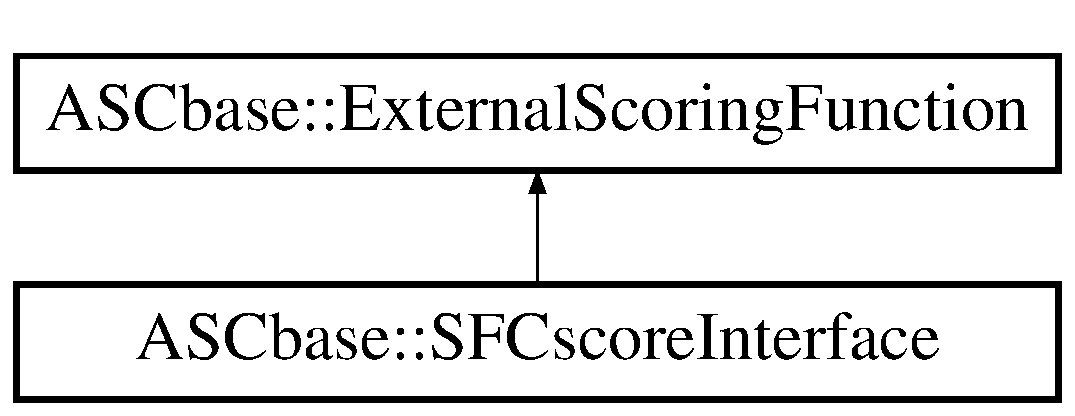
\includegraphics[height=2cm]{classASCbase_1_1SFCscoreInterface}
\end{center}
\end{figure}
\subsection*{Public Member Functions}
\begin{CompactItemize}
\item 
\bf{SFCscore\-Interface} (std::string cmdline)
\begin{CompactList}\small\item\em Constructor. \item\end{CompactList}\item 
\bf{$\sim$SFCscore\-Interface} ()\label{classASCbase_1_1SFCscoreInterface_a845154d606be294b33e129f424fffee}

\begin{CompactList}\small\item\em Do nothing destructor. \item\end{CompactList}\item 
bool \bf{score} (std::string prot\_\-path, std::string lig\_\-path, std::vector$<$ my\_\-float\_\-t $>$ $\ast$scores)
\begin{CompactList}\small\item\em Wrapper to \doxyref{External\-Scoring\-Function::run}{p.}{classASCbase_1_1ExternalScoringFunction_118e501c983ee3c61747b40741c776ff} and parse output score file. \item\end{CompactList}\item 
void \bf{sf\_\-names} (std::vector$<$ std::string $>$ $\ast$names)
\begin{CompactList}\small\item\em Get a list of the scoring functions calculated by SFCscore. \item\end{CompactList}\end{CompactItemize}
\subsection*{Private Member Functions}
\begin{CompactItemize}
\item 
bool \bf{get\_\-scoring\_\-functions} (std::string spf\_\-fname)
\begin{CompactList}\small\item\em Get the names of the scoring functions in the .spf file. \item\end{CompactList}\end{CompactItemize}
\subsection*{Private Attributes}
\begin{CompactItemize}
\item 
std::vector$<$ std::string $>$ \bf{sfc\_\-names}\label{classASCbase_1_1SFCscoreInterface_f5e8e5ccda0fe051ec010930c9145036}

\begin{CompactList}\small\item\em Vector holding names of SFC scoring functions requested in the spf file. \item\end{CompactList}\end{CompactItemize}
\subsection*{Static Private Attributes}
\begin{CompactItemize}
\item 
static const std::string \bf{\_\-fname} = \char`\"{}SFCscore\-Interface.C\char`\"{}\label{classASCbase_1_1SFCscoreInterface_98919969ba57e3e42b90acb6be87344f}

\begin{CompactList}\small\item\em \char`\"{}SFCscore\-Interface.C\char`\"{} \item\end{CompactList}\end{CompactItemize}


\subsection{Detailed Description}
Wrapper and parser for the external scoring functions in SFCscore. 

This is a hack to get SFCscore to work with ASCbase. At present, running with a specified weight file is not supported (by ASCbase; i.e. this class) 



\subsection{Constructor \& Destructor Documentation}
\index{ASCbase::SFCscoreInterface@{ASCbase::SFCscore\-Interface}!SFCscoreInterface@{SFCscoreInterface}}
\index{SFCscoreInterface@{SFCscoreInterface}!ASCbase::SFCscoreInterface@{ASCbase::SFCscore\-Interface}}
\subsubsection{\setlength{\rightskip}{0pt plus 5cm}SFCscore\-Interface::SFCscore\-Interface (std::string {\em cmdline})}\label{classASCbase_1_1SFCscoreInterface_3ce57c925d03cb064b4360006f2aded7}


Constructor. 

\begin{Desc}
\item[Parameters:]
\begin{description}
\item[{\em cmdline}]String holding the SFCscore command line \end{description}
\end{Desc}


\subsection{Member Function Documentation}
\index{ASCbase::SFCscoreInterface@{ASCbase::SFCscore\-Interface}!get_scoring_functions@{get\_\-scoring\_\-functions}}
\index{get_scoring_functions@{get\_\-scoring\_\-functions}!ASCbase::SFCscoreInterface@{ASCbase::SFCscore\-Interface}}
\subsubsection{\setlength{\rightskip}{0pt plus 5cm}bool SFCscore\-Interface::get\_\-scoring\_\-functions (std::string {\em spf\_\-fname})\hspace{0.3cm}{\tt  [private]}}\label{classASCbase_1_1SFCscoreInterface_f137ba2029c31c5344839b3e1862a1c4}


Get the names of the scoring functions in the .spf file. 

Given the .spf file as passed to the constructor, parse the file looking for the line starting with \char`\"{}SCORE\char`\"{} (no preceeding spaces). The listed scoring functions will be used to determine the files to parse and list in the score listing (report).

\begin{Desc}
\item[Parameters:]
\begin{description}
\item[{\em spf\_\-fname}]Path to the .spf file--typically specified in the options field of the ASCbase\-Soft\-Params/external\_\-scoring\_\-functions.txt file \end{description}
\end{Desc}
\begin{Desc}
\item[Returns:]True if the .spf file was opened for reading, otherwise false \end{Desc}
\index{ASCbase::SFCscoreInterface@{ASCbase::SFCscore\-Interface}!score@{score}}
\index{score@{score}!ASCbase::SFCscoreInterface@{ASCbase::SFCscore\-Interface}}
\subsubsection{\setlength{\rightskip}{0pt plus 5cm}bool SFCscore\-Interface::score (std::string {\em prot\_\-path}, std::string {\em lig\_\-path}, std::vector$<$ my\_\-float\_\-t $>$ $\ast$ {\em scores})\hspace{0.3cm}{\tt  [virtual]}}\label{classASCbase_1_1SFCscoreInterface_354838006d3b086f93b7245cf0223a70}


Wrapper to \doxyref{External\-Scoring\-Function::run}{p.}{classASCbase_1_1ExternalScoringFunction_118e501c983ee3c61747b40741c776ff} and parse output score file. 

\begin{Desc}
\item[Parameters:]
\begin{description}
\item[{\em prot\_\-path}]String holding the path of the protein PDB file \item[{\em lig\_\-path}]String holding the path of the ligand mol2 file  scores Pointer to vector to hold the score(s) from SFCscore \end{description}
\end{Desc}
\begin{Desc}
\item[Returns:]True if SFCscore seemed to work, otherwise false \end{Desc}


Implements \bf{ASCbase::External\-Scoring\-Function} \doxyref{p.}{classASCbase_1_1ExternalScoringFunction_d0e70f7569b5746af85eebc1208afa2a}.\index{ASCbase::SFCscoreInterface@{ASCbase::SFCscore\-Interface}!sf_names@{sf\_\-names}}
\index{sf_names@{sf\_\-names}!ASCbase::SFCscoreInterface@{ASCbase::SFCscore\-Interface}}
\subsubsection{\setlength{\rightskip}{0pt plus 5cm}void SFCscore\-Interface::sf\_\-names (std::vector$<$ std::string $>$ $\ast$ {\em names})\hspace{0.3cm}{\tt  [virtual]}}\label{classASCbase_1_1SFCscoreInterface_00c2a69a8732cc3eae24ed2bb61dc638}


Get a list of the scoring functions calculated by SFCscore. 

Get the scoring functions listed in the .spf file.

\begin{Desc}
\item[Parameters:]
\begin{description}
\item[{\em name}]Pointer to vector of strings to hold the names of the scoring functions listed in the .spf file \end{description}
\end{Desc}


Implements \bf{ASCbase::External\-Scoring\-Function} \doxyref{p.}{classASCbase_1_1ExternalScoringFunction_3db07e1e70e4946b507c9b320a124b8b}.

The documentation for this class was generated from the following files:\begin{CompactItemize}
\item 
SFCscore\-Interface.H\item 
SFCscore\-Interface.C\end{CompactItemize}

\section{Simple\-Octree$<$ \_\-Tp $>$ Class Template Reference}
\label{classSimpleOctree}\index{SimpleOctree@{SimpleOctree}}
Simple \doxyref{Octree}{p.}{classOctree} for any datatype with an associated 3D position.  


{\tt \#include $<$Simple\-Octree.H$>$}

\subsection*{Public Member Functions}
\begin{CompactItemize}
\item 
\textbf{Simple\-Octree} (const my\_\-float\_\-t min\_\-half\_\-width, const uint max\_\-numel=1)\label{classSimpleOctree_c660f5f62e287615994fb741588c3b46}

\item 
void \textbf{build} (\_\-Tp pts\_\-begin, \_\-Tp pts\_\-end)\label{classSimpleOctree_339dae8210f68be58b801fdf3e68cdd7}

\item 
void \textbf{subdivide\_\-with\_\-overlap} (octree\_\-node\_\-t$<$ \_\-Tp $>$ $\ast$cnode)\label{classSimpleOctree_6396158ba3432b3f0940c73af34e2143}

\item 
const std::vector$<$ \_\-Tp $>$ $\ast$ \textbf{near\_\-by\_\-points} (const my\_\-float\_\-t $\ast$pos, const my\_\-float\_\-t max\_\-dist)\label{classSimpleOctree_6f5f1e2bc6990bf849d8636b1274c125}

\item 
void \bf{bin\_\-positions} (const std::vector$<$ const my\_\-float\_\-t $\ast$ $>$ \&pos\_\-vec, const my\_\-float\_\-t max\_\-dist, std::vector$<$ bin\_\-type $>$ $\ast$bins)
\end{CompactItemize}
\subsection*{Private Types}
\begin{CompactItemize}
\item 
typedef \_\-Tp \textbf{value\_\-type}\label{classSimpleOctree_a1cd7fcefdc87bd36c117b7cc59cf4f3}

\end{CompactItemize}
\subsection*{Private Member Functions}
\begin{CompactItemize}
\item 
void \textbf{bin\_\-positions} (octree\_\-node\_\-t$<$ \_\-Tp $>$ \&cnode, const my\_\-float\_\-t max\_\-dist, const std::vector$<$ const my\_\-float\_\-t $\ast$ $>$ \&pos\_\-vec, std::vector$<$ bin\_\-type $>$ $\ast$bins)\label{classSimpleOctree_d81f6ed6df7e0dee530e118be1f7eaae}

\end{CompactItemize}
\subsection*{Private Attributes}
\begin{CompactItemize}
\item 
octree\_\-node\_\-t$<$ \_\-Tp $>$ \bf{A\_\-root}\label{classSimpleOctree_20d500a92872180e646c24ce8b74cd47}

\begin{CompactList}\small\item\em Root node of the tree. \item\end{CompactList}\item 
uint \bf{A\_\-max\_\-numel}\label{classSimpleOctree_4b7ee1b029f49a644e1b31101eafc617}

\begin{CompactList}\small\item\em Max number of elements in a cube at a level less than the max level. \item\end{CompactList}\item 
my\_\-float\_\-t \bf{A\_\-min\_\-half\_\-width}\label{classSimpleOctree_bc63a507b42604835d4014ee866080a8}

\begin{CompactList}\small\item\em Smallest cube should be about this size. \item\end{CompactList}\end{CompactItemize}
\subsection*{Static Private Attributes}
\begin{CompactItemize}
\item 
static const std::string \bf{A\_\-fname}\label{classSimpleOctree_2e0789a304beb91d4a9901d3a92da94a}

\begin{CompactList}\small\item\em Name of the source file. \item\end{CompactList}\end{CompactItemize}
\subsection*{Classes}
\begin{CompactItemize}
\item 
struct \textbf{bin\_\-type}
\end{CompactItemize}


\subsection{Detailed Description}
\subsubsection*{template$<$typename \_\-Tp$>$ class Simple\-Octree$<$ \_\-Tp $>$}

Simple \doxyref{Octree}{p.}{classOctree} for any datatype with an associated 3D position. 

It is reasonably efficient when compared with brute force, but a few more checks and the number of returned points, etc would be reduced further. 



\subsection{Member Function Documentation}
\index{SimpleOctree@{Simple\-Octree}!bin_positions@{bin\_\-positions}}
\index{bin_positions@{bin\_\-positions}!SimpleOctree@{Simple\-Octree}}
\subsubsection{\setlength{\rightskip}{0pt plus 5cm}template$<$typename \_\-Tp$>$ void \bf{Simple\-Octree}$<$ \_\-Tp $>$::bin\_\-positions (const std::vector$<$ const my\_\-float\_\-t $\ast$ $>$ \& {\em pos\_\-vec}, const my\_\-float\_\-t {\em max\_\-dist}, std::vector$<$ bin\_\-type $>$ $\ast$ {\em bins})\hspace{0.3cm}{\tt  [inline]}}\label{classSimpleOctree_deae8a2d70769960c5492b2a5abaf52d}


This function was not tested enough and it should also be timed to check if it is really any faster than near\_\-by\_\-points for each point 

The documentation for this class was generated from the following file:\begin{CompactItemize}
\item 
Simple\-Octree.H\end{CompactItemize}

\section{ASCbase::Simple\-Trimesh Class Reference}
\label{classASCbase_1_1SimpleTrimesh}\index{ASCbase::SimpleTrimesh@{ASCbase::SimpleTrimesh}}
{\tt \#include $<$Simple\-Trimesh.H$>$}

\subsection*{Public Types}
\begin{CompactItemize}
\item 
typedef std::multimap$<$ my\_\-float\_\-t, correspond\_\-t $>$ \textbf{correspond\_\-map}\label{classASCbase_1_1SimpleTrimesh_2ca3d7877ebea7cd14caed7b69916786}

\item 
typedef correspond\_\-map::const\_\-iterator \textbf{correspond\_\-mmci}\label{classASCbase_1_1SimpleTrimesh_cf7601a2bd1e9a025743c55b2c41db20}

\item 
typedef std::vector$<$ triangle\_\-t $>$ \textbf{face\_\-vec}\label{classASCbase_1_1SimpleTrimesh_abdd82d831b014f4e94e2af71ab8ae7a}

\item 
typedef face\_\-vec::const\_\-iterator \textbf{face\_\-vci}\label{classASCbase_1_1SimpleTrimesh_b4de70c1cdbd9ce9d95ccf9d0986b7e1}

\end{CompactItemize}
\subsection*{Public Member Functions}
\begin{CompactItemize}
\item 
\textbf{Simple\-Trimesh} (const std::string fname, bool check\_\-vertex\_\-order=false)\label{classASCbase_1_1SimpleTrimesh_3e3d62990f6adc85a2f7773896c92f34}

\item 
\textbf{Simple\-Trimesh} (\bf{Simple\-Trimesh} \&src, \bf{Bounding\-Volume} \&bvol)\label{classASCbase_1_1SimpleTrimesh_8abd29eec3ba76a51d59835e465a35ee}

\item 
\textbf{Simple\-Trimesh} (\bf{Simple\-Trimesh} \&src, const my\_\-float\_\-t $\ast$center, const my\_\-float\_\-t radius)\label{classASCbase_1_1SimpleTrimesh_ef4ffdf1fd937f5209f81d9f58e9b1a9}

\item 
void \textbf{clip} (const my\_\-float\_\-t $\ast$center, const my\_\-float\_\-t radius)\label{classASCbase_1_1SimpleTrimesh_6589c1db21145564e4d1e6de26e77060}

\item 
void \textbf{intersect} (const \bf{Bounding\-Volume} $\ast$bvol)\label{classASCbase_1_1SimpleTrimesh_db13b6eab9e030cf21c594f2d0613051}

\item 
bool \textbf{write} (const std::string ofname) const \label{classASCbase_1_1SimpleTrimesh_4d5fc687d60362490263ef26eade8fbb}

\item 
my\_\-float\_\-t \textbf{get\_\-total\_\-SA} () const \label{classASCbase_1_1SimpleTrimesh_fd2c1d5f6be4c731c4b64ec249f6f1ef}

\item 
bool \textbf{old\_\-compare} (const \bf{Simple\-Trimesh} \&target, const my\_\-float\_\-t max\_\-pt\_\-dist, size\_\-t $\ast$num\_\-points, my\_\-float\_\-t $\ast$RMSE, size\_\-t $\ast$num\_\-faces=0, my\_\-float\_\-t $\ast$area=0) const \label{classASCbase_1_1SimpleTrimesh_c55aa8f87f4244a93cc319220815b2c1}

\item 
void \textbf{compare} (const \bf{Simple\-Trimesh} \&target, const my\_\-float\_\-t max\_\-pt\_\-dist, size\_\-t $\ast$num\_\-points, my\_\-float\_\-t $\ast$RMSE, correspond\_\-map $\ast$cmap=0, size\_\-t $\ast$num\_\-faces=0, my\_\-float\_\-t $\ast$area=0) const \label{classASCbase_1_1SimpleTrimesh_0674ac20bbafd3d2ce88edbf010cb83b}

\item 
void \textbf{transform} (const my\_\-float\_\-t $\ast$R, const my\_\-float\_\-t $\ast$T)\label{classASCbase_1_1SimpleTrimesh_62c0d274f674d05c9db0ca18aea2db11}

\item 
void \textbf{inverse\_\-transform} (const my\_\-float\_\-t $\ast$R, const my\_\-float\_\-t $\ast$T)\label{classASCbase_1_1SimpleTrimesh_5a59c678cf6712f29f796144cf8c87de}

\item 
void \textbf{revert} ()\label{classASCbase_1_1SimpleTrimesh_5310633ed75943845498b55b60793de5}

\item 
const my\_\-float\_\-t $\ast$ \textbf{vertices\_\-begin} () const \label{classASCbase_1_1SimpleTrimesh_0241ee914bc4009b298dcbf4f8509b0c}

\item 
std::vector$<$ triangle\_\-t $>$::const\_\-iterator \textbf{faces\_\-begin} () const \label{classASCbase_1_1SimpleTrimesh_a3884b72a389a2db888fdbfe87e9d18b}

\item 
std::vector$<$ triangle\_\-t $>$::const\_\-iterator \textbf{faces\_\-end} () const \label{classASCbase_1_1SimpleTrimesh_f460bb83919675913193bb8271b65b53}

\item 
size\_\-t \textbf{number\_\-of\_\-vertices} () const \label{classASCbase_1_1SimpleTrimesh_e5fa28939fe7b60139c77490226b7c19}

\item 
size\_\-t \textbf{number\_\-of\_\-faces} () const \label{classASCbase_1_1SimpleTrimesh_fb3840ef015be2eba2295d7527241687}

\item 
bool \textbf{fail} () const \label{classASCbase_1_1SimpleTrimesh_851505ebe0adff90db508c9f3f0e467f}

\item 
void \textbf{build\_\-vert\_\-face\_\-map} ()\label{classASCbase_1_1SimpleTrimesh_ec6e3af8fdf30ae9975017c727922700}

\item 
void \bf{build\_\-vert\_\-octree} ()\label{classASCbase_1_1SimpleTrimesh_e7086080fb8f55f239829a61ba081c21}

\begin{CompactList}\small\item\em To be called from the query sitemap. \item\end{CompactList}\end{CompactItemize}
\subsection*{Private Types}
\begin{CompactItemize}
\item 
typedef std::map$<$ const my\_\-float\_\-t $\ast$, pt\_\-plus\_\-dist $>$ \textbf{corr\_\-map}\label{classASCbase_1_1SimpleTrimesh_34f4df8be6ca27f3e8cd41c636ddbbde}

\item 
typedef std::map$<$ const my\_\-float\_\-t $\ast$, std::vector$<$ face\_\-vci $>$ $>$ \textbf{vert\_\-face\_\-map}\label{classASCbase_1_1SimpleTrimesh_00a413368aebdc035ace7e9327937c48}

\item 
typedef vert\_\-face\_\-map::iterator \textbf{vert\_\-face\_\-mi}\label{classASCbase_1_1SimpleTrimesh_2fa87e7c069e562d1761244b644fa746}

\item 
typedef vert\_\-face\_\-map::const\_\-iterator \textbf{vert\_\-face\_\-mci}\label{classASCbase_1_1SimpleTrimesh_0975a32279b1889f5a04d8d8613b28a6}

\end{CompactItemize}
\subsection*{Private Member Functions}
\begin{CompactItemize}
\item 
void \textbf{init} ()\label{classASCbase_1_1SimpleTrimesh_0e5578ec2f86102a488219ec4765636c}

\item 
bool \textbf{read\_\-vert\_\-file} (const std::string fname)\label{classASCbase_1_1SimpleTrimesh_817b22c2555bee30b2c3a08669e3ba46}

\item 
bool \textbf{read\_\-face\_\-file} (const std::string fname, bool check\_\-vertex\_\-order)\label{classASCbase_1_1SimpleTrimesh_45339d3843bd2b4c17ad571eb3622a9c}

\item 
size\_\-t \textbf{intersect} (\bf{Bounding\-Volume} \&bvol, size\_\-t $\ast$new\_\-num\_\-verts, my\_\-float\_\-t $\ast$$\ast$new\_\-vertices, my\_\-float\_\-t $\ast$$\ast$new\_\-normals, std::vector$<$ triangle\_\-t $>$ $\ast$new\_\-faces)\label{classASCbase_1_1SimpleTrimesh_e63a3ebc10e0983b60504e799992d7c6}

\item 
size\_\-t \textbf{clip} (const my\_\-float\_\-t $\ast$center, const my\_\-float\_\-t radius, size\_\-t $\ast$new\_\-num\_\-verts, my\_\-float\_\-t $\ast$$\ast$new\_\-vertices, my\_\-float\_\-t $\ast$$\ast$new\_\-normals, std::vector$<$ triangle\_\-t $>$ $\ast$new\_\-faces)\label{classASCbase_1_1SimpleTrimesh_8dc60bdfb5cd7102b5fe52ed0a2afb31}

\item 
void \textbf{copy\_\-kept} (std::map$<$ const my\_\-float\_\-t $\ast$, locations $>$ \&V\_\-keep, my\_\-float\_\-t $\ast$$\ast$new\_\-vertices, my\_\-float\_\-t $\ast$$\ast$new\_\-normals, std::vector$<$ triangle\_\-t $>$ $\ast$new\_\-faces)\label{classASCbase_1_1SimpleTrimesh_a584badfab426f5b183a103b4082186b}

\item 
void \textbf{compute\_\-areas} ()\label{classASCbase_1_1SimpleTrimesh_7ae5091189436be2401d74ada2f49349}

\end{CompactItemize}
\subsection*{Private Attributes}
\begin{CompactItemize}
\item 
size\_\-t \textbf{A\_\-num\_\-verts}\label{classASCbase_1_1SimpleTrimesh_6a22833ec49ae22b4bcae565ab506ee7}

\item 
my\_\-float\_\-t $\ast$ \textbf{A\_\-vertices}\label{classASCbase_1_1SimpleTrimesh_0b2728defec0b9891a7d0994e18409a5}

\item 
my\_\-float\_\-t $\ast$ \textbf{A\_\-normals}\label{classASCbase_1_1SimpleTrimesh_ad00478d9a636db9bfebaaa231af324a}

\item 
my\_\-float\_\-t $\ast$ \textbf{A\_\-original\_\-vertices}\label{classASCbase_1_1SimpleTrimesh_f6d1e2ff40b5128807071b875f9ed5a3}

\item 
my\_\-float\_\-t $\ast$ \textbf{A\_\-original\_\-normals}\label{classASCbase_1_1SimpleTrimesh_8b4de78334d1f9d9000736d1a4dd136b}

\item 
face\_\-vec \textbf{A\_\-triangles}\label{classASCbase_1_1SimpleTrimesh_5c348cc0d69688bc23fabb76b264761f}

\item 
vert\_\-face\_\-map \textbf{A\_\-map\_\-vert\_\-to\_\-faces}\label{classASCbase_1_1SimpleTrimesh_a32acc842c22b1302bde419ff1d5eb5a}

\item 
point\_\-vec\_\-t \textbf{A\_\-vert\_\-vector}\label{classASCbase_1_1SimpleTrimesh_26be812cfc1a68392a84acff308cb0d1}

\item 
\bf{Simple\-Octree}$<$ point\_\-vci $>$ $\ast$ \textbf{A\_\-vert\_\-octree}\label{classASCbase_1_1SimpleTrimesh_00784171656f6854854ac59e66946560}

\item 
bool \textbf{A\_\-fail}\label{classASCbase_1_1SimpleTrimesh_06ae2ea910eb94d50838f28e88b39949}

\end{CompactItemize}
\subsection*{Static Private Attributes}
\begin{CompactItemize}
\item 
static const std::string \textbf{A\_\-fname} = \char`\"{}Simple\-Trimesh.C\char`\"{}\label{classASCbase_1_1SimpleTrimesh_280c7e3491eb35295f8f5bd38e2213d5}

\end{CompactItemize}
\subsection*{Classes}
\begin{CompactItemize}
\item 
struct \textbf{correspond\_\-t}
\item 
struct \textbf{locations}
\item 
struct \textbf{pt\_\-plus\_\-dist}
\item 
struct \textbf{triangle\_\-t}
\end{CompactItemize}


\subsection{Detailed Description}
Simple surface class built for speed of computing the shortest point to surface distance. 



The documentation for this class was generated from the following files:\begin{CompactItemize}
\item 
Simple\-Trimesh.H\item 
Simple\-Trimesh.C\end{CompactItemize}

\section{ASCbase::geometry::Simple\-Trimesh\-Three Class Reference}
\label{classASCbase_1_1geometry_1_1SimpleTrimeshThree}\index{ASCbase::geometry::SimpleTrimeshThree@{ASCbase::geometry::SimpleTrimeshThree}}
Simple surface class built to contain basic features of a triangle mesh.  


{\tt \#include $<$Simple\-Trimesh\-Three.H$>$}

\subsection*{Public Member Functions}
\begin{CompactItemize}
\item 
\bf{Simple\-Trimesh\-Three} ()\label{classASCbase_1_1geometry_1_1SimpleTrimeshThree_188f1d854a84a1bc43b93ba69732ead9}

\begin{CompactList}\small\item\em Default constructor -- initializes some class variables. \item\end{CompactList}\item 
bool \textbf{read\_\-vert\_\-file} (const std::string fname, const bool sample\_\-surface=false)\label{classASCbase_1_1geometry_1_1SimpleTrimeshThree_c9550b4265e3c6cdcaf8cb7ef4240421}

\item 
bool \textbf{read\_\-face\_\-file} (const std::string fname, std::vector$<$ Edge $>$ $\ast$edges, const bool check\_\-vertex\_\-order, const bool compute\_\-max\_\-dist\_\-to\_\-centroid)\label{classASCbase_1_1geometry_1_1SimpleTrimeshThree_a2eef2ac284240c555bc43308012e375}

\item 
const bool \bf{fail} () const 
\item 
const size\_\-t \textbf{num\_\-verts} () const \label{classASCbase_1_1geometry_1_1SimpleTrimeshThree_7357eadf46a005993e7bb4cb1525b3e7}

\item 
void \bf{initialize\_\-opt} (std::vector$<$ Edge $>$ \&edges)
\item 
const my\_\-float\_\-t \textbf{max\_\-dist\_\-to\_\-centroid} () const \label{classASCbase_1_1geometry_1_1SimpleTrimeshThree_623a310518c90b27345b436082e5d5dc}

\item 
\bf{Vert\-Attrib::vci} \textbf{vertices\_\-begin} () const \label{classASCbase_1_1geometry_1_1SimpleTrimeshThree_e80531bbf6af55529137b553dc205a61}

\item 
\bf{Vert\-Attrib::vci} \textbf{vertices\_\-end} () const \label{classASCbase_1_1geometry_1_1SimpleTrimeshThree_a45c5de311686b10920adbdb4ede817a}

\item 
\bf{Face\-Attrib::vci} \textbf{faces\_\-begin} () const \label{classASCbase_1_1geometry_1_1SimpleTrimeshThree_647b6b8412d82b702e5fe4b07ecf07d9}

\item 
\bf{Face\-Attrib::vci} \textbf{faces\_\-end} () const \label{classASCbase_1_1geometry_1_1SimpleTrimeshThree_daf2e57ad4a17d02afaa8e62da5e2ce2}

\end{CompactItemize}
\subsection*{Protected Member Functions}
\begin{CompactItemize}
\item 
void \textbf{set\_\-fail\_\-flag} ()\label{classASCbase_1_1geometry_1_1SimpleTrimeshThree_0aee50a52a6b7dd7eb12de42e516f724}

\end{CompactItemize}
\subsection*{Private Member Functions}
\begin{CompactItemize}
\item 
bool \bf{get\_\-faces} (const \bf{Vert\-Attrib::vi} \&central\_\-vert, const \bf{Face\-Attrib::vi} \&start\_\-face, std::vector$<$ \bf{Face\-Attrib::vi} $>$ $\ast$faces\_\-out, const bool skip\_\-first\_\-prev=false)
\begin{CompactList}\small\item\em Get all the faces for the given vertex. \item\end{CompactList}\item 
void \bf{get\_\-faces} (const Edge \&E, std::vector$<$ \bf{Face\-Attrib::vi} $>$ $\ast$faces\_\-out)\label{classASCbase_1_1geometry_1_1SimpleTrimeshThree_b02e426e7faeba41f1b1814692130246}

\begin{CompactList}\small\item\em This method will fail in the case of a \char`\"{}bad\char`\"{} mesh. \item\end{CompactList}\item 
bool \textbf{get\_\-faces} (\bf{Face\-Attrib::vi} central\_\-face, std::vector$<$ \bf{Face\-Attrib::vi} $>$ $\ast$faces\_\-out)\label{classASCbase_1_1geometry_1_1SimpleTrimeshThree_365bd9e32896d3f3601714a2111cfbe9}

\item 
void \textbf{face\_\-centroid} (const \bf{Vert\-Attrib::vi} $\ast$V, my\_\-float\_\-t $\ast$centroid)\label{classASCbase_1_1geometry_1_1SimpleTrimeshThree_afdeeb98549efc087ee46a93a5bc4619}

\end{CompactItemize}
\subsection*{Private Attributes}
\begin{CompactItemize}
\item 
\bf{dir\_\-point\_\-storage}$<$ \bf{Vert\-Attrib} $>$ \textbf{A\_\-vertices}\label{classASCbase_1_1geometry_1_1SimpleTrimeshThree_f8f2de92be2e2a5891d86f1a048869e2}

\item 
std::vector$<$ \bf{Face\-Attrib} $>$ \textbf{A\_\-faces}\label{classASCbase_1_1geometry_1_1SimpleTrimeshThree_f5848e48e7d8ca9a90f658906b2fdbbb}

\item 
\bf{point\_\-storage}$<$ \bf{point\_\-t} $>$ \bf{A\_\-sample\_\-pts}\label{classASCbase_1_1geometry_1_1SimpleTrimeshThree_17dfc1cc8ca141a236a54665b14c43eb}

\begin{CompactList}\small\item\em Points. \item\end{CompactList}\item 
my\_\-float\_\-t \textbf{A\_\-max\_\-dist\_\-to\_\-cent}\label{classASCbase_1_1geometry_1_1SimpleTrimeshThree_5ca5a91997f308b970217f23fa51401c}

\item 
bool \textbf{A\_\-fail}\label{classASCbase_1_1geometry_1_1SimpleTrimeshThree_773f3c715fcc91004e1fe529c0c79be2}

\end{CompactItemize}


\subsection{Detailed Description}
Simple surface class built to contain basic features of a triangle mesh. 



\subsection{Member Function Documentation}
\index{ASCbase::geometry::SimpleTrimeshThree@{ASCbase::geometry::Simple\-Trimesh\-Three}!fail@{fail}}
\index{fail@{fail}!ASCbase::geometry::SimpleTrimeshThree@{ASCbase::geometry::Simple\-Trimesh\-Three}}
\subsubsection{\setlength{\rightskip}{0pt plus 5cm}const bool ASCbase::geometry::Simple\-Trimesh\-Three::fail () const\hspace{0.3cm}{\tt  [inline]}}\label{classASCbase_1_1geometry_1_1SimpleTrimeshThree_2e9bb6efe1d7ed203ac88caa6a1e0b96}


Check if class has failed -- if it has, this class's use at best will be undefined \index{ASCbase::geometry::SimpleTrimeshThree@{ASCbase::geometry::Simple\-Trimesh\-Three}!get_faces@{get\_\-faces}}
\index{get_faces@{get\_\-faces}!ASCbase::geometry::SimpleTrimeshThree@{ASCbase::geometry::Simple\-Trimesh\-Three}}
\subsubsection{\setlength{\rightskip}{0pt plus 5cm}bool ASCbase::geometry::Simple\-Trimesh\-Three::get\_\-faces (const \bf{Vert\-Attrib::vi} \& {\em central\_\-vert}, const \bf{Face\-Attrib::vi} \& {\em start\_\-face}, std::vector$<$ \bf{Face\-Attrib::vi} $>$ $\ast$ {\em faces\_\-out}, const bool {\em skip\_\-first\_\-prev} = {\tt false})\hspace{0.3cm}{\tt  [inline, private]}}\label{classASCbase_1_1geometry_1_1SimpleTrimeshThree_f9a5290c66ae41e3683ca5a6c25ef0da}


Get all the faces for the given vertex. 

This method does not add the starting face First this method will check all the faces that can be found via the face-$>$next links. If a \char`\"{}null\char`\"{} face is found, it will check all the faces via the face-$>$prev links.

This method will fail if the mesh is of poor quality and all of the faces cannot be found by both next and prev traversal \index{ASCbase::geometry::SimpleTrimeshThree@{ASCbase::geometry::Simple\-Trimesh\-Three}!initialize_opt@{initialize\_\-opt}}
\index{initialize_opt@{initialize\_\-opt}!ASCbase::geometry::SimpleTrimeshThree@{ASCbase::geometry::Simple\-Trimesh\-Three}}
\subsubsection{\setlength{\rightskip}{0pt plus 5cm}void Simple\-Trimesh\-Three::initialize\_\-opt (std::vector$<$ Edge $>$ \& {\em edges})}\label{classASCbase_1_1geometry_1_1SimpleTrimeshThree_788fe4d23d6d07ffc06b1d2bbd2128d2}


Compute the energy at each vertex and add to a priority queue based on the estimated change in energy 

The documentation for this class was generated from the following files:\begin{CompactItemize}
\item 
Simple\-Trimesh\-Three.H\item 
Simple\-Trimesh\-Three.C\end{CompactItemize}

\section{ASCbase::geometry::Simple\-Trimesh\-Two Class Reference}
\label{classASCbase_1_1geometry_1_1SimpleTrimeshTwo}\index{ASCbase::geometry::SimpleTrimeshTwo@{ASCbase::geometry::SimpleTrimeshTwo}}
Simple surface class built to contain basic features of a triangle mesh.  


{\tt \#include $<$Simple\-Trimesh\-Two.H$>$}

\subsection*{Public Types}
\begin{CompactItemize}
\item 
typedef std::vector$<$ \bf{triangle\_\-t} $>$ \bf{face\_\-vec}\label{classASCbase_1_1geometry_1_1SimpleTrimeshTwo_ec05b95a341017a23bdde9bf620ebd9d}

\begin{CompactList}\small\item\em Vector of faces (triangles). \item\end{CompactList}\item 
typedef face\_\-vec::iterator \textbf{face\_\-vi}\label{classASCbase_1_1geometry_1_1SimpleTrimeshTwo_9f9179ecbefd0b14eb5b29e70bb525fd}

\item 
typedef face\_\-vec::const\_\-iterator \textbf{face\_\-vci}\label{classASCbase_1_1geometry_1_1SimpleTrimeshTwo_c9438f49aea92dbb9ad4f32ba5e032e5}

\item 
typedef std::map$<$ const my\_\-float\_\-t $\ast$, std::vector$<$ face\_\-vi $>$ $>$ \textbf{vert\_\-face\_\-map}\label{classASCbase_1_1geometry_1_1SimpleTrimeshTwo_3af2a848c69967b35e02a7f3a7f5b93e}

\item 
typedef vert\_\-face\_\-map::iterator \textbf{vert\_\-face\_\-mi}\label{classASCbase_1_1geometry_1_1SimpleTrimeshTwo_a582b60e306ca9d1cd1c26c4e93f27a0}

\item 
typedef vert\_\-face\_\-map::const\_\-iterator \textbf{vert\_\-face\_\-mci}\label{classASCbase_1_1geometry_1_1SimpleTrimeshTwo_e129ee7a79ee1a610e15d68f0b04f559}

\end{CompactItemize}
\subsection*{Public Member Functions}
\begin{CompactItemize}
\item 
\bf{Simple\-Trimesh\-Two} (const std::string fname, const bool load\_\-mutable\_\-faces=false)\label{classASCbase_1_1geometry_1_1SimpleTrimeshTwo_b97e238865058c9209bb15c60535d08f}

\begin{CompactList}\small\item\em Load MSMS vert file using fname + \char`\"{}.vert\char`\"{}. \item\end{CompactList}\item 
virtual \bf{$\sim$Simple\-Trimesh\-Two} ()\label{classASCbase_1_1geometry_1_1SimpleTrimeshTwo_55ef71beb5a8ecd64e57dca7f11e5d27}

\begin{CompactList}\small\item\em Basic destruction. \item\end{CompactList}\item 
const my\_\-float\_\-t $\ast$ \bf{vertices\_\-begin} () const \label{classASCbase_1_1geometry_1_1SimpleTrimeshTwo_78f4469ff88513c39e96132017c319e6}

\begin{CompactList}\small\item\em Get a pointer to the beginning of the vertices array. \item\end{CompactList}\item 
size\_\-t \bf{number\_\-of\_\-vertices} () const \label{classASCbase_1_1geometry_1_1SimpleTrimeshTwo_8c0fc77ff8dd00a812bb4fdc2358c95c}

\begin{CompactList}\small\item\em Number of vertices in the array (array size is 3$\ast$number\_\-of\_\-vertices). \item\end{CompactList}\item 
const my\_\-float\_\-t $\ast$ \bf{normals\_\-begin} () const 
\item 
face\_\-vci \textbf{faces\_\-begin} () const \label{classASCbase_1_1geometry_1_1SimpleTrimeshTwo_214a85d1202d05e1f104322fe9e2496f}

\item 
face\_\-vci \textbf{faces\_\-end} () const \label{classASCbase_1_1geometry_1_1SimpleTrimeshTwo_3f250221a3eadd745219cc7865475fc9}

\item 
const size\_\-t \textbf{number\_\-of\_\-faces} () const \label{classASCbase_1_1geometry_1_1SimpleTrimeshTwo_8e65a9b44ae0f2edb2814bf382636488}

\item 
virtual void \bf{transform} (const my\_\-float\_\-t $\ast$R, const my\_\-float\_\-t $\ast$T)\label{classASCbase_1_1geometry_1_1SimpleTrimeshTwo_b0eec9fa72b96f2a62c1f116bd93a661}

\begin{CompactList}\small\item\em Apply the transform VR + T to the vertices V. \item\end{CompactList}\item 
virtual void \bf{inverse\_\-transform} (const my\_\-float\_\-t $\ast$R, const my\_\-float\_\-t $\ast$T)\label{classASCbase_1_1geometry_1_1SimpleTrimeshTwo_984f0b676e30e0e507e3cda27316ceea}

\begin{CompactList}\small\item\em Apply the transform (V-T)R.t to the vertices V, where R.t is R transposed. \item\end{CompactList}\item 
void \bf{revert} ()\label{classASCbase_1_1geometry_1_1SimpleTrimeshTwo_925bef71cba895382a4620e52ae4316e}

\begin{CompactList}\small\item\em Revert the vertices to the saved positions. \item\end{CompactList}\item 
virtual void \bf{get\_\-current\_\-inverse\_\-3D\_\-transform} (Quaternion $\ast$Q, my\_\-float\_\-t $\ast$T) const 
\item 
virtual bool \textbf{closest\_\-point} (const my\_\-float\_\-t $\ast$pt, my\_\-float\_\-t $\ast$dist, my\_\-float\_\-t $\ast$cp, const my\_\-float\_\-t max\_\-dist=2.0) const \label{classASCbase_1_1geometry_1_1SimpleTrimeshTwo_518278360584dcb1c13344689a62e3f9}

\item 
virtual bool \bf{compare} (const my\_\-float\_\-t $\ast$other\_\-vert\_\-begin, const uint num\_\-other\_\-vert, my\_\-float\_\-t $\ast$closest\_\-pts, my\_\-float\_\-t $\ast$dists, const my\_\-float\_\-t $\ast$other\_\-normals\_\-begin=0, my\_\-float\_\-t $\ast$best\_\-Ns=0, my\_\-float\_\-t $\ast$N\_\-dists=0, const my\_\-float\_\-t max\_\-dist=my\_\-float\_\-max) const 
\begin{CompactList}\small\item\em Find closest point on surface mesh for the given point (pt). \item\end{CompactList}\item 
void \bf{compute\_\-features} (const my\_\-float\_\-t $\ast$dists, const my\_\-float\_\-t max\_\-dist, const my\_\-float\_\-t $\ast$norm\_\-dots, my\_\-float\_\-t $\ast$vertex\_\-count, my\_\-float\_\-t $\ast$face\_\-count, my\_\-float\_\-t $\ast$RMSE, my\_\-float\_\-t $\ast$RMS\_\-norm\_\-err, my\_\-float\_\-t $\ast$area, my\_\-float\_\-t $\ast$max\_\-q\_\-pt\_\-dist\_\-p) const 
\begin{CompactList}\small\item\em compute features for an alignment \item\end{CompactList}\item 
my\_\-float\_\-t \bf{max\_\-dist\_\-to\_\-centroid} () const \label{classASCbase_1_1geometry_1_1SimpleTrimeshTwo_84a7994256c468de4923e4cb062582b7}

\begin{CompactList}\small\item\em Get the maximum allowed distance from centroid. \item\end{CompactList}\item 
bool \bf{fail} () const \label{classASCbase_1_1geometry_1_1SimpleTrimeshTwo_b72565f595d0855f744b944d3f7eaf5b}

\begin{CompactList}\small\item\em Returns true if something went wrong, otherwise false. \item\end{CompactList}\item 
void \bf{compute\_\-close\_\-point} (const my\_\-float\_\-t $\ast$pt, const my\_\-float\_\-t $\ast$v0, const my\_\-float\_\-t $\ast$v1, const my\_\-float\_\-t $\ast$v2, const my\_\-float\_\-t prev\_\-best\_\-d, my\_\-float\_\-t $\ast$best\_\-d, my\_\-float\_\-t $\ast$closest\_\-pt) const 
\begin{CompactList}\small\item\em Wrapper to call corresponding\_\-point and update closest\_\-pt and best dist. \item\end{CompactList}\item 
bool \bf{write} (const std::string ofname) const \label{classASCbase_1_1geometry_1_1SimpleTrimeshTwo_4d86adb16d5464d99550bb826db10d51}

\begin{CompactList}\small\item\em Write the vert \& face files. \item\end{CompactList}\item 
bool \textbf{remove\_\-small\_\-triangles} ()\label{classASCbase_1_1geometry_1_1SimpleTrimeshTwo_b0a5b063bc1990180216eb8971d08595}

\item 
const my\_\-float\_\-t \textbf{get\_\-total\_\-SA} () const \label{classASCbase_1_1geometry_1_1SimpleTrimeshTwo_5147d4bb728ecc4302a4750073d23e8a}

\end{CompactItemize}
\subsection*{Protected Member Functions}
\begin{CompactItemize}
\item 
void \textbf{set\_\-fail\_\-flag} ()\label{classASCbase_1_1geometry_1_1SimpleTrimeshTwo_34482bae5d76b139413cbb0c4dccf896}

\item 
bool \bf{read\_\-face\_\-file} (const std::string fname, bool check\_\-vertex\_\-order, bool compute\_\-max\_\-dist\_\-to\_\-centroid)
\item 
virtual void \bf{init\_\-triangle\_\-data\_\-structure} (const uint num\_\-vert, const uint num\_\-tri)\label{classASCbase_1_1geometry_1_1SimpleTrimeshTwo_15e4bc317ef6f01d9d59798708dd0a9a}

\begin{CompactList}\small\item\em Initialize the triangle storage. \item\end{CompactList}\item 
virtual void \bf{update\_\-triangle\_\-data\_\-structure} (const uint tri\_\-idx, const uint $\ast$vert\_\-idz, const my\_\-float\_\-t $\ast$$\ast$vertices, const my\_\-float\_\-t $\ast$$\ast$normals)\label{classASCbase_1_1geometry_1_1SimpleTrimeshTwo_1e6fafae2016945f5e855765a456e1fd}

\begin{CompactList}\small\item\em Add a triangle to the triangle storage. \item\end{CompactList}\item 
bool \bf{update\_\-closest\_\-pt} (my\_\-float\_\-t $\ast$best\_\-d, my\_\-float\_\-t $\ast$closest\_\-pt, const my\_\-float\_\-t d, const my\_\-float\_\-t $\ast$cp) const 
\begin{CompactList}\small\item\em Simple function to update closest point and distance. \item\end{CompactList}\item 
my\_\-float\_\-t $\ast$ \bf{mutable\_\-vertices\_\-begin} ()
\begin{CompactList}\small\item\em Get a non-constant pointer to the beginning of the vertices array. \item\end{CompactList}\end{CompactItemize}
\subsection*{Private Types}
\begin{CompactItemize}
\item 
typedef std::vector$<$ \bf{mutable\_\-face\_\-t} $>$ \bf{mutable\_\-face\_\-vec}\label{classASCbase_1_1geometry_1_1SimpleTrimeshTwo_820d124a6a7b91ebcec829990f741e39}

\begin{CompactList}\small\item\em Vector of mutable faces (triangles). \item\end{CompactList}\item 
typedef mutable\_\-face\_\-vec::iterator \textbf{mutable\_\-face\_\-vi}\label{classASCbase_1_1geometry_1_1SimpleTrimeshTwo_67e69e3a888c0c160c3f6ce71a68244d}

\item 
typedef mutable\_\-face\_\-vec::const\_\-iterator \textbf{mutable\_\-face\_\-vci}\label{classASCbase_1_1geometry_1_1SimpleTrimeshTwo_3940973197f37f724d808e3d50a24058}

\item 
typedef std::map$<$ const my\_\-float\_\-t $\ast$, std::vector$<$ mutable\_\-face\_\-vi $>$ $>$ \textbf{mutable\_\-vert\_\-face\_\-map}\label{classASCbase_1_1geometry_1_1SimpleTrimeshTwo_27881edcabffbac65061128ca312d097}

\item 
typedef mutable\_\-vert\_\-face\_\-map::iterator \textbf{mutable\_\-vert\_\-face\_\-mi}\label{classASCbase_1_1geometry_1_1SimpleTrimeshTwo_0d3a0a32929910b60583da6bd9445f85}

\item 
typedef mutable\_\-vert\_\-face\_\-map::const\_\-iterator \textbf{mutable\_\-vert\_\-face\_\-mci}\label{classASCbase_1_1geometry_1_1SimpleTrimeshTwo_1bab1411a23f6ed3b44f498bce0132a4}

\end{CompactItemize}
\subsection*{Private Member Functions}
\begin{CompactItemize}
\item 
void \bf{init} ()\label{classASCbase_1_1geometry_1_1SimpleTrimeshTwo_5f901fae358571cee8e66c7f4480e4f6}

\begin{CompactList}\small\item\em Initialize class variables. \item\end{CompactList}\item 
bool \bf{read\_\-vert\_\-file} (const std::string fname)\label{classASCbase_1_1geometry_1_1SimpleTrimeshTwo_32143f4bf17902caa35ffd5951dd9b95}

\begin{CompactList}\small\item\em Read an MSMS vert input file and store the vertices and normals. \item\end{CompactList}\item 
void \bf{compute\_\-areas} ()\label{classASCbase_1_1geometry_1_1SimpleTrimeshTwo_46ee622d183ec4cdf3f7b37e490e8c45}

\begin{CompactList}\small\item\em Compute the area of the triangles. \item\end{CompactList}\item 
bool \bf{load\_\-mutable\_\-faces} (const std::string faces\_\-fname)
\end{CompactItemize}
\subsection*{Private Attributes}
\begin{CompactItemize}
\item 
size\_\-t \bf{A\_\-num\_\-verts}\label{classASCbase_1_1geometry_1_1SimpleTrimeshTwo_a490f1dccbf7067fcdc19db0f6501cc2}

\begin{CompactList}\small\item\em Number of vertices (and normals). \item\end{CompactList}\item 
my\_\-float\_\-t $\ast$ \bf{A\_\-vertices}\label{classASCbase_1_1geometry_1_1SimpleTrimeshTwo_5392ac1e8187163453ee7747239595bb}

\begin{CompactList}\small\item\em Vertices array -- 3$\ast$A\_\-num\_\-verts. \item\end{CompactList}\item 
my\_\-float\_\-t $\ast$ \bf{A\_\-normals}\label{classASCbase_1_1geometry_1_1SimpleTrimeshTwo_114534e67258df0c622185754cc4c68a}

\begin{CompactList}\small\item\em Normals array -- 3$\ast$A\_\-num\_\-verts. \item\end{CompactList}\item 
my\_\-float\_\-t $\ast$ \textbf{A\_\-original\_\-vertices}\label{classASCbase_1_1geometry_1_1SimpleTrimeshTwo_52aed34d252b1f014b4e35b465dc1390}

\item 
my\_\-float\_\-t $\ast$ \textbf{A\_\-original\_\-normals}\label{classASCbase_1_1geometry_1_1SimpleTrimeshTwo_a9e5923eab5e801a941a3babc6e1dbce}

\item 
my\_\-float\_\-t \bf{A\_\-max\_\-dist\_\-to\_\-cent}\label{classASCbase_1_1geometry_1_1SimpleTrimeshTwo_8aa0b21c34497bc3cefd99416dcaf28b}

\begin{CompactList}\small\item\em Maximum distance from a triangle centroid to one of its vertices. \item\end{CompactList}\item 
\bf{face\_\-vec} \bf{A\_\-triangles}\label{classASCbase_1_1geometry_1_1SimpleTrimeshTwo_b820c45884fc49cf977b91b04435acb2}

\begin{CompactList}\small\item\em Triangle storage. \item\end{CompactList}\item 
bool \textbf{A\_\-fail}\label{classASCbase_1_1geometry_1_1SimpleTrimeshTwo_dcacbf7733d856f2a2a4d02e36cb6ce0}

\item 
\bf{mutable\_\-face\_\-vec} \textbf{A\_\-mutable\_\-faces}\label{classASCbase_1_1geometry_1_1SimpleTrimeshTwo_2b5adc945a54bbd3e91a89c5a56f51c1}

\end{CompactItemize}
\subsection*{Classes}
\begin{CompactItemize}
\item 
struct \textbf{local\_\-edge\_\-ptrs\_\-t}
\item 
struct \bf{mutable\_\-face\_\-t}
\begin{CompactList}\small\item\em Simple struct to contain the basic features of a triangle. \item\end{CompactList}\item 
struct \bf{triangle\_\-t}
\begin{CompactList}\small\item\em Simple struct to contain the basic features of a triangle. \item\end{CompactList}\end{CompactItemize}


\subsection{Detailed Description}
Simple surface class built to contain basic features of a triangle mesh. 



\subsection{Member Function Documentation}
\index{ASCbase::geometry::SimpleTrimeshTwo@{ASCbase::geometry::Simple\-Trimesh\-Two}!compare@{compare}}
\index{compare@{compare}!ASCbase::geometry::SimpleTrimeshTwo@{ASCbase::geometry::Simple\-Trimesh\-Two}}
\subsubsection{\setlength{\rightskip}{0pt plus 5cm}bool Simple\-Trimesh\-Two::compare (const my\_\-float\_\-t $\ast$ {\em other\_\-vert\_\-begin}, const uint {\em num\_\-other\_\-vert}, my\_\-float\_\-t $\ast$ {\em closest\_\-pts}, my\_\-float\_\-t $\ast$ {\em dists}, const my\_\-float\_\-t $\ast$ {\em other\_\-normals\_\-begin} = {\tt 0}, my\_\-float\_\-t $\ast$ {\em best\_\-Ns} = {\tt 0}, my\_\-float\_\-t $\ast$ {\em N\_\-dists} = {\tt 0}, const my\_\-float\_\-t {\em max\_\-dist} = {\tt my\_\-float\_\-max}) const\hspace{0.3cm}{\tt  [virtual]}}\label{classASCbase_1_1geometry_1_1SimpleTrimeshTwo_6a394127681e1e61e8ce2e14e6a6d8ae}


Find closest point on surface mesh for the given point (pt). 

This method is inefficient since it checks each triangle in the mesh to find the closest point for each input vertex. This function exists to help with prototyping and as a fallback, simpler method to check that the more advanced methods still compute the closest point. In particular, we do the most straightforward and naive check of each triangle without first checking vertex distances, etc. \index{ASCbase::geometry::SimpleTrimeshTwo@{ASCbase::geometry::Simple\-Trimesh\-Two}!compute_close_point@{compute\_\-close\_\-point}}
\index{compute_close_point@{compute\_\-close\_\-point}!ASCbase::geometry::SimpleTrimeshTwo@{ASCbase::geometry::Simple\-Trimesh\-Two}}
\subsubsection{\setlength{\rightskip}{0pt plus 5cm}void Simple\-Trimesh\-Two::compute\_\-close\_\-point (const my\_\-float\_\-t $\ast$ {\em pt}, const my\_\-float\_\-t $\ast$ {\em v0}, const my\_\-float\_\-t $\ast$ {\em v1}, const my\_\-float\_\-t $\ast$ {\em v2}, const my\_\-float\_\-t {\em prev\_\-best\_\-d}, my\_\-float\_\-t $\ast$ {\em best\_\-d}, my\_\-float\_\-t $\ast$ {\em closest\_\-pt}) const}\label{classASCbase_1_1geometry_1_1SimpleTrimeshTwo_acb3a26966405908d642026fe52e2395}


Wrapper to call corresponding\_\-point and update closest\_\-pt and best dist. 

This function is not required to be public, but it doesn't matter since it doesn't modify any class variables. \index{ASCbase::geometry::SimpleTrimeshTwo@{ASCbase::geometry::Simple\-Trimesh\-Two}!compute_features@{compute\_\-features}}
\index{compute_features@{compute\_\-features}!ASCbase::geometry::SimpleTrimeshTwo@{ASCbase::geometry::Simple\-Trimesh\-Two}}
\subsubsection{\setlength{\rightskip}{0pt plus 5cm}void Simple\-Trimesh\-Two::compute\_\-features (const my\_\-float\_\-t $\ast$ {\em dists}, const my\_\-float\_\-t {\em max\_\-dist}, const my\_\-float\_\-t $\ast$ {\em norm\_\-dots}, my\_\-float\_\-t $\ast$ {\em vertex\_\-count}, my\_\-float\_\-t $\ast$ {\em face\_\-count}, my\_\-float\_\-t $\ast$ {\em RMSE}, my\_\-float\_\-t $\ast$ {\em RMS\_\-norm\_\-err}, my\_\-float\_\-t $\ast$ {\em area}, my\_\-float\_\-t $\ast$ {\em max\_\-q\_\-pt\_\-dist\_\-p}) const}\label{classASCbase_1_1geometry_1_1SimpleTrimeshTwo_dc04eadf0d6585ebd118e6b3fd76402e}


compute features for an alignment 

Assumes the array dists is of the same length as the number of vertices \index{ASCbase::geometry::SimpleTrimeshTwo@{ASCbase::geometry::Simple\-Trimesh\-Two}!get_current_inverse_3D_transform@{get\_\-current\_\-inverse\_\-3D\_\-transform}}
\index{get_current_inverse_3D_transform@{get\_\-current\_\-inverse\_\-3D\_\-transform}!ASCbase::geometry::SimpleTrimeshTwo@{ASCbase::geometry::Simple\-Trimesh\-Two}}
\subsubsection{\setlength{\rightskip}{0pt plus 5cm}virtual void ASCbase::geometry::Simple\-Trimesh\-Two::get\_\-current\_\-inverse\_\-3D\_\-transform (Quaternion $\ast$ {\em Q}, my\_\-float\_\-t $\ast$ {\em T}) const\hspace{0.3cm}{\tt  [inline, virtual]}}\label{classASCbase_1_1geometry_1_1SimpleTrimeshTwo_3fcbc1c1ac5c6e9443bfcf6c98a8c7c4}


The reason we find the transform from the current back to original is Sim\-Site3D moves the query to the db reference frame. The user typically wants to align all dbas hits to the query reference frame. Thus we compute current -$>$ original positions. \index{ASCbase::geometry::SimpleTrimeshTwo@{ASCbase::geometry::Simple\-Trimesh\-Two}!load_mutable_faces@{load\_\-mutable\_\-faces}}
\index{load_mutable_faces@{load\_\-mutable\_\-faces}!ASCbase::geometry::SimpleTrimeshTwo@{ASCbase::geometry::Simple\-Trimesh\-Two}}
\subsubsection{\setlength{\rightskip}{0pt plus 5cm}bool Simple\-Trimesh\-Two::load\_\-mutable\_\-faces (const std::string {\em faces\_\-fname})\hspace{0.3cm}{\tt  [private]}}\label{classASCbase_1_1geometry_1_1SimpleTrimeshTwo_95efedbd9a7a3bb583b5e604eeed7015}


Load the faces in a mutable data structure so that we can modify the vertices, faces, and associated pointers during mesh adjustments \index{ASCbase::geometry::SimpleTrimeshTwo@{ASCbase::geometry::Simple\-Trimesh\-Two}!mutable_vertices_begin@{mutable\_\-vertices\_\-begin}}
\index{mutable_vertices_begin@{mutable\_\-vertices\_\-begin}!ASCbase::geometry::SimpleTrimeshTwo@{ASCbase::geometry::Simple\-Trimesh\-Two}}
\subsubsection{\setlength{\rightskip}{0pt plus 5cm}my\_\-float\_\-t$\ast$ ASCbase::geometry::Simple\-Trimesh\-Two::mutable\_\-vertices\_\-begin ()\hspace{0.3cm}{\tt  [inline, protected]}}\label{classASCbase_1_1geometry_1_1SimpleTrimeshTwo_18ef85d591b174d42f848ede475e2268}


Get a non-constant pointer to the beginning of the vertices array. 

I am unsure of the \char`\"{}correct\char`\"{} way to tell the g++ compiler which of the vertices begin functions we want -- it always chooses the unconstant one with the same name \index{ASCbase::geometry::SimpleTrimeshTwo@{ASCbase::geometry::Simple\-Trimesh\-Two}!normals_begin@{normals\_\-begin}}
\index{normals_begin@{normals\_\-begin}!ASCbase::geometry::SimpleTrimeshTwo@{ASCbase::geometry::Simple\-Trimesh\-Two}}
\subsubsection{\setlength{\rightskip}{0pt plus 5cm}const my\_\-float\_\-t$\ast$ ASCbase::geometry::Simple\-Trimesh\-Two::normals\_\-begin () const\hspace{0.3cm}{\tt  [inline]}}\label{classASCbase_1_1geometry_1_1SimpleTrimeshTwo_b217b72c8e69c61f286c958da6439093}


Get a pointer to the beginning of the normals array; number of normals is the same as number of vertices \index{ASCbase::geometry::SimpleTrimeshTwo@{ASCbase::geometry::Simple\-Trimesh\-Two}!read_face_file@{read\_\-face\_\-file}}
\index{read_face_file@{read\_\-face\_\-file}!ASCbase::geometry::SimpleTrimeshTwo@{ASCbase::geometry::Simple\-Trimesh\-Two}}
\subsubsection{\setlength{\rightskip}{0pt plus 5cm}bool Simple\-Trimesh\-Two::read\_\-face\_\-file (const std::string {\em fname}, bool {\em check\_\-vertex\_\-order}, bool {\em compute\_\-max\_\-dist\_\-to\_\-centroid})\hspace{0.3cm}{\tt  [protected]}}\label{classASCbase_1_1geometry_1_1SimpleTrimeshTwo_81ecdfec18b36033de2e791107dfe69f}


Read an MSMS face file and build the triangles. If check\_\-vertex\_\-order, make sure the vertices have the correct order or swap them. \index{ASCbase::geometry::SimpleTrimeshTwo@{ASCbase::geometry::Simple\-Trimesh\-Two}!update_closest_pt@{update\_\-closest\_\-pt}}
\index{update_closest_pt@{update\_\-closest\_\-pt}!ASCbase::geometry::SimpleTrimeshTwo@{ASCbase::geometry::Simple\-Trimesh\-Two}}
\subsubsection{\setlength{\rightskip}{0pt plus 5cm}bool ASCbase::geometry::Simple\-Trimesh\-Two::update\_\-closest\_\-pt (my\_\-float\_\-t $\ast$ {\em best\_\-d}, my\_\-float\_\-t $\ast$ {\em closest\_\-pt}, const my\_\-float\_\-t {\em d}, const my\_\-float\_\-t $\ast$ {\em cp}) const\hspace{0.3cm}{\tt  [inline, protected]}}\label{classASCbase_1_1geometry_1_1SimpleTrimeshTwo_2112115ad368fa95eda1bfd1bc585674}


Simple function to update closest point and distance. 

This function is not required to be protected rather than public, but it is rather dangerous in that it uses pointers. 

The documentation for this class was generated from the following files:\begin{CompactItemize}
\item 
Simple\-Trimesh\-Two.H\item 
Simple\-Trimesh\-Two.C\end{CompactItemize}

\section{ASCbase::geometry::Simple\-Trimesh\-Two::mutable\_\-face\_\-t Struct Reference}
\label{structASCbase_1_1geometry_1_1SimpleTrimeshTwo_1_1mutable__face__t}\index{ASCbase::geometry::SimpleTrimeshTwo::mutable_face_t@{ASCbase::geometry::SimpleTrimeshTwo::mutable\_\-face\_\-t}}
Simple struct to contain the basic features of a triangle.  


\subsection*{Public Attributes}
\begin{CompactItemize}
\item 
my\_\-float\_\-t $\ast$ \textbf{vertices} [3]\label{structASCbase_1_1geometry_1_1SimpleTrimeshTwo_1_1mutable__face__t_4ce4319c87a9201b217b9a970a83b71f}

\item 
my\_\-float\_\-t $\ast$ \textbf{normals} [3]\label{structASCbase_1_1geometry_1_1SimpleTrimeshTwo_1_1mutable__face__t_55a28c9e943397967c87fbd1ed77044e}

\item 
my\_\-float\_\-t \textbf{area}\label{structASCbase_1_1geometry_1_1SimpleTrimeshTwo_1_1mutable__face__t_28bec723ad7fbb05538d45cf3f46c177}

\end{CompactItemize}


\subsection{Detailed Description}
Simple struct to contain the basic features of a triangle. 



The documentation for this struct was generated from the following file:\begin{CompactItemize}
\item 
Simple\-Trimesh\-Two.H\end{CompactItemize}

\section{ASCbase::geometry::Simple\-Trimesh\-Two::triangle\_\-t Struct Reference}
\label{structASCbase_1_1geometry_1_1SimpleTrimeshTwo_1_1triangle__t}\index{ASCbase::geometry::SimpleTrimeshTwo::triangle_t@{ASCbase::geometry::SimpleTrimeshTwo::triangle\_\-t}}
Simple struct to contain the basic features of a triangle.  


{\tt \#include $<$Simple\-Trimesh\-Two.H$>$}

\subsection*{Public Attributes}
\begin{CompactItemize}
\item 
const my\_\-float\_\-t $\ast$ \textbf{vertices} [3]\label{structASCbase_1_1geometry_1_1SimpleTrimeshTwo_1_1triangle__t_40bf671476d2bf5b08a24073b81aa206}

\item 
const my\_\-float\_\-t $\ast$ \textbf{normals} [3]\label{structASCbase_1_1geometry_1_1SimpleTrimeshTwo_1_1triangle__t_0b7eb4d1a6f692324da8a703681e4cfc}

\item 
my\_\-float\_\-t \textbf{area}\label{structASCbase_1_1geometry_1_1SimpleTrimeshTwo_1_1triangle__t_27b8a68ae795adf52ba95a1b90cc0c6b}

\end{CompactItemize}


\subsection{Detailed Description}
Simple struct to contain the basic features of a triangle. 



The documentation for this struct was generated from the following file:\begin{CompactItemize}
\item 
Simple\-Trimesh\-Two.H\end{CompactItemize}

\section{ASCbase::Simplified\-Mayo\-Hbonds\-Score Class Reference}
\label{classASCbase_1_1SimplifiedMayoHbondsScore}\index{ASCbase::SimplifiedMayoHbondsScore@{ASCbase::SimplifiedMayoHbondsScore}}
Base class for scoring rigid alignments of dbase sitemaps to a given model.  


{\tt \#include $<$Simplified\-Mayo\-Hbonds\-Score.H$>$}

Inheritance diagram for ASCbase::Simplified\-Mayo\-Hbonds\-Score::\begin{figure}[H]
\begin{center}
\leavevmode
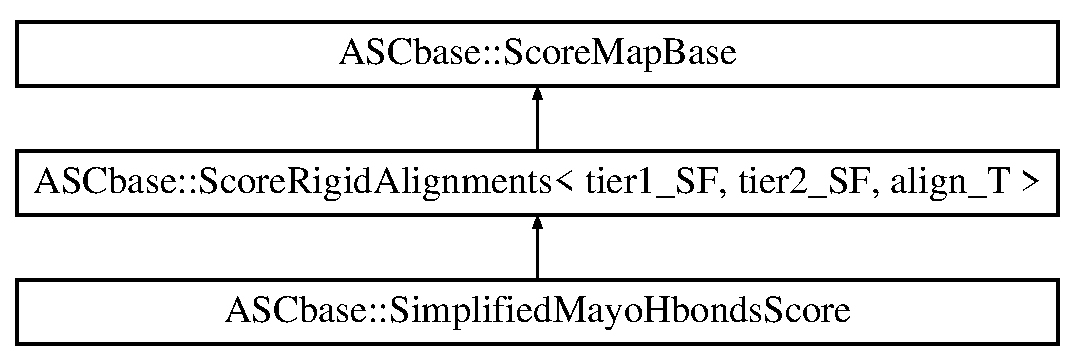
\includegraphics[height=3cm]{classASCbase_1_1SimplifiedMayoHbondsScore}
\end{center}
\end{figure}
\subsection*{Public Member Functions}
\begin{CompactItemize}
\item 
\bf{Simplified\-Mayo\-Hbonds\-Score} (\bf{Model\-Sitemap} $\ast$model\_\-in, const \bf{Search\-Parameters} \&params)
\begin{CompactList}\small\item\em Default constructor for scoring methods of rigidly aligned sitemaps. \item\end{CompactList}\item 
\bf{$\sim$Simplified\-Mayo\-Hbonds\-Score} ()\label{classASCbase_1_1SimplifiedMayoHbondsScore_079bccca92ecadc6a5dfc8752b2a71b2}

\begin{CompactList}\small\item\em basic destruction \item\end{CompactList}\end{CompactItemize}
\subsection*{Protected Member Functions}
\begin{CompactItemize}
\item 
my\_\-float\_\-t \bf{score} (const \bf{Dbase\-Sitemap} \&search, rigid\_\-align\_\-vi scores)
\begin{CompactList}\small\item\em Given an alignment of search to the query, score said alignment. \item\end{CompactList}\item 
my\_\-float\_\-t \textbf{correspondences} (my\_\-float\_\-t $\ast$$\ast$query\_\-pts\_\-ptr, my\_\-float\_\-t $\ast$$\ast$db\_\-pts\_\-ptr, size\_\-t $\ast$npts)\label{classASCbase_1_1SimplifiedMayoHbondsScore_16a1511418e1434b8a9af2a4a45771fd}

\end{CompactItemize}
\subsection*{Private Member Functions}
\begin{CompactItemize}
\item 
my\_\-float\_\-t \textbf{simp\_\-mayo\_\-fun} (hbond\_\-ideal\_\-pt\_\-vci M, hbond\_\-ideal\_\-pt\_\-vci S)\label{classASCbase_1_1SimplifiedMayoHbondsScore_98ffd12659a057084f2156f72ba62e98}

\end{CompactItemize}
\subsection*{Static Private Attributes}
\begin{CompactItemize}
\item 
static const my\_\-float\_\-t \textbf{V\_\-zero} = 8.0\label{classASCbase_1_1SimplifiedMayoHbondsScore_7fbedaf8d613548425a7927950ca6499}

\item 
static const my\_\-float\_\-t \textbf{d\_\-zero} = 2.8\label{classASCbase_1_1SimplifiedMayoHbondsScore_484beeed25a3dc66b615b45b965b4034}

\item 
static const my\_\-float\_\-t \textbf{d\_\-zero\_\-squared} = d\_\-zero$\ast$d\_\-zero\label{classASCbase_1_1SimplifiedMayoHbondsScore_ec8144f93af7dc412e9f1a8eec9871cd}

\item 
static const std::string \bf{A\_\-fname} = \char`\"{}Simplified\-Mayo\-Hbonds\-Score.C\char`\"{}\label{classASCbase_1_1SimplifiedMayoHbondsScore_f94c16b357f8c124b7dd01eb297ee0f0}

\begin{CompactList}\small\item\em Source file name. \item\end{CompactList}\end{CompactItemize}
\subsection*{Classes}
\begin{CompactItemize}
\item 
struct \textbf{S\_\-and\_\-M}
\end{CompactItemize}


\subsection{Detailed Description}
Base class for scoring rigid alignments of dbase sitemaps to a given model. 



\subsection{Constructor \& Destructor Documentation}
\index{ASCbase::SimplifiedMayoHbondsScore@{ASCbase::Simplified\-Mayo\-Hbonds\-Score}!SimplifiedMayoHbondsScore@{SimplifiedMayoHbondsScore}}
\index{SimplifiedMayoHbondsScore@{SimplifiedMayoHbondsScore}!ASCbase::SimplifiedMayoHbondsScore@{ASCbase::Simplified\-Mayo\-Hbonds\-Score}}
\subsubsection{\setlength{\rightskip}{0pt plus 5cm}Simplified\-Mayo\-Hbonds\-Score::Simplified\-Mayo\-Hbonds\-Score (\bf{Model\-Sitemap} $\ast$ {\em model\_\-in}, const \bf{Search\-Parameters} \& {\em params})}\label{classASCbase_1_1SimplifiedMayoHbondsScore_70771cd00d33a3ee88c11bbb36ae5068}


Default constructor for scoring methods of rigidly aligned sitemaps. 

\begin{Desc}
\item[Parameters:]
\begin{description}
\item[{\em model\_\-in}]Pointer to the model points (sitemap class) \item[{\em params}]Reference to the search's runtime parameters \end{description}
\end{Desc}


\subsection{Member Function Documentation}
\index{ASCbase::SimplifiedMayoHbondsScore@{ASCbase::Simplified\-Mayo\-Hbonds\-Score}!score@{score}}
\index{score@{score}!ASCbase::SimplifiedMayoHbondsScore@{ASCbase::Simplified\-Mayo\-Hbonds\-Score}}
\subsubsection{\setlength{\rightskip}{0pt plus 5cm}my\_\-float\_\-t Simplified\-Mayo\-Hbonds\-Score::score (const \bf{Dbase\-Sitemap} \& {\em search}, rigid\_\-align\_\-vi {\em scores})\hspace{0.3cm}{\tt  [protected]}}\label{classASCbase_1_1SimplifiedMayoHbondsScore_855918f5ffd04e320e9270f07878fc75}


Given an alignment of search to the query, score said alignment. 

\begin{Desc}
\item[Parameters:]
\begin{description}
\item[{\em search}]Pointer to the sitemap aligned to the model sitemap \end{description}
\end{Desc}
\begin{Desc}
\item[Returns:]The score of the alignment \end{Desc}


The documentation for this class was generated from the following files:\begin{CompactItemize}
\item 
Simplified\-Mayo\-Hbonds\-Score.H\item 
Simplified\-Mayo\-Hbonds\-Score.C\end{CompactItemize}

\section{ASCbase::Sitemap Class Reference}
\label{classASCbase_1_1Sitemap}\index{ASCbase::Sitemap@{ASCbase::Sitemap}}
{\tt \#include $<$Sitemap.H$>$}

Inheritance diagram for ASCbase::Sitemap::\begin{figure}[H]
\begin{center}
\leavevmode
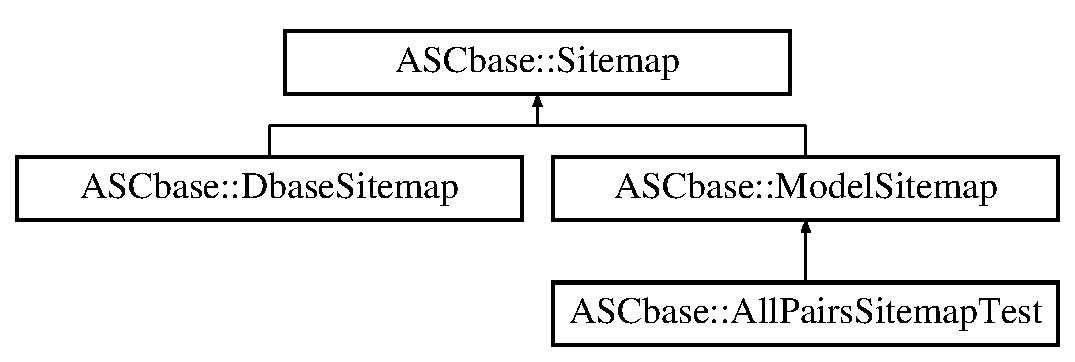
\includegraphics[height=3cm]{classASCbase_1_1Sitemap}
\end{center}
\end{figure}
\subsection*{Public Member Functions}
\begin{CompactItemize}
\item 
\bf{Sitemap} (const std::string path, const std::string struct\_\-id, const \bf{Base\-Parameters} \&args, const bool normalize=true, const bool load\_\-hbond\_\-surfaces=false, const bool hydrophobic\_\-query=false, const verbose\_\-level\_\-t verbosity=VERBOSE\_\-SILENT)\label{classASCbase_1_1Sitemap_50c5a65ec5c3b1e196466431ab71637a}

\begin{CompactList}\small\item\em Read/load a sitemap. \item\end{CompactList}\item 
\bf{Sitemap} (const \bf{Gen\-Points\-Parameters} \&usr\_\-args)\label{classASCbase_1_1Sitemap_fc5a254b492d94440c55970ef63386f2}

\begin{CompactList}\small\item\em First step in creating a sitemap. \item\end{CompactList}\item 
virtual \bf{$\sim$Sitemap} ()\label{classASCbase_1_1Sitemap_efd8a95708982d72800caf7f69073700}

\begin{CompactList}\small\item\em Typical cleanup of dynamic mem. \item\end{CompactList}\item 
bool \bf{fail} () const 
\begin{CompactList}\small\item\em Check if class is viable. \item\end{CompactList}\item 
bool \bf{write\_\-files} (const std::string struct\_\-id, const std::string path)\label{classASCbase_1_1Sitemap_88720d257d371462b7fc1b8c797aa697}

\begin{CompactList}\small\item\em Write the three sitemap files. \item\end{CompactList}\item 
bool \bf{has\_\-enough\_\-points} ()
\item 
std::string \bf{atoms\_\-file\_\-name} () const \label{classASCbase_1_1Sitemap_aaf9fd841e8f5a03b2b7b756240bbe82}

\begin{CompactList}\small\item\em Get the filename of the PDB structure used to generate the sitemap. \item\end{CompactList}\item 
std::string \bf{ligand\_\-file\_\-name} () const \label{classASCbase_1_1Sitemap_cb41876f6caf930dbfd134532ba02a0c}

\begin{CompactList}\small\item\em Get the filename of the mol2 ligand used to generate the sitemap. \item\end{CompactList}\item 
const \bf{Sitemap\-Atoms\-File} \& \textbf{interacting\_\-atoms} () const \label{classASCbase_1_1Sitemap_8cef15e389674f18b95f808397f30163}

\item 
\bf{Sitemap\-Atoms\-File} \& \textbf{interacting\_\-atoms} ()\label{classASCbase_1_1Sitemap_49015f2e7b31c7f19a0a47abc9af3db2}

\item 
const \bf{PDBStructure} \& \textbf{bind\_\-site\_\-atoms} () const \label{classASCbase_1_1Sitemap_e56f41b7103116460be52ca6be7f2549}

\item 
\bf{PDBStructure} \& \textbf{bind\_\-site\_\-atoms} ()\label{classASCbase_1_1Sitemap_7c01c7079e267cf260d1c7e255ae6b6f}

\item 
const \bf{Sitemap\-Points\-File} \& \textbf{sitemap\_\-points} () const \label{classASCbase_1_1Sitemap_5bdd019adc94558d333e1b988a574b32}

\item 
interact\_\-pts\_\-vci \textbf{interact\_\-pts\_\-beg} () const \label{classASCbase_1_1Sitemap_a7ad7e74e6ef0cdfb3e8e487e2db6200}

\item 
interact\_\-pts\_\-vci \textbf{interact\_\-pts\_\-end} () const \label{classASCbase_1_1Sitemap_fe90bda50b24ac3ecfa92df9d698b7d1}

\item 
void \textbf{transform\_\-interact\_\-pts} (my\_\-float\_\-t $\ast$R, my\_\-float\_\-t $\ast$T)\label{classASCbase_1_1Sitemap_dbd2a6cb931e9a427fa8543216600632}

\item 
void \textbf{revert\_\-interact\_\-pts} ()\label{classASCbase_1_1Sitemap_ec8a4a45362b46f0fd2f25db0876f488}

\item 
void \textbf{interact\_\-pts\_\-centroid\_\-3D} (my\_\-float\_\-t $\ast$C)\label{classASCbase_1_1Sitemap_f6ea975d404459e84b1283b3d011434f}

\item 
\bf{Hbond\-Points} \& \bf{hbond\_\-points} ()\label{classASCbase_1_1Sitemap_007b084d4422bb7a72bdd63e309985ce}

\begin{CompactList}\small\item\em Get a reference to the sitemap hbond points. \item\end{CompactList}\item 
const \bf{Hbond\-Points} \& \bf{hbond\_\-points} () const \label{classASCbase_1_1Sitemap_d985aeaf02eedb866b67eb389e62df52}

\begin{CompactList}\small\item\em Get a const reference to the sitemap hbond points. \item\end{CompactList}\item 
\bf{Hphob\-Points} \& \bf{hphob\_\-points} ()\label{classASCbase_1_1Sitemap_ac2a508a7cb5843d2450b4261de23b93}

\begin{CompactList}\small\item\em Get a reference to the sitemap hphob points. \item\end{CompactList}\item 
const \bf{Hphob\-Points} \& \bf{hphob\_\-points} () const \label{classASCbase_1_1Sitemap_0ee5530e8852f95876a978e8c284f88f}

\begin{CompactList}\small\item\em Get a const reference to the sitemap hphob points. \item\end{CompactList}\item 
size\_\-t \textbf{fit\_\-points\_\-size} () const \label{classASCbase_1_1Sitemap_88f86e7f2f8a1a69a6e34a1b6b942216}

\item 
const my\_\-float\_\-t $\ast$ \textbf{get\_\-norm\_\-moments} () const \label{classASCbase_1_1Sitemap_df498664611c91d15cf7234d8ef91dbc}

\item 
void \textbf{transform\_\-bind\_\-site\_\-res\_\-pos} (const my\_\-float\_\-t $\ast$R, const my\_\-float\_\-t $\ast$T)\label{classASCbase_1_1Sitemap_22aa833d2798ec1ecc85f29444a60dc2}

\item 
void \textbf{revert\_\-bind\_\-site\_\-res\_\-pos} ()\label{classASCbase_1_1Sitemap_2411adae66ef848c5bfe67d55c07e672}

\item 
const \bf{Bounding\-Volume} \& \textbf{bounding\_\-volume\_\-handle} () const \label{classASCbase_1_1Sitemap_3ba92f5ed263d28b96b29085c197abed}

\item 
const \bf{Bounding\-Volume} \& \textbf{site\_\-volume\_\-estimate\_\-handle} () const \label{classASCbase_1_1Sitemap_ad6269d1f92809bbf093a0c6f6c8442a}

\item 
void \textbf{revert} ()\label{classASCbase_1_1Sitemap_85a7198a79dd727691347e20c5ffffef}

\item 
my\_\-float\_\-t \bf{compute\_\-RMSD} () const 
\item 
void \bf{transform} (const my\_\-float\_\-t $\ast$R, const my\_\-float\_\-t $\ast$T)\label{classASCbase_1_1Sitemap_5dc7a050ffc9ae70c203cb31e41b4b77}

\begin{CompactList}\small\item\em Transform the objects that comprise the model of the binding site. \item\end{CompactList}\item 
void \bf{inverse\_\-transform} (const my\_\-float\_\-t $\ast$R, const my\_\-float\_\-t $\ast$T)
\item 
Hbond\-Surfaces$<$ \bf{hbond\_\-surface\_\-t} $>$ \& \textbf{hbond\_\-surfaces} () const \label{classASCbase_1_1Sitemap_9e75ff867b2874ad6365c5c67c27a941}

\item 
std::string \textbf{site\_\-path} () const \label{classASCbase_1_1Sitemap_25f76f5d2bfbce099424bce78913d77b}

\item 
std::string \textbf{get\_\-struct\_\-id} () const \label{classASCbase_1_1Sitemap_325a5ef0a4b1949fd1d7eb8622a91802}

\item 
void \bf{compute\_\-max\_\-feature\_\-values} (std::vector$<$ my\_\-float\_\-t $>$ $\ast$max\_\-feat\_\-vals) const 
\item 
my\_\-float\_\-t \bf{compute\_\-site\_\-vol\_\-intersect} (const \bf{Sitemap} \&other) const 
\end{CompactItemize}
\subsection*{Protected Member Functions}
\begin{CompactItemize}
\item 
void \textbf{set\_\-fail\_\-flag} (const bool val)\label{classASCbase_1_1Sitemap_e250f1412ec1750e343811d8582cd562}

\item 
bool \textbf{load\_\-volume} (std::string path, std::string struct\_\-id, std::string dbase\_\-sites, std::string vol\_\-tag, \bf{Bounding\-Volume} $\ast$$\ast$vol, geometry::sphere\_\-t $\ast$S=0)\label{classASCbase_1_1Sitemap_79a3b9c79bdd450b23932618525d67ae}

\end{CompactItemize}
\subsection*{Protected Attributes}
\begin{CompactItemize}
\item 
\bf{Hbond\-Points} $\ast$ \bf{hbond\_\-pts}\label{classASCbase_1_1Sitemap_dcd2dacc1cda6d35e9e477e38ab1af5b}

\begin{CompactList}\small\item\em Hydrophillic portion of sitemap. \item\end{CompactList}\item 
\bf{Hphob\-Points} $\ast$ \bf{hphob\_\-pts}\label{classASCbase_1_1Sitemap_89271f4fedad4a8435ff3f30e58bb7f7}

\begin{CompactList}\small\item\em Hydrophobic portion of sitemap. \item\end{CompactList}\item 
\bf{interact\_\-pts\_\-vec} \textbf{interact\_\-points}\label{classASCbase_1_1Sitemap_ff5f52340679a7c4c44521a8f7218324}

\item 
\bf{Bounding\-Volume} $\ast$ \bf{A\_\-site\_\-vol\_\-est}\label{classASCbase_1_1Sitemap_cb78a63c2111c987ecd011d1dd3d1ce0}

\begin{CompactList}\small\item\em Upper estimate of the site volume. \item\end{CompactList}\end{CompactItemize}
\subsection*{Private Member Functions}
\begin{CompactItemize}
\item 
void \bf{init} ()\label{classASCbase_1_1Sitemap_2c579b022413645a8ecbdc4317117563}

\begin{CompactList}\small\item\em Initialize class pointer variables to zero (NULL). \item\end{CompactList}\item 
bool \textbf{get\_\-user\_\-surf\_\-patches} (const std::string \&lig\_\-fname, const std::string \&scratch\_\-dir, const std::string \&sphere\_\-str, const std::string \&user\_\-vert\_\-fname)\label{classASCbase_1_1Sitemap_bc73bf05cc0b7795b178657d537ab7d9}

\item 
bool \textbf{get\_\-MSMS\_\-surf\_\-patches} (const std::string \&lig\_\-fname, const std::string \&scratch\_\-dir, const std::string \&sphere\_\-str, const std::string \&install\_\-dir, const bool include\_\-metals, const std::string \&msms\_\-binary, const std::vector$<$ std::string $>$ \&waters)\label{classASCbase_1_1Sitemap_a35e5cc0fa7e11df3b9f5f237a01ab5c}

\item 
bool \bf{get\_\-norm\_\-stats} (const std::string csv\_\-fname, const \bf{Base\-Parameters} \&args, bool hydrophobic\_\-query=false)\label{classASCbase_1_1Sitemap_d692fc3eae9705af5c3b5151a18aad82}

\begin{CompactList}\small\item\em Get the normalization stats for the given sitemap file. \item\end{CompactList}\item 
\bf{Bounding\-Volume} $\ast$ \bf{setup\_\-volume} (const std::string ligand\_\-fname, const my\_\-float\_\-t grid\_\-spacing, const std::string sphere\_\-str, const bool use\_\-union\_\-of\_\-balls)
\begin{CompactList}\small\item\em Setup the sitemap volume. \item\end{CompactList}\item 
void \textbf{get\_\-prot\_\-interact\_\-atoms} (const \bf{PDBStructure} $\ast$prot, \bf{Bounding\-Volume} $\ast$site\_\-vol, std::vector$<$ atom\_\-vci $>$ $\ast$bind\_\-atoms, std::vector$<$ atom\_\-vci $>$ $\ast$rad\_\-atoms, interact\_\-atoms\_\-vec $\ast$hbond\_\-atoms, interact\_\-atoms\_\-vec $\ast$hphob\_\-atoms, hphob\_\-triad\_\-vec $\ast$hphob\_\-triads, const int min\_\-chain\_\-size)\label{classASCbase_1_1Sitemap_b38affd80a93bb4445f22c732b79e8cb}

\item 
void \bf{find\_\-binding\_\-site\_\-hbonds} (const \bf{Gen\-Points\-Parameters::hbond\_\-method\_\-t} hbond\_\-density, const std::string params\_\-dir, const std::vector$<$ std::string $>$ \&waters, \bf{Bounding\-Volume} $\ast$site\_\-vol, const interact\_\-atoms\_\-vec \&hbond\_\-atoms, std::vector$<$ atom\_\-vci $>$ $\ast$bind\_\-atoms, std::vector$<$ atom\_\-vci $>$ $\ast$rad\_\-atoms)
\item 
bool \bf{find\_\-binding\_\-site\_\-metals} ()\label{classASCbase_1_1Sitemap_4fcf9aa2c2a4afcf1d21bd3038434d7d}

\begin{CompactList}\small\item\em Calculate the template points for all metal atoms in the binding site. \item\end{CompactList}\item 
bool \bf{find\_\-binding\_\-site\_\-hphobs} (const \bf{Gen\-Points\-Parameters::hphob\_\-method\_\-t} hphob\_\-method, const my\_\-float\_\-t cluster\_\-diameter, const interact\_\-atoms\_\-vec \&hphob\_\-atoms, const hphob\_\-triad\_\-vec \&hphob\_\-triads, const std::vector$<$ atom\_\-vci $>$ \&bind\_\-atoms, \bf{Bounding\-Volume} $\ast$site\_\-vol, const sphere\_\-sample\_\-level\_\-t sample\_\-level=DISCRETE\_\-SPHERE\_\-LEVEL\_\-TWO)
\item 
void \bf{write\_\-feature\_\-scales} (std::ostream \&out)\label{classASCbase_1_1Sitemap_1596bc4cf18ba4f6709a67f3e30437cb}

\begin{CompactList}\small\item\em Write out the largest value possible for each feature. \item\end{CompactList}\item 
void \textbf{clean\_\-up\_\-string} (std::string \&S)\label{classASCbase_1_1Sitemap_0894845a3e513c909d694bbd0fdcaba3}

\item 
void \textbf{build\_\-points\_\-header} (const \bf{Gen\-Points\-Parameters} \&args)\label{classASCbase_1_1Sitemap_2f3a6d65a3e920903d9d4869c168510d}

\item 
bool \textbf{gen\_\-lig\_\-box} (const std::string fname, my\_\-float\_\-t $\ast$corners)\label{classASCbase_1_1Sitemap_583a1a32407f665be875abee7e6744d2}

\item 
void \textbf{get\_\-site\_\-volume\_\-estimate} (hbond\_\-fit\_\-pt\_\-vci hbond\_\-pts\_\-beg, hbond\_\-fit\_\-pt\_\-vci hbond\_\-pts\_\-end, hphob\_\-point\_\-lci hphob\_\-points\_\-beg, hphob\_\-point\_\-lci hphob\_\-points\_\-end, size\_\-t npts, my\_\-float\_\-t vol\_\-est\_\-tol)\label{classASCbase_1_1Sitemap_6fc2cf350f7c9dbe24ef402196d601d5}

\item 
bool \textbf{load\_\-ligand} (const std::string \&fname, \bf{Coord\-File} $\ast$$\ast$lig)\label{classASCbase_1_1Sitemap_4c1be8761d14961907869cd902292581}

\item 
bool \textbf{get\_\-prot\_\-atom\_\-close\_\-to\_\-ligand} (const std::string ligand\_\-fname, std::vector$<$ atom\_\-vci $>$ \&bind\_\-atoms, atom\_\-vci $\ast$close\_\-atom)\label{classASCbase_1_1Sitemap_d896226d048c6c0f9347bee48b938f86}

\end{CompactItemize}
\subsection*{Private Attributes}
\begin{CompactItemize}
\item 
verbose\_\-level\_\-t \textbf{verbose}\label{classASCbase_1_1Sitemap_b030f50473b6d8670e571d51003f424d}

\item 
\bf{Bounding\-Volume} $\ast$ \textbf{A\_\-site\_\-vol}\label{classASCbase_1_1Sitemap_6990d012cf2b73d02b1a953df6bea5b9}

\item 
\bf{Sitemap\-Atoms\-File} $\ast$ \bf{A\_\-site\_\-atoms}\label{classASCbase_1_1Sitemap_aacf141914798bdd7861687e432628f8}

\begin{CompactList}\small\item\em Atoms from residues near the binding site. \item\end{CompactList}\item 
\bf{PDBStructure} $\ast$ \textbf{A\_\-bind\_\-site\_\-res}\label{classASCbase_1_1Sitemap_2a52e689037b97d6a36e93507c7883ea}

\item 
\bf{Sitemap\-Points\-File} $\ast$ \textbf{points}\label{classASCbase_1_1Sitemap_0d487acfbafbcd354984bc9ee12d4f18}

\item 
\bf{PDBStructure} $\ast$ \textbf{prot\_\-atoms}\label{classASCbase_1_1Sitemap_d14802c86d41cb3aebbad567ab57cde0}

\item 
atom\_\-map\_\-t \textbf{interact\_\-atoms}\label{classASCbase_1_1Sitemap_104c9c8b0dc2d1c8239e24ff9ae16d30}

\item 
my\_\-float\_\-t \textbf{A\_\-norm\_\-moments} [2]\label{classASCbase_1_1Sitemap_3b31d195203a3e0b86a9b4e42f29aefe}

\item 
my\_\-float\_\-t \textbf{A\_\-hphob\_\-norm\_\-moments} [2]\label{classASCbase_1_1Sitemap_710b85700b6359566aa94d1cb3b23ad0}

\item 
Hbond\-Surfaces$<$ \bf{hbond\_\-surface\_\-t} $>$ $\ast$ \textbf{A\_\-hbond\_\-surfaces}\label{classASCbase_1_1Sitemap_746f37a116532d40ebfb917405f79f56}

\item 
\bf{Simple\-Trimesh} $\ast$ \textbf{old\_\-binding\_\-site\_\-mesh}\label{classASCbase_1_1Sitemap_67d0c9dd4ca44665912f7927effd2478}

\item 
geometry::sphere\_\-t \bf{A\_\-site\_\-vol\_\-est\_\-as\_\-sphere}\label{classASCbase_1_1Sitemap_d868aaadd592ee46383e0ab2e9cc9350}

\begin{CompactList}\small\item\em I don't have the time to compute the intersection of the different bounding volume classes -- use this instead. \item\end{CompactList}\item 
std::string \bf{A\_\-site\_\-path}\label{classASCbase_1_1Sitemap_f9703909778c885c912a1415910f988f}

\begin{CompactList}\small\item\em Directory holding the sitemap. \item\end{CompactList}\item 
std::string \bf{A\_\-struct\_\-id}\label{classASCbase_1_1Sitemap_1355b26f18d6bd22405fc2ed95543b68}

\begin{CompactList}\small\item\em Structure ID of the site map. \item\end{CompactList}\item 
std::string \bf{A\_\-dbase\_\-ligs}\label{classASCbase_1_1Sitemap_f759f963ef40e2d5b8bfe0805f70e2f8}

\begin{CompactList}\small\item\em Directory holding dbase ligands. \item\end{CompactList}\item 
std::string \bf{A\_\-lig\_\-fname}\label{classASCbase_1_1Sitemap_8687cc1a0a4f3c900d40bc3b3ba7b4bb}

\begin{CompactList}\small\item\em Name of the ligand file. \item\end{CompactList}\item 
std::string \bf{A\_\-atoms\_\-fname}\label{classASCbase_1_1Sitemap_22af7b3e2f83f482711f96fd2b8036fb}

\begin{CompactList}\small\item\em Name of the sitemap atoms file. \item\end{CompactList}\item 
bool \textbf{A\_\-include\_\-metals}\label{classASCbase_1_1Sitemap_085592f9e6ab4a46b1717d17e15f3590}

\item 
bool \textbf{A\_\-MSMS\_\-surf}\label{classASCbase_1_1Sitemap_cc87543764821d5965c02426e3b621c0}

\item 
bool \textbf{A\_\-user\_\-surf}\label{classASCbase_1_1Sitemap_8a9754cb39062045c87758860244e132}

\item 
my\_\-float\_\-t \bf{A\_\-probe\_\-radius}\label{classASCbase_1_1Sitemap_7474a2670e5f74e20594a2add689f8d5}

\begin{CompactList}\small\item\em Probe radius for MSMS. \item\end{CompactList}\item 
my\_\-float\_\-t \bf{A\_\-num\_\-pts\_\-per\_\-area}\label{classASCbase_1_1Sitemap_f9dbc37200a6d1841ea366760f8d0837}

\begin{CompactList}\small\item\em Number of points per (A)$^\wedge$2. \item\end{CompactList}\item 
int \textbf{A\_\-min\_\-res\_\-per\_\-chain}\label{classASCbase_1_1Sitemap_ca99b08072b44f7f26cd714417333b44}

\item 
bool \textbf{A\_\-fail}\label{classASCbase_1_1Sitemap_960c9c48a78c77be9eae68071e34e987}

\end{CompactItemize}
\subsection*{Static Private Attributes}
\begin{CompactItemize}
\item 
static const int \textbf{MIN\_\-NUMBER\_\-POINTS\_\-\_\-POLAR\_\-SITE} = 20\label{classASCbase_1_1Sitemap_693e69f1d3787c869c7510692bcd0e91}

\item 
static const int \textbf{MIN\_\-NUMBER\_\-POINTS\_\-\_\-HPHOB\_\-SITE} = 30\label{classASCbase_1_1Sitemap_fd1fc07d472e969eb867e04bbe1170e6}

\item 
static const my\_\-float\_\-t \textbf{TOLERANCE} = 2.0\label{classASCbase_1_1Sitemap_872ebaa52aa3fdf3501804dd35077f84}

\item 
static const my\_\-float\_\-t \bf{MAXRADDIST}\label{classASCbase_1_1Sitemap_5eeb7fdc83ae79798995a668a58b42e1}

\begin{CompactList}\small\item\em Max rad file dist? \item\end{CompactList}\item 
static const my\_\-float\_\-t \bf{MAXBINDDIST}\label{classASCbase_1_1Sitemap_7cf5dd107e339908dc8ca026eba23360}

\begin{CompactList}\small\item\em Max interaction with binding site dist. \item\end{CompactList}\item 
static const std::string \bf{A\_\-fname} = \char`\"{}Sitemap.C\char`\"{}\label{classASCbase_1_1Sitemap_b28ac13500885c7b52d35446d3fa89de}

\begin{CompactList}\small\item\em Name of source file. \item\end{CompactList}\end{CompactItemize}


\subsection{Detailed Description}
Both generates and loads sitemaps. Kinda glues together the different parts in an ad hoc manner. This works, but the interface is quite clunky. 



\subsection{Member Function Documentation}
\index{ASCbase::Sitemap@{ASCbase::Sitemap}!compute_max_feature_values@{compute\_\-max\_\-feature\_\-values}}
\index{compute_max_feature_values@{compute\_\-max\_\-feature\_\-values}!ASCbase::Sitemap@{ASCbase::Sitemap}}
\subsubsection{\setlength{\rightskip}{0pt plus 5cm}void Sitemap::compute\_\-max\_\-feature\_\-values (std::vector$<$ my\_\-float\_\-t $>$ $\ast$ {\em max\_\-feat\_\-vals}) const}\label{classASCbase_1_1Sitemap_2fc4a9ede3730c0cd6fdadc97f00864b}


Compute the maximum value for each feature and store in the given vector \index{ASCbase::Sitemap@{ASCbase::Sitemap}!compute_RMSD@{compute\_\-RMSD}}
\index{compute_RMSD@{compute\_\-RMSD}!ASCbase::Sitemap@{ASCbase::Sitemap}}
\subsubsection{\setlength{\rightskip}{0pt plus 5cm}my\_\-float\_\-t ASCbase::Sitemap::compute\_\-RMSD () const\hspace{0.3cm}{\tt  [inline]}}\label{classASCbase_1_1Sitemap_81fe70b16f0e030e8c20923fc2e66a49}


Compute the root mean squared deviation (RMSD) between the current and orignial positions of the hydrogen bonding and hydrophobic points \index{ASCbase::Sitemap@{ASCbase::Sitemap}!compute_site_vol_intersect@{compute\_\-site\_\-vol\_\-intersect}}
\index{compute_site_vol_intersect@{compute\_\-site\_\-vol\_\-intersect}!ASCbase::Sitemap@{ASCbase::Sitemap}}
\subsubsection{\setlength{\rightskip}{0pt plus 5cm}my\_\-float\_\-t Sitemap::compute\_\-site\_\-vol\_\-intersect (const \bf{Sitemap} \& {\em other}) const}\label{classASCbase_1_1Sitemap_8865b700374d55d3e7b4d6c4cd489f60}


Compute the fraction of the volume of this site's volume estimate that is inside the other site's volume estimate \index{ASCbase::Sitemap@{ASCbase::Sitemap}!fail@{fail}}
\index{fail@{fail}!ASCbase::Sitemap@{ASCbase::Sitemap}}
\subsubsection{\setlength{\rightskip}{0pt plus 5cm}bool ASCbase::Sitemap::fail () const\hspace{0.3cm}{\tt  [inline]}}\label{classASCbase_1_1Sitemap_1a15e9045f766ba8e80f6411513de6ac}


Check if class is viable. 

\begin{Desc}
\item[Returns:]False if no fatal errors have occured, else true \end{Desc}
\index{ASCbase::Sitemap@{ASCbase::Sitemap}!find_binding_site_hbonds@{find\_\-binding\_\-site\_\-hbonds}}
\index{find_binding_site_hbonds@{find\_\-binding\_\-site\_\-hbonds}!ASCbase::Sitemap@{ASCbase::Sitemap}}
\subsubsection{\setlength{\rightskip}{0pt plus 5cm}void Sitemap::find\_\-binding\_\-site\_\-hbonds (const \bf{Gen\-Points\-Parameters::hbond\_\-method\_\-t} {\em hbond\_\-density}, const std::string {\em params\_\-dir}, const std::vector$<$ std::string $>$ \& {\em waters}, \bf{Bounding\-Volume} $\ast$ {\em site\_\-vol}, const interact\_\-atoms\_\-vec \& {\em hbond\_\-atoms}, std::vector$<$ atom\_\-vci $>$ $\ast$ {\em bind\_\-atoms}, std::vector$<$ atom\_\-vci $>$ $\ast$ {\em rad\_\-atoms})\hspace{0.3cm}{\tt  [private]}}\label{classASCbase_1_1Sitemap_1c89cc76612ae6e252b459b4bf62bc13}


\begin{Desc}
\item[Parameters:]
\begin{description}
\item[{\em hbond\_\-density}]Density to discretely sample hydrogen bonding volume \item[{\em params\_\-dir}]Directory holding the hbond point sampling files \item[{\em site\_\-vol}]Pointer to the sitemap volume \item[{\em include\_\-waters}]True implies include all water molecules in the protein structure as \char`\"{}part of the protein\char`\"{}. \item[{\em include\_\-metals}]True implies include all metal atoms in the the protein structure as \char`\"{}part of the protein\char`\"{}. \item[{\em rad\_\-atoms}]Pointer to vector to hold rad atoms. \end{description}
\end{Desc}
\index{ASCbase::Sitemap@{ASCbase::Sitemap}!find_binding_site_hphobs@{find\_\-binding\_\-site\_\-hphobs}}
\index{find_binding_site_hphobs@{find\_\-binding\_\-site\_\-hphobs}!ASCbase::Sitemap@{ASCbase::Sitemap}}
\subsubsection{\setlength{\rightskip}{0pt plus 5cm}bool Sitemap::find\_\-binding\_\-site\_\-hphobs (const \bf{Gen\-Points\-Parameters::hphob\_\-method\_\-t} {\em hphob\_\-method}, const my\_\-float\_\-t {\em cluster\_\-diameter}, const interact\_\-atoms\_\-vec \& {\em hphob\_\-atoms}, const hphob\_\-triad\_\-vec \& {\em hphob\_\-triads}, const std::vector$<$ atom\_\-vci $>$ \& {\em bind\_\-atoms}, \bf{Bounding\-Volume} $\ast$ {\em site\_\-vol}, const sphere\_\-sample\_\-level\_\-t {\em sample\_\-level} = {\tt DISCRETE\_\-SPHERE\_\-LEVEL\_\-TWO})\hspace{0.3cm}{\tt  [private]}}\label{classASCbase_1_1Sitemap_955ee3f2bcb9a0853c49c98f9664310b}


\begin{Desc}
\item[Parameters:]
\begin{description}
\item[{\em hphob\_\-method}]which hydrophobic model/method to use \item[{\em cluster\_\-diameter}]The maximum cluster diameter for complete link clustering of hphob points. \item[{\em rad\_\-atoms}]Reference to the rad atoms (returned from hbonds method) \end{description}
\end{Desc}
\begin{Desc}
\item[Returns:]!fail() \end{Desc}
\index{ASCbase::Sitemap@{ASCbase::Sitemap}!has_enough_points@{has\_\-enough\_\-points}}
\index{has_enough_points@{has\_\-enough\_\-points}!ASCbase::Sitemap@{ASCbase::Sitemap}}
\subsubsection{\setlength{\rightskip}{0pt plus 5cm}bool Sitemap::has\_\-enough\_\-points ()}\label{classASCbase_1_1Sitemap_e9d2433452ba04908e7ef43cbe7d8c3c}


Determine if the site map has enough points given the current implementation of the site maps, alignment method, and alignment techniques scoring \index{ASCbase::Sitemap@{ASCbase::Sitemap}!inverse_transform@{inverse\_\-transform}}
\index{inverse_transform@{inverse\_\-transform}!ASCbase::Sitemap@{ASCbase::Sitemap}}
\subsubsection{\setlength{\rightskip}{0pt plus 5cm}void ASCbase::Sitemap::inverse\_\-transform (const my\_\-float\_\-t $\ast$ {\em R}, const my\_\-float\_\-t $\ast$ {\em T})\hspace{0.3cm}{\tt  [inline]}}\label{classASCbase_1_1Sitemap_9923d897faab8e6b015908311241ac3a}


Transform the objects that comprise the model of the binding site using the inverse of the transform defined by R \& T \index{ASCbase::Sitemap@{ASCbase::Sitemap}!setup_volume@{setup\_\-volume}}
\index{setup_volume@{setup\_\-volume}!ASCbase::Sitemap@{ASCbase::Sitemap}}
\subsubsection{\setlength{\rightskip}{0pt plus 5cm}\bf{Bounding\-Volume} $\ast$ Sitemap::setup\_\-volume (const std::string {\em ligand\_\-fname}, const my\_\-float\_\-t {\em grid\_\-spacing}, const std::string {\em sphere\_\-str}, const bool {\em use\_\-union\_\-of\_\-balls})\hspace{0.3cm}{\tt  [private]}}\label{classASCbase_1_1Sitemap_dbc5be7e837523050ebf38da9fca1d1f}


Setup the sitemap volume. 

\begin{Desc}
\item[Parameters:]
\begin{description}
\item[{\em ligand\_\-fname}]Path to the ligand to define the binding site volume \item[{\em grid\_\-spacing}]The rectuangular grid sampling distance \item[{\em sphere\_\-str}]Sphere as center and radius in a string \item[{\em use\_\-union\_\-of\_\-balls}]If a ligand is given and use\_\-union\_\-of\_\-balls is true, take the union of balls (1 centered at each ligand atom) as the volume estimate and not the ligand bounding box. \end{description}
\end{Desc}
\begin{Desc}
\item[Returns:]Pointer to the volume object or NULL if an error occured \end{Desc}


The documentation for this class was generated from the following files:\begin{CompactItemize}
\item 
Sitemap.H\item 
Sitemap.C\end{CompactItemize}

\section{ASCbase::sitemap\_\-variables\_\-t Struct Reference}
\label{structASCbase_1_1sitemap__variables__t}\index{ASCbase::sitemap_variables_t@{ASCbase::sitemap\_\-variables\_\-t}}
Container for args from command line, parameter files and env variables.  


{\tt \#include $<$Sitemap\-Defs.H$>$}

\subsection*{Public Attributes}
\begin{CompactItemize}
\item 
char $\ast$ \bf{pts\_\-fname}\label{structASCbase_1_1sitemap__variables__t_85023c58ca8199341e073b66de1309ff}

\begin{CompactList}\small\item\em File name to store the sitemap. \item\end{CompactList}\item 
char $\ast$ \bf{protein\_\-fname}\label{structASCbase_1_1sitemap__variables__t_08d611868163121dfa6083f2265f2b9a}

\begin{CompactList}\small\item\em Protein file to use to generate the sitemap. \item\end{CompactList}\item 
char $\ast$ \bf{ligand\_\-fname}\label{structASCbase_1_1sitemap__variables__t_b192da1b9c611409dda2762f266f2f8d}

\begin{CompactList}\small\item\em Ligand file to use to define sitemap volume. \item\end{CompactList}\item 
char $\ast$ \bf{ligs\_\-dir}\label{structASCbase_1_1sitemap__variables__t_9209d76febae9ba180b5da6ad237e402}

\begin{CompactList}\small\item\em Default ligands directory. \item\end{CompactList}\item 
char $\ast$ \bf{proteins\_\-dir}\label{structASCbase_1_1sitemap__variables__t_079ccca327e81108ffa7b5ebda75b72b}

\begin{CompactList}\small\item\em Default proteins directory. \item\end{CompactList}\item 
char $\ast$ \bf{work\_\-dir}\label{structASCbase_1_1sitemap__variables__t_b4c8e92a25e8659139365e489cf7d5d3}

\begin{CompactList}\small\item\em Scratch directory. \item\end{CompactList}\item 
char $\ast$ \bf{hbond\_\-dens\_\-str}\label{structASCbase_1_1sitemap__variables__t_8d23a8f0fece77b6720972a9ccb38771}

\begin{CompactList}\small\item\em string of the desired hbond density \item\end{CompactList}\item 
char $\ast$ \bf{sphere\_\-str}\label{structASCbase_1_1sitemap__variables__t_9d1d9d528f2e67c292a79eb12d343f2b}

\begin{CompactList}\small\item\em string of the center and radius sphere \item\end{CompactList}\item 
my\_\-float\_\-t \bf{cluster\_\-diameter}\label{structASCbase_1_1sitemap__variables__t_e2234821022ddc0b1bfd001fbc29d035}

\begin{CompactList}\small\item\em Maximal cluster diameter for complete link. \item\end{CompactList}\item 
my\_\-float\_\-t \bf{grid\_\-spacing}\label{structASCbase_1_1sitemap__variables__t_90d5f33a206ea3f421bba55e2e72601b}

\begin{CompactList}\small\item\em The length of a side of a grid cube. \item\end{CompactList}\item 
hbond\_\-method\_\-t \bf{hbond\_\-method}\label{structASCbase_1_1sitemap__variables__t_8569b43e6c79f7a203cf8c6f47bf34c6}

\begin{CompactList}\small\item\em Denotes how densely to represent hbonds. \item\end{CompactList}\item 
hphob\_\-method\_\-t \bf{hphob\_\-method}\label{structASCbase_1_1sitemap__variables__t_2a80a7d61e4e7b4062d4f7add6a5fb06}

\begin{CompactList}\small\item\em Denotes which hueristical method to use. \item\end{CompactList}\item 
sphere\_\-sample\_\-level\_\-t \textbf{sphere\_\-sample\_\-level}\label{structASCbase_1_1sitemap__variables__t_a45236ac5b594ec4cefad791b4f152b1}

\item 
int \textbf{sphere\_\-sample\_\-level\_\-int}\label{structASCbase_1_1sitemap__variables__t_d2fb2b8ce3b46216370b6006d8e757aa}

\item 
bool \bf{normalize}\label{structASCbase_1_1sitemap__variables__t_74cbcaa59bfae447d25c367ca3eab643}

\begin{CompactList}\small\item\em True implies get mean and variance for sitemap. \item\end{CompactList}\item 
verbose\_\-level\_\-t \bf{verbose}\label{structASCbase_1_1sitemap__variables__t_f9d61423254f0b0be183097564d60d2f}

\begin{CompactList}\small\item\em How much to write to stdout. \item\end{CompactList}\end{CompactItemize}


\subsection{Detailed Description}
Container for args from command line, parameter files and env variables. 



The documentation for this struct was generated from the following file:\begin{CompactItemize}
\item 
Sitemap\-Defs.H\end{CompactItemize}

\section{ASCbase::Sitemap\-Atoms\-File Class Reference}
\label{classASCbase_1_1SitemapAtomsFile}\index{ASCbase::SitemapAtomsFile@{ASCbase::SitemapAtomsFile}}
The structure atoms which gave rise to the sitemap (interaction) points.  


{\tt \#include $<$Sitemap\-Atoms\-File.H$>$}

Inheritance diagram for ASCbase::Sitemap\-Atoms\-File::\begin{figure}[H]
\begin{center}
\leavevmode
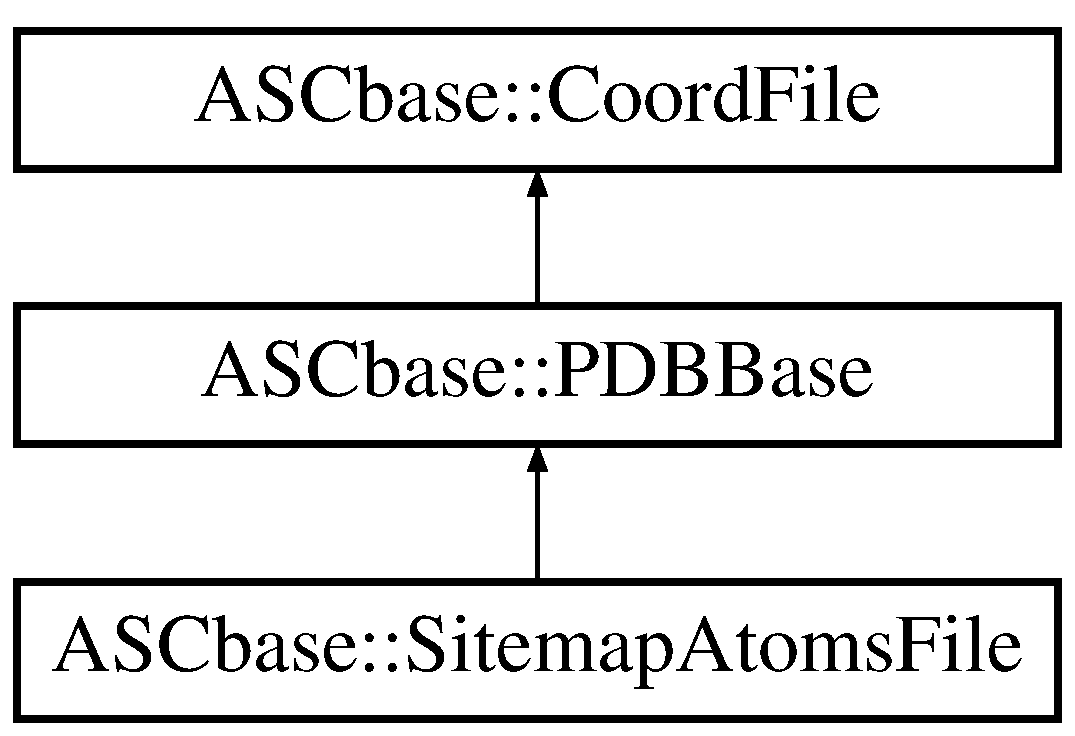
\includegraphics[height=3cm]{classASCbase_1_1SitemapAtomsFile}
\end{center}
\end{figure}
\subsection*{Public Member Functions}
\begin{CompactItemize}
\item 
\bf{Sitemap\-Atoms\-File} (const std::string filename, const verbose\_\-level\_\-t verbosity=VERBOSE\_\-SILENT)
\begin{CompactList}\small\item\em Load a sitemap atoms file. \item\end{CompactList}\item 
\bf{Sitemap\-Atoms\-File} (const atom\_\-map\_\-t \&a\_\-tbl)
\begin{CompactList}\small\item\em Populate the atoms by appending all the atoms in the input table (map). \item\end{CompactList}\item 
\bf{Sitemap\-Atoms\-File} (\bf{PDBStructure} $\ast$prot\_\-atoms, const atom\_\-map\_\-t \&a\_\-tbl, const std::string lig\_\-fname, const int min\_\-chain\_\-size, const my\_\-float\_\-t max\_\-interact\_\-dist=\bf{A\_\-max\_\-interact\_\-dist})
\item 
\bf{Sitemap\-Atoms\-File} (\bf{PDBStructure} $\ast$prot\_\-atoms, \bf{Bounding\-Volume} $\ast$site\_\-vol, const int min\_\-chain\_\-size, const atom\_\-map\_\-t \&a\_\-tbl)
\item 
\bf{$\sim$Sitemap\-Atoms\-File} ()\label{classASCbase_1_1SitemapAtomsFile_a27d46f9dd14aceb62fdae18eda326a2}

\begin{CompactList}\small\item\em Do nothing dstr. \item\end{CompactList}\item 
void \bf{write\_\-xyzr} (std::ostream \&out, const atom\_\-vci close\_\-atom, uint $\ast$close\_\-atom\_\-idx)
\begin{CompactList}\small\item\em Write all the non-hydrogen atoms to 'out' in xyzr format. \item\end{CompactList}\end{CompactItemize}
\subsection*{Static Private Attributes}
\begin{CompactItemize}
\item 
static const my\_\-float\_\-t \bf{A\_\-max\_\-interact\_\-dist} = 12.0\label{classASCbase_1_1SitemapAtomsFile_f3f59c7e4edce05a17cdb09291ca7899}

\begin{CompactList}\small\item\em maximum prot-lig atom interaction distance \item\end{CompactList}\item 
static const std::string \bf{A\_\-fname} = \char`\"{}Sitemap\-Atoms\-File.C\char`\"{}\label{classASCbase_1_1SitemapAtomsFile_dcffcac9c78d0b3d352b120ecc218a95}

\begin{CompactList}\small\item\em Name of source file. \item\end{CompactList}\end{CompactItemize}


\subsection{Detailed Description}
The structure atoms which gave rise to the sitemap (interaction) points. 



\subsection{Constructor \& Destructor Documentation}
\index{ASCbase::SitemapAtomsFile@{ASCbase::Sitemap\-Atoms\-File}!SitemapAtomsFile@{SitemapAtomsFile}}
\index{SitemapAtomsFile@{SitemapAtomsFile}!ASCbase::SitemapAtomsFile@{ASCbase::Sitemap\-Atoms\-File}}
\subsubsection{\setlength{\rightskip}{0pt plus 5cm}Sitemap\-Atoms\-File::Sitemap\-Atoms\-File (const std::string {\em filename}, const verbose\_\-level\_\-t {\em verbosity} = {\tt VERBOSE\_\-SILENT})}\label{classASCbase_1_1SitemapAtomsFile_0b8a59ad5194d59da0f6e8116f85cf3f}


Load a sitemap atoms file. 

Load the sitemap atoms file given the path stored in filename

\begin{Desc}
\item[Parameters:]
\begin{description}
\item[{\em filename}]Path to the sitemap atoms file to load \item[{\em verbosity}]If is REPORT, send something to stdout \end{description}
\end{Desc}
\index{ASCbase::SitemapAtomsFile@{ASCbase::Sitemap\-Atoms\-File}!SitemapAtomsFile@{SitemapAtomsFile}}
\index{SitemapAtomsFile@{SitemapAtomsFile}!ASCbase::SitemapAtomsFile@{ASCbase::Sitemap\-Atoms\-File}}
\subsubsection{\setlength{\rightskip}{0pt plus 5cm}Sitemap\-Atoms\-File::Sitemap\-Atoms\-File (const atom\_\-map\_\-t \& {\em a\_\-tbl})}\label{classASCbase_1_1SitemapAtomsFile_03b65bb9aacf200908c1f432e68b7861}


Populate the atoms by appending all the atoms in the input table (map). 

\begin{Desc}
\item[Parameters:]
\begin{description}
\item[{\em a\_\-tbl}]Reference to a table (map) holding atoms keyed by atom number (PDB serial) \end{description}
\end{Desc}
\index{ASCbase::SitemapAtomsFile@{ASCbase::Sitemap\-Atoms\-File}!SitemapAtomsFile@{SitemapAtomsFile}}
\index{SitemapAtomsFile@{SitemapAtomsFile}!ASCbase::SitemapAtomsFile@{ASCbase::Sitemap\-Atoms\-File}}
\subsubsection{\setlength{\rightskip}{0pt plus 5cm}Sitemap\-Atoms\-File::Sitemap\-Atoms\-File (\bf{PDBStructure} $\ast$ {\em prot\_\-atoms}, const atom\_\-map\_\-t \& {\em a\_\-tbl}, const std::string {\em lig\_\-fname}, const int {\em min\_\-chain\_\-size}, const my\_\-float\_\-t {\em max\_\-interact\_\-dist} = {\tt \bf{A\_\-max\_\-interact\_\-dist}})}\label{classASCbase_1_1SitemapAtomsFile_66a28af4029b17cf26ee549ed8a4e0c4}


Populate the atoms by appending all residues which have at least one atom within interaction distance of any ligand atom \index{ASCbase::SitemapAtomsFile@{ASCbase::Sitemap\-Atoms\-File}!SitemapAtomsFile@{SitemapAtomsFile}}
\index{SitemapAtomsFile@{SitemapAtomsFile}!ASCbase::SitemapAtomsFile@{ASCbase::Sitemap\-Atoms\-File}}
\subsubsection{\setlength{\rightskip}{0pt plus 5cm}Sitemap\-Atoms\-File::Sitemap\-Atoms\-File (\bf{PDBStructure} $\ast$ {\em prot\_\-atoms}, \bf{Bounding\-Volume} $\ast$ {\em site\_\-vol}, const int {\em min\_\-chain\_\-size}, const atom\_\-map\_\-t \& {\em a\_\-tbl})}\label{classASCbase_1_1SitemapAtomsFile_a91864e8664d1f11b0734dba8de1f7d7}


Populate the atoms by appending all residues which have at least one atom within the \char`\"{}original\char`\"{} bounding volume plus an additional buffer of max\_\-interaction\_\-dist 

\subsection{Member Function Documentation}
\index{ASCbase::SitemapAtomsFile@{ASCbase::Sitemap\-Atoms\-File}!write_xyzr@{write\_\-xyzr}}
\index{write_xyzr@{write\_\-xyzr}!ASCbase::SitemapAtomsFile@{ASCbase::Sitemap\-Atoms\-File}}
\subsubsection{\setlength{\rightskip}{0pt plus 5cm}void Sitemap\-Atoms\-File::write\_\-xyzr (std::ostream \& {\em out}, const atom\_\-vci {\em close\_\-atom}, uint $\ast$ {\em close\_\-atom\_\-idx})}\label{classASCbase_1_1SitemapAtomsFile_309e10428c0eb0eaef737a0c4b1773e8}


Write all the non-hydrogen atoms to 'out' in xyzr format. 

Note: if one want certain types of atoms, etc, they should be specified through the constructor interface or possibly use \doxyref{PDBStructure}{p.}{classASCbase_1_1PDBStructure} instead 

The documentation for this class was generated from the following files:\begin{CompactItemize}
\item 
Sitemap\-Atoms\-File.H\item 
Sitemap\-Atoms\-File.C\end{CompactItemize}

\section{ASCbase::Sitemap\-Points\-File Class Reference}
\label{classASCbase_1_1SitemapPointsFile}\index{ASCbase::SitemapPointsFile@{ASCbase::SitemapPointsFile}}
Creation and storage of sitemap points files.  


{\tt \#include $<$Sitemap\-Points\-File.H$>$}

Inheritance diagram for ASCbase::Sitemap\-Points\-File::\begin{figure}[H]
\begin{center}
\leavevmode
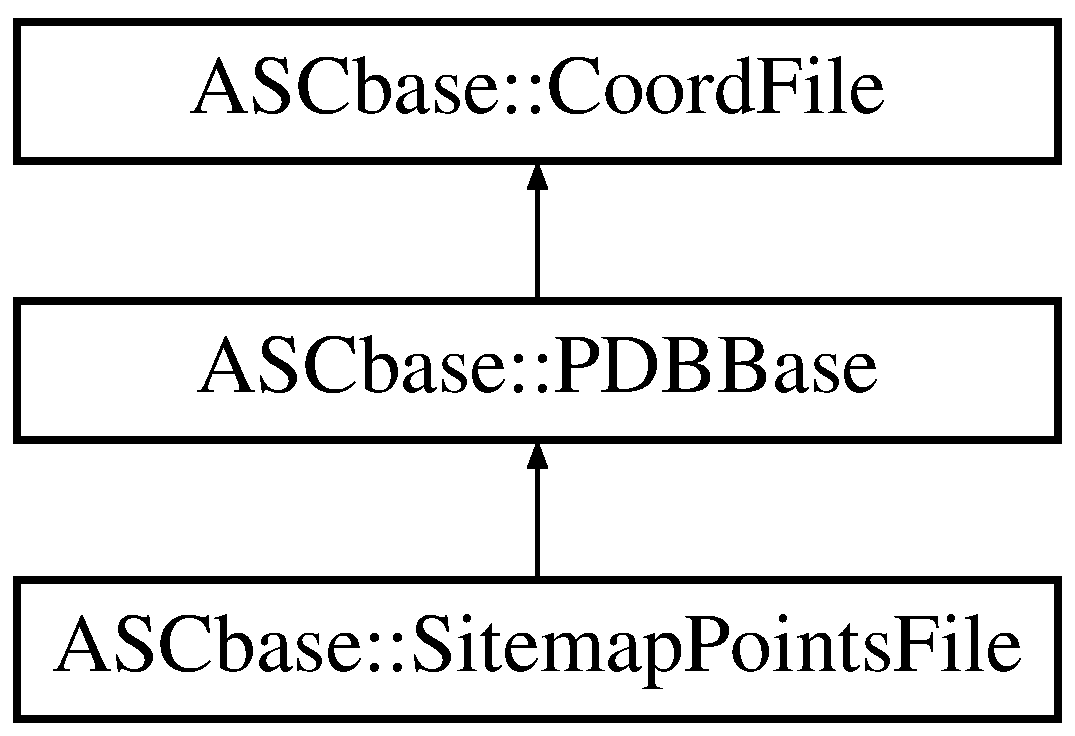
\includegraphics[height=3cm]{classASCbase_1_1SitemapPointsFile}
\end{center}
\end{figure}
\subsection*{Public Member Functions}
\begin{CompactItemize}
\item 
\bf{Sitemap\-Points\-File} ()\label{classASCbase_1_1SitemapPointsFile_db5b966cb4e3f26a969479259b7a63b5}

\begin{CompactList}\small\item\em Cstr to create a sitemap points file. \item\end{CompactList}\item 
\bf{Sitemap\-Points\-File} (const std::string filename, const verbose\_\-level\_\-t verbosity=VERBOSE\_\-SILENT)\label{classASCbase_1_1SitemapPointsFile_5f355b3286eaea41596b433e8d5cd476}

\begin{CompactList}\small\item\em Cstr to load an existing sitemap points file. \item\end{CompactList}\item 
bool \bf{add\_\-points} (const hbond\_\-fit\_\-pt\_\-vci \_\-begin, const hbond\_\-fit\_\-pt\_\-vci \_\-end)\label{classASCbase_1_1SitemapPointsFile_0f7b8e2ccb3f1dc27fcc4720b0ae14c5}

\begin{CompactList}\small\item\em Add hydrogen bonding points. \item\end{CompactList}\item 
bool \bf{add\_\-points} (const hphob\_\-point\_\-lci \_\-begin, const hphob\_\-point\_\-lci \_\-end)\label{classASCbase_1_1SitemapPointsFile_5dd5cd935f9623f2e8e3ce4051c156ba}

\begin{CompactList}\small\item\em Add hydrophobic points. \item\end{CompactList}\item 
const uint \textbf{num\_\-polar\_\-points} () const \label{classASCbase_1_1SitemapPointsFile_4a9728a68610afe41d65332ff73bcbf2}

\item 
const uint \textbf{num\_\-hphobic\_\-points} () const \label{classASCbase_1_1SitemapPointsFile_5d261bb85ca34bf9797ab126d8c46960}

\end{CompactItemize}
\subsection*{Private Attributes}
\begin{CompactItemize}
\item 
std::vector$<$ uint $>$ \bf{counts}\label{classASCbase_1_1SitemapPointsFile_b3c2f62fc9252fb70d4287d889c7b9fa}

\begin{CompactList}\small\item\em Shamelessly assumes header comes before data. \item\end{CompactList}\end{CompactItemize}
\subsection*{Static Private Attributes}
\begin{CompactItemize}
\item 
static const std::string \bf{\_\-fname} = \char`\"{}Sitemap\-Points\-File.C\char`\"{}\label{classASCbase_1_1SitemapPointsFile_3c2df5c3e3de9995d61644c28d181c42}

\begin{CompactList}\small\item\em Source file name. \item\end{CompactList}\end{CompactItemize}


\subsection{Detailed Description}
Creation and storage of sitemap points files. 



The documentation for this class was generated from the following files:\begin{CompactItemize}
\item 
Sitemap\-Points\-File.H\item 
Sitemap\-Points\-File.C\end{CompactItemize}

\section{ASCbase::Sites\-Score\-Base Class Reference}
\label{classASCbase_1_1SitesScoreBase}\index{ASCbase::SitesScoreBase@{ASCbase::SitesScoreBase}}
Base class for scoring two (aligned) sites.  


{\tt \#include $<$Sites\-Score\-Base.H$>$}

Inheritance diagram for ASCbase::Sites\-Score\-Base::\begin{figure}[H]
\begin{center}
\leavevmode
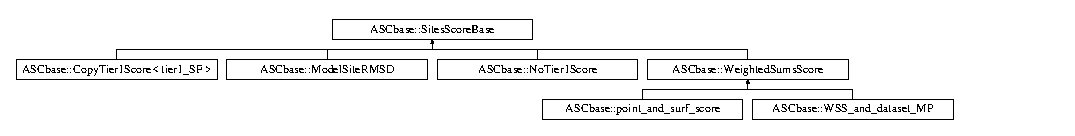
\includegraphics[height=1.37705cm]{classASCbase_1_1SitesScoreBase}
\end{center}
\end{figure}
\subsection*{Public Types}
\begin{CompactItemize}
\item 
typedef std::less$<$ my\_\-float\_\-t $>$ \textbf{score\_\-cmp}\label{classASCbase_1_1SitesScoreBase_00e957c70676d80311e1dbd5e1c0125c}

\item 
typedef std::vector$<$ Model\-Hbond\-Surfaces::m\_\-surf\_\-vci $>$::const\_\-iterator \bf{m\_\-cap\_\-iters\_\-vci}\label{classASCbase_1_1SitesScoreBase_9d9b97ecd62e491da147bcd90a9b5ea2}

\begin{CompactList}\small\item\em A lower score is more favorable -- change this in derived class to std::greater if a higher score is more favorable. \item\end{CompactList}\end{CompactItemize}
\subsection*{Public Member Functions}
\begin{CompactItemize}
\item 
\bf{Sites\-Score\-Base} ()\label{classASCbase_1_1SitesScoreBase_fe6fe8c907ded1c532a5d4c6a39455ae}

\begin{CompactList}\small\item\em Default constructor for site map point scoring of (aligned) sitemaps. \item\end{CompactList}\item 
virtual \bf{$\sim$Sites\-Score\-Base} ()\label{classASCbase_1_1SitesScoreBase_e4c453e87a899eda609ae5273c90304d}

\begin{CompactList}\small\item\em basic destruction \item\end{CompactList}\item 
virtual my\_\-float\_\-t \bf{score} (const \bf{Model\-Sitemap} \&model, const \bf{Dbase\-Sitemap} \&dbase, \bf{rigid\_\-align\_\-t} $\ast$scores)=0
\item 
virtual my\_\-float\_\-t \bf{correspondences} (const \bf{Model\-Sitemap} \&model, my\_\-float\_\-t $\ast$$\ast$query\_\-pts\_\-ptr, my\_\-float\_\-t $\ast$$\ast$db\_\-pts\_\-ptr, size\_\-t $\ast$npts)\label{classASCbase_1_1SitesScoreBase_81a209231e8da6c4cd2c67e904960c23}

\begin{CompactList}\small\item\em Get the latest correspondences of the db to query sites. \item\end{CompactList}\item 
virtual my\_\-float\_\-t \bf{polar\_\-correspondences} (const \bf{Model\-Sitemap} \&model, my\_\-float\_\-t $\ast$$\ast$vertices\_\-ptr, my\_\-float\_\-t $\ast$$\ast$closest\_\-pts\_\-ptr, size\_\-t $\ast$npts) const \label{classASCbase_1_1SitesScoreBase_058e354d1bc501409ad71f2eb15d49aa}

\begin{CompactList}\small\item\em Used for ICP where we want the correspondences in an array. \item\end{CompactList}\item 
virtual void \bf{polar\_\-correspondences} (const \bf{Model\-Sitemap} \&model, \bf{m\_\-cap\_\-iters\_\-vci} cap\_\-iters\_\-beg, \bf{m\_\-cap\_\-iters\_\-vci} cap\_\-iters\_\-end, std::vector$<$ const my\_\-float\_\-t $\ast$ $>$ $\ast$q\_\-pts, std::vector$<$ const my\_\-float\_\-t $\ast$ $>$ $\ast$corr\_\-pts) const \label{classASCbase_1_1SitesScoreBase_ef470380314023e120d6a784ceb20cf2}

\begin{CompactList}\small\item\em Used for IK where not all of the caps may be mobile. \item\end{CompactList}\item 
virtual void \textbf{correspondences} (const \bf{Model\-Sitemap} \&model, std::vector$<$ const my\_\-float\_\-t $\ast$ $>$ $\ast$q\_\-pts, std::vector$<$ const my\_\-float\_\-t $\ast$ $>$ $\ast$corr\_\-pts)\label{classASCbase_1_1SitesScoreBase_e7f8ada741da2d1704504d889d2b19a6}

\item 
virtual bool \bf{uses\_\-surface\_\-mesh} ()
\item 
virtual bool \bf{uses\_\-hbond\_\-surfaces} ()
\item 
void \bf{set\_\-scale\_\-terms} (bool scale\_\-in)\label{classASCbase_1_1SitesScoreBase_a1056836ee286cbc66e8e957651845d4}

\begin{CompactList}\small\item\em Set the class variable scale\_\-terms to the given value. \item\end{CompactList}\item 
const bool \bf{scale\_\-terms} () const 
\item 
virtual const bool \bf{score\_\-is\_\-noop} () const 
\begin{CompactList}\small\item\em Is the function score a no op? \item\end{CompactList}\end{CompactItemize}
\subsection*{Private Attributes}
\begin{CompactItemize}
\item 
bool \textbf{A\_\-scale\_\-terms}\label{classASCbase_1_1SitesScoreBase_d2221aec98270cd955290c5c27936800}

\end{CompactItemize}


\subsection{Detailed Description}
Base class for scoring two (aligned) sites. 

This class defines the interface required for a class to be able to be used to score two sites. A derived class can be used at either level of the scoring (template parameter 1 or 2 of \doxyref{Score\-Rigid\-Alignments}{p.}{classASCbase_1_1ScoreRigidAlignments})

notes on template parameters: align\_\-T: must be \doxyref{rigid\_\-align\_\-t}{p.}{classASCbase_1_1rigid__align__t} or derived class 



\subsection{Member Function Documentation}
\index{ASCbase::SitesScoreBase@{ASCbase::Sites\-Score\-Base}!scale_terms@{scale\_\-terms}}
\index{scale_terms@{scale\_\-terms}!ASCbase::SitesScoreBase@{ASCbase::Sites\-Score\-Base}}
\subsubsection{\setlength{\rightskip}{0pt plus 5cm}const bool ASCbase::Sites\-Score\-Base::scale\_\-terms () const\hspace{0.3cm}{\tt  [inline]}}\label{classASCbase_1_1SitesScoreBase_ed5a9dc6b14b13e8bb94cbdd4e3bd8ed}


Should each term be linearly scaled to from [0.0, max] to [0.0, 1.0] where max is the maximum value the query site can have for that term? \index{ASCbase::SitesScoreBase@{ASCbase::Sites\-Score\-Base}!score@{score}}
\index{score@{score}!ASCbase::SitesScoreBase@{ASCbase::Sites\-Score\-Base}}
\subsubsection{\setlength{\rightskip}{0pt plus 5cm}virtual my\_\-float\_\-t ASCbase::Sites\-Score\-Base::score (const \bf{Model\-Sitemap} \& {\em model}, const \bf{Dbase\-Sitemap} \& {\em dbase}, \bf{rigid\_\-align\_\-t} $\ast$ {\em scores})\hspace{0.3cm}{\tt  [pure virtual]}}\label{classASCbase_1_1SitesScoreBase_651f05f08e15b7ea8f7fa7c41973499e}


\begin{Desc}
\item[Parameters:]
\begin{description}
\item[{\em model}]Const ref to the model site \item[{\em dbase}]Const ref to the sitemap aligned to the model sitemap \item[{\em scores}]iterator to the score data class \item[{\em save\_\-correspondences}]should the score method save the points correspondences? Saving is required for methods like ICP \end{description}
\end{Desc}
\begin{Desc}
\item[Returns:]The score of the alignment \end{Desc}


Implemented in \bf{ASCbase::Model\-Site\-RMSD} \doxyref{p.}{classASCbase_1_1ModelSiteRMSD_3eb593c527ae195f94705cbc6b3ff335}, \bf{ASCbase::No\-Tier1Score} \doxyref{p.}{classASCbase_1_1NoTier1Score_1d4f4670c8831e655105788395100367}, \bf{ASCbase::point\_\-and\_\-surf\_\-score} \doxyref{p.}{classASCbase_1_1point__and__surf__score_f7086e180c849bba8a8a1df984a3b114}, and \bf{ASCbase::Weighted\-Sums\-Score} \doxyref{p.}{classASCbase_1_1WeightedSumsScore_eeee8c834449ce75686bb076f40c3ee4}.\index{ASCbase::SitesScoreBase@{ASCbase::Sites\-Score\-Base}!score_is_noop@{score\_\-is\_\-noop}}
\index{score_is_noop@{score\_\-is\_\-noop}!ASCbase::SitesScoreBase@{ASCbase::Sites\-Score\-Base}}
\subsubsection{\setlength{\rightskip}{0pt plus 5cm}virtual const bool ASCbase::Sites\-Score\-Base::score\_\-is\_\-noop () const\hspace{0.3cm}{\tt  [inline, virtual]}}\label{classASCbase_1_1SitesScoreBase_3db1e7181ba314fa327df0bbbd1ba458}


Is the function score a no op? 

It is safe to return false here since, this class is a pure virtual class 

Reimplemented in \bf{ASCbase::No\-Tier1Score} \doxyref{p.}{classASCbase_1_1NoTier1Score_63778c92095132cf82e34d7d5d62f7f8}.\index{ASCbase::SitesScoreBase@{ASCbase::Sites\-Score\-Base}!uses_hbond_surfaces@{uses\_\-hbond\_\-surfaces}}
\index{uses_hbond_surfaces@{uses\_\-hbond\_\-surfaces}!ASCbase::SitesScoreBase@{ASCbase::Sites\-Score\-Base}}
\subsubsection{\setlength{\rightskip}{0pt plus 5cm}virtual bool ASCbase::Sites\-Score\-Base::uses\_\-hbond\_\-surfaces ()\hspace{0.3cm}{\tt  [inline, virtual]}}\label{classASCbase_1_1SitesScoreBase_a7a5fcc3e24663874f8066c00089f3cf}


Derived class should return false, unless the derived class is using the hydrogen bond surface caps 

Reimplemented in \bf{ASCbase::Copy\-Tier1Score$<$ tier1\_\-SF $>$} \doxyref{p.}{classASCbase_1_1CopyTier1Score_79790bb098d9f4d8c49951458c155534}, \bf{ASCbase::Model\-Site\-RMSD} \doxyref{p.}{classASCbase_1_1ModelSiteRMSD_8eb481fde2008dc2d6e60a3a4679bb07}, \bf{ASCbase::No\-Tier1Score} \doxyref{p.}{classASCbase_1_1NoTier1Score_173cc857bbcd62849e9462cfa8c78a4b}, \bf{ASCbase::point\_\-and\_\-surf\_\-score} \doxyref{p.}{classASCbase_1_1point__and__surf__score_8f006a0249c062673acec07465b4d686}, and \bf{ASCbase::Weighted\-Sums\-Score} \doxyref{p.}{classASCbase_1_1WeightedSumsScore_a54a5a22b71dd4bc14aaf06f7756eca7}.\index{ASCbase::SitesScoreBase@{ASCbase::Sites\-Score\-Base}!uses_surface_mesh@{uses\_\-surface\_\-mesh}}
\index{uses_surface_mesh@{uses\_\-surface\_\-mesh}!ASCbase::SitesScoreBase@{ASCbase::Sites\-Score\-Base}}
\subsubsection{\setlength{\rightskip}{0pt plus 5cm}virtual bool ASCbase::Sites\-Score\-Base::uses\_\-surface\_\-mesh ()\hspace{0.3cm}{\tt  [inline, virtual]}}\label{classASCbase_1_1SitesScoreBase_ae4a2a1ae9113bcad0535593c210030f}


Derived class should return false, unless, the site's surface needs to be to be rotated and translated 

Reimplemented in \bf{ASCbase::Copy\-Tier1Score$<$ tier1\_\-SF $>$} \doxyref{p.}{classASCbase_1_1CopyTier1Score_507e5fdffb914519b624cf87b7470479}, \bf{ASCbase::Model\-Site\-RMSD} \doxyref{p.}{classASCbase_1_1ModelSiteRMSD_f0f87f1b1293e8c294d24922ba2458b3}, \bf{ASCbase::No\-Tier1Score} \doxyref{p.}{classASCbase_1_1NoTier1Score_39452ebad1db68af8cc2e3a4cb08953e}, \bf{ASCbase::point\_\-and\_\-surf\_\-score} \doxyref{p.}{classASCbase_1_1point__and__surf__score_92345073d3e38666cb95cca9adc14ae3}, and \bf{ASCbase::Weighted\-Sums\-Score} \doxyref{p.}{classASCbase_1_1WeightedSumsScore_9d12b648a5adc7dff9d6058d6239a314}.

The documentation for this class was generated from the following file:\begin{CompactItemize}
\item 
Sites\-Score\-Base.H\end{CompactItemize}

\section{ASCbase::Surf\-Deps\-Joints Class Reference}
\label{classASCbase_1_1SurfDepsJoints}\index{ASCbase::SurfDepsJoints@{ASCbase::SurfDepsJoints}}
Atoms (joints) and surface vertices that depend on rotatable joints.  


{\tt \#include $<$Surf\-Deps\-Joints.H$>$}

\subsection*{Public Types}
\begin{CompactItemize}
\item 
typedef std::map$<$ residue\_\-vci, \bf{pos\_\-dep\_\-on\_\-joints} $>$ \textbf{res\_\-to\_\-verts\_\-map}\label{classASCbase_1_1SurfDepsJoints_316ae96b9db4556ce0244c88f41d680c}

\item 
typedef res\_\-to\_\-verts\_\-map::iterator \textbf{res\_\-to\_\-verts\_\-mi}\label{classASCbase_1_1SurfDepsJoints_e26b5fed19a3641ad008bfc55772a463}

\item 
typedef res\_\-to\_\-verts\_\-map::const\_\-iterator \textbf{res\_\-to\_\-verts\_\-mci}\label{classASCbase_1_1SurfDepsJoints_f1373f13b08b0cb8aca30efb548dc1a6}

\item 
\textbf{JACOBIAN}\label{classASCbase_1_1SurfDepsJoints_560742b76595dd55fccd15bf18b40e607761d353bf420f282da81c11995598a8}

\item 
\textbf{PINV\_\-JACOBIAN}\label{classASCbase_1_1SurfDepsJoints_560742b76595dd55fccd15bf18b40e60ebfdcae202539532cc482f2ef9a9a969}

\item 
enum \textbf{mat\_\-type} \{ \textbf{JACOBIAN}, 
\textbf{PINV\_\-JACOBIAN}
 \}
\end{CompactItemize}
\subsection*{Public Member Functions}
\begin{CompactItemize}
\item 
\textbf{Surf\-Deps\-Joints} (\bf{prot\_\-joint\_\-dep} \&joints, \bf{PDBStructure} $\ast$prot, geometry::Transformable\-Trimesh $\ast$surf, Model\-Hbond\-Surfaces $\ast$hbond\_\-surfaces, \bf{Hbond\-Points} $\ast$hbond\_\-pts)\label{classASCbase_1_1SurfDepsJoints_5680f50b97eca320f525ae90985747a3}

\item 
void \bf{compute\_\-dihedrals\_\-and\_\-verts\_\-J} ()\label{classASCbase_1_1SurfDepsJoints_139426fae21dbc20a3a6a3c7dbf8c54c}

\begin{CompactList}\small\item\em Jacobian that give dependence of joint angles on small motions of vertices. \item\end{CompactList}\item 
void \textbf{compute\_\-JJtranspose} ()\label{classASCbase_1_1SurfDepsJoints_298d0fc1edb2ddc1efcdd1f2b36f3443}

\item 
void \textbf{update\_\-positions} (const my\_\-float\_\-t $\ast$delta\_\-q)\label{classASCbase_1_1SurfDepsJoints_dfc64104fc3c39a3aff447e134e12cda}

\item 
void \textbf{compute\_\-pinv\-J\_\-transpose} ()\label{classASCbase_1_1SurfDepsJoints_30880bb61a44aecad9d100c59fbe115d}

\item 
void \textbf{write\_\-point\_\-correspondences} (std::ostream \&out) const \label{classASCbase_1_1SurfDepsJoints_8c2e24181fcea5568c6ffbd1857ae43a}

\item 
void \bf{compute\_\-dihedral\_\-angles} (std::vector$<$ std::vector$<$ my\_\-float\_\-t $>$ $>$ $\ast$angles) const \label{classASCbase_1_1SurfDepsJoints_bc4a01295624d2f5bcad3ec57773df94}

\begin{CompactList}\small\item\em Compute the dihedral angles for those sidechains that are not fixed. \item\end{CompactList}\item 
void \bf{apply\_\-verts\_\-pinv\-J\_\-to\_\-grad} (const my\_\-float\_\-t $\ast$grad\_\-F, my\_\-float\_\-t $\ast$Q)
\begin{CompactList}\small\item\em Wrapper to compute\_\-portion\_\-pinv\-Jtrans\_\-times\_\-grad for vertices. \item\end{CompactList}\item 
void \bf{apply\_\-hbond\_\-pts\_\-pinv\-J\_\-to\_\-grad} (const my\_\-float\_\-t $\ast$grad\_\-F, my\_\-float\_\-t $\ast$Q)
\begin{CompactList}\small\item\em Wrapper to compute\_\-portion\_\-pinv\-Jtrans\_\-times\_\-grad for hbond cap pts. \item\end{CompactList}\item 
void \bf{apply\_\-atoms\_\-pinv\-J\_\-to\_\-grad} (const my\_\-float\_\-t $\ast$grad\_\-F, my\_\-float\_\-t $\ast$Q, const std::vector$<$ bool $>$ \&overlap\_\-vec)\label{classASCbase_1_1SurfDepsJoints_140826a670991bf10bcd607446b279ff}

\begin{CompactList}\small\item\em Averaging method to handle overlapping atoms. \item\end{CompactList}\item 
const int \bf{nrows\_\-J} () const \label{classASCbase_1_1SurfDepsJoints_36b6e55f8699306d664f21a252a5ba56}

\begin{CompactList}\small\item\em Get the number of rows in the Jacobian. \item\end{CompactList}\item 
const int \bf{ncols\_\-J} () const \label{classASCbase_1_1SurfDepsJoints_504ff6d5d3a85c29b7991cb632ddc5f5}

\begin{CompactList}\small\item\em Get the number of columns in the Jacobian. \item\end{CompactList}\item 
const int \bf{num\_\-atom\_\-cols\_\-J} () const \label{classASCbase_1_1SurfDepsJoints_dee28e63c09450b55c560d03571f2bdd}

\begin{CompactList}\small\item\em Get the number of atom columns in the Jacobian. \item\end{CompactList}\item 
const int \bf{num\_\-vert\_\-cols\_\-J} () const \label{classASCbase_1_1SurfDepsJoints_49f30238fa55e02769664cd40711d808}

\begin{CompactList}\small\item\em Get the number of vertex columns in the Jacobian. \item\end{CompactList}\item 
const int \bf{num\_\-hbond\_\-pts\_\-cols\_\-J} () const \label{classASCbase_1_1SurfDepsJoints_141fb2d323750c0095da41cfbe229a00}

\begin{CompactList}\small\item\em Get the number of hbond pts columns in the Jacobian. \item\end{CompactList}\item 
res\_\-to\_\-verts\_\-mci \textbf{atoms\_\-dep\_\-on\_\-joints\_\-begin} () const \label{classASCbase_1_1SurfDepsJoints_3ef79398935691313fbeaf244312799e}

\item 
res\_\-to\_\-verts\_\-mci \textbf{atoms\_\-dep\_\-on\_\-joints\_\-end} () const \label{classASCbase_1_1SurfDepsJoints_d0c0a6c1b4ac65bbf3aab788d3443d49}

\item 
std::vector$<$ int $>$::const\_\-iterator \textbf{vertex\_\-idz\_\-begin} () const \label{classASCbase_1_1SurfDepsJoints_768e2bb28761a73d0e1bd777d9007f37}

\item 
std::vector$<$ int $>$::const\_\-iterator \textbf{vertex\_\-idz\_\-end} () const \label{classASCbase_1_1SurfDepsJoints_8ce7887064ca371dc9a38398ba5c0a81}

\item 
void \textbf{write\_\-mat} (std::ostream \&out, const mat\_\-type type) const \label{classASCbase_1_1SurfDepsJoints_037d0b3d26dc9faef4aab88016b1d6db}

\item 
bool \textbf{fail} () const \label{classASCbase_1_1SurfDepsJoints_327c4e4641287aca3ad12d74e586a7ed}

\item 
std::vector$<$ Model\-Hbond\-Surfaces::m\_\-surf\_\-vci $>$::const\_\-iterator \textbf{mobile\_\-cap\_\-iters\_\-begin} () const \label{classASCbase_1_1SurfDepsJoints_cb9132967ed681f304a3aa5483305525}

\item 
std::vector$<$ Model\-Hbond\-Surfaces::m\_\-surf\_\-vci $>$::const\_\-iterator \textbf{mobile\_\-cap\_\-iters\_\-end} () const \label{classASCbase_1_1SurfDepsJoints_9136b5ac1ff71cdde78a89ab6e5558b4}

\item 
void \textbf{stop\_\-rotation\_\-given\_\-atoms} (const std::vector$<$ bool $>$ \&overlap\_\-vec, std::vector$<$ bool $>$ $\ast$fix\_\-Q)\label{classASCbase_1_1SurfDepsJoints_964260669ca7efa6820247126758b3a9}

\item 
my\_\-float\_\-t \bf{site\_\-atomic\_\-rmsd} (const \bf{PDBStructure} \&dset\_\-prot) const 
\begin{CompactList}\small\item\em Compute the atomic rmsd for the query and dataset residues. \item\end{CompactList}\end{CompactItemize}
\subsection*{Private Member Functions}
\begin{CompactItemize}
\item 
void \bf{add\_\-mol\_\-surf\_\-vertices} (geometry::Transformable\-Trimesh $\ast$surf, \bf{PDBStructure} $\ast$prot)
\item 
void \bf{add\_\-hbond\_\-points} (Model\-Hbond\-Surfaces $\ast$hbond\_\-surfaces, \bf{Hbond\-Points} $\ast$hbond\_\-pts, const \bf{PDBStructure} $\ast$prot)
\begin{CompactList}\small\item\em Add the points for the hbond groups in the binding site. \item\end{CompactList}\item 
bool \bf{check\_\-containers} ()\label{classASCbase_1_1SurfDepsJoints_2e5ac87512513806b5415aa008c6a41e}

\begin{CompactList}\small\item\em Check the 3 containers to make sure they have the same residues. \item\end{CompactList}\item 
void \bf{add\_\-dependent\_\-atoms} (const \bf{PDBStructure} $\ast$prot, residue\_\-vci res)\label{classASCbase_1_1SurfDepsJoints_ab55d5b90278e690ae8607c945a41162}

\begin{CompactList}\small\item\em Add the mobile atoms for those residues that can move. \item\end{CompactList}\item 
bool \bf{determine\_\-pt\_\-dependence} (my\_\-float\_\-t $\ast$pt, const \bf{PDBStructure} $\ast$prot, residue\_\-vci res, atom\_\-vci closest\_\-atom)\label{classASCbase_1_1SurfDepsJoints_7782e94d2a21055c6ea8c528e97daee3}

\begin{CompactList}\small\item\em Add dependencies for each surface patch vertex. \item\end{CompactList}\item 
bool \bf{determine\_\-hbond\_\-dep} (Hbond\-Surfaces$<$ \bf{model\_\-hbond\_\-surf\_\-t} $>$::surfaces\_\-vci cap, const \bf{PDBStructure} $\ast$prot, residue\_\-vci $\ast$res\_\-out)\label{classASCbase_1_1SurfDepsJoints_db588d6797a5dbee35e55722429574cb}

\begin{CompactList}\small\item\em Add joint dependencies for the given hbond cap. \item\end{CompactList}\item 
bool \bf{determine\_\-hbond\_\-dep} (hbond\_\-ideal\_\-pt\_\-vci ideal\_\-pt, const \bf{PDBStructure} $\ast$prot, residue\_\-vci $\ast$res\_\-out)
\item 
void \bf{compute\_\-portion\_\-of\_\-J} (res\_\-to\_\-verts\_\-mi pts\_\-begin, res\_\-to\_\-verts\_\-mi pts\_\-end)
\item 
void \bf{compute\_\-portion\_\-of\_\-JJtranspose} (res\_\-to\_\-verts\_\-mi pts\_\-begin, res\_\-to\_\-verts\_\-mi pts\_\-end, my\_\-float\_\-t $\ast$JJtrans)\label{classASCbase_1_1SurfDepsJoints_da88391361dff24fca61364a859cf83a}

\begin{CompactList}\small\item\em Compute the Jacobian times its transpose for the given iterators. \item\end{CompactList}\item 
void \textbf{compute\_\-portion\_\-of\_\-pinv\-Jtranspose} (res\_\-to\_\-verts\_\-mi pts\_\-begin, res\_\-to\_\-verts\_\-mi pts\_\-end, my\_\-float\_\-t $\ast$JJtrans\_\-inv)\label{classASCbase_1_1SurfDepsJoints_eced98b340d0308407ec47a3601f3130}

\item 
void \bf{compute\_\-portion\_\-pinv\-Jtrans\_\-times\_\-grad} (res\_\-to\_\-verts\_\-mi pts\_\-begin, res\_\-to\_\-verts\_\-mi pts\_\-end, const my\_\-float\_\-t $\ast$grad\_\-F, my\_\-float\_\-t $\ast$Q)
\item 
void \textbf{write\_\-mat\_\-component} (res\_\-to\_\-verts\_\-mci pts\_\-begin, res\_\-to\_\-verts\_\-mci pts\_\-end, const mat\_\-type type, const std::string name, std::ostream \&out) const \label{classASCbase_1_1SurfDepsJoints_95487bc867c1cb6f6fd003b7c8040d8c}

\item 
void \bf{rotate\_\-points} (\bf{pos\_\-dep\_\-on\_\-joints} $\ast$points, const my\_\-float\_\-t $\ast$R, const my\_\-float\_\-t $\ast$joint\_\-center, const int joint\_\-number)\label{classASCbase_1_1SurfDepsJoints_1d51091baf7a06109b2b1129aa74ef51}

\begin{CompactList}\small\item\em Rotate the dependent points using R about the axis of the joint. \item\end{CompactList}\item 
void \bf{init} ()\label{classASCbase_1_1SurfDepsJoints_4cdd546f6c403da0f5417c993a8d780b}

\begin{CompactList}\small\item\em Initialize class variables. \item\end{CompactList}\end{CompactItemize}
\subsection*{Private Attributes}
\begin{CompactItemize}
\item 
bool \textbf{A\_\-have\_\-surf}\label{classASCbase_1_1SurfDepsJoints_3515dd1581f443f45dd4809d0ac47935}

\item 
bool \textbf{A\_\-have\_\-hbond\_\-surfs}\label{classASCbase_1_1SurfDepsJoints_459da037b1829e110ac910bcfe0e9dbc}

\item 
bool \textbf{A\_\-fail}\label{classASCbase_1_1SurfDepsJoints_8e1af1869bbb14062be507b84e4bdc6f}

\item 
\bf{prot\_\-joint\_\-dep} \& \textbf{A\_\-joints}\label{classASCbase_1_1SurfDepsJoints_3e32f0537b15aed5ccea9e14243a8890}

\item 
std::vector$<$ int $>$ \textbf{A\_\-vert\_\-idz}\label{classASCbase_1_1SurfDepsJoints_75401efca3702db87fda5af198caf69e}

\item 
std::map$<$ residue\_\-vci, \bf{pos\_\-dep\_\-on\_\-joints} $>$ \bf{A\_\-verts\_\-dep\_\-on\_\-joints}\label{classASCbase_1_1SurfDepsJoints_933c101738644962a378fb8cbf6293fe}

\begin{CompactList}\small\item\em Mobile molecular surface vertices. \item\end{CompactList}\item 
std::map$<$ residue\_\-vci, \bf{pos\_\-dep\_\-on\_\-joints} $>$ \bf{A\_\-atoms\_\-dep\_\-on\_\-joints}\label{classASCbase_1_1SurfDepsJoints_1505598190c319911892331ea8938359}

\begin{CompactList}\small\item\em Mobile protein atoms. \item\end{CompactList}\item 
std::map$<$ residue\_\-vci, \bf{pos\_\-dep\_\-on\_\-joints} $>$ \bf{A\_\-hbond\_\-pts\_\-dep\_\-on\_\-joints}\label{classASCbase_1_1SurfDepsJoints_f73da4e07548a3bc9c43ac05a22c5c45}

\begin{CompactList}\small\item\em Mobile hydrogen bond points (either from \doxyref{Hbond\-Points}{p.}{classASCbase_1_1HbondPoints} or Hbond\-Surfaces). \item\end{CompactList}\item 
std::vector$<$ Model\-Hbond\-Surfaces::m\_\-surf\_\-vci $>$ \textbf{A\_\-mobile\_\-caps}\label{classASCbase_1_1SurfDepsJoints_ee798f376187502fce17ae15c1530a90}

\item 
std::map$<$ residue\_\-vci, bool $>$ \bf{A\_\-site\_\-residues}\label{classASCbase_1_1SurfDepsJoints_55c02394f1ff0c70089c654aecbaf204}

\begin{CompactList}\small\item\em Used in testing Art\-Surf binding site atomic RMSD. \item\end{CompactList}\item 
int \bf{A\_\-J\_\-nrows}\label{classASCbase_1_1SurfDepsJoints_a766d13c11a97f98c38185459a05fde4}

\begin{CompactList}\small\item\em Number of rows in the full Jacobian. \item\end{CompactList}\item 
int \textbf{A\_\-J\_\-ncols}\label{classASCbase_1_1SurfDepsJoints_5c97058a99a82e417d13702ac1c6ea11}

\item 
int \textbf{A\_\-J\_\-cols\_\-in\_\-blocks} [3]\label{classASCbase_1_1SurfDepsJoints_485965d3c8d1774c9ec19326376350b2}

\item 
my\_\-float\_\-t $\ast$ \bf{A\_\-JJtranspose}\label{classASCbase_1_1SurfDepsJoints_08fbd7f761c675819074b12cebc2546b}

\begin{CompactList}\small\item\em Work space variable -- do not use ouside of class. \item\end{CompactList}\end{CompactItemize}


\subsection{Detailed Description}
Atoms (joints) and surface vertices that depend on rotatable joints. 



\subsection{Member Function Documentation}
\index{ASCbase::SurfDepsJoints@{ASCbase::Surf\-Deps\-Joints}!add_hbond_points@{add\_\-hbond\_\-points}}
\index{add_hbond_points@{add\_\-hbond\_\-points}!ASCbase::SurfDepsJoints@{ASCbase::Surf\-Deps\-Joints}}
\subsubsection{\setlength{\rightskip}{0pt plus 5cm}void Surf\-Deps\-Joints::add\_\-hbond\_\-points (Model\-Hbond\-Surfaces $\ast$ {\em hbond\_\-surfaces}, \bf{Hbond\-Points} $\ast$ {\em hbond\_\-pts}, const \bf{PDBStructure} $\ast$ {\em prot})\hspace{0.3cm}{\tt  [private]}}\label{classASCbase_1_1SurfDepsJoints_64cae8b3b33bc5f0720b2fd0ece30b92}


Add the points for the hbond groups in the binding site. 

If hbond\_\-surfaces is not null, use the given hbond\_\-surfaces, otherwise use the hbond points.

NOTE: hbond\_\-surfaces will be used to move side chains, hbond\_\-pts are NOT used to move sidechains but will \char`\"{}go along for the ride\char`\"{} if hbond\_\-surfaces are not used. \index{ASCbase::SurfDepsJoints@{ASCbase::Surf\-Deps\-Joints}!add_mol_surf_vertices@{add\_\-mol\_\-surf\_\-vertices}}
\index{add_mol_surf_vertices@{add\_\-mol\_\-surf\_\-vertices}!ASCbase::SurfDepsJoints@{ASCbase::Surf\-Deps\-Joints}}
\subsubsection{\setlength{\rightskip}{0pt plus 5cm}void Surf\-Deps\-Joints::add\_\-mol\_\-surf\_\-vertices (geometry::Transformable\-Trimesh $\ast$ {\em surf}, \bf{PDBStructure} $\ast$ {\em prot})\hspace{0.3cm}{\tt  [private]}}\label{classASCbase_1_1SurfDepsJoints_6486c83e3b26177a18146ff3c02fd99e}


Add the vertices for the given molecular surface to the points that can move \index{ASCbase::SurfDepsJoints@{ASCbase::Surf\-Deps\-Joints}!apply_hbond_pts_pinvJ_to_grad@{apply\_\-hbond\_\-pts\_\-pinvJ\_\-to\_\-grad}}
\index{apply_hbond_pts_pinvJ_to_grad@{apply\_\-hbond\_\-pts\_\-pinvJ\_\-to\_\-grad}!ASCbase::SurfDepsJoints@{ASCbase::Surf\-Deps\-Joints}}
\subsubsection{\setlength{\rightskip}{0pt plus 5cm}void ASCbase::Surf\-Deps\-Joints::apply\_\-hbond\_\-pts\_\-pinv\-J\_\-to\_\-grad (const my\_\-float\_\-t $\ast$ {\em grad\_\-F}, my\_\-float\_\-t $\ast$ {\em Q})\hspace{0.3cm}{\tt  [inline]}}\label{classASCbase_1_1SurfDepsJoints_a7f58f0be3da964c49b2cbfbceff3fe9}


Wrapper to compute\_\-portion\_\-pinv\-Jtrans\_\-times\_\-grad for hbond cap pts. 

Assumptions: len(grad\_\-F) $>$= 3$\ast$(A\_\-J\_\-cols\_\-in\_\-blocks[1]) len(Q) $>$= A\_\-J\_\-nrows \index{ASCbase::SurfDepsJoints@{ASCbase::Surf\-Deps\-Joints}!apply_verts_pinvJ_to_grad@{apply\_\-verts\_\-pinvJ\_\-to\_\-grad}}
\index{apply_verts_pinvJ_to_grad@{apply\_\-verts\_\-pinvJ\_\-to\_\-grad}!ASCbase::SurfDepsJoints@{ASCbase::Surf\-Deps\-Joints}}
\subsubsection{\setlength{\rightskip}{0pt plus 5cm}void ASCbase::Surf\-Deps\-Joints::apply\_\-verts\_\-pinv\-J\_\-to\_\-grad (const my\_\-float\_\-t $\ast$ {\em grad\_\-F}, my\_\-float\_\-t $\ast$ {\em Q})\hspace{0.3cm}{\tt  [inline]}}\label{classASCbase_1_1SurfDepsJoints_ce7a325c8a075b2b7e22e35dfea71fb0}


Wrapper to compute\_\-portion\_\-pinv\-Jtrans\_\-times\_\-grad for vertices. 

Assumptions: len(grad\_\-F) $>$= 3$\ast$(A\_\-J\_\-cols\_\-in\_\-blocks[0]) len(Q) $>$= A\_\-J\_\-nrows \index{ASCbase::SurfDepsJoints@{ASCbase::Surf\-Deps\-Joints}!compute_portion_of_J@{compute\_\-portion\_\-of\_\-J}}
\index{compute_portion_of_J@{compute\_\-portion\_\-of\_\-J}!ASCbase::SurfDepsJoints@{ASCbase::Surf\-Deps\-Joints}}
\subsubsection{\setlength{\rightskip}{0pt plus 5cm}void Surf\-Deps\-Joints::compute\_\-portion\_\-of\_\-J (res\_\-to\_\-verts\_\-mi {\em pts\_\-begin}, res\_\-to\_\-verts\_\-mi {\em pts\_\-end})\hspace{0.3cm}{\tt  [private]}}\label{classASCbase_1_1SurfDepsJoints_79bc9ba45d611ddd45a01d0c99e19e24}


Compute the large portion of the Jacobian that pertains to the given map \index{ASCbase::SurfDepsJoints@{ASCbase::Surf\-Deps\-Joints}!compute_portion_pinvJtrans_times_grad@{compute\_\-portion\_\-pinvJtrans\_\-times\_\-grad}}
\index{compute_portion_pinvJtrans_times_grad@{compute\_\-portion\_\-pinvJtrans\_\-times\_\-grad}!ASCbase::SurfDepsJoints@{ASCbase::Surf\-Deps\-Joints}}
\subsubsection{\setlength{\rightskip}{0pt plus 5cm}void Surf\-Deps\-Joints::compute\_\-portion\_\-pinv\-Jtrans\_\-times\_\-grad (res\_\-to\_\-verts\_\-mi {\em pts\_\-begin}, res\_\-to\_\-verts\_\-mi {\em pts\_\-end}, const my\_\-float\_\-t $\ast$ {\em grad\_\-F}, my\_\-float\_\-t $\ast$ {\em Q})\hspace{0.3cm}{\tt  [private]}}\label{classASCbase_1_1SurfDepsJoints_0b743cae3eca94b42f4f182358c524f1}


Note: this function does not initialize Q as we may wish to accumulate contributions to the \char`\"{}force\char`\"{} on Q \index{ASCbase::SurfDepsJoints@{ASCbase::Surf\-Deps\-Joints}!determine_hbond_dep@{determine\_\-hbond\_\-dep}}
\index{determine_hbond_dep@{determine\_\-hbond\_\-dep}!ASCbase::SurfDepsJoints@{ASCbase::Surf\-Deps\-Joints}}
\subsubsection{\setlength{\rightskip}{0pt plus 5cm}bool Surf\-Deps\-Joints::determine\_\-hbond\_\-dep (hbond\_\-ideal\_\-pt\_\-vci {\em ideal\_\-pt}, const \bf{PDBStructure} $\ast$ {\em prot}, residue\_\-vci $\ast$ {\em res\_\-out})\hspace{0.3cm}{\tt  [private]}}\label{classASCbase_1_1SurfDepsJoints_e25caf5b0be0b43623f19662fa7e24da}


Add joint dependencies for the points associated with the hbond ideal point \index{ASCbase::SurfDepsJoints@{ASCbase::Surf\-Deps\-Joints}!site_atomic_rmsd@{site\_\-atomic\_\-rmsd}}
\index{site_atomic_rmsd@{site\_\-atomic\_\-rmsd}!ASCbase::SurfDepsJoints@{ASCbase::Surf\-Deps\-Joints}}
\subsubsection{\setlength{\rightskip}{0pt plus 5cm}my\_\-float\_\-t ASCbase::Surf\-Deps\-Joints::site\_\-atomic\_\-rmsd (const \bf{PDBStructure} \& {\em dset\_\-prot}) const\hspace{0.3cm}{\tt  [inline]}}\label{classASCbase_1_1SurfDepsJoints_168e00afbc445928ccb8801624733c4f}


Compute the atomic rmsd for the query and dataset residues. 

WARNING! at the present this is only valid for proteins with the same residues ...

Note: At the present it is very inefficient, but I don't want to miss anything and don't have the time to code it correctly. The problem is \doxyref{PDBStructure}{p.}{classASCbase_1_1PDBStructure} does not place any guarentees on the ordering of residues with respect to chain\-ID, residue number, and i\-Code 

The documentation for this class was generated from the following files:\begin{CompactItemize}
\item 
Surf\-Deps\-Joints.H\item 
Surf\-Deps\-Joints.C\end{CompactItemize}

\section{ASCbase::Test\-Scoring Class Reference}
\label{classASCbase_1_1TestScoring}\index{ASCbase::TestScoring@{ASCbase::TestScoring}}
Base class for scoring rigid alignments of dbase sitemaps to a given model.  


{\tt \#include $<$TESTSCORING.H$>$}

Inheritance diagram for ASCbase::Test\-Scoring::\begin{figure}[H]
\begin{center}
\leavevmode
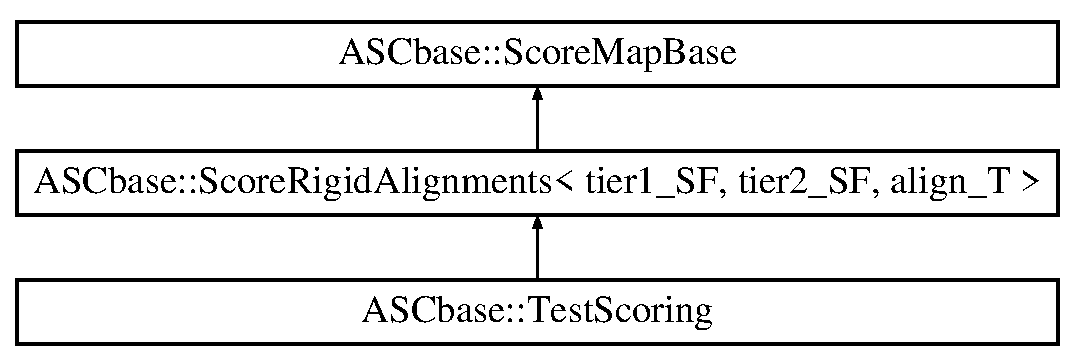
\includegraphics[height=3cm]{classASCbase_1_1TestScoring}
\end{center}
\end{figure}
\subsection*{Public Member Functions}
\begin{CompactItemize}
\item 
\bf{Test\-Scoring} (\bf{Model\-Sitemap} $\ast$model\_\-in, const \bf{Search\-Parameters} \&params)
\begin{CompactList}\small\item\em Default constructor for scoring methods of rigidly aligned sitemaps. \item\end{CompactList}\item 
\bf{$\sim$Test\-Scoring} ()\label{classASCbase_1_1TestScoring_47bf11af16fb49567855096808ec8a7f}

\begin{CompactList}\small\item\em basic destruction \item\end{CompactList}\end{CompactItemize}
\subsection*{Protected Member Functions}
\begin{CompactItemize}
\item 
my\_\-float\_\-t \bf{score} (const \bf{Dbase\-Sitemap} \&search, rigid\_\-align\_\-vi scores)
\begin{CompactList}\small\item\em Given an alignment of search to the query, score said alignment. \item\end{CompactList}\item 
my\_\-float\_\-t \textbf{correspondences} (my\_\-float\_\-t $\ast$$\ast$query\_\-pts\_\-ptr, my\_\-float\_\-t $\ast$$\ast$db\_\-pts\_\-ptr, size\_\-t $\ast$npts)\label{classASCbase_1_1TestScoring_1bce69b267b72ae43cd980caa7fcfd0e}

\end{CompactItemize}
\subsection*{Static Private Attributes}
\begin{CompactItemize}
\item 
static const std::string \bf{\_\-fname} = \char`\"{}Test\-Scoring.C\char`\"{}\label{classASCbase_1_1TestScoring_b4ebe268b1b74f5fe669c109de103c8f}

\begin{CompactList}\small\item\em \char`\"{}Weighted\-Sums\-Score.C\char`\"{} \item\end{CompactList}\item 
static const my\_\-float\_\-t \bf{POLAR\_\-SUM\_\-W} = -0.0140894\label{classASCbase_1_1TestScoring_d98e1f35e2bdf736d103e6e5b0acb5dd}

\begin{CompactList}\small\item\em -10370 \item\end{CompactList}\item 
static const my\_\-float\_\-t \bf{HPHOBIC\_\-COUNT\_\-W} = 0\label{classASCbase_1_1TestScoring_4d97cb87f8816169344f99d6d82f9910}

\begin{CompactList}\small\item\em -4130 \item\end{CompactList}\item 
static const my\_\-float\_\-t \bf{POLAR\_\-MISMATCH\_\-W} = 0\label{classASCbase_1_1TestScoring_346e2d0eab2f073e92340f747237e674}

\begin{CompactList}\small\item\em 11428 \item\end{CompactList}\item 
static const my\_\-float\_\-t \bf{UNSAT\_\-POLAR\_\-W} = 0\label{classASCbase_1_1TestScoring_668c7fb952beb31eb9c991e0f736570c}

\begin{CompactList}\small\item\em 963 \item\end{CompactList}\item 
static const my\_\-float\_\-t \bf{CONSTANT\_\-TERM} = -0.124725\label{classASCbase_1_1TestScoring_1ee5151bf6450adf872d86f51b9f9e72}

\begin{CompactList}\small\item\em -58070 \item\end{CompactList}\item 
static const my\_\-float\_\-t \bf{max\_\-dist} = 1.5\label{classASCbase_1_1TestScoring_46212ce7b93b0912702739bfd3efe04f}

\begin{CompactList}\small\item\em 1.5 angstroms \item\end{CompactList}\end{CompactItemize}


\subsection{Detailed Description}
Base class for scoring rigid alignments of dbase sitemaps to a given model. 



\subsection{Constructor \& Destructor Documentation}
\index{ASCbase::TestScoring@{ASCbase::Test\-Scoring}!TestScoring@{TestScoring}}
\index{TestScoring@{TestScoring}!ASCbase::TestScoring@{ASCbase::Test\-Scoring}}
\subsubsection{\setlength{\rightskip}{0pt plus 5cm}Test\-Scoring::Test\-Scoring (\bf{Model\-Sitemap} $\ast$ {\em model\_\-in}, const \bf{Search\-Parameters} \& {\em params})}\label{classASCbase_1_1TestScoring_30cc41f637641ce6dd0c225594e17e15}


Default constructor for scoring methods of rigidly aligned sitemaps. 

\begin{Desc}
\item[Parameters:]
\begin{description}
\item[{\em model\_\-in}]Pointer to the model points (sitemap class) \item[{\em params}]Reference to the search's runtime parameters \end{description}
\end{Desc}


\subsection{Member Function Documentation}
\index{ASCbase::TestScoring@{ASCbase::Test\-Scoring}!score@{score}}
\index{score@{score}!ASCbase::TestScoring@{ASCbase::Test\-Scoring}}
\subsubsection{\setlength{\rightskip}{0pt plus 5cm}my\_\-float\_\-t Test\-Scoring::score (const \bf{Dbase\-Sitemap} \& {\em search}, rigid\_\-align\_\-vi {\em scores})\hspace{0.3cm}{\tt  [protected]}}\label{classASCbase_1_1TestScoring_e0e06721302874c8daff87995f2609b9}


Given an alignment of search to the query, score said alignment. 

\begin{Desc}
\item[Parameters:]
\begin{description}
\item[{\em search}]Pointer to the sitemap aligned to the model sitemap \end{description}
\end{Desc}
\begin{Desc}
\item[Returns:]The score of the alignment \end{Desc}


The documentation for this class was generated from the following files:\begin{CompactItemize}
\item 
TESTSCORING.H\item 
TESTSCORING.C\end{CompactItemize}

\section{ASCbase::Timer Class Reference}
\label{classASCbase_1_1Timer}\index{ASCbase::Timer@{ASCbase::Timer}}
A Linux profile timer for sequential programs.  


{\tt \#include $<$Timer.H$>$}

\subsection*{Public Member Functions}
\begin{CompactItemize}
\item 
\bf{Timer} (int interval\_\-sec\_\-in=10)
\begin{CompactList}\small\item\em Constructor, sets the timer interval. \item\end{CompactList}\item 
\bf{$\sim$Timer} ()\label{classASCbase_1_1Timer_cd15e84294d41860cdd7a3094d3f44e3}

\begin{CompactList}\small\item\em Do nothing destructor. \item\end{CompactList}\item 
bool \bf{start} ()
\begin{CompactList}\small\item\em Starts profile timer. \item\end{CompactList}\item 
bool \bf{get} (double $\ast$real, double $\ast$virt, double $\ast$prof)
\begin{CompactList}\small\item\em Gets the elapsed time in seconds. \item\end{CompactList}\item 
bool \bf{fail} ()\label{classASCbase_1_1Timer_f493887703b0b619373eed9601c2d517}

\begin{CompactList}\small\item\em True if an error had occured. \item\end{CompactList}\item 
bool \bf{started} ()
\end{CompactItemize}
\subsection*{Static Public Member Functions}
\begin{CompactItemize}
\item 
static std::string \bf{get\_\-local\_\-time} (char $\ast$buf, size\_\-t buf\_\-len)
\begin{CompactList}\small\item\em Get the local time in a string format. \item\end{CompactList}\item 
static void \bf{sig\_\-handler} (int signum, siginfo\_\-t $\ast$siginfo, void $\ast$ucontext)
\begin{CompactList}\small\item\em The sig handler used when the timer expires. \item\end{CompactList}\end{CompactItemize}
\subsection*{Private Member Functions}
\begin{CompactItemize}
\item 
\bf{Timer} (const \bf{Timer} \&)
\begin{CompactList}\small\item\em Privatized copy constructor. \item\end{CompactList}\item 
bool \bf{get\_\-itimer} (double $\ast$rv, int which, long elapsed\_\-sec)\label{classASCbase_1_1Timer_9de292b90dfbc1e13c935e142d5925a0}

\begin{CompactList}\small\item\em Get the elapsed time for \char`\"{}which\char`\"{} timer in seconds. \item\end{CompactList}\end{CompactItemize}
\subsection*{Static Private Member Functions}
\begin{CompactItemize}
\item 
static size\_\-t \bf{my\_\-strftime} (char $\ast$s, size\_\-t max, const char $\ast$fmt, const struct tm $\ast$tm)
\begin{CompactList}\small\item\em Wrapper to eliminate buggy gcc warning about using \char`\"{}\%c\char`\"{} in strftime. \item\end{CompactList}\end{CompactItemize}
\subsection*{Private Attributes}
\begin{CompactItemize}
\item 
bool \bf{A\_\-fail}\label{classASCbase_1_1Timer_7609083d78f0745bb5bcbf0901e9bcc2}

\begin{CompactList}\small\item\em False implies no outstanding errors. \item\end{CompactList}\item 
bool \bf{A\_\-started}\label{classASCbase_1_1Timer_213642a43dde180cf72016bd4d42a344}

\begin{CompactList}\small\item\em True implies timers are running. \item\end{CompactList}\end{CompactItemize}
\subsection*{Static Private Attributes}
\begin{CompactItemize}
\item 
static long \bf{A\_\-timer\_\-interval\_\-sec} = 0\label{classASCbase_1_1Timer_a9d182c83c64a1f2736ed6db96ff4d5b}

\begin{CompactList}\small\item\em Number of sec used to init a timer. \item\end{CompactList}\item 
static long \bf{A\_\-real\_\-elapsed\_\-sec} = 0\label{classASCbase_1_1Timer_6198dfbf30712f92ba60374bdc7fb446}

\begin{CompactList}\small\item\em real elapsed time not including timer \item\end{CompactList}\item 
static long \bf{A\_\-virt\_\-elapsed\_\-sec} = 0\label{classASCbase_1_1Timer_641a06b85a83c8bfe6b5c868ef015160}

\begin{CompactList}\small\item\em virtual elapsed time not including timer \item\end{CompactList}\item 
static long \bf{A\_\-prof\_\-elapsed\_\-sec} = 0\label{classASCbase_1_1Timer_cd7832452dd43df2c4b55fad0d67f74c}

\begin{CompactList}\small\item\em profile elapsed time not including timer \item\end{CompactList}\end{CompactItemize}


\subsection{Detailed Description}
A Linux profile timer for sequential programs. 

This class has been updated to use sigaction() in the place of signal(). 



\subsection{Constructor \& Destructor Documentation}
\index{ASCbase::Timer@{ASCbase::Timer}!Timer@{Timer}}
\index{Timer@{Timer}!ASCbase::Timer@{ASCbase::Timer}}
\subsubsection{\setlength{\rightskip}{0pt plus 5cm}Timer::Timer (int {\em interval\_\-sec\_\-in} = {\tt 10})}\label{classASCbase_1_1Timer_122d59508cd380085fc87dc1755d4179}


Constructor, sets the timer interval. 

Sets the timer interval and initial timer to timer\_\-interval\_\-in

\begin{Desc}
\item[Parameters:]
\begin{description}
\item[{\em interval\_\-sec\_\-in}]Value for timer interval an initial timer \end{description}
\end{Desc}
\index{ASCbase::Timer@{ASCbase::Timer}!Timer@{Timer}}
\index{Timer@{Timer}!ASCbase::Timer@{ASCbase::Timer}}
\subsubsection{\setlength{\rightskip}{0pt plus 5cm}ASCbase::Timer::Timer (const \bf{Timer} \&)\hspace{0.3cm}{\tt  [inline, private]}}\label{classASCbase_1_1Timer_2b55a2346ab31964a25cb65907e62e99}


Privatized copy constructor. 

There is no valid reason to copy a timer class 

\subsection{Member Function Documentation}
\index{ASCbase::Timer@{ASCbase::Timer}!get@{get}}
\index{get@{get}!ASCbase::Timer@{ASCbase::Timer}}
\subsubsection{\setlength{\rightskip}{0pt plus 5cm}bool Timer::get (double $\ast$ {\em real}, double $\ast$ {\em virt}, double $\ast$ {\em prof})}\label{classASCbase_1_1Timer_7943ae280c460242a3bb4c896ad80223}


Gets the elapsed time in seconds. 

\begin{Desc}
\item[Parameters:]
\begin{description}
\item[{\em real}]Ptr to loc to store the elapsed real time \item[{\em virt}]Ptr to loc to store the elapsed virtual time \item[{\em prof}]Ptr to loc to store the elapsed profile time \end{description}
\end{Desc}
\begin{Desc}
\item[Returns:]True if !fail() and \doxyref{started()}{p.}{classASCbase_1_1Timer_e0aa8a339712737f79406a38a2aa3258} \end{Desc}
\index{ASCbase::Timer@{ASCbase::Timer}!get_local_time@{get\_\-local\_\-time}}
\index{get_local_time@{get\_\-local\_\-time}!ASCbase::Timer@{ASCbase::Timer}}
\subsubsection{\setlength{\rightskip}{0pt plus 5cm}std::string Timer::get\_\-local\_\-time (char $\ast$ {\em buf}, size\_\-t {\em buf\_\-len})\hspace{0.3cm}{\tt  [static]}}\label{classASCbase_1_1Timer_4201c600a36475ddfeefa6def6aa610c}


Get the local time in a string format. 

Does not necessarily belong in the \doxyref{Timer}{p.}{classASCbase_1_1Timer} class, but currently this is as good a place as any.

\begin{Desc}
\item[Parameters:]
\begin{description}
\item[{\em buf}]A Cstring used in the call to strftime \item[{\em buf\_\-len}]Length of the Cstring buf \end{description}
\end{Desc}
\begin{Desc}
\item[Returns:]A string holding the broken down format of the local time. \end{Desc}
\index{ASCbase::Timer@{ASCbase::Timer}!my_strftime@{my\_\-strftime}}
\index{my_strftime@{my\_\-strftime}!ASCbase::Timer@{ASCbase::Timer}}
\subsubsection{\setlength{\rightskip}{0pt plus 5cm}static size\_\-t ASCbase::Timer::my\_\-strftime (char $\ast$ {\em s}, size\_\-t {\em max}, const char $\ast$ {\em fmt}, const struct tm $\ast$ {\em tm})\hspace{0.3cm}{\tt  [inline, static, private]}}\label{classASCbase_1_1Timer_e1235f2eabcca3f12ff7c61225bb7210}


Wrapper to eliminate buggy gcc warning about using \char`\"{}\%c\char`\"{} in strftime. 

From the man page for strftime: Some buggy versions of gcc complain about the use of c: warning: `c' yields only last 2 digits of year in some locales. Of course programmers are encouraged to use c, it gives the preferred date and time representation. One meets all kinds of strange obfuscations to circumvent this gcc problem. A relatively clean one is to add this intermediate function.

\begin{Desc}
\item[Parameters:]
\begin{description}
\item[{\em s}]Character array of size max \item[{\em max}]Size of the array s \item[{\em fmt}]Format string \item[{\em tm}]The tm structure to convert to a string. \end{description}
\end{Desc}
\begin{Desc}
\item[Returns:]The number of chars written to s if the time fits, else 0. \end{Desc}
\index{ASCbase::Timer@{ASCbase::Timer}!sig_handler@{sig\_\-handler}}
\index{sig_handler@{sig\_\-handler}!ASCbase::Timer@{ASCbase::Timer}}
\subsubsection{\setlength{\rightskip}{0pt plus 5cm}void Timer::sig\_\-handler (int {\em signum}, siginfo\_\-t $\ast$ {\em siginfo}, void $\ast$ {\em ucontext})\hspace{0.3cm}{\tt  [static]}}\label{classASCbase_1_1Timer_914aeaeacb811e85d426ae2867c9bc30}


The sig handler used when the timer expires. 

\begin{Desc}
\item[Parameters:]
\begin{description}
\item[{\em signum}]The signal number passed to the sig handler \item[{\em siginfo}]Pointer to a siginfo\_\-t struct -- ignored by this function \item[{\em ucontext}]Void pointer to a ucontext\_\-t -- ignored by this function \end{description}
\end{Desc}
\index{ASCbase::Timer@{ASCbase::Timer}!start@{start}}
\index{start@{start}!ASCbase::Timer@{ASCbase::Timer}}
\subsubsection{\setlength{\rightskip}{0pt plus 5cm}bool Timer::start ()}\label{classASCbase_1_1Timer_af02e2d4035c0e6c90223918e7b3c093}


Starts profile timer. 

\begin{Desc}
\item[Returns:]True if timer was started, else false \end{Desc}
\index{ASCbase::Timer@{ASCbase::Timer}!started@{started}}
\index{started@{started}!ASCbase::Timer@{ASCbase::Timer}}
\subsubsection{\setlength{\rightskip}{0pt plus 5cm}bool ASCbase::Timer::started ()\hspace{0.3cm}{\tt  [inline]}}\label{classASCbase_1_1Timer_e0aa8a339712737f79406a38a2aa3258}


True if timers have been started (i.e. \doxyref{start()}{p.}{classASCbase_1_1Timer_af02e2d4035c0e6c90223918e7b3c093} has been called successfully) 

The documentation for this class was generated from the following files:\begin{CompactItemize}
\item 
Timer.H\item 
Timer.C\end{CompactItemize}

\section{ASCbase::triangle\_\-t Struct Reference}
\label{structASCbase_1_1triangle__t}\index{ASCbase::triangle_t@{ASCbase::triangle\_\-t}}
A triangle has 3 labeled vertices and 3 edges.  


{\tt \#include $<$Model\-Sitemap.H$>$}

\subsection*{Public Attributes}
\begin{CompactItemize}
\item 
my\_\-float\_\-t \bf{edge\_\-len} [3]\label{structASCbase_1_1triangle__t_054eeaf8f6d93e76685c52338351cc40}

\begin{CompactList}\small\item\em Lengths of the triangle edges. \item\end{CompactList}\item 
interact\_\-pts\_\-vci \bf{vertices} [3]\label{structASCbase_1_1triangle__t_6c50fcf5765d863b447d3f85d2ed5bdb}

\begin{CompactList}\small\item\em Iterators to the vertices. \item\end{CompactList}\end{CompactItemize}


\subsection{Detailed Description}
A triangle has 3 labeled vertices and 3 edges. 



The documentation for this struct was generated from the following file:\begin{CompactItemize}
\item 
Model\-Sitemap.H\end{CompactItemize}

\section{ASCbase::geometry::triangle\_\-t Class Reference}
\label{classASCbase_1_1geometry_1_1triangle__t}\index{ASCbase::geometry::triangle_t@{ASCbase::geometry::triangle\_\-t}}
Requires \doxyref{vertex\_\-t}{p.}{classASCbase_1_1geometry_1_1vertex__t} class and should be independent of vertex placement.  


{\tt \#include $<$Tri\-Mesh\-Sphere.H$>$}

\subsection*{Public Member Functions}
\begin{CompactItemize}
\item 
\textbf{triangle\_\-t} (vertex\_\-vci a, vertex\_\-vci b, vertex\_\-vci c)\label{classASCbase_1_1geometry_1_1triangle__t_20cf34d2980bcba176b5f1a5974c9949}

\item 
\textbf{triangle\_\-t} (const \bf{triangle\_\-t} \&src)\label{classASCbase_1_1geometry_1_1triangle__t_6a32e06433ed8f97deba97528f2fc9eb}

\item 
const \bf{triangle\_\-t} \& \textbf{operator=} (const \bf{triangle\_\-t} \&src)\label{classASCbase_1_1geometry_1_1triangle__t_6b7f6f294ca61e81be773c4d94955caf}

\item 
bool \bf{contains} (const my\_\-float\_\-t $\ast$pt) const 
\item 
my\_\-float\_\-t \bf{face\_\-normal} (my\_\-float\_\-t $\ast$N)\label{classASCbase_1_1geometry_1_1triangle__t_5331997a2c7ee3c5f772d46e8e1a860c}

\begin{CompactList}\small\item\em Compute the normal to the out facing triangle face. \item\end{CompactList}\item 
std::vector$<$ vertex\_\-vci $>$::const\_\-iterator \textbf{vertices\_\-begin} () const \label{classASCbase_1_1geometry_1_1triangle__t_bbe6598e0017fb18899416403e149ff1}

\item 
std::vector$<$ vertex\_\-vci $>$::const\_\-iterator \textbf{vertices\_\-end} () const \label{classASCbase_1_1geometry_1_1triangle__t_295db5679d4a1a34fa659942226a1a2a}

\item 
my\_\-float\_\-t \textbf{area} () const \label{classASCbase_1_1geometry_1_1triangle__t_02c5681d05a731dfe88150aceacedd0c}

\end{CompactItemize}
\subsection*{Private Member Functions}
\begin{CompactItemize}
\item 
bool \bf{contains} (const my\_\-float\_\-t $\ast$x, const my\_\-float\_\-t $\ast$y) const 
\begin{CompactList}\small\item\em 2D version \item\end{CompactList}\item 
void \textbf{do\_\-copy} (const \bf{triangle\_\-t} \&src)\label{classASCbase_1_1geometry_1_1triangle__t_53cc9666d4f501fc21bd146d2a94fe48}

\end{CompactItemize}
\subsection*{Private Attributes}
\begin{CompactItemize}
\item 
std::vector$<$ vertex\_\-vci $>$ \bf{A\_\-vertices}\label{classASCbase_1_1geometry_1_1triangle__t_c8cfb8905953a26c172c9c6b83f51d6a}

\begin{CompactList}\small\item\em 3 vertices of the triangle \item\end{CompactList}\item 
my\_\-float\_\-t \bf{A\_\-area}\label{classASCbase_1_1geometry_1_1triangle__t_e7585186eb0d6f2016c076237d872e1c}

\begin{CompactList}\small\item\em Area of the triangle. \item\end{CompactList}\end{CompactItemize}


\subsection{Detailed Description}
Requires \doxyref{vertex\_\-t}{p.}{classASCbase_1_1geometry_1_1vertex__t} class and should be independent of vertex placement. 

Since this class is supposed to be independent of the vertices positions and normals, it is currently the users reponsibility to insure that the vertices and triangle are consistent. 



\subsection{Member Function Documentation}
\index{ASCbase::geometry::triangle_t@{ASCbase::geometry::triangle\_\-t}!contains@{contains}}
\index{contains@{contains}!ASCbase::geometry::triangle_t@{ASCbase::geometry::triangle\_\-t}}
\subsubsection{\setlength{\rightskip}{0pt plus 5cm}bool ASCbase::geometry::triangle\_\-t::contains (const my\_\-float\_\-t $\ast$ {\em x}, const my\_\-float\_\-t $\ast$ {\em y}) const\hspace{0.3cm}{\tt  [inline, private]}}\label{classASCbase_1_1geometry_1_1triangle__t_c0169da86ab7cf87febd87bec91456e8}


2D version 

From Usenet discussion on Barycentric Coordinates (Joseph O'Rourke, 1992) NOTE: for now, this function requires the points be ordered in a counterclockwise fashion \index{ASCbase::geometry::triangle_t@{ASCbase::geometry::triangle\_\-t}!contains@{contains}}
\index{contains@{contains}!ASCbase::geometry::triangle_t@{ASCbase::geometry::triangle\_\-t}}
\subsubsection{\setlength{\rightskip}{0pt plus 5cm}bool ASCbase::geometry::triangle\_\-t::contains (const my\_\-float\_\-t $\ast$ {\em pt}) const\hspace{0.3cm}{\tt  [inline]}}\label{classASCbase_1_1geometry_1_1triangle__t_e206410f4050312797009de5d6e3696d}


3D version that drops the coordinate with the least variance and calls the 2D method 

The documentation for this class was generated from the following file:\begin{CompactItemize}
\item 
Tri\-Mesh\-Sphere.H\end{CompactItemize}

\section{ASCbase::geometry::Tri\-Mesh\-Sphere Class Reference}
\label{classASCbase_1_1geometry_1_1TriMeshSphere}\index{ASCbase::geometry::TriMeshSphere@{ASCbase::geometry::TriMeshSphere}}
{\tt \#include $<$Tri\-Mesh\-Sphere.H$>$}

\subsection*{Public Types}
\begin{CompactItemize}
\item 
typedef enum \bf{ASCbase::geometry::Tri\-Mesh\-Sphere::sphere\_\-init\_\-type} \bf{sphere\_\-init\_\-t}\label{classASCbase_1_1geometry_1_1TriMeshSphere_adaa2f3ea546c14705877efaba422ac5}

\begin{CompactList}\small\item\em More descriptive method to denote initialization type for spherical mesh. \item\end{CompactList}\item 
\textbf{FULL\_\-SPHERE}\label{classASCbase_1_1geometry_1_1TriMeshSphere_1b7e3821daf89de36b78b79203a320545ca923ad9ce9681e6173252423882a51}

\item 
\textbf{SPHERICAL\_\-CAP}\label{classASCbase_1_1geometry_1_1TriMeshSphere_1b7e3821daf89de36b78b79203a3205441ddb124c602b61ac0a60de93ddc2f7d}

\item 
enum \bf{sphere\_\-init\_\-type} \{ \textbf{FULL\_\-SPHERE}, 
\textbf{SPHERICAL\_\-CAP}
 \}
\begin{CompactList}\small\item\em More descriptive method to denote initialization type for spherical mesh. \item\end{CompactList}\end{CompactItemize}
\subsection*{Public Member Functions}
\begin{CompactItemize}
\item 
\bf{Tri\-Mesh\-Sphere} ()
\item 
\bf{Tri\-Mesh\-Sphere} (const my\_\-float\_\-t $\ast$R, const my\_\-float\_\-t $\ast$T, const my\_\-float\_\-t $\ast$dir, const \bf{sphere\_\-init\_\-t} init\_\-obj, const my\_\-float\_\-t radius=3.0, const uint level=2)
\item 
\textbf{Tri\-Mesh\-Sphere} (const \bf{Tri\-Mesh\-Sphere} \&src)\label{classASCbase_1_1geometry_1_1TriMeshSphere_b6396ee2c69154d55a327987b04c56b7}

\item 
\bf{Tri\-Mesh\-Sphere} \& \textbf{operator=} (const \bf{Tri\-Mesh\-Sphere} \&src)\label{classASCbase_1_1geometry_1_1TriMeshSphere_285b18dae29b3919d6516ced3f4a861c}

\item 
void \textbf{transform} (const my\_\-float\_\-t $\ast$R, const my\_\-float\_\-t $\ast$T)\label{classASCbase_1_1geometry_1_1TriMeshSphere_9e9bf1d856a40799f6fa385f8192427b}

\item 
void \textbf{inverse\_\-transform} (const my\_\-float\_\-t $\ast$R, const my\_\-float\_\-t $\ast$T)\label{classASCbase_1_1geometry_1_1TriMeshSphere_6a11da9e82a8ba89afb1ceaec4fd5e3e}

\item 
void \textbf{revert} ()\label{classASCbase_1_1geometry_1_1TriMeshSphere_baa72acd8f2096aa9995855d5d8c1375}

\item 
void \textbf{adjust\_\-points} (\bf{hbond\_\-surface\_\-t} \&surf)\label{classASCbase_1_1geometry_1_1TriMeshSphere_a550da12f3d525e8dc9472bb5c590fb8}

\item 
my\_\-float\_\-t \textbf{complementary\_\-surface\_\-area} (const std::map$<$ vertex\_\-vci, bool $>$ \&kept\_\-vertices) const \label{classASCbase_1_1geometry_1_1TriMeshSphere_453ba64dab8da3831126f9d89c948db6}

\item 
const vertex\_\-vci \bf{verts\_\-begin} () const \label{classASCbase_1_1geometry_1_1TriMeshSphere_3ee17324150856a0629eaf5eac7a388c}

\begin{CompactList}\small\item\em Get a constant iterator to the first vertex in the vector. \item\end{CompactList}\item 
const vertex\_\-vci \bf{verts\_\-end} () const \label{classASCbase_1_1geometry_1_1TriMeshSphere_edc98936bdb42ffbf98656b8caa6595a}

\begin{CompactList}\small\item\em Get a constant iterator to the end of the vertex vector. \item\end{CompactList}\item 
const uint \bf{num\_\-verts} () const \label{classASCbase_1_1geometry_1_1TriMeshSphere_8835cfe88ab71442635ab7d5f05c4767}

\begin{CompactList}\small\item\em Get the number of vertices in the surface. \item\end{CompactList}\item 
void \bf{write} (std::ostream \&out, const interaction\-Type act\_\-type, const char delim='$|$') const \label{classASCbase_1_1geometry_1_1TriMeshSphere_dd30e7e90a9f41be6d54de06cba3d0f0}

\begin{CompactList}\small\item\em Write out the triangles in the mesh. \item\end{CompactList}\item 
void \textbf{write\_\-msms\_\-headers} (std::ostream \&vert\_\-out, std::ostream \&face\_\-out) const \label{classASCbase_1_1geometry_1_1TriMeshSphere_b3552eec82a823e41ef9ed70504b7368}

\item 
void \textbf{write\_\-msms\_\-cap} (std::ostream \&vert\_\-out, std::ostream \&face\_\-out, const interaction\-Type act\_\-type) const \label{classASCbase_1_1geometry_1_1TriMeshSphere_3772f4f815c191e7fe24cca03e8f96e9}

\end{CompactItemize}
\subsection*{Private Member Functions}
\begin{CompactItemize}
\item 
void \textbf{init} ()\label{classASCbase_1_1geometry_1_1TriMeshSphere_08a7be3e5e7bed201fa7f24da0d18b47}

\item 
void \bf{do\_\-copy} (const \bf{Tri\-Mesh\-Sphere} \&src)\label{classASCbase_1_1geometry_1_1TriMeshSphere_140990c6bc17c7f0f46950c2262fe0e5}

\begin{CompactList}\small\item\em The function that does all the work for copying the class. \item\end{CompactList}\item 
void \textbf{set\_\-global\_\-pos} (const my\_\-float\_\-t $\ast$R, const my\_\-float\_\-t $\ast$T, const my\_\-float\_\-t $\ast$bond\_\-dir)\label{classASCbase_1_1geometry_1_1TriMeshSphere_dd481c24ae86c6ccab7eae4965d44beb}

\item 
void \textbf{init\_\-storages} (const my\_\-float\_\-t $\ast$pts, const uint npts, const uint $\ast$triangles, const uint ntris, const my\_\-float\_\-t radius)\label{classASCbase_1_1geometry_1_1TriMeshSphere_19b9aa460a8c48a1ebe6eff1c0ecee43}

\item 
void \textbf{A\_\-adjust\_\-points} (\bf{hbond\_\-surface\_\-t} \&surf, const uint $\ast$tri\_\-vert\_\-idz, const uint num\_\-tris)\label{classASCbase_1_1geometry_1_1TriMeshSphere_3cbe2b20213813abb31e070f5898d7b2}

\item 
void \textbf{add\_\-triangle} (const uint $\ast$idz)\label{classASCbase_1_1geometry_1_1TriMeshSphere_533c34ac5b9c4435802391c6e5329048}

\item 
void \textbf{setup\_\-vert\_\-to\_\-deltas\_\-map} ()\label{classASCbase_1_1geometry_1_1TriMeshSphere_bba5d7fbb2e79443cf7294b0fed4662c}

\end{CompactItemize}
\subsection*{Private Attributes}
\begin{CompactItemize}
\item 
const my\_\-float\_\-t $\ast$ \textbf{A\_\-local\_\-points}\label{classASCbase_1_1geometry_1_1TriMeshSphere_7ace9bbea8fff45d3dfb5d915adb664e}

\item 
uint \textbf{A\_\-npts}\label{classASCbase_1_1geometry_1_1TriMeshSphere_098883f74c0eed5ecc66f428f48d70a0}

\item 
const uint $\ast$ \textbf{A\_\-triangles}\label{classASCbase_1_1geometry_1_1TriMeshSphere_af90c5e36bec515b764a6394ba50ac4a}

\item 
uint \textbf{A\_\-num\_\-tris}\label{classASCbase_1_1geometry_1_1TriMeshSphere_0775a1f564a7b75cda3723d1a4806ceb}

\item 
\bf{dir\_\-point\_\-storage}$<$ \bf{vertex\_\-t} $>$ \textbf{A\_\-nodes}\label{classASCbase_1_1geometry_1_1TriMeshSphere_dbc874022d8fcc737354707cfaccb77d}

\item 
triangle\_\-vec \textbf{A\_\-deltas}\label{classASCbase_1_1geometry_1_1TriMeshSphere_d5d4d2dcd06c55fc25e58b49be8c2de3}

\item 
std::map$<$ vertex\_\-vci, std::vector$<$ triangle\_\-vci $>$ $>$ \textbf{A\_\-verts\_\-to\_\-deltas\_\-map}\label{classASCbase_1_1geometry_1_1TriMeshSphere_bfb7fca04fe4b2c9245035607914dd47}

\item 
half\_\-edge\_\-vec \textbf{A\_\-half\_\-edges}\label{classASCbase_1_1geometry_1_1TriMeshSphere_f808f7f4a48e4ad6ee7b24a1002fdfbd}

\end{CompactItemize}
\subsection*{Static Private Attributes}
\begin{CompactItemize}
\item 
static const my\_\-float\_\-t \textbf{A\_\-level1\_\-sphere\_\-points} [$\,$]
\item 
static const uint \textbf{A\_\-level1\_\-sphere\_\-npts} = 22\label{classASCbase_1_1geometry_1_1TriMeshSphere_6c2549e9daacf27c7cf15cb3eb7b7373}

\item 
static const uint \textbf{A\_\-level1\_\-sphere\_\-triangles} [$\,$]\label{classASCbase_1_1geometry_1_1TriMeshSphere_278a1d74c086e8ebc40ef05d74b9ea15}

\item 
static const uint \textbf{A\_\-level1\_\-num\_\-sphere\_\-tris} = 40\label{classASCbase_1_1geometry_1_1TriMeshSphere_e42055072b403bf91bb04dfe81b8a77c}

\item 
static const my\_\-float\_\-t \textbf{A\_\-level2\_\-sphere\_\-points} [$\,$]\label{classASCbase_1_1geometry_1_1TriMeshSphere_9218b68dfd06e39789b926138618dfeb}

\item 
static const uint \textbf{A\_\-level2\_\-sphere\_\-npts} = 82\label{classASCbase_1_1geometry_1_1TriMeshSphere_6c493b2654c01b707878f88a76cb12bb}

\item 
static const uint \textbf{A\_\-level2\_\-sphere\_\-triangles} [$\,$]\label{classASCbase_1_1geometry_1_1TriMeshSphere_334f79d29df15c86e07a9b2f771436b5}

\item 
static const uint \textbf{A\_\-level2\_\-num\_\-sphere\_\-tris} = 160\label{classASCbase_1_1geometry_1_1TriMeshSphere_e8608fc384f66ad810567214a8a65328}

\item 
static const my\_\-float\_\-t \textbf{A\_\-level2\_\-cap\_\-points} [$\,$]
\item 
static const uint \textbf{A\_\-level2\_\-cap\_\-npts} = 16\label{classASCbase_1_1geometry_1_1TriMeshSphere_72717de0132dc9de41615e95777e78d1}

\item 
static const uint \textbf{A\_\-level2\_\-cap\_\-triangles} [$\,$]
\item 
static const uint \textbf{A\_\-level2\_\-num\_\-cap\_\-tris} = 20\label{classASCbase_1_1geometry_1_1TriMeshSphere_852532701e612513420c5cfcee27edfc}

\end{CompactItemize}


\subsection{Detailed Description}
Straightforward class to work with a mesh sphere that has portions of it occluded 



\subsection{Constructor \& Destructor Documentation}
\index{ASCbase::geometry::TriMeshSphere@{ASCbase::geometry::Tri\-Mesh\-Sphere}!TriMeshSphere@{TriMeshSphere}}
\index{TriMeshSphere@{TriMeshSphere}!ASCbase::geometry::TriMeshSphere@{ASCbase::geometry::Tri\-Mesh\-Sphere}}
\subsubsection{\setlength{\rightskip}{0pt plus 5cm}ASCbase::geometry::Tri\-Mesh\-Sphere::Tri\-Mesh\-Sphere ()\hspace{0.3cm}{\tt  [inline]}}\label{classASCbase_1_1geometry_1_1TriMeshSphere_1e6bc0c8cf5b808ab92acbbf0648ac4c}


Default constructor -- allows class to be an object in another class before one knows the values for the sphere \index{ASCbase::geometry::TriMeshSphere@{ASCbase::geometry::Tri\-Mesh\-Sphere}!TriMeshSphere@{TriMeshSphere}}
\index{TriMeshSphere@{TriMeshSphere}!ASCbase::geometry::TriMeshSphere@{ASCbase::geometry::Tri\-Mesh\-Sphere}}
\subsubsection{\setlength{\rightskip}{0pt plus 5cm}Tri\-Mesh\-Sphere::Tri\-Mesh\-Sphere (const my\_\-float\_\-t $\ast$ {\em R}, const my\_\-float\_\-t $\ast$ {\em T}, const my\_\-float\_\-t $\ast$ {\em dir}, const \bf{sphere\_\-init\_\-t} {\em init\_\-obj}, const my\_\-float\_\-t {\em radius} = {\tt 3.0}, const uint {\em level} = {\tt 2})}\label{classASCbase_1_1geometry_1_1TriMeshSphere_e64b7ebd41fc3709a78a96c0ef36df88}


Constructor to generate a mesh representation of a sphere or part of sphere depending on the init\_\-obj variable. 

\subsection{Member Data Documentation}
\index{ASCbase::geometry::TriMeshSphere@{ASCbase::geometry::Tri\-Mesh\-Sphere}!A_level1_sphere_points@{A\_\-level1\_\-sphere\_\-points}}
\index{A_level1_sphere_points@{A\_\-level1\_\-sphere\_\-points}!ASCbase::geometry::TriMeshSphere@{ASCbase::geometry::Tri\-Mesh\-Sphere}}
\subsubsection{\setlength{\rightskip}{0pt plus 5cm}const my\_\-float\_\-t Tri\-Mesh\-Sphere::A\_\-level1\_\-sphere\_\-points\hspace{0.3cm}{\tt  [static, private]}}\label{classASCbase_1_1geometry_1_1TriMeshSphere_3f273941f74164c78f9338072e17f6e1}


\textbf{Initial value:}

\begin{Code}\begin{verbatim}
  { 0.707107,0.218508,0.672498,
    0.707107,0.707107,0.000000,
    0.000000,0.809017,0.587785,
    1.000000,0.000000,0.000000,
    0.000000,1.000000,0.000000,
    0.000000,0.309017,0.951056,
    -0.707107,0.218508,0.672498,
    -0.707107,0.707107,0.000000,
    -1.000000,0.000000,0.000000,
    0.707107,-0.572061,0.415627,
    0.000000,-0.309017,0.951056,
    0.000000,-0.809017,0.587785,
    -0.707107,-0.572061,0.415627,
    0.707107,-0.572061,-0.415627,
    0.000000,-1.000000,0.000000,
    0.000000,-0.809017,-0.587785,
    -0.707107,-0.572061,-0.415627,
    0.707107,0.218508,-0.672498,
    0.000000,-0.309017,-0.951056,
    0.000000,0.309017,-0.951056,
    -0.707107,0.218508,-0.672498,
    0.000000,0.809017,-0.587785
  }
\end{verbatim}\end{Code}
\index{ASCbase::geometry::TriMeshSphere@{ASCbase::geometry::Tri\-Mesh\-Sphere}!A_level2_cap_points@{A\_\-level2\_\-cap\_\-points}}
\index{A_level2_cap_points@{A\_\-level2\_\-cap\_\-points}!ASCbase::geometry::TriMeshSphere@{ASCbase::geometry::Tri\-Mesh\-Sphere}}
\subsubsection{\setlength{\rightskip}{0pt plus 5cm}const my\_\-float\_\-t Tri\-Mesh\-Sphere::A\_\-level2\_\-cap\_\-points\hspace{0.3cm}{\tt  [static, private]}}\label{classASCbase_1_1geometry_1_1TriMeshSphere_a007ec03a3a5930ee56566c87f2a2772}


\textbf{Initial value:}

\begin{Code}\begin{verbatim}
  { 0.866025,0.154508,0.475528,
    0.866025,0.500000,0.000000,
    0.500000,0.700629,0.509037,
    1.000000,0.000000,0.000000,
    0.500000,0.866025,0.000000,
    0.500000,0.267617,0.823639,
    0.866025,-0.404508,0.293893,
    0.500000,-0.267617,0.823639,
    0.500000,-0.700629,0.509037,
    0.866025,-0.404508,-0.293893,
    0.500000,-0.866025,0.000000,
    0.500000,-0.700629,-0.509037,
    0.866025,0.154508,-0.475528,
    0.500000,-0.267617,-0.823639,
    0.500000,0.267617,-0.823639,
    0.500000,0.700629,-0.509037
  }
\end{verbatim}\end{Code}
\index{ASCbase::geometry::TriMeshSphere@{ASCbase::geometry::Tri\-Mesh\-Sphere}!A_level2_cap_triangles@{A\_\-level2\_\-cap\_\-triangles}}
\index{A_level2_cap_triangles@{A\_\-level2\_\-cap\_\-triangles}!ASCbase::geometry::TriMeshSphere@{ASCbase::geometry::Tri\-Mesh\-Sphere}}
\subsubsection{\setlength{\rightskip}{0pt plus 5cm}const uint Tri\-Mesh\-Sphere::A\_\-level2\_\-cap\_\-triangles\hspace{0.3cm}{\tt  [static, private]}}\label{classASCbase_1_1geometry_1_1TriMeshSphere_58db5fd91484c9fd014384310be33341}


\textbf{Initial value:}

\begin{Code}\begin{verbatim} 
  { 0,1,2,
    3,1,0,
    4,2,1,
    5,0,2,
    6,0,7,
    3,0,6,
    5,7,0,
    8,6,7,
    9,6,10,
    3,6,9,
    8,10,6,
    11,9,10,
    12,9,13,
    3,9,12,
    11,13,9,
    14,12,13,
    1,12,15,
    3,12,1,
    14,15,12,
    4,1,15,
  }
\end{verbatim}\end{Code}


The documentation for this class was generated from the following files:\begin{CompactItemize}
\item 
Tri\-Mesh\-Sphere.H\item 
Tri\-Mesh\-Sphere.C\end{CompactItemize}

\section{ASCbase::geometry::two\_\-thirds\_\-triangle Class Reference}
\label{classASCbase_1_1geometry_1_1two__thirds__triangle}\index{ASCbase::geometry::two_thirds_triangle@{ASCbase::geometry::two\_\-thirds\_\-triangle}}
Simple derived class that gives us a unique number for 2/3rds of triangle.  


{\tt \#include $<$Immovable\-Trimesh.H$>$}

Inheritance diagram for ASCbase::geometry::two\_\-thirds\_\-triangle::\begin{figure}[H]
\begin{center}
\leavevmode
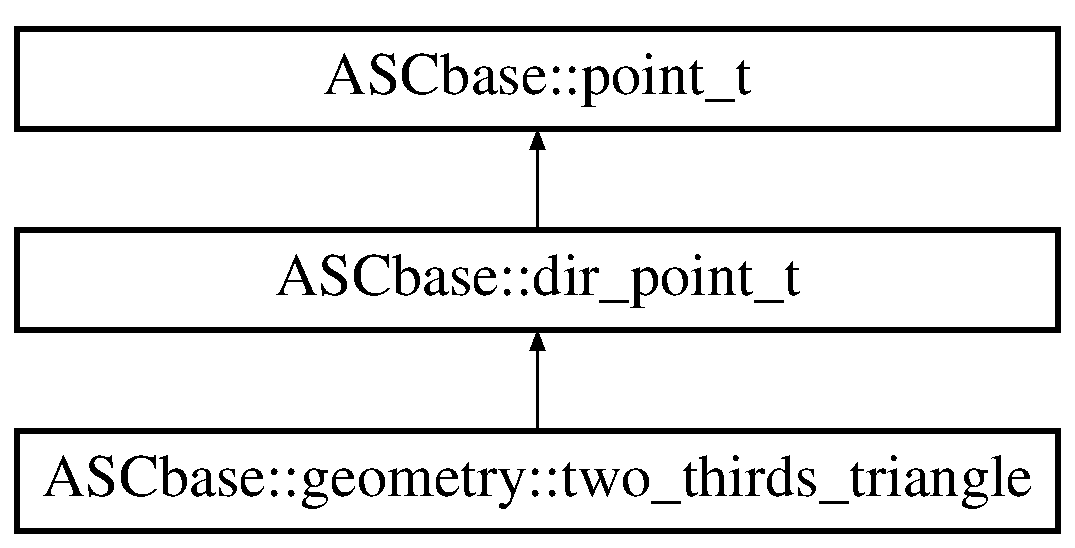
\includegraphics[height=3cm]{classASCbase_1_1geometry_1_1two__thirds__triangle}
\end{center}
\end{figure}
\subsection*{Public Member Functions}
\begin{CompactItemize}
\item 
\textbf{two\_\-thirds\_\-triangle} (alloc\_\-t a=ALLOC\_\-POSITION)\label{classASCbase_1_1geometry_1_1two__thirds__triangle_c5b749d578f384ebb2f2ebf06b136dad}

\item 
\textbf{two\_\-thirds\_\-triangle} (const \bf{two\_\-thirds\_\-triangle} \&p)\label{classASCbase_1_1geometry_1_1two__thirds__triangle_61c17246665ba11761bd28a36450b746}

\item 
const \bf{two\_\-thirds\_\-triangle} \& \textbf{operator=} (const \bf{two\_\-thirds\_\-triangle} \&p)\label{classASCbase_1_1geometry_1_1two__thirds__triangle_e4ddddeffcae8e96e30cbe475fc04265}

\end{CompactItemize}
\subsection*{Public Attributes}
\begin{CompactItemize}
\item 
int \bf{triangle\_\-index}\label{classASCbase_1_1geometry_1_1two__thirds__triangle_0f34a791ed7ba9f1e116a12da68b1bff}

\begin{CompactList}\small\item\em Index of the triangle in the input file. \item\end{CompactList}\end{CompactItemize}
\subsection*{Private Member Functions}
\begin{CompactItemize}
\item 
void \textbf{do\_\-copy} (const \bf{two\_\-thirds\_\-triangle} \&p)\label{classASCbase_1_1geometry_1_1two__thirds__triangle_590f608270791925a9e65210cd3bcc26}

\end{CompactItemize}


\subsection{Detailed Description}
Simple derived class that gives us a unique number for 2/3rds of triangle. 



The documentation for this class was generated from the following file:\begin{CompactItemize}
\item 
Immovable\-Trimesh.H\end{CompactItemize}

\section{ASCbase::Union\-Of\-Balls Class Reference}
\label{classASCbase_1_1UnionOfBalls}\index{ASCbase::UnionOfBalls@{ASCbase::UnionOfBalls}}
Union of spherical solids bounding volume.  


{\tt \#include $<$Bounding\-Volume.H$>$}

Inheritance diagram for ASCbase::Union\-Of\-Balls::\begin{figure}[H]
\begin{center}
\leavevmode
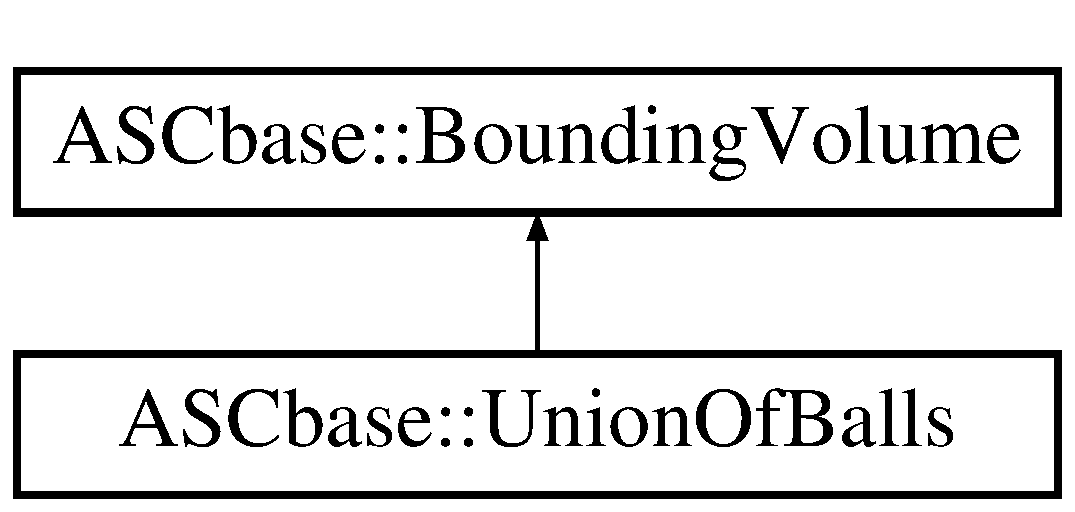
\includegraphics[height=2cm]{classASCbase_1_1UnionOfBalls}
\end{center}
\end{figure}
\subsection*{Public Member Functions}
\begin{CompactItemize}
\item 
\textbf{Union\-Of\-Balls} (const size\_\-t num\_\-balls, const my\_\-float\_\-t $\ast$centers, const my\_\-float\_\-t $\ast$radii)\label{classASCbase_1_1UnionOfBalls_bdf71b8d8aa0c447e35e7b61b577f56c}

\item 
\textbf{Union\-Of\-Balls} (const \bf{Coord\-File} \&mol, const my\_\-float\_\-t tol=3.0)\label{classASCbase_1_1UnionOfBalls_93603c0f91e9a901bcf55ed17183f974}

\item 
\textbf{Union\-Of\-Balls} (const \bf{Union\-Of\-Balls} \&src)\label{classASCbase_1_1UnionOfBalls_525cc26074e6e938ee3f8e0a00580df5}

\item 
virtual bool \bf{contains} (const my\_\-float\_\-t $\ast$point) const \label{classASCbase_1_1UnionOfBalls_35d7a6372c343fd49af508223540dbfe}

\begin{CompactList}\small\item\em Is the given point inside the bounding volume? \item\end{CompactList}\item 
virtual bool \textbf{BIND\_\-vol\_\-contains} (const my\_\-float\_\-t $\ast$point) const \label{classASCbase_1_1UnionOfBalls_062e19950a34f2c92756ddd474d17db4}

\item 
virtual bool \textbf{RAD\_\-vol\_\-contains} (const my\_\-float\_\-t $\ast$point) const \label{classASCbase_1_1UnionOfBalls_85d46140c2f090aecb2e9b2970bc71c1}

\item 
virtual size\_\-t \bf{discretize} (const my\_\-float\_\-t spacing, my\_\-float\_\-t $\ast$$\ast$grid\_\-pts)\label{classASCbase_1_1UnionOfBalls_5f3ca248e1e5e8554dae45ac5c426c28}

\begin{CompactList}\small\item\em discretize the volume using the spacing for grid spacing. \item\end{CompactList}\item 
virtual std::string \textbf{xml\_\-str} ()\label{classASCbase_1_1UnionOfBalls_84e656c9ff4fef4f7a4707495715ff70}

\end{CompactItemize}
\subsection*{Private Member Functions}
\begin{CompactItemize}
\item 
void \textbf{init} ()\label{classASCbase_1_1UnionOfBalls_a98c168b667d7298c29037933b10b922}

\item 
void \textbf{clear} ()\label{classASCbase_1_1UnionOfBalls_e6fcd15076dd64afce01a77027ee1ef9}

\end{CompactItemize}
\subsection*{Private Attributes}
\begin{CompactItemize}
\item 
my\_\-float\_\-t $\ast$ \textbf{A\_\-centers\_\-begin}\label{classASCbase_1_1UnionOfBalls_5bc57d328307b5bd8599468bc102c974}

\item 
my\_\-float\_\-t $\ast$ \textbf{A\_\-centers\_\-end}\label{classASCbase_1_1UnionOfBalls_45abbdda1436d8cf9a6307475e1f981e}

\item 
my\_\-float\_\-t $\ast$ \textbf{A\_\-radii\_\-squared}\label{classASCbase_1_1UnionOfBalls_483337996767271d2a28f3142abed396}

\item 
my\_\-float\_\-t \textbf{A\_\-BIND\_\-rad\_\-squared}\label{classASCbase_1_1UnionOfBalls_70cef8b0e9a4fb07652d525127589a33}

\item 
my\_\-float\_\-t \textbf{A\_\-RAD\_\-rad\_\-squared}\label{classASCbase_1_1UnionOfBalls_0e1c4804bf021db5e7f641e9316a6226}

\end{CompactItemize}


\subsection{Detailed Description}
Union of spherical solids bounding volume. 



The documentation for this class was generated from the following files:\begin{CompactItemize}
\item 
Bounding\-Volume.H\item 
Bounding\-Volume.C\end{CompactItemize}

\section{ASCbase::geometry::Vert\-Attrib Class Reference}
\label{classASCbase_1_1geometry_1_1VertAttrib}\index{ASCbase::geometry::VertAttrib@{ASCbase::geometry::VertAttrib}}
A class to hold attributes associated with a vertex.  


{\tt \#include $<$Vert\-Attrib.H$>$}

Inheritance diagram for ASCbase::geometry::Vert\-Attrib::\begin{figure}[H]
\begin{center}
\leavevmode
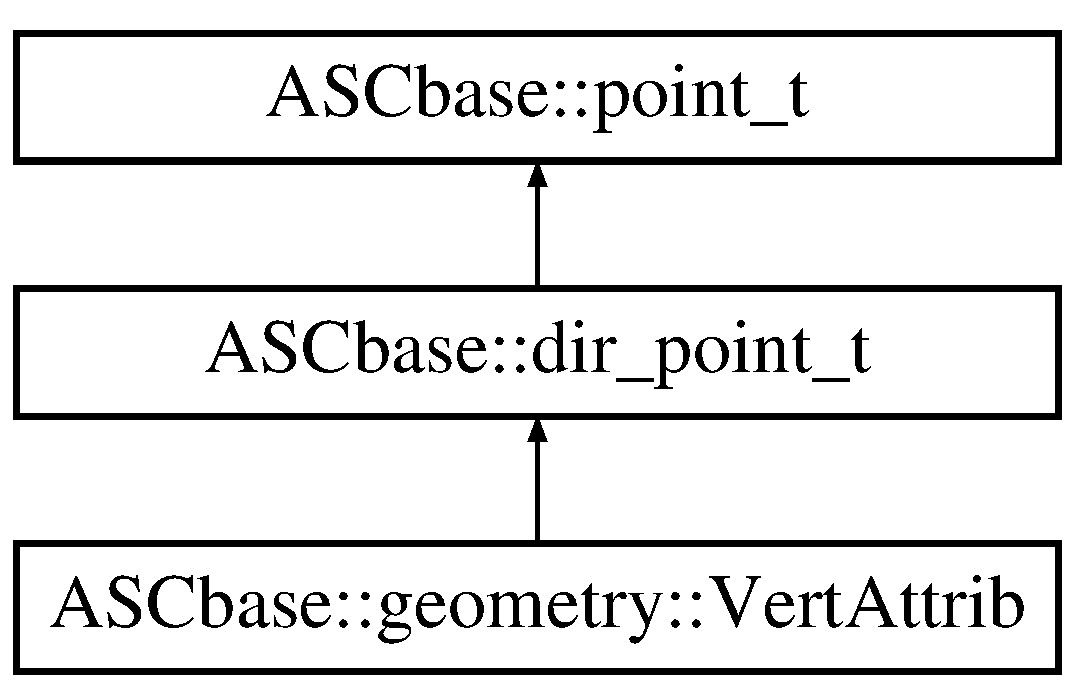
\includegraphics[height=3cm]{classASCbase_1_1geometry_1_1VertAttrib}
\end{center}
\end{figure}
\subsection*{Public Types}
\begin{CompactItemize}
\item 
typedef \bf{dir\_\-point\_\-storage}$<$ \bf{Vert\-Attrib} $>$::iterator \bf{vi}\label{classASCbase_1_1geometry_1_1VertAttrib_d3308c2a5ee7edecf77e42c012d06dc9}

\begin{CompactList}\small\item\em Iterator into a \doxyref{dir\_\-point\_\-storage}{p.}{classASCbase_1_1dir__point__storage} holding vertices. \item\end{CompactList}\item 
typedef \bf{dir\_\-point\_\-storage}$<$ \bf{Vert\-Attrib} $>$::const\_\-iterator \bf{vci}\label{classASCbase_1_1geometry_1_1VertAttrib_1e901e3461cadbcb3783f47d9b9cb3fb}

\begin{CompactList}\small\item\em Const iterator into a \doxyref{dir\_\-point\_\-storage}{p.}{classASCbase_1_1dir__point__storage} holding vertices. \item\end{CompactList}\end{CompactItemize}
\subsection*{Public Member Functions}
\begin{CompactItemize}
\item 
\bf{Vert\-Attrib} (alloc\_\-t a=ALLOC\_\-POSITION)\label{classASCbase_1_1geometry_1_1VertAttrib_a77e8939222aed943aebbe5e245e470a}

\begin{CompactList}\small\item\em Default constructor. \item\end{CompactList}\item 
\bf{Vert\-Attrib} (const \bf{Vert\-Attrib} \&V)\label{classASCbase_1_1geometry_1_1VertAttrib_8e26a0cf88068110941e381fc5733821}

\begin{CompactList}\small\item\em Copy constructor. \item\end{CompactList}\item 
const \bf{Vert\-Attrib} \& \bf{operator=} (const \bf{Vert\-Attrib} \&V)\label{classASCbase_1_1geometry_1_1VertAttrib_65a6cc95baa1a297f7dd96edb4b6aac2}

\begin{CompactList}\small\item\em Assignment operator. \item\end{CompactList}\end{CompactItemize}
\subsection*{Static Public Attributes}
\begin{CompactItemize}
\item 
static \bf{dir\_\-point\_\-storage}$<$ \bf{Vert\-Attrib} $>$ \textbf{NULL\_\-VERTICES\_\-STORAGE}\label{classASCbase_1_1geometry_1_1VertAttrib_088f49b73498b97a1b34b305aaff2da7}

\item 
static const \bf{vi} \textbf{NULL\_\-VI}
\item 
static const \bf{vci} \textbf{NULL\_\-VCI}
\end{CompactItemize}
\subsection*{Private Member Functions}
\begin{CompactItemize}
\item 
void \textbf{do\_\-copy} (const \bf{Vert\-Attrib} \&V)\label{classASCbase_1_1geometry_1_1VertAttrib_51ee7574637a50f55de61267beec3eff}

\end{CompactItemize}


\subsection{Detailed Description}
A class to hold attributes associated with a vertex. 



\subsection{Member Data Documentation}
\index{ASCbase::geometry::VertAttrib@{ASCbase::geometry::Vert\-Attrib}!NULL_VCI@{NULL\_\-VCI}}
\index{NULL_VCI@{NULL\_\-VCI}!ASCbase::geometry::VertAttrib@{ASCbase::geometry::Vert\-Attrib}}
\subsubsection{\setlength{\rightskip}{0pt plus 5cm}const \bf{Vert\-Attrib::vci} Vert\-Attrib::NULL\_\-VCI\hspace{0.3cm}{\tt  [static]}}\label{classASCbase_1_1geometry_1_1VertAttrib_e8eb59ab0360806526181b51ef95a24a}


\textbf{Initial value:}

\begin{Code}\begin{verbatim} 
  VertAttrib::NULL_VERTICES_STORAGE.end()
\end{verbatim}\end{Code}
\index{ASCbase::geometry::VertAttrib@{ASCbase::geometry::Vert\-Attrib}!NULL_VI@{NULL\_\-VI}}
\index{NULL_VI@{NULL\_\-VI}!ASCbase::geometry::VertAttrib@{ASCbase::geometry::Vert\-Attrib}}
\subsubsection{\setlength{\rightskip}{0pt plus 5cm}const \bf{Vert\-Attrib::vi} Vert\-Attrib::NULL\_\-VI\hspace{0.3cm}{\tt  [static]}}\label{classASCbase_1_1geometry_1_1VertAttrib_7b134c2fc83291f59490109ff62b9856}


\textbf{Initial value:}

\begin{Code}\begin{verbatim} 
  VertAttrib::NULL_VERTICES_STORAGE.end()
\end{verbatim}\end{Code}


The documentation for this class was generated from the following files:\begin{CompactItemize}
\item 
Vert\-Attrib.H\item 
Vert\-Attrib.C\end{CompactItemize}

\section{ASCbase::geometry::vertex\_\-t Class Reference}
\label{classASCbase_1_1geometry_1_1vertex__t}\index{ASCbase::geometry::vertex_t@{ASCbase::geometry::vertex\_\-t}}
Might be better named \char`\"{}node\char`\"{}?  


{\tt \#include $<$Tri\-Mesh\-Sphere.H$>$}

Inheritance diagram for ASCbase::geometry::vertex\_\-t::\begin{figure}[H]
\begin{center}
\leavevmode
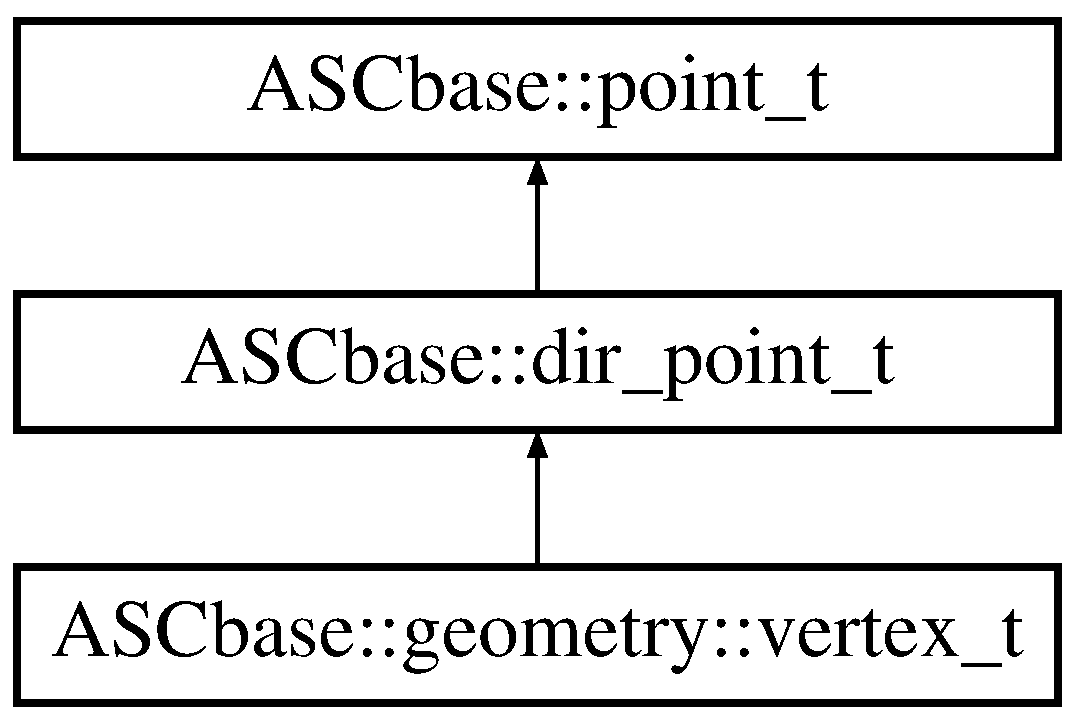
\includegraphics[height=3cm]{classASCbase_1_1geometry_1_1vertex__t}
\end{center}
\end{figure}
\subsection*{Public Member Functions}
\begin{CompactItemize}
\item 
\textbf{vertex\_\-t} (alloc\_\-t a=ALLOC\_\-POSITION)\label{classASCbase_1_1geometry_1_1vertex__t_b26d405918f18263845710e1cbdbd478}

\item 
\textbf{vertex\_\-t} (const \bf{vertex\_\-t} \&v)\label{classASCbase_1_1geometry_1_1vertex__t_369761b4291cb2a821f12dd56e409eb7}

\item 
const \bf{vertex\_\-t} \& \textbf{operator=} (const \bf{vertex\_\-t} \&v)\label{classASCbase_1_1geometry_1_1vertex__t_9073d65a8993b63729b0ddea759c7cd6}

\item 
void \textbf{setup\_\-one\_\-ring} (half\_\-edge\_\-vci beg\_\-in, half\_\-edge\_\-vci end\_\-in)\label{classASCbase_1_1geometry_1_1vertex__t_10f4bc8c2b1f885ebe29a995acdb3d31}

\item 
bool \textbf{inside\_\-one\_\-ring} (const my\_\-float\_\-t $\ast$pt)\label{classASCbase_1_1geometry_1_1vertex__t_107f530235423b366efbcd69c33d8f21}

\end{CompactItemize}
\subsection*{Private Attributes}
\begin{CompactItemize}
\item 
std::list$<$ half\_\-edge\_\-vci $>$ \textbf{A\_\-one\_\-ring\_\-edges}\label{classASCbase_1_1geometry_1_1vertex__t_9d8c7fb281ada6fd0369cda6007d3f55}

\end{CompactItemize}


\subsection{Detailed Description}
Might be better named \char`\"{}node\char`\"{}? 



The documentation for this class was generated from the following file:\begin{CompactItemize}
\item 
Tri\-Mesh\-Sphere.H\end{CompactItemize}

\section{ASCbase::Water\-Points Class Reference}
\label{classASCbase_1_1WaterPoints}\index{ASCbase::WaterPoints@{ASCbase::WaterPoints}}
Setup a data class for placing water hbond points.  


{\tt \#include $<$Water\-Points.H$>$}

\subsection*{Public Member Functions}
\begin{CompactItemize}
\item 
\bf{Water\-Points} ()\label{classASCbase_1_1WaterPoints_1e8c62ea849bff31c173ef1aeb4a0793}

\begin{CompactList}\small\item\em Setup the hard coded relative positions for water hbond points. \item\end{CompactList}\item 
void \bf{transform} (const my\_\-float\_\-t $\ast$R, const my\_\-float\_\-t $\ast$T)
\item 
void \bf{inverse\_\-transform} (const my\_\-float\_\-t $\ast$R, const my\_\-float\_\-t $\ast$T)
\item 
void \bf{revert} ()
\item 
hbond\_\-ideal\_\-pt\_\-vec::const\_\-iterator \textbf{ideal\_\-pts\_\-begin} () const \label{classASCbase_1_1WaterPoints_f65c3e88f37976c4fe26a19873064d16}

\item 
hbond\_\-ideal\_\-pt\_\-vec::const\_\-iterator \textbf{ideal\_\-pts\_\-end} () const \label{classASCbase_1_1WaterPoints_6343e72889915476801eeb9210cc691b}

\end{CompactItemize}
\subsection*{Private Attributes}
\begin{CompactItemize}
\item 
\bf{hbond\_\-fit\_\-pt\_\-vec} \textbf{water\_\-pts}\label{classASCbase_1_1WaterPoints_05e17c99a13206483c15d0d640bebf9e}

\item 
\bf{hbond\_\-ideal\_\-pt\_\-vec} \textbf{water\_\-ideal\_\-pts}\label{classASCbase_1_1WaterPoints_b5125b530f71709362fb5b26847becb2}

\end{CompactItemize}
\subsection*{Static Private Attributes}
\begin{CompactItemize}
\item 
static const uint \bf{num\_\-pts} = 20\label{classASCbase_1_1WaterPoints_a96d16672c2be18eb651e9594045a30d}

\begin{CompactList}\small\item\em Number of 3D points in realtive\_\-pos. \item\end{CompactList}\item 
static const my\_\-float\_\-t \bf{relative\_\-pos} [$\,$]
\begin{CompactList}\small\item\em Relative pos of H2O hbond pts. \item\end{CompactList}\item 
static const my\_\-float\_\-t \bf{relative\_\-dir} [$\,$]
\begin{CompactList}\small\item\em Relative dir of H2O hbond pts. \item\end{CompactList}\end{CompactItemize}


\subsection{Detailed Description}
Setup a data class for placing water hbond points. 

This seems like a more straightforward way of doing things, but because the hydrogen bonding method is already done for residues and it is not a significant portion (in terms of computational speed) of the template generation process there is no pressing need to change it 



\subsection{Member Function Documentation}
\index{ASCbase::WaterPoints@{ASCbase::Water\-Points}!inverse_transform@{inverse\_\-transform}}
\index{inverse_transform@{inverse\_\-transform}!ASCbase::WaterPoints@{ASCbase::Water\-Points}}
\subsubsection{\setlength{\rightskip}{0pt plus 5cm}void ASCbase::Water\-Points::inverse\_\-transform (const my\_\-float\_\-t $\ast$ {\em R}, const my\_\-float\_\-t $\ast$ {\em T})\hspace{0.3cm}{\tt  [inline]}}\label{classASCbase_1_1WaterPoints_af926b1ccfc8db7ae215209d006e338b}


Transform the positions and directions for the water hbond points by the inverse of the rigid transformation defined by R and T. \index{ASCbase::WaterPoints@{ASCbase::Water\-Points}!revert@{revert}}
\index{revert@{revert}!ASCbase::WaterPoints@{ASCbase::Water\-Points}}
\subsubsection{\setlength{\rightskip}{0pt plus 5cm}void ASCbase::Water\-Points::revert ()\hspace{0.3cm}{\tt  [inline]}}\label{classASCbase_1_1WaterPoints_ecc516195eeee66daeb5232b79566bb3}


Revert the water points back to the positions relative to the oxygen in H2O \index{ASCbase::WaterPoints@{ASCbase::Water\-Points}!transform@{transform}}
\index{transform@{transform}!ASCbase::WaterPoints@{ASCbase::Water\-Points}}
\subsubsection{\setlength{\rightskip}{0pt plus 5cm}void ASCbase::Water\-Points::transform (const my\_\-float\_\-t $\ast$ {\em R}, const my\_\-float\_\-t $\ast$ {\em T})\hspace{0.3cm}{\tt  [inline]}}\label{classASCbase_1_1WaterPoints_28e85993b24ad7d2d9f690972b399d19}


Transform the positions and directions for the water hbond points given the rigid transformation defined by R and T. 

\subsection{Member Data Documentation}
\index{ASCbase::WaterPoints@{ASCbase::Water\-Points}!relative_dir@{relative\_\-dir}}
\index{relative_dir@{relative\_\-dir}!ASCbase::WaterPoints@{ASCbase::Water\-Points}}
\subsubsection{\setlength{\rightskip}{0pt plus 5cm}const my\_\-float\_\-t \bf{Water\-Points::relative\_\-dir}\hspace{0.3cm}{\tt  [static, private]}}\label{classASCbase_1_1WaterPoints_9983412b6966d9c04890f819f3512332}


\textbf{Initial value:}

\begin{Code}\begin{verbatim} 
  { 0.6206,  0.7841,  0.0000,
    0.3150,  0.9491,  0.0000,
    0.8514,  0.5246,  0.0000,
    0.5832,  0.7368,  0.3420,
    0.5832,  0.7368, -0.3420,
    0.6206, -0.7841,  0.0000,
    0.8514, -0.5246,  0.0000,
    0.3150, -0.9491,  0.0000,
    0.5832, -0.7368,  0.3420,
    0.5832, -0.7368, -0.3420,
   -0.5771,  0.0000,  0.8166,
   -0.5423, -0.3420,  0.7674,
   -0.5423,  0.3420,  0.7674,
   -0.2630,  0.0000,  0.9648,
   -0.8216,  0.0000,  0.5700,
   -0.5771,  0.0000, -0.8166,
   -0.5423, -0.3420, -0.7674,
   -0.5423,  0.3420, -0.7674,
   -0.8216,  0.0000, -0.5700,
   -0.2630,  0.0000, -0.9648
  }
\end{verbatim}\end{Code}
Relative dir of H2O hbond pts. 

\index{ASCbase::WaterPoints@{ASCbase::Water\-Points}!relative_pos@{relative\_\-pos}}
\index{relative_pos@{relative\_\-pos}!ASCbase::WaterPoints@{ASCbase::Water\-Points}}
\subsubsection{\setlength{\rightskip}{0pt plus 5cm}const my\_\-float\_\-t \bf{Water\-Points::relative\_\-pos}\hspace{0.3cm}{\tt  [static, private]}}\label{classASCbase_1_1WaterPoints_00f83dfce139f11e124c5258a68ffc7b}


\textbf{Initial value:}

\begin{Code}\begin{verbatim} 
  { 1.8618,  2.3524,  0.0000,
    0.9450,  2.8473,  0.0000,
    2.5541,  1.5737,  0.0000,
    1.7495,  2.2105,  1.0261,
    1.7495,  2.2105, -1.0261,
    1.8618, -2.3524,  0.0000,
    2.5541, -1.5737,  0.0000,
    0.9450, -2.8473,  0.0000,
    1.7495, -2.2105,  1.0261,
    1.7495, -2.2105, -1.0261,
   -1.7314,  0.0000,  2.4499,
   -1.6270, -1.0261,  2.3022,
   -1.6270,  1.0261,  2.3022,
   -0.7891,  0.0000,  2.8944,
   -2.4649,  0.0000,  1.7100,
   -1.7314,  0.0000, -2.4499,
   -1.6270, -1.0261, -2.3022,
   -1.6270,  1.0261, -2.3022,
   -2.4649,  0.0000, -1.7100,
   -0.7891,  0.0000, -2.8944
  }
\end{verbatim}\end{Code}
Relative pos of H2O hbond pts. 



The documentation for this class was generated from the following files:\begin{CompactItemize}
\item 
Water\-Points.H\item 
Water\-Points.C\end{CompactItemize}

\section{ASCbase::Weighted\-Sums\-Score Class Reference}
\label{classASCbase_1_1WeightedSumsScore}\index{ASCbase::WeightedSumsScore@{ASCbase::WeightedSumsScore}}
Weight interaction NN interaction pair sums.  


{\tt \#include $<$Weighted\-Sums\-Score.H$>$}

Inheritance diagram for ASCbase::Weighted\-Sums\-Score::\begin{figure}[H]
\begin{center}
\leavevmode
\includegraphics[height=3cm]{classASCbase_1_1WeightedSumsScore}
\end{center}
\end{figure}
\subsection*{Public Types}
\begin{CompactItemize}
\item 
typedef std::less$<$ my\_\-float\_\-t $>$ \textbf{score\_\-cmp}\label{classASCbase_1_1WeightedSumsScore_c7d40e189ef4573833fd970f05ca0f26}

\end{CompactItemize}
\subsection*{Public Member Functions}
\begin{CompactItemize}
\item 
\bf{Weighted\-Sums\-Score} ()\label{classASCbase_1_1WeightedSumsScore_69c71746b50e336c3bfeea4db657832c}

\begin{CompactList}\small\item\em Default constructor for site map point scoring of (aligned) sitemaps. \item\end{CompactList}\item 
virtual \bf{$\sim$Weighted\-Sums\-Score} ()\label{classASCbase_1_1WeightedSumsScore_69dc18855ceef71681dd7a00e8f0966b}

\begin{CompactList}\small\item\em basic destruction \item\end{CompactList}\item 
my\_\-float\_\-t \bf{score} (const \bf{Model\-Sitemap} \&model, const \bf{Dbase\-Sitemap} \&dbase, \bf{rigid\_\-align\_\-t} $\ast$scores)
\item 
virtual my\_\-float\_\-t \bf{correspondences} (const \bf{Model\-Sitemap} \&model, my\_\-float\_\-t $\ast$$\ast$Q\_\-pts\_\-ptr, my\_\-float\_\-t $\ast$$\ast$D\_\-pts\_\-ptr, size\_\-t $\ast$npts)\label{classASCbase_1_1WeightedSumsScore_14bd722eaf99ae7c9c81fe85e5f761d6}

\begin{CompactList}\small\item\em Get the latest correspondences of the db to query sites. \item\end{CompactList}\item 
virtual void \textbf{polar\_\-correspondences} (const \bf{Model\-Sitemap} \&model, std::vector$<$ const my\_\-float\_\-t $\ast$ $>$ $\ast$q\_\-pts, std::vector$<$ const my\_\-float\_\-t $\ast$ $>$ $\ast$corr\_\-pts) const \label{classASCbase_1_1WeightedSumsScore_76c3b03103218cc983b2233952bdaf45}

\item 
virtual bool \bf{uses\_\-surface\_\-mesh} ()
\item 
virtual bool \bf{uses\_\-hbond\_\-surfaces} ()
\end{CompactItemize}
\subsection*{Protected Member Functions}
\begin{CompactItemize}
\item 
virtual const my\_\-float\_\-t $\ast$ \textbf{closest\_\-points} () const \label{classASCbase_1_1WeightedSumsScore_d82af6105e9ee622ed5c122825a2d3e7}

\item 
virtual int \textbf{num\_\-close\_\-points} () const \label{classASCbase_1_1WeightedSumsScore_0b305cbc0f32afbd99e02ddaeff23962}

\end{CompactItemize}
\subsection*{Private Member Functions}
\begin{CompactItemize}
\item 
void \textbf{init} ()\label{classASCbase_1_1WeightedSumsScore_00168176078d947da51ed3330b164c0b}

\item 
void \textbf{clear\_\-mem} ()\label{classASCbase_1_1WeightedSumsScore_6863b16bbf29f54e2d6de68aa2919e12}

\item 
void \textbf{init\_\-storage} (const \bf{Model\-Sitemap} \&model)\label{classASCbase_1_1WeightedSumsScore_672e6390f1323736b8890726bc1dd0e6}

\end{CompactItemize}
\subsection*{Private Attributes}
\begin{CompactItemize}
\item 
my\_\-float\_\-t $\ast$ \textbf{A\_\-closest\_\-pts}\label{classASCbase_1_1WeightedSumsScore_b4555ac1476234e3c94e7e221c33bd9f}

\item 
my\_\-float\_\-t $\ast$ \textbf{A\_\-pt\_\-dists}\label{classASCbase_1_1WeightedSumsScore_0c66f4e146c2ef22497d555d99634edb}

\item 
size\_\-t \textbf{A\_\-max\_\-num\_\-pts}\label{classASCbase_1_1WeightedSumsScore_9c0082cdfc124ac7037256429ccdc230}

\end{CompactItemize}
\subsection*{Static Private Attributes}
\begin{CompactItemize}
\item 
static const std::string \bf{A\_\-fname} = \char`\"{}Weighted\-Sums\-Score.C\char`\"{}\label{classASCbase_1_1WeightedSumsScore_a55eaafd22a87ff837e6fdc31d7d9ffd}

\begin{CompactList}\small\item\em Source file name. \item\end{CompactList}\item 
static const my\_\-float\_\-t \bf{POLAR\_\-SUM\_\-W} = 0.0\label{classASCbase_1_1WeightedSumsScore_0ddbb39dee8f32733be5f250cfe28b21}

\begin{CompactList}\small\item\em W for sum all \char`\"{}good\char`\"{} polar interactions. \item\end{CompactList}\item 
static const my\_\-float\_\-t \bf{DD\_\-OR\_\-AA\_\-POLAR\_\-SUM\_\-W} = -0.0456776\label{classASCbase_1_1WeightedSumsScore_0ab2b57fc4cb8e676ca80141d5a6cf01}

\begin{CompactList}\small\item\em W for sum only DD or AA \char`\"{}good\char`\"{} polar interactions. \item\end{CompactList}\item 
static const my\_\-float\_\-t \bf{DONEPTOR\_\-POLAR\_\-SUM\_\-W} = -0.012702\label{classASCbase_1_1WeightedSumsScore_6d6a766de6d9e26acb5ac25901434b12}

\begin{CompactList}\small\item\em W for sum NA or AN or ND or DN or NN \char`\"{}good\char`\"{} polar interactions. \item\end{CompactList}\item 
static const my\_\-float\_\-t \bf{HPHOBIC\_\-COUNT\_\-W} = -0.0323914\label{classASCbase_1_1WeightedSumsScore_a955731ebec450fedd1992c26dd9db3c}

\begin{CompactList}\small\item\em W for hydrophobic point count. \item\end{CompactList}\item 
static const my\_\-float\_\-t \bf{POLAR\_\-MISMATCH\_\-W} = 0.0\label{classASCbase_1_1WeightedSumsScore_357f45b79bcb254cff96666a4539e223}

\begin{CompactList}\small\item\em W for sum of AD or DA matches with positive dot product. \item\end{CompactList}\item 
static const my\_\-float\_\-t \bf{UNSAT\_\-POLAR\_\-W} = 0.0\label{classASCbase_1_1WeightedSumsScore_2f6797c0e1495883fb50768a5a4307d4}

\begin{CompactList}\small\item\em W for polar points matched to hydrophobic. \item\end{CompactList}\item 
static const my\_\-float\_\-t \bf{CONSTANT\_\-TERM} = 0.0054731\label{classASCbase_1_1WeightedSumsScore_aeac1f99a57289ddf2001453c1e77bf4}

\begin{CompactList}\small\item\em Constant obtained from the regresion method. \item\end{CompactList}\item 
static const my\_\-float\_\-t \bf{SCALED\_\-POLAR\_\-SUM\_\-W} = 0.0\label{classASCbase_1_1WeightedSumsScore_917b2edf7bc9d6b9388a6cf35ac34984}

\begin{CompactList}\small\item\em W for sum all \char`\"{}good\char`\"{} polar interactions for scaled terms. \item\end{CompactList}\item 
static const my\_\-float\_\-t \bf{SCALED\_\-DD\_\-OR\_\-AA\_\-POLAR\_\-SUM\_\-W} = -1.39892\label{classASCbase_1_1WeightedSumsScore_a55423586953effb70d9ffa4c409ebbc}

\begin{CompactList}\small\item\em W for sum only DD or AA \char`\"{}good\char`\"{} polar interactions for scaled terms. \item\end{CompactList}\item 
static const my\_\-float\_\-t \bf{SCALED\_\-DONEPTOR\_\-POLAR\_\-SUM\_\-W} = 0.0329575\label{classASCbase_1_1WeightedSumsScore_480239bd6df13b6088fa7f2514c544a1}

\begin{CompactList}\small\item\em W for sum NA or AN or ND or DN or NN \char`\"{}good\char`\"{} polar interactions for scaled terms. \item\end{CompactList}\item 
static const my\_\-float\_\-t \bf{SCALED\_\-HPHOBIC\_\-COUNT\_\-W} = -0.367527\label{classASCbase_1_1WeightedSumsScore_df981a43a0b9ea8637d3713222baecd7}

\begin{CompactList}\small\item\em W for hydrophobic point count for scaled terms. \item\end{CompactList}\item 
static const my\_\-float\_\-t \bf{SCALED\_\-POLAR\_\-MISMATCH\_\-W} = 0.0\label{classASCbase_1_1WeightedSumsScore_ba7f330b50d3250a1355c7f56b94af9f}

\begin{CompactList}\small\item\em W for sum of AD or DA matches with positive dot product for scaled terms. \item\end{CompactList}\item 
static const my\_\-float\_\-t \bf{SCALED\_\-UNSAT\_\-POLAR\_\-W} = 0.0\label{classASCbase_1_1WeightedSumsScore_0dffcb3e686f38d0f66b7cc2f10a89dc}

\begin{CompactList}\small\item\em W for polar points matched to hydrophobic for scaled terms. \item\end{CompactList}\item 
static const my\_\-float\_\-t \bf{SCALED\_\-CONSTANT\_\-TERM} = 0.0373266\label{classASCbase_1_1WeightedSumsScore_e0a90bb30eeb2d8117323d04a4cff22b}

\begin{CompactList}\small\item\em Constant obtained from the regresion method for scaled terms. \item\end{CompactList}\item 
static const my\_\-float\_\-t \bf{A\_\-max\_\-dist} = 1.5\label{classASCbase_1_1WeightedSumsScore_d5f1b812740954ec65df1828fd1e522a}

\begin{CompactList}\small\item\em Max distance for corresponding points. \item\end{CompactList}\end{CompactItemize}


\subsection{Detailed Description}
Weight interaction NN interaction pair sums. 



\subsection{Member Function Documentation}
\index{ASCbase::WeightedSumsScore@{ASCbase::Weighted\-Sums\-Score}!score@{score}}
\index{score@{score}!ASCbase::WeightedSumsScore@{ASCbase::Weighted\-Sums\-Score}}
\subsubsection{\setlength{\rightskip}{0pt plus 5cm}my\_\-float\_\-t ASCbase::Weighted\-Sums\-Score::score (const \bf{Model\-Sitemap} \& {\em model}, const \bf{Dbase\-Sitemap} \& {\em dbase}, \bf{rigid\_\-align\_\-t} $\ast$ {\em scores})\hspace{0.3cm}{\tt  [inline, virtual]}}\label{classASCbase_1_1WeightedSumsScore_eeee8c834449ce75686bb076f40c3ee4}


\begin{Desc}
\item[Parameters:]
\begin{description}
\item[{\em model}]Const ref to the model site \item[{\em dbase}]Const ref to the sitemap aligned to the model sitemap \item[{\em scores}]iterator to the score data class \item[{\em save\_\-correspondences}]should the score method save the points correspondences? Saving is required for methods like ICP \end{description}
\end{Desc}
\begin{Desc}
\item[Returns:]The score of the alignment \end{Desc}


Implements \bf{ASCbase::Sites\-Score\-Base} \doxyref{p.}{classASCbase_1_1SitesScoreBase_651f05f08e15b7ea8f7fa7c41973499e}.

Reimplemented in \bf{ASCbase::point\_\-and\_\-surf\_\-score} \doxyref{p.}{classASCbase_1_1point__and__surf__score_f7086e180c849bba8a8a1df984a3b114}.\index{ASCbase::WeightedSumsScore@{ASCbase::Weighted\-Sums\-Score}!uses_hbond_surfaces@{uses\_\-hbond\_\-surfaces}}
\index{uses_hbond_surfaces@{uses\_\-hbond\_\-surfaces}!ASCbase::WeightedSumsScore@{ASCbase::Weighted\-Sums\-Score}}
\subsubsection{\setlength{\rightskip}{0pt plus 5cm}virtual bool ASCbase::Weighted\-Sums\-Score::uses\_\-hbond\_\-surfaces ()\hspace{0.3cm}{\tt  [inline, virtual]}}\label{classASCbase_1_1WeightedSumsScore_a54a5a22b71dd4bc14aaf06f7756eca7}


Derived class should return false, unless the derived class is using the hydrogen bond surface caps 

Reimplemented from \bf{ASCbase::Sites\-Score\-Base} \doxyref{p.}{classASCbase_1_1SitesScoreBase_a7a5fcc3e24663874f8066c00089f3cf}.

Reimplemented in \bf{ASCbase::point\_\-and\_\-surf\_\-score} \doxyref{p.}{classASCbase_1_1point__and__surf__score_8f006a0249c062673acec07465b4d686}.\index{ASCbase::WeightedSumsScore@{ASCbase::Weighted\-Sums\-Score}!uses_surface_mesh@{uses\_\-surface\_\-mesh}}
\index{uses_surface_mesh@{uses\_\-surface\_\-mesh}!ASCbase::WeightedSumsScore@{ASCbase::Weighted\-Sums\-Score}}
\subsubsection{\setlength{\rightskip}{0pt plus 5cm}virtual bool ASCbase::Weighted\-Sums\-Score::uses\_\-surface\_\-mesh ()\hspace{0.3cm}{\tt  [inline, virtual]}}\label{classASCbase_1_1WeightedSumsScore_9d12b648a5adc7dff9d6058d6239a314}


Derived class should return false, unless, the site's surface needs to be to be rotated and translated 

Reimplemented from \bf{ASCbase::Sites\-Score\-Base} \doxyref{p.}{classASCbase_1_1SitesScoreBase_ae4a2a1ae9113bcad0535593c210030f}.

Reimplemented in \bf{ASCbase::point\_\-and\_\-surf\_\-score} \doxyref{p.}{classASCbase_1_1point__and__surf__score_92345073d3e38666cb95cca9adc14ae3}.

The documentation for this class was generated from the following files:\begin{CompactItemize}
\item 
Weighted\-Sums\-Score.H\item 
Weighted\-Sums\-Score.C\end{CompactItemize}

\section{ASCbase::WSS\_\-and\_\-dataset\_\-MP Class Reference}
\label{classASCbase_1_1WSS__and__dataset__MP}\index{ASCbase::WSS_and_dataset_MP@{ASCbase::WSS\_\-and\_\-dataset\_\-MP}}
Weight interaction NN interaction pair sums.  


{\tt \#include $<$WSS\_\-and\_\-dataset\_\-MP.H$>$}

Inheritance diagram for ASCbase::WSS\_\-and\_\-dataset\_\-MP::\begin{figure}[H]
\begin{center}
\leavevmode
\includegraphics[height=3cm]{classASCbase_1_1WSS__and__dataset__MP}
\end{center}
\end{figure}
\subsection*{Public Types}
\begin{CompactItemize}
\item 
typedef std::less$<$ my\_\-float\_\-t $>$ \textbf{score\_\-cmp}\label{classASCbase_1_1WSS__and__dataset__MP_f17104e906fa8b27692f8956cb88c5f6}

\end{CompactItemize}
\subsection*{Public Member Functions}
\begin{CompactItemize}
\item 
\bf{WSS\_\-and\_\-dataset\_\-MP} ()\label{classASCbase_1_1WSS__and__dataset__MP_9dcca2b8b93687cd031fae82a6327ffe}

\begin{CompactList}\small\item\em Default constructor for site map point scoring of (aligned) sitemaps. \item\end{CompactList}\item 
virtual \bf{$\sim$WSS\_\-and\_\-dataset\_\-MP} ()\label{classASCbase_1_1WSS__and__dataset__MP_51cabafd4f5038cb70d9fea0c5e97d49}

\begin{CompactList}\small\item\em basic destruction \item\end{CompactList}\item 
my\_\-float\_\-t \bf{score} (const \bf{Model\-Sitemap} \&model, const \bf{Dbase\-Sitemap} \&dbase, Rigid\-Align\-With\-Dset\-MP $\ast$scores)
\end{CompactItemize}


\subsection{Detailed Description}
Weight interaction NN interaction pair sums. 



\subsection{Member Function Documentation}
\index{ASCbase::WSS_and_dataset_MP@{ASCbase::WSS\_\-and\_\-dataset\_\-MP}!score@{score}}
\index{score@{score}!ASCbase::WSS_and_dataset_MP@{ASCbase::WSS\_\-and\_\-dataset\_\-MP}}
\subsubsection{\setlength{\rightskip}{0pt plus 5cm}my\_\-float\_\-t ASCbase::WSS\_\-and\_\-dataset\_\-MP::score (const \bf{Model\-Sitemap} \& {\em model}, const \bf{Dbase\-Sitemap} \& {\em dbase}, Rigid\-Align\-With\-Dset\-MP $\ast$ {\em scores})\hspace{0.3cm}{\tt  [inline]}}\label{classASCbase_1_1WSS__and__dataset__MP_e25f013ecd47d0e5e3e367f6fa06ea5e}


\begin{Desc}
\item[Parameters:]
\begin{description}
\item[{\em model}]Const ref to the model site \item[{\em dbase}]Const ref to the sitemap aligned to the model sitemap \item[{\em scores}]iterator to the score data class \item[{\em save\_\-correspondences}]should the score method save the points correspondences? Saving is required for methods like ICP \end{description}
\end{Desc}
\begin{Desc}
\item[Returns:]The score of the alignment \end{Desc}


The documentation for this class was generated from the following file:\begin{CompactItemize}
\item 
WSS\_\-and\_\-dataset\_\-MP.H\end{CompactItemize}

\printindex
\end{document}
